\documentclass[twoside]{book}

% Packages required by doxygen
\usepackage{fixltx2e}
\usepackage{calc}
\usepackage{doxygen}
\usepackage[export]{adjustbox} % also loads graphicx
\usepackage{graphicx}
\usepackage[utf8]{inputenc}
\usepackage{makeidx}
\usepackage{multicol}
\usepackage{multirow}
\PassOptionsToPackage{warn}{textcomp}
\usepackage{textcomp}
\usepackage[nointegrals]{wasysym}
\usepackage[table]{xcolor}

% Font selection
\usepackage[T1]{fontenc}
\usepackage[scaled=.90]{helvet}
\usepackage{courier}
\usepackage{amssymb}
\usepackage{sectsty}
\renewcommand{\familydefault}{\sfdefault}
\allsectionsfont{%
  \fontseries{bc}\selectfont%
  \color{darkgray}%
}
\renewcommand{\DoxyLabelFont}{%
  \fontseries{bc}\selectfont%
  \color{darkgray}%
}
\newcommand{\+}{\discretionary{\mbox{\scriptsize$\hookleftarrow$}}{}{}}

% Page & text layout
\usepackage{geometry}
\geometry{%
  a4paper,%
  top=2.5cm,%
  bottom=2.5cm,%
  left=2.5cm,%
  right=2.5cm%
}
\tolerance=750
\hfuzz=15pt
\hbadness=750
\setlength{\emergencystretch}{15pt}
\setlength{\parindent}{0cm}
\setlength{\parskip}{3ex plus 2ex minus 2ex}
\makeatletter
\renewcommand{\paragraph}{%
  \@startsection{paragraph}{4}{0ex}{-1.0ex}{1.0ex}{%
    \normalfont\normalsize\bfseries\SS@parafont%
  }%
}
\renewcommand{\subparagraph}{%
  \@startsection{subparagraph}{5}{0ex}{-1.0ex}{1.0ex}{%
    \normalfont\normalsize\bfseries\SS@subparafont%
  }%
}
\makeatother

% Headers & footers
\usepackage{fancyhdr}
\pagestyle{fancyplain}
\fancyhead[LE]{\fancyplain{}{\bfseries\thepage}}
\fancyhead[CE]{\fancyplain{}{}}
\fancyhead[RE]{\fancyplain{}{\bfseries\leftmark}}
\fancyhead[LO]{\fancyplain{}{\bfseries\rightmark}}
\fancyhead[CO]{\fancyplain{}{}}
\fancyhead[RO]{\fancyplain{}{\bfseries\thepage}}
\fancyfoot[LE]{\fancyplain{}{}}
\fancyfoot[CE]{\fancyplain{}{}}
\fancyfoot[RE]{\fancyplain{}{\bfseries\scriptsize Generated by Doxygen }}
\fancyfoot[LO]{\fancyplain{}{\bfseries\scriptsize Generated by Doxygen }}
\fancyfoot[CO]{\fancyplain{}{}}
\fancyfoot[RO]{\fancyplain{}{}}
\renewcommand{\footrulewidth}{0.4pt}
\renewcommand{\chaptermark}[1]{%
  \markboth{#1}{}%
}
\renewcommand{\sectionmark}[1]{%
  \markright{\thesection\ #1}%
}

% Indices & bibliography
\usepackage{natbib}
\usepackage[titles]{tocloft}
\setcounter{tocdepth}{3}
\setcounter{secnumdepth}{5}
\makeindex

% Hyperlinks (required, but should be loaded last)
\usepackage{ifpdf}
\ifpdf
  \usepackage[pdftex,pagebackref=true]{hyperref}
\else
  \usepackage[ps2pdf,pagebackref=true]{hyperref}
\fi
\hypersetup{%
  colorlinks=true,%
  linkcolor=blue,%
  citecolor=blue,%
  unicode%
}

% Custom commands
\newcommand{\clearemptydoublepage}{%
  \newpage{\pagestyle{empty}\cleardoublepage}%
}

\usepackage{caption}
\captionsetup{labelsep=space,justification=centering,font={bf},singlelinecheck=off,skip=4pt,position=top}

%===== C O N T E N T S =====

\begin{document}

% Titlepage & ToC
\hypersetup{pageanchor=false,
             bookmarksnumbered=true,
             pdfencoding=unicode
            }
\pagenumbering{roman}
\begin{titlepage}
\vspace*{7cm}
\begin{center}%
{\Large jaco \\[1ex]\large 1.\+1.\+0 }\\
\vspace*{1cm}
{\large Generated by Doxygen 1.8.11}\\
\end{center}
\end{titlepage}
\clearemptydoublepage
\tableofcontents
\clearemptydoublepage
\pagenumbering{arabic}
\hypersetup{pageanchor=true}

%--- Begin generated contents ---
\chapter{J\+A\+C\+O-\/\+R\+OS}
\label{md_C:_Users_soli_Downloads_New_folder_kinova-ros-master_README}
\hypertarget{md_C:_Users_soli_Downloads_New_folder_kinova-ros-master_README}{}
\input{md_C:_Users_soli_Downloads_New_folder_kinova-ros-master_README}
\chapter{Namespace Index}
\section{Namespace List}
Here is a list of all namespaces with brief descriptions\+:\begin{DoxyCompactList}
\item\contentsline{section}{\hyperlink{namespace__setup__util}{\+\_\+setup\+\_\+util} }{\pageref{df/dc0/namespace__setup__util}}{}
\item\contentsline{section}{\hyperlink{namespaceadmittance__ctrl}{admittance\+\_\+ctrl} }{\pageref{d7/d0c/namespaceadmittance__ctrl}}{}
\item\contentsline{section}{\hyperlink{namespaceangle__action__client}{angle\+\_\+action\+\_\+client} }{\pageref{d3/d02/namespaceangle__action__client}}{}
\item\contentsline{section}{\hyperlink{namespaceanonymous__namespace_02jaco__arm_8cpp_03}{anonymous\+\_\+namespace\{jaco\+\_\+arm.\+cpp\}} }{\pageref{dd/d9e/namespaceanonymous__namespace_02jaco__arm_8cpp_03}}{}
\item\contentsline{section}{\hyperlink{namespacecartesian__workout}{cartesian\+\_\+workout} }{\pageref{d8/d21/namespacecartesian__workout}}{}
\item\contentsline{section}{\hyperlink{namespacefinger__action__client}{finger\+\_\+action\+\_\+client} }{\pageref{d0/df6/namespacefinger__action__client}}{}
\item\contentsline{section}{\hyperlink{namespacegenerate__cached__setup}{generate\+\_\+cached\+\_\+setup} }{\pageref{d1/d99/namespacegenerate__cached__setup}}{}
\item\contentsline{section}{\hyperlink{namespacegoal__generators}{goal\+\_\+generators} }{\pageref{df/da8/namespacegoal__generators}}{}
\item\contentsline{section}{\hyperlink{namespacegrip__workout}{grip\+\_\+workout} }{\pageref{d0/d38/namespacegrip__workout}}{}
\item\contentsline{section}{\hyperlink{namespacejaco}{jaco} }{\pageref{d4/d3c/namespacejaco}}{}
\item\contentsline{section}{\hyperlink{namespacejaco__demo}{jaco\+\_\+demo} }{\pageref{d3/d0a/namespacejaco__demo}}{}
\item\contentsline{section}{\hyperlink{namespacejaco__driver}{jaco\+\_\+driver} }{\pageref{db/d76/namespacejaco__driver}}{}
\item\contentsline{section}{\hyperlink{namespacejaco__driver_1_1cfg}{jaco\+\_\+driver.\+cfg} }{\pageref{d1/d18/namespacejaco__driver_1_1cfg}}{}
\item\contentsline{section}{\hyperlink{namespacejaco__msgs}{jaco\+\_\+msgs} }{\pageref{d7/dba/namespacejaco__msgs}}{}
\item\contentsline{section}{\hyperlink{namespacejaco__msgs-genmsg-context}{jaco\+\_\+msgs-\/genmsg-\/context} }{\pageref{dd/dc1/namespacejaco__msgs-genmsg-context}}{}
\item\contentsline{section}{\hyperlink{namespacejaco__msgs-msg-paths-context}{jaco\+\_\+msgs-\/msg-\/paths-\/context} }{\pageref{d1/d19/namespacejaco__msgs-msg-paths-context}}{}
\item\contentsline{section}{\hyperlink{namespacejaco__msgs_1_1msg}{jaco\+\_\+msgs.\+msg} }{\pageref{d2/dbe/namespacejaco__msgs_1_1msg}}{}
\item\contentsline{section}{\hyperlink{namespacejaco__msgs_1_1msg_1_1__ArmJointAnglesAction}{jaco\+\_\+msgs.\+msg.\+\_\+\+Arm\+Joint\+Angles\+Action} }{\pageref{d8/d27/namespacejaco__msgs_1_1msg_1_1__ArmJointAnglesAction}}{}
\item\contentsline{section}{\hyperlink{namespacejaco__msgs_1_1msg_1_1__ArmJointAnglesActionFeedback}{jaco\+\_\+msgs.\+msg.\+\_\+\+Arm\+Joint\+Angles\+Action\+Feedback} }{\pageref{d2/d91/namespacejaco__msgs_1_1msg_1_1__ArmJointAnglesActionFeedback}}{}
\item\contentsline{section}{\hyperlink{namespacejaco__msgs_1_1msg_1_1__ArmJointAnglesActionGoal}{jaco\+\_\+msgs.\+msg.\+\_\+\+Arm\+Joint\+Angles\+Action\+Goal} }{\pageref{d8/dec/namespacejaco__msgs_1_1msg_1_1__ArmJointAnglesActionGoal}}{}
\item\contentsline{section}{\hyperlink{namespacejaco__msgs_1_1msg_1_1__ArmJointAnglesActionResult}{jaco\+\_\+msgs.\+msg.\+\_\+\+Arm\+Joint\+Angles\+Action\+Result} }{\pageref{d6/d9a/namespacejaco__msgs_1_1msg_1_1__ArmJointAnglesActionResult}}{}
\item\contentsline{section}{\hyperlink{namespacejaco__msgs_1_1msg_1_1__ArmJointAnglesFeedback}{jaco\+\_\+msgs.\+msg.\+\_\+\+Arm\+Joint\+Angles\+Feedback} }{\pageref{dd/d12/namespacejaco__msgs_1_1msg_1_1__ArmJointAnglesFeedback}}{}
\item\contentsline{section}{\hyperlink{namespacejaco__msgs_1_1msg_1_1__ArmJointAnglesGoal}{jaco\+\_\+msgs.\+msg.\+\_\+\+Arm\+Joint\+Angles\+Goal} }{\pageref{d1/d59/namespacejaco__msgs_1_1msg_1_1__ArmJointAnglesGoal}}{}
\item\contentsline{section}{\hyperlink{namespacejaco__msgs_1_1msg_1_1__ArmJointAnglesResult}{jaco\+\_\+msgs.\+msg.\+\_\+\+Arm\+Joint\+Angles\+Result} }{\pageref{dc/d0b/namespacejaco__msgs_1_1msg_1_1__ArmJointAnglesResult}}{}
\item\contentsline{section}{\hyperlink{namespacejaco__msgs_1_1msg_1_1__ArmPoseAction}{jaco\+\_\+msgs.\+msg.\+\_\+\+Arm\+Pose\+Action} }{\pageref{d4/dfb/namespacejaco__msgs_1_1msg_1_1__ArmPoseAction}}{}
\item\contentsline{section}{\hyperlink{namespacejaco__msgs_1_1msg_1_1__ArmPoseActionFeedback}{jaco\+\_\+msgs.\+msg.\+\_\+\+Arm\+Pose\+Action\+Feedback} }{\pageref{df/dcd/namespacejaco__msgs_1_1msg_1_1__ArmPoseActionFeedback}}{}
\item\contentsline{section}{\hyperlink{namespacejaco__msgs_1_1msg_1_1__ArmPoseActionGoal}{jaco\+\_\+msgs.\+msg.\+\_\+\+Arm\+Pose\+Action\+Goal} }{\pageref{d5/db7/namespacejaco__msgs_1_1msg_1_1__ArmPoseActionGoal}}{}
\item\contentsline{section}{\hyperlink{namespacejaco__msgs_1_1msg_1_1__ArmPoseActionResult}{jaco\+\_\+msgs.\+msg.\+\_\+\+Arm\+Pose\+Action\+Result} }{\pageref{dc/d55/namespacejaco__msgs_1_1msg_1_1__ArmPoseActionResult}}{}
\item\contentsline{section}{\hyperlink{namespacejaco__msgs_1_1msg_1_1__ArmPoseFeedback}{jaco\+\_\+msgs.\+msg.\+\_\+\+Arm\+Pose\+Feedback} }{\pageref{dd/d48/namespacejaco__msgs_1_1msg_1_1__ArmPoseFeedback}}{}
\item\contentsline{section}{\hyperlink{namespacejaco__msgs_1_1msg_1_1__ArmPoseGoal}{jaco\+\_\+msgs.\+msg.\+\_\+\+Arm\+Pose\+Goal} }{\pageref{dc/d1c/namespacejaco__msgs_1_1msg_1_1__ArmPoseGoal}}{}
\item\contentsline{section}{\hyperlink{namespacejaco__msgs_1_1msg_1_1__ArmPoseResult}{jaco\+\_\+msgs.\+msg.\+\_\+\+Arm\+Pose\+Result} }{\pageref{da/d8a/namespacejaco__msgs_1_1msg_1_1__ArmPoseResult}}{}
\item\contentsline{section}{\hyperlink{namespacejaco__msgs_1_1msg_1_1__FingerPosition}{jaco\+\_\+msgs.\+msg.\+\_\+\+Finger\+Position} }{\pageref{d4/da8/namespacejaco__msgs_1_1msg_1_1__FingerPosition}}{}
\item\contentsline{section}{\hyperlink{namespacejaco__msgs_1_1msg_1_1__JointAngles}{jaco\+\_\+msgs.\+msg.\+\_\+\+Joint\+Angles} }{\pageref{d5/dd2/namespacejaco__msgs_1_1msg_1_1__JointAngles}}{}
\item\contentsline{section}{\hyperlink{namespacejaco__msgs_1_1msg_1_1__JointVelocity}{jaco\+\_\+msgs.\+msg.\+\_\+\+Joint\+Velocity} }{\pageref{d4/d8a/namespacejaco__msgs_1_1msg_1_1__JointVelocity}}{}
\item\contentsline{section}{\hyperlink{namespacejaco__msgs_1_1msg_1_1__SetFingersPositionAction}{jaco\+\_\+msgs.\+msg.\+\_\+\+Set\+Fingers\+Position\+Action} }{\pageref{d2/d36/namespacejaco__msgs_1_1msg_1_1__SetFingersPositionAction}}{}
\item\contentsline{section}{\hyperlink{namespacejaco__msgs_1_1msg_1_1__SetFingersPositionActionFeedback}{jaco\+\_\+msgs.\+msg.\+\_\+\+Set\+Fingers\+Position\+Action\+Feedback} }{\pageref{d6/d2f/namespacejaco__msgs_1_1msg_1_1__SetFingersPositionActionFeedback}}{}
\item\contentsline{section}{\hyperlink{namespacejaco__msgs_1_1msg_1_1__SetFingersPositionActionGoal}{jaco\+\_\+msgs.\+msg.\+\_\+\+Set\+Fingers\+Position\+Action\+Goal} }{\pageref{d0/d4c/namespacejaco__msgs_1_1msg_1_1__SetFingersPositionActionGoal}}{}
\item\contentsline{section}{\hyperlink{namespacejaco__msgs_1_1msg_1_1__SetFingersPositionActionResult}{jaco\+\_\+msgs.\+msg.\+\_\+\+Set\+Fingers\+Position\+Action\+Result} }{\pageref{d7/d12/namespacejaco__msgs_1_1msg_1_1__SetFingersPositionActionResult}}{}
\item\contentsline{section}{\hyperlink{namespacejaco__msgs_1_1msg_1_1__SetFingersPositionFeedback}{jaco\+\_\+msgs.\+msg.\+\_\+\+Set\+Fingers\+Position\+Feedback} }{\pageref{d7/d80/namespacejaco__msgs_1_1msg_1_1__SetFingersPositionFeedback}}{}
\item\contentsline{section}{\hyperlink{namespacejaco__msgs_1_1msg_1_1__SetFingersPositionGoal}{jaco\+\_\+msgs.\+msg.\+\_\+\+Set\+Fingers\+Position\+Goal} }{\pageref{de/d03/namespacejaco__msgs_1_1msg_1_1__SetFingersPositionGoal}}{}
\item\contentsline{section}{\hyperlink{namespacejaco__msgs_1_1msg_1_1__SetFingersPositionResult}{jaco\+\_\+msgs.\+msg.\+\_\+\+Set\+Fingers\+Position\+Result} }{\pageref{d6/daf/namespacejaco__msgs_1_1msg_1_1__SetFingersPositionResult}}{}
\item\contentsline{section}{\hyperlink{namespacejaco__msgs_1_1srv}{jaco\+\_\+msgs.\+srv} }{\pageref{d4/d69/namespacejaco__msgs_1_1srv}}{}
\item\contentsline{section}{\hyperlink{namespacejaco__msgs_1_1srv_1_1__HomeArm}{jaco\+\_\+msgs.\+srv.\+\_\+\+Home\+Arm} }{\pageref{d0/d16/namespacejaco__msgs_1_1srv_1_1__HomeArm}}{}
\item\contentsline{section}{\hyperlink{namespacejaco__msgs_1_1srv_1_1__SetForceControlParams}{jaco\+\_\+msgs.\+srv.\+\_\+\+Set\+Force\+Control\+Params} }{\pageref{d9/d58/namespacejaco__msgs_1_1srv_1_1__SetForceControlParams}}{}
\item\contentsline{section}{\hyperlink{namespacejaco__msgs_1_1srv_1_1__Start}{jaco\+\_\+msgs.\+srv.\+\_\+\+Start} }{\pageref{dc/d20/namespacejaco__msgs_1_1srv_1_1__Start}}{}
\item\contentsline{section}{\hyperlink{namespacejaco__msgs_1_1srv_1_1__Stop}{jaco\+\_\+msgs.\+srv.\+\_\+\+Stop} }{\pageref{d7/de5/namespacejaco__msgs_1_1srv_1_1__Stop}}{}
\item\contentsline{section}{\hyperlink{namespacejoint__angle__workout}{joint\+\_\+angle\+\_\+workout} }{\pageref{da/dd2/namespacejoint__angle__workout}}{}
\item\contentsline{section}{\hyperlink{namespacemico__force__control}{mico\+\_\+force\+\_\+control} }{\pageref{d5/d34/namespacemico__force__control}}{}
\item\contentsline{section}{\hyperlink{namespaceorder__packages}{order\+\_\+packages} }{\pageref{da/dad/namespaceorder__packages}}{}
\item\contentsline{section}{\hyperlink{namespacepkg}{pkg} }{\pageref{d1/dda/namespacepkg}}{}
\item\contentsline{section}{\hyperlink{namespacepose__action__client}{pose\+\_\+action\+\_\+client} }{\pageref{d2/d13/namespacepose__action__client}}{}
\item\contentsline{section}{\hyperlink{namespaceros}{ros} }{\pageref{db/d2f/namespaceros}}{}
\item\contentsline{section}{\hyperlink{namespaceros_1_1message__operations}{ros\+::message\+\_\+operations} }{\pageref{d6/db4/namespaceros_1_1message__operations}}{}
\item\contentsline{section}{\hyperlink{namespaceros_1_1message__traits}{ros\+::message\+\_\+traits} }{\pageref{d0/db0/namespaceros_1_1message__traits}}{}
\item\contentsline{section}{\hyperlink{namespaceros_1_1serialization}{ros\+::serialization} }{\pageref{da/d37/namespaceros_1_1serialization}}{}
\item\contentsline{section}{\hyperlink{namespaceros_1_1service__traits}{ros\+::service\+\_\+traits} }{\pageref{d4/dd1/namespaceros_1_1service__traits}}{}
\item\contentsline{section}{\hyperlink{namespacesetup}{setup} }{\pageref{dd/dc4/namespacesetup}}{}
\end{DoxyCompactList}

\chapter{Hierarchical Index}
\section{Class Hierarchy}
This inheritance list is sorted roughly, but not completely, alphabetically\+:\begin{DoxyCompactList}
\item \contentsline{section}{admittance\+\_\+ctrl.\+Admittance\+Ctrl}{\pageref{classadmittance__ctrl_1_1_admittance_ctrl}}{}
\item \contentsline{section}{Angular\+Acceleration}{\pageref{struct_angular_acceleration}}{}
\item \contentsline{section}{Angular\+Info}{\pageref{struct_angular_info}}{}
\begin{DoxyCompactList}
\item \contentsline{section}{jaco\+:\+:Jaco\+Angles}{\pageref{classjaco_1_1_jaco_angles}}{}
\end{DoxyCompactList}
\item \contentsline{section}{Angular\+Position}{\pageref{struct_angular_position}}{}
\item \contentsline{section}{Button\+Events}{\pageref{struct_button_events}}{}
\item \contentsline{section}{Cartesian\+Info}{\pageref{struct_cartesian_info}}{}
\begin{DoxyCompactList}
\item \contentsline{section}{jaco\+:\+:Jaco\+Pose}{\pageref{classjaco_1_1_jaco_pose}}{}
\end{DoxyCompactList}
\item \contentsline{section}{Cartesian\+Position}{\pageref{struct_cartesian_position}}{}
\item \contentsline{section}{Client\+Configurations}{\pageref{struct_client_configurations}}{}
\item \contentsline{section}{Control\+Mapping}{\pageref{struct_control_mapping}}{}
\item \contentsline{section}{Control\+Mapping\+Charts}{\pageref{struct_control_mapping_charts}}{}
\item \contentsline{section}{Controls\+Mode\+Map}{\pageref{struct_controls_mode_map}}{}
\item exception\begin{DoxyCompactList}
\item \contentsline{section}{jaco\+:\+:Jaco\+Exception}{\pageref{classjaco_1_1_jaco_exception}}{}
\begin{DoxyCompactList}
\item \contentsline{section}{jaco\+:\+:Jaco\+Comm\+Exception}{\pageref{classjaco_1_1_jaco_comm_exception}}{}
\end{DoxyCompactList}
\end{DoxyCompactList}
\item \contentsline{section}{Finger}{\pageref{struct_finger}}{}
\item \contentsline{section}{Fingers\+Position}{\pageref{struct_fingers_position}}{}
\begin{DoxyCompactList}
\item \contentsline{section}{jaco\+:\+:Finger\+Angles}{\pageref{classjaco_1_1_finger_angles}}{}
\end{DoxyCompactList}
\item \contentsline{section}{Forces\+Info}{\pageref{struct_forces_info}}{}
\item \contentsline{section}{General\+Informations}{\pageref{struct_general_informations}}{}
\item \contentsline{section}{Gripper}{\pageref{struct_gripper}}{}
\item \contentsline{section}{jaco\+:\+:Jaco\+Angles\+Action\+Server}{\pageref{classjaco_1_1_jaco_angles_action_server}}{}
\item \contentsline{section}{jaco\+:\+:Jaco\+A\+PI}{\pageref{classjaco_1_1_jaco_a_p_i}}{}
\item \contentsline{section}{jaco\+:\+:Jaco\+Arm}{\pageref{classjaco_1_1_jaco_arm}}{}
\item \contentsline{section}{jaco\+:\+:Jaco\+Comm}{\pageref{classjaco_1_1_jaco_comm}}{}
\item \contentsline{section}{jaco\+:\+:Jaco\+Fingers\+Action\+Server}{\pageref{classjaco_1_1_jaco_fingers_action_server}}{}
\item \contentsline{section}{jaco\+:\+:Jaco\+Kinematics}{\pageref{classjaco_1_1_jaco_kinematics}}{}
\item \contentsline{section}{jaco\+:\+:Jaco\+Pose\+Action\+Server}{\pageref{classjaco_1_1_jaco_pose_action_server}}{}
\item \contentsline{section}{jaco\+:\+:Jaco\+T\+F\+Tree}{\pageref{classjaco_1_1_jaco_t_f_tree}}{}
\item \contentsline{section}{Joystick\+Command}{\pageref{struct_joystick_command}}{}
\item \contentsline{section}{Kinova\+Device}{\pageref{struct_kinova_device}}{}
\item \contentsline{section}{Limitation}{\pageref{struct_limitation}}{}
\item \contentsline{section}{Packet}{\pageref{struct_packet}}{}
\item \contentsline{section}{Packet\+List}{\pageref{struct_packet_list}}{}
\item \contentsline{section}{Peripheral\+Info}{\pageref{struct_peripheral_info}}{}
\item \contentsline{section}{Quick\+Status}{\pageref{struct_quick_status}}{}
\item \contentsline{section}{Sensors\+Info}{\pageref{struct_sensors_info}}{}
\item \contentsline{section}{Singularity\+Vector}{\pageref{struct_singularity_vector}}{}
\item \contentsline{section}{Stick\+Events}{\pageref{struct_stick_events}}{}
\item \contentsline{section}{System\+Error}{\pageref{struct_system_error}}{}
\item \contentsline{section}{System\+Status}{\pageref{struct_system_status}}{}
\item \contentsline{section}{Trajectory\+F\+I\+FO}{\pageref{struct_trajectory_f_i_f_o}}{}
\item \contentsline{section}{Trajectory\+Point}{\pageref{struct_trajectory_point}}{}
\item \contentsline{section}{User\+Position}{\pageref{struct_user_position}}{}
\item \contentsline{section}{Zone}{\pageref{struct_zone}}{}
\item \contentsline{section}{Zone\+Limitation}{\pageref{struct_zone_limitation}}{}
\item \contentsline{section}{Zone\+List}{\pageref{struct_zone_list}}{}
\item \contentsline{section}{Zone\+Shape}{\pageref{struct_zone_shape}}{}
\end{DoxyCompactList}

\chapter{Class Index}
\section{Class List}
Here are the classes, structs, unions and interfaces with brief descriptions\+:\begin{DoxyCompactList}
\item\contentsline{section}{\hyperlink{classadmittance__ctrl_1_1_admittance_ctrl}{admittance\+\_\+ctrl.\+Admittance\+Ctrl} }{\pageref{classadmittance__ctrl_1_1_admittance_ctrl}}{}
\item\contentsline{section}{\hyperlink{struct_angular_acceleration}{Angular\+Acceleration} \\*This data structure holds acceleration values(\+X, Y, Z) in an angular(joint by joint) control context }{\pageref{struct_angular_acceleration}}{}
\item\contentsline{section}{\hyperlink{struct_angular_info}{Angular\+Info} \\*This data structure holds values in an angular(joint by joint) control context. As an example struct could contains position, temperature, torque, .. }{\pageref{struct_angular_info}}{}
\item\contentsline{section}{\hyperlink{struct_angular_position}{Angular\+Position} \\*This data structure holds the values of an angular(actuators) position }{\pageref{struct_angular_position}}{}
\item\contentsline{section}{\hyperlink{struct_button_events}{Button\+Events} \\*This is an event from a controller\textquotesingle{}s button. Each variable of the struct can be mapped with a Control\+Functionality\+Type\+Enum }{\pageref{struct_button_events}}{}
\item\contentsline{section}{\hyperlink{struct_cartesian_info}{Cartesian\+Info} \\*This data structure holds values in an cartesian control context }{\pageref{struct_cartesian_info}}{}
\item\contentsline{section}{\hyperlink{struct_cartesian_position}{Cartesian\+Position} \\*This data structure holds the values of a cartesian position }{\pageref{struct_cartesian_position}}{}
\item\contentsline{section}{\hyperlink{struct_client_configurations}{Client\+Configurations} \\*This structure holds informations relative to the client. It is mostly used for rehab clients. As an example, if you need to modify the max velocity or the retract position, it will be done here. The easiest way to modify the client configuration is to get the current one by calling the function Get\+Client\+Configurations, modify all the parameters you need and send the structure back to the robot by calling the function \hyperlink{_kinova_8_a_p_i_8_usb_command_layer_ubuntu_8h_aaaf906c81f0dbdc53101d61c7838eae8}{Set\+Client\+Configurations()}. Note that some of the parameters are read only. That means that even if you modify them and send the structure to the robot, they will not be modified }{\pageref{struct_client_configurations}}{}
\item\contentsline{section}{\hyperlink{struct_control_mapping}{Control\+Mapping} \\*This represents a group of functionalities mapped to some events triggered by a specific controller }{\pageref{struct_control_mapping}}{}
\item\contentsline{section}{\hyperlink{struct_control_mapping_charts}{Control\+Mapping\+Charts} \\*This structure holds all the control mapping of the system. It is the entry point if you want to use the mapping system }{\pageref{struct_control_mapping_charts}}{}
\item\contentsline{section}{\hyperlink{struct_controls_mode_map}{Controls\+Mode\+Map} \\*Represents one mode map of a control mapping. Each control mapping has 2 list of mode map }{\pageref{struct_controls_mode_map}}{}
\item\contentsline{section}{\hyperlink{struct_finger}{Finger} \\*Structure that represents a finger from the end effector\textquotesingle{}s tool }{\pageref{struct_finger}}{}
\item\contentsline{section}{\hyperlink{classjaco_1_1_finger_angles}{jaco\+::\+Finger\+Angles} }{\pageref{classjaco_1_1_finger_angles}}{}
\item\contentsline{section}{\hyperlink{struct_fingers_position}{Fingers\+Position} \\*This data structure holds the values of the robot\textquotesingle{}s fingers }{\pageref{struct_fingers_position}}{}
\item\contentsline{section}{\hyperlink{struct_forces_info}{Forces\+Info} \\*This structure contains informations about the torque and the force of the robotical arm }{\pageref{struct_forces_info}}{}
\item\contentsline{section}{\hyperlink{struct_general_informations}{General\+Informations} \\*This is structure hold almost all information of the robotical arm }{\pageref{struct_general_informations}}{}
\item\contentsline{section}{\hyperlink{struct_gripper}{Gripper} \\*Structure that represents the robotical arm\textquotesingle{}s gripper }{\pageref{struct_gripper}}{}
\item\contentsline{section}{\hyperlink{classjaco_1_1_jaco_angles}{jaco\+::\+Jaco\+Angles} }{\pageref{classjaco_1_1_jaco_angles}}{}
\item\contentsline{section}{\hyperlink{classjaco_1_1_jaco_angles_action_server}{jaco\+::\+Jaco\+Angles\+Action\+Server} }{\pageref{classjaco_1_1_jaco_angles_action_server}}{}
\item\contentsline{section}{\hyperlink{classjaco_1_1_jaco_a_p_i}{jaco\+::\+Jaco\+A\+PI} }{\pageref{classjaco_1_1_jaco_a_p_i}}{}
\item\contentsline{section}{\hyperlink{classjaco_1_1_jaco_arm}{jaco\+::\+Jaco\+Arm} }{\pageref{classjaco_1_1_jaco_arm}}{}
\item\contentsline{section}{\hyperlink{classjaco_1_1_jaco_comm}{jaco\+::\+Jaco\+Comm} }{\pageref{classjaco_1_1_jaco_comm}}{}
\item\contentsline{section}{\hyperlink{classjaco_1_1_jaco_comm_exception}{jaco\+::\+Jaco\+Comm\+Exception} }{\pageref{classjaco_1_1_jaco_comm_exception}}{}
\item\contentsline{section}{\hyperlink{classjaco_1_1_jaco_exception}{jaco\+::\+Jaco\+Exception} }{\pageref{classjaco_1_1_jaco_exception}}{}
\item\contentsline{section}{\hyperlink{classjaco_1_1_jaco_fingers_action_server}{jaco\+::\+Jaco\+Fingers\+Action\+Server} }{\pageref{classjaco_1_1_jaco_fingers_action_server}}{}
\item\contentsline{section}{\hyperlink{classjaco_1_1_jaco_kinematics}{jaco\+::\+Jaco\+Kinematics} }{\pageref{classjaco_1_1_jaco_kinematics}}{}
\item\contentsline{section}{\hyperlink{classjaco_1_1_jaco_pose}{jaco\+::\+Jaco\+Pose} }{\pageref{classjaco_1_1_jaco_pose}}{}
\item\contentsline{section}{\hyperlink{classjaco_1_1_jaco_pose_action_server}{jaco\+::\+Jaco\+Pose\+Action\+Server} }{\pageref{classjaco_1_1_jaco_pose_action_server}}{}
\item\contentsline{section}{\hyperlink{classjaco_1_1_jaco_t_f_tree}{jaco\+::\+Jaco\+T\+F\+Tree} }{\pageref{classjaco_1_1_jaco_t_f_tree}}{}
\item\contentsline{section}{\hyperlink{struct_joystick_command}{Joystick\+Command} \\*This is a virtual representation of a 6-\/axis joystick }{\pageref{struct_joystick_command}}{}
\item\contentsline{section}{\hyperlink{struct_kinova_device}{Kinova\+Device} }{\pageref{struct_kinova_device}}{}
\item\contentsline{section}{\hyperlink{struct_limitation}{Limitation} \\*This data structure represents all limitation that can be applied to a control context }{\pageref{struct_limitation}}{}
\item\contentsline{section}{\hyperlink{struct_packet}{Packet} }{\pageref{struct_packet}}{}
\item\contentsline{section}{\hyperlink{struct_packet_list}{Packet\+List} }{\pageref{struct_packet_list}}{}
\item\contentsline{section}{\hyperlink{struct_peripheral_info}{Peripheral\+Info} \\*This data structure holds information that describes an abstract peripheral }{\pageref{struct_peripheral_info}}{}
\item\contentsline{section}{\hyperlink{struct_quick_status}{Quick\+Status} \\*This structure holds various informations but mostly it is flag status }{\pageref{struct_quick_status}}{}
\item\contentsline{section}{\hyperlink{struct_sensors_info}{Sensors\+Info} \\*This data structure holds the values of the robot\textquotesingle{}s sensors }{\pageref{struct_sensors_info}}{}
\item\contentsline{section}{\hyperlink{struct_singularity_vector}{Singularity\+Vector} \\*This data structure represents the informations regarding the singularities surrounding the end effector. It is not used for now but will be in the future }{\pageref{struct_singularity_vector}}{}
\item\contentsline{section}{\hyperlink{struct_stick_events}{Stick\+Events} \\*This is an event from a controller\textquotesingle{}s stick. Each variable of the struct can be mapped with a Control\+Functionality\+Type\+Enum }{\pageref{struct_stick_events}}{}
\item\contentsline{section}{\hyperlink{struct_system_error}{System\+Error} \\*This represents a system error. Every error generated by the system is logged in the robot\textquotesingle{}s flash memory }{\pageref{struct_system_error}}{}
\item\contentsline{section}{\hyperlink{struct_system_status}{System\+Status} \\*This structure holds system status flags }{\pageref{struct_system_status}}{}
\item\contentsline{section}{\hyperlink{struct_trajectory_f_i_f_o}{Trajectory\+F\+I\+FO} \\*This data structure represents the informations regarding the robot\textquotesingle{}s trajectory\textquotesingle{}s F\+I\+FO }{\pageref{struct_trajectory_f_i_f_o}}{}
\item\contentsline{section}{\hyperlink{struct_trajectory_point}{Trajectory\+Point} \\*This data structure represents a point of a trajectory. It contains the position a limitation that you can applied }{\pageref{struct_trajectory_point}}{}
\item\contentsline{section}{\hyperlink{struct_user_position}{User\+Position} \\*This data structure represents an abstract position built by a user. Depending on the control type the Cartesian information, the angular information or both will be used }{\pageref{struct_user_position}}{}
\item\contentsline{section}{\hyperlink{struct_zone}{Zone} \\*That represents a protection zone }{\pageref{struct_zone}}{}
\item\contentsline{section}{\hyperlink{struct_zone_limitation}{Zone\+Limitation} \\*This represents a group of limitations that can be applied to a trajectory point }{\pageref{struct_zone_limitation}}{}
\item\contentsline{section}{\hyperlink{struct_zone_list}{Zone\+List} \\*This structure represents the complete list of protection zone of the robotical arm }{\pageref{struct_zone_list}}{}
\item\contentsline{section}{\hyperlink{struct_zone_shape}{Zone\+Shape} \\*Represents the 3D shape of a protection zone }{\pageref{struct_zone_shape}}{}
\end{DoxyCompactList}

\chapter{File Index}
\section{File List}
Here is a list of all files with brief descriptions\+:\begin{DoxyCompactList}
\item\contentsline{section}{D\+:/\+Longfei/\+Desktop/catkin\+\_\+\+Kinova\+R\+O\+S/build/catkin\+\_\+generated/\hyperlink{generate__cached__setup_8py}{generate\+\_\+cached\+\_\+setup.\+py} }{\pageref{d2/d2e/generate__cached__setup_8py}}{}
\item\contentsline{section}{D\+:/\+Longfei/\+Desktop/catkin\+\_\+\+Kinova\+R\+O\+S/build/catkin\+\_\+generated/\hyperlink{order__packages_8py}{order\+\_\+packages.\+py} }{\pageref{d2/d32/order__packages_8py}}{}
\item\contentsline{section}{D\+:/\+Longfei/\+Desktop/catkin\+\_\+\+Kinova\+R\+O\+S/build/catkin\+\_\+generated/installspace/\hyperlink{build_2catkin__generated_2installspace_2__setup__util_8py}{\+\_\+setup\+\_\+util.\+py} }{\pageref{d3/d9a/build_2catkin__generated_2installspace_2__setup__util_8py}}{}
\item\contentsline{section}{D\+:/\+Longfei/\+Desktop/catkin\+\_\+\+Kinova\+R\+O\+S/build/\+C\+Make\+Files/\+Compiler\+Id\+C/\hyperlink{CMakeCCompilerId_8c}{C\+Make\+C\+Compiler\+Id.\+c} }{\pageref{d9/d4b/CMakeCCompilerId_8c}}{}
\item\contentsline{section}{D\+:/\+Longfei/\+Desktop/catkin\+\_\+\+Kinova\+R\+O\+S/build/\+C\+Make\+Files/\+Compiler\+Id\+C\+X\+X/\hyperlink{CMakeCXXCompilerId_8cpp}{C\+Make\+C\+X\+X\+Compiler\+Id.\+cpp} }{\pageref{d6/d83/CMakeCXXCompilerId_8cpp}}{}
\item\contentsline{section}{D\+:/\+Longfei/\+Desktop/catkin\+\_\+\+Kinova\+R\+O\+S/build/jaco-\/ros/jaco\+\_\+demo/catkin\+\_\+generated/\hyperlink{jaco__demo_2catkin__generated_2pkg_8develspace_8context_8pc_8py}{pkg.\+develspace.\+context.\+pc.\+py} }{\pageref{d8/d73/jaco__demo_2catkin__generated_2pkg_8develspace_8context_8pc_8py}}{}
\item\contentsline{section}{D\+:/\+Longfei/\+Desktop/catkin\+\_\+\+Kinova\+R\+O\+S/build/jaco-\/ros/jaco\+\_\+demo/catkin\+\_\+generated/\hyperlink{jaco__demo_2catkin__generated_2pkg_8installspace_8context_8pc_8py}{pkg.\+installspace.\+context.\+pc.\+py} }{\pageref{db/d26/jaco__demo_2catkin__generated_2pkg_8installspace_8context_8pc_8py}}{}
\item\contentsline{section}{D\+:/\+Longfei/\+Desktop/catkin\+\_\+\+Kinova\+R\+O\+S/build/jaco-\/ros/jaco\+\_\+driver/catkin\+\_\+generated/\hyperlink{jaco__driver_2catkin__generated_2pkg_8develspace_8context_8pc_8py}{pkg.\+develspace.\+context.\+pc.\+py} }{\pageref{d0/d5f/jaco__driver_2catkin__generated_2pkg_8develspace_8context_8pc_8py}}{}
\item\contentsline{section}{D\+:/\+Longfei/\+Desktop/catkin\+\_\+\+Kinova\+R\+O\+S/build/jaco-\/ros/jaco\+\_\+driver/catkin\+\_\+generated/\hyperlink{jaco__driver_2catkin__generated_2pkg_8installspace_8context_8pc_8py}{pkg.\+installspace.\+context.\+pc.\+py} }{\pageref{dd/dd1/jaco__driver_2catkin__generated_2pkg_8installspace_8context_8pc_8py}}{}
\item\contentsline{section}{D\+:/\+Longfei/\+Desktop/catkin\+\_\+\+Kinova\+R\+O\+S/build/jaco-\/ros/jaco\+\_\+model/catkin\+\_\+generated/\hyperlink{jaco__model_2catkin__generated_2pkg_8develspace_8context_8pc_8py}{pkg.\+develspace.\+context.\+pc.\+py} }{\pageref{d2/d41/jaco__model_2catkin__generated_2pkg_8develspace_8context_8pc_8py}}{}
\item\contentsline{section}{D\+:/\+Longfei/\+Desktop/catkin\+\_\+\+Kinova\+R\+O\+S/build/jaco-\/ros/jaco\+\_\+model/catkin\+\_\+generated/\hyperlink{jaco__model_2catkin__generated_2pkg_8installspace_8context_8pc_8py}{pkg.\+installspace.\+context.\+pc.\+py} }{\pageref{d7/de6/jaco__model_2catkin__generated_2pkg_8installspace_8context_8pc_8py}}{}
\item\contentsline{section}{D\+:/\+Longfei/\+Desktop/catkin\+\_\+\+Kinova\+R\+O\+S/build/jaco-\/ros/jaco\+\_\+msgs/catkin\+\_\+generated/\hyperlink{jaco__msgs-msg-paths-context_8py}{jaco\+\_\+msgs-\/msg-\/paths-\/context.\+py} }{\pageref{de/dbd/jaco__msgs-msg-paths-context_8py}}{}
\item\contentsline{section}{D\+:/\+Longfei/\+Desktop/catkin\+\_\+\+Kinova\+R\+O\+S/build/jaco-\/ros/jaco\+\_\+msgs/catkin\+\_\+generated/\hyperlink{jaco__msgs_2catkin__generated_2pkg_8develspace_8context_8pc_8py}{pkg.\+develspace.\+context.\+pc.\+py} }{\pageref{de/d84/jaco__msgs_2catkin__generated_2pkg_8develspace_8context_8pc_8py}}{}
\item\contentsline{section}{D\+:/\+Longfei/\+Desktop/catkin\+\_\+\+Kinova\+R\+O\+S/build/jaco-\/ros/jaco\+\_\+msgs/catkin\+\_\+generated/\hyperlink{jaco__msgs_2catkin__generated_2pkg_8installspace_8context_8pc_8py}{pkg.\+installspace.\+context.\+pc.\+py} }{\pageref{df/d69/jaco__msgs_2catkin__generated_2pkg_8installspace_8context_8pc_8py}}{}
\item\contentsline{section}{D\+:/\+Longfei/\+Desktop/catkin\+\_\+\+Kinova\+R\+O\+S/build/jaco-\/ros/jaco\+\_\+msgs/catkin\+\_\+generated/installspace/\hyperlink{installspace_2jaco__msgs-msg-paths-context_8py}{jaco\+\_\+msgs-\/msg-\/paths-\/context.\+py} }{\pageref{d2/d8b/installspace_2jaco__msgs-msg-paths-context_8py}}{}
\item\contentsline{section}{D\+:/\+Longfei/\+Desktop/catkin\+\_\+\+Kinova\+R\+O\+S/build/jaco-\/ros/jaco\+\_\+msgs/cmake/\hyperlink{jaco__msgs-genmsg-context_8py}{jaco\+\_\+msgs-\/genmsg-\/context.\+py} }{\pageref{d8/dde/jaco__msgs-genmsg-context_8py}}{}
\item\contentsline{section}{D\+:/\+Longfei/\+Desktop/catkin\+\_\+\+Kinova\+R\+O\+S/devel/\hyperlink{devel_2__setup__util_8py}{\+\_\+setup\+\_\+util.\+py} }{\pageref{df/d94/devel_2__setup__util_8py}}{}
\item\contentsline{section}{D\+:/\+Longfei/\+Desktop/catkin\+\_\+\+Kinova\+R\+O\+S/devel/include/jaco\+\_\+msgs/\hyperlink{ArmJointAnglesAction_8h}{Arm\+Joint\+Angles\+Action.\+h} }{\pageref{d9/d7c/ArmJointAnglesAction_8h}}{}
\item\contentsline{section}{D\+:/\+Longfei/\+Desktop/catkin\+\_\+\+Kinova\+R\+O\+S/devel/include/jaco\+\_\+msgs/\hyperlink{ArmJointAnglesActionFeedback_8h}{Arm\+Joint\+Angles\+Action\+Feedback.\+h} }{\pageref{d9/d12/ArmJointAnglesActionFeedback_8h}}{}
\item\contentsline{section}{D\+:/\+Longfei/\+Desktop/catkin\+\_\+\+Kinova\+R\+O\+S/devel/include/jaco\+\_\+msgs/\hyperlink{ArmJointAnglesActionGoal_8h}{Arm\+Joint\+Angles\+Action\+Goal.\+h} }{\pageref{dd/d23/ArmJointAnglesActionGoal_8h}}{}
\item\contentsline{section}{D\+:/\+Longfei/\+Desktop/catkin\+\_\+\+Kinova\+R\+O\+S/devel/include/jaco\+\_\+msgs/\hyperlink{ArmJointAnglesActionResult_8h}{Arm\+Joint\+Angles\+Action\+Result.\+h} }{\pageref{dd/de1/ArmJointAnglesActionResult_8h}}{}
\item\contentsline{section}{D\+:/\+Longfei/\+Desktop/catkin\+\_\+\+Kinova\+R\+O\+S/devel/include/jaco\+\_\+msgs/\hyperlink{ArmJointAnglesFeedback_8h}{Arm\+Joint\+Angles\+Feedback.\+h} }{\pageref{dc/dc1/ArmJointAnglesFeedback_8h}}{}
\item\contentsline{section}{D\+:/\+Longfei/\+Desktop/catkin\+\_\+\+Kinova\+R\+O\+S/devel/include/jaco\+\_\+msgs/\hyperlink{ArmJointAnglesGoal_8h}{Arm\+Joint\+Angles\+Goal.\+h} }{\pageref{db/d81/ArmJointAnglesGoal_8h}}{}
\item\contentsline{section}{D\+:/\+Longfei/\+Desktop/catkin\+\_\+\+Kinova\+R\+O\+S/devel/include/jaco\+\_\+msgs/\hyperlink{ArmJointAnglesResult_8h}{Arm\+Joint\+Angles\+Result.\+h} }{\pageref{db/d55/ArmJointAnglesResult_8h}}{}
\item\contentsline{section}{D\+:/\+Longfei/\+Desktop/catkin\+\_\+\+Kinova\+R\+O\+S/devel/include/jaco\+\_\+msgs/\hyperlink{ArmPoseAction_8h}{Arm\+Pose\+Action.\+h} }{\pageref{d5/dc2/ArmPoseAction_8h}}{}
\item\contentsline{section}{D\+:/\+Longfei/\+Desktop/catkin\+\_\+\+Kinova\+R\+O\+S/devel/include/jaco\+\_\+msgs/\hyperlink{ArmPoseActionFeedback_8h}{Arm\+Pose\+Action\+Feedback.\+h} }{\pageref{d1/d70/ArmPoseActionFeedback_8h}}{}
\item\contentsline{section}{D\+:/\+Longfei/\+Desktop/catkin\+\_\+\+Kinova\+R\+O\+S/devel/include/jaco\+\_\+msgs/\hyperlink{ArmPoseActionGoal_8h}{Arm\+Pose\+Action\+Goal.\+h} }{\pageref{d5/d01/ArmPoseActionGoal_8h}}{}
\item\contentsline{section}{D\+:/\+Longfei/\+Desktop/catkin\+\_\+\+Kinova\+R\+O\+S/devel/include/jaco\+\_\+msgs/\hyperlink{ArmPoseActionResult_8h}{Arm\+Pose\+Action\+Result.\+h} }{\pageref{d9/de0/ArmPoseActionResult_8h}}{}
\item\contentsline{section}{D\+:/\+Longfei/\+Desktop/catkin\+\_\+\+Kinova\+R\+O\+S/devel/include/jaco\+\_\+msgs/\hyperlink{ArmPoseFeedback_8h}{Arm\+Pose\+Feedback.\+h} }{\pageref{db/d9c/ArmPoseFeedback_8h}}{}
\item\contentsline{section}{D\+:/\+Longfei/\+Desktop/catkin\+\_\+\+Kinova\+R\+O\+S/devel/include/jaco\+\_\+msgs/\hyperlink{ArmPoseGoal_8h}{Arm\+Pose\+Goal.\+h} }{\pageref{dc/dd4/ArmPoseGoal_8h}}{}
\item\contentsline{section}{D\+:/\+Longfei/\+Desktop/catkin\+\_\+\+Kinova\+R\+O\+S/devel/include/jaco\+\_\+msgs/\hyperlink{ArmPoseResult_8h}{Arm\+Pose\+Result.\+h} }{\pageref{d5/d95/ArmPoseResult_8h}}{}
\item\contentsline{section}{D\+:/\+Longfei/\+Desktop/catkin\+\_\+\+Kinova\+R\+O\+S/devel/include/jaco\+\_\+msgs/\hyperlink{FingerPosition_8h}{Finger\+Position.\+h} }{\pageref{da/d1a/FingerPosition_8h}}{}
\item\contentsline{section}{D\+:/\+Longfei/\+Desktop/catkin\+\_\+\+Kinova\+R\+O\+S/devel/include/jaco\+\_\+msgs/\hyperlink{HomeArm_8h}{Home\+Arm.\+h} }{\pageref{dd/dd4/HomeArm_8h}}{}
\item\contentsline{section}{D\+:/\+Longfei/\+Desktop/catkin\+\_\+\+Kinova\+R\+O\+S/devel/include/jaco\+\_\+msgs/\hyperlink{HomeArmRequest_8h}{Home\+Arm\+Request.\+h} }{\pageref{d1/d5a/HomeArmRequest_8h}}{}
\item\contentsline{section}{D\+:/\+Longfei/\+Desktop/catkin\+\_\+\+Kinova\+R\+O\+S/devel/include/jaco\+\_\+msgs/\hyperlink{HomeArmResponse_8h}{Home\+Arm\+Response.\+h} }{\pageref{db/dda/HomeArmResponse_8h}}{}
\item\contentsline{section}{D\+:/\+Longfei/\+Desktop/catkin\+\_\+\+Kinova\+R\+O\+S/devel/include/jaco\+\_\+msgs/\hyperlink{JointAngles_8h}{Joint\+Angles.\+h} }{\pageref{d9/d8d/JointAngles_8h}}{}
\item\contentsline{section}{D\+:/\+Longfei/\+Desktop/catkin\+\_\+\+Kinova\+R\+O\+S/devel/include/jaco\+\_\+msgs/\hyperlink{JointVelocity_8h}{Joint\+Velocity.\+h} }{\pageref{d2/d48/JointVelocity_8h}}{}
\item\contentsline{section}{D\+:/\+Longfei/\+Desktop/catkin\+\_\+\+Kinova\+R\+O\+S/devel/include/jaco\+\_\+msgs/\hyperlink{SetFingersPositionAction_8h}{Set\+Fingers\+Position\+Action.\+h} }{\pageref{d2/d9d/SetFingersPositionAction_8h}}{}
\item\contentsline{section}{D\+:/\+Longfei/\+Desktop/catkin\+\_\+\+Kinova\+R\+O\+S/devel/include/jaco\+\_\+msgs/\hyperlink{SetFingersPositionActionFeedback_8h}{Set\+Fingers\+Position\+Action\+Feedback.\+h} }{\pageref{dc/d68/SetFingersPositionActionFeedback_8h}}{}
\item\contentsline{section}{D\+:/\+Longfei/\+Desktop/catkin\+\_\+\+Kinova\+R\+O\+S/devel/include/jaco\+\_\+msgs/\hyperlink{SetFingersPositionActionGoal_8h}{Set\+Fingers\+Position\+Action\+Goal.\+h} }{\pageref{d4/d0d/SetFingersPositionActionGoal_8h}}{}
\item\contentsline{section}{D\+:/\+Longfei/\+Desktop/catkin\+\_\+\+Kinova\+R\+O\+S/devel/include/jaco\+\_\+msgs/\hyperlink{SetFingersPositionActionResult_8h}{Set\+Fingers\+Position\+Action\+Result.\+h} }{\pageref{db/d1b/SetFingersPositionActionResult_8h}}{}
\item\contentsline{section}{D\+:/\+Longfei/\+Desktop/catkin\+\_\+\+Kinova\+R\+O\+S/devel/include/jaco\+\_\+msgs/\hyperlink{SetFingersPositionFeedback_8h}{Set\+Fingers\+Position\+Feedback.\+h} }{\pageref{d4/df4/SetFingersPositionFeedback_8h}}{}
\item\contentsline{section}{D\+:/\+Longfei/\+Desktop/catkin\+\_\+\+Kinova\+R\+O\+S/devel/include/jaco\+\_\+msgs/\hyperlink{SetFingersPositionGoal_8h}{Set\+Fingers\+Position\+Goal.\+h} }{\pageref{d0/d94/SetFingersPositionGoal_8h}}{}
\item\contentsline{section}{D\+:/\+Longfei/\+Desktop/catkin\+\_\+\+Kinova\+R\+O\+S/devel/include/jaco\+\_\+msgs/\hyperlink{SetFingersPositionResult_8h}{Set\+Fingers\+Position\+Result.\+h} }{\pageref{d5/dd7/SetFingersPositionResult_8h}}{}
\item\contentsline{section}{D\+:/\+Longfei/\+Desktop/catkin\+\_\+\+Kinova\+R\+O\+S/devel/include/jaco\+\_\+msgs/\hyperlink{SetForceControlParams_8h}{Set\+Force\+Control\+Params.\+h} }{\pageref{de/de3/SetForceControlParams_8h}}{}
\item\contentsline{section}{D\+:/\+Longfei/\+Desktop/catkin\+\_\+\+Kinova\+R\+O\+S/devel/include/jaco\+\_\+msgs/\hyperlink{SetForceControlParamsRequest_8h}{Set\+Force\+Control\+Params\+Request.\+h} }{\pageref{d5/d16/SetForceControlParamsRequest_8h}}{}
\item\contentsline{section}{D\+:/\+Longfei/\+Desktop/catkin\+\_\+\+Kinova\+R\+O\+S/devel/include/jaco\+\_\+msgs/\hyperlink{SetForceControlParamsResponse_8h}{Set\+Force\+Control\+Params\+Response.\+h} }{\pageref{d4/df9/SetForceControlParamsResponse_8h}}{}
\item\contentsline{section}{D\+:/\+Longfei/\+Desktop/catkin\+\_\+\+Kinova\+R\+O\+S/devel/include/jaco\+\_\+msgs/\hyperlink{Start_8h}{Start.\+h} }{\pageref{df/d42/Start_8h}}{}
\item\contentsline{section}{D\+:/\+Longfei/\+Desktop/catkin\+\_\+\+Kinova\+R\+O\+S/devel/include/jaco\+\_\+msgs/\hyperlink{StartRequest_8h}{Start\+Request.\+h} }{\pageref{de/ddc/StartRequest_8h}}{}
\item\contentsline{section}{D\+:/\+Longfei/\+Desktop/catkin\+\_\+\+Kinova\+R\+O\+S/devel/include/jaco\+\_\+msgs/\hyperlink{StartResponse_8h}{Start\+Response.\+h} }{\pageref{d2/d22/StartResponse_8h}}{}
\item\contentsline{section}{D\+:/\+Longfei/\+Desktop/catkin\+\_\+\+Kinova\+R\+O\+S/devel/include/jaco\+\_\+msgs/\hyperlink{Stop_8h}{Stop.\+h} }{\pageref{d2/dae/Stop_8h}}{}
\item\contentsline{section}{D\+:/\+Longfei/\+Desktop/catkin\+\_\+\+Kinova\+R\+O\+S/devel/include/jaco\+\_\+msgs/\hyperlink{StopRequest_8h}{Stop\+Request.\+h} }{\pageref{d9/d02/StopRequest_8h}}{}
\item\contentsline{section}{D\+:/\+Longfei/\+Desktop/catkin\+\_\+\+Kinova\+R\+O\+S/devel/include/jaco\+\_\+msgs/\hyperlink{StopResponse_8h}{Stop\+Response.\+h} }{\pageref{d5/d58/StopResponse_8h}}{}
\item\contentsline{section}{D\+:/\+Longfei/\+Desktop/catkin\+\_\+\+Kinova\+R\+O\+S/devel/lib/python2.\+7/dist-\/packages/jaco\+\_\+demo/\hyperlink{jaco__demo_2____init_____8py}{\+\_\+\+\_\+init\+\_\+\+\_\+.\+py} }{\pageref{dd/d05/jaco__demo_2____init_____8py}}{}
\item\contentsline{section}{D\+:/\+Longfei/\+Desktop/catkin\+\_\+\+Kinova\+R\+O\+S/devel/lib/python2.\+7/dist-\/packages/jaco\+\_\+driver/\hyperlink{jaco__driver_2____init_____8py}{\+\_\+\+\_\+init\+\_\+\+\_\+.\+py} }{\pageref{db/d6f/jaco__driver_2____init_____8py}}{}
\item\contentsline{section}{D\+:/\+Longfei/\+Desktop/catkin\+\_\+\+Kinova\+R\+O\+S/devel/lib/python2.\+7/dist-\/packages/jaco\+\_\+driver/cfg/\hyperlink{jaco__driver_2cfg_2____init_____8py}{\+\_\+\+\_\+init\+\_\+\+\_\+.\+py} }{\pageref{df/def/jaco__driver_2cfg_2____init_____8py}}{}
\item\contentsline{section}{D\+:/\+Longfei/\+Desktop/catkin\+\_\+\+Kinova\+R\+O\+S/devel/lib/python2.\+7/dist-\/packages/jaco\+\_\+msgs/\hyperlink{jaco__msgs_2____init_____8py}{\+\_\+\+\_\+init\+\_\+\+\_\+.\+py} }{\pageref{d7/dc5/jaco__msgs_2____init_____8py}}{}
\item\contentsline{section}{D\+:/\+Longfei/\+Desktop/catkin\+\_\+\+Kinova\+R\+O\+S/devel/lib/python2.\+7/dist-\/packages/jaco\+\_\+msgs/msg/\hyperlink{jaco__msgs_2msg_2____init_____8py}{\+\_\+\+\_\+init\+\_\+\+\_\+.\+py} }{\pageref{d0/de2/jaco__msgs_2msg_2____init_____8py}}{}
\item\contentsline{section}{D\+:/\+Longfei/\+Desktop/catkin\+\_\+\+Kinova\+R\+O\+S/devel/lib/python2.\+7/dist-\/packages/jaco\+\_\+msgs/msg/\hyperlink{__ArmJointAnglesAction_8py}{\+\_\+\+Arm\+Joint\+Angles\+Action.\+py} }{\pageref{d3/d82/__ArmJointAnglesAction_8py}}{}
\item\contentsline{section}{D\+:/\+Longfei/\+Desktop/catkin\+\_\+\+Kinova\+R\+O\+S/devel/lib/python2.\+7/dist-\/packages/jaco\+\_\+msgs/msg/\hyperlink{__ArmJointAnglesActionFeedback_8py}{\+\_\+\+Arm\+Joint\+Angles\+Action\+Feedback.\+py} }{\pageref{df/d0b/__ArmJointAnglesActionFeedback_8py}}{}
\item\contentsline{section}{D\+:/\+Longfei/\+Desktop/catkin\+\_\+\+Kinova\+R\+O\+S/devel/lib/python2.\+7/dist-\/packages/jaco\+\_\+msgs/msg/\hyperlink{__ArmJointAnglesActionGoal_8py}{\+\_\+\+Arm\+Joint\+Angles\+Action\+Goal.\+py} }{\pageref{d2/dc9/__ArmJointAnglesActionGoal_8py}}{}
\item\contentsline{section}{D\+:/\+Longfei/\+Desktop/catkin\+\_\+\+Kinova\+R\+O\+S/devel/lib/python2.\+7/dist-\/packages/jaco\+\_\+msgs/msg/\hyperlink{__ArmJointAnglesActionResult_8py}{\+\_\+\+Arm\+Joint\+Angles\+Action\+Result.\+py} }{\pageref{d4/ded/__ArmJointAnglesActionResult_8py}}{}
\item\contentsline{section}{D\+:/\+Longfei/\+Desktop/catkin\+\_\+\+Kinova\+R\+O\+S/devel/lib/python2.\+7/dist-\/packages/jaco\+\_\+msgs/msg/\hyperlink{__ArmJointAnglesFeedback_8py}{\+\_\+\+Arm\+Joint\+Angles\+Feedback.\+py} }{\pageref{d8/d70/__ArmJointAnglesFeedback_8py}}{}
\item\contentsline{section}{D\+:/\+Longfei/\+Desktop/catkin\+\_\+\+Kinova\+R\+O\+S/devel/lib/python2.\+7/dist-\/packages/jaco\+\_\+msgs/msg/\hyperlink{__ArmJointAnglesGoal_8py}{\+\_\+\+Arm\+Joint\+Angles\+Goal.\+py} }{\pageref{dc/d85/__ArmJointAnglesGoal_8py}}{}
\item\contentsline{section}{D\+:/\+Longfei/\+Desktop/catkin\+\_\+\+Kinova\+R\+O\+S/devel/lib/python2.\+7/dist-\/packages/jaco\+\_\+msgs/msg/\hyperlink{__ArmJointAnglesResult_8py}{\+\_\+\+Arm\+Joint\+Angles\+Result.\+py} }{\pageref{d6/d6d/__ArmJointAnglesResult_8py}}{}
\item\contentsline{section}{D\+:/\+Longfei/\+Desktop/catkin\+\_\+\+Kinova\+R\+O\+S/devel/lib/python2.\+7/dist-\/packages/jaco\+\_\+msgs/msg/\hyperlink{__ArmPoseAction_8py}{\+\_\+\+Arm\+Pose\+Action.\+py} }{\pageref{dc/dc8/__ArmPoseAction_8py}}{}
\item\contentsline{section}{D\+:/\+Longfei/\+Desktop/catkin\+\_\+\+Kinova\+R\+O\+S/devel/lib/python2.\+7/dist-\/packages/jaco\+\_\+msgs/msg/\hyperlink{__ArmPoseActionFeedback_8py}{\+\_\+\+Arm\+Pose\+Action\+Feedback.\+py} }{\pageref{d1/d51/__ArmPoseActionFeedback_8py}}{}
\item\contentsline{section}{D\+:/\+Longfei/\+Desktop/catkin\+\_\+\+Kinova\+R\+O\+S/devel/lib/python2.\+7/dist-\/packages/jaco\+\_\+msgs/msg/\hyperlink{__ArmPoseActionGoal_8py}{\+\_\+\+Arm\+Pose\+Action\+Goal.\+py} }{\pageref{dd/df6/__ArmPoseActionGoal_8py}}{}
\item\contentsline{section}{D\+:/\+Longfei/\+Desktop/catkin\+\_\+\+Kinova\+R\+O\+S/devel/lib/python2.\+7/dist-\/packages/jaco\+\_\+msgs/msg/\hyperlink{__ArmPoseActionResult_8py}{\+\_\+\+Arm\+Pose\+Action\+Result.\+py} }{\pageref{dc/dee/__ArmPoseActionResult_8py}}{}
\item\contentsline{section}{D\+:/\+Longfei/\+Desktop/catkin\+\_\+\+Kinova\+R\+O\+S/devel/lib/python2.\+7/dist-\/packages/jaco\+\_\+msgs/msg/\hyperlink{__ArmPoseFeedback_8py}{\+\_\+\+Arm\+Pose\+Feedback.\+py} }{\pageref{d4/d4b/__ArmPoseFeedback_8py}}{}
\item\contentsline{section}{D\+:/\+Longfei/\+Desktop/catkin\+\_\+\+Kinova\+R\+O\+S/devel/lib/python2.\+7/dist-\/packages/jaco\+\_\+msgs/msg/\hyperlink{__ArmPoseGoal_8py}{\+\_\+\+Arm\+Pose\+Goal.\+py} }{\pageref{de/d0d/__ArmPoseGoal_8py}}{}
\item\contentsline{section}{D\+:/\+Longfei/\+Desktop/catkin\+\_\+\+Kinova\+R\+O\+S/devel/lib/python2.\+7/dist-\/packages/jaco\+\_\+msgs/msg/\hyperlink{__ArmPoseResult_8py}{\+\_\+\+Arm\+Pose\+Result.\+py} }{\pageref{df/d20/__ArmPoseResult_8py}}{}
\item\contentsline{section}{D\+:/\+Longfei/\+Desktop/catkin\+\_\+\+Kinova\+R\+O\+S/devel/lib/python2.\+7/dist-\/packages/jaco\+\_\+msgs/msg/\hyperlink{__FingerPosition_8py}{\+\_\+\+Finger\+Position.\+py} }{\pageref{da/dbb/__FingerPosition_8py}}{}
\item\contentsline{section}{D\+:/\+Longfei/\+Desktop/catkin\+\_\+\+Kinova\+R\+O\+S/devel/lib/python2.\+7/dist-\/packages/jaco\+\_\+msgs/msg/\hyperlink{__JointAngles_8py}{\+\_\+\+Joint\+Angles.\+py} }{\pageref{dd/d6c/__JointAngles_8py}}{}
\item\contentsline{section}{D\+:/\+Longfei/\+Desktop/catkin\+\_\+\+Kinova\+R\+O\+S/devel/lib/python2.\+7/dist-\/packages/jaco\+\_\+msgs/msg/\hyperlink{__JointVelocity_8py}{\+\_\+\+Joint\+Velocity.\+py} }{\pageref{d4/de5/__JointVelocity_8py}}{}
\item\contentsline{section}{D\+:/\+Longfei/\+Desktop/catkin\+\_\+\+Kinova\+R\+O\+S/devel/lib/python2.\+7/dist-\/packages/jaco\+\_\+msgs/msg/\hyperlink{__SetFingersPositionAction_8py}{\+\_\+\+Set\+Fingers\+Position\+Action.\+py} }{\pageref{df/dc2/__SetFingersPositionAction_8py}}{}
\item\contentsline{section}{D\+:/\+Longfei/\+Desktop/catkin\+\_\+\+Kinova\+R\+O\+S/devel/lib/python2.\+7/dist-\/packages/jaco\+\_\+msgs/msg/\hyperlink{__SetFingersPositionActionFeedback_8py}{\+\_\+\+Set\+Fingers\+Position\+Action\+Feedback.\+py} }{\pageref{d8/d7f/__SetFingersPositionActionFeedback_8py}}{}
\item\contentsline{section}{D\+:/\+Longfei/\+Desktop/catkin\+\_\+\+Kinova\+R\+O\+S/devel/lib/python2.\+7/dist-\/packages/jaco\+\_\+msgs/msg/\hyperlink{__SetFingersPositionActionGoal_8py}{\+\_\+\+Set\+Fingers\+Position\+Action\+Goal.\+py} }{\pageref{d2/d14/__SetFingersPositionActionGoal_8py}}{}
\item\contentsline{section}{D\+:/\+Longfei/\+Desktop/catkin\+\_\+\+Kinova\+R\+O\+S/devel/lib/python2.\+7/dist-\/packages/jaco\+\_\+msgs/msg/\hyperlink{__SetFingersPositionActionResult_8py}{\+\_\+\+Set\+Fingers\+Position\+Action\+Result.\+py} }{\pageref{df/d9c/__SetFingersPositionActionResult_8py}}{}
\item\contentsline{section}{D\+:/\+Longfei/\+Desktop/catkin\+\_\+\+Kinova\+R\+O\+S/devel/lib/python2.\+7/dist-\/packages/jaco\+\_\+msgs/msg/\hyperlink{__SetFingersPositionFeedback_8py}{\+\_\+\+Set\+Fingers\+Position\+Feedback.\+py} }{\pageref{d0/d18/__SetFingersPositionFeedback_8py}}{}
\item\contentsline{section}{D\+:/\+Longfei/\+Desktop/catkin\+\_\+\+Kinova\+R\+O\+S/devel/lib/python2.\+7/dist-\/packages/jaco\+\_\+msgs/msg/\hyperlink{__SetFingersPositionGoal_8py}{\+\_\+\+Set\+Fingers\+Position\+Goal.\+py} }{\pageref{d7/d27/__SetFingersPositionGoal_8py}}{}
\item\contentsline{section}{D\+:/\+Longfei/\+Desktop/catkin\+\_\+\+Kinova\+R\+O\+S/devel/lib/python2.\+7/dist-\/packages/jaco\+\_\+msgs/msg/\hyperlink{__SetFingersPositionResult_8py}{\+\_\+\+Set\+Fingers\+Position\+Result.\+py} }{\pageref{d5/dd6/__SetFingersPositionResult_8py}}{}
\item\contentsline{section}{D\+:/\+Longfei/\+Desktop/catkin\+\_\+\+Kinova\+R\+O\+S/devel/lib/python2.\+7/dist-\/packages/jaco\+\_\+msgs/srv/\hyperlink{jaco__msgs_2srv_2____init_____8py}{\+\_\+\+\_\+init\+\_\+\+\_\+.\+py} }{\pageref{dd/d04/jaco__msgs_2srv_2____init_____8py}}{}
\item\contentsline{section}{D\+:/\+Longfei/\+Desktop/catkin\+\_\+\+Kinova\+R\+O\+S/devel/lib/python2.\+7/dist-\/packages/jaco\+\_\+msgs/srv/\hyperlink{__HomeArm_8py}{\+\_\+\+Home\+Arm.\+py} }{\pageref{d2/d62/__HomeArm_8py}}{}
\item\contentsline{section}{D\+:/\+Longfei/\+Desktop/catkin\+\_\+\+Kinova\+R\+O\+S/devel/lib/python2.\+7/dist-\/packages/jaco\+\_\+msgs/srv/\hyperlink{__SetForceControlParams_8py}{\+\_\+\+Set\+Force\+Control\+Params.\+py} }{\pageref{d1/d48/__SetForceControlParams_8py}}{}
\item\contentsline{section}{D\+:/\+Longfei/\+Desktop/catkin\+\_\+\+Kinova\+R\+O\+S/devel/lib/python2.\+7/dist-\/packages/jaco\+\_\+msgs/srv/\hyperlink{__Start_8py}{\+\_\+\+Start.\+py} }{\pageref{d5/dfd/__Start_8py}}{}
\item\contentsline{section}{D\+:/\+Longfei/\+Desktop/catkin\+\_\+\+Kinova\+R\+O\+S/devel/lib/python2.\+7/dist-\/packages/jaco\+\_\+msgs/srv/\hyperlink{__Stop_8py}{\+\_\+\+Stop.\+py} }{\pageref{d9/d68/__Stop_8py}}{}
\item\contentsline{section}{D\+:/\+Longfei/\+Desktop/catkin\+\_\+\+Kinova\+R\+O\+S/src/jaco-\/ros/jaco\+\_\+demo/\hyperlink{setup_8py}{setup.\+py} }{\pageref{da/dab/setup_8py}}{}
\item\contentsline{section}{D\+:/\+Longfei/\+Desktop/catkin\+\_\+\+Kinova\+R\+O\+S/src/jaco-\/ros/jaco\+\_\+demo/nodes/jaco\+\_\+demo/\hyperlink{admittance__ctrl_8py}{admittance\+\_\+ctrl.\+py} }{\pageref{d9/d20/admittance__ctrl_8py}}{}
\item\contentsline{section}{D\+:/\+Longfei/\+Desktop/catkin\+\_\+\+Kinova\+R\+O\+S/src/jaco-\/ros/jaco\+\_\+demo/nodes/jaco\+\_\+demo/\hyperlink{cartesian__workout_8py}{cartesian\+\_\+workout.\+py} }{\pageref{d3/de5/cartesian__workout_8py}}{}
\item\contentsline{section}{D\+:/\+Longfei/\+Desktop/catkin\+\_\+\+Kinova\+R\+O\+S/src/jaco-\/ros/jaco\+\_\+demo/nodes/jaco\+\_\+demo/\hyperlink{goal__generators_8py}{goal\+\_\+generators.\+py} }{\pageref{d7/dc7/goal__generators_8py}}{}
\item\contentsline{section}{D\+:/\+Longfei/\+Desktop/catkin\+\_\+\+Kinova\+R\+O\+S/src/jaco-\/ros/jaco\+\_\+demo/nodes/jaco\+\_\+demo/\hyperlink{grip__workout_8py}{grip\+\_\+workout.\+py} }{\pageref{d7/d09/grip__workout_8py}}{}
\item\contentsline{section}{D\+:/\+Longfei/\+Desktop/catkin\+\_\+\+Kinova\+R\+O\+S/src/jaco-\/ros/jaco\+\_\+demo/nodes/jaco\+\_\+demo/\hyperlink{joint__angle__workout_8py}{joint\+\_\+angle\+\_\+workout.\+py} }{\pageref{d1/de4/joint__angle__workout_8py}}{}
\item\contentsline{section}{D\+:/\+Longfei/\+Desktop/catkin\+\_\+\+Kinova\+R\+O\+S/src/jaco-\/ros/jaco\+\_\+demo/nodes/jaco\+\_\+demo/\hyperlink{mico__force__control_8py}{mico\+\_\+force\+\_\+control.\+py} }{\pageref{df/daf/mico__force__control_8py}}{}
\item\contentsline{section}{D\+:/\+Longfei/\+Desktop/catkin\+\_\+\+Kinova\+R\+O\+S/src/jaco-\/ros/jaco\+\_\+driver/include/jaco\+\_\+driver/\hyperlink{jaco__angles__action_8h}{jaco\+\_\+angles\+\_\+action.\+h} }{\pageref{d2/d16/jaco__angles__action_8h}}{}
\item\contentsline{section}{D\+:/\+Longfei/\+Desktop/catkin\+\_\+\+Kinova\+R\+O\+S/src/jaco-\/ros/jaco\+\_\+driver/include/jaco\+\_\+driver/\hyperlink{jaco__api_8h}{jaco\+\_\+api.\+h} }{\pageref{d0/d9e/jaco__api_8h}}{}
\item\contentsline{section}{D\+:/\+Longfei/\+Desktop/catkin\+\_\+\+Kinova\+R\+O\+S/src/jaco-\/ros/jaco\+\_\+driver/include/jaco\+\_\+driver/\hyperlink{jaco__arm_8h}{jaco\+\_\+arm.\+h} }{\pageref{d8/d35/jaco__arm_8h}}{}
\item\contentsline{section}{D\+:/\+Longfei/\+Desktop/catkin\+\_\+\+Kinova\+R\+O\+S/src/jaco-\/ros/jaco\+\_\+driver/include/jaco\+\_\+driver/\hyperlink{jaco__arm__kinematics_8h}{jaco\+\_\+arm\+\_\+kinematics.\+h} }{\pageref{da/d01/jaco__arm__kinematics_8h}}{}
\item\contentsline{section}{D\+:/\+Longfei/\+Desktop/catkin\+\_\+\+Kinova\+R\+O\+S/src/jaco-\/ros/jaco\+\_\+driver/include/jaco\+\_\+driver/\hyperlink{jaco__comm_8h}{jaco\+\_\+comm.\+h} }{\pageref{d8/de6/jaco__comm_8h}}{}
\item\contentsline{section}{D\+:/\+Longfei/\+Desktop/catkin\+\_\+\+Kinova\+R\+O\+S/src/jaco-\/ros/jaco\+\_\+driver/include/jaco\+\_\+driver/\hyperlink{jaco__fingers__action_8h}{jaco\+\_\+fingers\+\_\+action.\+h} }{\pageref{dc/d0a/jaco__fingers__action_8h}}{}
\item\contentsline{section}{D\+:/\+Longfei/\+Desktop/catkin\+\_\+\+Kinova\+R\+O\+S/src/jaco-\/ros/jaco\+\_\+driver/include/jaco\+\_\+driver/\hyperlink{jaco__pose__action_8h}{jaco\+\_\+pose\+\_\+action.\+h} }{\pageref{d9/dd3/jaco__pose__action_8h}}{}
\item\contentsline{section}{D\+:/\+Longfei/\+Desktop/catkin\+\_\+\+Kinova\+R\+O\+S/src/jaco-\/ros/jaco\+\_\+driver/include/jaco\+\_\+driver/\hyperlink{jaco__tf__updater_8h}{jaco\+\_\+tf\+\_\+updater.\+h} }{\pageref{d6/de4/jaco__tf__updater_8h}}{}
\item\contentsline{section}{D\+:/\+Longfei/\+Desktop/catkin\+\_\+\+Kinova\+R\+O\+S/src/jaco-\/ros/jaco\+\_\+driver/include/jaco\+\_\+driver/\hyperlink{jaco__types_8h}{jaco\+\_\+types.\+h} }{\pageref{d7/d98/jaco__types_8h}}{}
\item\contentsline{section}{D\+:/\+Longfei/\+Desktop/catkin\+\_\+\+Kinova\+R\+O\+S/src/jaco-\/ros/jaco\+\_\+driver/include/kinova/\hyperlink{Kinova_8API_8CommLayerUbuntu_8h}{Kinova.\+A\+P\+I.\+Comm\+Layer\+Ubuntu.\+h} }{\pageref{db/dfe/Kinova_8API_8CommLayerUbuntu_8h}}{}
\item\contentsline{section}{D\+:/\+Longfei/\+Desktop/catkin\+\_\+\+Kinova\+R\+O\+S/src/jaco-\/ros/jaco\+\_\+driver/include/kinova/\hyperlink{Kinova_8API_8UsbCommandLayerUbuntu_8h}{Kinova.\+A\+P\+I.\+Usb\+Command\+Layer\+Ubuntu.\+h} \\*This file contains header of all available functions of this A\+PI }{\pageref{d4/d19/Kinova_8API_8UsbCommandLayerUbuntu_8h}}{}
\item\contentsline{section}{D\+:/\+Longfei/\+Desktop/catkin\+\_\+\+Kinova\+R\+O\+S/src/jaco-\/ros/jaco\+\_\+driver/include/kinova/\hyperlink{KinovaTypes_8h}{Kinova\+Types.\+h} \\*This file contains all data structures and all data type(enum and typedef) that you\textquotesingle{}ll need to use this A\+PI }{\pageref{df/d36/KinovaTypes_8h}}{}
\item\contentsline{section}{D\+:/\+Longfei/\+Desktop/catkin\+\_\+\+Kinova\+R\+O\+S/src/jaco-\/ros/jaco\+\_\+driver/src/\hyperlink{jaco__angles__action_8cpp}{jaco\+\_\+angles\+\_\+action.\+cpp} }{\pageref{d5/dd2/jaco__angles__action_8cpp}}{}
\item\contentsline{section}{D\+:/\+Longfei/\+Desktop/catkin\+\_\+\+Kinova\+R\+O\+S/src/jaco-\/ros/jaco\+\_\+driver/src/\hyperlink{jaco__api_8cpp}{jaco\+\_\+api.\+cpp} }{\pageref{d9/d32/jaco__api_8cpp}}{}
\item\contentsline{section}{D\+:/\+Longfei/\+Desktop/catkin\+\_\+\+Kinova\+R\+O\+S/src/jaco-\/ros/jaco\+\_\+driver/src/\hyperlink{jaco__arm_8cpp}{jaco\+\_\+arm.\+cpp} }{\pageref{d9/d79/jaco__arm_8cpp}}{}
\item\contentsline{section}{D\+:/\+Longfei/\+Desktop/catkin\+\_\+\+Kinova\+R\+O\+S/src/jaco-\/ros/jaco\+\_\+driver/src/\hyperlink{jaco__arm__kinematics_8cpp}{jaco\+\_\+arm\+\_\+kinematics.\+cpp} }{\pageref{de/d54/jaco__arm__kinematics_8cpp}}{}
\item\contentsline{section}{D\+:/\+Longfei/\+Desktop/catkin\+\_\+\+Kinova\+R\+O\+S/src/jaco-\/ros/jaco\+\_\+driver/src/\hyperlink{jaco__comm_8cpp}{jaco\+\_\+comm.\+cpp} }{\pageref{d4/d27/jaco__comm_8cpp}}{}
\item\contentsline{section}{D\+:/\+Longfei/\+Desktop/catkin\+\_\+\+Kinova\+R\+O\+S/src/jaco-\/ros/jaco\+\_\+driver/src/\hyperlink{jaco__fingers__action_8cpp}{jaco\+\_\+fingers\+\_\+action.\+cpp} }{\pageref{d2/dc8/jaco__fingers__action_8cpp}}{}
\item\contentsline{section}{D\+:/\+Longfei/\+Desktop/catkin\+\_\+\+Kinova\+R\+O\+S/src/jaco-\/ros/jaco\+\_\+driver/src/\hyperlink{jaco__pose__action_8cpp}{jaco\+\_\+pose\+\_\+action.\+cpp} }{\pageref{dd/d26/jaco__pose__action_8cpp}}{}
\item\contentsline{section}{D\+:/\+Longfei/\+Desktop/catkin\+\_\+\+Kinova\+R\+O\+S/src/jaco-\/ros/jaco\+\_\+driver/src/\hyperlink{jaco__types_8cpp}{jaco\+\_\+types.\+cpp} }{\pageref{d5/d36/jaco__types_8cpp}}{}
\item\contentsline{section}{D\+:/\+Longfei/\+Desktop/catkin\+\_\+\+Kinova\+R\+O\+S/src/jaco-\/ros/jaco\+\_\+driver/src/nodes/\hyperlink{jaco__arm__driver_8cpp}{jaco\+\_\+arm\+\_\+driver.\+cpp} }{\pageref{d5/d9a/jaco__arm__driver_8cpp}}{}
\item\contentsline{section}{D\+:/\+Longfei/\+Desktop/catkin\+\_\+\+Kinova\+R\+O\+S/src/jaco-\/ros/jaco\+\_\+driver/src/nodes/\hyperlink{jaco__tf__updater_8cpp}{jaco\+\_\+tf\+\_\+updater.\+cpp} }{\pageref{db/d7e/jaco__tf__updater_8cpp}}{}
\item\contentsline{section}{D\+:/\+Longfei/\+Desktop/catkin\+\_\+\+Kinova\+R\+O\+S/src/jaco-\/ros/jaco\+\_\+driver/src/testers/\hyperlink{test__jaco__arm__car__vel_8cpp}{test\+\_\+jaco\+\_\+arm\+\_\+car\+\_\+vel.\+cpp} }{\pageref{d6/dc7/test__jaco__arm__car__vel_8cpp}}{}
\item\contentsline{section}{D\+:/\+Longfei/\+Desktop/catkin\+\_\+\+Kinova\+R\+O\+S/src/jaco-\/ros/jaco\+\_\+driver/src/testers/\hyperlink{test__jaco__arm__controller_8cpp}{test\+\_\+jaco\+\_\+arm\+\_\+controller.\+cpp} }{\pageref{db/d3f/test__jaco__arm__controller_8cpp}}{}
\item\contentsline{section}{D\+:/\+Longfei/\+Desktop/catkin\+\_\+\+Kinova\+R\+O\+S/src/jaco-\/ros/jaco\+\_\+driver/src/testers/\hyperlink{test__jaco__arm__vel_8cpp}{test\+\_\+jaco\+\_\+arm\+\_\+vel.\+cpp} }{\pageref{d0/d98/test__jaco__arm__vel_8cpp}}{}
\item\contentsline{section}{D\+:/\+Longfei/\+Desktop/catkin\+\_\+\+Kinova\+R\+O\+S/src/jaco-\/ros/jaco\+\_\+driver/test/\hyperlink{angle__action__client_8py}{angle\+\_\+action\+\_\+client.\+py} }{\pageref{d5/db8/angle__action__client_8py}}{}
\item\contentsline{section}{D\+:/\+Longfei/\+Desktop/catkin\+\_\+\+Kinova\+R\+O\+S/src/jaco-\/ros/jaco\+\_\+driver/test/\hyperlink{finger__action__client_8py}{finger\+\_\+action\+\_\+client.\+py} }{\pageref{d2/d7f/finger__action__client_8py}}{}
\item\contentsline{section}{D\+:/\+Longfei/\+Desktop/catkin\+\_\+\+Kinova\+R\+O\+S/src/jaco-\/ros/jaco\+\_\+driver/test/\hyperlink{pose__action__client_8py}{pose\+\_\+action\+\_\+client.\+py} }{\pageref{df/d4c/pose__action__client_8py}}{}
\end{DoxyCompactList}

\chapter{Namespace Documentation}
\hypertarget{namespaceadmittance__ctrl}{}\section{admittance\+\_\+ctrl Namespace Reference}
\label{namespaceadmittance__ctrl}\index{admittance\+\_\+ctrl@{admittance\+\_\+ctrl}}
\subsection*{Classes}
\begin{DoxyCompactItemize}
\item 
class \hyperlink{classadmittance__ctrl_1_1_admittance_ctrl}{Admittance\+Ctrl}
\end{DoxyCompactItemize}
\subsection*{Variables}
\begin{DoxyCompactItemize}
\item 
\hyperlink{namespaceadmittance__ctrl_afea3593bd3ba80364f80f609075607fb}{node} = \hyperlink{classadmittance__ctrl_1_1_admittance_ctrl}{Admittance\+Ctrl}()
\end{DoxyCompactItemize}


\subsection{Variable Documentation}
\index{admittance\+\_\+ctrl@{admittance\+\_\+ctrl}!node@{node}}
\index{node@{node}!admittance\+\_\+ctrl@{admittance\+\_\+ctrl}}
\subsubsection[{\texorpdfstring{node}{node}}]{\setlength{\rightskip}{0pt plus 5cm}admittance\+\_\+ctrl.\+node = {\bf Admittance\+Ctrl}()}\hypertarget{namespaceadmittance__ctrl_afea3593bd3ba80364f80f609075607fb}{}\label{namespaceadmittance__ctrl_afea3593bd3ba80364f80f609075607fb}

\hypertarget{namespaceangle__action__client}{}\section{angle\+\_\+action\+\_\+client Namespace Reference}
\label{namespaceangle__action__client}\index{angle\+\_\+action\+\_\+client@{angle\+\_\+action\+\_\+client}}
\subsection*{Functions}
\begin{DoxyCompactItemize}
\item 
def \hyperlink{namespaceangle__action__client_a536654e415d43c20ff7be40b5b60f4e5}{pose\+\_\+client} ()
\end{DoxyCompactItemize}
\subsection*{Variables}
\begin{DoxyCompactItemize}
\item 
\hyperlink{namespaceangle__action__client_ae4489551abd88fa0cd5250b9db7fd50e}{result} = \hyperlink{namespaceangle__action__client_a536654e415d43c20ff7be40b5b60f4e5}{pose\+\_\+client}()
\end{DoxyCompactItemize}


\subsection{Function Documentation}
\index{angle\+\_\+action\+\_\+client@{angle\+\_\+action\+\_\+client}!pose\+\_\+client@{pose\+\_\+client}}
\index{pose\+\_\+client@{pose\+\_\+client}!angle\+\_\+action\+\_\+client@{angle\+\_\+action\+\_\+client}}
\subsubsection[{\texorpdfstring{pose\+\_\+client()}{pose_client()}}]{\setlength{\rightskip}{0pt plus 5cm}def angle\+\_\+action\+\_\+client.\+pose\+\_\+client (
\begin{DoxyParamCaption}
{}
\end{DoxyParamCaption}
)}\hypertarget{namespaceangle__action__client_a536654e415d43c20ff7be40b5b60f4e5}{}\label{namespaceangle__action__client_a536654e415d43c20ff7be40b5b60f4e5}

\begin{DoxyCode}
13 \textcolor{keyword}{def }\hyperlink{namespaceangle__action__client_a536654e415d43c20ff7be40b5b60f4e5}{pose\_client}():
14     client = actionlib.SimpleActionClient(\textcolor{stringliteral}{'/jaco/arm\_joint\_angles'}, 
      \hyperlink{classjaco__msgs_1_1msg_1_1__ArmJointAnglesAction_1_1ArmJointAnglesAction}{jaco\_msgs.msg.ArmJointAnglesAction})
15 
16     goal = \hyperlink{classjaco__msgs_1_1msg_1_1__ArmJointAnglesGoal_1_1ArmJointAnglesGoal}{jaco\_msgs.msg.ArmJointAnglesGoal}()
17 
18     \textcolor{keywordflow}{if} len(sys.argv) < 7:
19         goal.angles.joint1 = 1.5285271406173706 
20         goal.angles.joint2 = -1.3800612688064575
21         goal.angles.joint3 = -0.1439174860715866
22         goal.angles.joint4 = 0.15510250627994537
23         goal.angles.joint5 = 0.6960597634315491
24         goal.angles.joint6 = 3.3098342418670654
25 
26         rospy.logwarn(\textcolor{stringliteral}{"Using test goal: \(\backslash\)n%s"}, goal)
27     \textcolor{keywordflow}{else}:
28         goal.angles.joint1 = float(sys.argv[1])
29         goal.angles.joint2 = float(sys.argv[2])
30         goal.angles.joint3 = float(sys.argv[3])
31         goal.angles.joint4 = float(sys.argv[4])
32         goal.angles.joint5 = float(sys.argv[5])
33         goal.angles.joint6 = float(sys.argv[6])
34 
35 
36     client.wait\_for\_server()
37     rospy.loginfo(\textcolor{stringliteral}{"Connected to Pose server"})
38 
39     client.send\_goal(goal)
40 
41     \textcolor{keywordflow}{try}:
42         client.wait\_for\_result()
43     \textcolor{keywordflow}{except} KeyboardInterrupt:
44         rospy.loginfo(\textcolor{stringliteral}{"Program interrupted, pre-empting goal"})
45         client.cancel\_all\_goals()
46 
47     \textcolor{keywordflow}{return} client.get\_result()
48 
\end{DoxyCode}


\subsection{Variable Documentation}
\index{angle\+\_\+action\+\_\+client@{angle\+\_\+action\+\_\+client}!result@{result}}
\index{result@{result}!angle\+\_\+action\+\_\+client@{angle\+\_\+action\+\_\+client}}
\subsubsection[{\texorpdfstring{result}{result}}]{\setlength{\rightskip}{0pt plus 5cm}angle\+\_\+action\+\_\+client.\+result = {\bf pose\+\_\+client}()}\hypertarget{namespaceangle__action__client_ae4489551abd88fa0cd5250b9db7fd50e}{}\label{namespaceangle__action__client_ae4489551abd88fa0cd5250b9db7fd50e}

\hypertarget{namespacecartesian__workout}{}\section{cartesian\+\_\+workout Namespace Reference}
\label{namespacecartesian__workout}\index{cartesian\+\_\+workout@{cartesian\+\_\+workout}}
\subsection*{Functions}
\begin{DoxyCompactItemize}
\item 
def \hyperlink{namespacecartesian__workout_a1fb7cd9a49c4af0ae2cf8cab45335d40}{cartesian\+\_\+pose\+\_\+client} (position, orientation)
\end{DoxyCompactItemize}
\subsection*{Variables}
\begin{DoxyCompactItemize}
\item 
\hyperlink{namespacecartesian__workout_ab293192d190a24c9cb8edbea4ef33862}{poses} = \hyperlink{namespacegoal__generators_acc20fd60c84b4f30491d22bf16139668}{goal\+\_\+generators.\+random\+\_\+pose\+\_\+generator}(int(sys.\+argv\mbox{[}3\mbox{]}))
\item 
list \hyperlink{namespacecartesian__workout_a967ea83284096aa4c94c0b41daa5df6c}{raw\+\_\+pose} = \mbox{[}float(n) for n in sys.\+argv\mbox{[}2\+:\mbox{]}\mbox{]}
\item 
\hyperlink{namespacecartesian__workout_a9cc10da8ef79d18715644543b9794d80}{mag} = np.\+sqrt(sum(np.\+power(\hyperlink{namespacecartesian__workout_a967ea83284096aa4c94c0b41daa5df6c}{raw\+\_\+pose}\mbox{[}3\+:\mbox{]}, 2)))
\item 
\hyperlink{namespacecartesian__workout_ac2ac6ec3a92f53155c4912cbf5c93604}{result} = \hyperlink{namespacecartesian__workout_a1fb7cd9a49c4af0ae2cf8cab45335d40}{cartesian\+\_\+pose\+\_\+client}(pos, orient)
\end{DoxyCompactItemize}


\subsection{Detailed Description}
\begin{DoxyVerb}A helper program to test cartesian goals for the JACO and MICO arms.\end{DoxyVerb}
 

\subsection{Function Documentation}
\index{cartesian\+\_\+workout@{cartesian\+\_\+workout}!cartesian\+\_\+pose\+\_\+client@{cartesian\+\_\+pose\+\_\+client}}
\index{cartesian\+\_\+pose\+\_\+client@{cartesian\+\_\+pose\+\_\+client}!cartesian\+\_\+workout@{cartesian\+\_\+workout}}
\subsubsection[{\texorpdfstring{cartesian\+\_\+pose\+\_\+client(position, orientation)}{cartesian_pose_client(position, orientation)}}]{\setlength{\rightskip}{0pt plus 5cm}def cartesian\+\_\+workout.\+cartesian\+\_\+pose\+\_\+client (
\begin{DoxyParamCaption}
\item[{}]{position, }
\item[{}]{orientation}
\end{DoxyParamCaption}
)}\hypertarget{namespacecartesian__workout_a1fb7cd9a49c4af0ae2cf8cab45335d40}{}\label{namespacecartesian__workout_a1fb7cd9a49c4af0ae2cf8cab45335d40}
\begin{DoxyVerb}Send a cartesian goal to the action server.\end{DoxyVerb}
 

\subsection{Variable Documentation}
\index{cartesian\+\_\+workout@{cartesian\+\_\+workout}!mag@{mag}}
\index{mag@{mag}!cartesian\+\_\+workout@{cartesian\+\_\+workout}}
\subsubsection[{\texorpdfstring{mag}{mag}}]{\setlength{\rightskip}{0pt plus 5cm}cartesian\+\_\+workout.\+mag = np.\+sqrt(sum(np.\+power({\bf raw\+\_\+pose}\mbox{[}3\+:\mbox{]}, 2)))}\hypertarget{namespacecartesian__workout_a9cc10da8ef79d18715644543b9794d80}{}\label{namespacecartesian__workout_a9cc10da8ef79d18715644543b9794d80}
\index{cartesian\+\_\+workout@{cartesian\+\_\+workout}!poses@{poses}}
\index{poses@{poses}!cartesian\+\_\+workout@{cartesian\+\_\+workout}}
\subsubsection[{\texorpdfstring{poses}{poses}}]{\setlength{\rightskip}{0pt plus 5cm}list cartesian\+\_\+workout.\+poses = {\bf goal\+\_\+generators.\+random\+\_\+pose\+\_\+generator}(int(sys.\+argv\mbox{[}3\mbox{]}))}\hypertarget{namespacecartesian__workout_ab293192d190a24c9cb8edbea4ef33862}{}\label{namespacecartesian__workout_ab293192d190a24c9cb8edbea4ef33862}
\index{cartesian\+\_\+workout@{cartesian\+\_\+workout}!raw\+\_\+pose@{raw\+\_\+pose}}
\index{raw\+\_\+pose@{raw\+\_\+pose}!cartesian\+\_\+workout@{cartesian\+\_\+workout}}
\subsubsection[{\texorpdfstring{raw\+\_\+pose}{raw_pose}}]{\setlength{\rightskip}{0pt plus 5cm}list cartesian\+\_\+workout.\+raw\+\_\+pose = \mbox{[}float(n) for n in sys.\+argv\mbox{[}2\+:\mbox{]}\mbox{]}}\hypertarget{namespacecartesian__workout_a967ea83284096aa4c94c0b41daa5df6c}{}\label{namespacecartesian__workout_a967ea83284096aa4c94c0b41daa5df6c}
\index{cartesian\+\_\+workout@{cartesian\+\_\+workout}!result@{result}}
\index{result@{result}!cartesian\+\_\+workout@{cartesian\+\_\+workout}}
\subsubsection[{\texorpdfstring{result}{result}}]{\setlength{\rightskip}{0pt plus 5cm}cartesian\+\_\+workout.\+result = {\bf cartesian\+\_\+pose\+\_\+client}(pos, orient)}\hypertarget{namespacecartesian__workout_ac2ac6ec3a92f53155c4912cbf5c93604}{}\label{namespacecartesian__workout_ac2ac6ec3a92f53155c4912cbf5c93604}

\hypertarget{namespacefinger__action__client}{}\section{finger\+\_\+action\+\_\+client Namespace Reference}
\label{namespacefinger__action__client}\index{finger\+\_\+action\+\_\+client@{finger\+\_\+action\+\_\+client}}
\subsection*{Functions}
\begin{DoxyCompactItemize}
\item 
def \hyperlink{namespacefinger__action__client_a052b0ba6f2141589b77dad69727b3246}{pose\+\_\+client} ()
\end{DoxyCompactItemize}
\subsection*{Variables}
\begin{DoxyCompactItemize}
\item 
\hyperlink{namespacefinger__action__client_a457ef4f2bf118e0ad46b05a4956a496d}{result} = \hyperlink{namespacefinger__action__client_a052b0ba6f2141589b77dad69727b3246}{pose\+\_\+client}()
\end{DoxyCompactItemize}


\subsection{Function Documentation}
\index{finger\+\_\+action\+\_\+client@{finger\+\_\+action\+\_\+client}!pose\+\_\+client@{pose\+\_\+client}}
\index{pose\+\_\+client@{pose\+\_\+client}!finger\+\_\+action\+\_\+client@{finger\+\_\+action\+\_\+client}}
\subsubsection[{\texorpdfstring{pose\+\_\+client()}{pose_client()}}]{\setlength{\rightskip}{0pt plus 5cm}def finger\+\_\+action\+\_\+client.\+pose\+\_\+client (
\begin{DoxyParamCaption}
{}
\end{DoxyParamCaption}
)}\hypertarget{namespacefinger__action__client_a052b0ba6f2141589b77dad69727b3246}{}\label{namespacefinger__action__client_a052b0ba6f2141589b77dad69727b3246}


\subsection{Variable Documentation}
\index{finger\+\_\+action\+\_\+client@{finger\+\_\+action\+\_\+client}!result@{result}}
\index{result@{result}!finger\+\_\+action\+\_\+client@{finger\+\_\+action\+\_\+client}}
\subsubsection[{\texorpdfstring{result}{result}}]{\setlength{\rightskip}{0pt plus 5cm}finger\+\_\+action\+\_\+client.\+result = {\bf pose\+\_\+client}()}\hypertarget{namespacefinger__action__client_a457ef4f2bf118e0ad46b05a4956a496d}{}\label{namespacefinger__action__client_a457ef4f2bf118e0ad46b05a4956a496d}

\hypertarget{namespacegoal__generators}{}\section{goal\+\_\+generators Namespace Reference}
\label{namespacegoal__generators}\index{goal\+\_\+generators@{goal\+\_\+generators}}
\subsection*{Functions}
\begin{DoxyCompactItemize}
\item 
def \hyperlink{namespacegoal__generators_a39b5582c84cdf5891bf92b77ab9c0b3b}{joint\+\_\+angles\+\_\+from\+\_\+file} (filepath)
\item 
def \hyperlink{namespacegoal__generators_a565aa27b68e73f1f3b2d1a9da1332051}{poses\+\_\+from\+\_\+file} (filepath)
\item 
def \hyperlink{namespacegoal__generators_a2b395bfee98a60349c6a7193e8d3059f}{random\+\_\+jaco\+\_\+finger\+\_\+positions} (n\+\_\+positions=1)
\item 
def \hyperlink{namespacegoal__generators_a6ab109de507bd107dedc7801ca7c5381}{random\+\_\+joint\+\_\+angles\+\_\+generator} (n\+\_\+poses=1)
\item 
def \hyperlink{namespacegoal__generators_a092d3fe84232b5b0ead199e6d5a822eb}{random\+\_\+mico\+\_\+finger\+\_\+positions} (n\+\_\+positions=1)
\item 
def \hyperlink{namespacegoal__generators_acc20fd60c84b4f30491d22bf16139668}{random\+\_\+pose\+\_\+generator} (n\+\_\+poses=1)
\end{DoxyCompactItemize}
\subsection*{Variables}
\begin{DoxyCompactItemize}
\item 
\hyperlink{namespacegoal__generators_a8ffcfd842ed393511c7ee860baa70446}{n\+\_\+fingers}
\end{DoxyCompactItemize}


\subsection{Function Documentation}
\index{goal\+\_\+generators@{goal\+\_\+generators}!joint\+\_\+angles\+\_\+from\+\_\+file@{joint\+\_\+angles\+\_\+from\+\_\+file}}
\index{joint\+\_\+angles\+\_\+from\+\_\+file@{joint\+\_\+angles\+\_\+from\+\_\+file}!goal\+\_\+generators@{goal\+\_\+generators}}
\subsubsection[{\texorpdfstring{joint\+\_\+angles\+\_\+from\+\_\+file(filepath)}{joint_angles_from_file(filepath)}}]{\setlength{\rightskip}{0pt plus 5cm}def goal\+\_\+generators.\+joint\+\_\+angles\+\_\+from\+\_\+file (
\begin{DoxyParamCaption}
\item[{}]{filepath}
\end{DoxyParamCaption}
)}\hypertarget{namespacegoal__generators_a39b5582c84cdf5891bf92b77ab9c0b3b}{}\label{namespacegoal__generators_a39b5582c84cdf5891bf92b77ab9c0b3b}
\begin{DoxyVerb}A generator that yields joint angles from file.\end{DoxyVerb}
 
\begin{DoxyCode}
35 \textcolor{keyword}{def }\hyperlink{namespacegoal__generators_a39b5582c84cdf5891bf92b77ab9c0b3b}{joint\_angles\_from\_file}(filepath):
36     \textcolor{stringliteral}{"""A generator that yields joint angles from file."""}
37     with open(filepath) \textcolor{keyword}{as} f:
38         \textcolor{keywordflow}{for} line \textcolor{keywordflow}{in} f.readlines():
39             \textcolor{keywordflow}{if} len(line) > 10:
40                 \textcolor{keywordflow}{yield} [float(n) \textcolor{keywordflow}{for} n \textcolor{keywordflow}{in} line.strip(\textcolor{stringliteral}{'\(\backslash\)n'}).split()[:6]]
41 
42 
\end{DoxyCode}
\index{goal\+\_\+generators@{goal\+\_\+generators}!poses\+\_\+from\+\_\+file@{poses\+\_\+from\+\_\+file}}
\index{poses\+\_\+from\+\_\+file@{poses\+\_\+from\+\_\+file}!goal\+\_\+generators@{goal\+\_\+generators}}
\subsubsection[{\texorpdfstring{poses\+\_\+from\+\_\+file(filepath)}{poses_from_file(filepath)}}]{\setlength{\rightskip}{0pt plus 5cm}def goal\+\_\+generators.\+poses\+\_\+from\+\_\+file (
\begin{DoxyParamCaption}
\item[{}]{filepath}
\end{DoxyParamCaption}
)}\hypertarget{namespacegoal__generators_a565aa27b68e73f1f3b2d1a9da1332051}{}\label{namespacegoal__generators_a565aa27b68e73f1f3b2d1a9da1332051}
\begin{DoxyVerb}A generator that yields poses from file, position: [x,y,z] orientation: [x,y,z,w].\end{DoxyVerb}
 
\begin{DoxyCode}
12 \textcolor{keyword}{def }\hyperlink{namespacegoal__generators_a565aa27b68e73f1f3b2d1a9da1332051}{poses\_from\_file}(filepath):
13     \textcolor{stringliteral}{"""A generator that yields poses from file, position: [x,y,z] orientation: [x,y,z,w]."""}
14     with open(filepath) \textcolor{keyword}{as} f:
15         \textcolor{keywordflow}{for} line \textcolor{keywordflow}{in} f.readlines():
16             \textcolor{keywordflow}{if} len(line) > 10:
17                 vals = [float(n) \textcolor{keywordflow}{for} n \textcolor{keywordflow}{in} line.strip(\textcolor{stringliteral}{'\(\backslash\)n'}).split()[:7]]
18                 mag = np.sqrt(sum(np.power(vals[3:], 2)))
19                 \textcolor{keywordflow}{yield} vals[:3], vals[3:] / mag
20 
21 
\end{DoxyCode}
\index{goal\+\_\+generators@{goal\+\_\+generators}!random\+\_\+jaco\+\_\+finger\+\_\+positions@{random\+\_\+jaco\+\_\+finger\+\_\+positions}}
\index{random\+\_\+jaco\+\_\+finger\+\_\+positions@{random\+\_\+jaco\+\_\+finger\+\_\+positions}!goal\+\_\+generators@{goal\+\_\+generators}}
\subsubsection[{\texorpdfstring{random\+\_\+jaco\+\_\+finger\+\_\+positions(n\+\_\+positions=1)}{random_jaco_finger_positions(n_positions=1)}}]{\setlength{\rightskip}{0pt plus 5cm}def goal\+\_\+generators.\+random\+\_\+jaco\+\_\+finger\+\_\+positions (
\begin{DoxyParamCaption}
\item[{}]{n\+\_\+positions = {\ttfamily 1}}
\end{DoxyParamCaption}
)}\hypertarget{namespacegoal__generators_a2b395bfee98a60349c6a7193e8d3059f}{}\label{namespacegoal__generators_a2b395bfee98a60349c6a7193e8d3059f}
\begin{DoxyVerb}\end{DoxyVerb}
 
\begin{DoxyCode}
43 \textcolor{keyword}{def }\hyperlink{namespacegoal__generators_a2b395bfee98a60349c6a7193e8d3059f}{random\_jaco\_finger\_positions}(n\_positions=1):
44     \textcolor{stringliteral}{""" """}
45     \textcolor{keywordflow}{for} i \textcolor{keywordflow}{in} xrange(n\_positions):
46         \textcolor{comment}{# finger min/max range: [0.25 to 56]?}
47         \textcolor{keywordflow}{yield} np.random.random(3) * 55.75 + 0.25
48 
49 
\end{DoxyCode}
\index{goal\+\_\+generators@{goal\+\_\+generators}!random\+\_\+joint\+\_\+angles\+\_\+generator@{random\+\_\+joint\+\_\+angles\+\_\+generator}}
\index{random\+\_\+joint\+\_\+angles\+\_\+generator@{random\+\_\+joint\+\_\+angles\+\_\+generator}!goal\+\_\+generators@{goal\+\_\+generators}}
\subsubsection[{\texorpdfstring{random\+\_\+joint\+\_\+angles\+\_\+generator(n\+\_\+poses=1)}{random_joint_angles_generator(n_poses=1)}}]{\setlength{\rightskip}{0pt plus 5cm}def goal\+\_\+generators.\+random\+\_\+joint\+\_\+angles\+\_\+generator (
\begin{DoxyParamCaption}
\item[{}]{n\+\_\+poses = {\ttfamily 1}}
\end{DoxyParamCaption}
)}\hypertarget{namespacegoal__generators_a6ab109de507bd107dedc7801ca7c5381}{}\label{namespacegoal__generators_a6ab109de507bd107dedc7801ca7c5381}
\begin{DoxyVerb}A generator that yields random joint angles.\end{DoxyVerb}
 
\begin{DoxyCode}
22 \textcolor{keyword}{def }\hyperlink{namespacegoal__generators_a6ab109de507bd107dedc7801ca7c5381}{random\_joint\_angles\_generator}(n\_poses=1):
23     \textcolor{stringliteral}{"""A generator that yields random joint angles."""}
24     \textcolor{keywordflow}{for} i \textcolor{keywordflow}{in} xrange(n\_poses):
25         \textcolor{comment}{# TODO: Check that the angles are valid}
26         \textcolor{comment}{# 1: anything}
27         \textcolor{comment}{# 2: -1.571 +/- 1}
28         \textcolor{comment}{# 3: -1.571 +/- 1}
29         \textcolor{comment}{# 4-6: anything}
30         offset = np.array([0.0, -0.5 * np.pi, -0.5 * np.pi, 0.0, 0.0, 0.0])
31         scale = np.array([2 * np.pi, 2.1, 3.2, 2 * np.pi, 2 * np.pi, 2 * np.pi])
32         \textcolor{keywordflow}{yield} (np.random.random(6) - 0.5) * scale + offset
33 
34 
\end{DoxyCode}
\index{goal\+\_\+generators@{goal\+\_\+generators}!random\+\_\+mico\+\_\+finger\+\_\+positions@{random\+\_\+mico\+\_\+finger\+\_\+positions}}
\index{random\+\_\+mico\+\_\+finger\+\_\+positions@{random\+\_\+mico\+\_\+finger\+\_\+positions}!goal\+\_\+generators@{goal\+\_\+generators}}
\subsubsection[{\texorpdfstring{random\+\_\+mico\+\_\+finger\+\_\+positions(n\+\_\+positions=1)}{random_mico_finger_positions(n_positions=1)}}]{\setlength{\rightskip}{0pt plus 5cm}def goal\+\_\+generators.\+random\+\_\+mico\+\_\+finger\+\_\+positions (
\begin{DoxyParamCaption}
\item[{}]{n\+\_\+positions = {\ttfamily 1}}
\end{DoxyParamCaption}
)}\hypertarget{namespacegoal__generators_a092d3fe84232b5b0ead199e6d5a822eb}{}\label{namespacegoal__generators_a092d3fe84232b5b0ead199e6d5a822eb}
\begin{DoxyVerb}\end{DoxyVerb}
 
\begin{DoxyCode}
50 \textcolor{keyword}{def }\hyperlink{namespacegoal__generators_a092d3fe84232b5b0ead199e6d5a822eb}{random\_mico\_finger\_positions}(n\_positions=1):
51     \textcolor{stringliteral}{""" """}
52     \textcolor{keywordflow}{for} i \textcolor{keywordflow}{in} xrange(n\_positions):
53         \textcolor{comment}{# finger min/max range: [12 to 6450]?}
54         \textcolor{keywordflow}{yield} np.random.random(2) * 6300.0 + 12.0
55 
56 
\end{DoxyCode}
\index{goal\+\_\+generators@{goal\+\_\+generators}!random\+\_\+pose\+\_\+generator@{random\+\_\+pose\+\_\+generator}}
\index{random\+\_\+pose\+\_\+generator@{random\+\_\+pose\+\_\+generator}!goal\+\_\+generators@{goal\+\_\+generators}}
\subsubsection[{\texorpdfstring{random\+\_\+pose\+\_\+generator(n\+\_\+poses=1)}{random_pose_generator(n_poses=1)}}]{\setlength{\rightskip}{0pt plus 5cm}def goal\+\_\+generators.\+random\+\_\+pose\+\_\+generator (
\begin{DoxyParamCaption}
\item[{}]{n\+\_\+poses = {\ttfamily 1}}
\end{DoxyParamCaption}
)}\hypertarget{namespacegoal__generators_acc20fd60c84b4f30491d22bf16139668}{}\label{namespacegoal__generators_acc20fd60c84b4f30491d22bf16139668}
\begin{DoxyVerb}A generator that yields random poses, position: [x,y,z] orientation: [x,y,z,w].\end{DoxyVerb}
 
\begin{DoxyCode}
4 \textcolor{keyword}{def }\hyperlink{namespacegoal__generators_acc20fd60c84b4f30491d22bf16139668}{random\_pose\_generator}(n\_poses=1):
5     \textcolor{stringliteral}{"""A generator that yields random poses, position: [x,y,z] orientation: [x,y,z,w]."""}
6     \textcolor{keywordflow}{for} i \textcolor{keywordflow}{in} xrange(n\_poses):
7         orient = np.random.random(4)
8         mag = np.sqrt(sum(np.power(orient, 2)))
9         \textcolor{keywordflow}{yield} np.random.random(3), orient / mag
10 
11 
\end{DoxyCode}


\subsection{Variable Documentation}
\index{goal\+\_\+generators@{goal\+\_\+generators}!n\+\_\+fingers@{n\+\_\+fingers}}
\index{n\+\_\+fingers@{n\+\_\+fingers}!goal\+\_\+generators@{goal\+\_\+generators}}
\subsubsection[{\texorpdfstring{n\+\_\+fingers}{n_fingers}}]{\setlength{\rightskip}{0pt plus 5cm}goal\+\_\+generators.\+n\+\_\+fingers}\hypertarget{namespacegoal__generators_a8ffcfd842ed393511c7ee860baa70446}{}\label{namespacegoal__generators_a8ffcfd842ed393511c7ee860baa70446}

\hypertarget{namespacegrip__workout}{}\section{grip\+\_\+workout Namespace Reference}
\label{namespacegrip__workout}\index{grip\+\_\+workout@{grip\+\_\+workout}}
\subsection*{Functions}
\begin{DoxyCompactItemize}
\item 
def \hyperlink{namespacegrip__workout_a5c14bb069a6ceb0f3854520cc298a2c1}{gripper\+\_\+client} (finger\+\_\+positions)
\end{DoxyCompactItemize}
\subsection*{Variables}
\begin{DoxyCompactItemize}
\item 
\hyperlink{namespacegrip__workout_a3deafc04ebe19165cfdc795ba4f53692}{positions} = \hyperlink{namespacegoal__generators_a2b395bfee98a60349c6a7193e8d3059f}{goal\+\_\+generators.\+random\+\_\+jaco\+\_\+finger\+\_\+positions}(int(sys.\+argv\mbox{[}3\mbox{]}))
\item 
list \hyperlink{namespacegrip__workout_a2e28cab9dcd884944ac12b695ad4a773}{raw\+\_\+positions} = \mbox{[}float(n) for n in sys.\+argv\mbox{[}2\+:\mbox{]}\mbox{]}
\item 
\hyperlink{namespacegrip__workout_ac8e857bea751845a9f8c3f34d4fa3399}{result} = \hyperlink{namespacegrip__workout_a5c14bb069a6ceb0f3854520cc298a2c1}{gripper\+\_\+client}(position)
\end{DoxyCompactItemize}


\subsection{Detailed Description}
\begin{DoxyVerb}A helper program to test gripper goals for the JACO and MICO arms.\end{DoxyVerb}
 

\subsection{Function Documentation}
\index{grip\+\_\+workout@{grip\+\_\+workout}!gripper\+\_\+client@{gripper\+\_\+client}}
\index{gripper\+\_\+client@{gripper\+\_\+client}!grip\+\_\+workout@{grip\+\_\+workout}}
\subsubsection[{\texorpdfstring{gripper\+\_\+client(finger\+\_\+positions)}{gripper_client(finger_positions)}}]{\setlength{\rightskip}{0pt plus 5cm}def grip\+\_\+workout.\+gripper\+\_\+client (
\begin{DoxyParamCaption}
\item[{}]{finger\+\_\+positions}
\end{DoxyParamCaption}
)}\hypertarget{namespacegrip__workout_a5c14bb069a6ceb0f3854520cc298a2c1}{}\label{namespacegrip__workout_a5c14bb069a6ceb0f3854520cc298a2c1}
\begin{DoxyVerb}Send a gripper goal to the action server.\end{DoxyVerb}
 
\begin{DoxyCode}
15 \textcolor{keyword}{def }\hyperlink{namespacegrip__workout_a5c14bb069a6ceb0f3854520cc298a2c1}{gripper\_client}(finger\_positions):
16     \textcolor{stringliteral}{"""Send a gripper goal to the action server."""}
17     action\_address = \textcolor{stringliteral}{'/'} + str(sys.argv[1]) + \textcolor{stringliteral}{'\_arm\_driver/fingers/finger\_positions'}
18     client = actionlib.SimpleActionClient(action\_address,
19                                           \hyperlink{classjaco__msgs_1_1msg_1_1__SetFingersPositionAction_1_1SetFingersPositionAction}{jaco\_msgs.msg.SetFingersPositionAction}
      )
20     client.wait\_for\_server()
21 
22     goal = \hyperlink{classjaco__msgs_1_1msg_1_1__SetFingersPositionGoal_1_1SetFingersPositionGoal}{jaco\_msgs.msg.SetFingersPositionGoal}()
23     goal.fingers.finger1 = float(finger\_positions[0])
24     goal.fingers.finger2 = float(finger\_positions[1])
25 
26     \textcolor{comment}{# The MICO arm has only two fingers, but the same action definition is used}
27     \textcolor{keywordflow}{if} len(finger\_positions) < 3:
28         goal.fingers.finger3 = 0.0
29     \textcolor{keywordflow}{else}:
30         goal.fingers.finger3 = float(finger\_positions[2])
31 
32     client.send\_goal(goal)
33     \textcolor{keywordflow}{if} client.wait\_for\_result(rospy.Duration(5.0)):
34         \textcolor{keywordflow}{return} client.get\_result()
35     \textcolor{keywordflow}{else}:
36         client.cancel\_all\_goals()
37         print(\textcolor{stringliteral}{'        the gripper action timed-out'})
38         \textcolor{keywordflow}{return} \textcolor{keywordtype}{None}
39 
40 
\end{DoxyCode}


\subsection{Variable Documentation}
\index{grip\+\_\+workout@{grip\+\_\+workout}!positions@{positions}}
\index{positions@{positions}!grip\+\_\+workout@{grip\+\_\+workout}}
\subsubsection[{\texorpdfstring{positions}{positions}}]{\setlength{\rightskip}{0pt plus 5cm}list grip\+\_\+workout.\+positions = {\bf goal\+\_\+generators.\+random\+\_\+jaco\+\_\+finger\+\_\+positions}(int(sys.\+argv\mbox{[}3\mbox{]}))}\hypertarget{namespacegrip__workout_a3deafc04ebe19165cfdc795ba4f53692}{}\label{namespacegrip__workout_a3deafc04ebe19165cfdc795ba4f53692}
\index{grip\+\_\+workout@{grip\+\_\+workout}!raw\+\_\+positions@{raw\+\_\+positions}}
\index{raw\+\_\+positions@{raw\+\_\+positions}!grip\+\_\+workout@{grip\+\_\+workout}}
\subsubsection[{\texorpdfstring{raw\+\_\+positions}{raw_positions}}]{\setlength{\rightskip}{0pt plus 5cm}list grip\+\_\+workout.\+raw\+\_\+positions = \mbox{[}float(n) for n in sys.\+argv\mbox{[}2\+:\mbox{]}\mbox{]}}\hypertarget{namespacegrip__workout_a2e28cab9dcd884944ac12b695ad4a773}{}\label{namespacegrip__workout_a2e28cab9dcd884944ac12b695ad4a773}
\index{grip\+\_\+workout@{grip\+\_\+workout}!result@{result}}
\index{result@{result}!grip\+\_\+workout@{grip\+\_\+workout}}
\subsubsection[{\texorpdfstring{result}{result}}]{\setlength{\rightskip}{0pt plus 5cm}grip\+\_\+workout.\+result = {\bf gripper\+\_\+client}(position)}\hypertarget{namespacegrip__workout_ac8e857bea751845a9f8c3f34d4fa3399}{}\label{namespacegrip__workout_ac8e857bea751845a9f8c3f34d4fa3399}

\hypertarget{namespacejaco}{}\section{jaco Namespace Reference}
\label{namespacejaco}\index{jaco@{jaco}}
\subsection*{Classes}
\begin{DoxyCompactItemize}
\item 
class \hyperlink{classjaco_1_1FingerAngles}{Finger\+Angles}
\item 
class \hyperlink{classjaco_1_1JacoAngles}{Jaco\+Angles}
\item 
class \hyperlink{classjaco_1_1JacoAnglesActionServer}{Jaco\+Angles\+Action\+Server}
\item 
class \hyperlink{classjaco_1_1JacoAPI}{Jaco\+A\+PI}
\item 
class \hyperlink{classjaco_1_1JacoArm}{Jaco\+Arm}
\item 
class \hyperlink{classjaco_1_1JacoComm}{Jaco\+Comm}
\item 
class \hyperlink{classjaco_1_1JacoCommException}{Jaco\+Comm\+Exception}
\item 
class \hyperlink{classjaco_1_1JacoException}{Jaco\+Exception}
\item 
class \hyperlink{classjaco_1_1JacoFingersActionServer}{Jaco\+Fingers\+Action\+Server}
\item 
class \hyperlink{classjaco_1_1JacoKinematics}{Jaco\+Kinematics}
\item 
class \hyperlink{classjaco_1_1JacoPose}{Jaco\+Pose}
\item 
class \hyperlink{classjaco_1_1JacoPoseActionServer}{Jaco\+Pose\+Action\+Server}
\item 
class \hyperlink{classjaco_1_1JacoTFTree}{Jaco\+T\+F\+Tree}
\end{DoxyCompactItemize}
\subsection*{Functions}
\begin{DoxyCompactItemize}
\item 
bool \hyperlink{namespacejaco_a09e679eeb93252a2cf092b064e724125}{are\+Values\+Close} (float first, float second, float tolerance)
\item 
void $\ast$ \hyperlink{namespacejaco_ac891d6a7bd4014a514126248d0191413}{check\+Api\+Init} (void $\ast$usb\+Lib, const char $\ast$name)
\item 
std\+::string \hyperlink{namespacejaco_a6320c11725be13d2957c4e3f474d62f8}{concat\+Tf\+Name} (const std\+::string \&prefix, const std\+::string name)
\item 
float \hyperlink{namespacejaco_a3e97ea63ad53f1e71821c5eee9346224}{normalize\+In\+Degrees} (float degrees)
\item 
float \hyperlink{namespacejaco_a564cf022c0783972c60ed14cfbc02a2a}{normalize\+In\+Rads} (float rads)
\item 
float \hyperlink{namespacejaco_aad452eaf0313477fc5c5b403de174118}{normalize\+Positive\+In\+Degrees} (float degrees)
\end{DoxyCompactItemize}
\subsection*{Variables}
\begin{DoxyCompactItemize}
\item 
static const int \hyperlink{namespacejaco_a842fe600d7cc8aba974c8e39e0d88399}{J\+A\+C\+O\+\_\+\+J\+O\+I\+N\+T\+S\+\_\+\+C\+O\+U\+NT} = 9
\end{DoxyCompactItemize}


\subsection{Detailed Description}


 / \+\_\+ \textbackslash{} / \+\_\+/ \textbackslash{} \textbackslash{} / / \+\_\+/ \textbackslash{} / \+\_\+/ \+\_\+ \textbackslash{} \+\_\+\+\_\+\+\_\+ \+\_\+ \+\_\+\+\_\+\+\_\+ \+\_\+\+\_\+\+\_\+ \+\_\+\+\_\+\+\_\+\+\_\+ \+\_\+\+\_\+\+\_\+\+\_\+ \+\_\+\+\_\+\+\_\+ \+\_\+\+\_\+\+\_\+\+\_\+\+\_\+ \+\_\+ \+\_\+ \textbackslash{} / \+\_\+/ \textbackslash{} / / \+\_\+$|$ $\vert$ $\vert$ \+\_\+\+\_\+$\vert$ / \+\_\+ \textbackslash{} $\vert$ ++ \textbackslash{} $\vert$ ++ \textbackslash{} / \+\_\+ \textbackslash{} $\vert$\+\_\+ \+\_\+$\vert$$\vert$ $\vert$ $\vert$ $\vert$ \textbackslash{} \+\_\+/ \+\_\+/ / $\vert$ $\vert$ $\vert$ $\vert$ $\vert$ ++ $\vert$ $\vert$\+\_\+$\vert$ $\vert$$\vert$ ++ / $\vert$ ++\+\_\+/$\vert$ $\vert$\+\_\+$\vert$ $\vert$ $\vert$ $\vert$ $\vert$ +-\/+ $\vert$ \textbackslash{} \+\_\+/ / $\vert$ $\vert$\+\_\+ $\vert$ $\vert$\+\_\+ $\vert$ ++ $\vert$ \+\_\+ $\vert$$\vert$ $\vert$\textbackslash{} \textbackslash{} $\vert$ $\vert$ $\vert$ \+\_\+ $\vert$ $\vert$ $\vert$ $\vert$ +-\/+ $\vert$ \+\_\+\+\_\+\+\_\+\+\_\+\+\_\+/ \+\_\+\+\_\+\+\_\+/$\vert$\+\_\+\+\_\+\+\_\+$\vert$$\vert$\+\_\+\+\_\+\+\_\+$\vert$$\vert$\+\_\+$\vert$ $\vert$\+\_\+$\vert$$\vert$\+\_\+$\vert$ \+\_\+$|$\+\_\+$\vert$ $\vert$\+\_\+$\vert$ $\vert$\+\_\+$\vert$ $\vert$\+\_\+$\vert$ $\vert$\+\_\+$\vert$ $\vert$\+\_\+$\vert$ R\+O\+B\+O\+T\+I\+C\+S™

File\+: \hyperlink{jaco__angles__action_8cpp}{jaco\+\_\+angles\+\_\+action.\+cpp} Desc\+: Class for moving/querying jaco arm. Auth\+: Alex Bencz, Jeff Schmidt

Copyright (c) 2013, Clearpath Robotics, Inc. All Rights Reserved

Redistribution and use in source and binary forms, with or without modification, are permitted provided that the following conditions are met\+:
\begin{DoxyItemize}
\item Redistributions of source code must retain the above copyright notice, this list of conditions and the following disclaimer.
\item Redistributions in binary form must reproduce the above copyright notice, this list of conditions and the following disclaimer in the documentation and/or other materials provided with the distribution.
\item Neither the name of Clearpath Robotics, Inc. nor the names of its contributors may be used to endorse or promote products derived from this software without specific prior written permission.
\end{DoxyItemize}

T\+H\+IS S\+O\+F\+T\+W\+A\+RE IS P\+R\+O\+V\+I\+D\+ED BY T\+HE C\+O\+P\+Y\+R\+I\+G\+HT H\+O\+L\+D\+E\+RS A\+ND C\+O\+N\+T\+R\+I\+B\+U\+T\+O\+RS \char`\"{}\+A\+S I\+S\char`\"{} A\+ND A\+NY E\+X\+P\+R\+E\+SS OR I\+M\+P\+L\+I\+ED W\+A\+R\+R\+A\+N\+T\+I\+ES, I\+N\+C\+L\+U\+D\+I\+NG, B\+UT N\+OT L\+I\+M\+I\+T\+ED TO, T\+HE I\+M\+P\+L\+I\+ED W\+A\+R\+R\+A\+N\+T\+I\+ES OF M\+E\+R\+C\+H\+A\+N\+T\+A\+B\+I\+L\+I\+TY A\+ND F\+I\+T\+N\+E\+SS F\+OR A P\+A\+R\+T\+I\+C\+U\+L\+AR P\+U\+R\+P\+O\+SE A\+RE D\+I\+S\+C\+L\+A\+I\+M\+ED. IN NO E\+V\+E\+NT S\+H\+A\+LL C\+L\+E\+A\+R\+P\+A\+TH R\+O\+B\+O\+T\+I\+CS, I\+NC. BE L\+I\+A\+B\+LE F\+OR A\+NY D\+I\+R\+E\+CT, I\+N\+D\+I\+R\+E\+CT, I\+N\+C\+I\+D\+E\+N\+T\+AL, S\+P\+E\+C\+I\+AL, E\+X\+E\+M\+P\+L\+A\+RY, OR C\+O\+N\+S\+E\+Q\+U\+E\+N\+T\+I\+AL D\+A\+M\+A\+G\+ES (I\+N\+C\+L\+U\+D\+I\+NG, B\+UT N\+OT L\+I\+M\+I\+T\+ED TO, P\+R\+O\+C\+U\+R\+E\+M\+E\+NT OF S\+U\+B\+S\+T\+I\+T\+U\+TE G\+O\+O\+DS OR S\+E\+R\+V\+I\+C\+ES; L\+O\+SS OF U\+SE, D\+A\+TA, OR P\+R\+O\+F\+I\+TS; OR B\+U\+S\+I\+N\+E\+SS I\+N\+T\+E\+R\+R\+U\+P\+T\+I\+ON) H\+O\+W\+E\+V\+ER C\+A\+U\+S\+ED A\+ND ON A\+NY T\+H\+E\+O\+RY OF L\+I\+A\+B\+I\+L\+I\+TY, W\+H\+E\+T\+H\+ER IN C\+O\+N\+T\+R\+A\+CT, S\+T\+R\+I\+CT L\+I\+A\+B\+I\+L\+I\+TY, OR T\+O\+RT (I\+N\+C\+L\+U\+D\+I\+NG N\+E\+G\+L\+I\+G\+E\+N\+CE OR O\+T\+H\+E\+R\+W\+I\+SE) A\+R\+I\+S\+I\+NG IN A\+NY W\+AY O\+UT OF T\+HE U\+SE OF T\+H\+IS S\+O\+F\+T\+W\+A\+RE, E\+V\+EN IF A\+D\+V\+I\+S\+ED OF T\+HE P\+O\+S\+S\+I\+B\+I\+L\+I\+TY OF S\+U\+CH D\+A\+M\+A\+GE.

Please send comments, questions, or patches to \href{mailto:skynet@clearpathrobotics.com}{\tt skynet@clearpathrobotics.\+com}



 / \+\_\+ \textbackslash{} / \+\_\+/ \textbackslash{} \textbackslash{} / / \+\_\+/ \textbackslash{} / \+\_\+/ \+\_\+ \textbackslash{} \+\_\+\+\_\+\+\_\+ \+\_\+ \+\_\+\+\_\+\+\_\+ \+\_\+\+\_\+\+\_\+ \+\_\+\+\_\+\+\_\+\+\_\+ \+\_\+\+\_\+\+\_\+\+\_\+ \+\_\+\+\_\+\+\_\+ \+\_\+\+\_\+\+\_\+\+\_\+\+\_\+ \+\_\+ \+\_\+ \textbackslash{} / \+\_\+/ \textbackslash{} / / \+\_\+$|$ $\vert$ $\vert$ \+\_\+\+\_\+$\vert$ / \+\_\+ \textbackslash{} $\vert$ ++ \textbackslash{} $\vert$ ++ \textbackslash{} / \+\_\+ \textbackslash{} $\vert$\+\_\+ \+\_\+$\vert$$\vert$ $\vert$ $\vert$ $\vert$ \textbackslash{} \+\_\+/ \+\_\+/ / $\vert$ $\vert$ $\vert$ $\vert$ $\vert$ ++ $\vert$ $\vert$\+\_\+$\vert$ $\vert$$\vert$ ++ / $\vert$ ++\+\_\+/$\vert$ $\vert$\+\_\+$\vert$ $\vert$ $\vert$ $\vert$ $\vert$ +-\/+ $\vert$ \textbackslash{} \+\_\+/ / $\vert$ $\vert$\+\_\+ $\vert$ $\vert$\+\_\+ $\vert$ ++ $\vert$ \+\_\+ $\vert$$\vert$ $\vert$\textbackslash{} \textbackslash{} $\vert$ $\vert$ $\vert$ \+\_\+ $\vert$ $\vert$ $\vert$ $\vert$ +-\/+ $\vert$ \+\_\+\+\_\+\+\_\+\+\_\+\+\_\+/ \+\_\+\+\_\+\+\_\+/$\vert$\+\_\+\+\_\+\+\_\+$\vert$$\vert$\+\_\+\+\_\+\+\_\+$\vert$$\vert$\+\_\+$\vert$ $\vert$\+\_\+$\vert$$\vert$\+\_\+$\vert$ \+\_\+$|$\+\_\+$\vert$ $\vert$\+\_\+$\vert$ $\vert$\+\_\+$\vert$ $\vert$\+\_\+$\vert$ $\vert$\+\_\+$\vert$ $\vert$\+\_\+$\vert$ R\+O\+B\+O\+T\+I\+C\+S™

File\+: \hyperlink{jaco__comm_8cpp}{jaco\+\_\+comm.\+cpp} Desc\+: Class for moving/querying jaco arm. Auth\+: Alex Bencz, Jeff Schmidt

Copyright (c) 2013, Clearpath Robotics, Inc. All Rights Reserved

Redistribution and use in source and binary forms, with or without modification, are permitted provided that the following conditions are met\+:
\begin{DoxyItemize}
\item Redistributions of source code must retain the above copyright notice, this list of conditions and the following disclaimer.
\item Redistributions in binary form must reproduce the above copyright notice, this list of conditions and the following disclaimer in the documentation and/or other materials provided with the distribution.
\item Neither the name of Clearpath Robotics, Inc. nor the names of its contributors may be used to endorse or promote products derived from this software without specific prior written permission.
\end{DoxyItemize}

T\+H\+IS S\+O\+F\+T\+W\+A\+RE IS P\+R\+O\+V\+I\+D\+ED BY T\+HE C\+O\+P\+Y\+R\+I\+G\+HT H\+O\+L\+D\+E\+RS A\+ND C\+O\+N\+T\+R\+I\+B\+U\+T\+O\+RS \char`\"{}\+A\+S I\+S\char`\"{} A\+ND A\+NY E\+X\+P\+R\+E\+SS OR I\+M\+P\+L\+I\+ED W\+A\+R\+R\+A\+N\+T\+I\+ES, I\+N\+C\+L\+U\+D\+I\+NG, B\+UT N\+OT L\+I\+M\+I\+T\+ED TO, T\+HE I\+M\+P\+L\+I\+ED W\+A\+R\+R\+A\+N\+T\+I\+ES OF M\+E\+R\+C\+H\+A\+N\+T\+A\+B\+I\+L\+I\+TY A\+ND F\+I\+T\+N\+E\+SS F\+OR A P\+A\+R\+T\+I\+C\+U\+L\+AR P\+U\+R\+P\+O\+SE A\+RE D\+I\+S\+C\+L\+A\+I\+M\+ED. IN NO E\+V\+E\+NT S\+H\+A\+LL C\+L\+E\+A\+R\+P\+A\+TH R\+O\+B\+O\+T\+I\+CS, I\+NC. BE L\+I\+A\+B\+LE F\+OR A\+NY D\+I\+R\+E\+CT, I\+N\+D\+I\+R\+E\+CT, I\+N\+C\+I\+D\+E\+N\+T\+AL, S\+P\+E\+C\+I\+AL, E\+X\+E\+M\+P\+L\+A\+RY, OR C\+O\+N\+S\+E\+Q\+U\+E\+N\+T\+I\+AL D\+A\+M\+A\+G\+ES (I\+N\+C\+L\+U\+D\+I\+NG, B\+UT N\+OT L\+I\+M\+I\+T\+ED TO, P\+R\+O\+C\+U\+R\+E\+M\+E\+NT OF S\+U\+B\+S\+T\+I\+T\+U\+TE G\+O\+O\+DS OR S\+E\+R\+V\+I\+C\+ES; L\+O\+SS OF U\+SE, D\+A\+TA, OR P\+R\+O\+F\+I\+TS; OR B\+U\+S\+I\+N\+E\+SS I\+N\+T\+E\+R\+R\+U\+P\+T\+I\+ON) H\+O\+W\+E\+V\+ER C\+A\+U\+S\+ED A\+ND ON A\+NY T\+H\+E\+O\+RY OF L\+I\+A\+B\+I\+L\+I\+TY, W\+H\+E\+T\+H\+ER IN C\+O\+N\+T\+R\+A\+CT, S\+T\+R\+I\+CT L\+I\+A\+B\+I\+L\+I\+TY, OR T\+O\+RT (I\+N\+C\+L\+U\+D\+I\+NG N\+E\+G\+L\+I\+G\+E\+N\+CE OR O\+T\+H\+E\+R\+W\+I\+SE) A\+R\+I\+S\+I\+NG IN A\+NY W\+AY O\+UT OF T\+HE U\+SE OF T\+H\+IS S\+O\+F\+T\+W\+A\+RE, E\+V\+EN IF A\+D\+V\+I\+S\+ED OF T\+HE P\+O\+S\+S\+I\+B\+I\+L\+I\+TY OF S\+U\+CH D\+A\+M\+A\+GE.

Please send comments, questions, or patches to \href{mailto:skynet@clearpathrobotics.com}{\tt skynet@clearpathrobotics.\+com}



 / \+\_\+ \textbackslash{} / \+\_\+/ \textbackslash{} \textbackslash{} / / \+\_\+/ \textbackslash{} / \+\_\+/ \+\_\+ \textbackslash{} \+\_\+\+\_\+\+\_\+ \+\_\+ \+\_\+\+\_\+\+\_\+ \+\_\+\+\_\+\+\_\+ \+\_\+\+\_\+\+\_\+\+\_\+ \+\_\+\+\_\+\+\_\+\+\_\+ \+\_\+\+\_\+\+\_\+ \+\_\+\+\_\+\+\_\+\+\_\+\+\_\+ \+\_\+ \+\_\+ \textbackslash{} / \+\_\+/ \textbackslash{} / / \+\_\+$|$ $\vert$ $\vert$ \+\_\+\+\_\+$\vert$ / \+\_\+ \textbackslash{} $\vert$ ++ \textbackslash{} $\vert$ ++ \textbackslash{} / \+\_\+ \textbackslash{} $\vert$\+\_\+ \+\_\+$\vert$$\vert$ $\vert$ $\vert$ $\vert$ \textbackslash{} \+\_\+/ \+\_\+/ / $\vert$ $\vert$ $\vert$ $\vert$ $\vert$ ++ $\vert$ $\vert$\+\_\+$\vert$ $\vert$$\vert$ ++ / $\vert$ ++\+\_\+/$\vert$ $\vert$\+\_\+$\vert$ $\vert$ $\vert$ $\vert$ $\vert$ +-\/+ $\vert$ \textbackslash{} \+\_\+/ / $\vert$ $\vert$\+\_\+ $\vert$ $\vert$\+\_\+ $\vert$ ++ $\vert$ \+\_\+ $\vert$$\vert$ $\vert$\textbackslash{} \textbackslash{} $\vert$ $\vert$ $\vert$ \+\_\+ $\vert$ $\vert$ $\vert$ $\vert$ +-\/+ $\vert$ \+\_\+\+\_\+\+\_\+\+\_\+\+\_\+/ \+\_\+\+\_\+\+\_\+/$\vert$\+\_\+\+\_\+\+\_\+$\vert$$\vert$\+\_\+\+\_\+\+\_\+$\vert$$\vert$\+\_\+$\vert$ $\vert$\+\_\+$\vert$$\vert$\+\_\+$\vert$ \+\_\+$|$\+\_\+$\vert$ $\vert$\+\_\+$\vert$ $\vert$\+\_\+$\vert$ $\vert$\+\_\+$\vert$ $\vert$\+\_\+$\vert$ $\vert$\+\_\+$\vert$ R\+O\+B\+O\+T\+I\+C\+S™

File\+: \hyperlink{jaco__fingers__action_8cpp}{jaco\+\_\+fingers\+\_\+action.\+cpp} Desc\+: Class for moving/querying jaco arm fingers. Auth\+: Jeff Schmidt

Copyright (c) 2013, Clearpath Robotics, Inc. All Rights Reserved

Redistribution and use in source and binary forms, with or without modification, are permitted provided that the following conditions are met\+:
\begin{DoxyItemize}
\item Redistributions of source code must retain the above copyright notice, this list of conditions and the following disclaimer.
\item Redistributions in binary form must reproduce the above copyright notice, this list of conditions and the following disclaimer in the documentation and/or other materials provided with the distribution.
\item Neither the name of Clearpath Robotics, Inc. nor the names of its contributors may be used to endorse or promote products derived from this software without specific prior written permission.
\end{DoxyItemize}

T\+H\+IS S\+O\+F\+T\+W\+A\+RE IS P\+R\+O\+V\+I\+D\+ED BY T\+HE C\+O\+P\+Y\+R\+I\+G\+HT H\+O\+L\+D\+E\+RS A\+ND C\+O\+N\+T\+R\+I\+B\+U\+T\+O\+RS \char`\"{}\+A\+S I\+S\char`\"{} A\+ND A\+NY E\+X\+P\+R\+E\+SS OR I\+M\+P\+L\+I\+ED W\+A\+R\+R\+A\+N\+T\+I\+ES, I\+N\+C\+L\+U\+D\+I\+NG, B\+UT N\+OT L\+I\+M\+I\+T\+ED TO, T\+HE I\+M\+P\+L\+I\+ED W\+A\+R\+R\+A\+N\+T\+I\+ES OF M\+E\+R\+C\+H\+A\+N\+T\+A\+B\+I\+L\+I\+TY A\+ND F\+I\+T\+N\+E\+SS F\+OR A P\+A\+R\+T\+I\+C\+U\+L\+AR P\+U\+R\+P\+O\+SE A\+RE D\+I\+S\+C\+L\+A\+I\+M\+ED. IN NO E\+V\+E\+NT S\+H\+A\+LL C\+L\+E\+A\+R\+P\+A\+TH R\+O\+B\+O\+T\+I\+CS, I\+NC. BE L\+I\+A\+B\+LE F\+OR A\+NY D\+I\+R\+E\+CT, I\+N\+D\+I\+R\+E\+CT, I\+N\+C\+I\+D\+E\+N\+T\+AL, S\+P\+E\+C\+I\+AL, E\+X\+E\+M\+P\+L\+A\+RY, OR C\+O\+N\+S\+E\+Q\+U\+E\+N\+T\+I\+AL D\+A\+M\+A\+G\+ES (I\+N\+C\+L\+U\+D\+I\+NG, B\+UT N\+OT L\+I\+M\+I\+T\+ED TO, P\+R\+O\+C\+U\+R\+E\+M\+E\+NT OF S\+U\+B\+S\+T\+I\+T\+U\+TE G\+O\+O\+DS OR S\+E\+R\+V\+I\+C\+ES; L\+O\+SS OF U\+SE, D\+A\+TA, OR P\+R\+O\+F\+I\+TS; OR B\+U\+S\+I\+N\+E\+SS I\+N\+T\+E\+R\+R\+U\+P\+T\+I\+ON) H\+O\+W\+E\+V\+ER C\+A\+U\+S\+ED A\+ND ON A\+NY T\+H\+E\+O\+RY OF L\+I\+A\+B\+I\+L\+I\+TY, W\+H\+E\+T\+H\+ER IN C\+O\+N\+T\+R\+A\+CT, S\+T\+R\+I\+CT L\+I\+A\+B\+I\+L\+I\+TY, OR T\+O\+RT (I\+N\+C\+L\+U\+D\+I\+NG N\+E\+G\+L\+I\+G\+E\+N\+CE OR O\+T\+H\+E\+R\+W\+I\+SE) A\+R\+I\+S\+I\+NG IN A\+NY W\+AY O\+UT OF T\+HE U\+SE OF T\+H\+IS S\+O\+F\+T\+W\+A\+RE, E\+V\+EN IF A\+D\+V\+I\+S\+ED OF T\+HE P\+O\+S\+S\+I\+B\+I\+L\+I\+TY OF S\+U\+CH D\+A\+M\+A\+GE.

Please send comments, questions, or patches to \href{mailto:skynet@clearpathrobotics.com}{\tt skynet@clearpathrobotics.\+com}



 / \+\_\+ \textbackslash{} / \+\_\+/ \textbackslash{} \textbackslash{} / / \+\_\+/ \textbackslash{} / \+\_\+/ \+\_\+ \textbackslash{} \+\_\+\+\_\+\+\_\+ \+\_\+ \+\_\+\+\_\+\+\_\+ \+\_\+\+\_\+\+\_\+ \+\_\+\+\_\+\+\_\+\+\_\+ \+\_\+\+\_\+\+\_\+\+\_\+ \+\_\+\+\_\+\+\_\+ \+\_\+\+\_\+\+\_\+\+\_\+\+\_\+ \+\_\+ \+\_\+ \textbackslash{} / \+\_\+/ \textbackslash{} / / \+\_\+$|$ $\vert$ $\vert$ \+\_\+\+\_\+$\vert$ / \+\_\+ \textbackslash{} $\vert$ ++ \textbackslash{} $\vert$ ++ \textbackslash{} / \+\_\+ \textbackslash{} $\vert$\+\_\+ \+\_\+$\vert$$\vert$ $\vert$ $\vert$ $\vert$ \textbackslash{} \+\_\+/ \+\_\+/ / $\vert$ $\vert$ $\vert$ $\vert$ $\vert$ ++ $\vert$ $\vert$\+\_\+$\vert$ $\vert$$\vert$ ++ / $\vert$ ++\+\_\+/$\vert$ $\vert$\+\_\+$\vert$ $\vert$ $\vert$ $\vert$ $\vert$ +-\/+ $\vert$ \textbackslash{} \+\_\+/ / $\vert$ $\vert$\+\_\+ $\vert$ $\vert$\+\_\+ $\vert$ ++ $\vert$ \+\_\+ $\vert$$\vert$ $\vert$\textbackslash{} \textbackslash{} $\vert$ $\vert$ $\vert$ \+\_\+ $\vert$ $\vert$ $\vert$ $\vert$ +-\/+ $\vert$ \+\_\+\+\_\+\+\_\+\+\_\+\+\_\+/ \+\_\+\+\_\+\+\_\+/$\vert$\+\_\+\+\_\+\+\_\+$\vert$$\vert$\+\_\+\+\_\+\+\_\+$\vert$$\vert$\+\_\+$\vert$ $\vert$\+\_\+$\vert$$\vert$\+\_\+$\vert$ \+\_\+$|$\+\_\+$\vert$ $\vert$\+\_\+$\vert$ $\vert$\+\_\+$\vert$ $\vert$\+\_\+$\vert$ $\vert$\+\_\+$\vert$ $\vert$\+\_\+$\vert$ R\+O\+B\+O\+T\+I\+C\+S™

File\+: \hyperlink{jaco__pose__action_8cpp}{jaco\+\_\+pose\+\_\+action.\+cpp} Desc\+: Class for moving/querying jaco arm. Auth\+: Alex Bencz, Jeff Schmidt

Copyright (c) 2013, Clearpath Robotics, Inc. All Rights Reserved

Redistribution and use in source and binary forms, with or without modification, are permitted provided that the following conditions are met\+:
\begin{DoxyItemize}
\item Redistributions of source code must retain the above copyright notice, this list of conditions and the following disclaimer.
\item Redistributions in binary form must reproduce the above copyright notice, this list of conditions and the following disclaimer in the documentation and/or other materials provided with the distribution.
\item Neither the name of Clearpath Robotics, Inc. nor the names of its contributors may be used to endorse or promote products derived from this software without specific prior written permission.
\end{DoxyItemize}

T\+H\+IS S\+O\+F\+T\+W\+A\+RE IS P\+R\+O\+V\+I\+D\+ED BY T\+HE C\+O\+P\+Y\+R\+I\+G\+HT H\+O\+L\+D\+E\+RS A\+ND C\+O\+N\+T\+R\+I\+B\+U\+T\+O\+RS \char`\"{}\+A\+S I\+S\char`\"{} A\+ND A\+NY E\+X\+P\+R\+E\+SS OR I\+M\+P\+L\+I\+ED W\+A\+R\+R\+A\+N\+T\+I\+ES, I\+N\+C\+L\+U\+D\+I\+NG, B\+UT N\+OT L\+I\+M\+I\+T\+ED TO, T\+HE I\+M\+P\+L\+I\+ED W\+A\+R\+R\+A\+N\+T\+I\+ES OF M\+E\+R\+C\+H\+A\+N\+T\+A\+B\+I\+L\+I\+TY A\+ND F\+I\+T\+N\+E\+SS F\+OR A P\+A\+R\+T\+I\+C\+U\+L\+AR P\+U\+R\+P\+O\+SE A\+RE D\+I\+S\+C\+L\+A\+I\+M\+ED. IN NO E\+V\+E\+NT S\+H\+A\+LL C\+L\+E\+A\+R\+P\+A\+TH R\+O\+B\+O\+T\+I\+CS, I\+NC. BE L\+I\+A\+B\+LE F\+OR A\+NY D\+I\+R\+E\+CT, I\+N\+D\+I\+R\+E\+CT, I\+N\+C\+I\+D\+E\+N\+T\+AL, S\+P\+E\+C\+I\+AL, E\+X\+E\+M\+P\+L\+A\+RY, OR C\+O\+N\+S\+E\+Q\+U\+E\+N\+T\+I\+AL D\+A\+M\+A\+G\+ES (I\+N\+C\+L\+U\+D\+I\+NG, B\+UT N\+OT L\+I\+M\+I\+T\+ED TO, P\+R\+O\+C\+U\+R\+E\+M\+E\+NT OF S\+U\+B\+S\+T\+I\+T\+U\+TE G\+O\+O\+DS OR S\+E\+R\+V\+I\+C\+ES; L\+O\+SS OF U\+SE, D\+A\+TA, OR P\+R\+O\+F\+I\+TS; OR B\+U\+S\+I\+N\+E\+SS I\+N\+T\+E\+R\+R\+U\+P\+T\+I\+ON) H\+O\+W\+E\+V\+ER C\+A\+U\+S\+ED A\+ND ON A\+NY T\+H\+E\+O\+RY OF L\+I\+A\+B\+I\+L\+I\+TY, W\+H\+E\+T\+H\+ER IN C\+O\+N\+T\+R\+A\+CT, S\+T\+R\+I\+CT L\+I\+A\+B\+I\+L\+I\+TY, OR T\+O\+RT (I\+N\+C\+L\+U\+D\+I\+NG N\+E\+G\+L\+I\+G\+E\+N\+CE OR O\+T\+H\+E\+R\+W\+I\+SE) A\+R\+I\+S\+I\+NG IN A\+NY W\+AY O\+UT OF T\+HE U\+SE OF T\+H\+IS S\+O\+F\+T\+W\+A\+RE, E\+V\+EN IF A\+D\+V\+I\+S\+ED OF T\+HE P\+O\+S\+S\+I\+B\+I\+L\+I\+TY OF S\+U\+CH D\+A\+M\+A\+GE.

Please send comments, questions, or patches to \href{mailto:skynet@clearpathrobotics.com}{\tt skynet@clearpathrobotics.\+com}



 / \+\_\+ \textbackslash{} / \+\_\+/ \textbackslash{} \textbackslash{} / / \+\_\+/ \textbackslash{} / \+\_\+/ \+\_\+ \textbackslash{} \+\_\+\+\_\+\+\_\+ \+\_\+ \+\_\+\+\_\+\+\_\+ \+\_\+\+\_\+\+\_\+ \+\_\+\+\_\+\+\_\+\+\_\+ \+\_\+\+\_\+\+\_\+\+\_\+ \+\_\+\+\_\+\+\_\+ \+\_\+\+\_\+\+\_\+\+\_\+\+\_\+ \+\_\+ \+\_\+ \textbackslash{} / \+\_\+/ \textbackslash{} / / \+\_\+$|$ $\vert$ $\vert$ \+\_\+\+\_\+$\vert$ / \+\_\+ \textbackslash{} $\vert$ ++ \textbackslash{} $\vert$ ++ \textbackslash{} / \+\_\+ \textbackslash{} $\vert$\+\_\+ \+\_\+$\vert$$\vert$ $\vert$ $\vert$ $\vert$ \textbackslash{} \+\_\+/ \+\_\+/ / $\vert$ $\vert$ $\vert$ $\vert$ $\vert$ ++ $\vert$ $\vert$\+\_\+$\vert$ $\vert$$\vert$ ++ / $\vert$ ++\+\_\+/$\vert$ $\vert$\+\_\+$\vert$ $\vert$ $\vert$ $\vert$ $\vert$ +-\/+ $\vert$ \textbackslash{} \+\_\+/ / $\vert$ $\vert$\+\_\+ $\vert$ $\vert$\+\_\+ $\vert$ ++ $\vert$ \+\_\+ $\vert$$\vert$ $\vert$\textbackslash{} \textbackslash{} $\vert$ $\vert$ $\vert$ \+\_\+ $\vert$ $\vert$ $\vert$ $\vert$ +-\/+ $\vert$ \+\_\+\+\_\+\+\_\+\+\_\+\+\_\+/ \+\_\+\+\_\+\+\_\+/$\vert$\+\_\+\+\_\+\+\_\+$\vert$$\vert$\+\_\+\+\_\+\+\_\+$\vert$$\vert$\+\_\+$\vert$ $\vert$\+\_\+$\vert$$\vert$\+\_\+$\vert$ \+\_\+$|$\+\_\+$\vert$ $\vert$\+\_\+$\vert$ $\vert$\+\_\+$\vert$ $\vert$\+\_\+$\vert$ $\vert$\+\_\+$\vert$ $\vert$\+\_\+$\vert$ R\+O\+B\+O\+T\+I\+C\+S™

File\+: \hyperlink{jaco__types_8cpp}{jaco\+\_\+types.\+cpp} Desc\+: Wrappers around Kinova structs to facilitate easier conversion to R\+OS types. Auth\+: Alex Bencz

Copyright (c) 2013, Clearpath Robotics, Inc. All Rights Reserved

Redistribution and use in source and binary forms, with or without modification, are permitted provided that the following conditions are met\+:
\begin{DoxyItemize}
\item Redistributions of source code must retain the above copyright notice, this list of conditions and the following disclaimer.
\item Redistributions in binary form must reproduce the above copyright notice, this list of conditions and the following disclaimer in the documentation and/or other materials provided with the distribution.
\item Neither the name of Clearpath Robotics, Inc. nor the names of its contributors may be used to endorse or promote products derived from this software without specific prior written permission.
\end{DoxyItemize}

T\+H\+IS S\+O\+F\+T\+W\+A\+RE IS P\+R\+O\+V\+I\+D\+ED BY T\+HE C\+O\+P\+Y\+R\+I\+G\+HT H\+O\+L\+D\+E\+RS A\+ND C\+O\+N\+T\+R\+I\+B\+U\+T\+O\+RS \char`\"{}\+A\+S I\+S\char`\"{} A\+ND A\+NY E\+X\+P\+R\+E\+SS OR I\+M\+P\+L\+I\+ED W\+A\+R\+R\+A\+N\+T\+I\+ES, I\+N\+C\+L\+U\+D\+I\+NG, B\+UT N\+OT L\+I\+M\+I\+T\+ED TO, T\+HE I\+M\+P\+L\+I\+ED W\+A\+R\+R\+A\+N\+T\+I\+ES OF M\+E\+R\+C\+H\+A\+N\+T\+A\+B\+I\+L\+I\+TY A\+ND F\+I\+T\+N\+E\+SS F\+OR A P\+A\+R\+T\+I\+C\+U\+L\+AR P\+U\+R\+P\+O\+SE A\+RE D\+I\+S\+C\+L\+A\+I\+M\+ED. IN NO E\+V\+E\+NT S\+H\+A\+LL C\+L\+E\+A\+R\+P\+A\+TH R\+O\+B\+O\+T\+I\+CS, I\+NC. BE L\+I\+A\+B\+LE F\+OR A\+NY D\+I\+R\+E\+CT, I\+N\+D\+I\+R\+E\+CT, I\+N\+C\+I\+D\+E\+N\+T\+AL, S\+P\+E\+C\+I\+AL, E\+X\+E\+M\+P\+L\+A\+RY, OR C\+O\+N\+S\+E\+Q\+U\+E\+N\+T\+I\+AL D\+A\+M\+A\+G\+ES (I\+N\+C\+L\+U\+D\+I\+NG, B\+UT N\+OT L\+I\+M\+I\+T\+ED TO, P\+R\+O\+C\+U\+R\+E\+M\+E\+NT OF S\+U\+B\+S\+T\+I\+T\+U\+TE G\+O\+O\+DS OR S\+E\+R\+V\+I\+C\+ES; L\+O\+SS OF U\+SE, D\+A\+TA, OR P\+R\+O\+F\+I\+TS; OR B\+U\+S\+I\+N\+E\+SS I\+N\+T\+E\+R\+R\+U\+P\+T\+I\+ON) H\+O\+W\+E\+V\+ER C\+A\+U\+S\+ED A\+ND ON A\+NY T\+H\+E\+O\+RY OF L\+I\+A\+B\+I\+L\+I\+TY, W\+H\+E\+T\+H\+ER IN C\+O\+N\+T\+R\+A\+CT, S\+T\+R\+I\+CT L\+I\+A\+B\+I\+L\+I\+TY, OR T\+O\+RT (I\+N\+C\+L\+U\+D\+I\+NG N\+E\+G\+L\+I\+G\+E\+N\+CE OR O\+T\+H\+E\+R\+W\+I\+SE) A\+R\+I\+S\+I\+NG IN A\+NY W\+AY O\+UT OF T\+HE U\+SE OF T\+H\+IS S\+O\+F\+T\+W\+A\+RE, E\+V\+EN IF A\+D\+V\+I\+S\+ED OF T\+HE P\+O\+S\+S\+I\+B\+I\+L\+I\+TY OF S\+U\+CH D\+A\+M\+A\+GE.

Please send comments, questions, or patches to \href{mailto:skynet@clearpathrobotics.com}{\tt skynet@clearpathrobotics.\+com}



 / \+\_\+ \textbackslash{} / \+\_\+/ \textbackslash{} \textbackslash{} / / \+\_\+/ \textbackslash{} / \+\_\+/ \+\_\+ \textbackslash{} \+\_\+\+\_\+\+\_\+ \+\_\+ \+\_\+\+\_\+\+\_\+ \+\_\+\+\_\+\+\_\+ \+\_\+\+\_\+\+\_\+\+\_\+ \+\_\+\+\_\+\+\_\+\+\_\+ \+\_\+\+\_\+\+\_\+ \+\_\+\+\_\+\+\_\+\+\_\+\+\_\+ \+\_\+ \+\_\+ \textbackslash{} / \+\_\+/ \textbackslash{} / / \+\_\+$|$ $\vert$ $\vert$ \+\_\+\+\_\+$\vert$ / \+\_\+ \textbackslash{} $\vert$ ++ \textbackslash{} $\vert$ ++ \textbackslash{} / \+\_\+ \textbackslash{} $\vert$\+\_\+ \+\_\+$\vert$$\vert$ $\vert$ $\vert$ $\vert$ \textbackslash{} \+\_\+/ \+\_\+/ / $\vert$ $\vert$ $\vert$ $\vert$ $\vert$ ++ $\vert$ $\vert$\+\_\+$\vert$ $\vert$$\vert$ ++ / $\vert$ ++\+\_\+/$\vert$ $\vert$\+\_\+$\vert$ $\vert$ $\vert$ $\vert$ $\vert$ +-\/+ $\vert$ \textbackslash{} \+\_\+/ / $\vert$ $\vert$\+\_\+ $\vert$ $\vert$\+\_\+ $\vert$ ++ $\vert$ \+\_\+ $\vert$$\vert$ $\vert$\textbackslash{} \textbackslash{} $\vert$ $\vert$ $\vert$ \+\_\+ $\vert$ $\vert$ $\vert$ $\vert$ +-\/+ $\vert$ \+\_\+\+\_\+\+\_\+\+\_\+\+\_\+/ \+\_\+\+\_\+\+\_\+/$\vert$\+\_\+\+\_\+\+\_\+$\vert$$\vert$\+\_\+\+\_\+\+\_\+$\vert$$\vert$\+\_\+$\vert$ $\vert$\+\_\+$\vert$$\vert$\+\_\+$\vert$ \+\_\+$|$\+\_\+$\vert$ $\vert$\+\_\+$\vert$ $\vert$\+\_\+$\vert$ $\vert$\+\_\+$\vert$ $\vert$\+\_\+$\vert$ $\vert$\+\_\+$\vert$ R\+O\+B\+O\+T\+I\+C\+S™

File\+: \hyperlink{jaco__angles__action_8h}{jaco\+\_\+angles\+\_\+action.\+h} Desc\+: Action server for jaco arm. Auth\+: Alex Bencz, Jeff Schmidt

Copyright (c) 2013, Clearpath Robotics, Inc. All Rights Reserved

Redistribution and use in source and binary forms, with or without modification, are permitted provided that the following conditions are met\+:
\begin{DoxyItemize}
\item Redistributions of source code must retain the above copyright notice, this list of conditions and the following disclaimer.
\item Redistributions in binary form must reproduce the above copyright notice, this list of conditions and the following disclaimer in the documentation and/or other materials provided with the distribution.
\item Neither the name of Clearpath Robotics, Inc. nor the names of its contributors may be used to endorse or promote products derived from this software without specific prior written permission.
\end{DoxyItemize}

T\+H\+IS S\+O\+F\+T\+W\+A\+RE IS P\+R\+O\+V\+I\+D\+ED BY T\+HE C\+O\+P\+Y\+R\+I\+G\+HT H\+O\+L\+D\+E\+RS A\+ND C\+O\+N\+T\+R\+I\+B\+U\+T\+O\+RS \char`\"{}\+A\+S I\+S\char`\"{} A\+ND A\+NY E\+X\+P\+R\+E\+SS OR I\+M\+P\+L\+I\+ED W\+A\+R\+R\+A\+N\+T\+I\+ES, I\+N\+C\+L\+U\+D\+I\+NG, B\+UT N\+OT L\+I\+M\+I\+T\+ED TO, T\+HE I\+M\+P\+L\+I\+ED W\+A\+R\+R\+A\+N\+T\+I\+ES OF M\+E\+R\+C\+H\+A\+N\+T\+A\+B\+I\+L\+I\+TY A\+ND F\+I\+T\+N\+E\+SS F\+OR A P\+A\+R\+T\+I\+C\+U\+L\+AR P\+U\+R\+P\+O\+SE A\+RE D\+I\+S\+C\+L\+A\+I\+M\+ED. IN NO E\+V\+E\+NT S\+H\+A\+LL C\+L\+E\+A\+R\+P\+A\+TH R\+O\+B\+O\+T\+I\+CS, I\+NC. BE L\+I\+A\+B\+LE F\+OR A\+NY D\+I\+R\+E\+CT, I\+N\+D\+I\+R\+E\+CT, I\+N\+C\+I\+D\+E\+N\+T\+AL, S\+P\+E\+C\+I\+AL, E\+X\+E\+M\+P\+L\+A\+RY, OR C\+O\+N\+S\+E\+Q\+U\+E\+N\+T\+I\+AL D\+A\+M\+A\+G\+ES (I\+N\+C\+L\+U\+D\+I\+NG, B\+UT N\+OT L\+I\+M\+I\+T\+ED TO, P\+R\+O\+C\+U\+R\+E\+M\+E\+NT OF S\+U\+B\+S\+T\+I\+T\+U\+TE G\+O\+O\+DS OR S\+E\+R\+V\+I\+C\+ES; L\+O\+SS OF U\+SE, D\+A\+TA, OR P\+R\+O\+F\+I\+TS; OR B\+U\+S\+I\+N\+E\+SS I\+N\+T\+E\+R\+R\+U\+P\+T\+I\+ON) H\+O\+W\+E\+V\+ER C\+A\+U\+S\+ED A\+ND ON A\+NY T\+H\+E\+O\+RY OF L\+I\+A\+B\+I\+L\+I\+TY, W\+H\+E\+T\+H\+ER IN C\+O\+N\+T\+R\+A\+CT, S\+T\+R\+I\+CT L\+I\+A\+B\+I\+L\+I\+TY, OR T\+O\+RT (I\+N\+C\+L\+U\+D\+I\+NG N\+E\+G\+L\+I\+G\+E\+N\+CE OR O\+T\+H\+E\+R\+W\+I\+SE) A\+R\+I\+S\+I\+NG IN A\+NY W\+AY O\+UT OF T\+HE U\+SE OF T\+H\+IS S\+O\+F\+T\+W\+A\+RE, E\+V\+EN IF A\+D\+V\+I\+S\+ED OF T\+HE P\+O\+S\+S\+I\+B\+I\+L\+I\+TY OF S\+U\+CH D\+A\+M\+A\+GE.

Please send comments, questions, or patches to \href{mailto:skynet@clearpathrobotics.com}{\tt skynet@clearpathrobotics.\+com}



 / \+\_\+ \textbackslash{} / \+\_\+/ \textbackslash{} \textbackslash{} / / \+\_\+/ \textbackslash{} / \+\_\+/ \+\_\+ \textbackslash{} \+\_\+\+\_\+\+\_\+ \+\_\+ \+\_\+\+\_\+\+\_\+ \+\_\+\+\_\+\+\_\+ \+\_\+\+\_\+\+\_\+\+\_\+ \+\_\+\+\_\+\+\_\+\+\_\+ \+\_\+\+\_\+\+\_\+ \+\_\+\+\_\+\+\_\+\+\_\+\+\_\+ \+\_\+ \+\_\+ \textbackslash{} / \+\_\+/ \textbackslash{} / / \+\_\+$|$ $\vert$ $\vert$ \+\_\+\+\_\+$\vert$ / \+\_\+ \textbackslash{} $\vert$ ++ \textbackslash{} $\vert$ ++ \textbackslash{} / \+\_\+ \textbackslash{} $\vert$\+\_\+ \+\_\+$\vert$$\vert$ $\vert$ $\vert$ $\vert$ \textbackslash{} \+\_\+/ \+\_\+/ / $\vert$ $\vert$ $\vert$ $\vert$ $\vert$ ++ $\vert$ $\vert$\+\_\+$\vert$ $\vert$$\vert$ ++ / $\vert$ ++\+\_\+/$\vert$ $\vert$\+\_\+$\vert$ $\vert$ $\vert$ $\vert$ $\vert$ +-\/+ $\vert$ \textbackslash{} \+\_\+/ / $\vert$ $\vert$\+\_\+ $\vert$ $\vert$\+\_\+ $\vert$ ++ $\vert$ \+\_\+ $\vert$$\vert$ $\vert$\textbackslash{} \textbackslash{} $\vert$ $\vert$ $\vert$ \+\_\+ $\vert$ $\vert$ $\vert$ $\vert$ +-\/+ $\vert$ \+\_\+\+\_\+\+\_\+\+\_\+\+\_\+/ \+\_\+\+\_\+\+\_\+/$\vert$\+\_\+\+\_\+\+\_\+$\vert$$\vert$\+\_\+\+\_\+\+\_\+$\vert$$\vert$\+\_\+$\vert$ $\vert$\+\_\+$\vert$$\vert$\+\_\+$\vert$ \+\_\+$|$\+\_\+$\vert$ $\vert$\+\_\+$\vert$ $\vert$\+\_\+$\vert$ $\vert$\+\_\+$\vert$ $\vert$\+\_\+$\vert$ $\vert$\+\_\+$\vert$ R\+O\+B\+O\+T\+I\+C\+S™

File\+: \hyperlink{jaco__comm_8h}{jaco\+\_\+comm.\+h} Desc\+: Class for moving/querying jaco arm. Auth\+: Alex Bencz, Jeff Schmidt

Copyright (c) 2013, Clearpath Robotics, Inc. All Rights Reserved

Redistribution and use in source and binary forms, with or without modification, are permitted provided that the following conditions are met\+:
\begin{DoxyItemize}
\item Redistributions of source code must retain the above copyright notice, this list of conditions and the following disclaimer.
\item Redistributions in binary form must reproduce the above copyright notice, this list of conditions and the following disclaimer in the documentation and/or other materials provided with the distribution.
\item Neither the name of Clearpath Robotics, Inc. nor the names of its contributors may be used to endorse or promote products derived from this software without specific prior written permission.
\end{DoxyItemize}

T\+H\+IS S\+O\+F\+T\+W\+A\+RE IS P\+R\+O\+V\+I\+D\+ED BY T\+HE C\+O\+P\+Y\+R\+I\+G\+HT H\+O\+L\+D\+E\+RS A\+ND C\+O\+N\+T\+R\+I\+B\+U\+T\+O\+RS \char`\"{}\+A\+S I\+S\char`\"{} A\+ND A\+NY E\+X\+P\+R\+E\+SS OR I\+M\+P\+L\+I\+ED W\+A\+R\+R\+A\+N\+T\+I\+ES, I\+N\+C\+L\+U\+D\+I\+NG, B\+UT N\+OT L\+I\+M\+I\+T\+ED TO, T\+HE I\+M\+P\+L\+I\+ED W\+A\+R\+R\+A\+N\+T\+I\+ES OF M\+E\+R\+C\+H\+A\+N\+T\+A\+B\+I\+L\+I\+TY A\+ND F\+I\+T\+N\+E\+SS F\+OR A P\+A\+R\+T\+I\+C\+U\+L\+AR P\+U\+R\+P\+O\+SE A\+RE D\+I\+S\+C\+L\+A\+I\+M\+ED. IN NO E\+V\+E\+NT S\+H\+A\+LL C\+L\+E\+A\+R\+P\+A\+TH R\+O\+B\+O\+T\+I\+CS, I\+NC. BE L\+I\+A\+B\+LE F\+OR A\+NY D\+I\+R\+E\+CT, I\+N\+D\+I\+R\+E\+CT, I\+N\+C\+I\+D\+E\+N\+T\+AL, S\+P\+E\+C\+I\+AL, E\+X\+E\+M\+P\+L\+A\+RY, OR C\+O\+N\+S\+E\+Q\+U\+E\+N\+T\+I\+AL D\+A\+M\+A\+G\+ES (I\+N\+C\+L\+U\+D\+I\+NG, B\+UT N\+OT L\+I\+M\+I\+T\+ED TO, P\+R\+O\+C\+U\+R\+E\+M\+E\+NT OF S\+U\+B\+S\+T\+I\+T\+U\+TE G\+O\+O\+DS OR S\+E\+R\+V\+I\+C\+ES; L\+O\+SS OF U\+SE, D\+A\+TA, OR P\+R\+O\+F\+I\+TS; OR B\+U\+S\+I\+N\+E\+SS I\+N\+T\+E\+R\+R\+U\+P\+T\+I\+ON) H\+O\+W\+E\+V\+ER C\+A\+U\+S\+ED A\+ND ON A\+NY T\+H\+E\+O\+RY OF L\+I\+A\+B\+I\+L\+I\+TY, W\+H\+E\+T\+H\+ER IN C\+O\+N\+T\+R\+A\+CT, S\+T\+R\+I\+CT L\+I\+A\+B\+I\+L\+I\+TY, OR T\+O\+RT (I\+N\+C\+L\+U\+D\+I\+NG N\+E\+G\+L\+I\+G\+E\+N\+CE OR O\+T\+H\+E\+R\+W\+I\+SE) A\+R\+I\+S\+I\+NG IN A\+NY W\+AY O\+UT OF T\+HE U\+SE OF T\+H\+IS S\+O\+F\+T\+W\+A\+RE, E\+V\+EN IF A\+D\+V\+I\+S\+ED OF T\+HE P\+O\+S\+S\+I\+B\+I\+L\+I\+TY OF S\+U\+CH D\+A\+M\+A\+GE.

Please send comments, questions, or patches to \href{mailto:skynet@clearpathrobotics.com}{\tt skynet@clearpathrobotics.\+com}



 / \+\_\+ \textbackslash{} / \+\_\+/ \textbackslash{} \textbackslash{} / / \+\_\+/ \textbackslash{} / \+\_\+/ \+\_\+ \textbackslash{} \+\_\+\+\_\+\+\_\+ \+\_\+ \+\_\+\+\_\+\+\_\+ \+\_\+\+\_\+\+\_\+ \+\_\+\+\_\+\+\_\+\+\_\+ \+\_\+\+\_\+\+\_\+\+\_\+ \+\_\+\+\_\+\+\_\+ \+\_\+\+\_\+\+\_\+\+\_\+\+\_\+ \+\_\+ \+\_\+ \textbackslash{} / \+\_\+/ \textbackslash{} / / \+\_\+$|$ $\vert$ $\vert$ \+\_\+\+\_\+$\vert$ / \+\_\+ \textbackslash{} $\vert$ ++ \textbackslash{} $\vert$ ++ \textbackslash{} / \+\_\+ \textbackslash{} $\vert$\+\_\+ \+\_\+$\vert$$\vert$ $\vert$ $\vert$ $\vert$ \textbackslash{} \+\_\+/ \+\_\+/ / $\vert$ $\vert$ $\vert$ $\vert$ $\vert$ ++ $\vert$ $\vert$\+\_\+$\vert$ $\vert$$\vert$ ++ / $\vert$ ++\+\_\+/$\vert$ $\vert$\+\_\+$\vert$ $\vert$ $\vert$ $\vert$ $\vert$ +-\/+ $\vert$ \textbackslash{} \+\_\+/ / $\vert$ $\vert$\+\_\+ $\vert$ $\vert$\+\_\+ $\vert$ ++ $\vert$ \+\_\+ $\vert$$\vert$ $\vert$\textbackslash{} \textbackslash{} $\vert$ $\vert$ $\vert$ \+\_\+ $\vert$ $\vert$ $\vert$ $\vert$ +-\/+ $\vert$ \+\_\+\+\_\+\+\_\+\+\_\+\+\_\+/ \+\_\+\+\_\+\+\_\+/$\vert$\+\_\+\+\_\+\+\_\+$\vert$$\vert$\+\_\+\+\_\+\+\_\+$\vert$$\vert$\+\_\+$\vert$ $\vert$\+\_\+$\vert$$\vert$\+\_\+$\vert$ \+\_\+$|$\+\_\+$\vert$ $\vert$\+\_\+$\vert$ $\vert$\+\_\+$\vert$ $\vert$\+\_\+$\vert$ $\vert$\+\_\+$\vert$ $\vert$\+\_\+$\vert$ R\+O\+B\+O\+T\+I\+C\+S™

File\+: \hyperlink{jaco__fingers__action_8h}{jaco\+\_\+fingers\+\_\+action.\+h} Desc\+: Action server for jaco arm fingers. Auth\+: Jeff Schmidt

Copyright (c) 2013, Clearpath Robotics, Inc. All Rights Reserved

Redistribution and use in source and binary forms, with or without modification, are permitted provided that the following conditions are met\+:
\begin{DoxyItemize}
\item Redistributions of source code must retain the above copyright notice, this list of conditions and the following disclaimer.
\item Redistributions in binary form must reproduce the above copyright notice, this list of conditions and the following disclaimer in the documentation and/or other materials provided with the distribution.
\item Neither the name of Clearpath Robotics, Inc. nor the names of its contributors may be used to endorse or promote products derived from this software without specific prior written permission.
\end{DoxyItemize}

T\+H\+IS S\+O\+F\+T\+W\+A\+RE IS P\+R\+O\+V\+I\+D\+ED BY T\+HE C\+O\+P\+Y\+R\+I\+G\+HT H\+O\+L\+D\+E\+RS A\+ND C\+O\+N\+T\+R\+I\+B\+U\+T\+O\+RS \char`\"{}\+A\+S I\+S\char`\"{} A\+ND A\+NY E\+X\+P\+R\+E\+SS OR I\+M\+P\+L\+I\+ED W\+A\+R\+R\+A\+N\+T\+I\+ES, I\+N\+C\+L\+U\+D\+I\+NG, B\+UT N\+OT L\+I\+M\+I\+T\+ED TO, T\+HE I\+M\+P\+L\+I\+ED W\+A\+R\+R\+A\+N\+T\+I\+ES OF M\+E\+R\+C\+H\+A\+N\+T\+A\+B\+I\+L\+I\+TY A\+ND F\+I\+T\+N\+E\+SS F\+OR A P\+A\+R\+T\+I\+C\+U\+L\+AR P\+U\+R\+P\+O\+SE A\+RE D\+I\+S\+C\+L\+A\+I\+M\+ED. IN NO E\+V\+E\+NT S\+H\+A\+LL C\+L\+E\+A\+R\+P\+A\+TH R\+O\+B\+O\+T\+I\+CS, I\+NC. BE L\+I\+A\+B\+LE F\+OR A\+NY D\+I\+R\+E\+CT, I\+N\+D\+I\+R\+E\+CT, I\+N\+C\+I\+D\+E\+N\+T\+AL, S\+P\+E\+C\+I\+AL, E\+X\+E\+M\+P\+L\+A\+RY, OR C\+O\+N\+S\+E\+Q\+U\+E\+N\+T\+I\+AL D\+A\+M\+A\+G\+ES (I\+N\+C\+L\+U\+D\+I\+NG, B\+UT N\+OT L\+I\+M\+I\+T\+ED TO, P\+R\+O\+C\+U\+R\+E\+M\+E\+NT OF S\+U\+B\+S\+T\+I\+T\+U\+TE G\+O\+O\+DS OR S\+E\+R\+V\+I\+C\+ES; L\+O\+SS OF U\+SE, D\+A\+TA, OR P\+R\+O\+F\+I\+TS; OR B\+U\+S\+I\+N\+E\+SS I\+N\+T\+E\+R\+R\+U\+P\+T\+I\+ON) H\+O\+W\+E\+V\+ER C\+A\+U\+S\+ED A\+ND ON A\+NY T\+H\+E\+O\+RY OF L\+I\+A\+B\+I\+L\+I\+TY, W\+H\+E\+T\+H\+ER IN C\+O\+N\+T\+R\+A\+CT, S\+T\+R\+I\+CT L\+I\+A\+B\+I\+L\+I\+TY, OR T\+O\+RT (I\+N\+C\+L\+U\+D\+I\+NG N\+E\+G\+L\+I\+G\+E\+N\+CE OR O\+T\+H\+E\+R\+W\+I\+SE) A\+R\+I\+S\+I\+NG IN A\+NY W\+AY O\+UT OF T\+HE U\+SE OF T\+H\+IS S\+O\+F\+T\+W\+A\+RE, E\+V\+EN IF A\+D\+V\+I\+S\+ED OF T\+HE P\+O\+S\+S\+I\+B\+I\+L\+I\+TY OF S\+U\+CH D\+A\+M\+A\+GE.

Please send comments, questions, or patches to \href{mailto:skynet@clearpathrobotics.com}{\tt skynet@clearpathrobotics.\+com}



 / \+\_\+ \textbackslash{} / \+\_\+/ \textbackslash{} \textbackslash{} / / \+\_\+/ \textbackslash{} / \+\_\+/ \+\_\+ \textbackslash{} \+\_\+\+\_\+\+\_\+ \+\_\+ \+\_\+\+\_\+\+\_\+ \+\_\+\+\_\+\+\_\+ \+\_\+\+\_\+\+\_\+\+\_\+ \+\_\+\+\_\+\+\_\+\+\_\+ \+\_\+\+\_\+\+\_\+ \+\_\+\+\_\+\+\_\+\+\_\+\+\_\+ \+\_\+ \+\_\+ \textbackslash{} / \+\_\+/ \textbackslash{} / / \+\_\+$|$ $\vert$ $\vert$ \+\_\+\+\_\+$\vert$ / \+\_\+ \textbackslash{} $\vert$ ++ \textbackslash{} $\vert$ ++ \textbackslash{} / \+\_\+ \textbackslash{} $\vert$\+\_\+ \+\_\+$\vert$$\vert$ $\vert$ $\vert$ $\vert$ \textbackslash{} \+\_\+/ \+\_\+/ / $\vert$ $\vert$ $\vert$ $\vert$ $\vert$ ++ $\vert$ $\vert$\+\_\+$\vert$ $\vert$$\vert$ ++ / $\vert$ ++\+\_\+/$\vert$ $\vert$\+\_\+$\vert$ $\vert$ $\vert$ $\vert$ $\vert$ +-\/+ $\vert$ \textbackslash{} \+\_\+/ / $\vert$ $\vert$\+\_\+ $\vert$ $\vert$\+\_\+ $\vert$ ++ $\vert$ \+\_\+ $\vert$$\vert$ $\vert$\textbackslash{} \textbackslash{} $\vert$ $\vert$ $\vert$ \+\_\+ $\vert$ $\vert$ $\vert$ $\vert$ +-\/+ $\vert$ \+\_\+\+\_\+\+\_\+\+\_\+\+\_\+/ \+\_\+\+\_\+\+\_\+/$\vert$\+\_\+\+\_\+\+\_\+$\vert$$\vert$\+\_\+\+\_\+\+\_\+$\vert$$\vert$\+\_\+$\vert$ $\vert$\+\_\+$\vert$$\vert$\+\_\+$\vert$ \+\_\+$|$\+\_\+$\vert$ $\vert$\+\_\+$\vert$ $\vert$\+\_\+$\vert$ $\vert$\+\_\+$\vert$ $\vert$\+\_\+$\vert$ $\vert$\+\_\+$\vert$ R\+O\+B\+O\+T\+I\+C\+S™

File\+: \hyperlink{jaco__pose__action_8h}{jaco\+\_\+pose\+\_\+action.\+h} Desc\+: Action server for jaco arm. Auth\+: Alex Bencz, Jeff Schmidt

Copyright (c) 2013, Clearpath Robotics, Inc. All Rights Reserved

Redistribution and use in source and binary forms, with or without modification, are permitted provided that the following conditions are met\+:
\begin{DoxyItemize}
\item Redistributions of source code must retain the above copyright notice, this list of conditions and the following disclaimer.
\item Redistributions in binary form must reproduce the above copyright notice, this list of conditions and the following disclaimer in the documentation and/or other materials provided with the distribution.
\item Neither the name of Clearpath Robotics, Inc. nor the names of its contributors may be used to endorse or promote products derived from this software without specific prior written permission.
\end{DoxyItemize}

T\+H\+IS S\+O\+F\+T\+W\+A\+RE IS P\+R\+O\+V\+I\+D\+ED BY T\+HE C\+O\+P\+Y\+R\+I\+G\+HT H\+O\+L\+D\+E\+RS A\+ND C\+O\+N\+T\+R\+I\+B\+U\+T\+O\+RS \char`\"{}\+A\+S I\+S\char`\"{} A\+ND A\+NY E\+X\+P\+R\+E\+SS OR I\+M\+P\+L\+I\+ED W\+A\+R\+R\+A\+N\+T\+I\+ES, I\+N\+C\+L\+U\+D\+I\+NG, B\+UT N\+OT L\+I\+M\+I\+T\+ED TO, T\+HE I\+M\+P\+L\+I\+ED W\+A\+R\+R\+A\+N\+T\+I\+ES OF M\+E\+R\+C\+H\+A\+N\+T\+A\+B\+I\+L\+I\+TY A\+ND F\+I\+T\+N\+E\+SS F\+OR A P\+A\+R\+T\+I\+C\+U\+L\+AR P\+U\+R\+P\+O\+SE A\+RE D\+I\+S\+C\+L\+A\+I\+M\+ED. IN NO E\+V\+E\+NT S\+H\+A\+LL C\+L\+E\+A\+R\+P\+A\+TH R\+O\+B\+O\+T\+I\+CS, I\+NC. BE L\+I\+A\+B\+LE F\+OR A\+NY D\+I\+R\+E\+CT, I\+N\+D\+I\+R\+E\+CT, I\+N\+C\+I\+D\+E\+N\+T\+AL, S\+P\+E\+C\+I\+AL, E\+X\+E\+M\+P\+L\+A\+RY, OR C\+O\+N\+S\+E\+Q\+U\+E\+N\+T\+I\+AL D\+A\+M\+A\+G\+ES (I\+N\+C\+L\+U\+D\+I\+NG, B\+UT N\+OT L\+I\+M\+I\+T\+ED TO, P\+R\+O\+C\+U\+R\+E\+M\+E\+NT OF S\+U\+B\+S\+T\+I\+T\+U\+TE G\+O\+O\+DS OR S\+E\+R\+V\+I\+C\+ES; L\+O\+SS OF U\+SE, D\+A\+TA, OR P\+R\+O\+F\+I\+TS; OR B\+U\+S\+I\+N\+E\+SS I\+N\+T\+E\+R\+R\+U\+P\+T\+I\+ON) H\+O\+W\+E\+V\+ER C\+A\+U\+S\+ED A\+ND ON A\+NY T\+H\+E\+O\+RY OF L\+I\+A\+B\+I\+L\+I\+TY, W\+H\+E\+T\+H\+ER IN C\+O\+N\+T\+R\+A\+CT, S\+T\+R\+I\+CT L\+I\+A\+B\+I\+L\+I\+TY, OR T\+O\+RT (I\+N\+C\+L\+U\+D\+I\+NG N\+E\+G\+L\+I\+G\+E\+N\+CE OR O\+T\+H\+E\+R\+W\+I\+SE) A\+R\+I\+S\+I\+NG IN A\+NY W\+AY O\+UT OF T\+HE U\+SE OF T\+H\+IS S\+O\+F\+T\+W\+A\+RE, E\+V\+EN IF A\+D\+V\+I\+S\+ED OF T\+HE P\+O\+S\+S\+I\+B\+I\+L\+I\+TY OF S\+U\+CH D\+A\+M\+A\+GE.

Please send comments, questions, or patches to \href{mailto:skynet@clearpathrobotics.com}{\tt skynet@clearpathrobotics.\+com}



 / \+\_\+ \textbackslash{} / \+\_\+/ \textbackslash{} \textbackslash{} / / \+\_\+/ \textbackslash{} / \+\_\+/ \+\_\+ \textbackslash{} \+\_\+\+\_\+\+\_\+ \+\_\+ \+\_\+\+\_\+\+\_\+ \+\_\+\+\_\+\+\_\+ \+\_\+\+\_\+\+\_\+\+\_\+ \+\_\+\+\_\+\+\_\+\+\_\+ \+\_\+\+\_\+\+\_\+ \+\_\+\+\_\+\+\_\+\+\_\+\+\_\+ \+\_\+ \+\_\+ \textbackslash{} / \+\_\+/ \textbackslash{} / / \+\_\+$|$ $\vert$ $\vert$ \+\_\+\+\_\+$\vert$ / \+\_\+ \textbackslash{} $\vert$ ++ \textbackslash{} $\vert$ ++ \textbackslash{} / \+\_\+ \textbackslash{} $\vert$\+\_\+ \+\_\+$\vert$$\vert$ $\vert$ $\vert$ $\vert$ \textbackslash{} \+\_\+/ \+\_\+/ / $\vert$ $\vert$ $\vert$ $\vert$ $\vert$ ++ $\vert$ $\vert$\+\_\+$\vert$ $\vert$$\vert$ ++ / $\vert$ ++\+\_\+/$\vert$ $\vert$\+\_\+$\vert$ $\vert$ $\vert$ $\vert$ $\vert$ +-\/+ $\vert$ \textbackslash{} \+\_\+/ / $\vert$ $\vert$\+\_\+ $\vert$ $\vert$\+\_\+ $\vert$ ++ $\vert$ \+\_\+ $\vert$$\vert$ $\vert$\textbackslash{} \textbackslash{} $\vert$ $\vert$ $\vert$ \+\_\+ $\vert$ $\vert$ $\vert$ $\vert$ +-\/+ $\vert$ \+\_\+\+\_\+\+\_\+\+\_\+\+\_\+/ \+\_\+\+\_\+\+\_\+/$\vert$\+\_\+\+\_\+\+\_\+$\vert$$\vert$\+\_\+\+\_\+\+\_\+$\vert$$\vert$\+\_\+$\vert$ $\vert$\+\_\+$\vert$$\vert$\+\_\+$\vert$ \+\_\+$|$\+\_\+$\vert$ $\vert$\+\_\+$\vert$ $\vert$\+\_\+$\vert$ $\vert$\+\_\+$\vert$ $\vert$\+\_\+$\vert$ $\vert$\+\_\+$\vert$ R\+O\+B\+O\+T\+I\+C\+S™

File\+: \hyperlink{jaco__types_8h}{jaco\+\_\+types.\+h} Desc\+: Wrappers around Kinova types. Auth\+: Alex Bencz

Copyright (c) 2013, Clearpath Robotics, Inc. All Rights Reserved

Redistribution and use in source and binary forms, with or without modification, are permitted provided that the following conditions are met\+:
\begin{DoxyItemize}
\item Redistributions of source code must retain the above copyright notice, this list of conditions and the following disclaimer.
\item Redistributions in binary form must reproduce the above copyright notice, this list of conditions and the following disclaimer in the documentation and/or other materials provided with the distribution.
\item Neither the name of Clearpath Robotics, Inc. nor the names of its contributors may be used to endorse or promote products derived from this software without specific prior written permission.
\end{DoxyItemize}

T\+H\+IS S\+O\+F\+T\+W\+A\+RE IS P\+R\+O\+V\+I\+D\+ED BY T\+HE C\+O\+P\+Y\+R\+I\+G\+HT H\+O\+L\+D\+E\+RS A\+ND C\+O\+N\+T\+R\+I\+B\+U\+T\+O\+RS \char`\"{}\+A\+S I\+S\char`\"{} A\+ND A\+NY E\+X\+P\+R\+E\+SS OR I\+M\+P\+L\+I\+ED W\+A\+R\+R\+A\+N\+T\+I\+ES, I\+N\+C\+L\+U\+D\+I\+NG, B\+UT N\+OT L\+I\+M\+I\+T\+ED TO, T\+HE I\+M\+P\+L\+I\+ED W\+A\+R\+R\+A\+N\+T\+I\+ES OF M\+E\+R\+C\+H\+A\+N\+T\+A\+B\+I\+L\+I\+TY A\+ND F\+I\+T\+N\+E\+SS F\+OR A P\+A\+R\+T\+I\+C\+U\+L\+AR P\+U\+R\+P\+O\+SE A\+RE D\+I\+S\+C\+L\+A\+I\+M\+ED. IN NO E\+V\+E\+NT S\+H\+A\+LL C\+L\+E\+A\+R\+P\+A\+TH R\+O\+B\+O\+T\+I\+CS, I\+NC. BE L\+I\+A\+B\+LE F\+OR A\+NY D\+I\+R\+E\+CT, I\+N\+D\+I\+R\+E\+CT, I\+N\+C\+I\+D\+E\+N\+T\+AL, S\+P\+E\+C\+I\+AL, E\+X\+E\+M\+P\+L\+A\+RY, OR C\+O\+N\+S\+E\+Q\+U\+E\+N\+T\+I\+AL D\+A\+M\+A\+G\+ES (I\+N\+C\+L\+U\+D\+I\+NG, B\+UT N\+OT L\+I\+M\+I\+T\+ED TO, P\+R\+O\+C\+U\+R\+E\+M\+E\+NT OF S\+U\+B\+S\+T\+I\+T\+U\+TE G\+O\+O\+DS OR S\+E\+R\+V\+I\+C\+ES; L\+O\+SS OF U\+SE, D\+A\+TA, OR P\+R\+O\+F\+I\+TS; OR B\+U\+S\+I\+N\+E\+SS I\+N\+T\+E\+R\+R\+U\+P\+T\+I\+ON) H\+O\+W\+E\+V\+ER C\+A\+U\+S\+ED A\+ND ON A\+NY T\+H\+E\+O\+RY OF L\+I\+A\+B\+I\+L\+I\+TY, W\+H\+E\+T\+H\+ER IN C\+O\+N\+T\+R\+A\+CT, S\+T\+R\+I\+CT L\+I\+A\+B\+I\+L\+I\+TY, OR T\+O\+RT (I\+N\+C\+L\+U\+D\+I\+NG N\+E\+G\+L\+I\+G\+E\+N\+CE OR O\+T\+H\+E\+R\+W\+I\+SE) A\+R\+I\+S\+I\+NG IN A\+NY W\+AY O\+UT OF T\+HE U\+SE OF T\+H\+IS S\+O\+F\+T\+W\+A\+RE, E\+V\+EN IF A\+D\+V\+I\+S\+ED OF T\+HE P\+O\+S\+S\+I\+B\+I\+L\+I\+TY OF S\+U\+CH D\+A\+M\+A\+GE.

Please send comments, questions, or patches to \href{mailto:skynet@clearpathrobotics.com}{\tt skynet@clearpathrobotics.\+com} 

\subsection{Function Documentation}
\index{jaco@{jaco}!are\+Values\+Close@{are\+Values\+Close}}
\index{are\+Values\+Close@{are\+Values\+Close}!jaco@{jaco}}
\subsubsection[{\texorpdfstring{are\+Values\+Close(float first, float second, float tolerance)}{areValuesClose(float first, float second, float tolerance)}}]{\setlength{\rightskip}{0pt plus 5cm}bool jaco\+::are\+Values\+Close (
\begin{DoxyParamCaption}
\item[{float}]{first, }
\item[{float}]{second, }
\item[{float}]{tolerance}
\end{DoxyParamCaption}
)}\hypertarget{namespacejaco_a09e679eeb93252a2cf092b064e724125}{}\label{namespacejaco_a09e679eeb93252a2cf092b064e724125}

\begin{DoxyCode}
79 \{
80     \textcolor{keywordflow}{return} ((first <= second + tolerance) && (first >= second - tolerance));
81 \}
\end{DoxyCode}
\index{jaco@{jaco}!check\+Api\+Init@{check\+Api\+Init}}
\index{check\+Api\+Init@{check\+Api\+Init}!jaco@{jaco}}
\subsubsection[{\texorpdfstring{check\+Api\+Init(void $\ast$usb\+Lib, const char $\ast$name)}{checkApiInit(void *usbLib, const char *name)}}]{\setlength{\rightskip}{0pt plus 5cm}void$\ast$ jaco\+::check\+Api\+Init (
\begin{DoxyParamCaption}
\item[{void $\ast$}]{usb\+Lib, }
\item[{const char $\ast$}]{name}
\end{DoxyParamCaption}
)}\hypertarget{namespacejaco_ac891d6a7bd4014a514126248d0191413}{}\label{namespacejaco_ac891d6a7bd4014a514126248d0191413}

\begin{DoxyCode}
17 \{
18     \textcolor{keywordtype}{void} * function\_pointer = dlsym(usbLib, name);
19     assert(function\_pointer != NULL);
20     \textcolor{keywordflow}{return} function\_pointer;
21 \}
\end{DoxyCode}
\index{jaco@{jaco}!concat\+Tf\+Name@{concat\+Tf\+Name}}
\index{concat\+Tf\+Name@{concat\+Tf\+Name}!jaco@{jaco}}
\subsubsection[{\texorpdfstring{concat\+Tf\+Name(const std\+::string \&prefix, const std\+::string name)}{concatTfName(const std::string &prefix, const std::string name)}}]{\setlength{\rightskip}{0pt plus 5cm}std\+::string jaco\+::concat\+Tf\+Name (
\begin{DoxyParamCaption}
\item[{const std\+::string \&}]{prefix, }
\item[{const std\+::string}]{name}
\end{DoxyParamCaption}
)}\hypertarget{namespacejaco_a6320c11725be13d2957c4e3f474d62f8}{}\label{namespacejaco_a6320c11725be13d2957c4e3f474d62f8}

\begin{DoxyCode}
16 \{
17     std::stringstream ss;
18     ss << prefix << name;
19     \textcolor{keywordflow}{return} ss.str();
20 \}
\end{DoxyCode}
\index{jaco@{jaco}!normalize\+In\+Degrees@{normalize\+In\+Degrees}}
\index{normalize\+In\+Degrees@{normalize\+In\+Degrees}!jaco@{jaco}}
\subsubsection[{\texorpdfstring{normalize\+In\+Degrees(float degrees)}{normalizeInDegrees(float degrees)}}]{\setlength{\rightskip}{0pt plus 5cm}float jaco\+::normalize\+In\+Degrees (
\begin{DoxyParamCaption}
\item[{float}]{degrees}
\end{DoxyParamCaption}
)}\hypertarget{namespacejaco_a3e97ea63ad53f1e71821c5eee9346224}{}\label{namespacejaco_a3e97ea63ad53f1e71821c5eee9346224}

\begin{DoxyCode}
73 \{
74     \textcolor{keywordflow}{return} angles::to\_degrees(angles::normalize\_angle(angles::from\_degrees(degrees)));
75 \}
\end{DoxyCode}
\index{jaco@{jaco}!normalize\+In\+Rads@{normalize\+In\+Rads}}
\index{normalize\+In\+Rads@{normalize\+In\+Rads}!jaco@{jaco}}
\subsubsection[{\texorpdfstring{normalize\+In\+Rads(float rads)}{normalizeInRads(float rads)}}]{\setlength{\rightskip}{0pt plus 5cm}float jaco\+::normalize\+In\+Rads (
\begin{DoxyParamCaption}
\item[{float}]{rads}
\end{DoxyParamCaption}
)}\hypertarget{namespacejaco_a564cf022c0783972c60ed14cfbc02a2a}{}\label{namespacejaco_a564cf022c0783972c60ed14cfbc02a2a}

\begin{DoxyCode}
61 \{
62     \textcolor{keywordflow}{return} \textcolor{keyword}{static\_cast<}\textcolor{keywordtype}{float}\textcolor{keyword}{>}(angles::normalize\_angle\_positive(rads));
63 \}
\end{DoxyCode}
\index{jaco@{jaco}!normalize\+Positive\+In\+Degrees@{normalize\+Positive\+In\+Degrees}}
\index{normalize\+Positive\+In\+Degrees@{normalize\+Positive\+In\+Degrees}!jaco@{jaco}}
\subsubsection[{\texorpdfstring{normalize\+Positive\+In\+Degrees(float degrees)}{normalizePositiveInDegrees(float degrees)}}]{\setlength{\rightskip}{0pt plus 5cm}float jaco\+::normalize\+Positive\+In\+Degrees (
\begin{DoxyParamCaption}
\item[{float}]{degrees}
\end{DoxyParamCaption}
)}\hypertarget{namespacejaco_aad452eaf0313477fc5c5b403de174118}{}\label{namespacejaco_aad452eaf0313477fc5c5b403de174118}

\begin{DoxyCode}
67 \{
68     \textcolor{keywordflow}{return} angles::to\_degrees(angles::normalize\_angle\_positive(angles::from\_degrees(degrees)));
69 \}
\end{DoxyCode}


\subsection{Variable Documentation}
\index{jaco@{jaco}!J\+A\+C\+O\+\_\+\+J\+O\+I\+N\+T\+S\+\_\+\+C\+O\+U\+NT@{J\+A\+C\+O\+\_\+\+J\+O\+I\+N\+T\+S\+\_\+\+C\+O\+U\+NT}}
\index{J\+A\+C\+O\+\_\+\+J\+O\+I\+N\+T\+S\+\_\+\+C\+O\+U\+NT@{J\+A\+C\+O\+\_\+\+J\+O\+I\+N\+T\+S\+\_\+\+C\+O\+U\+NT}!jaco@{jaco}}
\subsubsection[{\texorpdfstring{J\+A\+C\+O\+\_\+\+J\+O\+I\+N\+T\+S\+\_\+\+C\+O\+U\+NT}{JACO_JOINTS_COUNT}}]{\setlength{\rightskip}{0pt plus 5cm}const int jaco\+::\+J\+A\+C\+O\+\_\+\+J\+O\+I\+N\+T\+S\+\_\+\+C\+O\+U\+NT = 9\hspace{0.3cm}{\ttfamily [static]}}\hypertarget{namespacejaco_a842fe600d7cc8aba974c8e39e0d88399}{}\label{namespacejaco_a842fe600d7cc8aba974c8e39e0d88399}

\hypertarget{namespacejoint__angle__workout}{}\section{joint\+\_\+angle\+\_\+workout Namespace Reference}
\label{namespacejoint__angle__workout}\index{joint\+\_\+angle\+\_\+workout@{joint\+\_\+angle\+\_\+workout}}
\subsection*{Functions}
\begin{DoxyCompactItemize}
\item 
def \hyperlink{namespacejoint__angle__workout_a8574a355a0a9e85d1767e15c49cb052e}{joint\+\_\+angle\+\_\+client} (angle\+\_\+set)
\end{DoxyCompactItemize}
\subsection*{Variables}
\begin{DoxyCompactItemize}
\item 
\hyperlink{namespacejoint__angle__workout_a44cb6da34666d45961b26233ed5264bf}{angles} = \hyperlink{namespacegoal__generators_a6ab109de507bd107dedc7801ca7c5381}{goal\+\_\+generators.\+random\+\_\+joint\+\_\+angles\+\_\+generator}(int(sys.\+argv\mbox{[}3\mbox{]}))
\item 
list \hyperlink{namespacejoint__angle__workout_a2c310c9dff3a6e145dc3474b7c751546}{raw\+\_\+angles} = \mbox{[}float(n) for n in sys.\+argv\mbox{[}2\+:\mbox{]}\mbox{]}
\item 
\hyperlink{namespacejoint__angle__workout_ad8129235290985797e7512a9f73bdaf4}{result} = \hyperlink{namespacejoint__angle__workout_a8574a355a0a9e85d1767e15c49cb052e}{joint\+\_\+angle\+\_\+client}(angle\+\_\+set)
\end{DoxyCompactItemize}


\subsection{Detailed Description}
\begin{DoxyVerb}A helper program to test cartesian goals for the JACO and MICO arms.\end{DoxyVerb}
 

\subsection{Function Documentation}
\index{joint\+\_\+angle\+\_\+workout@{joint\+\_\+angle\+\_\+workout}!joint\+\_\+angle\+\_\+client@{joint\+\_\+angle\+\_\+client}}
\index{joint\+\_\+angle\+\_\+client@{joint\+\_\+angle\+\_\+client}!joint\+\_\+angle\+\_\+workout@{joint\+\_\+angle\+\_\+workout}}
\subsubsection[{\texorpdfstring{joint\+\_\+angle\+\_\+client(angle\+\_\+set)}{joint_angle_client(angle_set)}}]{\setlength{\rightskip}{0pt plus 5cm}def joint\+\_\+angle\+\_\+workout.\+joint\+\_\+angle\+\_\+client (
\begin{DoxyParamCaption}
\item[{}]{angle\+\_\+set}
\end{DoxyParamCaption}
)}\hypertarget{namespacejoint__angle__workout_a8574a355a0a9e85d1767e15c49cb052e}{}\label{namespacejoint__angle__workout_a8574a355a0a9e85d1767e15c49cb052e}
\begin{DoxyVerb}Send a joint angle goal to the action server.\end{DoxyVerb}
 

\subsection{Variable Documentation}
\index{joint\+\_\+angle\+\_\+workout@{joint\+\_\+angle\+\_\+workout}!angles@{angles}}
\index{angles@{angles}!joint\+\_\+angle\+\_\+workout@{joint\+\_\+angle\+\_\+workout}}
\subsubsection[{\texorpdfstring{angles}{angles}}]{\setlength{\rightskip}{0pt plus 5cm}list joint\+\_\+angle\+\_\+workout.\+angles = {\bf goal\+\_\+generators.\+random\+\_\+joint\+\_\+angles\+\_\+generator}(int(sys.\+argv\mbox{[}3\mbox{]}))}\hypertarget{namespacejoint__angle__workout_a44cb6da34666d45961b26233ed5264bf}{}\label{namespacejoint__angle__workout_a44cb6da34666d45961b26233ed5264bf}
\index{joint\+\_\+angle\+\_\+workout@{joint\+\_\+angle\+\_\+workout}!raw\+\_\+angles@{raw\+\_\+angles}}
\index{raw\+\_\+angles@{raw\+\_\+angles}!joint\+\_\+angle\+\_\+workout@{joint\+\_\+angle\+\_\+workout}}
\subsubsection[{\texorpdfstring{raw\+\_\+angles}{raw_angles}}]{\setlength{\rightskip}{0pt plus 5cm}list joint\+\_\+angle\+\_\+workout.\+raw\+\_\+angles = \mbox{[}float(n) for n in sys.\+argv\mbox{[}2\+:\mbox{]}\mbox{]}}\hypertarget{namespacejoint__angle__workout_a2c310c9dff3a6e145dc3474b7c751546}{}\label{namespacejoint__angle__workout_a2c310c9dff3a6e145dc3474b7c751546}
\index{joint\+\_\+angle\+\_\+workout@{joint\+\_\+angle\+\_\+workout}!result@{result}}
\index{result@{result}!joint\+\_\+angle\+\_\+workout@{joint\+\_\+angle\+\_\+workout}}
\subsubsection[{\texorpdfstring{result}{result}}]{\setlength{\rightskip}{0pt plus 5cm}joint\+\_\+angle\+\_\+workout.\+result = {\bf joint\+\_\+angle\+\_\+client}(angle\+\_\+set)}\hypertarget{namespacejoint__angle__workout_ad8129235290985797e7512a9f73bdaf4}{}\label{namespacejoint__angle__workout_ad8129235290985797e7512a9f73bdaf4}

\hypertarget{namespacemico__force__control}{}\section{mico\+\_\+force\+\_\+control Namespace Reference}
\label{namespacemico__force__control}\index{mico\+\_\+force\+\_\+control@{mico\+\_\+force\+\_\+control}}
\subsection*{Variables}
\begin{DoxyCompactItemize}
\item 
\hyperlink{namespacemico__force__control_ae3d8428c9fe2a197c78735d5e2bf7d13}{robot} = rospy.\+get\+\_\+param(\char`\"{}robot\char`\"{}, \char`\"{}mico\char`\"{})
\item 
\hyperlink{namespacemico__force__control_a7bd9a03e89cd1a75c5b5fd43fe20043d}{inertia\+\_\+lin} = rospy.\+get\+\_\+param(\char`\"{}inertia\+\_\+lin\char`\"{}, 10.\+0)
\item 
\hyperlink{namespacemico__force__control_a15342e572c568a704fb5af7c5865eae3}{inertia\+\_\+ang} = rospy.\+get\+\_\+param(\char`\"{}inertia\+\_\+ang\char`\"{}, 3.\+0)
\item 
\hyperlink{namespacemico__force__control_a1355006730f1faaee4334f0c43f59746}{damping\+\_\+lin} = rospy.\+get\+\_\+param(\char`\"{}damping\+\_\+lin\char`\"{}, 80.\+0)
\item 
\hyperlink{namespacemico__force__control_a92927656a13dc0f41e49ba262d47d74a}{damping\+\_\+ang} = rospy.\+get\+\_\+param(\char`\"{}damping\+\_\+ang\char`\"{}, 10.\+0)
\item 
\hyperlink{namespacemico__force__control_a0ceb8e5eca328f479981a597d6ca88b2}{force\+\_\+min\+\_\+lin} = rospy.\+get\+\_\+param(\char`\"{}force\+\_\+min\+\_\+lin\char`\"{}, 0.\+1)
\item 
\hyperlink{namespacemico__force__control_a6db552753f1e9477b67bafd6038452c1}{force\+\_\+min\+\_\+ang} = rospy.\+get\+\_\+param(\char`\"{}force\+\_\+min\+\_\+ang\char`\"{}, 0.\+1)
\item 
\hyperlink{namespacemico__force__control_aa4fb6bd6977bbc2751bcc1d82e91372b}{force\+\_\+max\+\_\+lin} = rospy.\+get\+\_\+param(\char`\"{}force\+\_\+max\+\_\+lin\char`\"{}, 40.\+0)
\item 
\hyperlink{namespacemico__force__control_a4f12ede33ebf4ea40b54445f58818f18}{force\+\_\+max\+\_\+ang} = rospy.\+get\+\_\+param(\char`\"{}force\+\_\+max\+\_\+ang\char`\"{}, 40.\+0)
\item 
\hyperlink{namespacemico__force__control_ad419a15a7ffa6346e96486103e629a03}{srv\+\_\+start} = rospy.\+Service\+Proxy(\hyperlink{namespacemico__force__control_ae3d8428c9fe2a197c78735d5e2bf7d13}{robot} + \char`\"{}\+\_\+arm\+\_\+driver/in/start\+\_\+force\+\_\+control\char`\"{}, Start)
\item 
\hyperlink{namespacemico__force__control_a2cebf1d67600a8e0e30509e127b2ca15}{srv\+\_\+stop} = rospy.\+Service\+Proxy(\hyperlink{namespacemico__force__control_ae3d8428c9fe2a197c78735d5e2bf7d13}{robot} + \char`\"{}\+\_\+arm\+\_\+driver/in/stop\+\_\+force\+\_\+control\char`\"{}, Stop)
\item 
\hyperlink{namespacemico__force__control_aec902d9fa26ad89858657a5c69604244}{srv\+\_\+set} = rospy.\+Service\+Proxy(\hyperlink{namespacemico__force__control_ae3d8428c9fe2a197c78735d5e2bf7d13}{robot} + \char`\"{}\+\_\+arm\+\_\+driver/in/set\+\_\+force\+\_\+control\+\_\+params\char`\"{}, Set\+Force\+Control\+Params)
\item 
\hyperlink{namespacemico__force__control_adaac210d765d56a858099e0da5985634}{set\+\_\+req} = Set\+Force\+Control\+Params\+Request()
\item 
\hyperlink{namespacemico__force__control_aa9fdd2ef1b77ee897f0d602302379821}{x}
\item 
\hyperlink{namespacemico__force__control_a8a0f8c92894b08350a0d164ffac7d643}{y}
\item 
\hyperlink{namespacemico__force__control_a5537f83e86fedd5a78e2bbaab62d326f}{z}
\end{DoxyCompactItemize}


\subsection{Variable Documentation}
\index{mico\+\_\+force\+\_\+control@{mico\+\_\+force\+\_\+control}!damping\+\_\+ang@{damping\+\_\+ang}}
\index{damping\+\_\+ang@{damping\+\_\+ang}!mico\+\_\+force\+\_\+control@{mico\+\_\+force\+\_\+control}}
\subsubsection[{\texorpdfstring{damping\+\_\+ang}{damping_ang}}]{\setlength{\rightskip}{0pt plus 5cm}mico\+\_\+force\+\_\+control.\+damping\+\_\+ang = rospy.\+get\+\_\+param(\char`\"{}damping\+\_\+ang\char`\"{}, 10.\+0)}\hypertarget{namespacemico__force__control_a92927656a13dc0f41e49ba262d47d74a}{}\label{namespacemico__force__control_a92927656a13dc0f41e49ba262d47d74a}
\index{mico\+\_\+force\+\_\+control@{mico\+\_\+force\+\_\+control}!damping\+\_\+lin@{damping\+\_\+lin}}
\index{damping\+\_\+lin@{damping\+\_\+lin}!mico\+\_\+force\+\_\+control@{mico\+\_\+force\+\_\+control}}
\subsubsection[{\texorpdfstring{damping\+\_\+lin}{damping_lin}}]{\setlength{\rightskip}{0pt plus 5cm}mico\+\_\+force\+\_\+control.\+damping\+\_\+lin = rospy.\+get\+\_\+param(\char`\"{}damping\+\_\+lin\char`\"{}, 80.\+0)}\hypertarget{namespacemico__force__control_a1355006730f1faaee4334f0c43f59746}{}\label{namespacemico__force__control_a1355006730f1faaee4334f0c43f59746}
\index{mico\+\_\+force\+\_\+control@{mico\+\_\+force\+\_\+control}!force\+\_\+max\+\_\+ang@{force\+\_\+max\+\_\+ang}}
\index{force\+\_\+max\+\_\+ang@{force\+\_\+max\+\_\+ang}!mico\+\_\+force\+\_\+control@{mico\+\_\+force\+\_\+control}}
\subsubsection[{\texorpdfstring{force\+\_\+max\+\_\+ang}{force_max_ang}}]{\setlength{\rightskip}{0pt plus 5cm}mico\+\_\+force\+\_\+control.\+force\+\_\+max\+\_\+ang = rospy.\+get\+\_\+param(\char`\"{}force\+\_\+max\+\_\+ang\char`\"{}, 40.\+0)}\hypertarget{namespacemico__force__control_a4f12ede33ebf4ea40b54445f58818f18}{}\label{namespacemico__force__control_a4f12ede33ebf4ea40b54445f58818f18}
\index{mico\+\_\+force\+\_\+control@{mico\+\_\+force\+\_\+control}!force\+\_\+max\+\_\+lin@{force\+\_\+max\+\_\+lin}}
\index{force\+\_\+max\+\_\+lin@{force\+\_\+max\+\_\+lin}!mico\+\_\+force\+\_\+control@{mico\+\_\+force\+\_\+control}}
\subsubsection[{\texorpdfstring{force\+\_\+max\+\_\+lin}{force_max_lin}}]{\setlength{\rightskip}{0pt plus 5cm}mico\+\_\+force\+\_\+control.\+force\+\_\+max\+\_\+lin = rospy.\+get\+\_\+param(\char`\"{}force\+\_\+max\+\_\+lin\char`\"{}, 40.\+0)}\hypertarget{namespacemico__force__control_aa4fb6bd6977bbc2751bcc1d82e91372b}{}\label{namespacemico__force__control_aa4fb6bd6977bbc2751bcc1d82e91372b}
\index{mico\+\_\+force\+\_\+control@{mico\+\_\+force\+\_\+control}!force\+\_\+min\+\_\+ang@{force\+\_\+min\+\_\+ang}}
\index{force\+\_\+min\+\_\+ang@{force\+\_\+min\+\_\+ang}!mico\+\_\+force\+\_\+control@{mico\+\_\+force\+\_\+control}}
\subsubsection[{\texorpdfstring{force\+\_\+min\+\_\+ang}{force_min_ang}}]{\setlength{\rightskip}{0pt plus 5cm}mico\+\_\+force\+\_\+control.\+force\+\_\+min\+\_\+ang = rospy.\+get\+\_\+param(\char`\"{}force\+\_\+min\+\_\+ang\char`\"{}, 0.\+1)}\hypertarget{namespacemico__force__control_a6db552753f1e9477b67bafd6038452c1}{}\label{namespacemico__force__control_a6db552753f1e9477b67bafd6038452c1}
\index{mico\+\_\+force\+\_\+control@{mico\+\_\+force\+\_\+control}!force\+\_\+min\+\_\+lin@{force\+\_\+min\+\_\+lin}}
\index{force\+\_\+min\+\_\+lin@{force\+\_\+min\+\_\+lin}!mico\+\_\+force\+\_\+control@{mico\+\_\+force\+\_\+control}}
\subsubsection[{\texorpdfstring{force\+\_\+min\+\_\+lin}{force_min_lin}}]{\setlength{\rightskip}{0pt plus 5cm}mico\+\_\+force\+\_\+control.\+force\+\_\+min\+\_\+lin = rospy.\+get\+\_\+param(\char`\"{}force\+\_\+min\+\_\+lin\char`\"{}, 0.\+1)}\hypertarget{namespacemico__force__control_a0ceb8e5eca328f479981a597d6ca88b2}{}\label{namespacemico__force__control_a0ceb8e5eca328f479981a597d6ca88b2}
\index{mico\+\_\+force\+\_\+control@{mico\+\_\+force\+\_\+control}!inertia\+\_\+ang@{inertia\+\_\+ang}}
\index{inertia\+\_\+ang@{inertia\+\_\+ang}!mico\+\_\+force\+\_\+control@{mico\+\_\+force\+\_\+control}}
\subsubsection[{\texorpdfstring{inertia\+\_\+ang}{inertia_ang}}]{\setlength{\rightskip}{0pt plus 5cm}mico\+\_\+force\+\_\+control.\+inertia\+\_\+ang = rospy.\+get\+\_\+param(\char`\"{}inertia\+\_\+ang\char`\"{}, 3.\+0)}\hypertarget{namespacemico__force__control_a15342e572c568a704fb5af7c5865eae3}{}\label{namespacemico__force__control_a15342e572c568a704fb5af7c5865eae3}
\index{mico\+\_\+force\+\_\+control@{mico\+\_\+force\+\_\+control}!inertia\+\_\+lin@{inertia\+\_\+lin}}
\index{inertia\+\_\+lin@{inertia\+\_\+lin}!mico\+\_\+force\+\_\+control@{mico\+\_\+force\+\_\+control}}
\subsubsection[{\texorpdfstring{inertia\+\_\+lin}{inertia_lin}}]{\setlength{\rightskip}{0pt plus 5cm}mico\+\_\+force\+\_\+control.\+inertia\+\_\+lin = rospy.\+get\+\_\+param(\char`\"{}inertia\+\_\+lin\char`\"{}, 10.\+0)}\hypertarget{namespacemico__force__control_a7bd9a03e89cd1a75c5b5fd43fe20043d}{}\label{namespacemico__force__control_a7bd9a03e89cd1a75c5b5fd43fe20043d}
\index{mico\+\_\+force\+\_\+control@{mico\+\_\+force\+\_\+control}!robot@{robot}}
\index{robot@{robot}!mico\+\_\+force\+\_\+control@{mico\+\_\+force\+\_\+control}}
\subsubsection[{\texorpdfstring{robot}{robot}}]{\setlength{\rightskip}{0pt plus 5cm}mico\+\_\+force\+\_\+control.\+robot = rospy.\+get\+\_\+param(\char`\"{}robot\char`\"{}, \char`\"{}mico\char`\"{})}\hypertarget{namespacemico__force__control_ae3d8428c9fe2a197c78735d5e2bf7d13}{}\label{namespacemico__force__control_ae3d8428c9fe2a197c78735d5e2bf7d13}
\index{mico\+\_\+force\+\_\+control@{mico\+\_\+force\+\_\+control}!set\+\_\+req@{set\+\_\+req}}
\index{set\+\_\+req@{set\+\_\+req}!mico\+\_\+force\+\_\+control@{mico\+\_\+force\+\_\+control}}
\subsubsection[{\texorpdfstring{set\+\_\+req}{set_req}}]{\setlength{\rightskip}{0pt plus 5cm}mico\+\_\+force\+\_\+control.\+set\+\_\+req = Set\+Force\+Control\+Params\+Request()}\hypertarget{namespacemico__force__control_adaac210d765d56a858099e0da5985634}{}\label{namespacemico__force__control_adaac210d765d56a858099e0da5985634}
\index{mico\+\_\+force\+\_\+control@{mico\+\_\+force\+\_\+control}!srv\+\_\+set@{srv\+\_\+set}}
\index{srv\+\_\+set@{srv\+\_\+set}!mico\+\_\+force\+\_\+control@{mico\+\_\+force\+\_\+control}}
\subsubsection[{\texorpdfstring{srv\+\_\+set}{srv_set}}]{\setlength{\rightskip}{0pt plus 5cm}mico\+\_\+force\+\_\+control.\+srv\+\_\+set = rospy.\+Service\+Proxy({\bf robot} + \char`\"{}\+\_\+arm\+\_\+driver/in/set\+\_\+force\+\_\+control\+\_\+params\char`\"{}, Set\+Force\+Control\+Params)}\hypertarget{namespacemico__force__control_aec902d9fa26ad89858657a5c69604244}{}\label{namespacemico__force__control_aec902d9fa26ad89858657a5c69604244}
\index{mico\+\_\+force\+\_\+control@{mico\+\_\+force\+\_\+control}!srv\+\_\+start@{srv\+\_\+start}}
\index{srv\+\_\+start@{srv\+\_\+start}!mico\+\_\+force\+\_\+control@{mico\+\_\+force\+\_\+control}}
\subsubsection[{\texorpdfstring{srv\+\_\+start}{srv_start}}]{\setlength{\rightskip}{0pt plus 5cm}mico\+\_\+force\+\_\+control.\+srv\+\_\+start = rospy.\+Service\+Proxy({\bf robot} + \char`\"{}\+\_\+arm\+\_\+driver/in/start\+\_\+force\+\_\+control\char`\"{}, Start)}\hypertarget{namespacemico__force__control_ad419a15a7ffa6346e96486103e629a03}{}\label{namespacemico__force__control_ad419a15a7ffa6346e96486103e629a03}
\index{mico\+\_\+force\+\_\+control@{mico\+\_\+force\+\_\+control}!srv\+\_\+stop@{srv\+\_\+stop}}
\index{srv\+\_\+stop@{srv\+\_\+stop}!mico\+\_\+force\+\_\+control@{mico\+\_\+force\+\_\+control}}
\subsubsection[{\texorpdfstring{srv\+\_\+stop}{srv_stop}}]{\setlength{\rightskip}{0pt plus 5cm}mico\+\_\+force\+\_\+control.\+srv\+\_\+stop = rospy.\+Service\+Proxy({\bf robot} + \char`\"{}\+\_\+arm\+\_\+driver/in/stop\+\_\+force\+\_\+control\char`\"{}, Stop)}\hypertarget{namespacemico__force__control_a2cebf1d67600a8e0e30509e127b2ca15}{}\label{namespacemico__force__control_a2cebf1d67600a8e0e30509e127b2ca15}
\index{mico\+\_\+force\+\_\+control@{mico\+\_\+force\+\_\+control}!x@{x}}
\index{x@{x}!mico\+\_\+force\+\_\+control@{mico\+\_\+force\+\_\+control}}
\subsubsection[{\texorpdfstring{x}{x}}]{\setlength{\rightskip}{0pt plus 5cm}mico\+\_\+force\+\_\+control.\+x}\hypertarget{namespacemico__force__control_aa9fdd2ef1b77ee897f0d602302379821}{}\label{namespacemico__force__control_aa9fdd2ef1b77ee897f0d602302379821}
\index{mico\+\_\+force\+\_\+control@{mico\+\_\+force\+\_\+control}!y@{y}}
\index{y@{y}!mico\+\_\+force\+\_\+control@{mico\+\_\+force\+\_\+control}}
\subsubsection[{\texorpdfstring{y}{y}}]{\setlength{\rightskip}{0pt plus 5cm}mico\+\_\+force\+\_\+control.\+y}\hypertarget{namespacemico__force__control_a8a0f8c92894b08350a0d164ffac7d643}{}\label{namespacemico__force__control_a8a0f8c92894b08350a0d164ffac7d643}
\index{mico\+\_\+force\+\_\+control@{mico\+\_\+force\+\_\+control}!z@{z}}
\index{z@{z}!mico\+\_\+force\+\_\+control@{mico\+\_\+force\+\_\+control}}
\subsubsection[{\texorpdfstring{z}{z}}]{\setlength{\rightskip}{0pt plus 5cm}mico\+\_\+force\+\_\+control.\+z}\hypertarget{namespacemico__force__control_a5537f83e86fedd5a78e2bbaab62d326f}{}\label{namespacemico__force__control_a5537f83e86fedd5a78e2bbaab62d326f}

\hypertarget{namespacepose__action__client}{}\section{pose\+\_\+action\+\_\+client Namespace Reference}
\label{namespacepose__action__client}\index{pose\+\_\+action\+\_\+client@{pose\+\_\+action\+\_\+client}}
\subsection*{Functions}
\begin{DoxyCompactItemize}
\item 
def \hyperlink{namespacepose__action__client_a2379b6420c9b26d36eff80d2c269ce09}{pose\+\_\+client} ()
\end{DoxyCompactItemize}
\subsection*{Variables}
\begin{DoxyCompactItemize}
\item 
\hyperlink{namespacepose__action__client_af6e1b48c2733e83789035d19de147d40}{result} = \hyperlink{namespacepose__action__client_a2379b6420c9b26d36eff80d2c269ce09}{pose\+\_\+client}()
\end{DoxyCompactItemize}


\subsection{Function Documentation}
\index{pose\+\_\+action\+\_\+client@{pose\+\_\+action\+\_\+client}!pose\+\_\+client@{pose\+\_\+client}}
\index{pose\+\_\+client@{pose\+\_\+client}!pose\+\_\+action\+\_\+client@{pose\+\_\+action\+\_\+client}}
\subsubsection[{\texorpdfstring{pose\+\_\+client()}{pose_client()}}]{\setlength{\rightskip}{0pt plus 5cm}def pose\+\_\+action\+\_\+client.\+pose\+\_\+client (
\begin{DoxyParamCaption}
{}
\end{DoxyParamCaption}
)}\hypertarget{namespacepose__action__client_a2379b6420c9b26d36eff80d2c269ce09}{}\label{namespacepose__action__client_a2379b6420c9b26d36eff80d2c269ce09}


\subsection{Variable Documentation}
\index{pose\+\_\+action\+\_\+client@{pose\+\_\+action\+\_\+client}!result@{result}}
\index{result@{result}!pose\+\_\+action\+\_\+client@{pose\+\_\+action\+\_\+client}}
\subsubsection[{\texorpdfstring{result}{result}}]{\setlength{\rightskip}{0pt plus 5cm}pose\+\_\+action\+\_\+client.\+result = {\bf pose\+\_\+client}()}\hypertarget{namespacepose__action__client_af6e1b48c2733e83789035d19de147d40}{}\label{namespacepose__action__client_af6e1b48c2733e83789035d19de147d40}

\hypertarget{namespacesetup}{}\section{setup Namespace Reference}
\label{namespacesetup}\index{setup@{setup}}
\subsection*{Variables}
\begin{DoxyCompactItemize}
\item 
\hyperlink{namespacesetup_a504ffa482edfe0eff08f64b2f5dff0e9}{setup\+\_\+args}
\end{DoxyCompactItemize}


\subsection{Variable Documentation}
\index{setup@{setup}!setup\+\_\+args@{setup\+\_\+args}}
\index{setup\+\_\+args@{setup\+\_\+args}!setup@{setup}}
\subsubsection[{\texorpdfstring{setup\+\_\+args}{setup_args}}]{\setlength{\rightskip}{0pt plus 5cm}setup.\+setup\+\_\+args}\hypertarget{namespacesetup_a504ffa482edfe0eff08f64b2f5dff0e9}{}\label{namespacesetup_a504ffa482edfe0eff08f64b2f5dff0e9}
{\bfseries Initial value\+:}
\begin{DoxyCode}
1 = generate\_distutils\_setup(
2     packages=[\textcolor{stringliteral}{'jaco\_demo'}],
3     package\_dir=\{\textcolor{stringliteral}{''}: \textcolor{stringliteral}{'nodes'}\},
4     requires=[\textcolor{stringliteral}{'std\_msgs'}, \textcolor{stringliteral}{'rospy'}, \textcolor{stringliteral}{'jaco\_msgs'}, \textcolor{stringliteral}{'jaco\_driver'}, \textcolor{stringliteral}{'geometry\_msgs'}]
5 )
\end{DoxyCode}

\chapter{Class Documentation}
\hypertarget{classadmittance__ctrl_1_1_admittance_ctrl}{}\section{admittance\+\_\+ctrl.\+Admittance\+Ctrl Class Reference}
\label{classadmittance__ctrl_1_1_admittance_ctrl}\index{admittance\+\_\+ctrl.\+Admittance\+Ctrl@{admittance\+\_\+ctrl.\+Admittance\+Ctrl}}


Collaboration diagram for admittance\+\_\+ctrl.\+Admittance\+Ctrl\+:
% FIG 0
\subsection*{Public Member Functions}
\begin{DoxyCompactItemize}
\item 
def \hyperlink{classadmittance__ctrl_1_1_admittance_ctrl_a6e303b642da1e5fe2c9a3a29a148dbb9}{\+\_\+\+\_\+init\+\_\+\+\_\+} (self)
\item 
def \hyperlink{classadmittance__ctrl_1_1_admittance_ctrl_a26b129bab2045988a9de094fbc7b582d}{wrench\+\_\+cb} (self, msg)
\item 
def \hyperlink{classadmittance__ctrl_1_1_admittance_ctrl_a38c53c8d924147104986363e8bd630f7}{timer\+\_\+cb} (self, event)
\item 
def \hyperlink{classadmittance__ctrl_1_1_admittance_ctrl_a7191d1d7f805fbeef6a0a0667bd0ac65}{saturate\+\_\+vel} (self, vel)
\end{DoxyCompactItemize}
\subsection*{Public Attributes}
\begin{DoxyCompactItemize}
\item 
\hyperlink{classadmittance__ctrl_1_1_admittance_ctrl_a3654d3f7f31c450d8cb010a4dadb3e18}{cur\+\_\+wrench}
\item 
\hyperlink{classadmittance__ctrl_1_1_admittance_ctrl_ae12abadbff515007a7857f4ad04a2068}{dz\+\_\+x\+\_\+min}
\item 
\hyperlink{classadmittance__ctrl_1_1_admittance_ctrl_a5f68a4404ad164497f0a5e57adc06ae5}{dz\+\_\+x\+\_\+max}
\item 
\hyperlink{classadmittance__ctrl_1_1_admittance_ctrl_a35e4e59c55a85d6dbc1f5ccfc5b87f25}{dz\+\_\+y\+\_\+min}
\item 
\hyperlink{classadmittance__ctrl_1_1_admittance_ctrl_af0acd0a0262fbcc79e90b8035e3197d6}{dz\+\_\+y\+\_\+max}
\item 
\hyperlink{classadmittance__ctrl_1_1_admittance_ctrl_a6c0fe2e42dde125b1e6f81814ce57c02}{dz\+\_\+z\+\_\+min}
\item 
\hyperlink{classadmittance__ctrl_1_1_admittance_ctrl_ab3d7954604431dd6244691fd54112420}{dz\+\_\+z\+\_\+max}
\item 
\hyperlink{classadmittance__ctrl_1_1_admittance_ctrl_a9a0d5d08a89a7cc49b27a9de9d44d8d6}{k\+\_\+f}
\item 
\hyperlink{classadmittance__ctrl_1_1_admittance_ctrl_a2d0c030242f05f5aed46ce03810d721a}{vel\+\_\+max}
\item 
\hyperlink{classadmittance__ctrl_1_1_admittance_ctrl_abcd3dae9bd287755d88fb6ab5621b66f}{sub\+\_\+wrench}
\item 
\hyperlink{classadmittance__ctrl_1_1_admittance_ctrl_a9e2e5b35def00bad6fc3fec2d80c63c4}{pub\+\_\+cmd\+\_\+vel}
\item 
\hyperlink{classadmittance__ctrl_1_1_admittance_ctrl_a83d7b0847cefa7749b3d4a9672c4d1c4}{timer}
\end{DoxyCompactItemize}


\subsection{Constructor \& Destructor Documentation}
\index{admittance\+\_\+ctrl\+::\+Admittance\+Ctrl@{admittance\+\_\+ctrl\+::\+Admittance\+Ctrl}!\+\_\+\+\_\+init\+\_\+\+\_\+@{\+\_\+\+\_\+init\+\_\+\+\_\+}}
\index{\+\_\+\+\_\+init\+\_\+\+\_\+@{\+\_\+\+\_\+init\+\_\+\+\_\+}!admittance\+\_\+ctrl\+::\+Admittance\+Ctrl@{admittance\+\_\+ctrl\+::\+Admittance\+Ctrl}}
\subsubsection[{\texorpdfstring{\+\_\+\+\_\+init\+\_\+\+\_\+(self)}{__init__(self)}}]{\setlength{\rightskip}{0pt plus 5cm}def admittance\+\_\+ctrl.\+Admittance\+Ctrl.\+\_\+\+\_\+init\+\_\+\+\_\+ (
\begin{DoxyParamCaption}
\item[{}]{self}
\end{DoxyParamCaption}
)}\hypertarget{classadmittance__ctrl_1_1_admittance_ctrl_a6e303b642da1e5fe2c9a3a29a148dbb9}{}\label{classadmittance__ctrl_1_1_admittance_ctrl_a6e303b642da1e5fe2c9a3a29a148dbb9}


\subsection{Member Function Documentation}
\index{admittance\+\_\+ctrl\+::\+Admittance\+Ctrl@{admittance\+\_\+ctrl\+::\+Admittance\+Ctrl}!saturate\+\_\+vel@{saturate\+\_\+vel}}
\index{saturate\+\_\+vel@{saturate\+\_\+vel}!admittance\+\_\+ctrl\+::\+Admittance\+Ctrl@{admittance\+\_\+ctrl\+::\+Admittance\+Ctrl}}
\subsubsection[{\texorpdfstring{saturate\+\_\+vel(self, vel)}{saturate_vel(self, vel)}}]{\setlength{\rightskip}{0pt plus 5cm}def admittance\+\_\+ctrl.\+Admittance\+Ctrl.\+saturate\+\_\+vel (
\begin{DoxyParamCaption}
\item[{}]{self, }
\item[{}]{vel}
\end{DoxyParamCaption}
)}\hypertarget{classadmittance__ctrl_1_1_admittance_ctrl_a7191d1d7f805fbeef6a0a0667bd0ac65}{}\label{classadmittance__ctrl_1_1_admittance_ctrl_a7191d1d7f805fbeef6a0a0667bd0ac65}


Here is the caller graph for this function\+:
% FIG 1


\index{admittance\+\_\+ctrl\+::\+Admittance\+Ctrl@{admittance\+\_\+ctrl\+::\+Admittance\+Ctrl}!timer\+\_\+cb@{timer\+\_\+cb}}
\index{timer\+\_\+cb@{timer\+\_\+cb}!admittance\+\_\+ctrl\+::\+Admittance\+Ctrl@{admittance\+\_\+ctrl\+::\+Admittance\+Ctrl}}
\subsubsection[{\texorpdfstring{timer\+\_\+cb(self, event)}{timer_cb(self, event)}}]{\setlength{\rightskip}{0pt plus 5cm}def admittance\+\_\+ctrl.\+Admittance\+Ctrl.\+timer\+\_\+cb (
\begin{DoxyParamCaption}
\item[{}]{self, }
\item[{}]{event}
\end{DoxyParamCaption}
)}\hypertarget{classadmittance__ctrl_1_1_admittance_ctrl_a38c53c8d924147104986363e8bd630f7}{}\label{classadmittance__ctrl_1_1_admittance_ctrl_a38c53c8d924147104986363e8bd630f7}


Here is the call graph for this function\+:
% FIG 2


\index{admittance\+\_\+ctrl\+::\+Admittance\+Ctrl@{admittance\+\_\+ctrl\+::\+Admittance\+Ctrl}!wrench\+\_\+cb@{wrench\+\_\+cb}}
\index{wrench\+\_\+cb@{wrench\+\_\+cb}!admittance\+\_\+ctrl\+::\+Admittance\+Ctrl@{admittance\+\_\+ctrl\+::\+Admittance\+Ctrl}}
\subsubsection[{\texorpdfstring{wrench\+\_\+cb(self, msg)}{wrench_cb(self, msg)}}]{\setlength{\rightskip}{0pt plus 5cm}def admittance\+\_\+ctrl.\+Admittance\+Ctrl.\+wrench\+\_\+cb (
\begin{DoxyParamCaption}
\item[{}]{self, }
\item[{}]{msg}
\end{DoxyParamCaption}
)}\hypertarget{classadmittance__ctrl_1_1_admittance_ctrl_a26b129bab2045988a9de094fbc7b582d}{}\label{classadmittance__ctrl_1_1_admittance_ctrl_a26b129bab2045988a9de094fbc7b582d}


\subsection{Member Data Documentation}
\index{admittance\+\_\+ctrl\+::\+Admittance\+Ctrl@{admittance\+\_\+ctrl\+::\+Admittance\+Ctrl}!cur\+\_\+wrench@{cur\+\_\+wrench}}
\index{cur\+\_\+wrench@{cur\+\_\+wrench}!admittance\+\_\+ctrl\+::\+Admittance\+Ctrl@{admittance\+\_\+ctrl\+::\+Admittance\+Ctrl}}
\subsubsection[{\texorpdfstring{cur\+\_\+wrench}{cur_wrench}}]{\setlength{\rightskip}{0pt plus 5cm}admittance\+\_\+ctrl.\+Admittance\+Ctrl.\+cur\+\_\+wrench}\hypertarget{classadmittance__ctrl_1_1_admittance_ctrl_a3654d3f7f31c450d8cb010a4dadb3e18}{}\label{classadmittance__ctrl_1_1_admittance_ctrl_a3654d3f7f31c450d8cb010a4dadb3e18}
\index{admittance\+\_\+ctrl\+::\+Admittance\+Ctrl@{admittance\+\_\+ctrl\+::\+Admittance\+Ctrl}!dz\+\_\+x\+\_\+max@{dz\+\_\+x\+\_\+max}}
\index{dz\+\_\+x\+\_\+max@{dz\+\_\+x\+\_\+max}!admittance\+\_\+ctrl\+::\+Admittance\+Ctrl@{admittance\+\_\+ctrl\+::\+Admittance\+Ctrl}}
\subsubsection[{\texorpdfstring{dz\+\_\+x\+\_\+max}{dz_x_max}}]{\setlength{\rightskip}{0pt plus 5cm}admittance\+\_\+ctrl.\+Admittance\+Ctrl.\+dz\+\_\+x\+\_\+max}\hypertarget{classadmittance__ctrl_1_1_admittance_ctrl_a5f68a4404ad164497f0a5e57adc06ae5}{}\label{classadmittance__ctrl_1_1_admittance_ctrl_a5f68a4404ad164497f0a5e57adc06ae5}
\index{admittance\+\_\+ctrl\+::\+Admittance\+Ctrl@{admittance\+\_\+ctrl\+::\+Admittance\+Ctrl}!dz\+\_\+x\+\_\+min@{dz\+\_\+x\+\_\+min}}
\index{dz\+\_\+x\+\_\+min@{dz\+\_\+x\+\_\+min}!admittance\+\_\+ctrl\+::\+Admittance\+Ctrl@{admittance\+\_\+ctrl\+::\+Admittance\+Ctrl}}
\subsubsection[{\texorpdfstring{dz\+\_\+x\+\_\+min}{dz_x_min}}]{\setlength{\rightskip}{0pt plus 5cm}admittance\+\_\+ctrl.\+Admittance\+Ctrl.\+dz\+\_\+x\+\_\+min}\hypertarget{classadmittance__ctrl_1_1_admittance_ctrl_ae12abadbff515007a7857f4ad04a2068}{}\label{classadmittance__ctrl_1_1_admittance_ctrl_ae12abadbff515007a7857f4ad04a2068}
\index{admittance\+\_\+ctrl\+::\+Admittance\+Ctrl@{admittance\+\_\+ctrl\+::\+Admittance\+Ctrl}!dz\+\_\+y\+\_\+max@{dz\+\_\+y\+\_\+max}}
\index{dz\+\_\+y\+\_\+max@{dz\+\_\+y\+\_\+max}!admittance\+\_\+ctrl\+::\+Admittance\+Ctrl@{admittance\+\_\+ctrl\+::\+Admittance\+Ctrl}}
\subsubsection[{\texorpdfstring{dz\+\_\+y\+\_\+max}{dz_y_max}}]{\setlength{\rightskip}{0pt plus 5cm}admittance\+\_\+ctrl.\+Admittance\+Ctrl.\+dz\+\_\+y\+\_\+max}\hypertarget{classadmittance__ctrl_1_1_admittance_ctrl_af0acd0a0262fbcc79e90b8035e3197d6}{}\label{classadmittance__ctrl_1_1_admittance_ctrl_af0acd0a0262fbcc79e90b8035e3197d6}
\index{admittance\+\_\+ctrl\+::\+Admittance\+Ctrl@{admittance\+\_\+ctrl\+::\+Admittance\+Ctrl}!dz\+\_\+y\+\_\+min@{dz\+\_\+y\+\_\+min}}
\index{dz\+\_\+y\+\_\+min@{dz\+\_\+y\+\_\+min}!admittance\+\_\+ctrl\+::\+Admittance\+Ctrl@{admittance\+\_\+ctrl\+::\+Admittance\+Ctrl}}
\subsubsection[{\texorpdfstring{dz\+\_\+y\+\_\+min}{dz_y_min}}]{\setlength{\rightskip}{0pt plus 5cm}admittance\+\_\+ctrl.\+Admittance\+Ctrl.\+dz\+\_\+y\+\_\+min}\hypertarget{classadmittance__ctrl_1_1_admittance_ctrl_a35e4e59c55a85d6dbc1f5ccfc5b87f25}{}\label{classadmittance__ctrl_1_1_admittance_ctrl_a35e4e59c55a85d6dbc1f5ccfc5b87f25}
\index{admittance\+\_\+ctrl\+::\+Admittance\+Ctrl@{admittance\+\_\+ctrl\+::\+Admittance\+Ctrl}!dz\+\_\+z\+\_\+max@{dz\+\_\+z\+\_\+max}}
\index{dz\+\_\+z\+\_\+max@{dz\+\_\+z\+\_\+max}!admittance\+\_\+ctrl\+::\+Admittance\+Ctrl@{admittance\+\_\+ctrl\+::\+Admittance\+Ctrl}}
\subsubsection[{\texorpdfstring{dz\+\_\+z\+\_\+max}{dz_z_max}}]{\setlength{\rightskip}{0pt plus 5cm}admittance\+\_\+ctrl.\+Admittance\+Ctrl.\+dz\+\_\+z\+\_\+max}\hypertarget{classadmittance__ctrl_1_1_admittance_ctrl_ab3d7954604431dd6244691fd54112420}{}\label{classadmittance__ctrl_1_1_admittance_ctrl_ab3d7954604431dd6244691fd54112420}
\index{admittance\+\_\+ctrl\+::\+Admittance\+Ctrl@{admittance\+\_\+ctrl\+::\+Admittance\+Ctrl}!dz\+\_\+z\+\_\+min@{dz\+\_\+z\+\_\+min}}
\index{dz\+\_\+z\+\_\+min@{dz\+\_\+z\+\_\+min}!admittance\+\_\+ctrl\+::\+Admittance\+Ctrl@{admittance\+\_\+ctrl\+::\+Admittance\+Ctrl}}
\subsubsection[{\texorpdfstring{dz\+\_\+z\+\_\+min}{dz_z_min}}]{\setlength{\rightskip}{0pt plus 5cm}admittance\+\_\+ctrl.\+Admittance\+Ctrl.\+dz\+\_\+z\+\_\+min}\hypertarget{classadmittance__ctrl_1_1_admittance_ctrl_a6c0fe2e42dde125b1e6f81814ce57c02}{}\label{classadmittance__ctrl_1_1_admittance_ctrl_a6c0fe2e42dde125b1e6f81814ce57c02}
\index{admittance\+\_\+ctrl\+::\+Admittance\+Ctrl@{admittance\+\_\+ctrl\+::\+Admittance\+Ctrl}!k\+\_\+f@{k\+\_\+f}}
\index{k\+\_\+f@{k\+\_\+f}!admittance\+\_\+ctrl\+::\+Admittance\+Ctrl@{admittance\+\_\+ctrl\+::\+Admittance\+Ctrl}}
\subsubsection[{\texorpdfstring{k\+\_\+f}{k_f}}]{\setlength{\rightskip}{0pt plus 5cm}admittance\+\_\+ctrl.\+Admittance\+Ctrl.\+k\+\_\+f}\hypertarget{classadmittance__ctrl_1_1_admittance_ctrl_a9a0d5d08a89a7cc49b27a9de9d44d8d6}{}\label{classadmittance__ctrl_1_1_admittance_ctrl_a9a0d5d08a89a7cc49b27a9de9d44d8d6}
\index{admittance\+\_\+ctrl\+::\+Admittance\+Ctrl@{admittance\+\_\+ctrl\+::\+Admittance\+Ctrl}!pub\+\_\+cmd\+\_\+vel@{pub\+\_\+cmd\+\_\+vel}}
\index{pub\+\_\+cmd\+\_\+vel@{pub\+\_\+cmd\+\_\+vel}!admittance\+\_\+ctrl\+::\+Admittance\+Ctrl@{admittance\+\_\+ctrl\+::\+Admittance\+Ctrl}}
\subsubsection[{\texorpdfstring{pub\+\_\+cmd\+\_\+vel}{pub_cmd_vel}}]{\setlength{\rightskip}{0pt plus 5cm}admittance\+\_\+ctrl.\+Admittance\+Ctrl.\+pub\+\_\+cmd\+\_\+vel}\hypertarget{classadmittance__ctrl_1_1_admittance_ctrl_a9e2e5b35def00bad6fc3fec2d80c63c4}{}\label{classadmittance__ctrl_1_1_admittance_ctrl_a9e2e5b35def00bad6fc3fec2d80c63c4}
\index{admittance\+\_\+ctrl\+::\+Admittance\+Ctrl@{admittance\+\_\+ctrl\+::\+Admittance\+Ctrl}!sub\+\_\+wrench@{sub\+\_\+wrench}}
\index{sub\+\_\+wrench@{sub\+\_\+wrench}!admittance\+\_\+ctrl\+::\+Admittance\+Ctrl@{admittance\+\_\+ctrl\+::\+Admittance\+Ctrl}}
\subsubsection[{\texorpdfstring{sub\+\_\+wrench}{sub_wrench}}]{\setlength{\rightskip}{0pt plus 5cm}admittance\+\_\+ctrl.\+Admittance\+Ctrl.\+sub\+\_\+wrench}\hypertarget{classadmittance__ctrl_1_1_admittance_ctrl_abcd3dae9bd287755d88fb6ab5621b66f}{}\label{classadmittance__ctrl_1_1_admittance_ctrl_abcd3dae9bd287755d88fb6ab5621b66f}
\index{admittance\+\_\+ctrl\+::\+Admittance\+Ctrl@{admittance\+\_\+ctrl\+::\+Admittance\+Ctrl}!timer@{timer}}
\index{timer@{timer}!admittance\+\_\+ctrl\+::\+Admittance\+Ctrl@{admittance\+\_\+ctrl\+::\+Admittance\+Ctrl}}
\subsubsection[{\texorpdfstring{timer}{timer}}]{\setlength{\rightskip}{0pt plus 5cm}admittance\+\_\+ctrl.\+Admittance\+Ctrl.\+timer}\hypertarget{classadmittance__ctrl_1_1_admittance_ctrl_a83d7b0847cefa7749b3d4a9672c4d1c4}{}\label{classadmittance__ctrl_1_1_admittance_ctrl_a83d7b0847cefa7749b3d4a9672c4d1c4}
\index{admittance\+\_\+ctrl\+::\+Admittance\+Ctrl@{admittance\+\_\+ctrl\+::\+Admittance\+Ctrl}!vel\+\_\+max@{vel\+\_\+max}}
\index{vel\+\_\+max@{vel\+\_\+max}!admittance\+\_\+ctrl\+::\+Admittance\+Ctrl@{admittance\+\_\+ctrl\+::\+Admittance\+Ctrl}}
\subsubsection[{\texorpdfstring{vel\+\_\+max}{vel_max}}]{\setlength{\rightskip}{0pt plus 5cm}admittance\+\_\+ctrl.\+Admittance\+Ctrl.\+vel\+\_\+max}\hypertarget{classadmittance__ctrl_1_1_admittance_ctrl_a2d0c030242f05f5aed46ce03810d721a}{}\label{classadmittance__ctrl_1_1_admittance_ctrl_a2d0c030242f05f5aed46ce03810d721a}


The documentation for this class was generated from the following file\+:\begin{DoxyCompactItemize}
\item 
C\+:/\+Users/soli/\+Downloads/\+New folder/kinova-\/ros-\/master/jaco\+\_\+demo/nodes/jaco\+\_\+demo/\hyperlink{admittance__ctrl_8py}{admittance\+\_\+ctrl.\+py}\end{DoxyCompactItemize}

\hypertarget{struct_angular_acceleration}{}\section{Angular\+Acceleration Struct Reference}
\label{struct_angular_acceleration}\index{Angular\+Acceleration@{Angular\+Acceleration}}


This data structure holds acceleration values(\+X, Y, Z) in an angular(joint by joint) control context.  




{\ttfamily \#include \char`\"{}Definition\char`\"{}}



Collaboration diagram for Angular\+Acceleration\+:
% FIG 0
\subsection*{Public Member Functions}
\begin{DoxyCompactItemize}
\item 
void \hyperlink{struct_angular_acceleration_a4afb405ec59c4f2ceac6302021eaebf8}{Init\+Struct} ()
\end{DoxyCompactItemize}
\subsection*{Public Attributes}
\begin{DoxyCompactItemize}
\item 
float \hyperlink{struct_angular_acceleration_a5cfc56b69d136bce62b14f2828db3850}{Actuator1\+\_\+X}
\begin{DoxyCompactList}\small\item\em Acceleration on X axis of the joint \#1. Unit is G. \end{DoxyCompactList}\item 
float \hyperlink{struct_angular_acceleration_ae7137ba81e19e031606c67f9f675ebf4}{Actuator1\+\_\+Y}
\begin{DoxyCompactList}\small\item\em Acceleration on Y axis of the joint \#1. Unit is G. \end{DoxyCompactList}\item 
float \hyperlink{struct_angular_acceleration_aae297625ad8f8f25a8e6ff44331ad369}{Actuator1\+\_\+Z}
\begin{DoxyCompactList}\small\item\em Acceleration on Z axis of the joint \#1. Unit is G. \end{DoxyCompactList}\item 
float \hyperlink{struct_angular_acceleration_a203e9902f7e841db9df92d96082dbde7}{Actuator2\+\_\+X}
\begin{DoxyCompactList}\small\item\em Acceleration on X axis of the joint \#2. Unit is G. \end{DoxyCompactList}\item 
float \hyperlink{struct_angular_acceleration_a64c0708882b11a7e05d8c893bea8f8e1}{Actuator2\+\_\+Y}
\begin{DoxyCompactList}\small\item\em Acceleration on Y axis of the joint \#2. Unit is G. \end{DoxyCompactList}\item 
float \hyperlink{struct_angular_acceleration_a617d68c9abfc43629b2293e27370b539}{Actuator2\+\_\+Z}
\begin{DoxyCompactList}\small\item\em Acceleration on Z axis of the joint \#2. Unit is G. \end{DoxyCompactList}\item 
float \hyperlink{struct_angular_acceleration_a687fb8bac7a0b529fbd07e7c5c17c281}{Actuator3\+\_\+X}
\begin{DoxyCompactList}\small\item\em Acceleration on X axis of the joint \#3. Unit is G. \end{DoxyCompactList}\item 
float \hyperlink{struct_angular_acceleration_a8b372df5c994266783918e9fc7260cb3}{Actuator3\+\_\+Y}
\begin{DoxyCompactList}\small\item\em Acceleration on Y axis of the joint \#3. Unit is G. \end{DoxyCompactList}\item 
float \hyperlink{struct_angular_acceleration_a178c35c220a0d0ecc8e0d228c10dfac0}{Actuator3\+\_\+Z}
\begin{DoxyCompactList}\small\item\em Acceleration on Z axis of the joint \#3. Unit is G. \end{DoxyCompactList}\item 
float \hyperlink{struct_angular_acceleration_a5ac59b5d6354f56a574849b3058aff8a}{Actuator4\+\_\+X}
\begin{DoxyCompactList}\small\item\em Acceleration on X axis of the joint \#4. Unit is G. \end{DoxyCompactList}\item 
float \hyperlink{struct_angular_acceleration_ab19b628ee0ba917a65b5f0ccb4c663c0}{Actuator4\+\_\+Y}
\begin{DoxyCompactList}\small\item\em Acceleration on Y axis of the joint \#4. Unit is G. \end{DoxyCompactList}\item 
float \hyperlink{struct_angular_acceleration_a4407b12848019a178128df8cd3f7a371}{Actuator4\+\_\+Z}
\begin{DoxyCompactList}\small\item\em Acceleration on Z axis of the joint \#4. Unit is G. \end{DoxyCompactList}\item 
float \hyperlink{struct_angular_acceleration_a7ae66f2e31c5e90fe07b234e474ead12}{Actuator5\+\_\+X}
\begin{DoxyCompactList}\small\item\em Acceleration on X axis of the joint \#5. Unit is G. \end{DoxyCompactList}\item 
float \hyperlink{struct_angular_acceleration_a44a285d25040047b089f3d977a82546a}{Actuator5\+\_\+Y}
\begin{DoxyCompactList}\small\item\em Acceleration on Y axis of the joint \#5. Unit is G. \end{DoxyCompactList}\item 
float \hyperlink{struct_angular_acceleration_a9ba585569c14f9dec730713ad92cd25d}{Actuator5\+\_\+Z}
\begin{DoxyCompactList}\small\item\em Acceleration on Z axis of the joint \#5. Unit is G. \end{DoxyCompactList}\item 
float \hyperlink{struct_angular_acceleration_a285c6634d7542d3feaffcc6cc610db05}{Actuator6\+\_\+X}
\begin{DoxyCompactList}\small\item\em Acceleration on X axis of the joint \#6. Unit is G. \end{DoxyCompactList}\item 
float \hyperlink{struct_angular_acceleration_a1f227cd43faadf267dde95ec75392311}{Actuator6\+\_\+Y}
\begin{DoxyCompactList}\small\item\em Acceleration on Y axis of the joint \#6. Unit is G. \end{DoxyCompactList}\item 
float \hyperlink{struct_angular_acceleration_a22ce9847bc5c4aee829b734081e944fd}{Actuator6\+\_\+Z}
\begin{DoxyCompactList}\small\item\em Acceleration on Z axis of the joint \#6. Unit is G. \end{DoxyCompactList}\end{DoxyCompactItemize}


\subsection{Detailed Description}
This data structure holds acceleration values(\+X, Y, Z) in an angular(joint by joint) control context. 

\subsection{Member Function Documentation}
\index{Angular\+Acceleration@{Angular\+Acceleration}!Init\+Struct@{Init\+Struct}}
\index{Init\+Struct@{Init\+Struct}!Angular\+Acceleration@{Angular\+Acceleration}}
\subsubsection[{\texorpdfstring{Init\+Struct()}{InitStruct()}}]{\setlength{\rightskip}{0pt plus 5cm}void Angular\+Acceleration\+::\+Init\+Struct (
\begin{DoxyParamCaption}
{}
\end{DoxyParamCaption}
)\hspace{0.3cm}{\ttfamily [inline]}}\hypertarget{struct_angular_acceleration_a4afb405ec59c4f2ceac6302021eaebf8}{}\label{struct_angular_acceleration_a4afb405ec59c4f2ceac6302021eaebf8}
This method will initialises all the values to 0 

\subsection{Member Data Documentation}
\index{Angular\+Acceleration@{Angular\+Acceleration}!Actuator1\+\_\+X@{Actuator1\+\_\+X}}
\index{Actuator1\+\_\+X@{Actuator1\+\_\+X}!Angular\+Acceleration@{Angular\+Acceleration}}
\subsubsection[{\texorpdfstring{Actuator1\+\_\+X}{Actuator1_X}}]{\setlength{\rightskip}{0pt plus 5cm}float Angular\+Acceleration\+::\+Actuator1\+\_\+X}\hypertarget{struct_angular_acceleration_a5cfc56b69d136bce62b14f2828db3850}{}\label{struct_angular_acceleration_a5cfc56b69d136bce62b14f2828db3850}


Acceleration on X axis of the joint \#1. Unit is G. 

Acceleration on X axis of the joint \#1. Unit is G. \index{Angular\+Acceleration@{Angular\+Acceleration}!Actuator1\+\_\+Y@{Actuator1\+\_\+Y}}
\index{Actuator1\+\_\+Y@{Actuator1\+\_\+Y}!Angular\+Acceleration@{Angular\+Acceleration}}
\subsubsection[{\texorpdfstring{Actuator1\+\_\+Y}{Actuator1_Y}}]{\setlength{\rightskip}{0pt plus 5cm}float Angular\+Acceleration\+::\+Actuator1\+\_\+Y}\hypertarget{struct_angular_acceleration_ae7137ba81e19e031606c67f9f675ebf4}{}\label{struct_angular_acceleration_ae7137ba81e19e031606c67f9f675ebf4}


Acceleration on Y axis of the joint \#1. Unit is G. 

Acceleration on Y axis of the joint \#1. Unit is G. \index{Angular\+Acceleration@{Angular\+Acceleration}!Actuator1\+\_\+Z@{Actuator1\+\_\+Z}}
\index{Actuator1\+\_\+Z@{Actuator1\+\_\+Z}!Angular\+Acceleration@{Angular\+Acceleration}}
\subsubsection[{\texorpdfstring{Actuator1\+\_\+Z}{Actuator1_Z}}]{\setlength{\rightskip}{0pt plus 5cm}float Angular\+Acceleration\+::\+Actuator1\+\_\+Z}\hypertarget{struct_angular_acceleration_aae297625ad8f8f25a8e6ff44331ad369}{}\label{struct_angular_acceleration_aae297625ad8f8f25a8e6ff44331ad369}


Acceleration on Z axis of the joint \#1. Unit is G. 

Acceleration on Z axis of the joint \#1. Unit is G. \index{Angular\+Acceleration@{Angular\+Acceleration}!Actuator2\+\_\+X@{Actuator2\+\_\+X}}
\index{Actuator2\+\_\+X@{Actuator2\+\_\+X}!Angular\+Acceleration@{Angular\+Acceleration}}
\subsubsection[{\texorpdfstring{Actuator2\+\_\+X}{Actuator2_X}}]{\setlength{\rightskip}{0pt plus 5cm}float Angular\+Acceleration\+::\+Actuator2\+\_\+X}\hypertarget{struct_angular_acceleration_a203e9902f7e841db9df92d96082dbde7}{}\label{struct_angular_acceleration_a203e9902f7e841db9df92d96082dbde7}


Acceleration on X axis of the joint \#2. Unit is G. 

Acceleration on X axis of the joint \#2. Unit is G. \index{Angular\+Acceleration@{Angular\+Acceleration}!Actuator2\+\_\+Y@{Actuator2\+\_\+Y}}
\index{Actuator2\+\_\+Y@{Actuator2\+\_\+Y}!Angular\+Acceleration@{Angular\+Acceleration}}
\subsubsection[{\texorpdfstring{Actuator2\+\_\+Y}{Actuator2_Y}}]{\setlength{\rightskip}{0pt plus 5cm}float Angular\+Acceleration\+::\+Actuator2\+\_\+Y}\hypertarget{struct_angular_acceleration_a64c0708882b11a7e05d8c893bea8f8e1}{}\label{struct_angular_acceleration_a64c0708882b11a7e05d8c893bea8f8e1}


Acceleration on Y axis of the joint \#2. Unit is G. 

Acceleration on Y axis of the joint \#2. Unit is G. \index{Angular\+Acceleration@{Angular\+Acceleration}!Actuator2\+\_\+Z@{Actuator2\+\_\+Z}}
\index{Actuator2\+\_\+Z@{Actuator2\+\_\+Z}!Angular\+Acceleration@{Angular\+Acceleration}}
\subsubsection[{\texorpdfstring{Actuator2\+\_\+Z}{Actuator2_Z}}]{\setlength{\rightskip}{0pt plus 5cm}float Angular\+Acceleration\+::\+Actuator2\+\_\+Z}\hypertarget{struct_angular_acceleration_a617d68c9abfc43629b2293e27370b539}{}\label{struct_angular_acceleration_a617d68c9abfc43629b2293e27370b539}


Acceleration on Z axis of the joint \#2. Unit is G. 

Acceleration on Z axis of the joint \#2. Unit is G. \index{Angular\+Acceleration@{Angular\+Acceleration}!Actuator3\+\_\+X@{Actuator3\+\_\+X}}
\index{Actuator3\+\_\+X@{Actuator3\+\_\+X}!Angular\+Acceleration@{Angular\+Acceleration}}
\subsubsection[{\texorpdfstring{Actuator3\+\_\+X}{Actuator3_X}}]{\setlength{\rightskip}{0pt plus 5cm}float Angular\+Acceleration\+::\+Actuator3\+\_\+X}\hypertarget{struct_angular_acceleration_a687fb8bac7a0b529fbd07e7c5c17c281}{}\label{struct_angular_acceleration_a687fb8bac7a0b529fbd07e7c5c17c281}


Acceleration on X axis of the joint \#3. Unit is G. 

Acceleration on X axis of the joint \#3. Unit is G. \index{Angular\+Acceleration@{Angular\+Acceleration}!Actuator3\+\_\+Y@{Actuator3\+\_\+Y}}
\index{Actuator3\+\_\+Y@{Actuator3\+\_\+Y}!Angular\+Acceleration@{Angular\+Acceleration}}
\subsubsection[{\texorpdfstring{Actuator3\+\_\+Y}{Actuator3_Y}}]{\setlength{\rightskip}{0pt plus 5cm}float Angular\+Acceleration\+::\+Actuator3\+\_\+Y}\hypertarget{struct_angular_acceleration_a8b372df5c994266783918e9fc7260cb3}{}\label{struct_angular_acceleration_a8b372df5c994266783918e9fc7260cb3}


Acceleration on Y axis of the joint \#3. Unit is G. 

Acceleration on Y axis of the joint \#3. Unit is G. \index{Angular\+Acceleration@{Angular\+Acceleration}!Actuator3\+\_\+Z@{Actuator3\+\_\+Z}}
\index{Actuator3\+\_\+Z@{Actuator3\+\_\+Z}!Angular\+Acceleration@{Angular\+Acceleration}}
\subsubsection[{\texorpdfstring{Actuator3\+\_\+Z}{Actuator3_Z}}]{\setlength{\rightskip}{0pt plus 5cm}float Angular\+Acceleration\+::\+Actuator3\+\_\+Z}\hypertarget{struct_angular_acceleration_a178c35c220a0d0ecc8e0d228c10dfac0}{}\label{struct_angular_acceleration_a178c35c220a0d0ecc8e0d228c10dfac0}


Acceleration on Z axis of the joint \#3. Unit is G. 

Acceleration on Z axis of the joint \#3. Unit is G. \index{Angular\+Acceleration@{Angular\+Acceleration}!Actuator4\+\_\+X@{Actuator4\+\_\+X}}
\index{Actuator4\+\_\+X@{Actuator4\+\_\+X}!Angular\+Acceleration@{Angular\+Acceleration}}
\subsubsection[{\texorpdfstring{Actuator4\+\_\+X}{Actuator4_X}}]{\setlength{\rightskip}{0pt plus 5cm}float Angular\+Acceleration\+::\+Actuator4\+\_\+X}\hypertarget{struct_angular_acceleration_a5ac59b5d6354f56a574849b3058aff8a}{}\label{struct_angular_acceleration_a5ac59b5d6354f56a574849b3058aff8a}


Acceleration on X axis of the joint \#4. Unit is G. 

Acceleration on X axis of the joint \#4. Unit is G. \index{Angular\+Acceleration@{Angular\+Acceleration}!Actuator4\+\_\+Y@{Actuator4\+\_\+Y}}
\index{Actuator4\+\_\+Y@{Actuator4\+\_\+Y}!Angular\+Acceleration@{Angular\+Acceleration}}
\subsubsection[{\texorpdfstring{Actuator4\+\_\+Y}{Actuator4_Y}}]{\setlength{\rightskip}{0pt plus 5cm}float Angular\+Acceleration\+::\+Actuator4\+\_\+Y}\hypertarget{struct_angular_acceleration_ab19b628ee0ba917a65b5f0ccb4c663c0}{}\label{struct_angular_acceleration_ab19b628ee0ba917a65b5f0ccb4c663c0}


Acceleration on Y axis of the joint \#4. Unit is G. 

Acceleration on Y axis of the joint \#4. Unit is G. \index{Angular\+Acceleration@{Angular\+Acceleration}!Actuator4\+\_\+Z@{Actuator4\+\_\+Z}}
\index{Actuator4\+\_\+Z@{Actuator4\+\_\+Z}!Angular\+Acceleration@{Angular\+Acceleration}}
\subsubsection[{\texorpdfstring{Actuator4\+\_\+Z}{Actuator4_Z}}]{\setlength{\rightskip}{0pt plus 5cm}float Angular\+Acceleration\+::\+Actuator4\+\_\+Z}\hypertarget{struct_angular_acceleration_a4407b12848019a178128df8cd3f7a371}{}\label{struct_angular_acceleration_a4407b12848019a178128df8cd3f7a371}


Acceleration on Z axis of the joint \#4. Unit is G. 

Acceleration on Z axis of the joint \#4. Unit is G. \index{Angular\+Acceleration@{Angular\+Acceleration}!Actuator5\+\_\+X@{Actuator5\+\_\+X}}
\index{Actuator5\+\_\+X@{Actuator5\+\_\+X}!Angular\+Acceleration@{Angular\+Acceleration}}
\subsubsection[{\texorpdfstring{Actuator5\+\_\+X}{Actuator5_X}}]{\setlength{\rightskip}{0pt plus 5cm}float Angular\+Acceleration\+::\+Actuator5\+\_\+X}\hypertarget{struct_angular_acceleration_a7ae66f2e31c5e90fe07b234e474ead12}{}\label{struct_angular_acceleration_a7ae66f2e31c5e90fe07b234e474ead12}


Acceleration on X axis of the joint \#5. Unit is G. 

Acceleration on X axis of the joint \#5. Unit is G. \index{Angular\+Acceleration@{Angular\+Acceleration}!Actuator5\+\_\+Y@{Actuator5\+\_\+Y}}
\index{Actuator5\+\_\+Y@{Actuator5\+\_\+Y}!Angular\+Acceleration@{Angular\+Acceleration}}
\subsubsection[{\texorpdfstring{Actuator5\+\_\+Y}{Actuator5_Y}}]{\setlength{\rightskip}{0pt plus 5cm}float Angular\+Acceleration\+::\+Actuator5\+\_\+Y}\hypertarget{struct_angular_acceleration_a44a285d25040047b089f3d977a82546a}{}\label{struct_angular_acceleration_a44a285d25040047b089f3d977a82546a}


Acceleration on Y axis of the joint \#5. Unit is G. 

Acceleration on Y axis of the joint \#5. Unit is G. \index{Angular\+Acceleration@{Angular\+Acceleration}!Actuator5\+\_\+Z@{Actuator5\+\_\+Z}}
\index{Actuator5\+\_\+Z@{Actuator5\+\_\+Z}!Angular\+Acceleration@{Angular\+Acceleration}}
\subsubsection[{\texorpdfstring{Actuator5\+\_\+Z}{Actuator5_Z}}]{\setlength{\rightskip}{0pt plus 5cm}float Angular\+Acceleration\+::\+Actuator5\+\_\+Z}\hypertarget{struct_angular_acceleration_a9ba585569c14f9dec730713ad92cd25d}{}\label{struct_angular_acceleration_a9ba585569c14f9dec730713ad92cd25d}


Acceleration on Z axis of the joint \#5. Unit is G. 

Acceleration on Z axis of the joint \#5. Unit is G. \index{Angular\+Acceleration@{Angular\+Acceleration}!Actuator6\+\_\+X@{Actuator6\+\_\+X}}
\index{Actuator6\+\_\+X@{Actuator6\+\_\+X}!Angular\+Acceleration@{Angular\+Acceleration}}
\subsubsection[{\texorpdfstring{Actuator6\+\_\+X}{Actuator6_X}}]{\setlength{\rightskip}{0pt plus 5cm}float Angular\+Acceleration\+::\+Actuator6\+\_\+X}\hypertarget{struct_angular_acceleration_a285c6634d7542d3feaffcc6cc610db05}{}\label{struct_angular_acceleration_a285c6634d7542d3feaffcc6cc610db05}


Acceleration on X axis of the joint \#6. Unit is G. 

Acceleration on X axis of the joint \#6. Unit is G. \index{Angular\+Acceleration@{Angular\+Acceleration}!Actuator6\+\_\+Y@{Actuator6\+\_\+Y}}
\index{Actuator6\+\_\+Y@{Actuator6\+\_\+Y}!Angular\+Acceleration@{Angular\+Acceleration}}
\subsubsection[{\texorpdfstring{Actuator6\+\_\+Y}{Actuator6_Y}}]{\setlength{\rightskip}{0pt plus 5cm}float Angular\+Acceleration\+::\+Actuator6\+\_\+Y}\hypertarget{struct_angular_acceleration_a1f227cd43faadf267dde95ec75392311}{}\label{struct_angular_acceleration_a1f227cd43faadf267dde95ec75392311}


Acceleration on Y axis of the joint \#6. Unit is G. 

Acceleration on Y axis of the joint \#6. Unit is G. \index{Angular\+Acceleration@{Angular\+Acceleration}!Actuator6\+\_\+Z@{Actuator6\+\_\+Z}}
\index{Actuator6\+\_\+Z@{Actuator6\+\_\+Z}!Angular\+Acceleration@{Angular\+Acceleration}}
\subsubsection[{\texorpdfstring{Actuator6\+\_\+Z}{Actuator6_Z}}]{\setlength{\rightskip}{0pt plus 5cm}float Angular\+Acceleration\+::\+Actuator6\+\_\+Z}\hypertarget{struct_angular_acceleration_a22ce9847bc5c4aee829b734081e944fd}{}\label{struct_angular_acceleration_a22ce9847bc5c4aee829b734081e944fd}


Acceleration on Z axis of the joint \#6. Unit is G. 

Acceleration on Z axis of the joint \#6. Unit is G. 

The documentation for this struct was generated from the following file\+:\begin{DoxyCompactItemize}
\item 
C\+:/\+Users/soli/\+Downloads/\+New folder/kinova-\/ros-\/master/jaco\+\_\+driver/include/kinova/\hyperlink{_kinova_types_8h}{Kinova\+Types.\+h}\end{DoxyCompactItemize}

\hypertarget{struct_angular_info}{}\section{Angular\+Info Struct Reference}
\label{struct_angular_info}\index{Angular\+Info@{Angular\+Info}}


This data structure holds values in an angular(joint by joint) control context. As an example struct could contains position, temperature, torque, ...  




{\ttfamily \#include \char`\"{}Definition\char`\"{}}



Inheritance diagram for Angular\+Info\+:
% FIG 0


Collaboration diagram for Angular\+Info\+:
% FIG 1
\subsection*{Public Member Functions}
\begin{DoxyCompactItemize}
\item 
void \hyperlink{struct_angular_info_a092156b3e0e6cb657ed4bb2f6b15a9f0}{Init\+Struct} ()
\end{DoxyCompactItemize}
\subsection*{Public Attributes}
\begin{DoxyCompactItemize}
\item 
float \hyperlink{struct_angular_info_a5fc555c085bddc82c33a3039fbc40932}{Actuator1}
\begin{DoxyCompactList}\small\item\em This is the value related to the first actuator. Unit depends on the context it\textquotesingle{}s been used. \end{DoxyCompactList}\item 
float \hyperlink{struct_angular_info_ab7b9349eef239f9741d9c28a795e4c35}{Actuator2}
\begin{DoxyCompactList}\small\item\em This is the value related to the second actuator. Unit depends on the context it\textquotesingle{}s been used. \end{DoxyCompactList}\item 
float \hyperlink{struct_angular_info_a30426eab94c82cfd3d697bbc8c506c2a}{Actuator3}
\begin{DoxyCompactList}\small\item\em This is the value related to the third actuator. Unit depends on the context it\textquotesingle{}s been used. \end{DoxyCompactList}\item 
float \hyperlink{struct_angular_info_a46a1314c4846de6a495310b44fe5e0c3}{Actuator4}
\begin{DoxyCompactList}\small\item\em This is the value related to the actuator \#4. Unit depends on the context it\textquotesingle{}s been used. \end{DoxyCompactList}\item 
float \hyperlink{struct_angular_info_a953c29d2481eb1c42c84e9c992d34dde}{Actuator5}
\begin{DoxyCompactList}\small\item\em This is the value related to the actuator \#5. Unit depends on the context it\textquotesingle{}s been used. \end{DoxyCompactList}\item 
float \hyperlink{struct_angular_info_ab54771129d8a9e451c27942dd349340d}{Actuator6}
\begin{DoxyCompactList}\small\item\em This is the value related to the actuator \#6. Unit depends on the context it\textquotesingle{}s been used. \end{DoxyCompactList}\end{DoxyCompactItemize}


\subsection{Detailed Description}
This data structure holds values in an angular(joint by joint) control context. As an example struct could contains position, temperature, torque, ... 

\subsection{Member Function Documentation}
\index{Angular\+Info@{Angular\+Info}!Init\+Struct@{Init\+Struct}}
\index{Init\+Struct@{Init\+Struct}!Angular\+Info@{Angular\+Info}}
\subsubsection[{\texorpdfstring{Init\+Struct()}{InitStruct()}}]{\setlength{\rightskip}{0pt plus 5cm}void Angular\+Info\+::\+Init\+Struct (
\begin{DoxyParamCaption}
{}
\end{DoxyParamCaption}
)\hspace{0.3cm}{\ttfamily [inline]}}\hypertarget{struct_angular_info_a092156b3e0e6cb657ed4bb2f6b15a9f0}{}\label{struct_angular_info_a092156b3e0e6cb657ed4bb2f6b15a9f0}
This method will initialises all the values to 0 

Here is the caller graph for this function\+:
% FIG 2




\subsection{Member Data Documentation}
\index{Angular\+Info@{Angular\+Info}!Actuator1@{Actuator1}}
\index{Actuator1@{Actuator1}!Angular\+Info@{Angular\+Info}}
\subsubsection[{\texorpdfstring{Actuator1}{Actuator1}}]{\setlength{\rightskip}{0pt plus 5cm}float Angular\+Info\+::\+Actuator1}\hypertarget{struct_angular_info_a5fc555c085bddc82c33a3039fbc40932}{}\label{struct_angular_info_a5fc555c085bddc82c33a3039fbc40932}


This is the value related to the first actuator. Unit depends on the context it\textquotesingle{}s been used. 

As an example if the current control mode is angular position the unit will be degree but if the control mode is angular velocity then the unit will be degree per second. \index{Angular\+Info@{Angular\+Info}!Actuator2@{Actuator2}}
\index{Actuator2@{Actuator2}!Angular\+Info@{Angular\+Info}}
\subsubsection[{\texorpdfstring{Actuator2}{Actuator2}}]{\setlength{\rightskip}{0pt plus 5cm}float Angular\+Info\+::\+Actuator2}\hypertarget{struct_angular_info_ab7b9349eef239f9741d9c28a795e4c35}{}\label{struct_angular_info_ab7b9349eef239f9741d9c28a795e4c35}


This is the value related to the second actuator. Unit depends on the context it\textquotesingle{}s been used. 

As an example if the current control mode is angular position the unit will be degree but if the control mode is angular velocity then the unit will be degree per second. \index{Angular\+Info@{Angular\+Info}!Actuator3@{Actuator3}}
\index{Actuator3@{Actuator3}!Angular\+Info@{Angular\+Info}}
\subsubsection[{\texorpdfstring{Actuator3}{Actuator3}}]{\setlength{\rightskip}{0pt plus 5cm}float Angular\+Info\+::\+Actuator3}\hypertarget{struct_angular_info_a30426eab94c82cfd3d697bbc8c506c2a}{}\label{struct_angular_info_a30426eab94c82cfd3d697bbc8c506c2a}


This is the value related to the third actuator. Unit depends on the context it\textquotesingle{}s been used. 

As an example if the current control mode is angular position the unit will be degree but if the control mode is angular velocity then the unit will be degree per second. \index{Angular\+Info@{Angular\+Info}!Actuator4@{Actuator4}}
\index{Actuator4@{Actuator4}!Angular\+Info@{Angular\+Info}}
\subsubsection[{\texorpdfstring{Actuator4}{Actuator4}}]{\setlength{\rightskip}{0pt plus 5cm}float Angular\+Info\+::\+Actuator4}\hypertarget{struct_angular_info_a46a1314c4846de6a495310b44fe5e0c3}{}\label{struct_angular_info_a46a1314c4846de6a495310b44fe5e0c3}


This is the value related to the actuator \#4. Unit depends on the context it\textquotesingle{}s been used. 

As an example if the current control mode is angular position the unit will be degree but if the control mode is angular velocity then the unit will be degree per second. \index{Angular\+Info@{Angular\+Info}!Actuator5@{Actuator5}}
\index{Actuator5@{Actuator5}!Angular\+Info@{Angular\+Info}}
\subsubsection[{\texorpdfstring{Actuator5}{Actuator5}}]{\setlength{\rightskip}{0pt plus 5cm}float Angular\+Info\+::\+Actuator5}\hypertarget{struct_angular_info_a953c29d2481eb1c42c84e9c992d34dde}{}\label{struct_angular_info_a953c29d2481eb1c42c84e9c992d34dde}


This is the value related to the actuator \#5. Unit depends on the context it\textquotesingle{}s been used. 

As an example if the current control mode is angular position the unit will be degree but if the control mode is angular velocity then the unit will be degree per second. \index{Angular\+Info@{Angular\+Info}!Actuator6@{Actuator6}}
\index{Actuator6@{Actuator6}!Angular\+Info@{Angular\+Info}}
\subsubsection[{\texorpdfstring{Actuator6}{Actuator6}}]{\setlength{\rightskip}{0pt plus 5cm}float Angular\+Info\+::\+Actuator6}\hypertarget{struct_angular_info_ab54771129d8a9e451c27942dd349340d}{}\label{struct_angular_info_ab54771129d8a9e451c27942dd349340d}


This is the value related to the actuator \#6. Unit depends on the context it\textquotesingle{}s been used. 

As an example if the current control mode is angular position the unit will be degree but if the control mode is angular velocity then the unit will be degree per second. 

The documentation for this struct was generated from the following file\+:\begin{DoxyCompactItemize}
\item 
C\+:/\+Users/soli/\+Downloads/\+New folder/kinova-\/ros-\/master/jaco\+\_\+driver/include/kinova/\hyperlink{_kinova_types_8h}{Kinova\+Types.\+h}\end{DoxyCompactItemize}

\hypertarget{struct_angular_position}{}\section{Angular\+Position Struct Reference}
\label{struct_angular_position}\index{Angular\+Position@{Angular\+Position}}


This data structure holds the values of an angular(actuators) position.  




{\ttfamily \#include \char`\"{}Definition\char`\"{}}



Collaboration diagram for Angular\+Position\+:
% FIG 0
\subsection*{Public Attributes}
\begin{DoxyCompactItemize}
\item 
\hyperlink{struct_angular_info}{Angular\+Info} \hyperlink{struct_angular_position_a860d625d47a8a6eaae53f43903beb80b}{Actuators}
\begin{DoxyCompactList}\small\item\em This contains value regarding the actuators. \end{DoxyCompactList}\item 
\hyperlink{struct_fingers_position}{Fingers\+Position} \hyperlink{struct_angular_position_afdb2a9bede2dde4e8f881175a58e019f}{Fingers}
\begin{DoxyCompactList}\small\item\em This contains value regarding the actuators. \end{DoxyCompactList}\end{DoxyCompactItemize}


\subsection{Detailed Description}
This data structure holds the values of an angular(actuators) position. 

\subsection{Member Data Documentation}
\index{Angular\+Position@{Angular\+Position}!Actuators@{Actuators}}
\index{Actuators@{Actuators}!Angular\+Position@{Angular\+Position}}
\subsubsection[{\texorpdfstring{Actuators}{Actuators}}]{\setlength{\rightskip}{0pt plus 5cm}{\bf Angular\+Info} Angular\+Position\+::\+Actuators}\hypertarget{struct_angular_position_a860d625d47a8a6eaae53f43903beb80b}{}\label{struct_angular_position_a860d625d47a8a6eaae53f43903beb80b}


This contains value regarding the actuators. 

\index{Angular\+Position@{Angular\+Position}!Fingers@{Fingers}}
\index{Fingers@{Fingers}!Angular\+Position@{Angular\+Position}}
\subsubsection[{\texorpdfstring{Fingers}{Fingers}}]{\setlength{\rightskip}{0pt plus 5cm}{\bf Fingers\+Position} Angular\+Position\+::\+Fingers}\hypertarget{struct_angular_position_afdb2a9bede2dde4e8f881175a58e019f}{}\label{struct_angular_position_afdb2a9bede2dde4e8f881175a58e019f}


This contains value regarding the actuators. 



The documentation for this struct was generated from the following file\+:\begin{DoxyCompactItemize}
\item 
C\+:/\+Users/soli/\+Downloads/\+New folder/kinova-\/ros-\/master/jaco\+\_\+driver/include/kinova/\hyperlink{_kinova_types_8h}{Kinova\+Types.\+h}\end{DoxyCompactItemize}

\hypertarget{struct_button_events}{}\section{Button\+Events Struct Reference}
\label{struct_button_events}\index{Button\+Events@{Button\+Events}}


This is an event from a controller\textquotesingle{}s button. Each variable of the struct can be mapped with a Control\+Functionality\+Type\+Enum.  




{\ttfamily \#include $<$Kinova\+Types.\+h$>$}



Collaboration diagram for Button\+Events\+:
% FIG 0
\subsection*{Public Attributes}
\begin{DoxyCompactItemize}
\item 
unsigned char \hyperlink{struct_button_events_ae264a0be71f712b37a93e72693a807cd}{One\+Click}
\begin{DoxyCompactList}\small\item\em Represents a single C\+L\+I\+CK event.(P\+R\+E\+SS and R\+E\+L\+E\+A\+SE) \end{DoxyCompactList}\item 
unsigned char \hyperlink{struct_button_events_a2feb3df7ddb99aeafd38cd80b18a9eee}{Two\+Click}
\begin{DoxyCompactList}\small\item\em Not used for now. \end{DoxyCompactList}\item 
unsigned char \hyperlink{struct_button_events_a7ef7e7cbb9addb84a1319b7cf635520f}{Hold\+One\+Sec}
\begin{DoxyCompactList}\small\item\em Represents a P\+R\+E\+SS and H\+O\+LD for 1 second event . \end{DoxyCompactList}\item 
unsigned char \hyperlink{struct_button_events_a0f52b2243f5ed9878283f83f5b8bd66b}{Hold\+Two\+Sec}
\begin{DoxyCompactList}\small\item\em Represents a P\+R\+E\+SS and H\+O\+LD for 2 second event. \end{DoxyCompactList}\item 
unsigned char \hyperlink{struct_button_events_ab54e7f4ce7ac349f8a0fedaa82483e8f}{Hold\+Three\+Sec}
\begin{DoxyCompactList}\small\item\em Represents a P\+R\+E\+SS and H\+O\+LD for 3 second event. \end{DoxyCompactList}\item 
unsigned char \hyperlink{struct_button_events_a9c871beb62f78a16231448b5718c5128}{Hold\+Four\+Sec}
\begin{DoxyCompactList}\small\item\em Represents a P\+R\+E\+SS and H\+O\+LD for 4 second event. \end{DoxyCompactList}\item 
unsigned char \hyperlink{struct_button_events_ad995e95da85ebfa27b5d4dedaa771b92}{Hold\+Down}
\begin{DoxyCompactList}\small\item\em Represents a P\+R\+E\+SS and H\+O\+LD event. \end{DoxyCompactList}\end{DoxyCompactItemize}


\subsection{Detailed Description}
This is an event from a controller\textquotesingle{}s button. Each variable of the struct can be mapped with a Control\+Functionality\+Type\+Enum. 

\subsection{Member Data Documentation}
\index{Button\+Events@{Button\+Events}!Hold\+Down@{Hold\+Down}}
\index{Hold\+Down@{Hold\+Down}!Button\+Events@{Button\+Events}}
\subsubsection[{\texorpdfstring{Hold\+Down}{HoldDown}}]{\setlength{\rightskip}{0pt plus 5cm}unsigned char Button\+Events\+::\+Hold\+Down}\hypertarget{struct_button_events_ad995e95da85ebfa27b5d4dedaa771b92}{}\label{struct_button_events_ad995e95da85ebfa27b5d4dedaa771b92}


Represents a P\+R\+E\+SS and H\+O\+LD event. 

\index{Button\+Events@{Button\+Events}!Hold\+Four\+Sec@{Hold\+Four\+Sec}}
\index{Hold\+Four\+Sec@{Hold\+Four\+Sec}!Button\+Events@{Button\+Events}}
\subsubsection[{\texorpdfstring{Hold\+Four\+Sec}{HoldFourSec}}]{\setlength{\rightskip}{0pt plus 5cm}unsigned char Button\+Events\+::\+Hold\+Four\+Sec}\hypertarget{struct_button_events_a9c871beb62f78a16231448b5718c5128}{}\label{struct_button_events_a9c871beb62f78a16231448b5718c5128}


Represents a P\+R\+E\+SS and H\+O\+LD for 4 second event. 

\index{Button\+Events@{Button\+Events}!Hold\+One\+Sec@{Hold\+One\+Sec}}
\index{Hold\+One\+Sec@{Hold\+One\+Sec}!Button\+Events@{Button\+Events}}
\subsubsection[{\texorpdfstring{Hold\+One\+Sec}{HoldOneSec}}]{\setlength{\rightskip}{0pt plus 5cm}unsigned char Button\+Events\+::\+Hold\+One\+Sec}\hypertarget{struct_button_events_a7ef7e7cbb9addb84a1319b7cf635520f}{}\label{struct_button_events_a7ef7e7cbb9addb84a1319b7cf635520f}


Represents a P\+R\+E\+SS and H\+O\+LD for 1 second event . 

\index{Button\+Events@{Button\+Events}!Hold\+Three\+Sec@{Hold\+Three\+Sec}}
\index{Hold\+Three\+Sec@{Hold\+Three\+Sec}!Button\+Events@{Button\+Events}}
\subsubsection[{\texorpdfstring{Hold\+Three\+Sec}{HoldThreeSec}}]{\setlength{\rightskip}{0pt plus 5cm}unsigned char Button\+Events\+::\+Hold\+Three\+Sec}\hypertarget{struct_button_events_ab54e7f4ce7ac349f8a0fedaa82483e8f}{}\label{struct_button_events_ab54e7f4ce7ac349f8a0fedaa82483e8f}


Represents a P\+R\+E\+SS and H\+O\+LD for 3 second event. 

\index{Button\+Events@{Button\+Events}!Hold\+Two\+Sec@{Hold\+Two\+Sec}}
\index{Hold\+Two\+Sec@{Hold\+Two\+Sec}!Button\+Events@{Button\+Events}}
\subsubsection[{\texorpdfstring{Hold\+Two\+Sec}{HoldTwoSec}}]{\setlength{\rightskip}{0pt plus 5cm}unsigned char Button\+Events\+::\+Hold\+Two\+Sec}\hypertarget{struct_button_events_a0f52b2243f5ed9878283f83f5b8bd66b}{}\label{struct_button_events_a0f52b2243f5ed9878283f83f5b8bd66b}


Represents a P\+R\+E\+SS and H\+O\+LD for 2 second event. 

\index{Button\+Events@{Button\+Events}!One\+Click@{One\+Click}}
\index{One\+Click@{One\+Click}!Button\+Events@{Button\+Events}}
\subsubsection[{\texorpdfstring{One\+Click}{OneClick}}]{\setlength{\rightskip}{0pt plus 5cm}unsigned char Button\+Events\+::\+One\+Click}\hypertarget{struct_button_events_ae264a0be71f712b37a93e72693a807cd}{}\label{struct_button_events_ae264a0be71f712b37a93e72693a807cd}


Represents a single C\+L\+I\+CK event.(P\+R\+E\+SS and R\+E\+L\+E\+A\+SE) 

\index{Button\+Events@{Button\+Events}!Two\+Click@{Two\+Click}}
\index{Two\+Click@{Two\+Click}!Button\+Events@{Button\+Events}}
\subsubsection[{\texorpdfstring{Two\+Click}{TwoClick}}]{\setlength{\rightskip}{0pt plus 5cm}unsigned char Button\+Events\+::\+Two\+Click}\hypertarget{struct_button_events_a2feb3df7ddb99aeafd38cd80b18a9eee}{}\label{struct_button_events_a2feb3df7ddb99aeafd38cd80b18a9eee}


Not used for now. 



The documentation for this struct was generated from the following file\+:\begin{DoxyCompactItemize}
\item 
C\+:/\+Users/soli/\+Downloads/\+New folder/kinova-\/ros-\/master/jaco\+\_\+driver/include/kinova/\hyperlink{_kinova_types_8h}{Kinova\+Types.\+h}\end{DoxyCompactItemize}

\hypertarget{struct_cartesian_info}{}\section{Cartesian\+Info Struct Reference}
\label{struct_cartesian_info}\index{Cartesian\+Info@{Cartesian\+Info}}


This data structure holds values in an cartesian control context.  




{\ttfamily \#include \char`\"{}Definition\char`\"{}}



Inheritance diagram for Cartesian\+Info\+:
% FIG 0


Collaboration diagram for Cartesian\+Info\+:
% FIG 1
\subsection*{Public Member Functions}
\begin{DoxyCompactItemize}
\item 
void \hyperlink{struct_cartesian_info_a6d47623939d86124525ab4c8f7a2b8e9}{Init\+Struct} ()
\end{DoxyCompactItemize}
\subsection*{Public Attributes}
\begin{DoxyCompactItemize}
\item 
float \hyperlink{struct_cartesian_info_a212cc2dcae1697132fc31fa2f5d17269}{X}
\begin{DoxyCompactList}\small\item\em This is the value related to the translation along the X axis. Unit depends on the context it\textquotesingle{}s been used. \end{DoxyCompactList}\item 
float \hyperlink{struct_cartesian_info_a12c2611c89445419b336e58815d87c7c}{Y}
\begin{DoxyCompactList}\small\item\em This is the value related to the translation along the Y axis. Unit depends on the context it\textquotesingle{}s been used. \end{DoxyCompactList}\item 
float \hyperlink{struct_cartesian_info_a14e196e4cb38c0ae7f4658b9b070b7fe}{Z}
\begin{DoxyCompactList}\small\item\em This is the value related to the translation along the Z axis. Unit depends on the context it\textquotesingle{}s been used. \end{DoxyCompactList}\item 
float \hyperlink{struct_cartesian_info_a39135e53155aa4025c40eeefbfd3b17c}{ThetaX}
\begin{DoxyCompactList}\small\item\em This is the value related to the orientation around the X axis. Unit depends on the context it\textquotesingle{}s been used. \end{DoxyCompactList}\item 
float \hyperlink{struct_cartesian_info_a4aef5897f4cdcf7ecc9df6804f844d46}{ThetaY}
\begin{DoxyCompactList}\small\item\em This is the value related to the orientation around the Y axis. Unit depends on the context it\textquotesingle{}s been used. \end{DoxyCompactList}\item 
float \hyperlink{struct_cartesian_info_a2890c501f3b7b9479e12ad51f04f0a7f}{ThetaZ}
\begin{DoxyCompactList}\small\item\em This is the value related to the orientation around the Z axis. Unit depends on the context it\textquotesingle{}s been used. \end{DoxyCompactList}\end{DoxyCompactItemize}


\subsection{Detailed Description}
This data structure holds values in an cartesian control context. 

\subsection{Member Function Documentation}
\index{Cartesian\+Info@{Cartesian\+Info}!Init\+Struct@{Init\+Struct}}
\index{Init\+Struct@{Init\+Struct}!Cartesian\+Info@{Cartesian\+Info}}
\subsubsection[{\texorpdfstring{Init\+Struct()}{InitStruct()}}]{\setlength{\rightskip}{0pt plus 5cm}void Cartesian\+Info\+::\+Init\+Struct (
\begin{DoxyParamCaption}
{}
\end{DoxyParamCaption}
)\hspace{0.3cm}{\ttfamily [inline]}}\hypertarget{struct_cartesian_info_a6d47623939d86124525ab4c8f7a2b8e9}{}\label{struct_cartesian_info_a6d47623939d86124525ab4c8f7a2b8e9}
This method will initialises all the values to 0 

Here is the caller graph for this function\+:
% FIG 2




\subsection{Member Data Documentation}
\index{Cartesian\+Info@{Cartesian\+Info}!ThetaX@{ThetaX}}
\index{ThetaX@{ThetaX}!Cartesian\+Info@{Cartesian\+Info}}
\subsubsection[{\texorpdfstring{ThetaX}{ThetaX}}]{\setlength{\rightskip}{0pt plus 5cm}float Cartesian\+Info\+::\+ThetaX}\hypertarget{struct_cartesian_info_a39135e53155aa4025c40eeefbfd3b17c}{}\label{struct_cartesian_info_a39135e53155aa4025c40eeefbfd3b17c}


This is the value related to the orientation around the X axis. Unit depends on the context it\textquotesingle{}s been used. 

This is the value related to the orientation around the X axis. Depending on the context it\textquotesingle{}s been used, the unit of the value will change. As an example if the current control mode is cartesian position the unit will be R\+AD but if the control mode is cartesian velocity then the unit will be R\+AD per second. \index{Cartesian\+Info@{Cartesian\+Info}!ThetaY@{ThetaY}}
\index{ThetaY@{ThetaY}!Cartesian\+Info@{Cartesian\+Info}}
\subsubsection[{\texorpdfstring{ThetaY}{ThetaY}}]{\setlength{\rightskip}{0pt plus 5cm}float Cartesian\+Info\+::\+ThetaY}\hypertarget{struct_cartesian_info_a4aef5897f4cdcf7ecc9df6804f844d46}{}\label{struct_cartesian_info_a4aef5897f4cdcf7ecc9df6804f844d46}


This is the value related to the orientation around the Y axis. Unit depends on the context it\textquotesingle{}s been used. 

As an example if the current control mode is cartesian position the unit will be R\+AD but if the control mode is cartesian velocity then the unit will be R\+AD per second. \index{Cartesian\+Info@{Cartesian\+Info}!ThetaZ@{ThetaZ}}
\index{ThetaZ@{ThetaZ}!Cartesian\+Info@{Cartesian\+Info}}
\subsubsection[{\texorpdfstring{ThetaZ}{ThetaZ}}]{\setlength{\rightskip}{0pt plus 5cm}float Cartesian\+Info\+::\+ThetaZ}\hypertarget{struct_cartesian_info_a2890c501f3b7b9479e12ad51f04f0a7f}{}\label{struct_cartesian_info_a2890c501f3b7b9479e12ad51f04f0a7f}


This is the value related to the orientation around the Z axis. Unit depends on the context it\textquotesingle{}s been used. 

As an example if the current control mode is cartesian position the unit will be R\+AD but if the control mode is cartesian velocity then the unit will be R\+AD per second. \index{Cartesian\+Info@{Cartesian\+Info}!X@{X}}
\index{X@{X}!Cartesian\+Info@{Cartesian\+Info}}
\subsubsection[{\texorpdfstring{X}{X}}]{\setlength{\rightskip}{0pt plus 5cm}float Cartesian\+Info\+::X}\hypertarget{struct_cartesian_info_a212cc2dcae1697132fc31fa2f5d17269}{}\label{struct_cartesian_info_a212cc2dcae1697132fc31fa2f5d17269}


This is the value related to the translation along the X axis. Unit depends on the context it\textquotesingle{}s been used. 

As an example if the current control mode is cartesian position the unit will be meters but if the control mode is cartesian velocity then the unit will be meters per second. \index{Cartesian\+Info@{Cartesian\+Info}!Y@{Y}}
\index{Y@{Y}!Cartesian\+Info@{Cartesian\+Info}}
\subsubsection[{\texorpdfstring{Y}{Y}}]{\setlength{\rightskip}{0pt plus 5cm}float Cartesian\+Info\+::Y}\hypertarget{struct_cartesian_info_a12c2611c89445419b336e58815d87c7c}{}\label{struct_cartesian_info_a12c2611c89445419b336e58815d87c7c}


This is the value related to the translation along the Y axis. Unit depends on the context it\textquotesingle{}s been used. 

As an example if the current control mode is cartesian position the unit will be meters but if the control mode is cartesian velocity then the unit will be meters per second. \index{Cartesian\+Info@{Cartesian\+Info}!Z@{Z}}
\index{Z@{Z}!Cartesian\+Info@{Cartesian\+Info}}
\subsubsection[{\texorpdfstring{Z}{Z}}]{\setlength{\rightskip}{0pt plus 5cm}float Cartesian\+Info\+::Z}\hypertarget{struct_cartesian_info_a14e196e4cb38c0ae7f4658b9b070b7fe}{}\label{struct_cartesian_info_a14e196e4cb38c0ae7f4658b9b070b7fe}


This is the value related to the translation along the Z axis. Unit depends on the context it\textquotesingle{}s been used. 

As an example if the current control mode is cartesian position the unit will be meters but if the control mode is cartesian velocity then the unit will be meters per second. 

The documentation for this struct was generated from the following file\+:\begin{DoxyCompactItemize}
\item 
C\+:/\+Users/soli/\+Downloads/\+New folder/kinova-\/ros-\/master/jaco\+\_\+driver/include/kinova/\hyperlink{_kinova_types_8h}{Kinova\+Types.\+h}\end{DoxyCompactItemize}

\hypertarget{struct_cartesian_position}{}\section{Cartesian\+Position Struct Reference}
\label{struct_cartesian_position}\index{Cartesian\+Position@{Cartesian\+Position}}


This data structure holds the values of a cartesian position.  




{\ttfamily \#include \char`\"{}Definition\char`\"{}}



Collaboration diagram for Cartesian\+Position\+:
% FIG 0
\subsection*{Public Member Functions}
\begin{DoxyCompactItemize}
\item 
void \hyperlink{struct_cartesian_position_a555e4355ff9b88f0088b3ffcfc56af96}{Init\+Struct} ()
\end{DoxyCompactItemize}
\subsection*{Public Attributes}
\begin{DoxyCompactItemize}
\item 
\hyperlink{struct_cartesian_info}{Cartesian\+Info} \hyperlink{struct_cartesian_position_aa1e120e383c650f4c4bf88ba8c780ab1}{Coordinates}
\begin{DoxyCompactList}\small\item\em This contains values regarding the cartesian information.(end effector). \end{DoxyCompactList}\item 
\hyperlink{struct_fingers_position}{Fingers\+Position} \hyperlink{struct_cartesian_position_ad0d8710c54bb2f63dfc98d809eaeb3a4}{Fingers}
\begin{DoxyCompactList}\small\item\em This contains value regarding the fingers. \end{DoxyCompactList}\end{DoxyCompactItemize}


\subsection{Detailed Description}
This data structure holds the values of a cartesian position. 

Coordinates holds the cartesian parts of the position and Fingers holds contains the value of the fingers. As an example, if an instance of the \hyperlink{struct_cartesian_position}{Cartesian\+Position} is used in a cartesian velocity control context, the values in the struct will be velocity. 

\subsection{Member Function Documentation}
\index{Cartesian\+Position@{Cartesian\+Position}!Init\+Struct@{Init\+Struct}}
\index{Init\+Struct@{Init\+Struct}!Cartesian\+Position@{Cartesian\+Position}}
\subsubsection[{\texorpdfstring{Init\+Struct()}{InitStruct()}}]{\setlength{\rightskip}{0pt plus 5cm}void Cartesian\+Position\+::\+Init\+Struct (
\begin{DoxyParamCaption}
{}
\end{DoxyParamCaption}
)\hspace{0.3cm}{\ttfamily [inline]}}\hypertarget{struct_cartesian_position_a555e4355ff9b88f0088b3ffcfc56af96}{}\label{struct_cartesian_position_a555e4355ff9b88f0088b3ffcfc56af96}
This method will initialises all the values to 0 

Here is the call graph for this function\+:
% FIG 1




\subsection{Member Data Documentation}
\index{Cartesian\+Position@{Cartesian\+Position}!Coordinates@{Coordinates}}
\index{Coordinates@{Coordinates}!Cartesian\+Position@{Cartesian\+Position}}
\subsubsection[{\texorpdfstring{Coordinates}{Coordinates}}]{\setlength{\rightskip}{0pt plus 5cm}{\bf Cartesian\+Info} Cartesian\+Position\+::\+Coordinates}\hypertarget{struct_cartesian_position_aa1e120e383c650f4c4bf88ba8c780ab1}{}\label{struct_cartesian_position_aa1e120e383c650f4c4bf88ba8c780ab1}


This contains values regarding the cartesian information.(end effector). 

\index{Cartesian\+Position@{Cartesian\+Position}!Fingers@{Fingers}}
\index{Fingers@{Fingers}!Cartesian\+Position@{Cartesian\+Position}}
\subsubsection[{\texorpdfstring{Fingers}{Fingers}}]{\setlength{\rightskip}{0pt plus 5cm}{\bf Fingers\+Position} Cartesian\+Position\+::\+Fingers}\hypertarget{struct_cartesian_position_ad0d8710c54bb2f63dfc98d809eaeb3a4}{}\label{struct_cartesian_position_ad0d8710c54bb2f63dfc98d809eaeb3a4}


This contains value regarding the fingers. 



The documentation for this struct was generated from the following file\+:\begin{DoxyCompactItemize}
\item 
C\+:/\+Users/soli/\+Downloads/\+New folder/kinova-\/ros-\/master/jaco\+\_\+driver/include/kinova/\hyperlink{_kinova_types_8h}{Kinova\+Types.\+h}\end{DoxyCompactItemize}

\hypertarget{struct_client_configurations}{}\section{Client\+Configurations Struct Reference}
\label{struct_client_configurations}\index{Client\+Configurations@{Client\+Configurations}}


This structure holds informations relative to the client. It is mostly used for rehab clients. As an example, if you need to modify the max velocity or the retract position, it will be done here. The easiest way to modify the client configuration is to get the current one by calling the function Get\+Client\+Configurations, modify all the parameters you need and send the structure back to the robot by calling the function \hyperlink{_kinova_8_a_p_i_8_usb_command_layer_ubuntu_8h_aaaf906c81f0dbdc53101d61c7838eae8}{Set\+Client\+Configurations()}. Note that some of the parameters are read only. That means that even if you modify them and send the structure to the robot, they will not be modified.  




{\ttfamily \#include $<$Kinova\+Types.\+h$>$}



Collaboration diagram for Client\+Configurations\+:
% FIG 0
\subsection*{Public Attributes}
\begin{DoxyCompactItemize}
\item 
char \hyperlink{struct_client_configurations_a2adccda7d27c7731ab0fe1160005e6ac}{Client\+ID} \mbox{[}\hyperlink{_kinova_types_8h_ac829415013d8120cedee928452ae0f55}{S\+T\+R\+I\+N\+G\+\_\+\+L\+E\+N\+G\+TH}\mbox{]}
\begin{DoxyCompactList}\small\item\em This is the ID of the client. The string must ends with a End\+Of\+String character(\textbackslash{}0). \end{DoxyCompactList}\item 
char \hyperlink{struct_client_configurations_a6ec42489c6a1e74a654809f5f39ca6f8}{Client\+Name} \mbox{[}\hyperlink{_kinova_types_8h_ac829415013d8120cedee928452ae0f55}{S\+T\+R\+I\+N\+G\+\_\+\+L\+E\+N\+G\+TH}\mbox{]}
\begin{DoxyCompactList}\small\item\em This is the name of the client. The string must ends with a End\+Of\+String character(\textbackslash{}0). \end{DoxyCompactList}\item 
char \hyperlink{struct_client_configurations_a55c82eb4163582b31c6d720766057767}{Organization} \mbox{[}\hyperlink{_kinova_types_8h_ac829415013d8120cedee928452ae0f55}{S\+T\+R\+I\+N\+G\+\_\+\+L\+E\+N\+G\+TH}\mbox{]}
\begin{DoxyCompactList}\small\item\em This is the name of the organization. The string must ends with a End\+Of\+String character(\textbackslash{}0). \end{DoxyCompactList}\item 
char \hyperlink{struct_client_configurations_adb0902769a42d7eaf9cce979d0779723}{Serial} \mbox{[}\hyperlink{_kinova_types_8h_ac829415013d8120cedee928452ae0f55}{S\+T\+R\+I\+N\+G\+\_\+\+L\+E\+N\+G\+TH}\mbox{]}
\begin{DoxyCompactList}\small\item\em This is where you can store the serial number of the robot. The string must ends with a End\+Of\+String character(\textbackslash{}0). \end{DoxyCompactList}\item 
char \hyperlink{struct_client_configurations_a5bb86440679384635d0d0f41ca431249}{Model} \mbox{[}\hyperlink{_kinova_types_8h_ac829415013d8120cedee928452ae0f55}{S\+T\+R\+I\+N\+G\+\_\+\+L\+E\+N\+G\+TH}\mbox{]}
\begin{DoxyCompactList}\small\item\em This is where you can store the model number of the robot. The string must ends with a End\+Of\+String character(\textbackslash{}0). \end{DoxyCompactList}\item 
\hyperlink{_kinova_types_8h_a3b88714e308595eb42f64c56259a1ccf}{Arm\+Laterality} \hyperlink{struct_client_configurations_ac5eae96db1727c1330a987f49acadb0f}{Laterality}
\begin{DoxyCompactList}\small\item\em That tells you if the robot is left handed or right handed. If you modify this parameter, the change will take effect on the next R\+E\+B\+O\+OT. \end{DoxyCompactList}\item 
float \hyperlink{struct_client_configurations_a85ae51f1716500dd154f0ce279b78a47}{Max\+Translation\+Velocity}
\begin{DoxyCompactList}\small\item\em This is the max translation(\+X, Y and Z) velocity of the robot\textquotesingle{}s end effector. \end{DoxyCompactList}\item 
float \hyperlink{struct_client_configurations_a238936e76488a26a5f816413cd25977e}{Max\+Orientation\+Velocity}
\begin{DoxyCompactList}\small\item\em This is the max orientation(\+Theta\+X, Theta\+Y and Theta\+Z) velocity of the robot\textquotesingle{}s end effector. \end{DoxyCompactList}\item 
float \hyperlink{struct_client_configurations_a787ef22ca55cd38c04f171b885eccffc}{Max\+Translation\+Acceleration}
\begin{DoxyCompactList}\small\item\em This is the max translation acceleration of the robot\textquotesingle{}s end effector. \end{DoxyCompactList}\item 
float \hyperlink{struct_client_configurations_a6dd1f0fa61310ae5c7c090b4f203b8a0}{Max\+Orientation\+Acceleration}
\begin{DoxyCompactList}\small\item\em This is the max orientation acceleration of the robot\textquotesingle{}s end effector. \end{DoxyCompactList}\item 
float \hyperlink{struct_client_configurations_a9c68b6f56291d1be104928f7db071579}{Max\+Force}
\begin{DoxyCompactList}\small\item\em Not used for now. \end{DoxyCompactList}\item 
float \hyperlink{struct_client_configurations_a64e61dc032b95f127cd798a9759818d8}{Sensibility}
\begin{DoxyCompactList}\small\item\em This is the sensibility of the controller. The value is a \% of the command received by the controller. Higher is the value and higher is the sensibility. Higher is the sensibility, quicker the end effector will reach the desired velocity for the same joystick command. \end{DoxyCompactList}\item 
float \hyperlink{struct_client_configurations_a05043c8fe2f31f3c216a97edc2411664}{Drinking\+Height}
\begin{DoxyCompactList}\small\item\em This value is used only when the drinking mode is active. This add a an offset to the translation Y value. It is the height of a glass when you drink. \end{DoxyCompactList}\item 
int \hyperlink{struct_client_configurations_aa41bf35ba1a1dd92f54a30814d42f795}{Complex\+Retract\+Active}
\begin{DoxyCompactList}\small\item\em That flag tells you if the advance retract feature is active. (0 = not active, 1 = active) The advance retract mode let you decide the trajectory between the R\+E\+A\+D\+Y(home) position and the retracted position. \end{DoxyCompactList}\item 
float \hyperlink{struct_client_configurations_ad7d6245d4683b6e31d0438466ea6bb80}{Retracted\+Position\+Angle}
\begin{DoxyCompactList}\small\item\em This value is the angle between the second carbon link(between actuator 2 and 3) and the X-\/Y plane. \end{DoxyCompactList}\item 
int \hyperlink{struct_client_configurations_a4058c290c5bac0504e511f0f50e5914b}{Retracted\+Position\+Count}
\begin{DoxyCompactList}\small\item\em This tells you how many positions there is in the advance retract trajectory. \end{DoxyCompactList}\item 
\hyperlink{struct_user_position}{User\+Position} \hyperlink{struct_client_configurations_aaebc19d45af665f9db9322d74021ec22}{Retract\+Positions} \mbox{[}\hyperlink{_kinova_types_8h_a663862aeb115e7f11080df128498e924}{N\+B\+\_\+\+A\+D\+V\+A\+N\+C\+E\+\_\+\+R\+E\+T\+R\+A\+C\+T\+\_\+\+P\+O\+S\+I\+T\+I\+ON}\mbox{]}
\item 
float \hyperlink{struct_client_configurations_a494c5a866ae44191aafdc66ab69033c3}{Drinking\+Distance}
\begin{DoxyCompactList}\small\item\em This value is used only when the drinking mode is active. This add a an offset to the translation X axis based on the end effector frame. It is the diameter of a glass when you drink. \end{DoxyCompactList}\item 
int \hyperlink{struct_client_configurations_a55cb748c864cd65d8136da316b46df61}{Fingers2and3\+Inverted}
\begin{DoxyCompactList}\small\item\em This is a flag to invert finger 2 and 3. It is mostly used in rehab for left handed robot.(0 = normal, 1 = inverted) \end{DoxyCompactList}\item 
float \hyperlink{struct_client_configurations_a1029013b8d5d2d9ea902ab628c98a7e0}{Drinking\+Lenght}
\begin{DoxyCompactList}\small\item\em This value is used only when the drinking mode is active. This add a an offset to the translation Z axis based on the end effector frame. It is the distance between the end effector and the glass when you drink. \end{DoxyCompactList}\item 
int \hyperlink{struct_client_configurations_ab0dca6d6259625fafd1c725533337460}{Delete\+Pre\+Programmed\+Positions\+At\+Retract}
\begin{DoxyCompactList}\small\item\em It is a flag that indicates if the G\+O\+T\+O(pre programmed) position are deleted when the robot goes in R\+E\+A\+DY position. \end{DoxyCompactList}\item 
int \hyperlink{struct_client_configurations_a16b087061d560a4f185e779352d6e2e3}{Enable\+Flash\+Error\+Log}
\begin{DoxyCompactList}\small\item\em Not used for now. \end{DoxyCompactList}\item 
int \hyperlink{struct_client_configurations_ae0c7b4d0a3f91271e8138985807be8c6}{Enable\+Flash\+Position\+Log}
\begin{DoxyCompactList}\small\item\em Not used for now. \end{DoxyCompactList}\item 
int \hyperlink{struct_client_configurations_a2d47352837bfafcb6f4e6bddcf3e0278}{Expansion} \mbox{[}198\mbox{]}
\begin{DoxyCompactList}\small\item\em Not used for now. \end{DoxyCompactList}\end{DoxyCompactItemize}


\subsection{Detailed Description}
This structure holds informations relative to the client. It is mostly used for rehab clients. As an example, if you need to modify the max velocity or the retract position, it will be done here. The easiest way to modify the client configuration is to get the current one by calling the function Get\+Client\+Configurations, modify all the parameters you need and send the structure back to the robot by calling the function \hyperlink{_kinova_8_a_p_i_8_usb_command_layer_ubuntu_8h_aaaf906c81f0dbdc53101d61c7838eae8}{Set\+Client\+Configurations()}. Note that some of the parameters are read only. That means that even if you modify them and send the structure to the robot, they will not be modified. 

\subsection{Member Data Documentation}
\index{Client\+Configurations@{Client\+Configurations}!Client\+ID@{Client\+ID}}
\index{Client\+ID@{Client\+ID}!Client\+Configurations@{Client\+Configurations}}
\subsubsection[{\texorpdfstring{Client\+ID}{ClientID}}]{\setlength{\rightskip}{0pt plus 5cm}char Client\+Configurations\+::\+Client\+ID\mbox{[}{\bf S\+T\+R\+I\+N\+G\+\_\+\+L\+E\+N\+G\+TH}\mbox{]}}\hypertarget{struct_client_configurations_a2adccda7d27c7731ab0fe1160005e6ac}{}\label{struct_client_configurations_a2adccda7d27c7731ab0fe1160005e6ac}


This is the ID of the client. The string must ends with a End\+Of\+String character(\textbackslash{}0). 

\index{Client\+Configurations@{Client\+Configurations}!Client\+Name@{Client\+Name}}
\index{Client\+Name@{Client\+Name}!Client\+Configurations@{Client\+Configurations}}
\subsubsection[{\texorpdfstring{Client\+Name}{ClientName}}]{\setlength{\rightskip}{0pt plus 5cm}char Client\+Configurations\+::\+Client\+Name\mbox{[}{\bf S\+T\+R\+I\+N\+G\+\_\+\+L\+E\+N\+G\+TH}\mbox{]}}\hypertarget{struct_client_configurations_a6ec42489c6a1e74a654809f5f39ca6f8}{}\label{struct_client_configurations_a6ec42489c6a1e74a654809f5f39ca6f8}


This is the name of the client. The string must ends with a End\+Of\+String character(\textbackslash{}0). 

\index{Client\+Configurations@{Client\+Configurations}!Complex\+Retract\+Active@{Complex\+Retract\+Active}}
\index{Complex\+Retract\+Active@{Complex\+Retract\+Active}!Client\+Configurations@{Client\+Configurations}}
\subsubsection[{\texorpdfstring{Complex\+Retract\+Active}{ComplexRetractActive}}]{\setlength{\rightskip}{0pt plus 5cm}int Client\+Configurations\+::\+Complex\+Retract\+Active}\hypertarget{struct_client_configurations_aa41bf35ba1a1dd92f54a30814d42f795}{}\label{struct_client_configurations_aa41bf35ba1a1dd92f54a30814d42f795}


That flag tells you if the advance retract feature is active. (0 = not active, 1 = active) The advance retract mode let you decide the trajectory between the R\+E\+A\+D\+Y(home) position and the retracted position. 

\index{Client\+Configurations@{Client\+Configurations}!Delete\+Pre\+Programmed\+Positions\+At\+Retract@{Delete\+Pre\+Programmed\+Positions\+At\+Retract}}
\index{Delete\+Pre\+Programmed\+Positions\+At\+Retract@{Delete\+Pre\+Programmed\+Positions\+At\+Retract}!Client\+Configurations@{Client\+Configurations}}
\subsubsection[{\texorpdfstring{Delete\+Pre\+Programmed\+Positions\+At\+Retract}{DeletePreProgrammedPositionsAtRetract}}]{\setlength{\rightskip}{0pt plus 5cm}int Client\+Configurations\+::\+Delete\+Pre\+Programmed\+Positions\+At\+Retract}\hypertarget{struct_client_configurations_ab0dca6d6259625fafd1c725533337460}{}\label{struct_client_configurations_ab0dca6d6259625fafd1c725533337460}


It is a flag that indicates if the G\+O\+T\+O(pre programmed) position are deleted when the robot goes in R\+E\+A\+DY position. 

\index{Client\+Configurations@{Client\+Configurations}!Drinking\+Distance@{Drinking\+Distance}}
\index{Drinking\+Distance@{Drinking\+Distance}!Client\+Configurations@{Client\+Configurations}}
\subsubsection[{\texorpdfstring{Drinking\+Distance}{DrinkingDistance}}]{\setlength{\rightskip}{0pt plus 5cm}float Client\+Configurations\+::\+Drinking\+Distance}\hypertarget{struct_client_configurations_a494c5a866ae44191aafdc66ab69033c3}{}\label{struct_client_configurations_a494c5a866ae44191aafdc66ab69033c3}


This value is used only when the drinking mode is active. This add a an offset to the translation X axis based on the end effector frame. It is the diameter of a glass when you drink. 

\index{Client\+Configurations@{Client\+Configurations}!Drinking\+Height@{Drinking\+Height}}
\index{Drinking\+Height@{Drinking\+Height}!Client\+Configurations@{Client\+Configurations}}
\subsubsection[{\texorpdfstring{Drinking\+Height}{DrinkingHeight}}]{\setlength{\rightskip}{0pt plus 5cm}float Client\+Configurations\+::\+Drinking\+Height}\hypertarget{struct_client_configurations_a05043c8fe2f31f3c216a97edc2411664}{}\label{struct_client_configurations_a05043c8fe2f31f3c216a97edc2411664}


This value is used only when the drinking mode is active. This add a an offset to the translation Y value. It is the height of a glass when you drink. 

\index{Client\+Configurations@{Client\+Configurations}!Drinking\+Lenght@{Drinking\+Lenght}}
\index{Drinking\+Lenght@{Drinking\+Lenght}!Client\+Configurations@{Client\+Configurations}}
\subsubsection[{\texorpdfstring{Drinking\+Lenght}{DrinkingLenght}}]{\setlength{\rightskip}{0pt plus 5cm}float Client\+Configurations\+::\+Drinking\+Lenght}\hypertarget{struct_client_configurations_a1029013b8d5d2d9ea902ab628c98a7e0}{}\label{struct_client_configurations_a1029013b8d5d2d9ea902ab628c98a7e0}


This value is used only when the drinking mode is active. This add a an offset to the translation Z axis based on the end effector frame. It is the distance between the end effector and the glass when you drink. 

\index{Client\+Configurations@{Client\+Configurations}!Enable\+Flash\+Error\+Log@{Enable\+Flash\+Error\+Log}}
\index{Enable\+Flash\+Error\+Log@{Enable\+Flash\+Error\+Log}!Client\+Configurations@{Client\+Configurations}}
\subsubsection[{\texorpdfstring{Enable\+Flash\+Error\+Log}{EnableFlashErrorLog}}]{\setlength{\rightskip}{0pt plus 5cm}int Client\+Configurations\+::\+Enable\+Flash\+Error\+Log}\hypertarget{struct_client_configurations_a16b087061d560a4f185e779352d6e2e3}{}\label{struct_client_configurations_a16b087061d560a4f185e779352d6e2e3}


Not used for now. 

\index{Client\+Configurations@{Client\+Configurations}!Enable\+Flash\+Position\+Log@{Enable\+Flash\+Position\+Log}}
\index{Enable\+Flash\+Position\+Log@{Enable\+Flash\+Position\+Log}!Client\+Configurations@{Client\+Configurations}}
\subsubsection[{\texorpdfstring{Enable\+Flash\+Position\+Log}{EnableFlashPositionLog}}]{\setlength{\rightskip}{0pt plus 5cm}int Client\+Configurations\+::\+Enable\+Flash\+Position\+Log}\hypertarget{struct_client_configurations_ae0c7b4d0a3f91271e8138985807be8c6}{}\label{struct_client_configurations_ae0c7b4d0a3f91271e8138985807be8c6}


Not used for now. 

\index{Client\+Configurations@{Client\+Configurations}!Expansion@{Expansion}}
\index{Expansion@{Expansion}!Client\+Configurations@{Client\+Configurations}}
\subsubsection[{\texorpdfstring{Expansion}{Expansion}}]{\setlength{\rightskip}{0pt plus 5cm}int Client\+Configurations\+::\+Expansion\mbox{[}198\mbox{]}}\hypertarget{struct_client_configurations_a2d47352837bfafcb6f4e6bddcf3e0278}{}\label{struct_client_configurations_a2d47352837bfafcb6f4e6bddcf3e0278}


Not used for now. 

\index{Client\+Configurations@{Client\+Configurations}!Fingers2and3\+Inverted@{Fingers2and3\+Inverted}}
\index{Fingers2and3\+Inverted@{Fingers2and3\+Inverted}!Client\+Configurations@{Client\+Configurations}}
\subsubsection[{\texorpdfstring{Fingers2and3\+Inverted}{Fingers2and3Inverted}}]{\setlength{\rightskip}{0pt plus 5cm}int Client\+Configurations\+::\+Fingers2and3\+Inverted}\hypertarget{struct_client_configurations_a55cb748c864cd65d8136da316b46df61}{}\label{struct_client_configurations_a55cb748c864cd65d8136da316b46df61}


This is a flag to invert finger 2 and 3. It is mostly used in rehab for left handed robot.(0 = normal, 1 = inverted) 

\index{Client\+Configurations@{Client\+Configurations}!Laterality@{Laterality}}
\index{Laterality@{Laterality}!Client\+Configurations@{Client\+Configurations}}
\subsubsection[{\texorpdfstring{Laterality}{Laterality}}]{\setlength{\rightskip}{0pt plus 5cm}{\bf Arm\+Laterality} Client\+Configurations\+::\+Laterality}\hypertarget{struct_client_configurations_ac5eae96db1727c1330a987f49acadb0f}{}\label{struct_client_configurations_ac5eae96db1727c1330a987f49acadb0f}


That tells you if the robot is left handed or right handed. If you modify this parameter, the change will take effect on the next R\+E\+B\+O\+OT. 

\index{Client\+Configurations@{Client\+Configurations}!Max\+Force@{Max\+Force}}
\index{Max\+Force@{Max\+Force}!Client\+Configurations@{Client\+Configurations}}
\subsubsection[{\texorpdfstring{Max\+Force}{MaxForce}}]{\setlength{\rightskip}{0pt plus 5cm}float Client\+Configurations\+::\+Max\+Force}\hypertarget{struct_client_configurations_a9c68b6f56291d1be104928f7db071579}{}\label{struct_client_configurations_a9c68b6f56291d1be104928f7db071579}


Not used for now. 

\index{Client\+Configurations@{Client\+Configurations}!Max\+Orientation\+Acceleration@{Max\+Orientation\+Acceleration}}
\index{Max\+Orientation\+Acceleration@{Max\+Orientation\+Acceleration}!Client\+Configurations@{Client\+Configurations}}
\subsubsection[{\texorpdfstring{Max\+Orientation\+Acceleration}{MaxOrientationAcceleration}}]{\setlength{\rightskip}{0pt plus 5cm}float Client\+Configurations\+::\+Max\+Orientation\+Acceleration}\hypertarget{struct_client_configurations_a6dd1f0fa61310ae5c7c090b4f203b8a0}{}\label{struct_client_configurations_a6dd1f0fa61310ae5c7c090b4f203b8a0}


This is the max orientation acceleration of the robot\textquotesingle{}s end effector. 

\index{Client\+Configurations@{Client\+Configurations}!Max\+Orientation\+Velocity@{Max\+Orientation\+Velocity}}
\index{Max\+Orientation\+Velocity@{Max\+Orientation\+Velocity}!Client\+Configurations@{Client\+Configurations}}
\subsubsection[{\texorpdfstring{Max\+Orientation\+Velocity}{MaxOrientationVelocity}}]{\setlength{\rightskip}{0pt plus 5cm}float Client\+Configurations\+::\+Max\+Orientation\+Velocity}\hypertarget{struct_client_configurations_a238936e76488a26a5f816413cd25977e}{}\label{struct_client_configurations_a238936e76488a26a5f816413cd25977e}


This is the max orientation(\+Theta\+X, Theta\+Y and Theta\+Z) velocity of the robot\textquotesingle{}s end effector. 

\index{Client\+Configurations@{Client\+Configurations}!Max\+Translation\+Acceleration@{Max\+Translation\+Acceleration}}
\index{Max\+Translation\+Acceleration@{Max\+Translation\+Acceleration}!Client\+Configurations@{Client\+Configurations}}
\subsubsection[{\texorpdfstring{Max\+Translation\+Acceleration}{MaxTranslationAcceleration}}]{\setlength{\rightskip}{0pt plus 5cm}float Client\+Configurations\+::\+Max\+Translation\+Acceleration}\hypertarget{struct_client_configurations_a787ef22ca55cd38c04f171b885eccffc}{}\label{struct_client_configurations_a787ef22ca55cd38c04f171b885eccffc}


This is the max translation acceleration of the robot\textquotesingle{}s end effector. 

\index{Client\+Configurations@{Client\+Configurations}!Max\+Translation\+Velocity@{Max\+Translation\+Velocity}}
\index{Max\+Translation\+Velocity@{Max\+Translation\+Velocity}!Client\+Configurations@{Client\+Configurations}}
\subsubsection[{\texorpdfstring{Max\+Translation\+Velocity}{MaxTranslationVelocity}}]{\setlength{\rightskip}{0pt plus 5cm}float Client\+Configurations\+::\+Max\+Translation\+Velocity}\hypertarget{struct_client_configurations_a85ae51f1716500dd154f0ce279b78a47}{}\label{struct_client_configurations_a85ae51f1716500dd154f0ce279b78a47}


This is the max translation(\+X, Y and Z) velocity of the robot\textquotesingle{}s end effector. 

\index{Client\+Configurations@{Client\+Configurations}!Model@{Model}}
\index{Model@{Model}!Client\+Configurations@{Client\+Configurations}}
\subsubsection[{\texorpdfstring{Model}{Model}}]{\setlength{\rightskip}{0pt plus 5cm}char Client\+Configurations\+::\+Model\mbox{[}{\bf S\+T\+R\+I\+N\+G\+\_\+\+L\+E\+N\+G\+TH}\mbox{]}}\hypertarget{struct_client_configurations_a5bb86440679384635d0d0f41ca431249}{}\label{struct_client_configurations_a5bb86440679384635d0d0f41ca431249}


This is where you can store the model number of the robot. The string must ends with a End\+Of\+String character(\textbackslash{}0). 

\index{Client\+Configurations@{Client\+Configurations}!Organization@{Organization}}
\index{Organization@{Organization}!Client\+Configurations@{Client\+Configurations}}
\subsubsection[{\texorpdfstring{Organization}{Organization}}]{\setlength{\rightskip}{0pt plus 5cm}char Client\+Configurations\+::\+Organization\mbox{[}{\bf S\+T\+R\+I\+N\+G\+\_\+\+L\+E\+N\+G\+TH}\mbox{]}}\hypertarget{struct_client_configurations_a55c82eb4163582b31c6d720766057767}{}\label{struct_client_configurations_a55c82eb4163582b31c6d720766057767}


This is the name of the organization. The string must ends with a End\+Of\+String character(\textbackslash{}0). 

\index{Client\+Configurations@{Client\+Configurations}!Retracted\+Position\+Angle@{Retracted\+Position\+Angle}}
\index{Retracted\+Position\+Angle@{Retracted\+Position\+Angle}!Client\+Configurations@{Client\+Configurations}}
\subsubsection[{\texorpdfstring{Retracted\+Position\+Angle}{RetractedPositionAngle}}]{\setlength{\rightskip}{0pt plus 5cm}float Client\+Configurations\+::\+Retracted\+Position\+Angle}\hypertarget{struct_client_configurations_ad7d6245d4683b6e31d0438466ea6bb80}{}\label{struct_client_configurations_ad7d6245d4683b6e31d0438466ea6bb80}


This value is the angle between the second carbon link(between actuator 2 and 3) and the X-\/Y plane. 

\index{Client\+Configurations@{Client\+Configurations}!Retracted\+Position\+Count@{Retracted\+Position\+Count}}
\index{Retracted\+Position\+Count@{Retracted\+Position\+Count}!Client\+Configurations@{Client\+Configurations}}
\subsubsection[{\texorpdfstring{Retracted\+Position\+Count}{RetractedPositionCount}}]{\setlength{\rightskip}{0pt plus 5cm}int Client\+Configurations\+::\+Retracted\+Position\+Count}\hypertarget{struct_client_configurations_a4058c290c5bac0504e511f0f50e5914b}{}\label{struct_client_configurations_a4058c290c5bac0504e511f0f50e5914b}


This tells you how many positions there is in the advance retract trajectory. 

\index{Client\+Configurations@{Client\+Configurations}!Retract\+Positions@{Retract\+Positions}}
\index{Retract\+Positions@{Retract\+Positions}!Client\+Configurations@{Client\+Configurations}}
\subsubsection[{\texorpdfstring{Retract\+Positions}{RetractPositions}}]{\setlength{\rightskip}{0pt plus 5cm}{\bf User\+Position} Client\+Configurations\+::\+Retract\+Positions\mbox{[}{\bf N\+B\+\_\+\+A\+D\+V\+A\+N\+C\+E\+\_\+\+R\+E\+T\+R\+A\+C\+T\+\_\+\+P\+O\+S\+I\+T\+I\+ON}\mbox{]}}\hypertarget{struct_client_configurations_aaebc19d45af665f9db9322d74021ec22}{}\label{struct_client_configurations_aaebc19d45af665f9db9322d74021ec22}
\index{Client\+Configurations@{Client\+Configurations}!Sensibility@{Sensibility}}
\index{Sensibility@{Sensibility}!Client\+Configurations@{Client\+Configurations}}
\subsubsection[{\texorpdfstring{Sensibility}{Sensibility}}]{\setlength{\rightskip}{0pt plus 5cm}float Client\+Configurations\+::\+Sensibility}\hypertarget{struct_client_configurations_a64e61dc032b95f127cd798a9759818d8}{}\label{struct_client_configurations_a64e61dc032b95f127cd798a9759818d8}


This is the sensibility of the controller. The value is a \% of the command received by the controller. Higher is the value and higher is the sensibility. Higher is the sensibility, quicker the end effector will reach the desired velocity for the same joystick command. 

\index{Client\+Configurations@{Client\+Configurations}!Serial@{Serial}}
\index{Serial@{Serial}!Client\+Configurations@{Client\+Configurations}}
\subsubsection[{\texorpdfstring{Serial}{Serial}}]{\setlength{\rightskip}{0pt plus 5cm}char Client\+Configurations\+::\+Serial\mbox{[}{\bf S\+T\+R\+I\+N\+G\+\_\+\+L\+E\+N\+G\+TH}\mbox{]}}\hypertarget{struct_client_configurations_adb0902769a42d7eaf9cce979d0779723}{}\label{struct_client_configurations_adb0902769a42d7eaf9cce979d0779723}


This is where you can store the serial number of the robot. The string must ends with a End\+Of\+String character(\textbackslash{}0). 



The documentation for this struct was generated from the following file\+:\begin{DoxyCompactItemize}
\item 
C\+:/\+Users/soli/\+Downloads/\+New folder/kinova-\/ros-\/master/jaco\+\_\+driver/include/kinova/\hyperlink{_kinova_types_8h}{Kinova\+Types.\+h}\end{DoxyCompactItemize}

\hypertarget{struct_control_mapping}{}\section{Control\+Mapping Struct Reference}
\label{struct_control_mapping}\index{Control\+Mapping@{Control\+Mapping}}


This represents a group of functionalities mapped to some events triggered by a specific controller.  




{\ttfamily \#include $<$Kinova\+Types.\+h$>$}



Collaboration diagram for Control\+Mapping\+:
% FIG 0
\subsection*{Public Attributes}
\begin{DoxyCompactItemize}
\item 
int \hyperlink{struct_control_mapping_ab82579c661e09b8a7d4e5bae10823b47}{Num\+Of\+ModesA}
\begin{DoxyCompactList}\small\item\em List A\textquotesingle{}s element count. If this value exceeds M\+O\+D\+E\+\_\+\+M\+A\+P\+\_\+\+C\+O\+U\+NT, we got a problem. \end{DoxyCompactList}\item 
int \hyperlink{struct_control_mapping_a07198eba22a0b4557eaec7ce5973a1c5}{Num\+Of\+ModesB}
\begin{DoxyCompactList}\small\item\em List B\textquotesingle{}s element count. If this value exceeds M\+O\+D\+E\+\_\+\+M\+A\+P\+\_\+\+C\+O\+U\+NT, we got a problem. \end{DoxyCompactList}\item 
int \hyperlink{struct_control_mapping_a12722cd1ab9c15c8fee5b6722d9f9f69}{Actual\+ModeA}
\begin{DoxyCompactList}\small\item\em This is the actual index of the active mode map in the list A. If the list A is currently unused, this value will be -\/1. \end{DoxyCompactList}\item 
int \hyperlink{struct_control_mapping_a9c3fea40ada452fa35d9d12d003eb867}{Actual\+ModeB}
\item 
\hyperlink{_kinova_types_8h_a0cbbbff9819ea9faabb8810022aefec3}{Control\+Mapping\+Mode} \hyperlink{struct_control_mapping_a293caba4b861368460f71e13fff5b523}{Mode}
\begin{DoxyCompactList}\small\item\em That indicates what kind of controller is in use. \end{DoxyCompactList}\item 
\hyperlink{struct_controls_mode_map}{Controls\+Mode\+Map} \hyperlink{struct_control_mapping_acb57ae41b95f7beef041aa311c040a98}{Mode\+ControlsA} \mbox{[}\hyperlink{_kinova_types_8h_ae65b2d54c897b15b974b833eec59a7a2}{M\+O\+D\+E\+\_\+\+M\+A\+P\+\_\+\+C\+O\+U\+NT}\mbox{]}
\begin{DoxyCompactList}\small\item\em This is the mode map list A. By default, on the 3-\/axis kinova joystick, it corresponds to the modes accessible with the left button on the top of the stick. \end{DoxyCompactList}\item 
\hyperlink{struct_controls_mode_map}{Controls\+Mode\+Map} \hyperlink{struct_control_mapping_a068cd90e7e56554639f2a24d96f6e925}{Mode\+ControlsB} \mbox{[}\hyperlink{_kinova_types_8h_ae65b2d54c897b15b974b833eec59a7a2}{M\+O\+D\+E\+\_\+\+M\+A\+P\+\_\+\+C\+O\+U\+NT}\mbox{]}
\begin{DoxyCompactList}\small\item\em This is the mode map list B. By default, on the 3-\/axis kinova joystick, it corresponds to the modes accessible with the right button on the top of the stick. \end{DoxyCompactList}\end{DoxyCompactItemize}


\subsection{Detailed Description}
This represents a group of functionalities mapped to some events triggered by a specific controller. 

As an example, the kinova 3-\/axis joystick has its own control mapping. This A\+PI also has its own control mapping. Note that since list A and list B cannot be used at the same time in the same control mapping, it implies that either one of the variable can have a $>$= 0 value. 

\subsection{Member Data Documentation}
\index{Control\+Mapping@{Control\+Mapping}!Actual\+ModeA@{Actual\+ModeA}}
\index{Actual\+ModeA@{Actual\+ModeA}!Control\+Mapping@{Control\+Mapping}}
\subsubsection[{\texorpdfstring{Actual\+ModeA}{ActualModeA}}]{\setlength{\rightskip}{0pt plus 5cm}int Control\+Mapping\+::\+Actual\+ModeA}\hypertarget{struct_control_mapping_a12722cd1ab9c15c8fee5b6722d9f9f69}{}\label{struct_control_mapping_a12722cd1ab9c15c8fee5b6722d9f9f69}


This is the actual index of the active mode map in the list A. If the list A is currently unused, this value will be -\/1. 

\index{Control\+Mapping@{Control\+Mapping}!Actual\+ModeB@{Actual\+ModeB}}
\index{Actual\+ModeB@{Actual\+ModeB}!Control\+Mapping@{Control\+Mapping}}
\subsubsection[{\texorpdfstring{Actual\+ModeB}{ActualModeB}}]{\setlength{\rightskip}{0pt plus 5cm}int Control\+Mapping\+::\+Actual\+ModeB}\hypertarget{struct_control_mapping_a9c3fea40ada452fa35d9d12d003eb867}{}\label{struct_control_mapping_a9c3fea40ada452fa35d9d12d003eb867}
is the actual index of the active mode map in the list B. If the list B is currently unused, this value will be -\/1. \index{Control\+Mapping@{Control\+Mapping}!Mode@{Mode}}
\index{Mode@{Mode}!Control\+Mapping@{Control\+Mapping}}
\subsubsection[{\texorpdfstring{Mode}{Mode}}]{\setlength{\rightskip}{0pt plus 5cm}{\bf Control\+Mapping\+Mode} Control\+Mapping\+::\+Mode}\hypertarget{struct_control_mapping_a293caba4b861368460f71e13fff5b523}{}\label{struct_control_mapping_a293caba4b861368460f71e13fff5b523}


That indicates what kind of controller is in use. 

\index{Control\+Mapping@{Control\+Mapping}!Mode\+ControlsA@{Mode\+ControlsA}}
\index{Mode\+ControlsA@{Mode\+ControlsA}!Control\+Mapping@{Control\+Mapping}}
\subsubsection[{\texorpdfstring{Mode\+ControlsA}{ModeControlsA}}]{\setlength{\rightskip}{0pt plus 5cm}{\bf Controls\+Mode\+Map} Control\+Mapping\+::\+Mode\+ControlsA\mbox{[}{\bf M\+O\+D\+E\+\_\+\+M\+A\+P\+\_\+\+C\+O\+U\+NT}\mbox{]}}\hypertarget{struct_control_mapping_acb57ae41b95f7beef041aa311c040a98}{}\label{struct_control_mapping_acb57ae41b95f7beef041aa311c040a98}


This is the mode map list A. By default, on the 3-\/axis kinova joystick, it corresponds to the modes accessible with the left button on the top of the stick. 

\index{Control\+Mapping@{Control\+Mapping}!Mode\+ControlsB@{Mode\+ControlsB}}
\index{Mode\+ControlsB@{Mode\+ControlsB}!Control\+Mapping@{Control\+Mapping}}
\subsubsection[{\texorpdfstring{Mode\+ControlsB}{ModeControlsB}}]{\setlength{\rightskip}{0pt plus 5cm}{\bf Controls\+Mode\+Map} Control\+Mapping\+::\+Mode\+ControlsB\mbox{[}{\bf M\+O\+D\+E\+\_\+\+M\+A\+P\+\_\+\+C\+O\+U\+NT}\mbox{]}}\hypertarget{struct_control_mapping_a068cd90e7e56554639f2a24d96f6e925}{}\label{struct_control_mapping_a068cd90e7e56554639f2a24d96f6e925}


This is the mode map list B. By default, on the 3-\/axis kinova joystick, it corresponds to the modes accessible with the right button on the top of the stick. 

\index{Control\+Mapping@{Control\+Mapping}!Num\+Of\+ModesA@{Num\+Of\+ModesA}}
\index{Num\+Of\+ModesA@{Num\+Of\+ModesA}!Control\+Mapping@{Control\+Mapping}}
\subsubsection[{\texorpdfstring{Num\+Of\+ModesA}{NumOfModesA}}]{\setlength{\rightskip}{0pt plus 5cm}int Control\+Mapping\+::\+Num\+Of\+ModesA}\hypertarget{struct_control_mapping_ab82579c661e09b8a7d4e5bae10823b47}{}\label{struct_control_mapping_ab82579c661e09b8a7d4e5bae10823b47}


List A\textquotesingle{}s element count. If this value exceeds M\+O\+D\+E\+\_\+\+M\+A\+P\+\_\+\+C\+O\+U\+NT, we got a problem. 

\index{Control\+Mapping@{Control\+Mapping}!Num\+Of\+ModesB@{Num\+Of\+ModesB}}
\index{Num\+Of\+ModesB@{Num\+Of\+ModesB}!Control\+Mapping@{Control\+Mapping}}
\subsubsection[{\texorpdfstring{Num\+Of\+ModesB}{NumOfModesB}}]{\setlength{\rightskip}{0pt plus 5cm}int Control\+Mapping\+::\+Num\+Of\+ModesB}\hypertarget{struct_control_mapping_a07198eba22a0b4557eaec7ce5973a1c5}{}\label{struct_control_mapping_a07198eba22a0b4557eaec7ce5973a1c5}


List B\textquotesingle{}s element count. If this value exceeds M\+O\+D\+E\+\_\+\+M\+A\+P\+\_\+\+C\+O\+U\+NT, we got a problem. 



The documentation for this struct was generated from the following file\+:\begin{DoxyCompactItemize}
\item 
C\+:/\+Users/soli/\+Downloads/\+New folder/kinova-\/ros-\/master/jaco\+\_\+driver/include/kinova/\hyperlink{_kinova_types_8h}{Kinova\+Types.\+h}\end{DoxyCompactItemize}

\hypertarget{struct_control_mapping_charts}{}\section{Control\+Mapping\+Charts Struct Reference}
\label{struct_control_mapping_charts}\index{Control\+Mapping\+Charts@{Control\+Mapping\+Charts}}


This structure holds all the control mapping of the system. It is the entry point if you want to use the mapping system.  




{\ttfamily \#include $<$Kinova\+Types.\+h$>$}



Collaboration diagram for Control\+Mapping\+Charts\+:
% FIG 0
\subsection*{Public Attributes}
\begin{DoxyCompactItemize}
\item 
int \hyperlink{struct_control_mapping_charts_a302a3bc9e63b9e737ca9c99bb251e4d7}{Num\+Of\+Configured\+Mapping}
\begin{DoxyCompactList}\small\item\em This tells you how many control mapping we got in the charts. it cannot exceeds C\+O\+N\+T\+R\+O\+L\+\_\+\+M\+A\+P\+P\+I\+N\+G\+\_\+\+C\+O\+U\+NT. \end{DoxyCompactList}\item 
int \hyperlink{struct_control_mapping_charts_a72cbb9155615519fd17ea5228fd19f8f}{Actual\+Control\+Mapping}
\begin{DoxyCompactList}\small\item\em This is the active control mapping. \end{DoxyCompactList}\item 
\hyperlink{struct_control_mapping}{Control\+Mapping} \hyperlink{struct_control_mapping_charts_a1b72a247e0b46f49b30221f2b4f7497e}{Mapping} \mbox{[}\hyperlink{_kinova_types_8h_a51a2dde57dc5de96d6c31a742780c8b3}{C\+O\+N\+T\+R\+O\+L\+\_\+\+M\+A\+P\+P\+I\+N\+G\+\_\+\+C\+O\+U\+NT}\mbox{]}
\begin{DoxyCompactList}\small\item\em This is the list of all control mapping stored in the charts. \end{DoxyCompactList}\end{DoxyCompactItemize}


\subsection{Detailed Description}
This structure holds all the control mapping of the system. It is the entry point if you want to use the mapping system. 

\subsection{Member Data Documentation}
\index{Control\+Mapping\+Charts@{Control\+Mapping\+Charts}!Actual\+Control\+Mapping@{Actual\+Control\+Mapping}}
\index{Actual\+Control\+Mapping@{Actual\+Control\+Mapping}!Control\+Mapping\+Charts@{Control\+Mapping\+Charts}}
\subsubsection[{\texorpdfstring{Actual\+Control\+Mapping}{ActualControlMapping}}]{\setlength{\rightskip}{0pt plus 5cm}int Control\+Mapping\+Charts\+::\+Actual\+Control\+Mapping}\hypertarget{struct_control_mapping_charts_a72cbb9155615519fd17ea5228fd19f8f}{}\label{struct_control_mapping_charts_a72cbb9155615519fd17ea5228fd19f8f}


This is the active control mapping. 

\index{Control\+Mapping\+Charts@{Control\+Mapping\+Charts}!Mapping@{Mapping}}
\index{Mapping@{Mapping}!Control\+Mapping\+Charts@{Control\+Mapping\+Charts}}
\subsubsection[{\texorpdfstring{Mapping}{Mapping}}]{\setlength{\rightskip}{0pt plus 5cm}{\bf Control\+Mapping} Control\+Mapping\+Charts\+::\+Mapping\mbox{[}{\bf C\+O\+N\+T\+R\+O\+L\+\_\+\+M\+A\+P\+P\+I\+N\+G\+\_\+\+C\+O\+U\+NT}\mbox{]}}\hypertarget{struct_control_mapping_charts_a1b72a247e0b46f49b30221f2b4f7497e}{}\label{struct_control_mapping_charts_a1b72a247e0b46f49b30221f2b4f7497e}


This is the list of all control mapping stored in the charts. 

\index{Control\+Mapping\+Charts@{Control\+Mapping\+Charts}!Num\+Of\+Configured\+Mapping@{Num\+Of\+Configured\+Mapping}}
\index{Num\+Of\+Configured\+Mapping@{Num\+Of\+Configured\+Mapping}!Control\+Mapping\+Charts@{Control\+Mapping\+Charts}}
\subsubsection[{\texorpdfstring{Num\+Of\+Configured\+Mapping}{NumOfConfiguredMapping}}]{\setlength{\rightskip}{0pt plus 5cm}int Control\+Mapping\+Charts\+::\+Num\+Of\+Configured\+Mapping}\hypertarget{struct_control_mapping_charts_a302a3bc9e63b9e737ca9c99bb251e4d7}{}\label{struct_control_mapping_charts_a302a3bc9e63b9e737ca9c99bb251e4d7}


This tells you how many control mapping we got in the charts. it cannot exceeds C\+O\+N\+T\+R\+O\+L\+\_\+\+M\+A\+P\+P\+I\+N\+G\+\_\+\+C\+O\+U\+NT. 



The documentation for this struct was generated from the following file\+:\begin{DoxyCompactItemize}
\item 
C\+:/\+Users/soli/\+Downloads/\+New folder/kinova-\/ros-\/master/jaco\+\_\+driver/include/kinova/\hyperlink{_kinova_types_8h}{Kinova\+Types.\+h}\end{DoxyCompactItemize}

\hypertarget{struct_controls_mode_map}{}\section{Controls\+Mode\+Map Struct Reference}
\label{struct_controls_mode_map}\index{Controls\+Mode\+Map@{Controls\+Mode\+Map}}


Represents one mode map of a control mapping. Each control mapping has 2 list of mode map.  




{\ttfamily \#include $<$Kinova\+Types.\+h$>$}



Collaboration diagram for Controls\+Mode\+Map\+:
% FIG 0
\subsection*{Public Attributes}
\begin{DoxyCompactItemize}
\item 
int \hyperlink{struct_controls_mode_map_af46c342653f85b90f59c677972c2e905}{Diagonals\+Locked}
\begin{DoxyCompactList}\small\item\em A flag that indicates if we can perform movement in more than one direction at a time. \end{DoxyCompactList}\item 
int \hyperlink{struct_controls_mode_map_a3fc6f2f0246d5ed5b4cf1635fb073c91}{Expansion}
\begin{DoxyCompactList}\small\item\em Not use for now. \end{DoxyCompactList}\item 
\hyperlink{struct_stick_events}{Stick\+Events} \hyperlink{struct_controls_mode_map_a022bc6ccf4b8c655b152d134c4738b1c}{Control\+Sticks} \mbox{[}\hyperlink{_kinova_types_8h_a1b14727ca81e530c9b63be023d70fe1c}{S\+T\+I\+C\+K\+\_\+\+E\+V\+E\+N\+T\+\_\+\+C\+O\+U\+NT}\mbox{]}
\begin{DoxyCompactList}\small\item\em All events from the stick of the controller. \end{DoxyCompactList}\item 
\hyperlink{struct_button_events}{Button\+Events} \hyperlink{struct_controls_mode_map_a3b54c773477b561b1fbc505556251717}{Control\+Buttons} \mbox{[}\hyperlink{_kinova_types_8h_a07e5dbf5fed1737edf7b518c431e8eaf}{B\+U\+T\+T\+O\+N\+\_\+\+E\+V\+E\+N\+T\+\_\+\+C\+O\+U\+NT}\mbox{]}
\begin{DoxyCompactList}\small\item\em All events from the buttons of the controller. \end{DoxyCompactList}\end{DoxyCompactItemize}


\subsection{Detailed Description}
Represents one mode map of a control mapping. Each control mapping has 2 list of mode map. 

\subsection{Member Data Documentation}
\index{Controls\+Mode\+Map@{Controls\+Mode\+Map}!Control\+Buttons@{Control\+Buttons}}
\index{Control\+Buttons@{Control\+Buttons}!Controls\+Mode\+Map@{Controls\+Mode\+Map}}
\subsubsection[{\texorpdfstring{Control\+Buttons}{ControlButtons}}]{\setlength{\rightskip}{0pt plus 5cm}{\bf Button\+Events} Controls\+Mode\+Map\+::\+Control\+Buttons\mbox{[}{\bf B\+U\+T\+T\+O\+N\+\_\+\+E\+V\+E\+N\+T\+\_\+\+C\+O\+U\+NT}\mbox{]}}\hypertarget{struct_controls_mode_map_a3b54c773477b561b1fbc505556251717}{}\label{struct_controls_mode_map_a3b54c773477b561b1fbc505556251717}


All events from the buttons of the controller. 

\index{Controls\+Mode\+Map@{Controls\+Mode\+Map}!Control\+Sticks@{Control\+Sticks}}
\index{Control\+Sticks@{Control\+Sticks}!Controls\+Mode\+Map@{Controls\+Mode\+Map}}
\subsubsection[{\texorpdfstring{Control\+Sticks}{ControlSticks}}]{\setlength{\rightskip}{0pt plus 5cm}{\bf Stick\+Events} Controls\+Mode\+Map\+::\+Control\+Sticks\mbox{[}{\bf S\+T\+I\+C\+K\+\_\+\+E\+V\+E\+N\+T\+\_\+\+C\+O\+U\+NT}\mbox{]}}\hypertarget{struct_controls_mode_map_a022bc6ccf4b8c655b152d134c4738b1c}{}\label{struct_controls_mode_map_a022bc6ccf4b8c655b152d134c4738b1c}


All events from the stick of the controller. 

\index{Controls\+Mode\+Map@{Controls\+Mode\+Map}!Diagonals\+Locked@{Diagonals\+Locked}}
\index{Diagonals\+Locked@{Diagonals\+Locked}!Controls\+Mode\+Map@{Controls\+Mode\+Map}}
\subsubsection[{\texorpdfstring{Diagonals\+Locked}{DiagonalsLocked}}]{\setlength{\rightskip}{0pt plus 5cm}int Controls\+Mode\+Map\+::\+Diagonals\+Locked}\hypertarget{struct_controls_mode_map_af46c342653f85b90f59c677972c2e905}{}\label{struct_controls_mode_map_af46c342653f85b90f59c677972c2e905}


A flag that indicates if we can perform movement in more than one direction at a time. 

\index{Controls\+Mode\+Map@{Controls\+Mode\+Map}!Expansion@{Expansion}}
\index{Expansion@{Expansion}!Controls\+Mode\+Map@{Controls\+Mode\+Map}}
\subsubsection[{\texorpdfstring{Expansion}{Expansion}}]{\setlength{\rightskip}{0pt plus 5cm}int Controls\+Mode\+Map\+::\+Expansion}\hypertarget{struct_controls_mode_map_a3fc6f2f0246d5ed5b4cf1635fb073c91}{}\label{struct_controls_mode_map_a3fc6f2f0246d5ed5b4cf1635fb073c91}


Not use for now. 



The documentation for this struct was generated from the following file\+:\begin{DoxyCompactItemize}
\item 
C\+:/\+Users/soli/\+Downloads/\+New folder/kinova-\/ros-\/master/jaco\+\_\+driver/include/kinova/\hyperlink{_kinova_types_8h}{Kinova\+Types.\+h}\end{DoxyCompactItemize}

\hypertarget{struct_finger}{}\section{Finger Struct Reference}
\label{struct_finger}\index{Finger@{Finger}}


Structure that represents a finger from the end effector\textquotesingle{}s tool.  




{\ttfamily \#include $<$Kinova\+Types.\+h$>$}



Collaboration diagram for Finger\+:
% FIG 0
\subsection*{Public Attributes}
\begin{DoxyCompactItemize}
\item 
char \hyperlink{struct_finger_a1e81ad463f71627970a8e6820f789fab}{ID} \mbox{[}\hyperlink{_kinova_types_8h_ac829415013d8120cedee928452ae0f55}{S\+T\+R\+I\+N\+G\+\_\+\+L\+E\+N\+G\+TH}\mbox{]}
\begin{DoxyCompactList}\small\item\em ID of the finger. \end{DoxyCompactList}\item 
float \hyperlink{struct_finger_a901a1c88ba688a7880e9070db8fee548}{Actual\+Command}
\begin{DoxyCompactList}\small\item\em Actual command of the finger. \end{DoxyCompactList}\item 
float \hyperlink{struct_finger_aa934199555a980635f9ddc574cc6dd84}{Actual\+Speed}
\begin{DoxyCompactList}\small\item\em Actual velocity of the finger. \end{DoxyCompactList}\item 
float \hyperlink{struct_finger_aeedf954fed8b85b6cfc6804c6533a428}{Actual\+Force}
\begin{DoxyCompactList}\small\item\em Actual force of the finger. \end{DoxyCompactList}\item 
float \hyperlink{struct_finger_a8f567a1b4f79cc476c293e231f4a640c}{Actual\+Acceleration}
\begin{DoxyCompactList}\small\item\em Actual acceleration of the finger. \end{DoxyCompactList}\item 
float \hyperlink{struct_finger_ae1928102462f537b1392ca61d002c0bd}{Actual\+Current}
\begin{DoxyCompactList}\small\item\em Actual current of the finger. \end{DoxyCompactList}\item 
float \hyperlink{struct_finger_a6a8082bb2dc6e4b1a809c351c2002a9d}{Actual\+Position}
\begin{DoxyCompactList}\small\item\em Actual position of the finger. \end{DoxyCompactList}\item 
float \hyperlink{struct_finger_abe8eb2782ebe64bacd24b5283d6bb64f}{Actual\+Average\+Current}
\begin{DoxyCompactList}\small\item\em Not used for now. \end{DoxyCompactList}\item 
float \hyperlink{struct_finger_a7e85083e7ee6aaf7f8ac0fcbf0b4ced8}{Actual\+Temperature}
\begin{DoxyCompactList}\small\item\em Actual temperature of the finger. \end{DoxyCompactList}\item 
int \hyperlink{struct_finger_a688ac73326f0d7e071bb3755ff3f6a02}{Communication\+Errors}
\begin{DoxyCompactList}\small\item\em Not used for now. \end{DoxyCompactList}\item 
int \hyperlink{struct_finger_ae77cb437b8a3225ec7012645df40aa48}{Oscillator\+Tuning\+Value}
\begin{DoxyCompactList}\small\item\em Not used for now. \end{DoxyCompactList}\item 
float \hyperlink{struct_finger_a52eadd12c593a5fd5cc554a11619bc5d}{Cycle\+Count}
\begin{DoxyCompactList}\small\item\em Not used for now. \end{DoxyCompactList}\item 
float \hyperlink{struct_finger_a28ad3ba61112ad6b05532edb89427684}{Run\+Time}
\begin{DoxyCompactList}\small\item\em Not used for now. \end{DoxyCompactList}\item 
float \hyperlink{struct_finger_ac959db1d35ebd3ded1ba2639cb927fbc}{Peak\+Max\+Temp}
\begin{DoxyCompactList}\small\item\em Not used for now. \end{DoxyCompactList}\item 
float \hyperlink{struct_finger_ada7e63fa8e1b618d198cafd472692185}{Peak\+Min\+Temp}
\begin{DoxyCompactList}\small\item\em Not used for now. \end{DoxyCompactList}\item 
float \hyperlink{struct_finger_a1a0e3b38fbeac4a9805448504e1cd537}{Peak\+Current}
\begin{DoxyCompactList}\small\item\em Not used for now. \end{DoxyCompactList}\item 
float \hyperlink{struct_finger_a66da8cea127f215c614fdb87e0ef2b9c}{Max\+Speed}
\begin{DoxyCompactList}\small\item\em This is the max velocity of the finger. \end{DoxyCompactList}\item 
float \hyperlink{struct_finger_aac1ffdc3d2b9d2cd23d90b76e39e892c}{Max\+Force}
\begin{DoxyCompactList}\small\item\em This is the max force of the finger. \end{DoxyCompactList}\item 
float \hyperlink{struct_finger_a383fb587571f0e8b6bc1713499973763}{Max\+Acceleration}
\begin{DoxyCompactList}\small\item\em This is the max acceleration of the finger. \end{DoxyCompactList}\item 
float \hyperlink{struct_finger_a0ee68473cfae080e2ab4140ae28831ce}{Max\+Current}
\begin{DoxyCompactList}\small\item\em This is the max current of the finger. \end{DoxyCompactList}\item 
float \hyperlink{struct_finger_a1e03293d942b0d44d937b21769192d2a}{Max\+Angle}
\begin{DoxyCompactList}\small\item\em This is the max position of the finger. \end{DoxyCompactList}\item 
float \hyperlink{struct_finger_a0dce6e32d94cfbad9313446c67138de0}{Min\+Angle}
\begin{DoxyCompactList}\small\item\em This is the min position of the finger. \end{DoxyCompactList}\item 
unsigned int \hyperlink{struct_finger_a933827723641f328b9d640ed9fa579fe}{Device\+ID}
\begin{DoxyCompactList}\small\item\em Not used for now. \end{DoxyCompactList}\item 
unsigned int \hyperlink{struct_finger_a39f1fa57fc87fe6bcb09bc43d16a6389}{Code\+Version}
\begin{DoxyCompactList}\small\item\em Code version of the finger\textquotesingle{}s firmware. \end{DoxyCompactList}\item 
unsigned short \hyperlink{struct_finger_a234ae5da6a6f0fd24538c80b8b339c18}{Is\+Finger\+Init}
\begin{DoxyCompactList}\small\item\em A flag that indicates if the finger is initialized or not. \end{DoxyCompactList}\item 
unsigned short \hyperlink{struct_finger_ab64ec8787b32917531d6ac4e0c8c3342}{Index}
\begin{DoxyCompactList}\small\item\em Index of the finger. \end{DoxyCompactList}\item 
unsigned short \hyperlink{struct_finger_aba71b81dc24eb8f34254954707789cd4}{Finger\+Address}
\begin{DoxyCompactList}\small\item\em Address of the finger. \end{DoxyCompactList}\item 
unsigned short \hyperlink{struct_finger_ae5f0d71293de64ba7d7dd43b4275b439}{Is\+Finger\+Connected}
\begin{DoxyCompactList}\small\item\em A flag that indicates if the finger is connected. \end{DoxyCompactList}\end{DoxyCompactItemize}


\subsection{Detailed Description}
Structure that represents a finger from the end effector\textquotesingle{}s tool. 

\subsection{Member Data Documentation}
\index{Finger@{Finger}!Actual\+Acceleration@{Actual\+Acceleration}}
\index{Actual\+Acceleration@{Actual\+Acceleration}!Finger@{Finger}}
\subsubsection[{\texorpdfstring{Actual\+Acceleration}{ActualAcceleration}}]{\setlength{\rightskip}{0pt plus 5cm}float Finger\+::\+Actual\+Acceleration}\hypertarget{struct_finger_a8f567a1b4f79cc476c293e231f4a640c}{}\label{struct_finger_a8f567a1b4f79cc476c293e231f4a640c}


Actual acceleration of the finger. 

\index{Finger@{Finger}!Actual\+Average\+Current@{Actual\+Average\+Current}}
\index{Actual\+Average\+Current@{Actual\+Average\+Current}!Finger@{Finger}}
\subsubsection[{\texorpdfstring{Actual\+Average\+Current}{ActualAverageCurrent}}]{\setlength{\rightskip}{0pt plus 5cm}float Finger\+::\+Actual\+Average\+Current}\hypertarget{struct_finger_abe8eb2782ebe64bacd24b5283d6bb64f}{}\label{struct_finger_abe8eb2782ebe64bacd24b5283d6bb64f}


Not used for now. 

\index{Finger@{Finger}!Actual\+Command@{Actual\+Command}}
\index{Actual\+Command@{Actual\+Command}!Finger@{Finger}}
\subsubsection[{\texorpdfstring{Actual\+Command}{ActualCommand}}]{\setlength{\rightskip}{0pt plus 5cm}float Finger\+::\+Actual\+Command}\hypertarget{struct_finger_a901a1c88ba688a7880e9070db8fee548}{}\label{struct_finger_a901a1c88ba688a7880e9070db8fee548}


Actual command of the finger. 

\index{Finger@{Finger}!Actual\+Current@{Actual\+Current}}
\index{Actual\+Current@{Actual\+Current}!Finger@{Finger}}
\subsubsection[{\texorpdfstring{Actual\+Current}{ActualCurrent}}]{\setlength{\rightskip}{0pt plus 5cm}float Finger\+::\+Actual\+Current}\hypertarget{struct_finger_ae1928102462f537b1392ca61d002c0bd}{}\label{struct_finger_ae1928102462f537b1392ca61d002c0bd}


Actual current of the finger. 

\index{Finger@{Finger}!Actual\+Force@{Actual\+Force}}
\index{Actual\+Force@{Actual\+Force}!Finger@{Finger}}
\subsubsection[{\texorpdfstring{Actual\+Force}{ActualForce}}]{\setlength{\rightskip}{0pt plus 5cm}float Finger\+::\+Actual\+Force}\hypertarget{struct_finger_aeedf954fed8b85b6cfc6804c6533a428}{}\label{struct_finger_aeedf954fed8b85b6cfc6804c6533a428}


Actual force of the finger. 

\index{Finger@{Finger}!Actual\+Position@{Actual\+Position}}
\index{Actual\+Position@{Actual\+Position}!Finger@{Finger}}
\subsubsection[{\texorpdfstring{Actual\+Position}{ActualPosition}}]{\setlength{\rightskip}{0pt plus 5cm}float Finger\+::\+Actual\+Position}\hypertarget{struct_finger_a6a8082bb2dc6e4b1a809c351c2002a9d}{}\label{struct_finger_a6a8082bb2dc6e4b1a809c351c2002a9d}


Actual position of the finger. 

\index{Finger@{Finger}!Actual\+Speed@{Actual\+Speed}}
\index{Actual\+Speed@{Actual\+Speed}!Finger@{Finger}}
\subsubsection[{\texorpdfstring{Actual\+Speed}{ActualSpeed}}]{\setlength{\rightskip}{0pt plus 5cm}float Finger\+::\+Actual\+Speed}\hypertarget{struct_finger_aa934199555a980635f9ddc574cc6dd84}{}\label{struct_finger_aa934199555a980635f9ddc574cc6dd84}


Actual velocity of the finger. 

\index{Finger@{Finger}!Actual\+Temperature@{Actual\+Temperature}}
\index{Actual\+Temperature@{Actual\+Temperature}!Finger@{Finger}}
\subsubsection[{\texorpdfstring{Actual\+Temperature}{ActualTemperature}}]{\setlength{\rightskip}{0pt plus 5cm}float Finger\+::\+Actual\+Temperature}\hypertarget{struct_finger_a7e85083e7ee6aaf7f8ac0fcbf0b4ced8}{}\label{struct_finger_a7e85083e7ee6aaf7f8ac0fcbf0b4ced8}


Actual temperature of the finger. 

\index{Finger@{Finger}!Code\+Version@{Code\+Version}}
\index{Code\+Version@{Code\+Version}!Finger@{Finger}}
\subsubsection[{\texorpdfstring{Code\+Version}{CodeVersion}}]{\setlength{\rightskip}{0pt plus 5cm}unsigned int Finger\+::\+Code\+Version}\hypertarget{struct_finger_a39f1fa57fc87fe6bcb09bc43d16a6389}{}\label{struct_finger_a39f1fa57fc87fe6bcb09bc43d16a6389}


Code version of the finger\textquotesingle{}s firmware. 

\index{Finger@{Finger}!Communication\+Errors@{Communication\+Errors}}
\index{Communication\+Errors@{Communication\+Errors}!Finger@{Finger}}
\subsubsection[{\texorpdfstring{Communication\+Errors}{CommunicationErrors}}]{\setlength{\rightskip}{0pt plus 5cm}int Finger\+::\+Communication\+Errors}\hypertarget{struct_finger_a688ac73326f0d7e071bb3755ff3f6a02}{}\label{struct_finger_a688ac73326f0d7e071bb3755ff3f6a02}


Not used for now. 

\index{Finger@{Finger}!Cycle\+Count@{Cycle\+Count}}
\index{Cycle\+Count@{Cycle\+Count}!Finger@{Finger}}
\subsubsection[{\texorpdfstring{Cycle\+Count}{CycleCount}}]{\setlength{\rightskip}{0pt plus 5cm}float Finger\+::\+Cycle\+Count}\hypertarget{struct_finger_a52eadd12c593a5fd5cc554a11619bc5d}{}\label{struct_finger_a52eadd12c593a5fd5cc554a11619bc5d}


Not used for now. 

\index{Finger@{Finger}!Device\+ID@{Device\+ID}}
\index{Device\+ID@{Device\+ID}!Finger@{Finger}}
\subsubsection[{\texorpdfstring{Device\+ID}{DeviceID}}]{\setlength{\rightskip}{0pt plus 5cm}unsigned int Finger\+::\+Device\+ID}\hypertarget{struct_finger_a933827723641f328b9d640ed9fa579fe}{}\label{struct_finger_a933827723641f328b9d640ed9fa579fe}


Not used for now. 

\index{Finger@{Finger}!Finger\+Address@{Finger\+Address}}
\index{Finger\+Address@{Finger\+Address}!Finger@{Finger}}
\subsubsection[{\texorpdfstring{Finger\+Address}{FingerAddress}}]{\setlength{\rightskip}{0pt plus 5cm}unsigned short Finger\+::\+Finger\+Address}\hypertarget{struct_finger_aba71b81dc24eb8f34254954707789cd4}{}\label{struct_finger_aba71b81dc24eb8f34254954707789cd4}


Address of the finger. 

\index{Finger@{Finger}!ID@{ID}}
\index{ID@{ID}!Finger@{Finger}}
\subsubsection[{\texorpdfstring{ID}{ID}}]{\setlength{\rightskip}{0pt plus 5cm}char Finger\+::\+ID\mbox{[}{\bf S\+T\+R\+I\+N\+G\+\_\+\+L\+E\+N\+G\+TH}\mbox{]}}\hypertarget{struct_finger_a1e81ad463f71627970a8e6820f789fab}{}\label{struct_finger_a1e81ad463f71627970a8e6820f789fab}


ID of the finger. 

\index{Finger@{Finger}!Index@{Index}}
\index{Index@{Index}!Finger@{Finger}}
\subsubsection[{\texorpdfstring{Index}{Index}}]{\setlength{\rightskip}{0pt plus 5cm}unsigned short Finger\+::\+Index}\hypertarget{struct_finger_ab64ec8787b32917531d6ac4e0c8c3342}{}\label{struct_finger_ab64ec8787b32917531d6ac4e0c8c3342}


Index of the finger. 

\index{Finger@{Finger}!Is\+Finger\+Connected@{Is\+Finger\+Connected}}
\index{Is\+Finger\+Connected@{Is\+Finger\+Connected}!Finger@{Finger}}
\subsubsection[{\texorpdfstring{Is\+Finger\+Connected}{IsFingerConnected}}]{\setlength{\rightskip}{0pt plus 5cm}unsigned short Finger\+::\+Is\+Finger\+Connected}\hypertarget{struct_finger_ae5f0d71293de64ba7d7dd43b4275b439}{}\label{struct_finger_ae5f0d71293de64ba7d7dd43b4275b439}


A flag that indicates if the finger is connected. 

\index{Finger@{Finger}!Is\+Finger\+Init@{Is\+Finger\+Init}}
\index{Is\+Finger\+Init@{Is\+Finger\+Init}!Finger@{Finger}}
\subsubsection[{\texorpdfstring{Is\+Finger\+Init}{IsFingerInit}}]{\setlength{\rightskip}{0pt plus 5cm}unsigned short Finger\+::\+Is\+Finger\+Init}\hypertarget{struct_finger_a234ae5da6a6f0fd24538c80b8b339c18}{}\label{struct_finger_a234ae5da6a6f0fd24538c80b8b339c18}


A flag that indicates if the finger is initialized or not. 

\index{Finger@{Finger}!Max\+Acceleration@{Max\+Acceleration}}
\index{Max\+Acceleration@{Max\+Acceleration}!Finger@{Finger}}
\subsubsection[{\texorpdfstring{Max\+Acceleration}{MaxAcceleration}}]{\setlength{\rightskip}{0pt plus 5cm}float Finger\+::\+Max\+Acceleration}\hypertarget{struct_finger_a383fb587571f0e8b6bc1713499973763}{}\label{struct_finger_a383fb587571f0e8b6bc1713499973763}


This is the max acceleration of the finger. 

\index{Finger@{Finger}!Max\+Angle@{Max\+Angle}}
\index{Max\+Angle@{Max\+Angle}!Finger@{Finger}}
\subsubsection[{\texorpdfstring{Max\+Angle}{MaxAngle}}]{\setlength{\rightskip}{0pt plus 5cm}float Finger\+::\+Max\+Angle}\hypertarget{struct_finger_a1e03293d942b0d44d937b21769192d2a}{}\label{struct_finger_a1e03293d942b0d44d937b21769192d2a}


This is the max position of the finger. 

\index{Finger@{Finger}!Max\+Current@{Max\+Current}}
\index{Max\+Current@{Max\+Current}!Finger@{Finger}}
\subsubsection[{\texorpdfstring{Max\+Current}{MaxCurrent}}]{\setlength{\rightskip}{0pt plus 5cm}float Finger\+::\+Max\+Current}\hypertarget{struct_finger_a0ee68473cfae080e2ab4140ae28831ce}{}\label{struct_finger_a0ee68473cfae080e2ab4140ae28831ce}


This is the max current of the finger. 

\index{Finger@{Finger}!Max\+Force@{Max\+Force}}
\index{Max\+Force@{Max\+Force}!Finger@{Finger}}
\subsubsection[{\texorpdfstring{Max\+Force}{MaxForce}}]{\setlength{\rightskip}{0pt plus 5cm}float Finger\+::\+Max\+Force}\hypertarget{struct_finger_aac1ffdc3d2b9d2cd23d90b76e39e892c}{}\label{struct_finger_aac1ffdc3d2b9d2cd23d90b76e39e892c}


This is the max force of the finger. 

\index{Finger@{Finger}!Max\+Speed@{Max\+Speed}}
\index{Max\+Speed@{Max\+Speed}!Finger@{Finger}}
\subsubsection[{\texorpdfstring{Max\+Speed}{MaxSpeed}}]{\setlength{\rightskip}{0pt plus 5cm}float Finger\+::\+Max\+Speed}\hypertarget{struct_finger_a66da8cea127f215c614fdb87e0ef2b9c}{}\label{struct_finger_a66da8cea127f215c614fdb87e0ef2b9c}


This is the max velocity of the finger. 

\index{Finger@{Finger}!Min\+Angle@{Min\+Angle}}
\index{Min\+Angle@{Min\+Angle}!Finger@{Finger}}
\subsubsection[{\texorpdfstring{Min\+Angle}{MinAngle}}]{\setlength{\rightskip}{0pt plus 5cm}float Finger\+::\+Min\+Angle}\hypertarget{struct_finger_a0dce6e32d94cfbad9313446c67138de0}{}\label{struct_finger_a0dce6e32d94cfbad9313446c67138de0}


This is the min position of the finger. 

\index{Finger@{Finger}!Oscillator\+Tuning\+Value@{Oscillator\+Tuning\+Value}}
\index{Oscillator\+Tuning\+Value@{Oscillator\+Tuning\+Value}!Finger@{Finger}}
\subsubsection[{\texorpdfstring{Oscillator\+Tuning\+Value}{OscillatorTuningValue}}]{\setlength{\rightskip}{0pt plus 5cm}int Finger\+::\+Oscillator\+Tuning\+Value}\hypertarget{struct_finger_ae77cb437b8a3225ec7012645df40aa48}{}\label{struct_finger_ae77cb437b8a3225ec7012645df40aa48}


Not used for now. 

\index{Finger@{Finger}!Peak\+Current@{Peak\+Current}}
\index{Peak\+Current@{Peak\+Current}!Finger@{Finger}}
\subsubsection[{\texorpdfstring{Peak\+Current}{PeakCurrent}}]{\setlength{\rightskip}{0pt plus 5cm}float Finger\+::\+Peak\+Current}\hypertarget{struct_finger_a1a0e3b38fbeac4a9805448504e1cd537}{}\label{struct_finger_a1a0e3b38fbeac4a9805448504e1cd537}


Not used for now. 

\index{Finger@{Finger}!Peak\+Max\+Temp@{Peak\+Max\+Temp}}
\index{Peak\+Max\+Temp@{Peak\+Max\+Temp}!Finger@{Finger}}
\subsubsection[{\texorpdfstring{Peak\+Max\+Temp}{PeakMaxTemp}}]{\setlength{\rightskip}{0pt plus 5cm}float Finger\+::\+Peak\+Max\+Temp}\hypertarget{struct_finger_ac959db1d35ebd3ded1ba2639cb927fbc}{}\label{struct_finger_ac959db1d35ebd3ded1ba2639cb927fbc}


Not used for now. 

\index{Finger@{Finger}!Peak\+Min\+Temp@{Peak\+Min\+Temp}}
\index{Peak\+Min\+Temp@{Peak\+Min\+Temp}!Finger@{Finger}}
\subsubsection[{\texorpdfstring{Peak\+Min\+Temp}{PeakMinTemp}}]{\setlength{\rightskip}{0pt plus 5cm}float Finger\+::\+Peak\+Min\+Temp}\hypertarget{struct_finger_ada7e63fa8e1b618d198cafd472692185}{}\label{struct_finger_ada7e63fa8e1b618d198cafd472692185}


Not used for now. 

\index{Finger@{Finger}!Run\+Time@{Run\+Time}}
\index{Run\+Time@{Run\+Time}!Finger@{Finger}}
\subsubsection[{\texorpdfstring{Run\+Time}{RunTime}}]{\setlength{\rightskip}{0pt plus 5cm}float Finger\+::\+Run\+Time}\hypertarget{struct_finger_a28ad3ba61112ad6b05532edb89427684}{}\label{struct_finger_a28ad3ba61112ad6b05532edb89427684}


Not used for now. 



The documentation for this struct was generated from the following file\+:\begin{DoxyCompactItemize}
\item 
C\+:/\+Users/soli/\+Downloads/\+New folder/kinova-\/ros-\/master/jaco\+\_\+driver/include/kinova/\hyperlink{_kinova_types_8h}{Kinova\+Types.\+h}\end{DoxyCompactItemize}

\hypertarget{classjaco_1_1_finger_angles}{}\section{jaco\+:\+:Finger\+Angles Class Reference}
\label{classjaco_1_1_finger_angles}\index{jaco\+::\+Finger\+Angles@{jaco\+::\+Finger\+Angles}}


{\ttfamily \#include $<$jaco\+\_\+types.\+h$>$}



Inheritance diagram for jaco\+:\+:Finger\+Angles\+:
% FIG 0


Collaboration diagram for jaco\+:\+:Finger\+Angles\+:
% FIG 1
\subsection*{Public Member Functions}
\begin{DoxyCompactItemize}
\item 
\hyperlink{classjaco_1_1_finger_angles_a7fab91acaaa9865fd50980053bf21788}{Finger\+Angles} ()
\item 
\hyperlink{classjaco_1_1_finger_angles_a6a5ffbe70cd136c7feef97ee6748577a}{Finger\+Angles} (const jaco\+\_\+msgs\+::\+Finger\+Position \&position)
\item 
\hyperlink{classjaco_1_1_finger_angles_aba8b42d3e90e791a7b50f2b753be8542}{Finger\+Angles} (const \hyperlink{struct_fingers_position}{Fingers\+Position} \&angle)
\item 
jaco\+\_\+msgs\+::\+Finger\+Position \hyperlink{classjaco_1_1_finger_angles_afe84a9beae8b4a0617ace657d7608a49}{construct\+Fingers\+Msg} ()
\item 
bool \hyperlink{classjaco_1_1_finger_angles_a1fb3bd563983bbe24350e89a6b96e715}{is\+Close\+To\+Other} (const \hyperlink{classjaco_1_1_finger_angles}{Finger\+Angles} \&, float tolerance) const 
\end{DoxyCompactItemize}
\subsection*{Additional Inherited Members}


\subsection{Constructor \& Destructor Documentation}
\index{jaco\+::\+Finger\+Angles@{jaco\+::\+Finger\+Angles}!Finger\+Angles@{Finger\+Angles}}
\index{Finger\+Angles@{Finger\+Angles}!jaco\+::\+Finger\+Angles@{jaco\+::\+Finger\+Angles}}
\subsubsection[{\texorpdfstring{Finger\+Angles()}{FingerAngles()}}]{\setlength{\rightskip}{0pt plus 5cm}jaco\+::\+Finger\+Angles\+::\+Finger\+Angles (
\begin{DoxyParamCaption}
{}
\end{DoxyParamCaption}
)\hspace{0.3cm}{\ttfamily [inline]}}\hypertarget{classjaco_1_1_finger_angles_a7fab91acaaa9865fd50980053bf21788}{}\label{classjaco_1_1_finger_angles_a7fab91acaaa9865fd50980053bf21788}
\index{jaco\+::\+Finger\+Angles@{jaco\+::\+Finger\+Angles}!Finger\+Angles@{Finger\+Angles}}
\index{Finger\+Angles@{Finger\+Angles}!jaco\+::\+Finger\+Angles@{jaco\+::\+Finger\+Angles}}
\subsubsection[{\texorpdfstring{Finger\+Angles(const jaco\+\_\+msgs\+::\+Finger\+Position \&position)}{FingerAngles(const jaco_msgs::FingerPosition &position)}}]{\setlength{\rightskip}{0pt plus 5cm}jaco\+::\+Finger\+Angles\+::\+Finger\+Angles (
\begin{DoxyParamCaption}
\item[{const jaco\+\_\+msgs\+::\+Finger\+Position \&}]{position}
\end{DoxyParamCaption}
)\hspace{0.3cm}{\ttfamily [explicit]}}\hypertarget{classjaco_1_1_finger_angles_a6a5ffbe70cd136c7feef97ee6748577a}{}\label{classjaco_1_1_finger_angles_a6a5ffbe70cd136c7feef97ee6748577a}
\index{jaco\+::\+Finger\+Angles@{jaco\+::\+Finger\+Angles}!Finger\+Angles@{Finger\+Angles}}
\index{Finger\+Angles@{Finger\+Angles}!jaco\+::\+Finger\+Angles@{jaco\+::\+Finger\+Angles}}
\subsubsection[{\texorpdfstring{Finger\+Angles(const Fingers\+Position \&angle)}{FingerAngles(const FingersPosition &angle)}}]{\setlength{\rightskip}{0pt plus 5cm}jaco\+::\+Finger\+Angles\+::\+Finger\+Angles (
\begin{DoxyParamCaption}
\item[{const {\bf Fingers\+Position} \&}]{angle}
\end{DoxyParamCaption}
)\hspace{0.3cm}{\ttfamily [explicit]}}\hypertarget{classjaco_1_1_finger_angles_aba8b42d3e90e791a7b50f2b753be8542}{}\label{classjaco_1_1_finger_angles_aba8b42d3e90e791a7b50f2b753be8542}


\subsection{Member Function Documentation}
\index{jaco\+::\+Finger\+Angles@{jaco\+::\+Finger\+Angles}!construct\+Fingers\+Msg@{construct\+Fingers\+Msg}}
\index{construct\+Fingers\+Msg@{construct\+Fingers\+Msg}!jaco\+::\+Finger\+Angles@{jaco\+::\+Finger\+Angles}}
\subsubsection[{\texorpdfstring{construct\+Fingers\+Msg()}{constructFingersMsg()}}]{\setlength{\rightskip}{0pt plus 5cm}jaco\+\_\+msgs\+::\+Finger\+Position jaco\+::\+Finger\+Angles\+::construct\+Fingers\+Msg (
\begin{DoxyParamCaption}
{}
\end{DoxyParamCaption}
)}\hypertarget{classjaco_1_1_finger_angles_afe84a9beae8b4a0617ace657d7608a49}{}\label{classjaco_1_1_finger_angles_afe84a9beae8b4a0617ace657d7608a49}


Here is the caller graph for this function\+:
% FIG 2


\index{jaco\+::\+Finger\+Angles@{jaco\+::\+Finger\+Angles}!is\+Close\+To\+Other@{is\+Close\+To\+Other}}
\index{is\+Close\+To\+Other@{is\+Close\+To\+Other}!jaco\+::\+Finger\+Angles@{jaco\+::\+Finger\+Angles}}
\subsubsection[{\texorpdfstring{is\+Close\+To\+Other(const Finger\+Angles \&, float tolerance) const }{isCloseToOther(const FingerAngles &, float tolerance) const }}]{\setlength{\rightskip}{0pt plus 5cm}bool jaco\+::\+Finger\+Angles\+::is\+Close\+To\+Other (
\begin{DoxyParamCaption}
\item[{const {\bf Finger\+Angles} \&}]{other, }
\item[{float}]{tolerance}
\end{DoxyParamCaption}
) const}\hypertarget{classjaco_1_1_finger_angles_a1fb3bd563983bbe24350e89a6b96e715}{}\label{classjaco_1_1_finger_angles_a1fb3bd563983bbe24350e89a6b96e715}


Here is the call graph for this function\+:
% FIG 3




Here is the caller graph for this function\+:
% FIG 4




The documentation for this class was generated from the following files\+:\begin{DoxyCompactItemize}
\item 
C\+:/\+Users/soli/\+Downloads/\+New folder/kinova-\/ros-\/master/jaco\+\_\+driver/include/jaco\+\_\+driver/\hyperlink{jaco__types_8h}{jaco\+\_\+types.\+h}\item 
C\+:/\+Users/soli/\+Downloads/\+New folder/kinova-\/ros-\/master/jaco\+\_\+driver/src/\hyperlink{jaco__types_8cpp}{jaco\+\_\+types.\+cpp}\end{DoxyCompactItemize}

\hypertarget{struct_fingers_position}{}\section{Fingers\+Position Struct Reference}
\label{struct_fingers_position}\index{Fingers\+Position@{Fingers\+Position}}


This data structure holds the values of the robot\textquotesingle{}s fingers.  




{\ttfamily \#include \char`\"{}Definition\char`\"{}}



Inheritance diagram for Fingers\+Position\+:
% FIG 0


Collaboration diagram for Fingers\+Position\+:
% FIG 1
\subsection*{Public Member Functions}
\begin{DoxyCompactItemize}
\item 
void \hyperlink{struct_fingers_position_a2d958923675995d54d56e59f8549495d}{Init\+Struct} ()
\end{DoxyCompactItemize}
\subsection*{Public Attributes}
\begin{DoxyCompactItemize}
\item 
float \hyperlink{struct_fingers_position_a216f8d64e6a9c7aab84e4269ccb27e66}{Finger1}
\begin{DoxyCompactList}\small\item\em This is the value of the finger \#1. The units will depends on the context it\textquotesingle{}s been used. \end{DoxyCompactList}\item 
float \hyperlink{struct_fingers_position_a0ec9675672721d61fb13bbc2db3d3ef9}{Finger2}
\begin{DoxyCompactList}\small\item\em This is the value of the finger \#2. The units will depends on the context it\textquotesingle{}s been used. \end{DoxyCompactList}\item 
float \hyperlink{struct_fingers_position_a03c819e4c20367e36e62a864bf829160}{Finger3}
\begin{DoxyCompactList}\small\item\em This is the value of the finger \#3. The units will depends on the context it\textquotesingle{}s been used. \end{DoxyCompactList}\end{DoxyCompactItemize}


\subsection{Detailed Description}
This data structure holds the values of the robot\textquotesingle{}s fingers. 

\subsection{Member Function Documentation}
\index{Fingers\+Position@{Fingers\+Position}!Init\+Struct@{Init\+Struct}}
\index{Init\+Struct@{Init\+Struct}!Fingers\+Position@{Fingers\+Position}}
\subsubsection[{\texorpdfstring{Init\+Struct()}{InitStruct()}}]{\setlength{\rightskip}{0pt plus 5cm}void Fingers\+Position\+::\+Init\+Struct (
\begin{DoxyParamCaption}
{}
\end{DoxyParamCaption}
)\hspace{0.3cm}{\ttfamily [inline]}}\hypertarget{struct_fingers_position_a2d958923675995d54d56e59f8549495d}{}\label{struct_fingers_position_a2d958923675995d54d56e59f8549495d}
This method will initialises all the values to 0 

Here is the caller graph for this function\+:
% FIG 2




\subsection{Member Data Documentation}
\index{Fingers\+Position@{Fingers\+Position}!Finger1@{Finger1}}
\index{Finger1@{Finger1}!Fingers\+Position@{Fingers\+Position}}
\subsubsection[{\texorpdfstring{Finger1}{Finger1}}]{\setlength{\rightskip}{0pt plus 5cm}float Fingers\+Position\+::\+Finger1}\hypertarget{struct_fingers_position_a216f8d64e6a9c7aab84e4269ccb27e66}{}\label{struct_fingers_position_a216f8d64e6a9c7aab84e4269ccb27e66}


This is the value of the finger \#1. The units will depends on the context it\textquotesingle{}s been used. 

\index{Fingers\+Position@{Fingers\+Position}!Finger2@{Finger2}}
\index{Finger2@{Finger2}!Fingers\+Position@{Fingers\+Position}}
\subsubsection[{\texorpdfstring{Finger2}{Finger2}}]{\setlength{\rightskip}{0pt plus 5cm}float Fingers\+Position\+::\+Finger2}\hypertarget{struct_fingers_position_a0ec9675672721d61fb13bbc2db3d3ef9}{}\label{struct_fingers_position_a0ec9675672721d61fb13bbc2db3d3ef9}


This is the value of the finger \#2. The units will depends on the context it\textquotesingle{}s been used. 

\index{Fingers\+Position@{Fingers\+Position}!Finger3@{Finger3}}
\index{Finger3@{Finger3}!Fingers\+Position@{Fingers\+Position}}
\subsubsection[{\texorpdfstring{Finger3}{Finger3}}]{\setlength{\rightskip}{0pt plus 5cm}float Fingers\+Position\+::\+Finger3}\hypertarget{struct_fingers_position_a03c819e4c20367e36e62a864bf829160}{}\label{struct_fingers_position_a03c819e4c20367e36e62a864bf829160}


This is the value of the finger \#3. The units will depends on the context it\textquotesingle{}s been used. 



The documentation for this struct was generated from the following file\+:\begin{DoxyCompactItemize}
\item 
C\+:/\+Users/soli/\+Downloads/\+New folder/kinova-\/ros-\/master/jaco\+\_\+driver/include/kinova/\hyperlink{_kinova_types_8h}{Kinova\+Types.\+h}\end{DoxyCompactItemize}

\hypertarget{struct_forces_info}{}\section{Forces\+Info Struct Reference}
\label{struct_forces_info}\index{Forces\+Info@{Forces\+Info}}


This structure contains informations about the torque and the force of the robotical arm.  




{\ttfamily \#include $<$Kinova\+Types.\+h$>$}



Collaboration diagram for Forces\+Info\+:
% FIG 0
\subsection*{Public Attributes}
\begin{DoxyCompactItemize}
\item 
float \hyperlink{struct_forces_info_ab707b88bce0351a0baf4c71e6f3ef1c5}{Actuator1}
\begin{DoxyCompactList}\small\item\em That contains the torque of the actuator 1. \end{DoxyCompactList}\item 
float \hyperlink{struct_forces_info_a5a0dd34e95a333cd094c2de924216850}{Actuator2}
\begin{DoxyCompactList}\small\item\em That contains the torque of the actuator 2. \end{DoxyCompactList}\item 
float \hyperlink{struct_forces_info_acc271f53f83035f2ffc34b9b9f0ce057}{Actuator3}
\begin{DoxyCompactList}\small\item\em That contains the torque of the actuator 3. \end{DoxyCompactList}\item 
float \hyperlink{struct_forces_info_a3e618674ddfe08d0f70224e365a7f1b4}{Actuator4}
\begin{DoxyCompactList}\small\item\em That contains the torque of the actuator 4. \end{DoxyCompactList}\item 
float \hyperlink{struct_forces_info_adb02a0b17096da89857031a95ac625ae}{Actuator5}
\begin{DoxyCompactList}\small\item\em That contains the torque of the actuator 5. \end{DoxyCompactList}\item 
float \hyperlink{struct_forces_info_a501ce0b0d8ea6b22ddd7f140bfa32775}{Actuator6}
\begin{DoxyCompactList}\small\item\em That contains the torque of the actuator 6. \end{DoxyCompactList}\item 
float \hyperlink{struct_forces_info_abda609c2b6bfa10a6925f6dc4563d3b1}{X}
\begin{DoxyCompactList}\small\item\em That contains the force applied by the robotical arm on the X axis. \end{DoxyCompactList}\item 
float \hyperlink{struct_forces_info_a47c77e75fa6c73fafe28ac2a82e6ac96}{Y}
\begin{DoxyCompactList}\small\item\em That contains the force applied by the robotical arm on the Y axis. \end{DoxyCompactList}\item 
float \hyperlink{struct_forces_info_a271af36e068276a370351c1ebe8ce911}{Z}
\begin{DoxyCompactList}\small\item\em That contains the force applied by the robotical arm on the Z axis. \end{DoxyCompactList}\item 
float \hyperlink{struct_forces_info_aafb194d559f4df6f76bb07194adb246c}{ThetaX}
\begin{DoxyCompactList}\small\item\em That contains the force applied by the robotical arm around the X axis. \end{DoxyCompactList}\item 
float \hyperlink{struct_forces_info_a4a2161c051b9d21e3403d387f437aba8}{ThetaY}
\begin{DoxyCompactList}\small\item\em That contains the force applied by the robotical arm around the Y axis. \end{DoxyCompactList}\item 
float \hyperlink{struct_forces_info_aabc71dcad8ea42fc58399c9cbde56fd0}{ThetaZ}
\begin{DoxyCompactList}\small\item\em That contains the force applied by the robotical arm around the Z axis. \end{DoxyCompactList}\end{DoxyCompactItemize}


\subsection{Detailed Description}
This structure contains informations about the torque and the force of the robotical arm. 

\subsection{Member Data Documentation}
\index{Forces\+Info@{Forces\+Info}!Actuator1@{Actuator1}}
\index{Actuator1@{Actuator1}!Forces\+Info@{Forces\+Info}}
\subsubsection[{\texorpdfstring{Actuator1}{Actuator1}}]{\setlength{\rightskip}{0pt plus 5cm}float Forces\+Info\+::\+Actuator1}\hypertarget{struct_forces_info_ab707b88bce0351a0baf4c71e6f3ef1c5}{}\label{struct_forces_info_ab707b88bce0351a0baf4c71e6f3ef1c5}


That contains the torque of the actuator 1. 

\index{Forces\+Info@{Forces\+Info}!Actuator2@{Actuator2}}
\index{Actuator2@{Actuator2}!Forces\+Info@{Forces\+Info}}
\subsubsection[{\texorpdfstring{Actuator2}{Actuator2}}]{\setlength{\rightskip}{0pt plus 5cm}float Forces\+Info\+::\+Actuator2}\hypertarget{struct_forces_info_a5a0dd34e95a333cd094c2de924216850}{}\label{struct_forces_info_a5a0dd34e95a333cd094c2de924216850}


That contains the torque of the actuator 2. 

\index{Forces\+Info@{Forces\+Info}!Actuator3@{Actuator3}}
\index{Actuator3@{Actuator3}!Forces\+Info@{Forces\+Info}}
\subsubsection[{\texorpdfstring{Actuator3}{Actuator3}}]{\setlength{\rightskip}{0pt plus 5cm}float Forces\+Info\+::\+Actuator3}\hypertarget{struct_forces_info_acc271f53f83035f2ffc34b9b9f0ce057}{}\label{struct_forces_info_acc271f53f83035f2ffc34b9b9f0ce057}


That contains the torque of the actuator 3. 

\index{Forces\+Info@{Forces\+Info}!Actuator4@{Actuator4}}
\index{Actuator4@{Actuator4}!Forces\+Info@{Forces\+Info}}
\subsubsection[{\texorpdfstring{Actuator4}{Actuator4}}]{\setlength{\rightskip}{0pt plus 5cm}float Forces\+Info\+::\+Actuator4}\hypertarget{struct_forces_info_a3e618674ddfe08d0f70224e365a7f1b4}{}\label{struct_forces_info_a3e618674ddfe08d0f70224e365a7f1b4}


That contains the torque of the actuator 4. 

\index{Forces\+Info@{Forces\+Info}!Actuator5@{Actuator5}}
\index{Actuator5@{Actuator5}!Forces\+Info@{Forces\+Info}}
\subsubsection[{\texorpdfstring{Actuator5}{Actuator5}}]{\setlength{\rightskip}{0pt plus 5cm}float Forces\+Info\+::\+Actuator5}\hypertarget{struct_forces_info_adb02a0b17096da89857031a95ac625ae}{}\label{struct_forces_info_adb02a0b17096da89857031a95ac625ae}


That contains the torque of the actuator 5. 

\index{Forces\+Info@{Forces\+Info}!Actuator6@{Actuator6}}
\index{Actuator6@{Actuator6}!Forces\+Info@{Forces\+Info}}
\subsubsection[{\texorpdfstring{Actuator6}{Actuator6}}]{\setlength{\rightskip}{0pt plus 5cm}float Forces\+Info\+::\+Actuator6}\hypertarget{struct_forces_info_a501ce0b0d8ea6b22ddd7f140bfa32775}{}\label{struct_forces_info_a501ce0b0d8ea6b22ddd7f140bfa32775}


That contains the torque of the actuator 6. 

\index{Forces\+Info@{Forces\+Info}!ThetaX@{ThetaX}}
\index{ThetaX@{ThetaX}!Forces\+Info@{Forces\+Info}}
\subsubsection[{\texorpdfstring{ThetaX}{ThetaX}}]{\setlength{\rightskip}{0pt plus 5cm}float Forces\+Info\+::\+ThetaX}\hypertarget{struct_forces_info_aafb194d559f4df6f76bb07194adb246c}{}\label{struct_forces_info_aafb194d559f4df6f76bb07194adb246c}


That contains the force applied by the robotical arm around the X axis. 

\index{Forces\+Info@{Forces\+Info}!ThetaY@{ThetaY}}
\index{ThetaY@{ThetaY}!Forces\+Info@{Forces\+Info}}
\subsubsection[{\texorpdfstring{ThetaY}{ThetaY}}]{\setlength{\rightskip}{0pt plus 5cm}float Forces\+Info\+::\+ThetaY}\hypertarget{struct_forces_info_a4a2161c051b9d21e3403d387f437aba8}{}\label{struct_forces_info_a4a2161c051b9d21e3403d387f437aba8}


That contains the force applied by the robotical arm around the Y axis. 

\index{Forces\+Info@{Forces\+Info}!ThetaZ@{ThetaZ}}
\index{ThetaZ@{ThetaZ}!Forces\+Info@{Forces\+Info}}
\subsubsection[{\texorpdfstring{ThetaZ}{ThetaZ}}]{\setlength{\rightskip}{0pt plus 5cm}float Forces\+Info\+::\+ThetaZ}\hypertarget{struct_forces_info_aabc71dcad8ea42fc58399c9cbde56fd0}{}\label{struct_forces_info_aabc71dcad8ea42fc58399c9cbde56fd0}


That contains the force applied by the robotical arm around the Z axis. 

\index{Forces\+Info@{Forces\+Info}!X@{X}}
\index{X@{X}!Forces\+Info@{Forces\+Info}}
\subsubsection[{\texorpdfstring{X}{X}}]{\setlength{\rightskip}{0pt plus 5cm}float Forces\+Info\+::X}\hypertarget{struct_forces_info_abda609c2b6bfa10a6925f6dc4563d3b1}{}\label{struct_forces_info_abda609c2b6bfa10a6925f6dc4563d3b1}


That contains the force applied by the robotical arm on the X axis. 

\index{Forces\+Info@{Forces\+Info}!Y@{Y}}
\index{Y@{Y}!Forces\+Info@{Forces\+Info}}
\subsubsection[{\texorpdfstring{Y}{Y}}]{\setlength{\rightskip}{0pt plus 5cm}float Forces\+Info\+::Y}\hypertarget{struct_forces_info_a47c77e75fa6c73fafe28ac2a82e6ac96}{}\label{struct_forces_info_a47c77e75fa6c73fafe28ac2a82e6ac96}


That contains the force applied by the robotical arm on the Y axis. 

\index{Forces\+Info@{Forces\+Info}!Z@{Z}}
\index{Z@{Z}!Forces\+Info@{Forces\+Info}}
\subsubsection[{\texorpdfstring{Z}{Z}}]{\setlength{\rightskip}{0pt plus 5cm}float Forces\+Info\+::Z}\hypertarget{struct_forces_info_a271af36e068276a370351c1ebe8ce911}{}\label{struct_forces_info_a271af36e068276a370351c1ebe8ce911}


That contains the force applied by the robotical arm on the Z axis. 



The documentation for this struct was generated from the following file\+:\begin{DoxyCompactItemize}
\item 
C\+:/\+Users/soli/\+Downloads/\+New folder/kinova-\/ros-\/master/jaco\+\_\+driver/include/kinova/\hyperlink{_kinova_types_8h}{Kinova\+Types.\+h}\end{DoxyCompactItemize}

\hypertarget{struct_general_informations}{}\section{General\+Informations Struct Reference}
\label{struct_general_informations}\index{General\+Informations@{General\+Informations}}


This is structure hold almost all information of the robotical arm.  




{\ttfamily \#include $<$Kinova\+Types.\+h$>$}



Collaboration diagram for General\+Informations\+:
% FIG 0
\subsection*{Public Attributes}
\begin{DoxyCompactItemize}
\item 
double \hyperlink{struct_general_informations_ab2950271f954d901892257e5364e0d64}{Time\+Absolute}
\begin{DoxyCompactList}\small\item\em not used for now \end{DoxyCompactList}\item 
double \hyperlink{struct_general_informations_ab88ee4b89e5244ada283aa21dd33bd39}{Time\+From\+Startup}
\begin{DoxyCompactList}\small\item\em Time in second since the last boot. \end{DoxyCompactList}\item 
unsigned int \hyperlink{struct_general_informations_a112f455e7548254c639cbbc134eeaecc}{Index\+Startup}
\begin{DoxyCompactList}\small\item\em Not used for now. \end{DoxyCompactList}\item 
int \hyperlink{struct_general_informations_a4df94507a8b8f6bfdc84eedaf2d47f8f}{Expansion\+Long1}
\begin{DoxyCompactList}\small\item\em not used for now. \end{DoxyCompactList}\item 
float \hyperlink{struct_general_informations_a9175b100c45576a34acd3524e00d7d0c}{Time\+Stamp\+Savings}
\begin{DoxyCompactList}\small\item\em Not used for now. \end{DoxyCompactList}\item 
float \hyperlink{struct_general_informations_a8641ff908d6f15eb4c3984515e369dde}{Expansion\+Float}
\begin{DoxyCompactList}\small\item\em Not used for now. \end{DoxyCompactList}\item 
float \hyperlink{struct_general_informations_a447fdb3bf03c52d0e173302fcdf27f07}{Supply\+Voltage}
\begin{DoxyCompactList}\small\item\em Main supply voltage.(24 V) Unit is V. \end{DoxyCompactList}\item 
float \hyperlink{struct_general_informations_a6bce22c0c87b7c9696968182a8463a3e}{Total\+Current}
\begin{DoxyCompactList}\small\item\em Current consumed on the main supply. Unit is A. \end{DoxyCompactList}\item 
float \hyperlink{struct_general_informations_aacfd4f60945e48471c09376abfbd3c46}{Power}
\begin{DoxyCompactList}\small\item\em Power consumed on the main supply. Unit is W. \end{DoxyCompactList}\item 
float \hyperlink{struct_general_informations_ad7ad2bf957aa53d28a43897efe201b56}{Average\+Power}
\begin{DoxyCompactList}\small\item\em Average power consumed on the main supply. Unit is W. \end{DoxyCompactList}\item 
float \hyperlink{struct_general_informations_a3efc018f27ed117ab22e0058503b5105}{AccelerationX}
\begin{DoxyCompactList}\small\item\em Acceleration X sensor\textquotesingle{}s value. Unit is G. \end{DoxyCompactList}\item 
float \hyperlink{struct_general_informations_a2119e215e49f8bafe8cb5b9ddf8c58b5}{AccelerationY}
\begin{DoxyCompactList}\small\item\em Acceleration Y sensor\textquotesingle{}s value. Unit is G. \end{DoxyCompactList}\item 
float \hyperlink{struct_general_informations_a2a22c6b9b88f19a650137a1e6df8d571}{AccelerationZ}
\begin{DoxyCompactList}\small\item\em Acceleration Z sensor\textquotesingle{}s value. Unit is G. \end{DoxyCompactList}\item 
float \hyperlink{struct_general_informations_add8723743dfc70752472ada7ba50779c}{Sensor\+Expansion1}
\begin{DoxyCompactList}\small\item\em Not used for now. \end{DoxyCompactList}\item 
float \hyperlink{struct_general_informations_af24f37b896bc32e2adeeffa8826036cd}{Sensor\+Expansion2}
\begin{DoxyCompactList}\small\item\em Not used for now. \end{DoxyCompactList}\item 
float \hyperlink{struct_general_informations_ac3d8b0c6a9857e27d3420e693c993565}{Sensor\+Expansion3}
\begin{DoxyCompactList}\small\item\em Not used for now. \end{DoxyCompactList}\item 
unsigned int \hyperlink{struct_general_informations_ac71288477c2e447e7dd298ca707bcec3}{Code\+Version}
\begin{DoxyCompactList}\small\item\em Firmware\textquotesingle{}s code version. (Version.\+Major.\+Minor) \end{DoxyCompactList}\item 
unsigned int \hyperlink{struct_general_informations_a56f6f5dc8067f0ea4deb4b0c5cc3f971}{Code\+Revision}
\begin{DoxyCompactList}\small\item\em Firmware\textquotesingle{}s code revision. \end{DoxyCompactList}\item 
unsigned short \hyperlink{struct_general_informations_ada03b782731dc711fc78f2ab00fe3fcd}{Status}
\begin{DoxyCompactList}\small\item\em Not used for now. \end{DoxyCompactList}\item 
unsigned short \hyperlink{struct_general_informations_a3cd5d14a57c053719db5c02cc471005b}{Controller}
\begin{DoxyCompactList}\small\item\em The active controller. Example \+: 3-\/axis joystick, A\+PI, universal interface, ... \end{DoxyCompactList}\item 
unsigned short \hyperlink{struct_general_informations_aaac67e7cb72de84d904bf96285ce97ef}{Control\+Mode}
\begin{DoxyCompactList}\small\item\em Not used for now. \end{DoxyCompactList}\item 
unsigned short \hyperlink{struct_general_informations_a2fb3e86852c3ee8fedd27e745d71d7c7}{Hand\+Mode}
\begin{DoxyCompactList}\small\item\em Not used for now. \end{DoxyCompactList}\item 
unsigned short \hyperlink{struct_general_informations_ac8f106acda69fb0d0dc7088216854fb0}{Connected\+Actuator\+Count}
\begin{DoxyCompactList}\small\item\em Connected actuator count. \end{DoxyCompactList}\item 
unsigned short \hyperlink{struct_general_informations_aaca0e478d0550e1c1763fcf8efe0c561}{Position\+Type}
\begin{DoxyCompactList}\small\item\em Type of the actual position. \end{DoxyCompactList}\item 
unsigned short \hyperlink{struct_general_informations_a81b7dea1c9cbcbc985eca648a8c5075c}{Errors\+Spi\+Expansion1}
\begin{DoxyCompactList}\small\item\em Not in used now. \end{DoxyCompactList}\item 
unsigned short \hyperlink{struct_general_informations_afcd202e8b7851289121ce9b5fd2b2dca}{Errors\+Spi\+Expansion2}
\begin{DoxyCompactList}\small\item\em Not in used now. \end{DoxyCompactList}\item 
unsigned short \hyperlink{struct_general_informations_a810315cbb3a170f9a1124e52cc22d59c}{Errors\+Main\+S\+P\+I\+Count}
\begin{DoxyCompactList}\small\item\em Communication error from the main S\+PI. \end{DoxyCompactList}\item 
unsigned short \hyperlink{struct_general_informations_a53e3e2b371092bf2f0fbc922d7dff8f3}{Errors\+External\+S\+P\+I\+Count}
\begin{DoxyCompactList}\small\item\em Communication error from the external S\+PI. \end{DoxyCompactList}\item 
unsigned short \hyperlink{struct_general_informations_aa2ae45e90dae092075b4662268757868}{Errors\+Main\+C\+A\+N\+Count}
\begin{DoxyCompactList}\small\item\em Communication error from the main internal communication bus. \end{DoxyCompactList}\item 
unsigned short \hyperlink{struct_general_informations_ac7ac1443cdd9f470fda64cd077ce06fb}{Errors\+External\+C\+A\+N\+Count}
\begin{DoxyCompactList}\small\item\em Communication error from the main external communication bus. \end{DoxyCompactList}\item 
\hyperlink{struct_system_status}{System\+Status} \hyperlink{struct_general_informations_ac1ff05432bd5c95b73b50b9d38830105}{Actual\+System\+Status}
\begin{DoxyCompactList}\small\item\em System status. \end{DoxyCompactList}\item 
\hyperlink{struct_user_position}{User\+Position} \hyperlink{struct_general_informations_a1bdb970acfdca928cf01a6850dc3ff3a}{Position}
\begin{DoxyCompactList}\small\item\em The actual angular and cartesian position information. \end{DoxyCompactList}\item 
\hyperlink{struct_user_position}{User\+Position} \hyperlink{struct_general_informations_aff852c9c84a0b313f311e1e222508cf7}{Command}
\begin{DoxyCompactList}\small\item\em The actual angular and cartesian command information. \end{DoxyCompactList}\item 
\hyperlink{struct_user_position}{User\+Position} \hyperlink{struct_general_informations_adecf04bc979eae4013a1dc4c5d2e43db}{Current}
\begin{DoxyCompactList}\small\item\em The actual angular and cartesian current information. \end{DoxyCompactList}\item 
\hyperlink{struct_user_position}{User\+Position} \hyperlink{struct_general_informations_a9f590b4fb00dc71b195348fbd18cc428}{Force}
\begin{DoxyCompactList}\small\item\em The actual angular and cartesian force information. \end{DoxyCompactList}\item 
\hyperlink{struct_zone_limitation}{Zone\+Limitation} \hyperlink{struct_general_informations_a025752cc70001b073d606f277c410d93}{Actual\+Limitations}
\begin{DoxyCompactList}\small\item\em Actua limitation applied on the robotical arm. \end{DoxyCompactList}\item 
float \hyperlink{struct_general_informations_a361a511d14fdf377e15ce86d6ef3e3c7}{Control\+Increment} \mbox{[}6\mbox{]}
\begin{DoxyCompactList}\small\item\em Actual control increment from the actuators. \end{DoxyCompactList}\item 
float \hyperlink{struct_general_informations_a538144c6ae5efec5dbeac1db517480ed}{Finger\+Control\+Increment} \mbox{[}3\mbox{]}
\begin{DoxyCompactList}\small\item\em Actual control increment from the fingers. \end{DoxyCompactList}\item 
\hyperlink{struct_joystick_command}{Joystick\+Command} \hyperlink{struct_general_informations_ac410a6988b0b124a005e0669c9f2172a}{Actual\+Joystick\+Command}
\begin{DoxyCompactList}\small\item\em Actual joystick command received by the robotical arm. \end{DoxyCompactList}\item 
unsigned int \hyperlink{struct_general_informations_a0e7edf0a7d68bc5186b054bf3764699a}{Peripherals\+Connected} \mbox{[}4\mbox{]}
\begin{DoxyCompactList}\small\item\em An array of all the connected peripheral. \end{DoxyCompactList}\item 
unsigned int \hyperlink{struct_general_informations_a6edf5533337f8d17956550364467679b}{Peripherals\+Device\+ID} \mbox{[}4\mbox{]}
\begin{DoxyCompactList}\small\item\em An array of all the connected peripheral\textquotesingle{}s ID. \end{DoxyCompactList}\item 
float \hyperlink{struct_general_informations_ad763ff96b47d372343c3f446e9b47463}{Actuators\+Temperatures} \mbox{[}6\mbox{]}
\begin{DoxyCompactList}\small\item\em An array of all the connected peripheral. \end{DoxyCompactList}\item 
float \hyperlink{struct_general_informations_a45e5897f59b7d00c5159a0a2e8d151d8}{Fingers\+Temperatures} \mbox{[}3\mbox{]}
\begin{DoxyCompactList}\small\item\em An array that contains the fingers\textquotesingle{}s temperature. \end{DoxyCompactList}\item 
float \hyperlink{struct_general_informations_a9acf6d8134ee89b7de200ca863d46d94}{Future\+Temperatures} \mbox{[}3\mbox{]}
\begin{DoxyCompactList}\small\item\em Not used for now. \end{DoxyCompactList}\item 
int \hyperlink{struct_general_informations_a7281486ac36892c876e30962656660ee}{Actuators\+Comm\+Errors} \mbox{[}6\mbox{]}
\begin{DoxyCompactList}\small\item\em An array that contains communication errors of all actuators. \end{DoxyCompactList}\item 
int \hyperlink{struct_general_informations_a2a65ca5c2039e398982814e0a2c0e862}{Fingers\+Comm\+Errors} \mbox{[}3\mbox{]}
\begin{DoxyCompactList}\small\item\em An array that contains communication errors of all fingers. \end{DoxyCompactList}\item 
int \hyperlink{struct_general_informations_abc8962194d7c8b514be5c28d99b6b4a3}{Expansion\+Long2}
\begin{DoxyCompactList}\small\item\em Not used for now. \end{DoxyCompactList}\item 
double \hyperlink{struct_general_informations_a8f91e2c0ca1565c5f3478923b9885389}{Control\+Time\+Absolute}
\begin{DoxyCompactList}\small\item\em Not used for now. \end{DoxyCompactList}\item 
double \hyperlink{struct_general_informations_aa38f3afead9da07799c45bca401037eb}{Control\+Time\+From\+Startup}
\begin{DoxyCompactList}\small\item\em Control time since the last boot. The control time all the time the the robotical arm receive commands from any controller. \end{DoxyCompactList}\item 
unsigned char \hyperlink{struct_general_informations_a79fda6f821bd29109818f22bfc4167b5}{Expansions\+Bytes} \mbox{[}192\mbox{]}
\end{DoxyCompactItemize}


\subsection{Detailed Description}
This is structure hold almost all information of the robotical arm. 

\subsection{Member Data Documentation}
\index{General\+Informations@{General\+Informations}!AccelerationX@{AccelerationX}}
\index{AccelerationX@{AccelerationX}!General\+Informations@{General\+Informations}}
\subsubsection[{\texorpdfstring{AccelerationX}{AccelerationX}}]{\setlength{\rightskip}{0pt plus 5cm}float General\+Informations\+::\+AccelerationX}\hypertarget{struct_general_informations_a3efc018f27ed117ab22e0058503b5105}{}\label{struct_general_informations_a3efc018f27ed117ab22e0058503b5105}


Acceleration X sensor\textquotesingle{}s value. Unit is G. 

\index{General\+Informations@{General\+Informations}!AccelerationY@{AccelerationY}}
\index{AccelerationY@{AccelerationY}!General\+Informations@{General\+Informations}}
\subsubsection[{\texorpdfstring{AccelerationY}{AccelerationY}}]{\setlength{\rightskip}{0pt plus 5cm}float General\+Informations\+::\+AccelerationY}\hypertarget{struct_general_informations_a2119e215e49f8bafe8cb5b9ddf8c58b5}{}\label{struct_general_informations_a2119e215e49f8bafe8cb5b9ddf8c58b5}


Acceleration Y sensor\textquotesingle{}s value. Unit is G. 

\index{General\+Informations@{General\+Informations}!AccelerationZ@{AccelerationZ}}
\index{AccelerationZ@{AccelerationZ}!General\+Informations@{General\+Informations}}
\subsubsection[{\texorpdfstring{AccelerationZ}{AccelerationZ}}]{\setlength{\rightskip}{0pt plus 5cm}float General\+Informations\+::\+AccelerationZ}\hypertarget{struct_general_informations_a2a22c6b9b88f19a650137a1e6df8d571}{}\label{struct_general_informations_a2a22c6b9b88f19a650137a1e6df8d571}


Acceleration Z sensor\textquotesingle{}s value. Unit is G. 

\index{General\+Informations@{General\+Informations}!Actual\+Joystick\+Command@{Actual\+Joystick\+Command}}
\index{Actual\+Joystick\+Command@{Actual\+Joystick\+Command}!General\+Informations@{General\+Informations}}
\subsubsection[{\texorpdfstring{Actual\+Joystick\+Command}{ActualJoystickCommand}}]{\setlength{\rightskip}{0pt plus 5cm}{\bf Joystick\+Command} General\+Informations\+::\+Actual\+Joystick\+Command}\hypertarget{struct_general_informations_ac410a6988b0b124a005e0669c9f2172a}{}\label{struct_general_informations_ac410a6988b0b124a005e0669c9f2172a}


Actual joystick command received by the robotical arm. 

\index{General\+Informations@{General\+Informations}!Actual\+Limitations@{Actual\+Limitations}}
\index{Actual\+Limitations@{Actual\+Limitations}!General\+Informations@{General\+Informations}}
\subsubsection[{\texorpdfstring{Actual\+Limitations}{ActualLimitations}}]{\setlength{\rightskip}{0pt plus 5cm}{\bf Zone\+Limitation} General\+Informations\+::\+Actual\+Limitations}\hypertarget{struct_general_informations_a025752cc70001b073d606f277c410d93}{}\label{struct_general_informations_a025752cc70001b073d606f277c410d93}


Actua limitation applied on the robotical arm. 

\index{General\+Informations@{General\+Informations}!Actual\+System\+Status@{Actual\+System\+Status}}
\index{Actual\+System\+Status@{Actual\+System\+Status}!General\+Informations@{General\+Informations}}
\subsubsection[{\texorpdfstring{Actual\+System\+Status}{ActualSystemStatus}}]{\setlength{\rightskip}{0pt plus 5cm}{\bf System\+Status} General\+Informations\+::\+Actual\+System\+Status}\hypertarget{struct_general_informations_ac1ff05432bd5c95b73b50b9d38830105}{}\label{struct_general_informations_ac1ff05432bd5c95b73b50b9d38830105}


System status. 

\index{General\+Informations@{General\+Informations}!Actuators\+Comm\+Errors@{Actuators\+Comm\+Errors}}
\index{Actuators\+Comm\+Errors@{Actuators\+Comm\+Errors}!General\+Informations@{General\+Informations}}
\subsubsection[{\texorpdfstring{Actuators\+Comm\+Errors}{ActuatorsCommErrors}}]{\setlength{\rightskip}{0pt plus 5cm}int General\+Informations\+::\+Actuators\+Comm\+Errors\mbox{[}6\mbox{]}}\hypertarget{struct_general_informations_a7281486ac36892c876e30962656660ee}{}\label{struct_general_informations_a7281486ac36892c876e30962656660ee}


An array that contains communication errors of all actuators. 

\index{General\+Informations@{General\+Informations}!Actuators\+Temperatures@{Actuators\+Temperatures}}
\index{Actuators\+Temperatures@{Actuators\+Temperatures}!General\+Informations@{General\+Informations}}
\subsubsection[{\texorpdfstring{Actuators\+Temperatures}{ActuatorsTemperatures}}]{\setlength{\rightskip}{0pt plus 5cm}float General\+Informations\+::\+Actuators\+Temperatures\mbox{[}6\mbox{]}}\hypertarget{struct_general_informations_ad763ff96b47d372343c3f446e9b47463}{}\label{struct_general_informations_ad763ff96b47d372343c3f446e9b47463}


An array of all the connected peripheral. 

\index{General\+Informations@{General\+Informations}!Average\+Power@{Average\+Power}}
\index{Average\+Power@{Average\+Power}!General\+Informations@{General\+Informations}}
\subsubsection[{\texorpdfstring{Average\+Power}{AveragePower}}]{\setlength{\rightskip}{0pt plus 5cm}float General\+Informations\+::\+Average\+Power}\hypertarget{struct_general_informations_ad7ad2bf957aa53d28a43897efe201b56}{}\label{struct_general_informations_ad7ad2bf957aa53d28a43897efe201b56}


Average power consumed on the main supply. Unit is W. 

\index{General\+Informations@{General\+Informations}!Code\+Revision@{Code\+Revision}}
\index{Code\+Revision@{Code\+Revision}!General\+Informations@{General\+Informations}}
\subsubsection[{\texorpdfstring{Code\+Revision}{CodeRevision}}]{\setlength{\rightskip}{0pt plus 5cm}unsigned int General\+Informations\+::\+Code\+Revision}\hypertarget{struct_general_informations_a56f6f5dc8067f0ea4deb4b0c5cc3f971}{}\label{struct_general_informations_a56f6f5dc8067f0ea4deb4b0c5cc3f971}


Firmware\textquotesingle{}s code revision. 

\index{General\+Informations@{General\+Informations}!Code\+Version@{Code\+Version}}
\index{Code\+Version@{Code\+Version}!General\+Informations@{General\+Informations}}
\subsubsection[{\texorpdfstring{Code\+Version}{CodeVersion}}]{\setlength{\rightskip}{0pt plus 5cm}unsigned int General\+Informations\+::\+Code\+Version}\hypertarget{struct_general_informations_ac71288477c2e447e7dd298ca707bcec3}{}\label{struct_general_informations_ac71288477c2e447e7dd298ca707bcec3}


Firmware\textquotesingle{}s code version. (Version.\+Major.\+Minor) 

\index{General\+Informations@{General\+Informations}!Command@{Command}}
\index{Command@{Command}!General\+Informations@{General\+Informations}}
\subsubsection[{\texorpdfstring{Command}{Command}}]{\setlength{\rightskip}{0pt plus 5cm}{\bf User\+Position} General\+Informations\+::\+Command}\hypertarget{struct_general_informations_aff852c9c84a0b313f311e1e222508cf7}{}\label{struct_general_informations_aff852c9c84a0b313f311e1e222508cf7}


The actual angular and cartesian command information. 

\index{General\+Informations@{General\+Informations}!Connected\+Actuator\+Count@{Connected\+Actuator\+Count}}
\index{Connected\+Actuator\+Count@{Connected\+Actuator\+Count}!General\+Informations@{General\+Informations}}
\subsubsection[{\texorpdfstring{Connected\+Actuator\+Count}{ConnectedActuatorCount}}]{\setlength{\rightskip}{0pt plus 5cm}unsigned short General\+Informations\+::\+Connected\+Actuator\+Count}\hypertarget{struct_general_informations_ac8f106acda69fb0d0dc7088216854fb0}{}\label{struct_general_informations_ac8f106acda69fb0d0dc7088216854fb0}


Connected actuator count. 

\index{General\+Informations@{General\+Informations}!Control\+Increment@{Control\+Increment}}
\index{Control\+Increment@{Control\+Increment}!General\+Informations@{General\+Informations}}
\subsubsection[{\texorpdfstring{Control\+Increment}{ControlIncrement}}]{\setlength{\rightskip}{0pt plus 5cm}float General\+Informations\+::\+Control\+Increment\mbox{[}6\mbox{]}}\hypertarget{struct_general_informations_a361a511d14fdf377e15ce86d6ef3e3c7}{}\label{struct_general_informations_a361a511d14fdf377e15ce86d6ef3e3c7}


Actual control increment from the actuators. 

\index{General\+Informations@{General\+Informations}!Controller@{Controller}}
\index{Controller@{Controller}!General\+Informations@{General\+Informations}}
\subsubsection[{\texorpdfstring{Controller}{Controller}}]{\setlength{\rightskip}{0pt plus 5cm}unsigned short General\+Informations\+::\+Controller}\hypertarget{struct_general_informations_a3cd5d14a57c053719db5c02cc471005b}{}\label{struct_general_informations_a3cd5d14a57c053719db5c02cc471005b}


The active controller. Example \+: 3-\/axis joystick, A\+PI, universal interface, ... 

\index{General\+Informations@{General\+Informations}!Control\+Mode@{Control\+Mode}}
\index{Control\+Mode@{Control\+Mode}!General\+Informations@{General\+Informations}}
\subsubsection[{\texorpdfstring{Control\+Mode}{ControlMode}}]{\setlength{\rightskip}{0pt plus 5cm}unsigned short General\+Informations\+::\+Control\+Mode}\hypertarget{struct_general_informations_aaac67e7cb72de84d904bf96285ce97ef}{}\label{struct_general_informations_aaac67e7cb72de84d904bf96285ce97ef}


Not used for now. 

\index{General\+Informations@{General\+Informations}!Control\+Time\+Absolute@{Control\+Time\+Absolute}}
\index{Control\+Time\+Absolute@{Control\+Time\+Absolute}!General\+Informations@{General\+Informations}}
\subsubsection[{\texorpdfstring{Control\+Time\+Absolute}{ControlTimeAbsolute}}]{\setlength{\rightskip}{0pt plus 5cm}double General\+Informations\+::\+Control\+Time\+Absolute}\hypertarget{struct_general_informations_a8f91e2c0ca1565c5f3478923b9885389}{}\label{struct_general_informations_a8f91e2c0ca1565c5f3478923b9885389}


Not used for now. 

\index{General\+Informations@{General\+Informations}!Control\+Time\+From\+Startup@{Control\+Time\+From\+Startup}}
\index{Control\+Time\+From\+Startup@{Control\+Time\+From\+Startup}!General\+Informations@{General\+Informations}}
\subsubsection[{\texorpdfstring{Control\+Time\+From\+Startup}{ControlTimeFromStartup}}]{\setlength{\rightskip}{0pt plus 5cm}double General\+Informations\+::\+Control\+Time\+From\+Startup}\hypertarget{struct_general_informations_aa38f3afead9da07799c45bca401037eb}{}\label{struct_general_informations_aa38f3afead9da07799c45bca401037eb}


Control time since the last boot. The control time all the time the the robotical arm receive commands from any controller. 

\index{General\+Informations@{General\+Informations}!Current@{Current}}
\index{Current@{Current}!General\+Informations@{General\+Informations}}
\subsubsection[{\texorpdfstring{Current}{Current}}]{\setlength{\rightskip}{0pt plus 5cm}{\bf User\+Position} General\+Informations\+::\+Current}\hypertarget{struct_general_informations_adecf04bc979eae4013a1dc4c5d2e43db}{}\label{struct_general_informations_adecf04bc979eae4013a1dc4c5d2e43db}


The actual angular and cartesian current information. 

\index{General\+Informations@{General\+Informations}!Errors\+External\+C\+A\+N\+Count@{Errors\+External\+C\+A\+N\+Count}}
\index{Errors\+External\+C\+A\+N\+Count@{Errors\+External\+C\+A\+N\+Count}!General\+Informations@{General\+Informations}}
\subsubsection[{\texorpdfstring{Errors\+External\+C\+A\+N\+Count}{ErrorsExternalCANCount}}]{\setlength{\rightskip}{0pt plus 5cm}unsigned short General\+Informations\+::\+Errors\+External\+C\+A\+N\+Count}\hypertarget{struct_general_informations_ac7ac1443cdd9f470fda64cd077ce06fb}{}\label{struct_general_informations_ac7ac1443cdd9f470fda64cd077ce06fb}


Communication error from the main external communication bus. 

\index{General\+Informations@{General\+Informations}!Errors\+External\+S\+P\+I\+Count@{Errors\+External\+S\+P\+I\+Count}}
\index{Errors\+External\+S\+P\+I\+Count@{Errors\+External\+S\+P\+I\+Count}!General\+Informations@{General\+Informations}}
\subsubsection[{\texorpdfstring{Errors\+External\+S\+P\+I\+Count}{ErrorsExternalSPICount}}]{\setlength{\rightskip}{0pt plus 5cm}unsigned short General\+Informations\+::\+Errors\+External\+S\+P\+I\+Count}\hypertarget{struct_general_informations_a53e3e2b371092bf2f0fbc922d7dff8f3}{}\label{struct_general_informations_a53e3e2b371092bf2f0fbc922d7dff8f3}


Communication error from the external S\+PI. 

\index{General\+Informations@{General\+Informations}!Errors\+Main\+C\+A\+N\+Count@{Errors\+Main\+C\+A\+N\+Count}}
\index{Errors\+Main\+C\+A\+N\+Count@{Errors\+Main\+C\+A\+N\+Count}!General\+Informations@{General\+Informations}}
\subsubsection[{\texorpdfstring{Errors\+Main\+C\+A\+N\+Count}{ErrorsMainCANCount}}]{\setlength{\rightskip}{0pt plus 5cm}unsigned short General\+Informations\+::\+Errors\+Main\+C\+A\+N\+Count}\hypertarget{struct_general_informations_aa2ae45e90dae092075b4662268757868}{}\label{struct_general_informations_aa2ae45e90dae092075b4662268757868}


Communication error from the main internal communication bus. 

\index{General\+Informations@{General\+Informations}!Errors\+Main\+S\+P\+I\+Count@{Errors\+Main\+S\+P\+I\+Count}}
\index{Errors\+Main\+S\+P\+I\+Count@{Errors\+Main\+S\+P\+I\+Count}!General\+Informations@{General\+Informations}}
\subsubsection[{\texorpdfstring{Errors\+Main\+S\+P\+I\+Count}{ErrorsMainSPICount}}]{\setlength{\rightskip}{0pt plus 5cm}unsigned short General\+Informations\+::\+Errors\+Main\+S\+P\+I\+Count}\hypertarget{struct_general_informations_a810315cbb3a170f9a1124e52cc22d59c}{}\label{struct_general_informations_a810315cbb3a170f9a1124e52cc22d59c}


Communication error from the main S\+PI. 

\index{General\+Informations@{General\+Informations}!Errors\+Spi\+Expansion1@{Errors\+Spi\+Expansion1}}
\index{Errors\+Spi\+Expansion1@{Errors\+Spi\+Expansion1}!General\+Informations@{General\+Informations}}
\subsubsection[{\texorpdfstring{Errors\+Spi\+Expansion1}{ErrorsSpiExpansion1}}]{\setlength{\rightskip}{0pt plus 5cm}unsigned short General\+Informations\+::\+Errors\+Spi\+Expansion1}\hypertarget{struct_general_informations_a81b7dea1c9cbcbc985eca648a8c5075c}{}\label{struct_general_informations_a81b7dea1c9cbcbc985eca648a8c5075c}


Not in used now. 

\index{General\+Informations@{General\+Informations}!Errors\+Spi\+Expansion2@{Errors\+Spi\+Expansion2}}
\index{Errors\+Spi\+Expansion2@{Errors\+Spi\+Expansion2}!General\+Informations@{General\+Informations}}
\subsubsection[{\texorpdfstring{Errors\+Spi\+Expansion2}{ErrorsSpiExpansion2}}]{\setlength{\rightskip}{0pt plus 5cm}unsigned short General\+Informations\+::\+Errors\+Spi\+Expansion2}\hypertarget{struct_general_informations_afcd202e8b7851289121ce9b5fd2b2dca}{}\label{struct_general_informations_afcd202e8b7851289121ce9b5fd2b2dca}


Not in used now. 

\index{General\+Informations@{General\+Informations}!Expansion\+Float@{Expansion\+Float}}
\index{Expansion\+Float@{Expansion\+Float}!General\+Informations@{General\+Informations}}
\subsubsection[{\texorpdfstring{Expansion\+Float}{ExpansionFloat}}]{\setlength{\rightskip}{0pt plus 5cm}float General\+Informations\+::\+Expansion\+Float}\hypertarget{struct_general_informations_a8641ff908d6f15eb4c3984515e369dde}{}\label{struct_general_informations_a8641ff908d6f15eb4c3984515e369dde}


Not used for now. 

\index{General\+Informations@{General\+Informations}!Expansion\+Long1@{Expansion\+Long1}}
\index{Expansion\+Long1@{Expansion\+Long1}!General\+Informations@{General\+Informations}}
\subsubsection[{\texorpdfstring{Expansion\+Long1}{ExpansionLong1}}]{\setlength{\rightskip}{0pt plus 5cm}int General\+Informations\+::\+Expansion\+Long1}\hypertarget{struct_general_informations_a4df94507a8b8f6bfdc84eedaf2d47f8f}{}\label{struct_general_informations_a4df94507a8b8f6bfdc84eedaf2d47f8f}


not used for now. 

\index{General\+Informations@{General\+Informations}!Expansion\+Long2@{Expansion\+Long2}}
\index{Expansion\+Long2@{Expansion\+Long2}!General\+Informations@{General\+Informations}}
\subsubsection[{\texorpdfstring{Expansion\+Long2}{ExpansionLong2}}]{\setlength{\rightskip}{0pt plus 5cm}int General\+Informations\+::\+Expansion\+Long2}\hypertarget{struct_general_informations_abc8962194d7c8b514be5c28d99b6b4a3}{}\label{struct_general_informations_abc8962194d7c8b514be5c28d99b6b4a3}


Not used for now. 

\index{General\+Informations@{General\+Informations}!Expansions\+Bytes@{Expansions\+Bytes}}
\index{Expansions\+Bytes@{Expansions\+Bytes}!General\+Informations@{General\+Informations}}
\subsubsection[{\texorpdfstring{Expansions\+Bytes}{ExpansionsBytes}}]{\setlength{\rightskip}{0pt plus 5cm}unsigned char General\+Informations\+::\+Expansions\+Bytes\mbox{[}192\mbox{]}}\hypertarget{struct_general_informations_a79fda6f821bd29109818f22bfc4167b5}{}\label{struct_general_informations_a79fda6f821bd29109818f22bfc4167b5}
Not used for now \index{General\+Informations@{General\+Informations}!Finger\+Control\+Increment@{Finger\+Control\+Increment}}
\index{Finger\+Control\+Increment@{Finger\+Control\+Increment}!General\+Informations@{General\+Informations}}
\subsubsection[{\texorpdfstring{Finger\+Control\+Increment}{FingerControlIncrement}}]{\setlength{\rightskip}{0pt plus 5cm}float General\+Informations\+::\+Finger\+Control\+Increment\mbox{[}3\mbox{]}}\hypertarget{struct_general_informations_a538144c6ae5efec5dbeac1db517480ed}{}\label{struct_general_informations_a538144c6ae5efec5dbeac1db517480ed}


Actual control increment from the fingers. 

\index{General\+Informations@{General\+Informations}!Fingers\+Comm\+Errors@{Fingers\+Comm\+Errors}}
\index{Fingers\+Comm\+Errors@{Fingers\+Comm\+Errors}!General\+Informations@{General\+Informations}}
\subsubsection[{\texorpdfstring{Fingers\+Comm\+Errors}{FingersCommErrors}}]{\setlength{\rightskip}{0pt plus 5cm}int General\+Informations\+::\+Fingers\+Comm\+Errors\mbox{[}3\mbox{]}}\hypertarget{struct_general_informations_a2a65ca5c2039e398982814e0a2c0e862}{}\label{struct_general_informations_a2a65ca5c2039e398982814e0a2c0e862}


An array that contains communication errors of all fingers. 

\index{General\+Informations@{General\+Informations}!Fingers\+Temperatures@{Fingers\+Temperatures}}
\index{Fingers\+Temperatures@{Fingers\+Temperatures}!General\+Informations@{General\+Informations}}
\subsubsection[{\texorpdfstring{Fingers\+Temperatures}{FingersTemperatures}}]{\setlength{\rightskip}{0pt plus 5cm}float General\+Informations\+::\+Fingers\+Temperatures\mbox{[}3\mbox{]}}\hypertarget{struct_general_informations_a45e5897f59b7d00c5159a0a2e8d151d8}{}\label{struct_general_informations_a45e5897f59b7d00c5159a0a2e8d151d8}


An array that contains the fingers\textquotesingle{}s temperature. 

\index{General\+Informations@{General\+Informations}!Force@{Force}}
\index{Force@{Force}!General\+Informations@{General\+Informations}}
\subsubsection[{\texorpdfstring{Force}{Force}}]{\setlength{\rightskip}{0pt plus 5cm}{\bf User\+Position} General\+Informations\+::\+Force}\hypertarget{struct_general_informations_a9f590b4fb00dc71b195348fbd18cc428}{}\label{struct_general_informations_a9f590b4fb00dc71b195348fbd18cc428}


The actual angular and cartesian force information. 

\index{General\+Informations@{General\+Informations}!Future\+Temperatures@{Future\+Temperatures}}
\index{Future\+Temperatures@{Future\+Temperatures}!General\+Informations@{General\+Informations}}
\subsubsection[{\texorpdfstring{Future\+Temperatures}{FutureTemperatures}}]{\setlength{\rightskip}{0pt plus 5cm}float General\+Informations\+::\+Future\+Temperatures\mbox{[}3\mbox{]}}\hypertarget{struct_general_informations_a9acf6d8134ee89b7de200ca863d46d94}{}\label{struct_general_informations_a9acf6d8134ee89b7de200ca863d46d94}


Not used for now. 

\index{General\+Informations@{General\+Informations}!Hand\+Mode@{Hand\+Mode}}
\index{Hand\+Mode@{Hand\+Mode}!General\+Informations@{General\+Informations}}
\subsubsection[{\texorpdfstring{Hand\+Mode}{HandMode}}]{\setlength{\rightskip}{0pt plus 5cm}unsigned short General\+Informations\+::\+Hand\+Mode}\hypertarget{struct_general_informations_a2fb3e86852c3ee8fedd27e745d71d7c7}{}\label{struct_general_informations_a2fb3e86852c3ee8fedd27e745d71d7c7}


Not used for now. 

\index{General\+Informations@{General\+Informations}!Index\+Startup@{Index\+Startup}}
\index{Index\+Startup@{Index\+Startup}!General\+Informations@{General\+Informations}}
\subsubsection[{\texorpdfstring{Index\+Startup}{IndexStartup}}]{\setlength{\rightskip}{0pt plus 5cm}unsigned int General\+Informations\+::\+Index\+Startup}\hypertarget{struct_general_informations_a112f455e7548254c639cbbc134eeaecc}{}\label{struct_general_informations_a112f455e7548254c639cbbc134eeaecc}


Not used for now. 

\index{General\+Informations@{General\+Informations}!Peripherals\+Connected@{Peripherals\+Connected}}
\index{Peripherals\+Connected@{Peripherals\+Connected}!General\+Informations@{General\+Informations}}
\subsubsection[{\texorpdfstring{Peripherals\+Connected}{PeripheralsConnected}}]{\setlength{\rightskip}{0pt plus 5cm}unsigned int General\+Informations\+::\+Peripherals\+Connected\mbox{[}4\mbox{]}}\hypertarget{struct_general_informations_a0e7edf0a7d68bc5186b054bf3764699a}{}\label{struct_general_informations_a0e7edf0a7d68bc5186b054bf3764699a}


An array of all the connected peripheral. 

\index{General\+Informations@{General\+Informations}!Peripherals\+Device\+ID@{Peripherals\+Device\+ID}}
\index{Peripherals\+Device\+ID@{Peripherals\+Device\+ID}!General\+Informations@{General\+Informations}}
\subsubsection[{\texorpdfstring{Peripherals\+Device\+ID}{PeripheralsDeviceID}}]{\setlength{\rightskip}{0pt plus 5cm}unsigned int General\+Informations\+::\+Peripherals\+Device\+ID\mbox{[}4\mbox{]}}\hypertarget{struct_general_informations_a6edf5533337f8d17956550364467679b}{}\label{struct_general_informations_a6edf5533337f8d17956550364467679b}


An array of all the connected peripheral\textquotesingle{}s ID. 

\index{General\+Informations@{General\+Informations}!Position@{Position}}
\index{Position@{Position}!General\+Informations@{General\+Informations}}
\subsubsection[{\texorpdfstring{Position}{Position}}]{\setlength{\rightskip}{0pt plus 5cm}{\bf User\+Position} General\+Informations\+::\+Position}\hypertarget{struct_general_informations_a1bdb970acfdca928cf01a6850dc3ff3a}{}\label{struct_general_informations_a1bdb970acfdca928cf01a6850dc3ff3a}


The actual angular and cartesian position information. 

\index{General\+Informations@{General\+Informations}!Position\+Type@{Position\+Type}}
\index{Position\+Type@{Position\+Type}!General\+Informations@{General\+Informations}}
\subsubsection[{\texorpdfstring{Position\+Type}{PositionType}}]{\setlength{\rightskip}{0pt plus 5cm}unsigned short General\+Informations\+::\+Position\+Type}\hypertarget{struct_general_informations_aaca0e478d0550e1c1763fcf8efe0c561}{}\label{struct_general_informations_aaca0e478d0550e1c1763fcf8efe0c561}


Type of the actual position. 

\index{General\+Informations@{General\+Informations}!Power@{Power}}
\index{Power@{Power}!General\+Informations@{General\+Informations}}
\subsubsection[{\texorpdfstring{Power}{Power}}]{\setlength{\rightskip}{0pt plus 5cm}float General\+Informations\+::\+Power}\hypertarget{struct_general_informations_aacfd4f60945e48471c09376abfbd3c46}{}\label{struct_general_informations_aacfd4f60945e48471c09376abfbd3c46}


Power consumed on the main supply. Unit is W. 

\index{General\+Informations@{General\+Informations}!Sensor\+Expansion1@{Sensor\+Expansion1}}
\index{Sensor\+Expansion1@{Sensor\+Expansion1}!General\+Informations@{General\+Informations}}
\subsubsection[{\texorpdfstring{Sensor\+Expansion1}{SensorExpansion1}}]{\setlength{\rightskip}{0pt plus 5cm}float General\+Informations\+::\+Sensor\+Expansion1}\hypertarget{struct_general_informations_add8723743dfc70752472ada7ba50779c}{}\label{struct_general_informations_add8723743dfc70752472ada7ba50779c}


Not used for now. 

\index{General\+Informations@{General\+Informations}!Sensor\+Expansion2@{Sensor\+Expansion2}}
\index{Sensor\+Expansion2@{Sensor\+Expansion2}!General\+Informations@{General\+Informations}}
\subsubsection[{\texorpdfstring{Sensor\+Expansion2}{SensorExpansion2}}]{\setlength{\rightskip}{0pt plus 5cm}float General\+Informations\+::\+Sensor\+Expansion2}\hypertarget{struct_general_informations_af24f37b896bc32e2adeeffa8826036cd}{}\label{struct_general_informations_af24f37b896bc32e2adeeffa8826036cd}


Not used for now. 

\index{General\+Informations@{General\+Informations}!Sensor\+Expansion3@{Sensor\+Expansion3}}
\index{Sensor\+Expansion3@{Sensor\+Expansion3}!General\+Informations@{General\+Informations}}
\subsubsection[{\texorpdfstring{Sensor\+Expansion3}{SensorExpansion3}}]{\setlength{\rightskip}{0pt plus 5cm}float General\+Informations\+::\+Sensor\+Expansion3}\hypertarget{struct_general_informations_ac3d8b0c6a9857e27d3420e693c993565}{}\label{struct_general_informations_ac3d8b0c6a9857e27d3420e693c993565}


Not used for now. 

\index{General\+Informations@{General\+Informations}!Status@{Status}}
\index{Status@{Status}!General\+Informations@{General\+Informations}}
\subsubsection[{\texorpdfstring{Status}{Status}}]{\setlength{\rightskip}{0pt plus 5cm}unsigned short General\+Informations\+::\+Status}\hypertarget{struct_general_informations_ada03b782731dc711fc78f2ab00fe3fcd}{}\label{struct_general_informations_ada03b782731dc711fc78f2ab00fe3fcd}


Not used for now. 

\index{General\+Informations@{General\+Informations}!Supply\+Voltage@{Supply\+Voltage}}
\index{Supply\+Voltage@{Supply\+Voltage}!General\+Informations@{General\+Informations}}
\subsubsection[{\texorpdfstring{Supply\+Voltage}{SupplyVoltage}}]{\setlength{\rightskip}{0pt plus 5cm}float General\+Informations\+::\+Supply\+Voltage}\hypertarget{struct_general_informations_a447fdb3bf03c52d0e173302fcdf27f07}{}\label{struct_general_informations_a447fdb3bf03c52d0e173302fcdf27f07}


Main supply voltage.(24 V) Unit is V. 

\index{General\+Informations@{General\+Informations}!Time\+Absolute@{Time\+Absolute}}
\index{Time\+Absolute@{Time\+Absolute}!General\+Informations@{General\+Informations}}
\subsubsection[{\texorpdfstring{Time\+Absolute}{TimeAbsolute}}]{\setlength{\rightskip}{0pt plus 5cm}double General\+Informations\+::\+Time\+Absolute}\hypertarget{struct_general_informations_ab2950271f954d901892257e5364e0d64}{}\label{struct_general_informations_ab2950271f954d901892257e5364e0d64}


not used for now 

\index{General\+Informations@{General\+Informations}!Time\+From\+Startup@{Time\+From\+Startup}}
\index{Time\+From\+Startup@{Time\+From\+Startup}!General\+Informations@{General\+Informations}}
\subsubsection[{\texorpdfstring{Time\+From\+Startup}{TimeFromStartup}}]{\setlength{\rightskip}{0pt plus 5cm}double General\+Informations\+::\+Time\+From\+Startup}\hypertarget{struct_general_informations_ab88ee4b89e5244ada283aa21dd33bd39}{}\label{struct_general_informations_ab88ee4b89e5244ada283aa21dd33bd39}


Time in second since the last boot. 

\index{General\+Informations@{General\+Informations}!Time\+Stamp\+Savings@{Time\+Stamp\+Savings}}
\index{Time\+Stamp\+Savings@{Time\+Stamp\+Savings}!General\+Informations@{General\+Informations}}
\subsubsection[{\texorpdfstring{Time\+Stamp\+Savings}{TimeStampSavings}}]{\setlength{\rightskip}{0pt plus 5cm}float General\+Informations\+::\+Time\+Stamp\+Savings}\hypertarget{struct_general_informations_a9175b100c45576a34acd3524e00d7d0c}{}\label{struct_general_informations_a9175b100c45576a34acd3524e00d7d0c}


Not used for now. 

\index{General\+Informations@{General\+Informations}!Total\+Current@{Total\+Current}}
\index{Total\+Current@{Total\+Current}!General\+Informations@{General\+Informations}}
\subsubsection[{\texorpdfstring{Total\+Current}{TotalCurrent}}]{\setlength{\rightskip}{0pt plus 5cm}float General\+Informations\+::\+Total\+Current}\hypertarget{struct_general_informations_a6bce22c0c87b7c9696968182a8463a3e}{}\label{struct_general_informations_a6bce22c0c87b7c9696968182a8463a3e}


Current consumed on the main supply. Unit is A. 



The documentation for this struct was generated from the following file\+:\begin{DoxyCompactItemize}
\item 
C\+:/\+Users/soli/\+Downloads/\+New folder/kinova-\/ros-\/master/jaco\+\_\+driver/include/kinova/\hyperlink{_kinova_types_8h}{Kinova\+Types.\+h}\end{DoxyCompactItemize}

\hypertarget{struct_gripper}{}\section{Gripper Struct Reference}
\label{struct_gripper}\index{Gripper@{Gripper}}


Structure that represents the robotical arm\textquotesingle{}s gripper.  




{\ttfamily \#include $<$Kinova\+Types.\+h$>$}



Collaboration diagram for Gripper\+:
% FIG 0
\subsection*{Public Attributes}
\begin{DoxyCompactItemize}
\item 
char \hyperlink{struct_gripper_aa3b78dc0d3f43e0237049b9c99152cd0}{Model} \mbox{[}\hyperlink{_kinova_types_8h_ac829415013d8120cedee928452ae0f55}{S\+T\+R\+I\+N\+G\+\_\+\+L\+E\+N\+G\+TH}\mbox{]}
\begin{DoxyCompactList}\small\item\em Model of the gripper. \end{DoxyCompactList}\item 
\hyperlink{struct_finger}{Finger} \hyperlink{struct_gripper_a29c6c24f466f89ca91df7c47b5fdb7d3}{Fingers} \mbox{[}\hyperlink{_kinova_types_8h_a36c985755b11a97dc5ba1ecc41e3ed37}{J\+A\+C\+O\+\_\+\+F\+I\+N\+G\+E\+R\+S\+\_\+\+C\+O\+U\+NT}\mbox{]}
\begin{DoxyCompactList}\small\item\em The 3 fingers of the gripper. \end{DoxyCompactList}\end{DoxyCompactItemize}


\subsection{Detailed Description}
Structure that represents the robotical arm\textquotesingle{}s gripper. 

\subsection{Member Data Documentation}
\index{Gripper@{Gripper}!Fingers@{Fingers}}
\index{Fingers@{Fingers}!Gripper@{Gripper}}
\subsubsection[{\texorpdfstring{Fingers}{Fingers}}]{\setlength{\rightskip}{0pt plus 5cm}{\bf Finger} Gripper\+::\+Fingers\mbox{[}{\bf J\+A\+C\+O\+\_\+\+F\+I\+N\+G\+E\+R\+S\+\_\+\+C\+O\+U\+NT}\mbox{]}}\hypertarget{struct_gripper_a29c6c24f466f89ca91df7c47b5fdb7d3}{}\label{struct_gripper_a29c6c24f466f89ca91df7c47b5fdb7d3}


The 3 fingers of the gripper. 

\index{Gripper@{Gripper}!Model@{Model}}
\index{Model@{Model}!Gripper@{Gripper}}
\subsubsection[{\texorpdfstring{Model}{Model}}]{\setlength{\rightskip}{0pt plus 5cm}char Gripper\+::\+Model\mbox{[}{\bf S\+T\+R\+I\+N\+G\+\_\+\+L\+E\+N\+G\+TH}\mbox{]}}\hypertarget{struct_gripper_aa3b78dc0d3f43e0237049b9c99152cd0}{}\label{struct_gripper_aa3b78dc0d3f43e0237049b9c99152cd0}


Model of the gripper. 



The documentation for this struct was generated from the following file\+:\begin{DoxyCompactItemize}
\item 
C\+:/\+Users/soli/\+Downloads/\+New folder/kinova-\/ros-\/master/jaco\+\_\+driver/include/kinova/\hyperlink{_kinova_types_8h}{Kinova\+Types.\+h}\end{DoxyCompactItemize}

\hypertarget{classjaco_1_1_jaco_angles}{}\section{jaco\+:\+:Jaco\+Angles Class Reference}
\label{classjaco_1_1_jaco_angles}\index{jaco\+::\+Jaco\+Angles@{jaco\+::\+Jaco\+Angles}}


{\ttfamily \#include $<$jaco\+\_\+types.\+h$>$}



Inheritance diagram for jaco\+:\+:Jaco\+Angles\+:
% FIG 0


Collaboration diagram for jaco\+:\+:Jaco\+Angles\+:
% FIG 1
\subsection*{Public Member Functions}
\begin{DoxyCompactItemize}
\item 
\hyperlink{classjaco_1_1_jaco_angles_aaaec2ebb1538fb3c43322e578ae93100}{Jaco\+Angles} ()
\item 
\hyperlink{classjaco_1_1_jaco_angles_a9afa66c0853e88b74d29bff433213843}{Jaco\+Angles} (const jaco\+\_\+msgs\+::\+Joint\+Angles \&angles)
\item 
\hyperlink{classjaco_1_1_jaco_angles_add15d69fbabfd97c175b4d897425379a}{Jaco\+Angles} (const \hyperlink{struct_angular_info}{Angular\+Info} \&angles)
\item 
jaco\+\_\+msgs\+::\+Joint\+Angles \hyperlink{classjaco_1_1_jaco_angles_a29e69c52bf777084006965f9edcdcd9d}{construct\+Angles\+Msg} ()
\item 
bool \hyperlink{classjaco_1_1_jaco_angles_aff68997afe0dac41e4c777b649c2b5d4}{is\+Close\+To\+Other} (const \hyperlink{classjaco_1_1_jaco_angles}{Jaco\+Angles} \&, float tolerance) const 
\end{DoxyCompactItemize}
\subsection*{Additional Inherited Members}


\subsection{Constructor \& Destructor Documentation}
\index{jaco\+::\+Jaco\+Angles@{jaco\+::\+Jaco\+Angles}!Jaco\+Angles@{Jaco\+Angles}}
\index{Jaco\+Angles@{Jaco\+Angles}!jaco\+::\+Jaco\+Angles@{jaco\+::\+Jaco\+Angles}}
\subsubsection[{\texorpdfstring{Jaco\+Angles()}{JacoAngles()}}]{\setlength{\rightskip}{0pt plus 5cm}jaco\+::\+Jaco\+Angles\+::\+Jaco\+Angles (
\begin{DoxyParamCaption}
{}
\end{DoxyParamCaption}
)\hspace{0.3cm}{\ttfamily [inline]}}\hypertarget{classjaco_1_1_jaco_angles_aaaec2ebb1538fb3c43322e578ae93100}{}\label{classjaco_1_1_jaco_angles_aaaec2ebb1538fb3c43322e578ae93100}
\index{jaco\+::\+Jaco\+Angles@{jaco\+::\+Jaco\+Angles}!Jaco\+Angles@{Jaco\+Angles}}
\index{Jaco\+Angles@{Jaco\+Angles}!jaco\+::\+Jaco\+Angles@{jaco\+::\+Jaco\+Angles}}
\subsubsection[{\texorpdfstring{Jaco\+Angles(const jaco\+\_\+msgs\+::\+Joint\+Angles \&angles)}{JacoAngles(const jaco_msgs::JointAngles &angles)}}]{\setlength{\rightskip}{0pt plus 5cm}jaco\+::\+Jaco\+Angles\+::\+Jaco\+Angles (
\begin{DoxyParamCaption}
\item[{const jaco\+\_\+msgs\+::\+Joint\+Angles \&}]{angles}
\end{DoxyParamCaption}
)\hspace{0.3cm}{\ttfamily [explicit]}}\hypertarget{classjaco_1_1_jaco_angles_a9afa66c0853e88b74d29bff433213843}{}\label{classjaco_1_1_jaco_angles_a9afa66c0853e88b74d29bff433213843}


Here is the call graph for this function\+:
% FIG 2


\index{jaco\+::\+Jaco\+Angles@{jaco\+::\+Jaco\+Angles}!Jaco\+Angles@{Jaco\+Angles}}
\index{Jaco\+Angles@{Jaco\+Angles}!jaco\+::\+Jaco\+Angles@{jaco\+::\+Jaco\+Angles}}
\subsubsection[{\texorpdfstring{Jaco\+Angles(const Angular\+Info \&angles)}{JacoAngles(const AngularInfo &angles)}}]{\setlength{\rightskip}{0pt plus 5cm}jaco\+::\+Jaco\+Angles\+::\+Jaco\+Angles (
\begin{DoxyParamCaption}
\item[{const {\bf Angular\+Info} \&}]{angles}
\end{DoxyParamCaption}
)\hspace{0.3cm}{\ttfamily [explicit]}}\hypertarget{classjaco_1_1_jaco_angles_add15d69fbabfd97c175b4d897425379a}{}\label{classjaco_1_1_jaco_angles_add15d69fbabfd97c175b4d897425379a}


Here is the call graph for this function\+:
% FIG 3




\subsection{Member Function Documentation}
\index{jaco\+::\+Jaco\+Angles@{jaco\+::\+Jaco\+Angles}!construct\+Angles\+Msg@{construct\+Angles\+Msg}}
\index{construct\+Angles\+Msg@{construct\+Angles\+Msg}!jaco\+::\+Jaco\+Angles@{jaco\+::\+Jaco\+Angles}}
\subsubsection[{\texorpdfstring{construct\+Angles\+Msg()}{constructAnglesMsg()}}]{\setlength{\rightskip}{0pt plus 5cm}jaco\+\_\+msgs\+::\+Joint\+Angles jaco\+::\+Jaco\+Angles\+::construct\+Angles\+Msg (
\begin{DoxyParamCaption}
{}
\end{DoxyParamCaption}
)}\hypertarget{classjaco_1_1_jaco_angles_a29e69c52bf777084006965f9edcdcd9d}{}\label{classjaco_1_1_jaco_angles_a29e69c52bf777084006965f9edcdcd9d}


Here is the caller graph for this function\+:
% FIG 4


\index{jaco\+::\+Jaco\+Angles@{jaco\+::\+Jaco\+Angles}!is\+Close\+To\+Other@{is\+Close\+To\+Other}}
\index{is\+Close\+To\+Other@{is\+Close\+To\+Other}!jaco\+::\+Jaco\+Angles@{jaco\+::\+Jaco\+Angles}}
\subsubsection[{\texorpdfstring{is\+Close\+To\+Other(const Jaco\+Angles \&, float tolerance) const }{isCloseToOther(const JacoAngles &, float tolerance) const }}]{\setlength{\rightskip}{0pt plus 5cm}bool jaco\+::\+Jaco\+Angles\+::is\+Close\+To\+Other (
\begin{DoxyParamCaption}
\item[{const {\bf Jaco\+Angles} \&}]{other, }
\item[{float}]{tolerance}
\end{DoxyParamCaption}
) const}\hypertarget{classjaco_1_1_jaco_angles_aff68997afe0dac41e4c777b649c2b5d4}{}\label{classjaco_1_1_jaco_angles_aff68997afe0dac41e4c777b649c2b5d4}


Here is the call graph for this function\+:
% FIG 5




Here is the caller graph for this function\+:
% FIG 6




The documentation for this class was generated from the following files\+:\begin{DoxyCompactItemize}
\item 
C\+:/\+Users/soli/\+Downloads/\+New folder/kinova-\/ros-\/master/jaco\+\_\+driver/include/jaco\+\_\+driver/\hyperlink{jaco__types_8h}{jaco\+\_\+types.\+h}\item 
C\+:/\+Users/soli/\+Downloads/\+New folder/kinova-\/ros-\/master/jaco\+\_\+driver/src/\hyperlink{jaco__types_8cpp}{jaco\+\_\+types.\+cpp}\end{DoxyCompactItemize}

\hypertarget{classjaco_1_1_jaco_angles_action_server}{}\section{jaco\+:\+:Jaco\+Angles\+Action\+Server Class Reference}
\label{classjaco_1_1_jaco_angles_action_server}\index{jaco\+::\+Jaco\+Angles\+Action\+Server@{jaco\+::\+Jaco\+Angles\+Action\+Server}}


{\ttfamily \#include $<$jaco\+\_\+angles\+\_\+action.\+h$>$}



Collaboration diagram for jaco\+:\+:Jaco\+Angles\+Action\+Server\+:
% FIG 0
\subsection*{Public Member Functions}
\begin{DoxyCompactItemize}
\item 
\hyperlink{classjaco_1_1_jaco_angles_action_server_a53ddba342c38bb3d9cf34ad773d7189f}{Jaco\+Angles\+Action\+Server} (\hyperlink{classjaco_1_1_jaco_comm}{Jaco\+Comm} \&, const ros\+::\+Node\+Handle \&n)
\item 
\hyperlink{classjaco_1_1_jaco_angles_action_server_a6d6ed0c99c45e1eebab14bba3233580e}{$\sim$\+Jaco\+Angles\+Action\+Server} ()
\item 
void \hyperlink{classjaco_1_1_jaco_angles_action_server_a3a3da8fd412f2311534246d2287a5b90}{action\+Callback} (const jaco\+\_\+msgs\+::\+Arm\+Joint\+Angles\+Goal\+Const\+Ptr \&)
\end{DoxyCompactItemize}


\subsection{Constructor \& Destructor Documentation}
\index{jaco\+::\+Jaco\+Angles\+Action\+Server@{jaco\+::\+Jaco\+Angles\+Action\+Server}!Jaco\+Angles\+Action\+Server@{Jaco\+Angles\+Action\+Server}}
\index{Jaco\+Angles\+Action\+Server@{Jaco\+Angles\+Action\+Server}!jaco\+::\+Jaco\+Angles\+Action\+Server@{jaco\+::\+Jaco\+Angles\+Action\+Server}}
\subsubsection[{\texorpdfstring{Jaco\+Angles\+Action\+Server(\+Jaco\+Comm \&, const ros\+::\+Node\+Handle \&n)}{JacoAnglesActionServer(JacoComm &, const ros::NodeHandle &n)}}]{\setlength{\rightskip}{0pt plus 5cm}jaco\+::\+Jaco\+Angles\+Action\+Server\+::\+Jaco\+Angles\+Action\+Server (
\begin{DoxyParamCaption}
\item[{{\bf Jaco\+Comm} \&}]{arm\+\_\+comm, }
\item[{const ros\+::\+Node\+Handle \&}]{n}
\end{DoxyParamCaption}
)}\hypertarget{classjaco_1_1_jaco_angles_action_server_a53ddba342c38bb3d9cf34ad773d7189f}{}\label{classjaco_1_1_jaco_angles_action_server_a53ddba342c38bb3d9cf34ad773d7189f}
\index{jaco\+::\+Jaco\+Angles\+Action\+Server@{jaco\+::\+Jaco\+Angles\+Action\+Server}!````~Jaco\+Angles\+Action\+Server@{$\sim$\+Jaco\+Angles\+Action\+Server}}
\index{````~Jaco\+Angles\+Action\+Server@{$\sim$\+Jaco\+Angles\+Action\+Server}!jaco\+::\+Jaco\+Angles\+Action\+Server@{jaco\+::\+Jaco\+Angles\+Action\+Server}}
\subsubsection[{\texorpdfstring{$\sim$\+Jaco\+Angles\+Action\+Server()}{~JacoAnglesActionServer()}}]{\setlength{\rightskip}{0pt plus 5cm}jaco\+::\+Jaco\+Angles\+Action\+Server\+::$\sim$\+Jaco\+Angles\+Action\+Server (
\begin{DoxyParamCaption}
{}
\end{DoxyParamCaption}
)}\hypertarget{classjaco_1_1_jaco_angles_action_server_a6d6ed0c99c45e1eebab14bba3233580e}{}\label{classjaco_1_1_jaco_angles_action_server_a6d6ed0c99c45e1eebab14bba3233580e}


\subsection{Member Function Documentation}
\index{jaco\+::\+Jaco\+Angles\+Action\+Server@{jaco\+::\+Jaco\+Angles\+Action\+Server}!action\+Callback@{action\+Callback}}
\index{action\+Callback@{action\+Callback}!jaco\+::\+Jaco\+Angles\+Action\+Server@{jaco\+::\+Jaco\+Angles\+Action\+Server}}
\subsubsection[{\texorpdfstring{action\+Callback(const jaco\+\_\+msgs\+::\+Arm\+Joint\+Angles\+Goal\+Const\+Ptr \&)}{actionCallback(const jaco_msgs::ArmJointAnglesGoalConstPtr &)}}]{\setlength{\rightskip}{0pt plus 5cm}void jaco\+::\+Jaco\+Angles\+Action\+Server\+::action\+Callback (
\begin{DoxyParamCaption}
\item[{const jaco\+\_\+msgs\+::\+Arm\+Joint\+Angles\+Goal\+Const\+Ptr \&}]{goal}
\end{DoxyParamCaption}
)}\hypertarget{classjaco_1_1_jaco_angles_action_server_a3a3da8fd412f2311534246d2287a5b90}{}\label{classjaco_1_1_jaco_angles_action_server_a3a3da8fd412f2311534246d2287a5b90}


Here is the call graph for this function\+:
% FIG 1




The documentation for this class was generated from the following files\+:\begin{DoxyCompactItemize}
\item 
C\+:/\+Users/soli/\+Downloads/\+New folder/kinova-\/ros-\/master/jaco\+\_\+driver/include/jaco\+\_\+driver/\hyperlink{jaco__angles__action_8h}{jaco\+\_\+angles\+\_\+action.\+h}\item 
C\+:/\+Users/soli/\+Downloads/\+New folder/kinova-\/ros-\/master/jaco\+\_\+driver/src/\hyperlink{jaco__angles__action_8cpp}{jaco\+\_\+angles\+\_\+action.\+cpp}\end{DoxyCompactItemize}

\hypertarget{classjaco_1_1_jaco_a_p_i}{}\section{jaco\+:\+:Jaco\+A\+PI Class Reference}
\label{classjaco_1_1_jaco_a_p_i}\index{jaco\+::\+Jaco\+A\+PI@{jaco\+::\+Jaco\+A\+PI}}


{\ttfamily \#include $<$jaco\+\_\+api.\+h$>$}



Collaboration diagram for jaco\+:\+:Jaco\+A\+PI\+:
% FIG 0
\subsection*{Public Member Functions}
\begin{DoxyCompactItemize}
\item 
\hyperlink{classjaco_1_1_jaco_a_p_i_ac9bb26a48274e51c96d460f74372ccd0}{Jaco\+A\+PI} (void)
\end{DoxyCompactItemize}
\subsection*{Public Attributes}
\begin{DoxyCompactItemize}
\item 
int($\ast$ \hyperlink{classjaco_1_1_jaco_a_p_i_a06eae62c9dd3e144cc4275048c3129e6}{init\+A\+PI} )(void)
\item 
int($\ast$ \hyperlink{classjaco_1_1_jaco_a_p_i_a941453ebf5242c5adad823c0636f930f}{close\+A\+PI} )(void)
\item 
int($\ast$ \hyperlink{classjaco_1_1_jaco_a_p_i_a90f1033a1174ea7f97d48186b7ca867a}{get\+A\+P\+I\+Version} )(std\+::vector$<$ int $>$ \&)
\item 
int($\ast$ \hyperlink{classjaco_1_1_jaco_a_p_i_a6f80ab16b2518ecb0ddefcd7183027c1}{get\+Devices} )(std\+::vector$<$ \hyperlink{struct_kinova_device}{Kinova\+Device} $>$ \&, int \&)
\item 
int($\ast$ \hyperlink{classjaco_1_1_jaco_a_p_i_a4e0c8fc007f20e985545b59abf571ea0}{set\+Active\+Device} )(\hyperlink{struct_kinova_device}{Kinova\+Device})
\item 
int($\ast$ \hyperlink{classjaco_1_1_jaco_a_p_i_ae1e29dcccd26e66e34271beff3a52f8c}{get\+General\+Informations} )(\hyperlink{struct_general_informations}{General\+Informations} \&)
\item 
int($\ast$ \hyperlink{classjaco_1_1_jaco_a_p_i_ae4297fe364b296252a1c91efb9024b03}{get\+Quick\+Status} )(\hyperlink{struct_quick_status}{Quick\+Status} \&)
\item 
int($\ast$ \hyperlink{classjaco_1_1_jaco_a_p_i_ab2e6426177bd24cd1a381f0f1a9d277a}{get\+Code\+Version} )(std\+::vector$<$ int $>$ \&)
\item 
int($\ast$ \hyperlink{classjaco_1_1_jaco_a_p_i_a75d269278bf284a368f42ce1f8a3eb2e}{start\+Control\+A\+PI} )()
\item 
int($\ast$ \hyperlink{classjaco_1_1_jaco_a_p_i_a41fefb13b76fc591cde461d1a9b91bb2}{stop\+Control\+A\+PI} )()
\item 
int($\ast$ \hyperlink{classjaco_1_1_jaco_a_p_i_a2e57f45393bda81a7c7c91373a6c6359}{init\+Fingers} )()
\item 
int($\ast$ \hyperlink{classjaco_1_1_jaco_a_p_i_a3f3b46efd241e60665a70505fe1853af}{move\+Home} )()
\item 
int($\ast$ \hyperlink{classjaco_1_1_jaco_a_p_i_a6c3640d554617754a9ed2e875b1a2cd0}{get\+Cartesian\+Position} )(\hyperlink{struct_cartesian_position}{Cartesian\+Position} \&)
\item 
int($\ast$ \hyperlink{classjaco_1_1_jaco_a_p_i_a8d2e9b00c5953e3fc024f86e128f01df}{get\+Angular\+Position} )(\hyperlink{struct_angular_position}{Angular\+Position} \&)
\item 
int($\ast$ \hyperlink{classjaco_1_1_jaco_a_p_i_af50f11de8f7c2b661f53d76f576eb3ae}{get\+Angular\+Velocity} )(\hyperlink{struct_angular_position}{Angular\+Position} \&)
\item 
int($\ast$ \hyperlink{classjaco_1_1_jaco_a_p_i_af82e531abda1dd3e87ab33f1f5474ca5}{get\+Cartesian\+Force} )(\hyperlink{struct_cartesian_position}{Cartesian\+Position} \&)
\item 
int($\ast$ \hyperlink{classjaco_1_1_jaco_a_p_i_aa592360dc8cc3d2a2343621d8ec8dac5}{set\+Cartesian\+Force\+Min\+Max} )(\hyperlink{struct_cartesian_info}{Cartesian\+Info}, \hyperlink{struct_cartesian_info}{Cartesian\+Info})
\item 
int($\ast$ \hyperlink{classjaco_1_1_jaco_a_p_i_a24709f5e768c7aab4a9b1de1308d65ea}{set\+Cartesian\+Inertia\+Damping} )(\hyperlink{struct_cartesian_info}{Cartesian\+Info}, \hyperlink{struct_cartesian_info}{Cartesian\+Info})
\item 
int($\ast$ \hyperlink{classjaco_1_1_jaco_a_p_i_a548f1d6251582bb4fe9cb5cb69f08b2d}{start\+Force\+Control} )()
\item 
int($\ast$ \hyperlink{classjaco_1_1_jaco_a_p_i_ac3881ef354400b32a4d71796dba66d67}{stop\+Force\+Control} )()
\item 
int($\ast$ \hyperlink{classjaco_1_1_jaco_a_p_i_aea22577840f066fb2d5da409e50f9760}{get\+Angular\+Force} )(\hyperlink{struct_angular_position}{Angular\+Position} \&)
\item 
int($\ast$ \hyperlink{classjaco_1_1_jaco_a_p_i_ac24c226ba8ee3b72618a84eaab9d722a}{get\+Angular\+Current} )(\hyperlink{struct_angular_position}{Angular\+Position} \&)
\item 
int($\ast$ \hyperlink{classjaco_1_1_jaco_a_p_i_aff9218e13471d4d021f8144738c73ff1}{get\+Control\+Type} )(int \&)
\item 
int($\ast$ \hyperlink{classjaco_1_1_jaco_a_p_i_af2f83a5e6bef4f10dc4c7d714a593e4c}{get\+Actual\+Trajectory\+Info} )(\hyperlink{struct_trajectory_point}{Trajectory\+Point} \&)
\item 
int($\ast$ \hyperlink{classjaco_1_1_jaco_a_p_i_a9638cf9678156df980370819dabd685e}{get\+Global\+Trajectory\+Info} )(\hyperlink{struct_trajectory_f_i_f_o}{Trajectory\+F\+I\+FO} \&)
\item 
int($\ast$ \hyperlink{classjaco_1_1_jaco_a_p_i_a390a9f4759fe2bd34a43634a17598638}{get\+Sensors\+Info} )(\hyperlink{struct_sensors_info}{Sensors\+Info} \&)
\item 
int($\ast$ \hyperlink{classjaco_1_1_jaco_a_p_i_a4ce9340d50866cf102722ad6c370bdfd}{set\+Angular\+Control} )()
\item 
int($\ast$ \hyperlink{classjaco_1_1_jaco_a_p_i_a24b6c14f08d97bea2a5562c8c2f10877}{set\+Cartesian\+Control} )()
\item 
int($\ast$ \hyperlink{classjaco_1_1_jaco_a_p_i_a64825b0563a56de02532a558ef902586}{restore\+Factory\+Default} )()
\item 
int($\ast$ \hyperlink{classjaco_1_1_jaco_a_p_i_a57328804ef00fd40492ba065be3fe3f1}{send\+Joystick\+Command} )(\hyperlink{struct_joystick_command}{Joystick\+Command})
\item 
int($\ast$ \hyperlink{classjaco_1_1_jaco_a_p_i_a30abd0123d85582b684fbd86437d403c}{send\+Advance\+Trajectory} )(\hyperlink{struct_trajectory_point}{Trajectory\+Point})
\item 
int($\ast$ \hyperlink{classjaco_1_1_jaco_a_p_i_acbaea3e47825b270d85d783c9f29d472}{send\+Basic\+Trajectory} )(\hyperlink{struct_trajectory_point}{Trajectory\+Point})
\item 
int($\ast$ \hyperlink{classjaco_1_1_jaco_a_p_i_a215a64d2dee8b2555d317da41e25ae16}{get\+Client\+Configurations} )(\hyperlink{struct_client_configurations}{Client\+Configurations} \&)
\item 
int($\ast$ \hyperlink{classjaco_1_1_jaco_a_p_i_ad6b85298e2502e6888ce6b7a1e494e49}{set\+Client\+Configurations} )(\hyperlink{struct_client_configurations}{Client\+Configurations})
\item 
int($\ast$ \hyperlink{classjaco_1_1_jaco_a_p_i_a97db09d91923328b1780bb50a0e2548d}{erase\+All\+Trajectories} )()
\item 
int($\ast$ \hyperlink{classjaco_1_1_jaco_a_p_i_ac38d62b7adb611552bee71aa49f967b9}{get\+Position\+Current\+Actuators} )(std\+::vector$<$ float $>$ \&)
\item 
int($\ast$ \hyperlink{classjaco_1_1_jaco_a_p_i_a3fff8abf62a8b45c1905bad4c5592126}{set\+Actuator\+P\+ID} )(unsigned int, float, float, float)
\end{DoxyCompactItemize}


\subsection{Constructor \& Destructor Documentation}
\index{jaco\+::\+Jaco\+A\+PI@{jaco\+::\+Jaco\+A\+PI}!Jaco\+A\+PI@{Jaco\+A\+PI}}
\index{Jaco\+A\+PI@{Jaco\+A\+PI}!jaco\+::\+Jaco\+A\+PI@{jaco\+::\+Jaco\+A\+PI}}
\subsubsection[{\texorpdfstring{Jaco\+A\+P\+I(void)}{JacoAPI(void)}}]{\setlength{\rightskip}{0pt plus 5cm}jaco\+::\+Jaco\+A\+P\+I\+::\+Jaco\+A\+PI (
\begin{DoxyParamCaption}
\item[{void}]{}
\end{DoxyParamCaption}
)}\hypertarget{classjaco_1_1_jaco_a_p_i_ac9bb26a48274e51c96d460f74372ccd0}{}\label{classjaco_1_1_jaco_a_p_i_ac9bb26a48274e51c96d460f74372ccd0}


Here is the call graph for this function\+:
% FIG 1




\subsection{Member Data Documentation}
\index{jaco\+::\+Jaco\+A\+PI@{jaco\+::\+Jaco\+A\+PI}!close\+A\+PI@{close\+A\+PI}}
\index{close\+A\+PI@{close\+A\+PI}!jaco\+::\+Jaco\+A\+PI@{jaco\+::\+Jaco\+A\+PI}}
\subsubsection[{\texorpdfstring{close\+A\+PI}{closeAPI}}]{\setlength{\rightskip}{0pt plus 5cm}int($\ast$ jaco\+::\+Jaco\+A\+P\+I\+::close\+A\+PI) (void)}\hypertarget{classjaco_1_1_jaco_a_p_i_a941453ebf5242c5adad823c0636f930f}{}\label{classjaco_1_1_jaco_a_p_i_a941453ebf5242c5adad823c0636f930f}
\index{jaco\+::\+Jaco\+A\+PI@{jaco\+::\+Jaco\+A\+PI}!erase\+All\+Trajectories@{erase\+All\+Trajectories}}
\index{erase\+All\+Trajectories@{erase\+All\+Trajectories}!jaco\+::\+Jaco\+A\+PI@{jaco\+::\+Jaco\+A\+PI}}
\subsubsection[{\texorpdfstring{erase\+All\+Trajectories}{eraseAllTrajectories}}]{\setlength{\rightskip}{0pt plus 5cm}int($\ast$ jaco\+::\+Jaco\+A\+P\+I\+::erase\+All\+Trajectories) ()}\hypertarget{classjaco_1_1_jaco_a_p_i_a97db09d91923328b1780bb50a0e2548d}{}\label{classjaco_1_1_jaco_a_p_i_a97db09d91923328b1780bb50a0e2548d}
\index{jaco\+::\+Jaco\+A\+PI@{jaco\+::\+Jaco\+A\+PI}!get\+Actual\+Trajectory\+Info@{get\+Actual\+Trajectory\+Info}}
\index{get\+Actual\+Trajectory\+Info@{get\+Actual\+Trajectory\+Info}!jaco\+::\+Jaco\+A\+PI@{jaco\+::\+Jaco\+A\+PI}}
\subsubsection[{\texorpdfstring{get\+Actual\+Trajectory\+Info}{getActualTrajectoryInfo}}]{\setlength{\rightskip}{0pt plus 5cm}int($\ast$ jaco\+::\+Jaco\+A\+P\+I\+::get\+Actual\+Trajectory\+Info) ({\bf Trajectory\+Point} \&)}\hypertarget{classjaco_1_1_jaco_a_p_i_af2f83a5e6bef4f10dc4c7d714a593e4c}{}\label{classjaco_1_1_jaco_a_p_i_af2f83a5e6bef4f10dc4c7d714a593e4c}
\index{jaco\+::\+Jaco\+A\+PI@{jaco\+::\+Jaco\+A\+PI}!get\+Angular\+Current@{get\+Angular\+Current}}
\index{get\+Angular\+Current@{get\+Angular\+Current}!jaco\+::\+Jaco\+A\+PI@{jaco\+::\+Jaco\+A\+PI}}
\subsubsection[{\texorpdfstring{get\+Angular\+Current}{getAngularCurrent}}]{\setlength{\rightskip}{0pt plus 5cm}int($\ast$ jaco\+::\+Jaco\+A\+P\+I\+::get\+Angular\+Current) ({\bf Angular\+Position} \&)}\hypertarget{classjaco_1_1_jaco_a_p_i_ac24c226ba8ee3b72618a84eaab9d722a}{}\label{classjaco_1_1_jaco_a_p_i_ac24c226ba8ee3b72618a84eaab9d722a}
\index{jaco\+::\+Jaco\+A\+PI@{jaco\+::\+Jaco\+A\+PI}!get\+Angular\+Force@{get\+Angular\+Force}}
\index{get\+Angular\+Force@{get\+Angular\+Force}!jaco\+::\+Jaco\+A\+PI@{jaco\+::\+Jaco\+A\+PI}}
\subsubsection[{\texorpdfstring{get\+Angular\+Force}{getAngularForce}}]{\setlength{\rightskip}{0pt plus 5cm}int($\ast$ jaco\+::\+Jaco\+A\+P\+I\+::get\+Angular\+Force) ({\bf Angular\+Position} \&)}\hypertarget{classjaco_1_1_jaco_a_p_i_aea22577840f066fb2d5da409e50f9760}{}\label{classjaco_1_1_jaco_a_p_i_aea22577840f066fb2d5da409e50f9760}
\index{jaco\+::\+Jaco\+A\+PI@{jaco\+::\+Jaco\+A\+PI}!get\+Angular\+Position@{get\+Angular\+Position}}
\index{get\+Angular\+Position@{get\+Angular\+Position}!jaco\+::\+Jaco\+A\+PI@{jaco\+::\+Jaco\+A\+PI}}
\subsubsection[{\texorpdfstring{get\+Angular\+Position}{getAngularPosition}}]{\setlength{\rightskip}{0pt plus 5cm}int($\ast$ jaco\+::\+Jaco\+A\+P\+I\+::get\+Angular\+Position) ({\bf Angular\+Position} \&)}\hypertarget{classjaco_1_1_jaco_a_p_i_a8d2e9b00c5953e3fc024f86e128f01df}{}\label{classjaco_1_1_jaco_a_p_i_a8d2e9b00c5953e3fc024f86e128f01df}
\index{jaco\+::\+Jaco\+A\+PI@{jaco\+::\+Jaco\+A\+PI}!get\+Angular\+Velocity@{get\+Angular\+Velocity}}
\index{get\+Angular\+Velocity@{get\+Angular\+Velocity}!jaco\+::\+Jaco\+A\+PI@{jaco\+::\+Jaco\+A\+PI}}
\subsubsection[{\texorpdfstring{get\+Angular\+Velocity}{getAngularVelocity}}]{\setlength{\rightskip}{0pt plus 5cm}int($\ast$ jaco\+::\+Jaco\+A\+P\+I\+::get\+Angular\+Velocity) ({\bf Angular\+Position} \&)}\hypertarget{classjaco_1_1_jaco_a_p_i_af50f11de8f7c2b661f53d76f576eb3ae}{}\label{classjaco_1_1_jaco_a_p_i_af50f11de8f7c2b661f53d76f576eb3ae}
\index{jaco\+::\+Jaco\+A\+PI@{jaco\+::\+Jaco\+A\+PI}!get\+A\+P\+I\+Version@{get\+A\+P\+I\+Version}}
\index{get\+A\+P\+I\+Version@{get\+A\+P\+I\+Version}!jaco\+::\+Jaco\+A\+PI@{jaco\+::\+Jaco\+A\+PI}}
\subsubsection[{\texorpdfstring{get\+A\+P\+I\+Version}{getAPIVersion}}]{\setlength{\rightskip}{0pt plus 5cm}int($\ast$ jaco\+::\+Jaco\+A\+P\+I\+::get\+A\+P\+I\+Version) (std\+::vector$<$ int $>$ \&)}\hypertarget{classjaco_1_1_jaco_a_p_i_a90f1033a1174ea7f97d48186b7ca867a}{}\label{classjaco_1_1_jaco_a_p_i_a90f1033a1174ea7f97d48186b7ca867a}
\index{jaco\+::\+Jaco\+A\+PI@{jaco\+::\+Jaco\+A\+PI}!get\+Cartesian\+Force@{get\+Cartesian\+Force}}
\index{get\+Cartesian\+Force@{get\+Cartesian\+Force}!jaco\+::\+Jaco\+A\+PI@{jaco\+::\+Jaco\+A\+PI}}
\subsubsection[{\texorpdfstring{get\+Cartesian\+Force}{getCartesianForce}}]{\setlength{\rightskip}{0pt plus 5cm}int($\ast$ jaco\+::\+Jaco\+A\+P\+I\+::get\+Cartesian\+Force) ({\bf Cartesian\+Position} \&)}\hypertarget{classjaco_1_1_jaco_a_p_i_af82e531abda1dd3e87ab33f1f5474ca5}{}\label{classjaco_1_1_jaco_a_p_i_af82e531abda1dd3e87ab33f1f5474ca5}
\index{jaco\+::\+Jaco\+A\+PI@{jaco\+::\+Jaco\+A\+PI}!get\+Cartesian\+Position@{get\+Cartesian\+Position}}
\index{get\+Cartesian\+Position@{get\+Cartesian\+Position}!jaco\+::\+Jaco\+A\+PI@{jaco\+::\+Jaco\+A\+PI}}
\subsubsection[{\texorpdfstring{get\+Cartesian\+Position}{getCartesianPosition}}]{\setlength{\rightskip}{0pt plus 5cm}int($\ast$ jaco\+::\+Jaco\+A\+P\+I\+::get\+Cartesian\+Position) ({\bf Cartesian\+Position} \&)}\hypertarget{classjaco_1_1_jaco_a_p_i_a6c3640d554617754a9ed2e875b1a2cd0}{}\label{classjaco_1_1_jaco_a_p_i_a6c3640d554617754a9ed2e875b1a2cd0}
\index{jaco\+::\+Jaco\+A\+PI@{jaco\+::\+Jaco\+A\+PI}!get\+Client\+Configurations@{get\+Client\+Configurations}}
\index{get\+Client\+Configurations@{get\+Client\+Configurations}!jaco\+::\+Jaco\+A\+PI@{jaco\+::\+Jaco\+A\+PI}}
\subsubsection[{\texorpdfstring{get\+Client\+Configurations}{getClientConfigurations}}]{\setlength{\rightskip}{0pt plus 5cm}int($\ast$ jaco\+::\+Jaco\+A\+P\+I\+::get\+Client\+Configurations) ({\bf Client\+Configurations} \&)}\hypertarget{classjaco_1_1_jaco_a_p_i_a215a64d2dee8b2555d317da41e25ae16}{}\label{classjaco_1_1_jaco_a_p_i_a215a64d2dee8b2555d317da41e25ae16}
\index{jaco\+::\+Jaco\+A\+PI@{jaco\+::\+Jaco\+A\+PI}!get\+Code\+Version@{get\+Code\+Version}}
\index{get\+Code\+Version@{get\+Code\+Version}!jaco\+::\+Jaco\+A\+PI@{jaco\+::\+Jaco\+A\+PI}}
\subsubsection[{\texorpdfstring{get\+Code\+Version}{getCodeVersion}}]{\setlength{\rightskip}{0pt plus 5cm}int($\ast$ jaco\+::\+Jaco\+A\+P\+I\+::get\+Code\+Version) (std\+::vector$<$ int $>$ \&)}\hypertarget{classjaco_1_1_jaco_a_p_i_ab2e6426177bd24cd1a381f0f1a9d277a}{}\label{classjaco_1_1_jaco_a_p_i_ab2e6426177bd24cd1a381f0f1a9d277a}
\index{jaco\+::\+Jaco\+A\+PI@{jaco\+::\+Jaco\+A\+PI}!get\+Control\+Type@{get\+Control\+Type}}
\index{get\+Control\+Type@{get\+Control\+Type}!jaco\+::\+Jaco\+A\+PI@{jaco\+::\+Jaco\+A\+PI}}
\subsubsection[{\texorpdfstring{get\+Control\+Type}{getControlType}}]{\setlength{\rightskip}{0pt plus 5cm}int($\ast$ jaco\+::\+Jaco\+A\+P\+I\+::get\+Control\+Type) (int \&)}\hypertarget{classjaco_1_1_jaco_a_p_i_aff9218e13471d4d021f8144738c73ff1}{}\label{classjaco_1_1_jaco_a_p_i_aff9218e13471d4d021f8144738c73ff1}
\index{jaco\+::\+Jaco\+A\+PI@{jaco\+::\+Jaco\+A\+PI}!get\+Devices@{get\+Devices}}
\index{get\+Devices@{get\+Devices}!jaco\+::\+Jaco\+A\+PI@{jaco\+::\+Jaco\+A\+PI}}
\subsubsection[{\texorpdfstring{get\+Devices}{getDevices}}]{\setlength{\rightskip}{0pt plus 5cm}int($\ast$ jaco\+::\+Jaco\+A\+P\+I\+::get\+Devices) (std\+::vector$<$ {\bf Kinova\+Device} $>$ \&, int \&)}\hypertarget{classjaco_1_1_jaco_a_p_i_a6f80ab16b2518ecb0ddefcd7183027c1}{}\label{classjaco_1_1_jaco_a_p_i_a6f80ab16b2518ecb0ddefcd7183027c1}
\index{jaco\+::\+Jaco\+A\+PI@{jaco\+::\+Jaco\+A\+PI}!get\+General\+Informations@{get\+General\+Informations}}
\index{get\+General\+Informations@{get\+General\+Informations}!jaco\+::\+Jaco\+A\+PI@{jaco\+::\+Jaco\+A\+PI}}
\subsubsection[{\texorpdfstring{get\+General\+Informations}{getGeneralInformations}}]{\setlength{\rightskip}{0pt plus 5cm}int($\ast$ jaco\+::\+Jaco\+A\+P\+I\+::get\+General\+Informations) ({\bf General\+Informations} \&)}\hypertarget{classjaco_1_1_jaco_a_p_i_ae1e29dcccd26e66e34271beff3a52f8c}{}\label{classjaco_1_1_jaco_a_p_i_ae1e29dcccd26e66e34271beff3a52f8c}
\index{jaco\+::\+Jaco\+A\+PI@{jaco\+::\+Jaco\+A\+PI}!get\+Global\+Trajectory\+Info@{get\+Global\+Trajectory\+Info}}
\index{get\+Global\+Trajectory\+Info@{get\+Global\+Trajectory\+Info}!jaco\+::\+Jaco\+A\+PI@{jaco\+::\+Jaco\+A\+PI}}
\subsubsection[{\texorpdfstring{get\+Global\+Trajectory\+Info}{getGlobalTrajectoryInfo}}]{\setlength{\rightskip}{0pt plus 5cm}int($\ast$ jaco\+::\+Jaco\+A\+P\+I\+::get\+Global\+Trajectory\+Info) ({\bf Trajectory\+F\+I\+FO} \&)}\hypertarget{classjaco_1_1_jaco_a_p_i_a9638cf9678156df980370819dabd685e}{}\label{classjaco_1_1_jaco_a_p_i_a9638cf9678156df980370819dabd685e}
\index{jaco\+::\+Jaco\+A\+PI@{jaco\+::\+Jaco\+A\+PI}!get\+Position\+Current\+Actuators@{get\+Position\+Current\+Actuators}}
\index{get\+Position\+Current\+Actuators@{get\+Position\+Current\+Actuators}!jaco\+::\+Jaco\+A\+PI@{jaco\+::\+Jaco\+A\+PI}}
\subsubsection[{\texorpdfstring{get\+Position\+Current\+Actuators}{getPositionCurrentActuators}}]{\setlength{\rightskip}{0pt plus 5cm}int($\ast$ jaco\+::\+Jaco\+A\+P\+I\+::get\+Position\+Current\+Actuators) (std\+::vector$<$ float $>$ \&)}\hypertarget{classjaco_1_1_jaco_a_p_i_ac38d62b7adb611552bee71aa49f967b9}{}\label{classjaco_1_1_jaco_a_p_i_ac38d62b7adb611552bee71aa49f967b9}
\index{jaco\+::\+Jaco\+A\+PI@{jaco\+::\+Jaco\+A\+PI}!get\+Quick\+Status@{get\+Quick\+Status}}
\index{get\+Quick\+Status@{get\+Quick\+Status}!jaco\+::\+Jaco\+A\+PI@{jaco\+::\+Jaco\+A\+PI}}
\subsubsection[{\texorpdfstring{get\+Quick\+Status}{getQuickStatus}}]{\setlength{\rightskip}{0pt plus 5cm}int($\ast$ jaco\+::\+Jaco\+A\+P\+I\+::get\+Quick\+Status) ({\bf Quick\+Status} \&)}\hypertarget{classjaco_1_1_jaco_a_p_i_ae4297fe364b296252a1c91efb9024b03}{}\label{classjaco_1_1_jaco_a_p_i_ae4297fe364b296252a1c91efb9024b03}
\index{jaco\+::\+Jaco\+A\+PI@{jaco\+::\+Jaco\+A\+PI}!get\+Sensors\+Info@{get\+Sensors\+Info}}
\index{get\+Sensors\+Info@{get\+Sensors\+Info}!jaco\+::\+Jaco\+A\+PI@{jaco\+::\+Jaco\+A\+PI}}
\subsubsection[{\texorpdfstring{get\+Sensors\+Info}{getSensorsInfo}}]{\setlength{\rightskip}{0pt plus 5cm}int($\ast$ jaco\+::\+Jaco\+A\+P\+I\+::get\+Sensors\+Info) ({\bf Sensors\+Info} \&)}\hypertarget{classjaco_1_1_jaco_a_p_i_a390a9f4759fe2bd34a43634a17598638}{}\label{classjaco_1_1_jaco_a_p_i_a390a9f4759fe2bd34a43634a17598638}
\index{jaco\+::\+Jaco\+A\+PI@{jaco\+::\+Jaco\+A\+PI}!init\+A\+PI@{init\+A\+PI}}
\index{init\+A\+PI@{init\+A\+PI}!jaco\+::\+Jaco\+A\+PI@{jaco\+::\+Jaco\+A\+PI}}
\subsubsection[{\texorpdfstring{init\+A\+PI}{initAPI}}]{\setlength{\rightskip}{0pt plus 5cm}int($\ast$ jaco\+::\+Jaco\+A\+P\+I\+::init\+A\+PI) (void)}\hypertarget{classjaco_1_1_jaco_a_p_i_a06eae62c9dd3e144cc4275048c3129e6}{}\label{classjaco_1_1_jaco_a_p_i_a06eae62c9dd3e144cc4275048c3129e6}
\index{jaco\+::\+Jaco\+A\+PI@{jaco\+::\+Jaco\+A\+PI}!init\+Fingers@{init\+Fingers}}
\index{init\+Fingers@{init\+Fingers}!jaco\+::\+Jaco\+A\+PI@{jaco\+::\+Jaco\+A\+PI}}
\subsubsection[{\texorpdfstring{init\+Fingers}{initFingers}}]{\setlength{\rightskip}{0pt plus 5cm}int($\ast$ jaco\+::\+Jaco\+A\+P\+I\+::init\+Fingers) ()}\hypertarget{classjaco_1_1_jaco_a_p_i_a2e57f45393bda81a7c7c91373a6c6359}{}\label{classjaco_1_1_jaco_a_p_i_a2e57f45393bda81a7c7c91373a6c6359}
\index{jaco\+::\+Jaco\+A\+PI@{jaco\+::\+Jaco\+A\+PI}!move\+Home@{move\+Home}}
\index{move\+Home@{move\+Home}!jaco\+::\+Jaco\+A\+PI@{jaco\+::\+Jaco\+A\+PI}}
\subsubsection[{\texorpdfstring{move\+Home}{moveHome}}]{\setlength{\rightskip}{0pt plus 5cm}int($\ast$ jaco\+::\+Jaco\+A\+P\+I\+::move\+Home) ()}\hypertarget{classjaco_1_1_jaco_a_p_i_a3f3b46efd241e60665a70505fe1853af}{}\label{classjaco_1_1_jaco_a_p_i_a3f3b46efd241e60665a70505fe1853af}
\index{jaco\+::\+Jaco\+A\+PI@{jaco\+::\+Jaco\+A\+PI}!restore\+Factory\+Default@{restore\+Factory\+Default}}
\index{restore\+Factory\+Default@{restore\+Factory\+Default}!jaco\+::\+Jaco\+A\+PI@{jaco\+::\+Jaco\+A\+PI}}
\subsubsection[{\texorpdfstring{restore\+Factory\+Default}{restoreFactoryDefault}}]{\setlength{\rightskip}{0pt plus 5cm}int($\ast$ jaco\+::\+Jaco\+A\+P\+I\+::restore\+Factory\+Default) ()}\hypertarget{classjaco_1_1_jaco_a_p_i_a64825b0563a56de02532a558ef902586}{}\label{classjaco_1_1_jaco_a_p_i_a64825b0563a56de02532a558ef902586}
\index{jaco\+::\+Jaco\+A\+PI@{jaco\+::\+Jaco\+A\+PI}!send\+Advance\+Trajectory@{send\+Advance\+Trajectory}}
\index{send\+Advance\+Trajectory@{send\+Advance\+Trajectory}!jaco\+::\+Jaco\+A\+PI@{jaco\+::\+Jaco\+A\+PI}}
\subsubsection[{\texorpdfstring{send\+Advance\+Trajectory}{sendAdvanceTrajectory}}]{\setlength{\rightskip}{0pt plus 5cm}int($\ast$ jaco\+::\+Jaco\+A\+P\+I\+::send\+Advance\+Trajectory) ({\bf Trajectory\+Point})}\hypertarget{classjaco_1_1_jaco_a_p_i_a30abd0123d85582b684fbd86437d403c}{}\label{classjaco_1_1_jaco_a_p_i_a30abd0123d85582b684fbd86437d403c}
\index{jaco\+::\+Jaco\+A\+PI@{jaco\+::\+Jaco\+A\+PI}!send\+Basic\+Trajectory@{send\+Basic\+Trajectory}}
\index{send\+Basic\+Trajectory@{send\+Basic\+Trajectory}!jaco\+::\+Jaco\+A\+PI@{jaco\+::\+Jaco\+A\+PI}}
\subsubsection[{\texorpdfstring{send\+Basic\+Trajectory}{sendBasicTrajectory}}]{\setlength{\rightskip}{0pt plus 5cm}int($\ast$ jaco\+::\+Jaco\+A\+P\+I\+::send\+Basic\+Trajectory) ({\bf Trajectory\+Point})}\hypertarget{classjaco_1_1_jaco_a_p_i_acbaea3e47825b270d85d783c9f29d472}{}\label{classjaco_1_1_jaco_a_p_i_acbaea3e47825b270d85d783c9f29d472}
\index{jaco\+::\+Jaco\+A\+PI@{jaco\+::\+Jaco\+A\+PI}!send\+Joystick\+Command@{send\+Joystick\+Command}}
\index{send\+Joystick\+Command@{send\+Joystick\+Command}!jaco\+::\+Jaco\+A\+PI@{jaco\+::\+Jaco\+A\+PI}}
\subsubsection[{\texorpdfstring{send\+Joystick\+Command}{sendJoystickCommand}}]{\setlength{\rightskip}{0pt plus 5cm}int($\ast$ jaco\+::\+Jaco\+A\+P\+I\+::send\+Joystick\+Command) ({\bf Joystick\+Command})}\hypertarget{classjaco_1_1_jaco_a_p_i_a57328804ef00fd40492ba065be3fe3f1}{}\label{classjaco_1_1_jaco_a_p_i_a57328804ef00fd40492ba065be3fe3f1}
\index{jaco\+::\+Jaco\+A\+PI@{jaco\+::\+Jaco\+A\+PI}!set\+Active\+Device@{set\+Active\+Device}}
\index{set\+Active\+Device@{set\+Active\+Device}!jaco\+::\+Jaco\+A\+PI@{jaco\+::\+Jaco\+A\+PI}}
\subsubsection[{\texorpdfstring{set\+Active\+Device}{setActiveDevice}}]{\setlength{\rightskip}{0pt plus 5cm}int($\ast$ jaco\+::\+Jaco\+A\+P\+I\+::set\+Active\+Device) ({\bf Kinova\+Device})}\hypertarget{classjaco_1_1_jaco_a_p_i_a4e0c8fc007f20e985545b59abf571ea0}{}\label{classjaco_1_1_jaco_a_p_i_a4e0c8fc007f20e985545b59abf571ea0}
\index{jaco\+::\+Jaco\+A\+PI@{jaco\+::\+Jaco\+A\+PI}!set\+Actuator\+P\+ID@{set\+Actuator\+P\+ID}}
\index{set\+Actuator\+P\+ID@{set\+Actuator\+P\+ID}!jaco\+::\+Jaco\+A\+PI@{jaco\+::\+Jaco\+A\+PI}}
\subsubsection[{\texorpdfstring{set\+Actuator\+P\+ID}{setActuatorPID}}]{\setlength{\rightskip}{0pt plus 5cm}int($\ast$ jaco\+::\+Jaco\+A\+P\+I\+::set\+Actuator\+P\+ID) (unsigned int, float, float, float)}\hypertarget{classjaco_1_1_jaco_a_p_i_a3fff8abf62a8b45c1905bad4c5592126}{}\label{classjaco_1_1_jaco_a_p_i_a3fff8abf62a8b45c1905bad4c5592126}
\index{jaco\+::\+Jaco\+A\+PI@{jaco\+::\+Jaco\+A\+PI}!set\+Angular\+Control@{set\+Angular\+Control}}
\index{set\+Angular\+Control@{set\+Angular\+Control}!jaco\+::\+Jaco\+A\+PI@{jaco\+::\+Jaco\+A\+PI}}
\subsubsection[{\texorpdfstring{set\+Angular\+Control}{setAngularControl}}]{\setlength{\rightskip}{0pt plus 5cm}int($\ast$ jaco\+::\+Jaco\+A\+P\+I\+::set\+Angular\+Control) ()}\hypertarget{classjaco_1_1_jaco_a_p_i_a4ce9340d50866cf102722ad6c370bdfd}{}\label{classjaco_1_1_jaco_a_p_i_a4ce9340d50866cf102722ad6c370bdfd}
\index{jaco\+::\+Jaco\+A\+PI@{jaco\+::\+Jaco\+A\+PI}!set\+Cartesian\+Control@{set\+Cartesian\+Control}}
\index{set\+Cartesian\+Control@{set\+Cartesian\+Control}!jaco\+::\+Jaco\+A\+PI@{jaco\+::\+Jaco\+A\+PI}}
\subsubsection[{\texorpdfstring{set\+Cartesian\+Control}{setCartesianControl}}]{\setlength{\rightskip}{0pt plus 5cm}int($\ast$ jaco\+::\+Jaco\+A\+P\+I\+::set\+Cartesian\+Control) ()}\hypertarget{classjaco_1_1_jaco_a_p_i_a24b6c14f08d97bea2a5562c8c2f10877}{}\label{classjaco_1_1_jaco_a_p_i_a24b6c14f08d97bea2a5562c8c2f10877}
\index{jaco\+::\+Jaco\+A\+PI@{jaco\+::\+Jaco\+A\+PI}!set\+Cartesian\+Force\+Min\+Max@{set\+Cartesian\+Force\+Min\+Max}}
\index{set\+Cartesian\+Force\+Min\+Max@{set\+Cartesian\+Force\+Min\+Max}!jaco\+::\+Jaco\+A\+PI@{jaco\+::\+Jaco\+A\+PI}}
\subsubsection[{\texorpdfstring{set\+Cartesian\+Force\+Min\+Max}{setCartesianForceMinMax}}]{\setlength{\rightskip}{0pt plus 5cm}int($\ast$ jaco\+::\+Jaco\+A\+P\+I\+::set\+Cartesian\+Force\+Min\+Max) ({\bf Cartesian\+Info}, {\bf Cartesian\+Info})}\hypertarget{classjaco_1_1_jaco_a_p_i_aa592360dc8cc3d2a2343621d8ec8dac5}{}\label{classjaco_1_1_jaco_a_p_i_aa592360dc8cc3d2a2343621d8ec8dac5}
\index{jaco\+::\+Jaco\+A\+PI@{jaco\+::\+Jaco\+A\+PI}!set\+Cartesian\+Inertia\+Damping@{set\+Cartesian\+Inertia\+Damping}}
\index{set\+Cartesian\+Inertia\+Damping@{set\+Cartesian\+Inertia\+Damping}!jaco\+::\+Jaco\+A\+PI@{jaco\+::\+Jaco\+A\+PI}}
\subsubsection[{\texorpdfstring{set\+Cartesian\+Inertia\+Damping}{setCartesianInertiaDamping}}]{\setlength{\rightskip}{0pt plus 5cm}int($\ast$ jaco\+::\+Jaco\+A\+P\+I\+::set\+Cartesian\+Inertia\+Damping) ({\bf Cartesian\+Info}, {\bf Cartesian\+Info})}\hypertarget{classjaco_1_1_jaco_a_p_i_a24709f5e768c7aab4a9b1de1308d65ea}{}\label{classjaco_1_1_jaco_a_p_i_a24709f5e768c7aab4a9b1de1308d65ea}
\index{jaco\+::\+Jaco\+A\+PI@{jaco\+::\+Jaco\+A\+PI}!set\+Client\+Configurations@{set\+Client\+Configurations}}
\index{set\+Client\+Configurations@{set\+Client\+Configurations}!jaco\+::\+Jaco\+A\+PI@{jaco\+::\+Jaco\+A\+PI}}
\subsubsection[{\texorpdfstring{set\+Client\+Configurations}{setClientConfigurations}}]{\setlength{\rightskip}{0pt plus 5cm}int($\ast$ jaco\+::\+Jaco\+A\+P\+I\+::set\+Client\+Configurations) ({\bf Client\+Configurations})}\hypertarget{classjaco_1_1_jaco_a_p_i_ad6b85298e2502e6888ce6b7a1e494e49}{}\label{classjaco_1_1_jaco_a_p_i_ad6b85298e2502e6888ce6b7a1e494e49}
\index{jaco\+::\+Jaco\+A\+PI@{jaco\+::\+Jaco\+A\+PI}!start\+Control\+A\+PI@{start\+Control\+A\+PI}}
\index{start\+Control\+A\+PI@{start\+Control\+A\+PI}!jaco\+::\+Jaco\+A\+PI@{jaco\+::\+Jaco\+A\+PI}}
\subsubsection[{\texorpdfstring{start\+Control\+A\+PI}{startControlAPI}}]{\setlength{\rightskip}{0pt plus 5cm}int($\ast$ jaco\+::\+Jaco\+A\+P\+I\+::start\+Control\+A\+PI) ()}\hypertarget{classjaco_1_1_jaco_a_p_i_a75d269278bf284a368f42ce1f8a3eb2e}{}\label{classjaco_1_1_jaco_a_p_i_a75d269278bf284a368f42ce1f8a3eb2e}
\index{jaco\+::\+Jaco\+A\+PI@{jaco\+::\+Jaco\+A\+PI}!start\+Force\+Control@{start\+Force\+Control}}
\index{start\+Force\+Control@{start\+Force\+Control}!jaco\+::\+Jaco\+A\+PI@{jaco\+::\+Jaco\+A\+PI}}
\subsubsection[{\texorpdfstring{start\+Force\+Control}{startForceControl}}]{\setlength{\rightskip}{0pt plus 5cm}int($\ast$ jaco\+::\+Jaco\+A\+P\+I\+::start\+Force\+Control) ()}\hypertarget{classjaco_1_1_jaco_a_p_i_a548f1d6251582bb4fe9cb5cb69f08b2d}{}\label{classjaco_1_1_jaco_a_p_i_a548f1d6251582bb4fe9cb5cb69f08b2d}
\index{jaco\+::\+Jaco\+A\+PI@{jaco\+::\+Jaco\+A\+PI}!stop\+Control\+A\+PI@{stop\+Control\+A\+PI}}
\index{stop\+Control\+A\+PI@{stop\+Control\+A\+PI}!jaco\+::\+Jaco\+A\+PI@{jaco\+::\+Jaco\+A\+PI}}
\subsubsection[{\texorpdfstring{stop\+Control\+A\+PI}{stopControlAPI}}]{\setlength{\rightskip}{0pt plus 5cm}int($\ast$ jaco\+::\+Jaco\+A\+P\+I\+::stop\+Control\+A\+PI) ()}\hypertarget{classjaco_1_1_jaco_a_p_i_a41fefb13b76fc591cde461d1a9b91bb2}{}\label{classjaco_1_1_jaco_a_p_i_a41fefb13b76fc591cde461d1a9b91bb2}
\index{jaco\+::\+Jaco\+A\+PI@{jaco\+::\+Jaco\+A\+PI}!stop\+Force\+Control@{stop\+Force\+Control}}
\index{stop\+Force\+Control@{stop\+Force\+Control}!jaco\+::\+Jaco\+A\+PI@{jaco\+::\+Jaco\+A\+PI}}
\subsubsection[{\texorpdfstring{stop\+Force\+Control}{stopForceControl}}]{\setlength{\rightskip}{0pt plus 5cm}int($\ast$ jaco\+::\+Jaco\+A\+P\+I\+::stop\+Force\+Control) ()}\hypertarget{classjaco_1_1_jaco_a_p_i_ac3881ef354400b32a4d71796dba66d67}{}\label{classjaco_1_1_jaco_a_p_i_ac3881ef354400b32a4d71796dba66d67}


The documentation for this class was generated from the following files\+:\begin{DoxyCompactItemize}
\item 
C\+:/\+Users/soli/\+Downloads/\+New folder/kinova-\/ros-\/master/jaco\+\_\+driver/include/jaco\+\_\+driver/\hyperlink{jaco__api_8h}{jaco\+\_\+api.\+h}\item 
C\+:/\+Users/soli/\+Downloads/\+New folder/kinova-\/ros-\/master/jaco\+\_\+driver/src/\hyperlink{jaco__api_8cpp}{jaco\+\_\+api.\+cpp}\end{DoxyCompactItemize}

\hypertarget{classjaco_1_1_jaco_arm}{}\section{jaco\+:\+:Jaco\+Arm Class Reference}
\label{classjaco_1_1_jaco_arm}\index{jaco\+::\+Jaco\+Arm@{jaco\+::\+Jaco\+Arm}}


{\ttfamily \#include $<$jaco\+\_\+arm.\+h$>$}



Collaboration diagram for jaco\+:\+:Jaco\+Arm\+:
% FIG 0
\subsection*{Public Member Functions}
\begin{DoxyCompactItemize}
\item 
\hyperlink{classjaco_1_1_jaco_arm_ab29d25cb3b4bafdc523cbe271c801681}{Jaco\+Arm} (\hyperlink{classjaco_1_1_jaco_comm}{Jaco\+Comm} \&arm, const ros\+::\+Node\+Handle \&node\+\_\+handle)
\item 
\hyperlink{classjaco_1_1_jaco_arm_a77535c062ca1d8e11b11e691bb1ee0da}{$\sim$\+Jaco\+Arm} ()
\item 
void \hyperlink{classjaco_1_1_jaco_arm_a2c2cfc44e480845bbf7e78c6bfe454b6}{joint\+Velocity\+Callback} (const jaco\+\_\+msgs\+::\+Joint\+Velocity\+Const\+Ptr \&joint\+\_\+vel)
\item 
void \hyperlink{classjaco_1_1_jaco_arm_a091f2eaffef84362f69e3b49482982db}{cartesian\+Velocity\+Callback} (const geometry\+\_\+msgs\+::\+Twist\+Stamped\+Const\+Ptr \&cartesian\+\_\+vel)
\item 
bool \hyperlink{classjaco_1_1_jaco_arm_a14ddcea579804fbbd3fb11643bc91e78}{stop\+Service\+Callback} (jaco\+\_\+msgs\+::\+Stop\+::\+Request \&req, jaco\+\_\+msgs\+::\+Stop\+::\+Response \&res)
\begin{DoxyCompactList}\small\item\em Handler for \char`\"{}stop\char`\"{} service. \end{DoxyCompactList}\item 
bool \hyperlink{classjaco_1_1_jaco_arm_a0b59f245a5ca363c52dcbc211f20fa64}{start\+Service\+Callback} (jaco\+\_\+msgs\+::\+Start\+::\+Request \&req, jaco\+\_\+msgs\+::\+Start\+::\+Response \&res)
\begin{DoxyCompactList}\small\item\em Handler for \char`\"{}start\char`\"{} service. \end{DoxyCompactList}\item 
bool \hyperlink{classjaco_1_1_jaco_arm_a0296802ee4994977c35532077dd28a44}{home\+Arm\+Service\+Callback} (jaco\+\_\+msgs\+::\+Home\+Arm\+::\+Request \&req, jaco\+\_\+msgs\+::\+Home\+Arm\+::\+Response \&res)
\item 
bool \hyperlink{classjaco_1_1_jaco_arm_a7a5b8120d770ed6ab0bd4593213de712}{set\+Force\+Control\+Params\+Callback} (jaco\+\_\+msgs\+::\+Set\+Force\+Control\+Params\+::\+Request \&req, jaco\+\_\+msgs\+::\+Set\+Force\+Control\+Params\+::\+Response \&res)
\item 
bool \hyperlink{classjaco_1_1_jaco_arm_a6c96a5dcf017d0b054048e7765cd3f38}{start\+Force\+Control\+Callback} (jaco\+\_\+msgs\+::\+Start\+::\+Request \&req, jaco\+\_\+msgs\+::\+Start\+::\+Response \&res)
\item 
bool \hyperlink{classjaco_1_1_jaco_arm_a0ddc9f2458a2c5e17e095b03b72699dc}{stop\+Force\+Control\+Callback} (jaco\+\_\+msgs\+::\+Stop\+::\+Request \&req, jaco\+\_\+msgs\+::\+Stop\+::\+Response \&res)
\end{DoxyCompactItemize}


\subsection{Constructor \& Destructor Documentation}
\index{jaco\+::\+Jaco\+Arm@{jaco\+::\+Jaco\+Arm}!Jaco\+Arm@{Jaco\+Arm}}
\index{Jaco\+Arm@{Jaco\+Arm}!jaco\+::\+Jaco\+Arm@{jaco\+::\+Jaco\+Arm}}
\subsubsection[{\texorpdfstring{Jaco\+Arm(\+Jaco\+Comm \&arm, const ros\+::\+Node\+Handle \&node\+\_\+handle)}{JacoArm(JacoComm &arm, const ros::NodeHandle &node_handle)}}]{\setlength{\rightskip}{0pt plus 5cm}jaco\+::\+Jaco\+Arm\+::\+Jaco\+Arm (
\begin{DoxyParamCaption}
\item[{{\bf Jaco\+Comm} \&}]{arm, }
\item[{const ros\+::\+Node\+Handle \&}]{node\+\_\+handle}
\end{DoxyParamCaption}
)}\hypertarget{classjaco_1_1_jaco_arm_ab29d25cb3b4bafdc523cbe271c801681}{}\label{classjaco_1_1_jaco_arm_ab29d25cb3b4bafdc523cbe271c801681}


Here is the call graph for this function\+:
% FIG 1


\index{jaco\+::\+Jaco\+Arm@{jaco\+::\+Jaco\+Arm}!````~Jaco\+Arm@{$\sim$\+Jaco\+Arm}}
\index{````~Jaco\+Arm@{$\sim$\+Jaco\+Arm}!jaco\+::\+Jaco\+Arm@{jaco\+::\+Jaco\+Arm}}
\subsubsection[{\texorpdfstring{$\sim$\+Jaco\+Arm()}{~JacoArm()}}]{\setlength{\rightskip}{0pt plus 5cm}jaco\+::\+Jaco\+Arm\+::$\sim$\+Jaco\+Arm (
\begin{DoxyParamCaption}
{}
\end{DoxyParamCaption}
)}\hypertarget{classjaco_1_1_jaco_arm_a77535c062ca1d8e11b11e691bb1ee0da}{}\label{classjaco_1_1_jaco_arm_a77535c062ca1d8e11b11e691bb1ee0da}


\subsection{Member Function Documentation}
\index{jaco\+::\+Jaco\+Arm@{jaco\+::\+Jaco\+Arm}!cartesian\+Velocity\+Callback@{cartesian\+Velocity\+Callback}}
\index{cartesian\+Velocity\+Callback@{cartesian\+Velocity\+Callback}!jaco\+::\+Jaco\+Arm@{jaco\+::\+Jaco\+Arm}}
\subsubsection[{\texorpdfstring{cartesian\+Velocity\+Callback(const geometry\+\_\+msgs\+::\+Twist\+Stamped\+Const\+Ptr \&cartesian\+\_\+vel)}{cartesianVelocityCallback(const geometry_msgs::TwistStampedConstPtr &cartesian_vel)}}]{\setlength{\rightskip}{0pt plus 5cm}void jaco\+::\+Jaco\+Arm\+::cartesian\+Velocity\+Callback (
\begin{DoxyParamCaption}
\item[{const geometry\+\_\+msgs\+::\+Twist\+Stamped\+Const\+Ptr \&}]{cartesian\+\_\+vel}
\end{DoxyParamCaption}
)}\hypertarget{classjaco_1_1_jaco_arm_a091f2eaffef84362f69e3b49482982db}{}\label{classjaco_1_1_jaco_arm_a091f2eaffef84362f69e3b49482982db}


Here is the call graph for this function\+:
% FIG 2




Here is the caller graph for this function\+:
% FIG 3


\index{jaco\+::\+Jaco\+Arm@{jaco\+::\+Jaco\+Arm}!home\+Arm\+Service\+Callback@{home\+Arm\+Service\+Callback}}
\index{home\+Arm\+Service\+Callback@{home\+Arm\+Service\+Callback}!jaco\+::\+Jaco\+Arm@{jaco\+::\+Jaco\+Arm}}
\subsubsection[{\texorpdfstring{home\+Arm\+Service\+Callback(jaco\+\_\+msgs\+::\+Home\+Arm\+::\+Request \&req, jaco\+\_\+msgs\+::\+Home\+Arm\+::\+Response \&res)}{homeArmServiceCallback(jaco_msgs::HomeArm::Request &req, jaco_msgs::HomeArm::Response &res)}}]{\setlength{\rightskip}{0pt plus 5cm}bool jaco\+::\+Jaco\+Arm\+::home\+Arm\+Service\+Callback (
\begin{DoxyParamCaption}
\item[{jaco\+\_\+msgs\+::\+Home\+Arm\+::\+Request \&}]{req, }
\item[{jaco\+\_\+msgs\+::\+Home\+Arm\+::\+Response \&}]{res}
\end{DoxyParamCaption}
)}\hypertarget{classjaco_1_1_jaco_arm_a0296802ee4994977c35532077dd28a44}{}\label{classjaco_1_1_jaco_arm_a0296802ee4994977c35532077dd28a44}


Here is the call graph for this function\+:
% FIG 4




Here is the caller graph for this function\+:
% FIG 5


\index{jaco\+::\+Jaco\+Arm@{jaco\+::\+Jaco\+Arm}!joint\+Velocity\+Callback@{joint\+Velocity\+Callback}}
\index{joint\+Velocity\+Callback@{joint\+Velocity\+Callback}!jaco\+::\+Jaco\+Arm@{jaco\+::\+Jaco\+Arm}}
\subsubsection[{\texorpdfstring{joint\+Velocity\+Callback(const jaco\+\_\+msgs\+::\+Joint\+Velocity\+Const\+Ptr \&joint\+\_\+vel)}{jointVelocityCallback(const jaco_msgs::JointVelocityConstPtr &joint_vel)}}]{\setlength{\rightskip}{0pt plus 5cm}void jaco\+::\+Jaco\+Arm\+::joint\+Velocity\+Callback (
\begin{DoxyParamCaption}
\item[{const jaco\+\_\+msgs\+::\+Joint\+Velocity\+Const\+Ptr \&}]{joint\+\_\+vel}
\end{DoxyParamCaption}
)}\hypertarget{classjaco_1_1_jaco_arm_a2c2cfc44e480845bbf7e78c6bfe454b6}{}\label{classjaco_1_1_jaco_arm_a2c2cfc44e480845bbf7e78c6bfe454b6}


Here is the call graph for this function\+:
% FIG 6




Here is the caller graph for this function\+:
% FIG 7


\index{jaco\+::\+Jaco\+Arm@{jaco\+::\+Jaco\+Arm}!set\+Force\+Control\+Params\+Callback@{set\+Force\+Control\+Params\+Callback}}
\index{set\+Force\+Control\+Params\+Callback@{set\+Force\+Control\+Params\+Callback}!jaco\+::\+Jaco\+Arm@{jaco\+::\+Jaco\+Arm}}
\subsubsection[{\texorpdfstring{set\+Force\+Control\+Params\+Callback(jaco\+\_\+msgs\+::\+Set\+Force\+Control\+Params\+::\+Request \&req, jaco\+\_\+msgs\+::\+Set\+Force\+Control\+Params\+::\+Response \&res)}{setForceControlParamsCallback(jaco_msgs::SetForceControlParams::Request &req, jaco_msgs::SetForceControlParams::Response &res)}}]{\setlength{\rightskip}{0pt plus 5cm}bool jaco\+::\+Jaco\+Arm\+::set\+Force\+Control\+Params\+Callback (
\begin{DoxyParamCaption}
\item[{jaco\+\_\+msgs\+::\+Set\+Force\+Control\+Params\+::\+Request \&}]{req, }
\item[{jaco\+\_\+msgs\+::\+Set\+Force\+Control\+Params\+::\+Response \&}]{res}
\end{DoxyParamCaption}
)}\hypertarget{classjaco_1_1_jaco_arm_a7a5b8120d770ed6ab0bd4593213de712}{}\label{classjaco_1_1_jaco_arm_a7a5b8120d770ed6ab0bd4593213de712}


Here is the call graph for this function\+:
% FIG 8




Here is the caller graph for this function\+:
% FIG 9


\index{jaco\+::\+Jaco\+Arm@{jaco\+::\+Jaco\+Arm}!start\+Force\+Control\+Callback@{start\+Force\+Control\+Callback}}
\index{start\+Force\+Control\+Callback@{start\+Force\+Control\+Callback}!jaco\+::\+Jaco\+Arm@{jaco\+::\+Jaco\+Arm}}
\subsubsection[{\texorpdfstring{start\+Force\+Control\+Callback(jaco\+\_\+msgs\+::\+Start\+::\+Request \&req, jaco\+\_\+msgs\+::\+Start\+::\+Response \&res)}{startForceControlCallback(jaco_msgs::Start::Request &req, jaco_msgs::Start::Response &res)}}]{\setlength{\rightskip}{0pt plus 5cm}bool jaco\+::\+Jaco\+Arm\+::start\+Force\+Control\+Callback (
\begin{DoxyParamCaption}
\item[{jaco\+\_\+msgs\+::\+Start\+::\+Request \&}]{req, }
\item[{jaco\+\_\+msgs\+::\+Start\+::\+Response \&}]{res}
\end{DoxyParamCaption}
)}\hypertarget{classjaco_1_1_jaco_arm_a6c96a5dcf017d0b054048e7765cd3f38}{}\label{classjaco_1_1_jaco_arm_a6c96a5dcf017d0b054048e7765cd3f38}


Here is the call graph for this function\+:
% FIG 10




Here is the caller graph for this function\+:
% FIG 11


\index{jaco\+::\+Jaco\+Arm@{jaco\+::\+Jaco\+Arm}!start\+Service\+Callback@{start\+Service\+Callback}}
\index{start\+Service\+Callback@{start\+Service\+Callback}!jaco\+::\+Jaco\+Arm@{jaco\+::\+Jaco\+Arm}}
\subsubsection[{\texorpdfstring{start\+Service\+Callback(jaco\+\_\+msgs\+::\+Start\+::\+Request \&req, jaco\+\_\+msgs\+::\+Start\+::\+Response \&res)}{startServiceCallback(jaco_msgs::Start::Request &req, jaco_msgs::Start::Response &res)}}]{\setlength{\rightskip}{0pt plus 5cm}bool jaco\+::\+Jaco\+Arm\+::start\+Service\+Callback (
\begin{DoxyParamCaption}
\item[{jaco\+\_\+msgs\+::\+Start\+::\+Request \&}]{req, }
\item[{jaco\+\_\+msgs\+::\+Start\+::\+Response \&}]{res}
\end{DoxyParamCaption}
)}\hypertarget{classjaco_1_1_jaco_arm_a0b59f245a5ca363c52dcbc211f20fa64}{}\label{classjaco_1_1_jaco_arm_a0b59f245a5ca363c52dcbc211f20fa64}


Handler for \char`\"{}start\char`\"{} service. 

Re-\/enables control of the arm after a stop. 

Here is the call graph for this function\+:
% FIG 12




Here is the caller graph for this function\+:
% FIG 13


\index{jaco\+::\+Jaco\+Arm@{jaco\+::\+Jaco\+Arm}!stop\+Force\+Control\+Callback@{stop\+Force\+Control\+Callback}}
\index{stop\+Force\+Control\+Callback@{stop\+Force\+Control\+Callback}!jaco\+::\+Jaco\+Arm@{jaco\+::\+Jaco\+Arm}}
\subsubsection[{\texorpdfstring{stop\+Force\+Control\+Callback(jaco\+\_\+msgs\+::\+Stop\+::\+Request \&req, jaco\+\_\+msgs\+::\+Stop\+::\+Response \&res)}{stopForceControlCallback(jaco_msgs::Stop::Request &req, jaco_msgs::Stop::Response &res)}}]{\setlength{\rightskip}{0pt plus 5cm}bool jaco\+::\+Jaco\+Arm\+::stop\+Force\+Control\+Callback (
\begin{DoxyParamCaption}
\item[{jaco\+\_\+msgs\+::\+Stop\+::\+Request \&}]{req, }
\item[{jaco\+\_\+msgs\+::\+Stop\+::\+Response \&}]{res}
\end{DoxyParamCaption}
)}\hypertarget{classjaco_1_1_jaco_arm_a0ddc9f2458a2c5e17e095b03b72699dc}{}\label{classjaco_1_1_jaco_arm_a0ddc9f2458a2c5e17e095b03b72699dc}


Here is the call graph for this function\+:
% FIG 14




Here is the caller graph for this function\+:
% FIG 15


\index{jaco\+::\+Jaco\+Arm@{jaco\+::\+Jaco\+Arm}!stop\+Service\+Callback@{stop\+Service\+Callback}}
\index{stop\+Service\+Callback@{stop\+Service\+Callback}!jaco\+::\+Jaco\+Arm@{jaco\+::\+Jaco\+Arm}}
\subsubsection[{\texorpdfstring{stop\+Service\+Callback(jaco\+\_\+msgs\+::\+Stop\+::\+Request \&req, jaco\+\_\+msgs\+::\+Stop\+::\+Response \&res)}{stopServiceCallback(jaco_msgs::Stop::Request &req, jaco_msgs::Stop::Response &res)}}]{\setlength{\rightskip}{0pt plus 5cm}bool jaco\+::\+Jaco\+Arm\+::stop\+Service\+Callback (
\begin{DoxyParamCaption}
\item[{jaco\+\_\+msgs\+::\+Stop\+::\+Request \&}]{req, }
\item[{jaco\+\_\+msgs\+::\+Stop\+::\+Response \&}]{res}
\end{DoxyParamCaption}
)}\hypertarget{classjaco_1_1_jaco_arm_a14ddcea579804fbbd3fb11643bc91e78}{}\label{classjaco_1_1_jaco_arm_a14ddcea579804fbbd3fb11643bc91e78}


Handler for \char`\"{}stop\char`\"{} service. 

Instantly stops the arm and prevents further movement until start service is invoked. 

Here is the call graph for this function\+:
% FIG 16




Here is the caller graph for this function\+:
% FIG 17




The documentation for this class was generated from the following files\+:\begin{DoxyCompactItemize}
\item 
C\+:/\+Users/soli/\+Downloads/\+New folder/kinova-\/ros-\/master/jaco\+\_\+driver/include/jaco\+\_\+driver/\hyperlink{jaco__arm_8h}{jaco\+\_\+arm.\+h}\item 
C\+:/\+Users/soli/\+Downloads/\+New folder/kinova-\/ros-\/master/jaco\+\_\+driver/src/\hyperlink{jaco__arm_8cpp}{jaco\+\_\+arm.\+cpp}\end{DoxyCompactItemize}

\hypertarget{classjaco_1_1_jaco_comm}{}\section{jaco\+:\+:Jaco\+Comm Class Reference}
\label{classjaco_1_1_jaco_comm}\index{jaco\+::\+Jaco\+Comm@{jaco\+::\+Jaco\+Comm}}


{\ttfamily \#include $<$jaco\+\_\+comm.\+h$>$}



Collaboration diagram for jaco\+:\+:Jaco\+Comm\+:
% FIG 0
\subsection*{Public Member Functions}
\begin{DoxyCompactItemize}
\item 
\hyperlink{classjaco_1_1_jaco_comm_acdf234ee7f30cf5ead4f41beb3481521}{Jaco\+Comm} (const ros\+::\+Node\+Handle \&node\+\_\+handle, boost\+::recursive\+\_\+mutex \&api\+\_\+mutex, const bool is\+\_\+movement\+\_\+on\+\_\+start)
\item 
\hyperlink{classjaco_1_1_jaco_comm_a94db89ce398a131d5dd6985a7725f495}{$\sim$\+Jaco\+Comm} ()
\item 
bool \hyperlink{classjaco_1_1_jaco_comm_a0e7d5984a2c6ed956da7e07e6c97ba5f}{is\+Homed} (void)
\begin{DoxyCompactList}\small\item\em Determines whether the arm has returned to its \char`\"{}\+Home\char`\"{} state. \end{DoxyCompactList}\item 
void \hyperlink{classjaco_1_1_jaco_comm_a38c69b22bc293afd3f27eff9179dec4c}{home\+Arm} (void)
\begin{DoxyCompactList}\small\item\em Send the arm to the \char`\"{}home\char`\"{} position. \end{DoxyCompactList}\item 
void \hyperlink{classjaco_1_1_jaco_comm_a787f049f83d8f5fa5a7c86ee6a1d0a11}{init\+Fingers} (void)
\begin{DoxyCompactList}\small\item\em Initialize finger actuators. \end{DoxyCompactList}\item 
void \hyperlink{classjaco_1_1_jaco_comm_ad53fa0c190d41da8430de2e9bf997f05}{set\+Joint\+Angles} (const \hyperlink{classjaco_1_1_jaco_angles}{Jaco\+Angles} \&angles, int timeout=0, bool push=true)
\begin{DoxyCompactList}\small\item\em Sends a joint angle command to the Jaco arm. \end{DoxyCompactList}\item 
void \hyperlink{classjaco_1_1_jaco_comm_a7a7375d2609c81f0a03974b06ca07be0}{set\+Cartesian\+Position} (const \hyperlink{classjaco_1_1_jaco_pose}{Jaco\+Pose} \&position, int timeout=0, bool push=true)
\begin{DoxyCompactList}\small\item\em Sends a cartesian coordinate trajectory to the Jaco arm. \end{DoxyCompactList}\item 
void \hyperlink{classjaco_1_1_jaco_comm_a5cdc217373b923f7de2ed468150281fa}{set\+Finger\+Positions} (const \hyperlink{classjaco_1_1_finger_angles}{Finger\+Angles} \&fingers, int timeout=0, bool push=true)
\begin{DoxyCompactList}\small\item\em Sets the finger positions. \end{DoxyCompactList}\item 
void \hyperlink{classjaco_1_1_jaco_comm_af269b1c8d8b1f32c1003ca2e464252f0}{set\+Joint\+Velocities} (const \hyperlink{struct_angular_info}{Angular\+Info} \&joint\+\_\+vel)
\begin{DoxyCompactList}\small\item\em Set the angular velocity of the joints. \end{DoxyCompactList}\item 
void \hyperlink{classjaco_1_1_jaco_comm_a468352480a437cc2144c8d4d289815a5}{set\+Cartesian\+Velocities} (const \hyperlink{struct_cartesian_info}{Cartesian\+Info} \&velocities)
\begin{DoxyCompactList}\small\item\em Set the cartesian velocity of the tool tip. \end{DoxyCompactList}\item 
void \hyperlink{classjaco_1_1_jaco_comm_ae7901b1dff2e84eb89256f46a7c65b62}{set\+Config} (const \hyperlink{struct_client_configurations}{Client\+Configurations} \&config)
\begin{DoxyCompactList}\small\item\em Obtains the current arm configuration. \end{DoxyCompactList}\item 
void \hyperlink{classjaco_1_1_jaco_comm_a5fcb23bf6925a82f2ab5e42460ea3834}{get\+Joint\+Angles} (\hyperlink{classjaco_1_1_jaco_angles}{Jaco\+Angles} \&angles)
\begin{DoxyCompactList}\small\item\em A\+PI call to obtain the current angular position of all the joints. \end{DoxyCompactList}\item 
void \hyperlink{classjaco_1_1_jaco_comm_aa81b5cdf89bd2c7259be3638fdb4f75a}{get\+Joint\+Velocities} (\hyperlink{classjaco_1_1_jaco_angles}{Jaco\+Angles} \&vels)
\begin{DoxyCompactList}\small\item\em A\+PI call to obtain the current angular velocities of all the joints. \end{DoxyCompactList}\item 
void \hyperlink{classjaco_1_1_jaco_comm_af2ba4b35149e292fa5279768d47216cb}{get\+Joint\+Torques} (\hyperlink{classjaco_1_1_jaco_angles}{Jaco\+Angles} \&tqs)
\begin{DoxyCompactList}\small\item\em A\+PI call to obtain the current torque of all the joints. \end{DoxyCompactList}\item 
void \hyperlink{classjaco_1_1_jaco_comm_a855bbefed2093d0d0cc7763eb7306a0b}{get\+Cartesian\+Position} (\hyperlink{classjaco_1_1_jaco_pose}{Jaco\+Pose} \&position)
\begin{DoxyCompactList}\small\item\em A\+PI call to obtain the current cartesian position of the arm. \end{DoxyCompactList}\item 
void \hyperlink{classjaco_1_1_jaco_comm_af181d7ddd7baeff6e46720648e7e1f31}{get\+Cartesian\+Force} (\hyperlink{classjaco_1_1_jaco_pose}{Jaco\+Pose} \&position)
\begin{DoxyCompactList}\small\item\em A\+PI call to obtain the current cartesian force of the arm. \end{DoxyCompactList}\item 
void \hyperlink{classjaco_1_1_jaco_comm_a7644bf1154b59bf4d8b97c200284e3fb}{get\+Finger\+Positions} (\hyperlink{classjaco_1_1_finger_angles}{Finger\+Angles} \&fingers)
\begin{DoxyCompactList}\small\item\em A\+PI call to obtain the current finger positions. \end{DoxyCompactList}\item 
void \hyperlink{classjaco_1_1_jaco_comm_afbb443b8e3fe71ef58b0013fdb3d5674}{set\+Cartesian\+Inertia\+Damping} (const \hyperlink{struct_cartesian_info}{Cartesian\+Info} \&inertia, const \hyperlink{struct_cartesian_info}{Cartesian\+Info} \&damping)
\begin{DoxyCompactList}\small\item\em Set the cartesian inertia and damping parameters for force control. \end{DoxyCompactList}\item 
void \hyperlink{classjaco_1_1_jaco_comm_a39faaf774115561ea1857349db182145}{set\+Cartesian\+Force\+Min\+Max} (const \hyperlink{struct_cartesian_info}{Cartesian\+Info} \&min, const \hyperlink{struct_cartesian_info}{Cartesian\+Info} \&\hyperlink{_jaco_position_config_8dox_a55c9de72d9f3630abdf51bfe39c191dd}{max})
\begin{DoxyCompactList}\small\item\em Set the cartesian min and max force parameters for force control. \end{DoxyCompactList}\item 
void \hyperlink{classjaco_1_1_jaco_comm_a00e5493dfbdcaab6c1a9bd388d3b839d}{start\+Force\+Control} ()
\begin{DoxyCompactList}\small\item\em Start cartesian force control. \end{DoxyCompactList}\item 
void \hyperlink{classjaco_1_1_jaco_comm_a339cf31d88fdef6409340c82a35ecb53}{stop\+Force\+Control} ()
\begin{DoxyCompactList}\small\item\em Stop cartesian force control. \end{DoxyCompactList}\item 
void \hyperlink{classjaco_1_1_jaco_comm_a29384597e710d4cbb4e1f2ae6b7d7e50}{get\+Quick\+Status} (\hyperlink{struct_quick_status}{Quick\+Status} \&quick\+\_\+status)
\begin{DoxyCompactList}\small\item\em A\+PI call to obtain the current \char`\"{}quick status\char`\"{}. \end{DoxyCompactList}\item 
void \hyperlink{classjaco_1_1_jaco_comm_a47a3557e9b5576bc83df936caa043270}{get\+Config} (\hyperlink{struct_client_configurations}{Client\+Configurations} \&config)
\begin{DoxyCompactList}\small\item\em A\+PI call to obtain the current client configuration. \end{DoxyCompactList}\item 
void \hyperlink{classjaco_1_1_jaco_comm_a0524faa99cdc1361d50c3c6a53d5cfe0}{print\+Angles} (const \hyperlink{classjaco_1_1_jaco_angles}{Jaco\+Angles} \&angles)
\begin{DoxyCompactList}\small\item\em Dumps the current joint angles onto the screen. \end{DoxyCompactList}\item 
void \hyperlink{classjaco_1_1_jaco_comm_ac1abf65387fa9adba237802bc97f15b1}{print\+Position} (const \hyperlink{classjaco_1_1_jaco_pose}{Jaco\+Pose} \&position)
\begin{DoxyCompactList}\small\item\em Dumps the current cartesian positions onto the screen. \end{DoxyCompactList}\item 
void \hyperlink{classjaco_1_1_jaco_comm_ab34f7cbb2978e76644927b9031e06b4f}{print\+Fingers} (const \hyperlink{struct_fingers_position}{Fingers\+Position} \&fingers)
\begin{DoxyCompactList}\small\item\em Dumps the current finger positions onto the screen. \end{DoxyCompactList}\item 
void \hyperlink{classjaco_1_1_jaco_comm_a54661eeda2fc5324843a230bdcfe8b67}{print\+Config} (const \hyperlink{struct_client_configurations}{Client\+Configurations} \&config)
\begin{DoxyCompactList}\small\item\em Dumps the client configuration onto the screen. \end{DoxyCompactList}\item 
void \hyperlink{classjaco_1_1_jaco_comm_a54862830cd6414ae3ae48e46e54bf798}{stop\+A\+PI} ()
\item 
void \hyperlink{classjaco_1_1_jaco_comm_a6b2a1fabc4e6c30da42c9a5e26757398}{start\+A\+PI} ()
\item 
bool \hyperlink{classjaco_1_1_jaco_comm_a872b8033cda5a9fe4ccdca2e89aa03d1}{is\+Stopped} ()
\item 
int \hyperlink{classjaco_1_1_jaco_comm_a42e11ee165ee8f2b1af7e7060f488ce1}{num\+Fingers} ()
\item 
int \hyperlink{classjaco_1_1_jaco_comm_af20323ed50f73b59bac3e18ebd8559fa}{robot\+Type} ()
\end{DoxyCompactItemize}


\subsection{Constructor \& Destructor Documentation}
\index{jaco\+::\+Jaco\+Comm@{jaco\+::\+Jaco\+Comm}!Jaco\+Comm@{Jaco\+Comm}}
\index{Jaco\+Comm@{Jaco\+Comm}!jaco\+::\+Jaco\+Comm@{jaco\+::\+Jaco\+Comm}}
\subsubsection[{\texorpdfstring{Jaco\+Comm(const ros\+::\+Node\+Handle \&node\+\_\+handle, boost\+::recursive\+\_\+mutex \&api\+\_\+mutex, const bool is\+\_\+movement\+\_\+on\+\_\+start)}{JacoComm(const ros::NodeHandle &node_handle, boost::recursive_mutex &api_mutex, const bool is_movement_on_start)}}]{\setlength{\rightskip}{0pt plus 5cm}jaco\+::\+Jaco\+Comm\+::\+Jaco\+Comm (
\begin{DoxyParamCaption}
\item[{const ros\+::\+Node\+Handle \&}]{node\+\_\+handle, }
\item[{boost\+::recursive\+\_\+mutex \&}]{api\+\_\+mutex, }
\item[{const bool}]{is\+\_\+movement\+\_\+on\+\_\+start}
\end{DoxyParamCaption}
)}\hypertarget{classjaco_1_1_jaco_comm_acdf234ee7f30cf5ead4f41beb3481521}{}\label{classjaco_1_1_jaco_comm_acdf234ee7f30cf5ead4f41beb3481521}


Here is the call graph for this function\+:
% FIG 1


\index{jaco\+::\+Jaco\+Comm@{jaco\+::\+Jaco\+Comm}!````~Jaco\+Comm@{$\sim$\+Jaco\+Comm}}
\index{````~Jaco\+Comm@{$\sim$\+Jaco\+Comm}!jaco\+::\+Jaco\+Comm@{jaco\+::\+Jaco\+Comm}}
\subsubsection[{\texorpdfstring{$\sim$\+Jaco\+Comm()}{~JacoComm()}}]{\setlength{\rightskip}{0pt plus 5cm}jaco\+::\+Jaco\+Comm\+::$\sim$\+Jaco\+Comm (
\begin{DoxyParamCaption}
{}
\end{DoxyParamCaption}
)}\hypertarget{classjaco_1_1_jaco_comm_a94db89ce398a131d5dd6985a7725f495}{}\label{classjaco_1_1_jaco_comm_a94db89ce398a131d5dd6985a7725f495}


\subsection{Member Function Documentation}
\index{jaco\+::\+Jaco\+Comm@{jaco\+::\+Jaco\+Comm}!get\+Cartesian\+Force@{get\+Cartesian\+Force}}
\index{get\+Cartesian\+Force@{get\+Cartesian\+Force}!jaco\+::\+Jaco\+Comm@{jaco\+::\+Jaco\+Comm}}
\subsubsection[{\texorpdfstring{get\+Cartesian\+Force(\+Jaco\+Pose \&position)}{getCartesianForce(JacoPose &position)}}]{\setlength{\rightskip}{0pt plus 5cm}void jaco\+::\+Jaco\+Comm\+::get\+Cartesian\+Force (
\begin{DoxyParamCaption}
\item[{{\bf Jaco\+Pose} \&}]{position}
\end{DoxyParamCaption}
)}\hypertarget{classjaco_1_1_jaco_comm_af181d7ddd7baeff6e46720648e7e1f31}{}\label{classjaco_1_1_jaco_comm_af181d7ddd7baeff6e46720648e7e1f31}


A\+PI call to obtain the current cartesian force of the arm. 



Here is the caller graph for this function\+:
% FIG 2


\index{jaco\+::\+Jaco\+Comm@{jaco\+::\+Jaco\+Comm}!get\+Cartesian\+Position@{get\+Cartesian\+Position}}
\index{get\+Cartesian\+Position@{get\+Cartesian\+Position}!jaco\+::\+Jaco\+Comm@{jaco\+::\+Jaco\+Comm}}
\subsubsection[{\texorpdfstring{get\+Cartesian\+Position(\+Jaco\+Pose \&position)}{getCartesianPosition(JacoPose &position)}}]{\setlength{\rightskip}{0pt plus 5cm}void jaco\+::\+Jaco\+Comm\+::get\+Cartesian\+Position (
\begin{DoxyParamCaption}
\item[{{\bf Jaco\+Pose} \&}]{position}
\end{DoxyParamCaption}
)}\hypertarget{classjaco_1_1_jaco_comm_a855bbefed2093d0d0cc7763eb7306a0b}{}\label{classjaco_1_1_jaco_comm_a855bbefed2093d0d0cc7763eb7306a0b}


A\+PI call to obtain the current cartesian position of the arm. 



Here is the caller graph for this function\+:
% FIG 3


\index{jaco\+::\+Jaco\+Comm@{jaco\+::\+Jaco\+Comm}!get\+Config@{get\+Config}}
\index{get\+Config@{get\+Config}!jaco\+::\+Jaco\+Comm@{jaco\+::\+Jaco\+Comm}}
\subsubsection[{\texorpdfstring{get\+Config(\+Client\+Configurations \&config)}{getConfig(ClientConfigurations &config)}}]{\setlength{\rightskip}{0pt plus 5cm}void jaco\+::\+Jaco\+Comm\+::get\+Config (
\begin{DoxyParamCaption}
\item[{{\bf Client\+Configurations} \&}]{config}
\end{DoxyParamCaption}
)}\hypertarget{classjaco_1_1_jaco_comm_a47a3557e9b5576bc83df936caa043270}{}\label{classjaco_1_1_jaco_comm_a47a3557e9b5576bc83df936caa043270}


A\+PI call to obtain the current client configuration. 



Here is the caller graph for this function\+:
% FIG 4


\index{jaco\+::\+Jaco\+Comm@{jaco\+::\+Jaco\+Comm}!get\+Finger\+Positions@{get\+Finger\+Positions}}
\index{get\+Finger\+Positions@{get\+Finger\+Positions}!jaco\+::\+Jaco\+Comm@{jaco\+::\+Jaco\+Comm}}
\subsubsection[{\texorpdfstring{get\+Finger\+Positions(\+Finger\+Angles \&fingers)}{getFingerPositions(FingerAngles &fingers)}}]{\setlength{\rightskip}{0pt plus 5cm}void jaco\+::\+Jaco\+Comm\+::get\+Finger\+Positions (
\begin{DoxyParamCaption}
\item[{{\bf Finger\+Angles} \&}]{fingers}
\end{DoxyParamCaption}
)}\hypertarget{classjaco_1_1_jaco_comm_a7644bf1154b59bf4d8b97c200284e3fb}{}\label{classjaco_1_1_jaco_comm_a7644bf1154b59bf4d8b97c200284e3fb}


A\+PI call to obtain the current finger positions. 



Here is the caller graph for this function\+:
% FIG 5


\index{jaco\+::\+Jaco\+Comm@{jaco\+::\+Jaco\+Comm}!get\+Joint\+Angles@{get\+Joint\+Angles}}
\index{get\+Joint\+Angles@{get\+Joint\+Angles}!jaco\+::\+Jaco\+Comm@{jaco\+::\+Jaco\+Comm}}
\subsubsection[{\texorpdfstring{get\+Joint\+Angles(\+Jaco\+Angles \&angles)}{getJointAngles(JacoAngles &angles)}}]{\setlength{\rightskip}{0pt plus 5cm}void jaco\+::\+Jaco\+Comm\+::get\+Joint\+Angles (
\begin{DoxyParamCaption}
\item[{{\bf Jaco\+Angles} \&}]{angles}
\end{DoxyParamCaption}
)}\hypertarget{classjaco_1_1_jaco_comm_a5fcb23bf6925a82f2ab5e42460ea3834}{}\label{classjaco_1_1_jaco_comm_a5fcb23bf6925a82f2ab5e42460ea3834}


A\+PI call to obtain the current angular position of all the joints. 



Here is the caller graph for this function\+:
% FIG 6


\index{jaco\+::\+Jaco\+Comm@{jaco\+::\+Jaco\+Comm}!get\+Joint\+Torques@{get\+Joint\+Torques}}
\index{get\+Joint\+Torques@{get\+Joint\+Torques}!jaco\+::\+Jaco\+Comm@{jaco\+::\+Jaco\+Comm}}
\subsubsection[{\texorpdfstring{get\+Joint\+Torques(\+Jaco\+Angles \&tqs)}{getJointTorques(JacoAngles &tqs)}}]{\setlength{\rightskip}{0pt plus 5cm}void jaco\+::\+Jaco\+Comm\+::get\+Joint\+Torques (
\begin{DoxyParamCaption}
\item[{{\bf Jaco\+Angles} \&}]{tqs}
\end{DoxyParamCaption}
)}\hypertarget{classjaco_1_1_jaco_comm_af2ba4b35149e292fa5279768d47216cb}{}\label{classjaco_1_1_jaco_comm_af2ba4b35149e292fa5279768d47216cb}


A\+PI call to obtain the current torque of all the joints. 

\index{jaco\+::\+Jaco\+Comm@{jaco\+::\+Jaco\+Comm}!get\+Joint\+Velocities@{get\+Joint\+Velocities}}
\index{get\+Joint\+Velocities@{get\+Joint\+Velocities}!jaco\+::\+Jaco\+Comm@{jaco\+::\+Jaco\+Comm}}
\subsubsection[{\texorpdfstring{get\+Joint\+Velocities(\+Jaco\+Angles \&vels)}{getJointVelocities(JacoAngles &vels)}}]{\setlength{\rightskip}{0pt plus 5cm}void jaco\+::\+Jaco\+Comm\+::get\+Joint\+Velocities (
\begin{DoxyParamCaption}
\item[{{\bf Jaco\+Angles} \&}]{vels}
\end{DoxyParamCaption}
)}\hypertarget{classjaco_1_1_jaco_comm_aa81b5cdf89bd2c7259be3638fdb4f75a}{}\label{classjaco_1_1_jaco_comm_aa81b5cdf89bd2c7259be3638fdb4f75a}


A\+PI call to obtain the current angular velocities of all the joints. 



Here is the caller graph for this function\+:
% FIG 7


\index{jaco\+::\+Jaco\+Comm@{jaco\+::\+Jaco\+Comm}!get\+Quick\+Status@{get\+Quick\+Status}}
\index{get\+Quick\+Status@{get\+Quick\+Status}!jaco\+::\+Jaco\+Comm@{jaco\+::\+Jaco\+Comm}}
\subsubsection[{\texorpdfstring{get\+Quick\+Status(\+Quick\+Status \&quick\+\_\+status)}{getQuickStatus(QuickStatus &quick_status)}}]{\setlength{\rightskip}{0pt plus 5cm}void jaco\+::\+Jaco\+Comm\+::get\+Quick\+Status (
\begin{DoxyParamCaption}
\item[{{\bf Quick\+Status} \&}]{quick\+\_\+status}
\end{DoxyParamCaption}
)}\hypertarget{classjaco_1_1_jaco_comm_a29384597e710d4cbb4e1f2ae6b7d7e50}{}\label{classjaco_1_1_jaco_comm_a29384597e710d4cbb4e1f2ae6b7d7e50}


A\+PI call to obtain the current \char`\"{}quick status\char`\"{}. 



Here is the caller graph for this function\+:
% FIG 8


\index{jaco\+::\+Jaco\+Comm@{jaco\+::\+Jaco\+Comm}!home\+Arm@{home\+Arm}}
\index{home\+Arm@{home\+Arm}!jaco\+::\+Jaco\+Comm@{jaco\+::\+Jaco\+Comm}}
\subsubsection[{\texorpdfstring{home\+Arm(void)}{homeArm(void)}}]{\setlength{\rightskip}{0pt plus 5cm}void jaco\+::\+Jaco\+Comm\+::home\+Arm (
\begin{DoxyParamCaption}
\item[{void}]{}
\end{DoxyParamCaption}
)}\hypertarget{classjaco_1_1_jaco_comm_a38c69b22bc293afd3f27eff9179dec4c}{}\label{classjaco_1_1_jaco_comm_a38c69b22bc293afd3f27eff9179dec4c}


Send the arm to the \char`\"{}home\char`\"{} position. 

The code replicates the function of the \char`\"{}home\char`\"{} button on the user controller by \char`\"{}pressing\char`\"{} the home button long enough for the arm to return to the home position.

Fingers are homed by manually opening them fully, then returning them to a half-\/open position. 

Here is the call graph for this function\+:
% FIG 9




Here is the caller graph for this function\+:
% FIG 10


\index{jaco\+::\+Jaco\+Comm@{jaco\+::\+Jaco\+Comm}!init\+Fingers@{init\+Fingers}}
\index{init\+Fingers@{init\+Fingers}!jaco\+::\+Jaco\+Comm@{jaco\+::\+Jaco\+Comm}}
\subsubsection[{\texorpdfstring{init\+Fingers(void)}{initFingers(void)}}]{\setlength{\rightskip}{0pt plus 5cm}void jaco\+::\+Jaco\+Comm\+::init\+Fingers (
\begin{DoxyParamCaption}
\item[{void}]{}
\end{DoxyParamCaption}
)}\hypertarget{classjaco_1_1_jaco_comm_a787f049f83d8f5fa5a7c86ee6a1d0a11}{}\label{classjaco_1_1_jaco_comm_a787f049f83d8f5fa5a7c86ee6a1d0a11}


Initialize finger actuators. 

Move fingers to the full-\/open position to initialize them for use. Note, The this routine requires firmware version 5.\+05.\+x (or higher?). 

Here is the caller graph for this function\+:
% FIG 11


\index{jaco\+::\+Jaco\+Comm@{jaco\+::\+Jaco\+Comm}!is\+Homed@{is\+Homed}}
\index{is\+Homed@{is\+Homed}!jaco\+::\+Jaco\+Comm@{jaco\+::\+Jaco\+Comm}}
\subsubsection[{\texorpdfstring{is\+Homed(void)}{isHomed(void)}}]{\setlength{\rightskip}{0pt plus 5cm}bool jaco\+::\+Jaco\+Comm\+::is\+Homed (
\begin{DoxyParamCaption}
\item[{void}]{}
\end{DoxyParamCaption}
)}\hypertarget{classjaco_1_1_jaco_comm_a0e7d5984a2c6ed956da7e07e6c97ba5f}{}\label{classjaco_1_1_jaco_comm_a0e7d5984a2c6ed956da7e07e6c97ba5f}


Determines whether the arm has returned to its \char`\"{}\+Home\char`\"{} state. 

Checks the current joint angles, then compares them to the known \char`\"{}\+Home\char`\"{} joint angles. 

Here is the call graph for this function\+:
% FIG 12




Here is the caller graph for this function\+:
% FIG 13


\index{jaco\+::\+Jaco\+Comm@{jaco\+::\+Jaco\+Comm}!is\+Stopped@{is\+Stopped}}
\index{is\+Stopped@{is\+Stopped}!jaco\+::\+Jaco\+Comm@{jaco\+::\+Jaco\+Comm}}
\subsubsection[{\texorpdfstring{is\+Stopped()}{isStopped()}}]{\setlength{\rightskip}{0pt plus 5cm}bool jaco\+::\+Jaco\+Comm\+::is\+Stopped (
\begin{DoxyParamCaption}
{}
\end{DoxyParamCaption}
)}\hypertarget{classjaco_1_1_jaco_comm_a872b8033cda5a9fe4ccdca2e89aa03d1}{}\label{classjaco_1_1_jaco_comm_a872b8033cda5a9fe4ccdca2e89aa03d1}


Here is the caller graph for this function\+:
% FIG 14


\index{jaco\+::\+Jaco\+Comm@{jaco\+::\+Jaco\+Comm}!num\+Fingers@{num\+Fingers}}
\index{num\+Fingers@{num\+Fingers}!jaco\+::\+Jaco\+Comm@{jaco\+::\+Jaco\+Comm}}
\subsubsection[{\texorpdfstring{num\+Fingers()}{numFingers()}}]{\setlength{\rightskip}{0pt plus 5cm}int jaco\+::\+Jaco\+Comm\+::num\+Fingers (
\begin{DoxyParamCaption}
{}
\end{DoxyParamCaption}
)}\hypertarget{classjaco_1_1_jaco_comm_a42e11ee165ee8f2b1af7e7060f488ce1}{}\label{classjaco_1_1_jaco_comm_a42e11ee165ee8f2b1af7e7060f488ce1}


Here is the caller graph for this function\+:
% FIG 15


\index{jaco\+::\+Jaco\+Comm@{jaco\+::\+Jaco\+Comm}!print\+Angles@{print\+Angles}}
\index{print\+Angles@{print\+Angles}!jaco\+::\+Jaco\+Comm@{jaco\+::\+Jaco\+Comm}}
\subsubsection[{\texorpdfstring{print\+Angles(const Jaco\+Angles \&angles)}{printAngles(const JacoAngles &angles)}}]{\setlength{\rightskip}{0pt plus 5cm}void jaco\+::\+Jaco\+Comm\+::print\+Angles (
\begin{DoxyParamCaption}
\item[{const {\bf Jaco\+Angles} \&}]{angles}
\end{DoxyParamCaption}
)}\hypertarget{classjaco_1_1_jaco_comm_a0524faa99cdc1361d50c3c6a53d5cfe0}{}\label{classjaco_1_1_jaco_comm_a0524faa99cdc1361d50c3c6a53d5cfe0}


Dumps the current joint angles onto the screen. 

\index{jaco\+::\+Jaco\+Comm@{jaco\+::\+Jaco\+Comm}!print\+Config@{print\+Config}}
\index{print\+Config@{print\+Config}!jaco\+::\+Jaco\+Comm@{jaco\+::\+Jaco\+Comm}}
\subsubsection[{\texorpdfstring{print\+Config(const Client\+Configurations \&config)}{printConfig(const ClientConfigurations &config)}}]{\setlength{\rightskip}{0pt plus 5cm}void jaco\+::\+Jaco\+Comm\+::print\+Config (
\begin{DoxyParamCaption}
\item[{const {\bf Client\+Configurations} \&}]{config}
\end{DoxyParamCaption}
)}\hypertarget{classjaco_1_1_jaco_comm_a54661eeda2fc5324843a230bdcfe8b67}{}\label{classjaco_1_1_jaco_comm_a54661eeda2fc5324843a230bdcfe8b67}


Dumps the client configuration onto the screen. 

\index{jaco\+::\+Jaco\+Comm@{jaco\+::\+Jaco\+Comm}!print\+Fingers@{print\+Fingers}}
\index{print\+Fingers@{print\+Fingers}!jaco\+::\+Jaco\+Comm@{jaco\+::\+Jaco\+Comm}}
\subsubsection[{\texorpdfstring{print\+Fingers(const Fingers\+Position \&fingers)}{printFingers(const FingersPosition &fingers)}}]{\setlength{\rightskip}{0pt plus 5cm}void jaco\+::\+Jaco\+Comm\+::print\+Fingers (
\begin{DoxyParamCaption}
\item[{const {\bf Fingers\+Position} \&}]{fingers}
\end{DoxyParamCaption}
)}\hypertarget{classjaco_1_1_jaco_comm_ab34f7cbb2978e76644927b9031e06b4f}{}\label{classjaco_1_1_jaco_comm_ab34f7cbb2978e76644927b9031e06b4f}


Dumps the current finger positions onto the screen. 

\index{jaco\+::\+Jaco\+Comm@{jaco\+::\+Jaco\+Comm}!print\+Position@{print\+Position}}
\index{print\+Position@{print\+Position}!jaco\+::\+Jaco\+Comm@{jaco\+::\+Jaco\+Comm}}
\subsubsection[{\texorpdfstring{print\+Position(const Jaco\+Pose \&position)}{printPosition(const JacoPose &position)}}]{\setlength{\rightskip}{0pt plus 5cm}void jaco\+::\+Jaco\+Comm\+::print\+Position (
\begin{DoxyParamCaption}
\item[{const {\bf Jaco\+Pose} \&}]{position}
\end{DoxyParamCaption}
)}\hypertarget{classjaco_1_1_jaco_comm_ac1abf65387fa9adba237802bc97f15b1}{}\label{classjaco_1_1_jaco_comm_ac1abf65387fa9adba237802bc97f15b1}


Dumps the current cartesian positions onto the screen. 

\index{jaco\+::\+Jaco\+Comm@{jaco\+::\+Jaco\+Comm}!robot\+Type@{robot\+Type}}
\index{robot\+Type@{robot\+Type}!jaco\+::\+Jaco\+Comm@{jaco\+::\+Jaco\+Comm}}
\subsubsection[{\texorpdfstring{robot\+Type()}{robotType()}}]{\setlength{\rightskip}{0pt plus 5cm}int jaco\+::\+Jaco\+Comm\+::robot\+Type (
\begin{DoxyParamCaption}
{}
\end{DoxyParamCaption}
)}\hypertarget{classjaco_1_1_jaco_comm_af20323ed50f73b59bac3e18ebd8559fa}{}\label{classjaco_1_1_jaco_comm_af20323ed50f73b59bac3e18ebd8559fa}


Here is the caller graph for this function\+:
% FIG 16


\index{jaco\+::\+Jaco\+Comm@{jaco\+::\+Jaco\+Comm}!set\+Cartesian\+Force\+Min\+Max@{set\+Cartesian\+Force\+Min\+Max}}
\index{set\+Cartesian\+Force\+Min\+Max@{set\+Cartesian\+Force\+Min\+Max}!jaco\+::\+Jaco\+Comm@{jaco\+::\+Jaco\+Comm}}
\subsubsection[{\texorpdfstring{set\+Cartesian\+Force\+Min\+Max(const Cartesian\+Info \&min, const Cartesian\+Info \&max)}{setCartesianForceMinMax(const CartesianInfo &min, const CartesianInfo &max)}}]{\setlength{\rightskip}{0pt plus 5cm}void jaco\+::\+Jaco\+Comm\+::set\+Cartesian\+Force\+Min\+Max (
\begin{DoxyParamCaption}
\item[{const {\bf Cartesian\+Info} \&}]{min, }
\item[{const {\bf Cartesian\+Info} \&}]{max}
\end{DoxyParamCaption}
)}\hypertarget{classjaco_1_1_jaco_comm_a39faaf774115561ea1857349db182145}{}\label{classjaco_1_1_jaco_comm_a39faaf774115561ea1857349db182145}


Set the cartesian min and max force parameters for force control. 



Here is the caller graph for this function\+:
% FIG 17


\index{jaco\+::\+Jaco\+Comm@{jaco\+::\+Jaco\+Comm}!set\+Cartesian\+Inertia\+Damping@{set\+Cartesian\+Inertia\+Damping}}
\index{set\+Cartesian\+Inertia\+Damping@{set\+Cartesian\+Inertia\+Damping}!jaco\+::\+Jaco\+Comm@{jaco\+::\+Jaco\+Comm}}
\subsubsection[{\texorpdfstring{set\+Cartesian\+Inertia\+Damping(const Cartesian\+Info \&inertia, const Cartesian\+Info \&damping)}{setCartesianInertiaDamping(const CartesianInfo &inertia, const CartesianInfo &damping)}}]{\setlength{\rightskip}{0pt plus 5cm}void jaco\+::\+Jaco\+Comm\+::set\+Cartesian\+Inertia\+Damping (
\begin{DoxyParamCaption}
\item[{const {\bf Cartesian\+Info} \&}]{inertia, }
\item[{const {\bf Cartesian\+Info} \&}]{damping}
\end{DoxyParamCaption}
)}\hypertarget{classjaco_1_1_jaco_comm_afbb443b8e3fe71ef58b0013fdb3d5674}{}\label{classjaco_1_1_jaco_comm_afbb443b8e3fe71ef58b0013fdb3d5674}


Set the cartesian inertia and damping parameters for force control. 



Here is the caller graph for this function\+:
% FIG 18


\index{jaco\+::\+Jaco\+Comm@{jaco\+::\+Jaco\+Comm}!set\+Cartesian\+Position@{set\+Cartesian\+Position}}
\index{set\+Cartesian\+Position@{set\+Cartesian\+Position}!jaco\+::\+Jaco\+Comm@{jaco\+::\+Jaco\+Comm}}
\subsubsection[{\texorpdfstring{set\+Cartesian\+Position(const Jaco\+Pose \&position, int timeout=0, bool push=true)}{setCartesianPosition(const JacoPose &position, int timeout=0, bool push=true)}}]{\setlength{\rightskip}{0pt plus 5cm}void jaco\+::\+Jaco\+Comm\+::set\+Cartesian\+Position (
\begin{DoxyParamCaption}
\item[{const {\bf Jaco\+Pose} \&}]{position, }
\item[{int}]{timeout = {\ttfamily 0}, }
\item[{bool}]{push = {\ttfamily true}}
\end{DoxyParamCaption}
)}\hypertarget{classjaco_1_1_jaco_comm_a7a7375d2609c81f0a03974b06ca07be0}{}\label{classjaco_1_1_jaco_comm_a7a7375d2609c81f0a03974b06ca07be0}


Sends a cartesian coordinate trajectory to the Jaco arm. 

Waits until the arm has stopped moving before releasing control of the A\+PI. 

Here is the call graph for this function\+:
% FIG 19




Here is the caller graph for this function\+:
% FIG 20


\index{jaco\+::\+Jaco\+Comm@{jaco\+::\+Jaco\+Comm}!set\+Cartesian\+Velocities@{set\+Cartesian\+Velocities}}
\index{set\+Cartesian\+Velocities@{set\+Cartesian\+Velocities}!jaco\+::\+Jaco\+Comm@{jaco\+::\+Jaco\+Comm}}
\subsubsection[{\texorpdfstring{set\+Cartesian\+Velocities(const Cartesian\+Info \&velocities)}{setCartesianVelocities(const CartesianInfo &velocities)}}]{\setlength{\rightskip}{0pt plus 5cm}void jaco\+::\+Jaco\+Comm\+::set\+Cartesian\+Velocities (
\begin{DoxyParamCaption}
\item[{const {\bf Cartesian\+Info} \&}]{velocities}
\end{DoxyParamCaption}
)}\hypertarget{classjaco_1_1_jaco_comm_a468352480a437cc2144c8d4d289815a5}{}\label{classjaco_1_1_jaco_comm_a468352480a437cc2144c8d4d289815a5}


Set the cartesian velocity of the tool tip. 



Here is the call graph for this function\+:
% FIG 21




Here is the caller graph for this function\+:
% FIG 22


\index{jaco\+::\+Jaco\+Comm@{jaco\+::\+Jaco\+Comm}!set\+Config@{set\+Config}}
\index{set\+Config@{set\+Config}!jaco\+::\+Jaco\+Comm@{jaco\+::\+Jaco\+Comm}}
\subsubsection[{\texorpdfstring{set\+Config(const Client\+Configurations \&config)}{setConfig(const ClientConfigurations &config)}}]{\setlength{\rightskip}{0pt plus 5cm}void jaco\+::\+Jaco\+Comm\+::set\+Config (
\begin{DoxyParamCaption}
\item[{const {\bf Client\+Configurations} \&}]{config}
\end{DoxyParamCaption}
)}\hypertarget{classjaco_1_1_jaco_comm_ae7901b1dff2e84eb89256f46a7c65b62}{}\label{classjaco_1_1_jaco_comm_ae7901b1dff2e84eb89256f46a7c65b62}


Obtains the current arm configuration. 

This is the configuration which are stored on the arm itself. Many of these configurations may be set using the Windows interface. \index{jaco\+::\+Jaco\+Comm@{jaco\+::\+Jaco\+Comm}!set\+Finger\+Positions@{set\+Finger\+Positions}}
\index{set\+Finger\+Positions@{set\+Finger\+Positions}!jaco\+::\+Jaco\+Comm@{jaco\+::\+Jaco\+Comm}}
\subsubsection[{\texorpdfstring{set\+Finger\+Positions(const Finger\+Angles \&fingers, int timeout=0, bool push=true)}{setFingerPositions(const FingerAngles &fingers, int timeout=0, bool push=true)}}]{\setlength{\rightskip}{0pt plus 5cm}void jaco\+::\+Jaco\+Comm\+::set\+Finger\+Positions (
\begin{DoxyParamCaption}
\item[{const {\bf Finger\+Angles} \&}]{fingers, }
\item[{int}]{timeout = {\ttfamily 0}, }
\item[{bool}]{push = {\ttfamily true}}
\end{DoxyParamCaption}
)}\hypertarget{classjaco_1_1_jaco_comm_a5cdc217373b923f7de2ed468150281fa}{}\label{classjaco_1_1_jaco_comm_a5cdc217373b923f7de2ed468150281fa}


Sets the finger positions. 



Here is the call graph for this function\+:
% FIG 23




Here is the caller graph for this function\+:
% FIG 24


\index{jaco\+::\+Jaco\+Comm@{jaco\+::\+Jaco\+Comm}!set\+Joint\+Angles@{set\+Joint\+Angles}}
\index{set\+Joint\+Angles@{set\+Joint\+Angles}!jaco\+::\+Jaco\+Comm@{jaco\+::\+Jaco\+Comm}}
\subsubsection[{\texorpdfstring{set\+Joint\+Angles(const Jaco\+Angles \&angles, int timeout=0, bool push=true)}{setJointAngles(const JacoAngles &angles, int timeout=0, bool push=true)}}]{\setlength{\rightskip}{0pt plus 5cm}void jaco\+::\+Jaco\+Comm\+::set\+Joint\+Angles (
\begin{DoxyParamCaption}
\item[{const {\bf Jaco\+Angles} \&}]{angles, }
\item[{int}]{timeout = {\ttfamily 0}, }
\item[{bool}]{push = {\ttfamily true}}
\end{DoxyParamCaption}
)}\hypertarget{classjaco_1_1_jaco_comm_ad53fa0c190d41da8430de2e9bf997f05}{}\label{classjaco_1_1_jaco_comm_ad53fa0c190d41da8430de2e9bf997f05}


Sends a joint angle command to the Jaco arm. 

Waits until the arm has stopped moving before releasing control of the A\+PI. 

Here is the call graph for this function\+:
% FIG 25




Here is the caller graph for this function\+:
% FIG 26


\index{jaco\+::\+Jaco\+Comm@{jaco\+::\+Jaco\+Comm}!set\+Joint\+Velocities@{set\+Joint\+Velocities}}
\index{set\+Joint\+Velocities@{set\+Joint\+Velocities}!jaco\+::\+Jaco\+Comm@{jaco\+::\+Jaco\+Comm}}
\subsubsection[{\texorpdfstring{set\+Joint\+Velocities(const Angular\+Info \&joint\+\_\+vel)}{setJointVelocities(const AngularInfo &joint_vel)}}]{\setlength{\rightskip}{0pt plus 5cm}void jaco\+::\+Jaco\+Comm\+::set\+Joint\+Velocities (
\begin{DoxyParamCaption}
\item[{const {\bf Angular\+Info} \&}]{joint\+\_\+vel}
\end{DoxyParamCaption}
)}\hypertarget{classjaco_1_1_jaco_comm_af269b1c8d8b1f32c1003ca2e464252f0}{}\label{classjaco_1_1_jaco_comm_af269b1c8d8b1f32c1003ca2e464252f0}


Set the angular velocity of the joints. 



Here is the call graph for this function\+:
% FIG 27




Here is the caller graph for this function\+:
% FIG 28


\index{jaco\+::\+Jaco\+Comm@{jaco\+::\+Jaco\+Comm}!start\+A\+PI@{start\+A\+PI}}
\index{start\+A\+PI@{start\+A\+PI}!jaco\+::\+Jaco\+Comm@{jaco\+::\+Jaco\+Comm}}
\subsubsection[{\texorpdfstring{start\+A\+P\+I()}{startAPI()}}]{\setlength{\rightskip}{0pt plus 5cm}void jaco\+::\+Jaco\+Comm\+::start\+A\+PI (
\begin{DoxyParamCaption}
{}
\end{DoxyParamCaption}
)}\hypertarget{classjaco_1_1_jaco_comm_a6b2a1fabc4e6c30da42c9a5e26757398}{}\label{classjaco_1_1_jaco_comm_a6b2a1fabc4e6c30da42c9a5e26757398}


Here is the caller graph for this function\+:
% FIG 29


\index{jaco\+::\+Jaco\+Comm@{jaco\+::\+Jaco\+Comm}!start\+Force\+Control@{start\+Force\+Control}}
\index{start\+Force\+Control@{start\+Force\+Control}!jaco\+::\+Jaco\+Comm@{jaco\+::\+Jaco\+Comm}}
\subsubsection[{\texorpdfstring{start\+Force\+Control()}{startForceControl()}}]{\setlength{\rightskip}{0pt plus 5cm}void jaco\+::\+Jaco\+Comm\+::start\+Force\+Control (
\begin{DoxyParamCaption}
{}
\end{DoxyParamCaption}
)}\hypertarget{classjaco_1_1_jaco_comm_a00e5493dfbdcaab6c1a9bd388d3b839d}{}\label{classjaco_1_1_jaco_comm_a00e5493dfbdcaab6c1a9bd388d3b839d}


Start cartesian force control. 



Here is the caller graph for this function\+:
% FIG 30


\index{jaco\+::\+Jaco\+Comm@{jaco\+::\+Jaco\+Comm}!stop\+A\+PI@{stop\+A\+PI}}
\index{stop\+A\+PI@{stop\+A\+PI}!jaco\+::\+Jaco\+Comm@{jaco\+::\+Jaco\+Comm}}
\subsubsection[{\texorpdfstring{stop\+A\+P\+I()}{stopAPI()}}]{\setlength{\rightskip}{0pt plus 5cm}void jaco\+::\+Jaco\+Comm\+::stop\+A\+PI (
\begin{DoxyParamCaption}
{}
\end{DoxyParamCaption}
)}\hypertarget{classjaco_1_1_jaco_comm_a54862830cd6414ae3ae48e46e54bf798}{}\label{classjaco_1_1_jaco_comm_a54862830cd6414ae3ae48e46e54bf798}


Here is the caller graph for this function\+:
% FIG 31


\index{jaco\+::\+Jaco\+Comm@{jaco\+::\+Jaco\+Comm}!stop\+Force\+Control@{stop\+Force\+Control}}
\index{stop\+Force\+Control@{stop\+Force\+Control}!jaco\+::\+Jaco\+Comm@{jaco\+::\+Jaco\+Comm}}
\subsubsection[{\texorpdfstring{stop\+Force\+Control()}{stopForceControl()}}]{\setlength{\rightskip}{0pt plus 5cm}void jaco\+::\+Jaco\+Comm\+::stop\+Force\+Control (
\begin{DoxyParamCaption}
{}
\end{DoxyParamCaption}
)}\hypertarget{classjaco_1_1_jaco_comm_a339cf31d88fdef6409340c82a35ecb53}{}\label{classjaco_1_1_jaco_comm_a339cf31d88fdef6409340c82a35ecb53}


Stop cartesian force control. 



Here is the caller graph for this function\+:
% FIG 32




The documentation for this class was generated from the following files\+:\begin{DoxyCompactItemize}
\item 
C\+:/\+Users/soli/\+Downloads/\+New folder/kinova-\/ros-\/master/jaco\+\_\+driver/include/jaco\+\_\+driver/\hyperlink{jaco__comm_8h}{jaco\+\_\+comm.\+h}\item 
C\+:/\+Users/soli/\+Downloads/\+New folder/kinova-\/ros-\/master/jaco\+\_\+driver/src/\hyperlink{jaco__comm_8cpp}{jaco\+\_\+comm.\+cpp}\end{DoxyCompactItemize}

\hypertarget{classjaco_1_1_jaco_comm_exception}{}\section{jaco\+:\+:Jaco\+Comm\+Exception Class Reference}
\label{classjaco_1_1_jaco_comm_exception}\index{jaco\+::\+Jaco\+Comm\+Exception@{jaco\+::\+Jaco\+Comm\+Exception}}


{\ttfamily \#include $<$jaco\+\_\+types.\+h$>$}



Inheritance diagram for jaco\+:\+:Jaco\+Comm\+Exception\+:
% FIG 0


Collaboration diagram for jaco\+:\+:Jaco\+Comm\+Exception\+:
% FIG 1
\subsection*{Public Member Functions}
\begin{DoxyCompactItemize}
\item 
\hyperlink{classjaco_1_1_jaco_comm_exception_af6c28818c201bacdc8a08a346325822c}{Jaco\+Comm\+Exception} (const std\+::string \&message, const int error\+\_\+code)
\item 
\hyperlink{classjaco_1_1_jaco_comm_exception_a8ef866b21c40fcc539984e0d90f355e3}{$\sim$\+Jaco\+Comm\+Exception} ()  throw ()
\item 
const char $\ast$ \hyperlink{classjaco_1_1_jaco_comm_exception_a7689658c873a6b22857db7c2bb630d43}{what} () const   throw ()
\end{DoxyCompactItemize}


\subsection{Constructor \& Destructor Documentation}
\index{jaco\+::\+Jaco\+Comm\+Exception@{jaco\+::\+Jaco\+Comm\+Exception}!Jaco\+Comm\+Exception@{Jaco\+Comm\+Exception}}
\index{Jaco\+Comm\+Exception@{Jaco\+Comm\+Exception}!jaco\+::\+Jaco\+Comm\+Exception@{jaco\+::\+Jaco\+Comm\+Exception}}
\subsubsection[{\texorpdfstring{Jaco\+Comm\+Exception(const std\+::string \&message, const int error\+\_\+code)}{JacoCommException(const std::string &message, const int error_code)}}]{\setlength{\rightskip}{0pt plus 5cm}jaco\+::\+Jaco\+Comm\+Exception\+::\+Jaco\+Comm\+Exception (
\begin{DoxyParamCaption}
\item[{const std\+::string \&}]{message, }
\item[{const int}]{error\+\_\+code}
\end{DoxyParamCaption}
)\hspace{0.3cm}{\ttfamily [explicit]}}\hypertarget{classjaco_1_1_jaco_comm_exception_af6c28818c201bacdc8a08a346325822c}{}\label{classjaco_1_1_jaco_comm_exception_af6c28818c201bacdc8a08a346325822c}
\index{jaco\+::\+Jaco\+Comm\+Exception@{jaco\+::\+Jaco\+Comm\+Exception}!````~Jaco\+Comm\+Exception@{$\sim$\+Jaco\+Comm\+Exception}}
\index{````~Jaco\+Comm\+Exception@{$\sim$\+Jaco\+Comm\+Exception}!jaco\+::\+Jaco\+Comm\+Exception@{jaco\+::\+Jaco\+Comm\+Exception}}
\subsubsection[{\texorpdfstring{$\sim$\+Jaco\+Comm\+Exception()}{~JacoCommException()}}]{\setlength{\rightskip}{0pt plus 5cm}jaco\+::\+Jaco\+Comm\+Exception\+::$\sim$\+Jaco\+Comm\+Exception (
\begin{DoxyParamCaption}
{}
\end{DoxyParamCaption}
) throw  ) \hspace{0.3cm}{\ttfamily [inline]}}\hypertarget{classjaco_1_1_jaco_comm_exception_a8ef866b21c40fcc539984e0d90f355e3}{}\label{classjaco_1_1_jaco_comm_exception_a8ef866b21c40fcc539984e0d90f355e3}


\subsection{Member Function Documentation}
\index{jaco\+::\+Jaco\+Comm\+Exception@{jaco\+::\+Jaco\+Comm\+Exception}!what@{what}}
\index{what@{what}!jaco\+::\+Jaco\+Comm\+Exception@{jaco\+::\+Jaco\+Comm\+Exception}}
\subsubsection[{\texorpdfstring{what() const }{what() const }}]{\setlength{\rightskip}{0pt plus 5cm}const char $\ast$ jaco\+::\+Jaco\+Comm\+Exception\+::what (
\begin{DoxyParamCaption}
{}
\end{DoxyParamCaption}
) const throw  ) }\hypertarget{classjaco_1_1_jaco_comm_exception_a7689658c873a6b22857db7c2bb630d43}{}\label{classjaco_1_1_jaco_comm_exception_a7689658c873a6b22857db7c2bb630d43}


The documentation for this class was generated from the following files\+:\begin{DoxyCompactItemize}
\item 
C\+:/\+Users/soli/\+Downloads/\+New folder/kinova-\/ros-\/master/jaco\+\_\+driver/include/jaco\+\_\+driver/\hyperlink{jaco__types_8h}{jaco\+\_\+types.\+h}\item 
C\+:/\+Users/soli/\+Downloads/\+New folder/kinova-\/ros-\/master/jaco\+\_\+driver/src/\hyperlink{jaco__types_8cpp}{jaco\+\_\+types.\+cpp}\end{DoxyCompactItemize}

\hypertarget{classjaco_1_1_jaco_exception}{}\section{jaco\+:\+:Jaco\+Exception Class Reference}
\label{classjaco_1_1_jaco_exception}\index{jaco\+::\+Jaco\+Exception@{jaco\+::\+Jaco\+Exception}}


{\ttfamily \#include $<$jaco\+\_\+types.\+h$>$}



Inheritance diagram for jaco\+:\+:Jaco\+Exception\+:
% FIG 0


Collaboration diagram for jaco\+:\+:Jaco\+Exception\+:
% FIG 1


The documentation for this class was generated from the following file\+:\begin{DoxyCompactItemize}
\item 
C\+:/\+Users/soli/\+Downloads/\+New folder/kinova-\/ros-\/master/jaco\+\_\+driver/include/jaco\+\_\+driver/\hyperlink{jaco__types_8h}{jaco\+\_\+types.\+h}\end{DoxyCompactItemize}

\hypertarget{classjaco_1_1_jaco_fingers_action_server}{}\section{jaco\+:\+:Jaco\+Fingers\+Action\+Server Class Reference}
\label{classjaco_1_1_jaco_fingers_action_server}\index{jaco\+::\+Jaco\+Fingers\+Action\+Server@{jaco\+::\+Jaco\+Fingers\+Action\+Server}}


{\ttfamily \#include $<$jaco\+\_\+fingers\+\_\+action.\+h$>$}



Collaboration diagram for jaco\+:\+:Jaco\+Fingers\+Action\+Server\+:
% FIG 0
\subsection*{Public Member Functions}
\begin{DoxyCompactItemize}
\item 
\hyperlink{classjaco_1_1_jaco_fingers_action_server_aae225d4ab0745de98795cf7af2132d0c}{Jaco\+Fingers\+Action\+Server} (\hyperlink{classjaco_1_1_jaco_comm}{Jaco\+Comm} \&, const ros\+::\+Node\+Handle \&n)
\item 
\hyperlink{classjaco_1_1_jaco_fingers_action_server_a0497dec496f6224031096e5f6735e9c8}{$\sim$\+Jaco\+Fingers\+Action\+Server} ()
\item 
void \hyperlink{classjaco_1_1_jaco_fingers_action_server_a642f494b27d513457e9f29de7a4b31b6}{action\+Callback} (const jaco\+\_\+msgs\+::\+Set\+Fingers\+Position\+Goal\+Const\+Ptr \&)
\end{DoxyCompactItemize}


\subsection{Constructor \& Destructor Documentation}
\index{jaco\+::\+Jaco\+Fingers\+Action\+Server@{jaco\+::\+Jaco\+Fingers\+Action\+Server}!Jaco\+Fingers\+Action\+Server@{Jaco\+Fingers\+Action\+Server}}
\index{Jaco\+Fingers\+Action\+Server@{Jaco\+Fingers\+Action\+Server}!jaco\+::\+Jaco\+Fingers\+Action\+Server@{jaco\+::\+Jaco\+Fingers\+Action\+Server}}
\subsubsection[{\texorpdfstring{Jaco\+Fingers\+Action\+Server(\+Jaco\+Comm \&, const ros\+::\+Node\+Handle \&n)}{JacoFingersActionServer(JacoComm &, const ros::NodeHandle &n)}}]{\setlength{\rightskip}{0pt plus 5cm}jaco\+::\+Jaco\+Fingers\+Action\+Server\+::\+Jaco\+Fingers\+Action\+Server (
\begin{DoxyParamCaption}
\item[{{\bf Jaco\+Comm} \&}]{arm\+\_\+comm, }
\item[{const ros\+::\+Node\+Handle \&}]{n}
\end{DoxyParamCaption}
)}\hypertarget{classjaco_1_1_jaco_fingers_action_server_aae225d4ab0745de98795cf7af2132d0c}{}\label{classjaco_1_1_jaco_fingers_action_server_aae225d4ab0745de98795cf7af2132d0c}
\index{jaco\+::\+Jaco\+Fingers\+Action\+Server@{jaco\+::\+Jaco\+Fingers\+Action\+Server}!````~Jaco\+Fingers\+Action\+Server@{$\sim$\+Jaco\+Fingers\+Action\+Server}}
\index{````~Jaco\+Fingers\+Action\+Server@{$\sim$\+Jaco\+Fingers\+Action\+Server}!jaco\+::\+Jaco\+Fingers\+Action\+Server@{jaco\+::\+Jaco\+Fingers\+Action\+Server}}
\subsubsection[{\texorpdfstring{$\sim$\+Jaco\+Fingers\+Action\+Server()}{~JacoFingersActionServer()}}]{\setlength{\rightskip}{0pt plus 5cm}jaco\+::\+Jaco\+Fingers\+Action\+Server\+::$\sim$\+Jaco\+Fingers\+Action\+Server (
\begin{DoxyParamCaption}
{}
\end{DoxyParamCaption}
)}\hypertarget{classjaco_1_1_jaco_fingers_action_server_a0497dec496f6224031096e5f6735e9c8}{}\label{classjaco_1_1_jaco_fingers_action_server_a0497dec496f6224031096e5f6735e9c8}


\subsection{Member Function Documentation}
\index{jaco\+::\+Jaco\+Fingers\+Action\+Server@{jaco\+::\+Jaco\+Fingers\+Action\+Server}!action\+Callback@{action\+Callback}}
\index{action\+Callback@{action\+Callback}!jaco\+::\+Jaco\+Fingers\+Action\+Server@{jaco\+::\+Jaco\+Fingers\+Action\+Server}}
\subsubsection[{\texorpdfstring{action\+Callback(const jaco\+\_\+msgs\+::\+Set\+Fingers\+Position\+Goal\+Const\+Ptr \&)}{actionCallback(const jaco_msgs::SetFingersPositionGoalConstPtr &)}}]{\setlength{\rightskip}{0pt plus 5cm}void jaco\+::\+Jaco\+Fingers\+Action\+Server\+::action\+Callback (
\begin{DoxyParamCaption}
\item[{const jaco\+\_\+msgs\+::\+Set\+Fingers\+Position\+Goal\+Const\+Ptr \&}]{goal}
\end{DoxyParamCaption}
)}\hypertarget{classjaco_1_1_jaco_fingers_action_server_a642f494b27d513457e9f29de7a4b31b6}{}\label{classjaco_1_1_jaco_fingers_action_server_a642f494b27d513457e9f29de7a4b31b6}


Here is the call graph for this function\+:
% FIG 1




The documentation for this class was generated from the following files\+:\begin{DoxyCompactItemize}
\item 
C\+:/\+Users/soli/\+Downloads/\+New folder/kinova-\/ros-\/master/jaco\+\_\+driver/include/jaco\+\_\+driver/\hyperlink{jaco__fingers__action_8h}{jaco\+\_\+fingers\+\_\+action.\+h}\item 
C\+:/\+Users/soli/\+Downloads/\+New folder/kinova-\/ros-\/master/jaco\+\_\+driver/src/\hyperlink{jaco__fingers__action_8cpp}{jaco\+\_\+fingers\+\_\+action.\+cpp}\end{DoxyCompactItemize}

\hypertarget{classjaco_1_1_jaco_kinematics}{}\section{jaco\+:\+:Jaco\+Kinematics Class Reference}
\label{classjaco_1_1_jaco_kinematics}\index{jaco\+::\+Jaco\+Kinematics@{jaco\+::\+Jaco\+Kinematics}}


{\ttfamily \#include $<$jaco\+\_\+arm\+\_\+kinematics.\+h$>$}



Collaboration diagram for jaco\+:\+:Jaco\+Kinematics\+:
% FIG 0
\subsection*{Public Member Functions}
\begin{DoxyCompactItemize}
\item 
\hyperlink{classjaco_1_1_jaco_kinematics_ad7c0d6e5dbf5feb29aaf6bcb65f14b86}{Jaco\+Kinematics} (const ros\+::\+Node\+Handle \&node\+\_\+handle)
\item 
void \hyperlink{classjaco_1_1_jaco_kinematics_a605302243138ca469a7a416be25a6804}{update\+Forward} (float q1, float q2, float q3, float q4, float q5, float q6)
\item 
float \hyperlink{classjaco_1_1_jaco_kinematics_a340eda126d97aa3700cc5dc8be89aa39}{deg\+To\+Rad} (float degrees)
\end{DoxyCompactItemize}


\subsection{Constructor \& Destructor Documentation}
\index{jaco\+::\+Jaco\+Kinematics@{jaco\+::\+Jaco\+Kinematics}!Jaco\+Kinematics@{Jaco\+Kinematics}}
\index{Jaco\+Kinematics@{Jaco\+Kinematics}!jaco\+::\+Jaco\+Kinematics@{jaco\+::\+Jaco\+Kinematics}}
\subsubsection[{\texorpdfstring{Jaco\+Kinematics(const ros\+::\+Node\+Handle \&node\+\_\+handle)}{JacoKinematics(const ros::NodeHandle &node_handle)}}]{\setlength{\rightskip}{0pt plus 5cm}jaco\+::\+Jaco\+Kinematics\+::\+Jaco\+Kinematics (
\begin{DoxyParamCaption}
\item[{const ros\+::\+Node\+Handle \&}]{node\+\_\+handle}
\end{DoxyParamCaption}
)\hspace{0.3cm}{\ttfamily [explicit]}}\hypertarget{classjaco_1_1_jaco_kinematics_ad7c0d6e5dbf5feb29aaf6bcb65f14b86}{}\label{classjaco_1_1_jaco_kinematics_ad7c0d6e5dbf5feb29aaf6bcb65f14b86}


\subsection{Member Function Documentation}
\index{jaco\+::\+Jaco\+Kinematics@{jaco\+::\+Jaco\+Kinematics}!deg\+To\+Rad@{deg\+To\+Rad}}
\index{deg\+To\+Rad@{deg\+To\+Rad}!jaco\+::\+Jaco\+Kinematics@{jaco\+::\+Jaco\+Kinematics}}
\subsubsection[{\texorpdfstring{deg\+To\+Rad(float degrees)}{degToRad(float degrees)}}]{\setlength{\rightskip}{0pt plus 5cm}float jaco\+::\+Jaco\+Kinematics\+::deg\+To\+Rad (
\begin{DoxyParamCaption}
\item[{float}]{degrees}
\end{DoxyParamCaption}
)\hspace{0.3cm}{\ttfamily [inline]}}\hypertarget{classjaco_1_1_jaco_kinematics_a340eda126d97aa3700cc5dc8be89aa39}{}\label{classjaco_1_1_jaco_kinematics_a340eda126d97aa3700cc5dc8be89aa39}


Here is the caller graph for this function\+:
% FIG 1


\index{jaco\+::\+Jaco\+Kinematics@{jaco\+::\+Jaco\+Kinematics}!update\+Forward@{update\+Forward}}
\index{update\+Forward@{update\+Forward}!jaco\+::\+Jaco\+Kinematics@{jaco\+::\+Jaco\+Kinematics}}
\subsubsection[{\texorpdfstring{update\+Forward(float q1, float q2, float q3, float q4, float q5, float q6)}{updateForward(float q1, float q2, float q3, float q4, float q5, float q6)}}]{\setlength{\rightskip}{0pt plus 5cm}void jaco\+::\+Jaco\+Kinematics\+::update\+Forward (
\begin{DoxyParamCaption}
\item[{float}]{q1, }
\item[{float}]{q2, }
\item[{float}]{q3, }
\item[{float}]{q4, }
\item[{float}]{q5, }
\item[{float}]{q6}
\end{DoxyParamCaption}
)}\hypertarget{classjaco_1_1_jaco_kinematics_a605302243138ca469a7a416be25a6804}{}\label{classjaco_1_1_jaco_kinematics_a605302243138ca469a7a416be25a6804}


Here is the call graph for this function\+:
% FIG 2




Here is the caller graph for this function\+:
% FIG 3




The documentation for this class was generated from the following files\+:\begin{DoxyCompactItemize}
\item 
C\+:/\+Users/soli/\+Downloads/\+New folder/kinova-\/ros-\/master/jaco\+\_\+driver/include/jaco\+\_\+driver/\hyperlink{jaco__arm__kinematics_8h}{jaco\+\_\+arm\+\_\+kinematics.\+h}\item 
C\+:/\+Users/soli/\+Downloads/\+New folder/kinova-\/ros-\/master/jaco\+\_\+driver/src/\hyperlink{jaco__arm__kinematics_8cpp}{jaco\+\_\+arm\+\_\+kinematics.\+cpp}\end{DoxyCompactItemize}

\hypertarget{classjaco_1_1_jaco_pose}{}\section{jaco\+:\+:Jaco\+Pose Class Reference}
\label{classjaco_1_1_jaco_pose}\index{jaco\+::\+Jaco\+Pose@{jaco\+::\+Jaco\+Pose}}


{\ttfamily \#include $<$jaco\+\_\+types.\+h$>$}



Inheritance diagram for jaco\+:\+:Jaco\+Pose\+:
% FIG 0


Collaboration diagram for jaco\+:\+:Jaco\+Pose\+:
% FIG 1
\subsection*{Public Member Functions}
\begin{DoxyCompactItemize}
\item 
\hyperlink{classjaco_1_1_jaco_pose_afadf92820c16343650a71572acf9c402}{Jaco\+Pose} ()
\item 
\hyperlink{classjaco_1_1_jaco_pose_a40acc797871a6bf6870ed0dd66ec75d7}{Jaco\+Pose} (const geometry\+\_\+msgs\+::\+Pose \&pose)
\item 
\hyperlink{classjaco_1_1_jaco_pose_a237eff1d503ce1020aad353febd51609}{Jaco\+Pose} (const \hyperlink{struct_cartesian_info}{Cartesian\+Info} \&pose)
\item 
geometry\+\_\+msgs\+::\+Pose \hyperlink{classjaco_1_1_jaco_pose_a9f2e68a94240e365afefd84d92f5a132}{construct\+Pose\+Msg} ()
\item 
geometry\+\_\+msgs\+::\+Wrench \hyperlink{classjaco_1_1_jaco_pose_a0ce9524097d0c974210ab20e63049b1c}{construct\+Wrench\+Msg} ()
\item 
bool \hyperlink{classjaco_1_1_jaco_pose_aed0e2dcb5cc3bc8315a2988bba51d513}{is\+Close\+To\+Other} (const \hyperlink{classjaco_1_1_jaco_pose}{Jaco\+Pose} \&, float tolerance) const 
\end{DoxyCompactItemize}
\subsection*{Additional Inherited Members}


\subsection{Constructor \& Destructor Documentation}
\index{jaco\+::\+Jaco\+Pose@{jaco\+::\+Jaco\+Pose}!Jaco\+Pose@{Jaco\+Pose}}
\index{Jaco\+Pose@{Jaco\+Pose}!jaco\+::\+Jaco\+Pose@{jaco\+::\+Jaco\+Pose}}
\subsubsection[{\texorpdfstring{Jaco\+Pose()}{JacoPose()}}]{\setlength{\rightskip}{0pt plus 5cm}jaco\+::\+Jaco\+Pose\+::\+Jaco\+Pose (
\begin{DoxyParamCaption}
{}
\end{DoxyParamCaption}
)\hspace{0.3cm}{\ttfamily [inline]}}\hypertarget{classjaco_1_1_jaco_pose_afadf92820c16343650a71572acf9c402}{}\label{classjaco_1_1_jaco_pose_afadf92820c16343650a71572acf9c402}
\index{jaco\+::\+Jaco\+Pose@{jaco\+::\+Jaco\+Pose}!Jaco\+Pose@{Jaco\+Pose}}
\index{Jaco\+Pose@{Jaco\+Pose}!jaco\+::\+Jaco\+Pose@{jaco\+::\+Jaco\+Pose}}
\subsubsection[{\texorpdfstring{Jaco\+Pose(const geometry\+\_\+msgs\+::\+Pose \&pose)}{JacoPose(const geometry_msgs::Pose &pose)}}]{\setlength{\rightskip}{0pt plus 5cm}jaco\+::\+Jaco\+Pose\+::\+Jaco\+Pose (
\begin{DoxyParamCaption}
\item[{const geometry\+\_\+msgs\+::\+Pose \&}]{pose}
\end{DoxyParamCaption}
)\hspace{0.3cm}{\ttfamily [explicit]}}\hypertarget{classjaco_1_1_jaco_pose_a40acc797871a6bf6870ed0dd66ec75d7}{}\label{classjaco_1_1_jaco_pose_a40acc797871a6bf6870ed0dd66ec75d7}


Here is the call graph for this function\+:
% FIG 2


\index{jaco\+::\+Jaco\+Pose@{jaco\+::\+Jaco\+Pose}!Jaco\+Pose@{Jaco\+Pose}}
\index{Jaco\+Pose@{Jaco\+Pose}!jaco\+::\+Jaco\+Pose@{jaco\+::\+Jaco\+Pose}}
\subsubsection[{\texorpdfstring{Jaco\+Pose(const Cartesian\+Info \&pose)}{JacoPose(const CartesianInfo &pose)}}]{\setlength{\rightskip}{0pt plus 5cm}jaco\+::\+Jaco\+Pose\+::\+Jaco\+Pose (
\begin{DoxyParamCaption}
\item[{const {\bf Cartesian\+Info} \&}]{pose}
\end{DoxyParamCaption}
)\hspace{0.3cm}{\ttfamily [explicit]}}\hypertarget{classjaco_1_1_jaco_pose_a237eff1d503ce1020aad353febd51609}{}\label{classjaco_1_1_jaco_pose_a237eff1d503ce1020aad353febd51609}


Here is the call graph for this function\+:
% FIG 3




\subsection{Member Function Documentation}
\index{jaco\+::\+Jaco\+Pose@{jaco\+::\+Jaco\+Pose}!construct\+Pose\+Msg@{construct\+Pose\+Msg}}
\index{construct\+Pose\+Msg@{construct\+Pose\+Msg}!jaco\+::\+Jaco\+Pose@{jaco\+::\+Jaco\+Pose}}
\subsubsection[{\texorpdfstring{construct\+Pose\+Msg()}{constructPoseMsg()}}]{\setlength{\rightskip}{0pt plus 5cm}geometry\+\_\+msgs\+::\+Pose jaco\+::\+Jaco\+Pose\+::construct\+Pose\+Msg (
\begin{DoxyParamCaption}
{}
\end{DoxyParamCaption}
)}\hypertarget{classjaco_1_1_jaco_pose_a9f2e68a94240e365afefd84d92f5a132}{}\label{classjaco_1_1_jaco_pose_a9f2e68a94240e365afefd84d92f5a132}


Here is the caller graph for this function\+:
% FIG 4


\index{jaco\+::\+Jaco\+Pose@{jaco\+::\+Jaco\+Pose}!construct\+Wrench\+Msg@{construct\+Wrench\+Msg}}
\index{construct\+Wrench\+Msg@{construct\+Wrench\+Msg}!jaco\+::\+Jaco\+Pose@{jaco\+::\+Jaco\+Pose}}
\subsubsection[{\texorpdfstring{construct\+Wrench\+Msg()}{constructWrenchMsg()}}]{\setlength{\rightskip}{0pt plus 5cm}geometry\+\_\+msgs\+::\+Wrench jaco\+::\+Jaco\+Pose\+::construct\+Wrench\+Msg (
\begin{DoxyParamCaption}
{}
\end{DoxyParamCaption}
)}\hypertarget{classjaco_1_1_jaco_pose_a0ce9524097d0c974210ab20e63049b1c}{}\label{classjaco_1_1_jaco_pose_a0ce9524097d0c974210ab20e63049b1c}


Here is the caller graph for this function\+:
% FIG 5


\index{jaco\+::\+Jaco\+Pose@{jaco\+::\+Jaco\+Pose}!is\+Close\+To\+Other@{is\+Close\+To\+Other}}
\index{is\+Close\+To\+Other@{is\+Close\+To\+Other}!jaco\+::\+Jaco\+Pose@{jaco\+::\+Jaco\+Pose}}
\subsubsection[{\texorpdfstring{is\+Close\+To\+Other(const Jaco\+Pose \&, float tolerance) const }{isCloseToOther(const JacoPose &, float tolerance) const }}]{\setlength{\rightskip}{0pt plus 5cm}bool jaco\+::\+Jaco\+Pose\+::is\+Close\+To\+Other (
\begin{DoxyParamCaption}
\item[{const {\bf Jaco\+Pose} \&}]{other, }
\item[{float}]{tolerance}
\end{DoxyParamCaption}
) const}\hypertarget{classjaco_1_1_jaco_pose_aed0e2dcb5cc3bc8315a2988bba51d513}{}\label{classjaco_1_1_jaco_pose_aed0e2dcb5cc3bc8315a2988bba51d513}


Here is the call graph for this function\+:
% FIG 6




Here is the caller graph for this function\+:
% FIG 7




The documentation for this class was generated from the following files\+:\begin{DoxyCompactItemize}
\item 
C\+:/\+Users/soli/\+Downloads/\+New folder/kinova-\/ros-\/master/jaco\+\_\+driver/include/jaco\+\_\+driver/\hyperlink{jaco__types_8h}{jaco\+\_\+types.\+h}\item 
C\+:/\+Users/soli/\+Downloads/\+New folder/kinova-\/ros-\/master/jaco\+\_\+driver/src/\hyperlink{jaco__types_8cpp}{jaco\+\_\+types.\+cpp}\end{DoxyCompactItemize}

\hypertarget{classjaco_1_1_jaco_pose_action_server}{}\section{jaco\+:\+:Jaco\+Pose\+Action\+Server Class Reference}
\label{classjaco_1_1_jaco_pose_action_server}\index{jaco\+::\+Jaco\+Pose\+Action\+Server@{jaco\+::\+Jaco\+Pose\+Action\+Server}}


{\ttfamily \#include $<$jaco\+\_\+pose\+\_\+action.\+h$>$}



Collaboration diagram for jaco\+:\+:Jaco\+Pose\+Action\+Server\+:
% FIG 0
\subsection*{Public Member Functions}
\begin{DoxyCompactItemize}
\item 
\hyperlink{classjaco_1_1_jaco_pose_action_server_aadc62df5a70d28ec54c90ceeec00fbe3}{Jaco\+Pose\+Action\+Server} (\hyperlink{classjaco_1_1_jaco_comm}{Jaco\+Comm} \&, const ros\+::\+Node\+Handle \&n)
\item 
\hyperlink{classjaco_1_1_jaco_pose_action_server_ab1c488f56f4759f917c46406230e6c84}{$\sim$\+Jaco\+Pose\+Action\+Server} ()
\item 
void \hyperlink{classjaco_1_1_jaco_pose_action_server_a82396bb5f219f54518a80493bfd38f26}{action\+Callback} (const jaco\+\_\+msgs\+::\+Arm\+Pose\+Goal\+Const\+Ptr \&)
\end{DoxyCompactItemize}


\subsection{Constructor \& Destructor Documentation}
\index{jaco\+::\+Jaco\+Pose\+Action\+Server@{jaco\+::\+Jaco\+Pose\+Action\+Server}!Jaco\+Pose\+Action\+Server@{Jaco\+Pose\+Action\+Server}}
\index{Jaco\+Pose\+Action\+Server@{Jaco\+Pose\+Action\+Server}!jaco\+::\+Jaco\+Pose\+Action\+Server@{jaco\+::\+Jaco\+Pose\+Action\+Server}}
\subsubsection[{\texorpdfstring{Jaco\+Pose\+Action\+Server(\+Jaco\+Comm \&, const ros\+::\+Node\+Handle \&n)}{JacoPoseActionServer(JacoComm &, const ros::NodeHandle &n)}}]{\setlength{\rightskip}{0pt plus 5cm}jaco\+::\+Jaco\+Pose\+Action\+Server\+::\+Jaco\+Pose\+Action\+Server (
\begin{DoxyParamCaption}
\item[{{\bf Jaco\+Comm} \&}]{arm\+\_\+comm, }
\item[{const ros\+::\+Node\+Handle \&}]{n}
\end{DoxyParamCaption}
)}\hypertarget{classjaco_1_1_jaco_pose_action_server_aadc62df5a70d28ec54c90ceeec00fbe3}{}\label{classjaco_1_1_jaco_pose_action_server_aadc62df5a70d28ec54c90ceeec00fbe3}
\index{jaco\+::\+Jaco\+Pose\+Action\+Server@{jaco\+::\+Jaco\+Pose\+Action\+Server}!````~Jaco\+Pose\+Action\+Server@{$\sim$\+Jaco\+Pose\+Action\+Server}}
\index{````~Jaco\+Pose\+Action\+Server@{$\sim$\+Jaco\+Pose\+Action\+Server}!jaco\+::\+Jaco\+Pose\+Action\+Server@{jaco\+::\+Jaco\+Pose\+Action\+Server}}
\subsubsection[{\texorpdfstring{$\sim$\+Jaco\+Pose\+Action\+Server()}{~JacoPoseActionServer()}}]{\setlength{\rightskip}{0pt plus 5cm}jaco\+::\+Jaco\+Pose\+Action\+Server\+::$\sim$\+Jaco\+Pose\+Action\+Server (
\begin{DoxyParamCaption}
{}
\end{DoxyParamCaption}
)}\hypertarget{classjaco_1_1_jaco_pose_action_server_ab1c488f56f4759f917c46406230e6c84}{}\label{classjaco_1_1_jaco_pose_action_server_ab1c488f56f4759f917c46406230e6c84}


\subsection{Member Function Documentation}
\index{jaco\+::\+Jaco\+Pose\+Action\+Server@{jaco\+::\+Jaco\+Pose\+Action\+Server}!action\+Callback@{action\+Callback}}
\index{action\+Callback@{action\+Callback}!jaco\+::\+Jaco\+Pose\+Action\+Server@{jaco\+::\+Jaco\+Pose\+Action\+Server}}
\subsubsection[{\texorpdfstring{action\+Callback(const jaco\+\_\+msgs\+::\+Arm\+Pose\+Goal\+Const\+Ptr \&)}{actionCallback(const jaco_msgs::ArmPoseGoalConstPtr &)}}]{\setlength{\rightskip}{0pt plus 5cm}void jaco\+::\+Jaco\+Pose\+Action\+Server\+::action\+Callback (
\begin{DoxyParamCaption}
\item[{const jaco\+\_\+msgs\+::\+Arm\+Pose\+Goal\+Const\+Ptr \&}]{goal}
\end{DoxyParamCaption}
)}\hypertarget{classjaco_1_1_jaco_pose_action_server_a82396bb5f219f54518a80493bfd38f26}{}\label{classjaco_1_1_jaco_pose_action_server_a82396bb5f219f54518a80493bfd38f26}


Here is the call graph for this function\+:
% FIG 1




The documentation for this class was generated from the following files\+:\begin{DoxyCompactItemize}
\item 
C\+:/\+Users/soli/\+Downloads/\+New folder/kinova-\/ros-\/master/jaco\+\_\+driver/include/jaco\+\_\+driver/\hyperlink{jaco__pose__action_8h}{jaco\+\_\+pose\+\_\+action.\+h}\item 
C\+:/\+Users/soli/\+Downloads/\+New folder/kinova-\/ros-\/master/jaco\+\_\+driver/src/\hyperlink{jaco__pose__action_8cpp}{jaco\+\_\+pose\+\_\+action.\+cpp}\end{DoxyCompactItemize}

\hypertarget{classjaco_1_1_jaco_t_f_tree}{}\section{jaco\+:\+:Jaco\+T\+F\+Tree Class Reference}
\label{classjaco_1_1_jaco_t_f_tree}\index{jaco\+::\+Jaco\+T\+F\+Tree@{jaco\+::\+Jaco\+T\+F\+Tree}}


{\ttfamily \#include $<$jaco\+\_\+tf\+\_\+updater.\+h$>$}



Collaboration diagram for jaco\+:\+:Jaco\+T\+F\+Tree\+:
% FIG 0
\subsection*{Public Member Functions}
\begin{DoxyCompactItemize}
\item 
\hyperlink{classjaco_1_1_jaco_t_f_tree_aff3a20fea72ff3089968609d7a32ce53}{Jaco\+T\+F\+Tree} (ros\+::\+Node\+Handle nh)
\end{DoxyCompactItemize}


\subsection{Constructor \& Destructor Documentation}
\index{jaco\+::\+Jaco\+T\+F\+Tree@{jaco\+::\+Jaco\+T\+F\+Tree}!Jaco\+T\+F\+Tree@{Jaco\+T\+F\+Tree}}
\index{Jaco\+T\+F\+Tree@{Jaco\+T\+F\+Tree}!jaco\+::\+Jaco\+T\+F\+Tree@{jaco\+::\+Jaco\+T\+F\+Tree}}
\subsubsection[{\texorpdfstring{Jaco\+T\+F\+Tree(ros\+::\+Node\+Handle nh)}{JacoTFTree(ros::NodeHandle nh)}}]{\setlength{\rightskip}{0pt plus 5cm}jaco\+::\+Jaco\+T\+F\+Tree\+::\+Jaco\+T\+F\+Tree (
\begin{DoxyParamCaption}
\item[{ros\+::\+Node\+Handle}]{nh}
\end{DoxyParamCaption}
)\hspace{0.3cm}{\ttfamily [explicit]}}\hypertarget{classjaco_1_1_jaco_t_f_tree_aff3a20fea72ff3089968609d7a32ce53}{}\label{classjaco_1_1_jaco_t_f_tree_aff3a20fea72ff3089968609d7a32ce53}


Here is the call graph for this function\+:
% FIG 1




The documentation for this class was generated from the following files\+:\begin{DoxyCompactItemize}
\item 
C\+:/\+Users/soli/\+Downloads/\+New folder/kinova-\/ros-\/master/jaco\+\_\+driver/include/jaco\+\_\+driver/\hyperlink{jaco__tf__updater_8h}{jaco\+\_\+tf\+\_\+updater.\+h}\item 
C\+:/\+Users/soli/\+Downloads/\+New folder/kinova-\/ros-\/master/jaco\+\_\+driver/src/nodes/\hyperlink{jaco__tf__updater_8cpp}{jaco\+\_\+tf\+\_\+updater.\+cpp}\end{DoxyCompactItemize}

\hypertarget{struct_joystick_command}{}\section{Joystick\+Command Struct Reference}
\label{struct_joystick_command}\index{Joystick\+Command@{Joystick\+Command}}


This is a virtual representation of a 6-\/axis joystick.  




{\ttfamily \#include $<$Kinova\+Types.\+h$>$}



Collaboration diagram for Joystick\+Command\+:
% FIG 0
\subsection*{Public Member Functions}
\begin{DoxyCompactItemize}
\item 
void \hyperlink{struct_joystick_command_ad3d41f607c6ea6916e061a8edae5a0e4}{Init\+Struct} ()
\end{DoxyCompactItemize}
\subsection*{Public Attributes}
\begin{DoxyCompactItemize}
\item 
short \hyperlink{struct_joystick_command_abe14f0b7b117048aa1c7f9626a669035}{Button\+Value} \mbox{[}\hyperlink{_kinova_types_8h_a3792c81f5808ad4f30000689ee0f0d07}{J\+O\+Y\+S\+T\+I\+C\+K\+\_\+\+B\+U\+T\+T\+O\+N\+\_\+\+C\+O\+U\+NT}\mbox{]}
\begin{DoxyCompactList}\small\item\em This array contains the state of all the buttons. (1 = P\+R\+E\+S\+S\+ED, 0 = R\+E\+L\+E\+A\+S\+ED) \end{DoxyCompactList}\item 
float \hyperlink{struct_joystick_command_a357b7ffd95720084658487aee12662c8}{Incline\+Left\+Right}
\begin{DoxyCompactList}\small\item\em That holds the behaviour of the stick when it is inclined from left to right. (value between -\/1 and 1 inclusively) 2 functionalities can be mapped with this value, there is an event when the value is negative and there is one when it is positive. \end{DoxyCompactList}\item 
float \hyperlink{struct_joystick_command_ac1ac2e83b68ea20eba3e92935b966ba6}{Incline\+Forward\+Backward}
\begin{DoxyCompactList}\small\item\em That holds the behaviour of the stick when it is inclined forward and backward. (value between -\/1 and 1 inclusively) 2 functionalities can be mapped with this value, there is an event when the value is negative and there is one when it is positive. \end{DoxyCompactList}\item 
float \hyperlink{struct_joystick_command_a02fece0bcf6cfc2135f294a3dbe9db4e}{Rotate}
\begin{DoxyCompactList}\small\item\em That holds the behaviour of the stick when it is rotated clockwork and counter clockwork. (value between -\/1 and 1 inclusively) 2 functionalities can be mapped with this value, there is an event when the value is negative and there is one when it is positive. \end{DoxyCompactList}\item 
float \hyperlink{struct_joystick_command_a6ca311d7940ce3c7ea6e9a3719388181}{Move\+Left\+Right}
\begin{DoxyCompactList}\small\item\em That holds the behaviour of the stick when it is moved from left to right. (value between -\/1 and 1 inclusively) 2 functionalities can be mapped with this value, there is an event when the value is negative and there is one when it is positive. \end{DoxyCompactList}\item 
float \hyperlink{struct_joystick_command_a9ca8ffe74ba1717de22528f71b0e5592}{Move\+Forward\+Backward}
\begin{DoxyCompactList}\small\item\em That holds the behaviour of the stick when it is moved forward and backward. (value between -\/1 and 1 inclusively) 2 functionalities can be mapped with this value, there is an event when the value is negative and there is one when it is positive. \end{DoxyCompactList}\item 
float \hyperlink{struct_joystick_command_af530128a7a89e383f88a4c2b798a66b4}{Push\+Pull}
\begin{DoxyCompactList}\small\item\em That holds the behaviour of the stick when it is pushed and pulled. (value between -\/1 and 1 inclusively) 2 functionalities can be mapped with this value, there is an event when the value is negative and there is one when it is positive. \end{DoxyCompactList}\end{DoxyCompactItemize}


\subsection{Detailed Description}
This is a virtual representation of a 6-\/axis joystick. 

\subsection{Member Function Documentation}
\index{Joystick\+Command@{Joystick\+Command}!Init\+Struct@{Init\+Struct}}
\index{Init\+Struct@{Init\+Struct}!Joystick\+Command@{Joystick\+Command}}
\subsubsection[{\texorpdfstring{Init\+Struct()}{InitStruct()}}]{\setlength{\rightskip}{0pt plus 5cm}void Joystick\+Command\+::\+Init\+Struct (
\begin{DoxyParamCaption}
{}
\end{DoxyParamCaption}
)\hspace{0.3cm}{\ttfamily [inline]}}\hypertarget{struct_joystick_command_ad3d41f607c6ea6916e061a8edae5a0e4}{}\label{struct_joystick_command_ad3d41f607c6ea6916e061a8edae5a0e4}


\subsection{Member Data Documentation}
\index{Joystick\+Command@{Joystick\+Command}!Button\+Value@{Button\+Value}}
\index{Button\+Value@{Button\+Value}!Joystick\+Command@{Joystick\+Command}}
\subsubsection[{\texorpdfstring{Button\+Value}{ButtonValue}}]{\setlength{\rightskip}{0pt plus 5cm}short Joystick\+Command\+::\+Button\+Value\mbox{[}{\bf J\+O\+Y\+S\+T\+I\+C\+K\+\_\+\+B\+U\+T\+T\+O\+N\+\_\+\+C\+O\+U\+NT}\mbox{]}}\hypertarget{struct_joystick_command_abe14f0b7b117048aa1c7f9626a669035}{}\label{struct_joystick_command_abe14f0b7b117048aa1c7f9626a669035}


This array contains the state of all the buttons. (1 = P\+R\+E\+S\+S\+ED, 0 = R\+E\+L\+E\+A\+S\+ED) 

\index{Joystick\+Command@{Joystick\+Command}!Incline\+Forward\+Backward@{Incline\+Forward\+Backward}}
\index{Incline\+Forward\+Backward@{Incline\+Forward\+Backward}!Joystick\+Command@{Joystick\+Command}}
\subsubsection[{\texorpdfstring{Incline\+Forward\+Backward}{InclineForwardBackward}}]{\setlength{\rightskip}{0pt plus 5cm}float Joystick\+Command\+::\+Incline\+Forward\+Backward}\hypertarget{struct_joystick_command_ac1ac2e83b68ea20eba3e92935b966ba6}{}\label{struct_joystick_command_ac1ac2e83b68ea20eba3e92935b966ba6}


That holds the behaviour of the stick when it is inclined forward and backward. (value between -\/1 and 1 inclusively) 2 functionalities can be mapped with this value, there is an event when the value is negative and there is one when it is positive. 

\index{Joystick\+Command@{Joystick\+Command}!Incline\+Left\+Right@{Incline\+Left\+Right}}
\index{Incline\+Left\+Right@{Incline\+Left\+Right}!Joystick\+Command@{Joystick\+Command}}
\subsubsection[{\texorpdfstring{Incline\+Left\+Right}{InclineLeftRight}}]{\setlength{\rightskip}{0pt plus 5cm}float Joystick\+Command\+::\+Incline\+Left\+Right}\hypertarget{struct_joystick_command_a357b7ffd95720084658487aee12662c8}{}\label{struct_joystick_command_a357b7ffd95720084658487aee12662c8}


That holds the behaviour of the stick when it is inclined from left to right. (value between -\/1 and 1 inclusively) 2 functionalities can be mapped with this value, there is an event when the value is negative and there is one when it is positive. 

\index{Joystick\+Command@{Joystick\+Command}!Move\+Forward\+Backward@{Move\+Forward\+Backward}}
\index{Move\+Forward\+Backward@{Move\+Forward\+Backward}!Joystick\+Command@{Joystick\+Command}}
\subsubsection[{\texorpdfstring{Move\+Forward\+Backward}{MoveForwardBackward}}]{\setlength{\rightskip}{0pt plus 5cm}float Joystick\+Command\+::\+Move\+Forward\+Backward}\hypertarget{struct_joystick_command_a9ca8ffe74ba1717de22528f71b0e5592}{}\label{struct_joystick_command_a9ca8ffe74ba1717de22528f71b0e5592}


That holds the behaviour of the stick when it is moved forward and backward. (value between -\/1 and 1 inclusively) 2 functionalities can be mapped with this value, there is an event when the value is negative and there is one when it is positive. 

\index{Joystick\+Command@{Joystick\+Command}!Move\+Left\+Right@{Move\+Left\+Right}}
\index{Move\+Left\+Right@{Move\+Left\+Right}!Joystick\+Command@{Joystick\+Command}}
\subsubsection[{\texorpdfstring{Move\+Left\+Right}{MoveLeftRight}}]{\setlength{\rightskip}{0pt plus 5cm}float Joystick\+Command\+::\+Move\+Left\+Right}\hypertarget{struct_joystick_command_a6ca311d7940ce3c7ea6e9a3719388181}{}\label{struct_joystick_command_a6ca311d7940ce3c7ea6e9a3719388181}


That holds the behaviour of the stick when it is moved from left to right. (value between -\/1 and 1 inclusively) 2 functionalities can be mapped with this value, there is an event when the value is negative and there is one when it is positive. 

\index{Joystick\+Command@{Joystick\+Command}!Push\+Pull@{Push\+Pull}}
\index{Push\+Pull@{Push\+Pull}!Joystick\+Command@{Joystick\+Command}}
\subsubsection[{\texorpdfstring{Push\+Pull}{PushPull}}]{\setlength{\rightskip}{0pt plus 5cm}float Joystick\+Command\+::\+Push\+Pull}\hypertarget{struct_joystick_command_af530128a7a89e383f88a4c2b798a66b4}{}\label{struct_joystick_command_af530128a7a89e383f88a4c2b798a66b4}


That holds the behaviour of the stick when it is pushed and pulled. (value between -\/1 and 1 inclusively) 2 functionalities can be mapped with this value, there is an event when the value is negative and there is one when it is positive. 

\index{Joystick\+Command@{Joystick\+Command}!Rotate@{Rotate}}
\index{Rotate@{Rotate}!Joystick\+Command@{Joystick\+Command}}
\subsubsection[{\texorpdfstring{Rotate}{Rotate}}]{\setlength{\rightskip}{0pt plus 5cm}float Joystick\+Command\+::\+Rotate}\hypertarget{struct_joystick_command_a02fece0bcf6cfc2135f294a3dbe9db4e}{}\label{struct_joystick_command_a02fece0bcf6cfc2135f294a3dbe9db4e}


That holds the behaviour of the stick when it is rotated clockwork and counter clockwork. (value between -\/1 and 1 inclusively) 2 functionalities can be mapped with this value, there is an event when the value is negative and there is one when it is positive. 



The documentation for this struct was generated from the following file\+:\begin{DoxyCompactItemize}
\item 
C\+:/\+Users/soli/\+Downloads/\+New folder/kinova-\/ros-\/master/jaco\+\_\+driver/include/kinova/\hyperlink{_kinova_types_8h}{Kinova\+Types.\+h}\end{DoxyCompactItemize}

\hypertarget{struct_kinova_device}{}\section{Kinova\+Device Struct Reference}
\label{struct_kinova_device}\index{Kinova\+Device@{Kinova\+Device}}


{\ttfamily \#include $<$Kinova.\+A\+P\+I.\+Comm\+Layer\+Ubuntu.\+h$>$}



Collaboration diagram for Kinova\+Device\+:
% FIG 0
\subsection*{Public Attributes}
\begin{DoxyCompactItemize}
\item 
char \hyperlink{struct_kinova_device_ac30b34d321f4bd56ef42bfabc2cf6e65}{Serial\+Number} \mbox{[}\hyperlink{_kinova_8_a_p_i_8_comm_layer_ubuntu_8h_a2e19fae8619e7a3b28aecdcf5d7cd51d}{S\+E\+R\+I\+A\+L\+\_\+\+L\+E\+N\+G\+TH}\mbox{]}
\item 
int \hyperlink{struct_kinova_device_a8083dd1a66b42e373823fdb1a16b02e7}{Device\+ID}
\end{DoxyCompactItemize}


\subsection{Member Data Documentation}
\index{Kinova\+Device@{Kinova\+Device}!Device\+ID@{Device\+ID}}
\index{Device\+ID@{Device\+ID}!Kinova\+Device@{Kinova\+Device}}
\subsubsection[{\texorpdfstring{Device\+ID}{DeviceID}}]{\setlength{\rightskip}{0pt plus 5cm}int Kinova\+Device\+::\+Device\+ID}\hypertarget{struct_kinova_device_a8083dd1a66b42e373823fdb1a16b02e7}{}\label{struct_kinova_device_a8083dd1a66b42e373823fdb1a16b02e7}
\index{Kinova\+Device@{Kinova\+Device}!Serial\+Number@{Serial\+Number}}
\index{Serial\+Number@{Serial\+Number}!Kinova\+Device@{Kinova\+Device}}
\subsubsection[{\texorpdfstring{Serial\+Number}{SerialNumber}}]{\setlength{\rightskip}{0pt plus 5cm}char Kinova\+Device\+::\+Serial\+Number\mbox{[}{\bf S\+E\+R\+I\+A\+L\+\_\+\+L\+E\+N\+G\+TH}\mbox{]}}\hypertarget{struct_kinova_device_ac30b34d321f4bd56ef42bfabc2cf6e65}{}\label{struct_kinova_device_ac30b34d321f4bd56ef42bfabc2cf6e65}


The documentation for this struct was generated from the following file\+:\begin{DoxyCompactItemize}
\item 
C\+:/\+Users/soli/\+Downloads/\+New folder/kinova-\/ros-\/master/jaco\+\_\+driver/include/kinova/\hyperlink{_kinova_8_a_p_i_8_comm_layer_ubuntu_8h}{Kinova.\+A\+P\+I.\+Comm\+Layer\+Ubuntu.\+h}\end{DoxyCompactItemize}

\hypertarget{struct_limitation}{}\section{Limitation Struct Reference}
\label{struct_limitation}\index{Limitation@{Limitation}}


This data structure represents all limitation that can be applied to a control context.  




{\ttfamily \#include \char`\"{}Definition\char`\"{}}



Collaboration diagram for Limitation\+:
% FIG 0
\subsection*{Public Member Functions}
\begin{DoxyCompactItemize}
\item 
void \hyperlink{struct_limitation_a098f4ee5d0eb6baf844ff3164f1a20f6}{Init\+Struct} ()
\end{DoxyCompactItemize}
\subsection*{Public Attributes}
\begin{DoxyCompactItemize}
\item 
float \hyperlink{struct_limitation_a3d36f2f90548acecb3e080d8c47d00f2}{speed\+Parameter1}
\begin{DoxyCompactList}\small\item\em In a cartesian context, this represents the translation velocity but in an angular context, this represents the velocity of the actuators 1, 2 and 3. \end{DoxyCompactList}\item 
float \hyperlink{struct_limitation_aa17c9688bba54c9a8e2208d38266ae93}{speed\+Parameter2}
\begin{DoxyCompactList}\small\item\em In a cartesian context, this represents the orientation velocity but in an angular context, this represents the velocity of the actuators 4, 5 and 6. \end{DoxyCompactList}\item 
float \hyperlink{struct_limitation_a3d2e542a721c712b06b70f554d10d468}{speed\+Parameter3}
\item 
float \hyperlink{struct_limitation_abafcff837c521cea6d410245547b148e}{force\+Parameter1}
\item 
float \hyperlink{struct_limitation_a4a48f99b82a0078cfedb029c92355bef}{force\+Parameter2}
\item 
float \hyperlink{struct_limitation_a25a3f8ac4759c63b46d2201b651817e5}{force\+Parameter3}
\item 
float \hyperlink{struct_limitation_a695b233ff2bd5f53460fcadad86c0cfa}{acceleration\+Parameter1}
\item 
float \hyperlink{struct_limitation_a1bc77d927cb14ce2f963ccfa53fb0d99}{acceleration\+Parameter2}
\item 
float \hyperlink{struct_limitation_a23cd4303674bd42a0e583fced50a3511}{acceleration\+Parameter3}
\end{DoxyCompactItemize}


\subsection{Detailed Description}
This data structure represents all limitation that can be applied to a control context. 

Depending on the context, units and behaviour can change. See each parameter for more informations. 

\subsection{Member Function Documentation}
\index{Limitation@{Limitation}!Init\+Struct@{Init\+Struct}}
\index{Init\+Struct@{Init\+Struct}!Limitation@{Limitation}}
\subsubsection[{\texorpdfstring{Init\+Struct()}{InitStruct()}}]{\setlength{\rightskip}{0pt plus 5cm}void Limitation\+::\+Init\+Struct (
\begin{DoxyParamCaption}
{}
\end{DoxyParamCaption}
)\hspace{0.3cm}{\ttfamily [inline]}}\hypertarget{struct_limitation_a098f4ee5d0eb6baf844ff3164f1a20f6}{}\label{struct_limitation_a098f4ee5d0eb6baf844ff3164f1a20f6}


Here is the caller graph for this function\+:
% FIG 1




\subsection{Member Data Documentation}
\index{Limitation@{Limitation}!acceleration\+Parameter1@{acceleration\+Parameter1}}
\index{acceleration\+Parameter1@{acceleration\+Parameter1}!Limitation@{Limitation}}
\subsubsection[{\texorpdfstring{acceleration\+Parameter1}{accelerationParameter1}}]{\setlength{\rightskip}{0pt plus 5cm}float Limitation\+::acceleration\+Parameter1}\hypertarget{struct_limitation_a695b233ff2bd5f53460fcadad86c0cfa}{}\label{struct_limitation_a695b233ff2bd5f53460fcadad86c0cfa}
Not used for now. \index{Limitation@{Limitation}!acceleration\+Parameter2@{acceleration\+Parameter2}}
\index{acceleration\+Parameter2@{acceleration\+Parameter2}!Limitation@{Limitation}}
\subsubsection[{\texorpdfstring{acceleration\+Parameter2}{accelerationParameter2}}]{\setlength{\rightskip}{0pt plus 5cm}float Limitation\+::acceleration\+Parameter2}\hypertarget{struct_limitation_a1bc77d927cb14ce2f963ccfa53fb0d99}{}\label{struct_limitation_a1bc77d927cb14ce2f963ccfa53fb0d99}
Not used for now. \index{Limitation@{Limitation}!acceleration\+Parameter3@{acceleration\+Parameter3}}
\index{acceleration\+Parameter3@{acceleration\+Parameter3}!Limitation@{Limitation}}
\subsubsection[{\texorpdfstring{acceleration\+Parameter3}{accelerationParameter3}}]{\setlength{\rightskip}{0pt plus 5cm}float Limitation\+::acceleration\+Parameter3}\hypertarget{struct_limitation_a23cd4303674bd42a0e583fced50a3511}{}\label{struct_limitation_a23cd4303674bd42a0e583fced50a3511}
Not used for now. \index{Limitation@{Limitation}!force\+Parameter1@{force\+Parameter1}}
\index{force\+Parameter1@{force\+Parameter1}!Limitation@{Limitation}}
\subsubsection[{\texorpdfstring{force\+Parameter1}{forceParameter1}}]{\setlength{\rightskip}{0pt plus 5cm}float Limitation\+::force\+Parameter1}\hypertarget{struct_limitation_abafcff837c521cea6d410245547b148e}{}\label{struct_limitation_abafcff837c521cea6d410245547b148e}
Not used for now. \index{Limitation@{Limitation}!force\+Parameter2@{force\+Parameter2}}
\index{force\+Parameter2@{force\+Parameter2}!Limitation@{Limitation}}
\subsubsection[{\texorpdfstring{force\+Parameter2}{forceParameter2}}]{\setlength{\rightskip}{0pt plus 5cm}float Limitation\+::force\+Parameter2}\hypertarget{struct_limitation_a4a48f99b82a0078cfedb029c92355bef}{}\label{struct_limitation_a4a48f99b82a0078cfedb029c92355bef}
Not used for now. \index{Limitation@{Limitation}!force\+Parameter3@{force\+Parameter3}}
\index{force\+Parameter3@{force\+Parameter3}!Limitation@{Limitation}}
\subsubsection[{\texorpdfstring{force\+Parameter3}{forceParameter3}}]{\setlength{\rightskip}{0pt plus 5cm}float Limitation\+::force\+Parameter3}\hypertarget{struct_limitation_a25a3f8ac4759c63b46d2201b651817e5}{}\label{struct_limitation_a25a3f8ac4759c63b46d2201b651817e5}
Not used for now. \index{Limitation@{Limitation}!speed\+Parameter1@{speed\+Parameter1}}
\index{speed\+Parameter1@{speed\+Parameter1}!Limitation@{Limitation}}
\subsubsection[{\texorpdfstring{speed\+Parameter1}{speedParameter1}}]{\setlength{\rightskip}{0pt plus 5cm}float Limitation\+::speed\+Parameter1}\hypertarget{struct_limitation_a3d36f2f90548acecb3e080d8c47d00f2}{}\label{struct_limitation_a3d36f2f90548acecb3e080d8c47d00f2}


In a cartesian context, this represents the translation velocity but in an angular context, this represents the velocity of the actuators 1, 2 and 3. 

\index{Limitation@{Limitation}!speed\+Parameter2@{speed\+Parameter2}}
\index{speed\+Parameter2@{speed\+Parameter2}!Limitation@{Limitation}}
\subsubsection[{\texorpdfstring{speed\+Parameter2}{speedParameter2}}]{\setlength{\rightskip}{0pt plus 5cm}float Limitation\+::speed\+Parameter2}\hypertarget{struct_limitation_aa17c9688bba54c9a8e2208d38266ae93}{}\label{struct_limitation_aa17c9688bba54c9a8e2208d38266ae93}


In a cartesian context, this represents the orientation velocity but in an angular context, this represents the velocity of the actuators 4, 5 and 6. 

\index{Limitation@{Limitation}!speed\+Parameter3@{speed\+Parameter3}}
\index{speed\+Parameter3@{speed\+Parameter3}!Limitation@{Limitation}}
\subsubsection[{\texorpdfstring{speed\+Parameter3}{speedParameter3}}]{\setlength{\rightskip}{0pt plus 5cm}float Limitation\+::speed\+Parameter3}\hypertarget{struct_limitation_a3d2e542a721c712b06b70f554d10d468}{}\label{struct_limitation_a3d2e542a721c712b06b70f554d10d468}
Not used for now. 

The documentation for this struct was generated from the following file\+:\begin{DoxyCompactItemize}
\item 
C\+:/\+Users/soli/\+Downloads/\+New folder/kinova-\/ros-\/master/jaco\+\_\+driver/include/kinova/\hyperlink{_kinova_types_8h}{Kinova\+Types.\+h}\end{DoxyCompactItemize}

\hypertarget{struct_packet}{}\section{Packet Struct Reference}
\label{struct_packet}\index{Packet@{Packet}}


{\ttfamily \#include $<$Kinova.\+A\+P\+I.\+Comm\+Layer\+Ubuntu.\+h$>$}



Collaboration diagram for Packet\+:
% FIG 0
\subsection*{Public Attributes}
\begin{DoxyCompactItemize}
\item 
short \hyperlink{struct_packet_af74e2cb3038d19a97729f6e6bf1e8e93}{Id\+Packet}
\item 
short \hyperlink{struct_packet_a146c0888f5e5e591735df01d1b627ae6}{Total\+Packet\+Count}
\item 
short \hyperlink{struct_packet_a16775da153c1fcceb514766c0054ad0b}{Id\+Command}
\item 
short \hyperlink{struct_packet_a1f7f00740719cb05e71795512c70657b}{Total\+Data\+Size}
\item 
unsigned char \hyperlink{struct_packet_a51fd5c26ef2995c2e93b49a5a7100397}{Data} \mbox{[}\hyperlink{_kinova_8_a_p_i_8_comm_layer_ubuntu_8h_a515f46a87f301d94d9f3b06a6bb2540a}{P\+A\+C\+K\+E\+T\+\_\+\+D\+A\+T\+A\+\_\+\+S\+I\+ZE}\mbox{]}
\end{DoxyCompactItemize}


\subsection{Member Data Documentation}
\index{Packet@{Packet}!Data@{Data}}
\index{Data@{Data}!Packet@{Packet}}
\subsubsection[{\texorpdfstring{Data}{Data}}]{\setlength{\rightskip}{0pt plus 5cm}unsigned char Packet\+::\+Data\mbox{[}{\bf P\+A\+C\+K\+E\+T\+\_\+\+D\+A\+T\+A\+\_\+\+S\+I\+ZE}\mbox{]}}\hypertarget{struct_packet_a51fd5c26ef2995c2e93b49a5a7100397}{}\label{struct_packet_a51fd5c26ef2995c2e93b49a5a7100397}
\index{Packet@{Packet}!Id\+Command@{Id\+Command}}
\index{Id\+Command@{Id\+Command}!Packet@{Packet}}
\subsubsection[{\texorpdfstring{Id\+Command}{IdCommand}}]{\setlength{\rightskip}{0pt plus 5cm}short Packet\+::\+Id\+Command}\hypertarget{struct_packet_a16775da153c1fcceb514766c0054ad0b}{}\label{struct_packet_a16775da153c1fcceb514766c0054ad0b}
\index{Packet@{Packet}!Id\+Packet@{Id\+Packet}}
\index{Id\+Packet@{Id\+Packet}!Packet@{Packet}}
\subsubsection[{\texorpdfstring{Id\+Packet}{IdPacket}}]{\setlength{\rightskip}{0pt plus 5cm}short Packet\+::\+Id\+Packet}\hypertarget{struct_packet_af74e2cb3038d19a97729f6e6bf1e8e93}{}\label{struct_packet_af74e2cb3038d19a97729f6e6bf1e8e93}
\index{Packet@{Packet}!Total\+Data\+Size@{Total\+Data\+Size}}
\index{Total\+Data\+Size@{Total\+Data\+Size}!Packet@{Packet}}
\subsubsection[{\texorpdfstring{Total\+Data\+Size}{TotalDataSize}}]{\setlength{\rightskip}{0pt plus 5cm}short Packet\+::\+Total\+Data\+Size}\hypertarget{struct_packet_a1f7f00740719cb05e71795512c70657b}{}\label{struct_packet_a1f7f00740719cb05e71795512c70657b}
\index{Packet@{Packet}!Total\+Packet\+Count@{Total\+Packet\+Count}}
\index{Total\+Packet\+Count@{Total\+Packet\+Count}!Packet@{Packet}}
\subsubsection[{\texorpdfstring{Total\+Packet\+Count}{TotalPacketCount}}]{\setlength{\rightskip}{0pt plus 5cm}short Packet\+::\+Total\+Packet\+Count}\hypertarget{struct_packet_a146c0888f5e5e591735df01d1b627ae6}{}\label{struct_packet_a146c0888f5e5e591735df01d1b627ae6}


The documentation for this struct was generated from the following file\+:\begin{DoxyCompactItemize}
\item 
C\+:/\+Users/soli/\+Downloads/\+New folder/kinova-\/ros-\/master/jaco\+\_\+driver/include/kinova/\hyperlink{_kinova_8_a_p_i_8_comm_layer_ubuntu_8h}{Kinova.\+A\+P\+I.\+Comm\+Layer\+Ubuntu.\+h}\end{DoxyCompactItemize}

\hypertarget{struct_packet_list}{}\section{Packet\+List Struct Reference}
\label{struct_packet_list}\index{Packet\+List@{Packet\+List}}


{\ttfamily \#include $<$Kinova.\+A\+P\+I.\+Comm\+Layer\+Ubuntu.\+h$>$}



Collaboration diagram for Packet\+List\+:
% FIG 0
\subsection*{Public Attributes}
\begin{DoxyCompactItemize}
\item 
std\+::vector$<$ \hyperlink{struct_packet}{Packet} $>$ \hyperlink{struct_packet_list_ab65d649c78c882976472908a781e256d}{packets}
\end{DoxyCompactItemize}


\subsection{Member Data Documentation}
\index{Packet\+List@{Packet\+List}!packets@{packets}}
\index{packets@{packets}!Packet\+List@{Packet\+List}}
\subsubsection[{\texorpdfstring{packets}{packets}}]{\setlength{\rightskip}{0pt plus 5cm}std\+::vector$<${\bf Packet}$>$ Packet\+List\+::packets}\hypertarget{struct_packet_list_ab65d649c78c882976472908a781e256d}{}\label{struct_packet_list_ab65d649c78c882976472908a781e256d}


The documentation for this struct was generated from the following file\+:\begin{DoxyCompactItemize}
\item 
C\+:/\+Users/soli/\+Downloads/\+New folder/kinova-\/ros-\/master/jaco\+\_\+driver/include/kinova/\hyperlink{_kinova_8_a_p_i_8_comm_layer_ubuntu_8h}{Kinova.\+A\+P\+I.\+Comm\+Layer\+Ubuntu.\+h}\end{DoxyCompactItemize}

\hypertarget{struct_peripheral_info}{}\section{Peripheral\+Info Struct Reference}
\label{struct_peripheral_info}\index{Peripheral\+Info@{Peripheral\+Info}}


This data structure holds information that describes an abstract peripheral.  




{\ttfamily \#include \char`\"{}Definition\char`\"{}}



Collaboration diagram for Peripheral\+Info\+:
% FIG 0
\subsection*{Public Attributes}
\begin{DoxyCompactItemize}
\item 
unsigned int \hyperlink{struct_peripheral_info_ad63ba012f47f06ba9eb5baa1e5c49cfb}{Handle}
\begin{DoxyCompactList}\small\item\em Handle to the peripheral. Internal use only. \end{DoxyCompactList}\item 
unsigned int \hyperlink{struct_peripheral_info_a68ed2672dbb345ad711011834439be4e}{Type}
\begin{DoxyCompactList}\small\item\em Type of peripheral. \end{DoxyCompactList}\item 
unsigned int \hyperlink{struct_peripheral_info_acf5f236a5c5c7923edd5175ac00ae3c5}{Port}
\begin{DoxyCompactList}\small\item\em Port\textquotesingle{}s type of the peripheral. \end{DoxyCompactList}\item 
unsigned int \hyperlink{struct_peripheral_info_a18255b4f0485ada8f5658e30a6c8486e}{Address}
\begin{DoxyCompactList}\small\item\em Address of the peripheral. \end{DoxyCompactList}\item 
unsigned int \hyperlink{struct_peripheral_info_a871b1f912f52fd20a1e8bd120ed81422}{Code\+Version}
\begin{DoxyCompactList}\small\item\em The code\textquotesingle{}s version of the peripheral. \end{DoxyCompactList}\end{DoxyCompactItemize}


\subsection{Detailed Description}
This data structure holds information that describes an abstract peripheral. 

\subsection{Member Data Documentation}
\index{Peripheral\+Info@{Peripheral\+Info}!Address@{Address}}
\index{Address@{Address}!Peripheral\+Info@{Peripheral\+Info}}
\subsubsection[{\texorpdfstring{Address}{Address}}]{\setlength{\rightskip}{0pt plus 5cm}unsigned int Peripheral\+Info\+::\+Address}\hypertarget{struct_peripheral_info_a18255b4f0485ada8f5658e30a6c8486e}{}\label{struct_peripheral_info_a18255b4f0485ada8f5658e30a6c8486e}


Address of the peripheral. 

\index{Peripheral\+Info@{Peripheral\+Info}!Code\+Version@{Code\+Version}}
\index{Code\+Version@{Code\+Version}!Peripheral\+Info@{Peripheral\+Info}}
\subsubsection[{\texorpdfstring{Code\+Version}{CodeVersion}}]{\setlength{\rightskip}{0pt plus 5cm}unsigned int Peripheral\+Info\+::\+Code\+Version}\hypertarget{struct_peripheral_info_a871b1f912f52fd20a1e8bd120ed81422}{}\label{struct_peripheral_info_a871b1f912f52fd20a1e8bd120ed81422}


The code\textquotesingle{}s version of the peripheral. 

\index{Peripheral\+Info@{Peripheral\+Info}!Handle@{Handle}}
\index{Handle@{Handle}!Peripheral\+Info@{Peripheral\+Info}}
\subsubsection[{\texorpdfstring{Handle}{Handle}}]{\setlength{\rightskip}{0pt plus 5cm}unsigned int Peripheral\+Info\+::\+Handle}\hypertarget{struct_peripheral_info_ad63ba012f47f06ba9eb5baa1e5c49cfb}{}\label{struct_peripheral_info_ad63ba012f47f06ba9eb5baa1e5c49cfb}


Handle to the peripheral. Internal use only. 

\index{Peripheral\+Info@{Peripheral\+Info}!Port@{Port}}
\index{Port@{Port}!Peripheral\+Info@{Peripheral\+Info}}
\subsubsection[{\texorpdfstring{Port}{Port}}]{\setlength{\rightskip}{0pt plus 5cm}unsigned int Peripheral\+Info\+::\+Port}\hypertarget{struct_peripheral_info_acf5f236a5c5c7923edd5175ac00ae3c5}{}\label{struct_peripheral_info_acf5f236a5c5c7923edd5175ac00ae3c5}


Port\textquotesingle{}s type of the peripheral. 

\index{Peripheral\+Info@{Peripheral\+Info}!Type@{Type}}
\index{Type@{Type}!Peripheral\+Info@{Peripheral\+Info}}
\subsubsection[{\texorpdfstring{Type}{Type}}]{\setlength{\rightskip}{0pt plus 5cm}unsigned int Peripheral\+Info\+::\+Type}\hypertarget{struct_peripheral_info_a68ed2672dbb345ad711011834439be4e}{}\label{struct_peripheral_info_a68ed2672dbb345ad711011834439be4e}


Type of peripheral. 



The documentation for this struct was generated from the following file\+:\begin{DoxyCompactItemize}
\item 
C\+:/\+Users/soli/\+Downloads/\+New folder/kinova-\/ros-\/master/jaco\+\_\+driver/include/kinova/\hyperlink{_kinova_types_8h}{Kinova\+Types.\+h}\end{DoxyCompactItemize}

\hypertarget{struct_quick_status}{}\section{Quick\+Status Struct Reference}
\label{struct_quick_status}\index{Quick\+Status@{Quick\+Status}}


This structure holds various informations but mostly it is flag status.  




{\ttfamily \#include $<$Kinova\+Types.\+h$>$}



Collaboration diagram for Quick\+Status\+:
% FIG 0
\subsection*{Public Attributes}
\begin{DoxyCompactItemize}
\item 
unsigned char \hyperlink{struct_quick_status_a8e58f5a35e358178ac17145661aa9fa3}{Finger1\+Status}
\begin{DoxyCompactList}\small\item\em This flag\textquotesingle{}s value is 1 if the finger \#1 is initialized. \end{DoxyCompactList}\item 
unsigned char \hyperlink{struct_quick_status_a00d03a339f99ef4565b55f157b7d0ebc}{Finger2\+Status}
\begin{DoxyCompactList}\small\item\em This flag\textquotesingle{}s value is 1 if the finger \#1 is initialized. \end{DoxyCompactList}\item 
unsigned char \hyperlink{struct_quick_status_adb0674bfd3b4131c3e2ae0862d5bee50}{Finger3\+Status}
\begin{DoxyCompactList}\small\item\em This flag\textquotesingle{}s value is 1 if the finger \#1 is initialized. \end{DoxyCompactList}\item 
unsigned char \hyperlink{struct_quick_status_a720df4ba846103ada466a72dd8d28142}{Retract\+Type}
\begin{DoxyCompactList}\small\item\em This is the retract state. this value is directly associated with the enum R\+E\+T\+R\+A\+C\+T\+\_\+\+T\+Y\+PE. \end{DoxyCompactList}\item 
unsigned char \hyperlink{struct_quick_status_ab905987dc81a754d7966b71e6c6b31a0}{Retract\+Complexity}
\begin{DoxyCompactList}\small\item\em This is a flag that indicates if the advance retract is on. (0 = basic retract -\/ 1 = advance retract) \end{DoxyCompactList}\item 
unsigned char \hyperlink{struct_quick_status_ab83f9950c5baaae77754d2fd9c42b3f8}{Control\+Enable\+Status}
\begin{DoxyCompactList}\small\item\em This is a flag that indicates if the control is on. (0 = ON -\/ 1 = O\+FF) \end{DoxyCompactList}\item 
unsigned char \hyperlink{struct_quick_status_ab707e183f53af1789d2122a76ebb1786}{Control\+Active\+Module}
\begin{DoxyCompactList}\small\item\em This flag indicates the active control module. This value is directly associated with the enum C\+O\+N\+T\+R\+O\+L\+\_\+\+M\+O\+D\+U\+LE. \end{DoxyCompactList}\item 
unsigned char \hyperlink{struct_quick_status_a2a5b8e7585c34a53436e8bcc1650ea18}{Control\+Frame\+Type}
\begin{DoxyCompactList}\small\item\em This is a flag that indicates the actual control frame. (0 = fixed -\/ 1 = rotating frame) \end{DoxyCompactList}\item 
unsigned char \hyperlink{struct_quick_status_a738566489a176b3dbe45c5628239c6d1}{Cartesian\+Fault\+State}
\begin{DoxyCompactList}\small\item\em This is a flag that indicates the actual control frame. (0 = fixed -\/ 1 = rotating frame) \end{DoxyCompactList}\item 
unsigned char \hyperlink{struct_quick_status_a68fa24e235f5b81c7231abf1e121be50}{Force\+Control\+Status}
\begin{DoxyCompactList}\small\item\em This is a flag that indicates if the force control is ON. (0 = ON -\/ 1 = O\+FF) \end{DoxyCompactList}\item 
unsigned char \hyperlink{struct_quick_status_a8177e27c2aeab753c3fa87fd2c7342c3}{Current\+Limitation\+Status}
\begin{DoxyCompactList}\small\item\em This is a flag that indicates if the current limitation is on. (0 = ON -\/ 1 = O\+FF) \end{DoxyCompactList}\item 
unsigned char \hyperlink{struct_quick_status_a74b2c900b935a07df18fbea12c3f4d68}{Robot\+Type}
\begin{DoxyCompactList}\small\item\em This tells you if the robotical arm is a J\+A\+CO or a M\+I\+CO((0 = J\+A\+CO -\/ 1 = M\+I\+CO)) \end{DoxyCompactList}\item 
unsigned char \hyperlink{struct_quick_status_a966ce09dd5f19aaeea7edf9aff76d6d8}{Robot\+Edition}
\begin{DoxyCompactList}\small\item\em Not used for now. \end{DoxyCompactList}\item 
unsigned char \hyperlink{struct_quick_status_a7281937d476103ff28398205848897f1}{Torque\+Sensors\+Status}
\end{DoxyCompactItemize}


\subsection{Detailed Description}
This structure holds various informations but mostly it is flag status. 

\subsection{Member Data Documentation}
\index{Quick\+Status@{Quick\+Status}!Cartesian\+Fault\+State@{Cartesian\+Fault\+State}}
\index{Cartesian\+Fault\+State@{Cartesian\+Fault\+State}!Quick\+Status@{Quick\+Status}}
\subsubsection[{\texorpdfstring{Cartesian\+Fault\+State}{CartesianFaultState}}]{\setlength{\rightskip}{0pt plus 5cm}unsigned char Quick\+Status\+::\+Cartesian\+Fault\+State}\hypertarget{struct_quick_status_a738566489a176b3dbe45c5628239c6d1}{}\label{struct_quick_status_a738566489a176b3dbe45c5628239c6d1}


This is a flag that indicates the actual control frame. (0 = fixed -\/ 1 = rotating frame) 

\index{Quick\+Status@{Quick\+Status}!Control\+Active\+Module@{Control\+Active\+Module}}
\index{Control\+Active\+Module@{Control\+Active\+Module}!Quick\+Status@{Quick\+Status}}
\subsubsection[{\texorpdfstring{Control\+Active\+Module}{ControlActiveModule}}]{\setlength{\rightskip}{0pt plus 5cm}unsigned char Quick\+Status\+::\+Control\+Active\+Module}\hypertarget{struct_quick_status_ab707e183f53af1789d2122a76ebb1786}{}\label{struct_quick_status_ab707e183f53af1789d2122a76ebb1786}


This flag indicates the active control module. This value is directly associated with the enum C\+O\+N\+T\+R\+O\+L\+\_\+\+M\+O\+D\+U\+LE. 

\index{Quick\+Status@{Quick\+Status}!Control\+Enable\+Status@{Control\+Enable\+Status}}
\index{Control\+Enable\+Status@{Control\+Enable\+Status}!Quick\+Status@{Quick\+Status}}
\subsubsection[{\texorpdfstring{Control\+Enable\+Status}{ControlEnableStatus}}]{\setlength{\rightskip}{0pt plus 5cm}unsigned char Quick\+Status\+::\+Control\+Enable\+Status}\hypertarget{struct_quick_status_ab83f9950c5baaae77754d2fd9c42b3f8}{}\label{struct_quick_status_ab83f9950c5baaae77754d2fd9c42b3f8}


This is a flag that indicates if the control is on. (0 = ON -\/ 1 = O\+FF) 

\index{Quick\+Status@{Quick\+Status}!Control\+Frame\+Type@{Control\+Frame\+Type}}
\index{Control\+Frame\+Type@{Control\+Frame\+Type}!Quick\+Status@{Quick\+Status}}
\subsubsection[{\texorpdfstring{Control\+Frame\+Type}{ControlFrameType}}]{\setlength{\rightskip}{0pt plus 5cm}unsigned char Quick\+Status\+::\+Control\+Frame\+Type}\hypertarget{struct_quick_status_a2a5b8e7585c34a53436e8bcc1650ea18}{}\label{struct_quick_status_a2a5b8e7585c34a53436e8bcc1650ea18}


This is a flag that indicates the actual control frame. (0 = fixed -\/ 1 = rotating frame) 

\index{Quick\+Status@{Quick\+Status}!Current\+Limitation\+Status@{Current\+Limitation\+Status}}
\index{Current\+Limitation\+Status@{Current\+Limitation\+Status}!Quick\+Status@{Quick\+Status}}
\subsubsection[{\texorpdfstring{Current\+Limitation\+Status}{CurrentLimitationStatus}}]{\setlength{\rightskip}{0pt plus 5cm}unsigned char Quick\+Status\+::\+Current\+Limitation\+Status}\hypertarget{struct_quick_status_a8177e27c2aeab753c3fa87fd2c7342c3}{}\label{struct_quick_status_a8177e27c2aeab753c3fa87fd2c7342c3}


This is a flag that indicates if the current limitation is on. (0 = ON -\/ 1 = O\+FF) 

\index{Quick\+Status@{Quick\+Status}!Finger1\+Status@{Finger1\+Status}}
\index{Finger1\+Status@{Finger1\+Status}!Quick\+Status@{Quick\+Status}}
\subsubsection[{\texorpdfstring{Finger1\+Status}{Finger1Status}}]{\setlength{\rightskip}{0pt plus 5cm}unsigned char Quick\+Status\+::\+Finger1\+Status}\hypertarget{struct_quick_status_a8e58f5a35e358178ac17145661aa9fa3}{}\label{struct_quick_status_a8e58f5a35e358178ac17145661aa9fa3}


This flag\textquotesingle{}s value is 1 if the finger \#1 is initialized. 

\index{Quick\+Status@{Quick\+Status}!Finger2\+Status@{Finger2\+Status}}
\index{Finger2\+Status@{Finger2\+Status}!Quick\+Status@{Quick\+Status}}
\subsubsection[{\texorpdfstring{Finger2\+Status}{Finger2Status}}]{\setlength{\rightskip}{0pt plus 5cm}unsigned char Quick\+Status\+::\+Finger2\+Status}\hypertarget{struct_quick_status_a00d03a339f99ef4565b55f157b7d0ebc}{}\label{struct_quick_status_a00d03a339f99ef4565b55f157b7d0ebc}


This flag\textquotesingle{}s value is 1 if the finger \#1 is initialized. 

\index{Quick\+Status@{Quick\+Status}!Finger3\+Status@{Finger3\+Status}}
\index{Finger3\+Status@{Finger3\+Status}!Quick\+Status@{Quick\+Status}}
\subsubsection[{\texorpdfstring{Finger3\+Status}{Finger3Status}}]{\setlength{\rightskip}{0pt plus 5cm}unsigned char Quick\+Status\+::\+Finger3\+Status}\hypertarget{struct_quick_status_adb0674bfd3b4131c3e2ae0862d5bee50}{}\label{struct_quick_status_adb0674bfd3b4131c3e2ae0862d5bee50}


This flag\textquotesingle{}s value is 1 if the finger \#1 is initialized. 

\index{Quick\+Status@{Quick\+Status}!Force\+Control\+Status@{Force\+Control\+Status}}
\index{Force\+Control\+Status@{Force\+Control\+Status}!Quick\+Status@{Quick\+Status}}
\subsubsection[{\texorpdfstring{Force\+Control\+Status}{ForceControlStatus}}]{\setlength{\rightskip}{0pt plus 5cm}unsigned char Quick\+Status\+::\+Force\+Control\+Status}\hypertarget{struct_quick_status_a68fa24e235f5b81c7231abf1e121be50}{}\label{struct_quick_status_a68fa24e235f5b81c7231abf1e121be50}


This is a flag that indicates if the force control is ON. (0 = ON -\/ 1 = O\+FF) 

\index{Quick\+Status@{Quick\+Status}!Retract\+Complexity@{Retract\+Complexity}}
\index{Retract\+Complexity@{Retract\+Complexity}!Quick\+Status@{Quick\+Status}}
\subsubsection[{\texorpdfstring{Retract\+Complexity}{RetractComplexity}}]{\setlength{\rightskip}{0pt plus 5cm}unsigned char Quick\+Status\+::\+Retract\+Complexity}\hypertarget{struct_quick_status_ab905987dc81a754d7966b71e6c6b31a0}{}\label{struct_quick_status_ab905987dc81a754d7966b71e6c6b31a0}


This is a flag that indicates if the advance retract is on. (0 = basic retract -\/ 1 = advance retract) 

\index{Quick\+Status@{Quick\+Status}!Retract\+Type@{Retract\+Type}}
\index{Retract\+Type@{Retract\+Type}!Quick\+Status@{Quick\+Status}}
\subsubsection[{\texorpdfstring{Retract\+Type}{RetractType}}]{\setlength{\rightskip}{0pt plus 5cm}unsigned char Quick\+Status\+::\+Retract\+Type}\hypertarget{struct_quick_status_a720df4ba846103ada466a72dd8d28142}{}\label{struct_quick_status_a720df4ba846103ada466a72dd8d28142}


This is the retract state. this value is directly associated with the enum R\+E\+T\+R\+A\+C\+T\+\_\+\+T\+Y\+PE. 

\index{Quick\+Status@{Quick\+Status}!Robot\+Edition@{Robot\+Edition}}
\index{Robot\+Edition@{Robot\+Edition}!Quick\+Status@{Quick\+Status}}
\subsubsection[{\texorpdfstring{Robot\+Edition}{RobotEdition}}]{\setlength{\rightskip}{0pt plus 5cm}unsigned char Quick\+Status\+::\+Robot\+Edition}\hypertarget{struct_quick_status_a966ce09dd5f19aaeea7edf9aff76d6d8}{}\label{struct_quick_status_a966ce09dd5f19aaeea7edf9aff76d6d8}


Not used for now. 

\index{Quick\+Status@{Quick\+Status}!Robot\+Type@{Robot\+Type}}
\index{Robot\+Type@{Robot\+Type}!Quick\+Status@{Quick\+Status}}
\subsubsection[{\texorpdfstring{Robot\+Type}{RobotType}}]{\setlength{\rightskip}{0pt plus 5cm}unsigned char Quick\+Status\+::\+Robot\+Type}\hypertarget{struct_quick_status_a74b2c900b935a07df18fbea12c3f4d68}{}\label{struct_quick_status_a74b2c900b935a07df18fbea12c3f4d68}


This tells you if the robotical arm is a J\+A\+CO or a M\+I\+CO((0 = J\+A\+CO -\/ 1 = M\+I\+CO)) 

\index{Quick\+Status@{Quick\+Status}!Torque\+Sensors\+Status@{Torque\+Sensors\+Status}}
\index{Torque\+Sensors\+Status@{Torque\+Sensors\+Status}!Quick\+Status@{Quick\+Status}}
\subsubsection[{\texorpdfstring{Torque\+Sensors\+Status}{TorqueSensorsStatus}}]{\setlength{\rightskip}{0pt plus 5cm}unsigned char Quick\+Status\+::\+Torque\+Sensors\+Status}\hypertarget{struct_quick_status_a7281937d476103ff28398205848897f1}{}\label{struct_quick_status_a7281937d476103ff28398205848897f1}
That tells if torque sensors are available or not. 

The documentation for this struct was generated from the following file\+:\begin{DoxyCompactItemize}
\item 
C\+:/\+Users/soli/\+Downloads/\+New folder/kinova-\/ros-\/master/jaco\+\_\+driver/include/kinova/\hyperlink{_kinova_types_8h}{Kinova\+Types.\+h}\end{DoxyCompactItemize}

\hypertarget{struct_sensors_info}{}\section{Sensors\+Info Struct Reference}
\label{struct_sensors_info}\index{Sensors\+Info@{Sensors\+Info}}


This data structure holds the values of the robot\textquotesingle{}s sensors.  




{\ttfamily \#include \char`\"{}Definition\char`\"{}}



Collaboration diagram for Sensors\+Info\+:
% FIG 0
\subsection*{Public Member Functions}
\begin{DoxyCompactItemize}
\item 
void \hyperlink{struct_sensors_info_a321b3a120733f8a2a317422cfe8e4869}{Init\+Struct} ()
\end{DoxyCompactItemize}
\subsection*{Public Attributes}
\begin{DoxyCompactItemize}
\item 
float \hyperlink{struct_sensors_info_a9ced23ff499026d028b2179945091775}{Voltage}
\begin{DoxyCompactList}\small\item\em This is the main power supply voltage. (24 V) Unit is V. \end{DoxyCompactList}\item 
float \hyperlink{struct_sensors_info_a2be7e431dce5a2093e6f61a7333b574c}{Current}
\begin{DoxyCompactList}\small\item\em This is the main power supply\textquotesingle{}s current. Unit is A. \end{DoxyCompactList}\item 
float \hyperlink{struct_sensors_info_a3d4a04448cbb350ce537758ec9c38e51}{AccelerationX}
\begin{DoxyCompactList}\small\item\em This is the value read by the acceleration sensor on the X axis. Unit is G. \end{DoxyCompactList}\item 
float \hyperlink{struct_sensors_info_af8316a86022a11ef16181d5cbc6e266e}{AccelerationY}
\begin{DoxyCompactList}\small\item\em This is the value read by the acceleration sensor on the Y axis. Unit is G. \end{DoxyCompactList}\item 
float \hyperlink{struct_sensors_info_a98074de49d42dbb1b303e5e68e03cc90}{AccelerationZ}
\begin{DoxyCompactList}\small\item\em This is the value read by the acceleration sensor on the Z axis. Unit is G. \end{DoxyCompactList}\item 
float \hyperlink{struct_sensors_info_a9aa0da9e61455fd8b3faa91ad5970985}{Actuator\+Temp1}
\begin{DoxyCompactList}\small\item\em This is the value read by the temperature sensor on the actuator 1. Unit is C°. \end{DoxyCompactList}\item 
float \hyperlink{struct_sensors_info_abf182850e94b2bab72a282eb2a76be75}{Actuator\+Temp2}
\begin{DoxyCompactList}\small\item\em This is the value read by the temperature sensor on the actuator 2. Unit is C°. \end{DoxyCompactList}\item 
float \hyperlink{struct_sensors_info_aae8cdcf3e2412f99ec5cdc5a13db1528}{Actuator\+Temp3}
\begin{DoxyCompactList}\small\item\em This is the value read by the temperature sensor on the actuator 3. Unit is C°. \end{DoxyCompactList}\item 
float \hyperlink{struct_sensors_info_a69bb9fe27b7e18a1c09da9135a13c324}{Actuator\+Temp4}
\begin{DoxyCompactList}\small\item\em This is the value read by the temperature sensor on the actuator 4. Unit is C°. \end{DoxyCompactList}\item 
float \hyperlink{struct_sensors_info_a03c089c08df66cc62b0aa768557e2128}{Actuator\+Temp5}
\begin{DoxyCompactList}\small\item\em This is the value read by the temperature sensor on the actuator 5. Unit is C°. \end{DoxyCompactList}\item 
float \hyperlink{struct_sensors_info_aa22bb78967dc3b480280c422613f8382}{Actuator\+Temp6}
\begin{DoxyCompactList}\small\item\em This is the value read by the temperature sensor on the actuator 6. Unit is C°. \end{DoxyCompactList}\item 
float \hyperlink{struct_sensors_info_a752833e7fba2c791ecf2693b96cff3d0}{Finger\+Temp1}
\begin{DoxyCompactList}\small\item\em This is the value read by the temperature sensor on the finger 1. Unit is C°. \end{DoxyCompactList}\item 
float \hyperlink{struct_sensors_info_a97f570d85f99948f785551712da25145}{Finger\+Temp2}
\begin{DoxyCompactList}\small\item\em This is the value read by the temperature sensor on the finger 2. Unit is C°. \end{DoxyCompactList}\item 
float \hyperlink{struct_sensors_info_ad18fa2c352189db0a8aff1d38c1c7b52}{Finger\+Temp3}
\begin{DoxyCompactList}\small\item\em This is the value read by the temperature sensor on the finger 3. Unit is C°. \end{DoxyCompactList}\end{DoxyCompactItemize}


\subsection{Detailed Description}
This data structure holds the values of the robot\textquotesingle{}s sensors. 

If the robot is a Jaco, the 3 finger values will be filled but if the robot is a Mico, the finger 3 will not be filled. 

\subsection{Member Function Documentation}
\index{Sensors\+Info@{Sensors\+Info}!Init\+Struct@{Init\+Struct}}
\index{Init\+Struct@{Init\+Struct}!Sensors\+Info@{Sensors\+Info}}
\subsubsection[{\texorpdfstring{Init\+Struct()}{InitStruct()}}]{\setlength{\rightskip}{0pt plus 5cm}void Sensors\+Info\+::\+Init\+Struct (
\begin{DoxyParamCaption}
{}
\end{DoxyParamCaption}
)\hspace{0.3cm}{\ttfamily [inline]}}\hypertarget{struct_sensors_info_a321b3a120733f8a2a317422cfe8e4869}{}\label{struct_sensors_info_a321b3a120733f8a2a317422cfe8e4869}
This method will initialises all the values to 0 

\subsection{Member Data Documentation}
\index{Sensors\+Info@{Sensors\+Info}!AccelerationX@{AccelerationX}}
\index{AccelerationX@{AccelerationX}!Sensors\+Info@{Sensors\+Info}}
\subsubsection[{\texorpdfstring{AccelerationX}{AccelerationX}}]{\setlength{\rightskip}{0pt plus 5cm}float Sensors\+Info\+::\+AccelerationX}\hypertarget{struct_sensors_info_a3d4a04448cbb350ce537758ec9c38e51}{}\label{struct_sensors_info_a3d4a04448cbb350ce537758ec9c38e51}


This is the value read by the acceleration sensor on the X axis. Unit is G. 

\index{Sensors\+Info@{Sensors\+Info}!AccelerationY@{AccelerationY}}
\index{AccelerationY@{AccelerationY}!Sensors\+Info@{Sensors\+Info}}
\subsubsection[{\texorpdfstring{AccelerationY}{AccelerationY}}]{\setlength{\rightskip}{0pt plus 5cm}float Sensors\+Info\+::\+AccelerationY}\hypertarget{struct_sensors_info_af8316a86022a11ef16181d5cbc6e266e}{}\label{struct_sensors_info_af8316a86022a11ef16181d5cbc6e266e}


This is the value read by the acceleration sensor on the Y axis. Unit is G. 

\index{Sensors\+Info@{Sensors\+Info}!AccelerationZ@{AccelerationZ}}
\index{AccelerationZ@{AccelerationZ}!Sensors\+Info@{Sensors\+Info}}
\subsubsection[{\texorpdfstring{AccelerationZ}{AccelerationZ}}]{\setlength{\rightskip}{0pt plus 5cm}float Sensors\+Info\+::\+AccelerationZ}\hypertarget{struct_sensors_info_a98074de49d42dbb1b303e5e68e03cc90}{}\label{struct_sensors_info_a98074de49d42dbb1b303e5e68e03cc90}


This is the value read by the acceleration sensor on the Z axis. Unit is G. 

\index{Sensors\+Info@{Sensors\+Info}!Actuator\+Temp1@{Actuator\+Temp1}}
\index{Actuator\+Temp1@{Actuator\+Temp1}!Sensors\+Info@{Sensors\+Info}}
\subsubsection[{\texorpdfstring{Actuator\+Temp1}{ActuatorTemp1}}]{\setlength{\rightskip}{0pt plus 5cm}float Sensors\+Info\+::\+Actuator\+Temp1}\hypertarget{struct_sensors_info_a9aa0da9e61455fd8b3faa91ad5970985}{}\label{struct_sensors_info_a9aa0da9e61455fd8b3faa91ad5970985}


This is the value read by the temperature sensor on the actuator 1. Unit is C°. 

\index{Sensors\+Info@{Sensors\+Info}!Actuator\+Temp2@{Actuator\+Temp2}}
\index{Actuator\+Temp2@{Actuator\+Temp2}!Sensors\+Info@{Sensors\+Info}}
\subsubsection[{\texorpdfstring{Actuator\+Temp2}{ActuatorTemp2}}]{\setlength{\rightskip}{0pt plus 5cm}float Sensors\+Info\+::\+Actuator\+Temp2}\hypertarget{struct_sensors_info_abf182850e94b2bab72a282eb2a76be75}{}\label{struct_sensors_info_abf182850e94b2bab72a282eb2a76be75}


This is the value read by the temperature sensor on the actuator 2. Unit is C°. 

\index{Sensors\+Info@{Sensors\+Info}!Actuator\+Temp3@{Actuator\+Temp3}}
\index{Actuator\+Temp3@{Actuator\+Temp3}!Sensors\+Info@{Sensors\+Info}}
\subsubsection[{\texorpdfstring{Actuator\+Temp3}{ActuatorTemp3}}]{\setlength{\rightskip}{0pt plus 5cm}float Sensors\+Info\+::\+Actuator\+Temp3}\hypertarget{struct_sensors_info_aae8cdcf3e2412f99ec5cdc5a13db1528}{}\label{struct_sensors_info_aae8cdcf3e2412f99ec5cdc5a13db1528}


This is the value read by the temperature sensor on the actuator 3. Unit is C°. 

\index{Sensors\+Info@{Sensors\+Info}!Actuator\+Temp4@{Actuator\+Temp4}}
\index{Actuator\+Temp4@{Actuator\+Temp4}!Sensors\+Info@{Sensors\+Info}}
\subsubsection[{\texorpdfstring{Actuator\+Temp4}{ActuatorTemp4}}]{\setlength{\rightskip}{0pt plus 5cm}float Sensors\+Info\+::\+Actuator\+Temp4}\hypertarget{struct_sensors_info_a69bb9fe27b7e18a1c09da9135a13c324}{}\label{struct_sensors_info_a69bb9fe27b7e18a1c09da9135a13c324}


This is the value read by the temperature sensor on the actuator 4. Unit is C°. 

\index{Sensors\+Info@{Sensors\+Info}!Actuator\+Temp5@{Actuator\+Temp5}}
\index{Actuator\+Temp5@{Actuator\+Temp5}!Sensors\+Info@{Sensors\+Info}}
\subsubsection[{\texorpdfstring{Actuator\+Temp5}{ActuatorTemp5}}]{\setlength{\rightskip}{0pt plus 5cm}float Sensors\+Info\+::\+Actuator\+Temp5}\hypertarget{struct_sensors_info_a03c089c08df66cc62b0aa768557e2128}{}\label{struct_sensors_info_a03c089c08df66cc62b0aa768557e2128}


This is the value read by the temperature sensor on the actuator 5. Unit is C°. 

\index{Sensors\+Info@{Sensors\+Info}!Actuator\+Temp6@{Actuator\+Temp6}}
\index{Actuator\+Temp6@{Actuator\+Temp6}!Sensors\+Info@{Sensors\+Info}}
\subsubsection[{\texorpdfstring{Actuator\+Temp6}{ActuatorTemp6}}]{\setlength{\rightskip}{0pt plus 5cm}float Sensors\+Info\+::\+Actuator\+Temp6}\hypertarget{struct_sensors_info_aa22bb78967dc3b480280c422613f8382}{}\label{struct_sensors_info_aa22bb78967dc3b480280c422613f8382}


This is the value read by the temperature sensor on the actuator 6. Unit is C°. 

\index{Sensors\+Info@{Sensors\+Info}!Current@{Current}}
\index{Current@{Current}!Sensors\+Info@{Sensors\+Info}}
\subsubsection[{\texorpdfstring{Current}{Current}}]{\setlength{\rightskip}{0pt plus 5cm}float Sensors\+Info\+::\+Current}\hypertarget{struct_sensors_info_a2be7e431dce5a2093e6f61a7333b574c}{}\label{struct_sensors_info_a2be7e431dce5a2093e6f61a7333b574c}


This is the main power supply\textquotesingle{}s current. Unit is A. 

\index{Sensors\+Info@{Sensors\+Info}!Finger\+Temp1@{Finger\+Temp1}}
\index{Finger\+Temp1@{Finger\+Temp1}!Sensors\+Info@{Sensors\+Info}}
\subsubsection[{\texorpdfstring{Finger\+Temp1}{FingerTemp1}}]{\setlength{\rightskip}{0pt plus 5cm}float Sensors\+Info\+::\+Finger\+Temp1}\hypertarget{struct_sensors_info_a752833e7fba2c791ecf2693b96cff3d0}{}\label{struct_sensors_info_a752833e7fba2c791ecf2693b96cff3d0}


This is the value read by the temperature sensor on the finger 1. Unit is C°. 

\index{Sensors\+Info@{Sensors\+Info}!Finger\+Temp2@{Finger\+Temp2}}
\index{Finger\+Temp2@{Finger\+Temp2}!Sensors\+Info@{Sensors\+Info}}
\subsubsection[{\texorpdfstring{Finger\+Temp2}{FingerTemp2}}]{\setlength{\rightskip}{0pt plus 5cm}float Sensors\+Info\+::\+Finger\+Temp2}\hypertarget{struct_sensors_info_a97f570d85f99948f785551712da25145}{}\label{struct_sensors_info_a97f570d85f99948f785551712da25145}


This is the value read by the temperature sensor on the finger 2. Unit is C°. 

\index{Sensors\+Info@{Sensors\+Info}!Finger\+Temp3@{Finger\+Temp3}}
\index{Finger\+Temp3@{Finger\+Temp3}!Sensors\+Info@{Sensors\+Info}}
\subsubsection[{\texorpdfstring{Finger\+Temp3}{FingerTemp3}}]{\setlength{\rightskip}{0pt plus 5cm}float Sensors\+Info\+::\+Finger\+Temp3}\hypertarget{struct_sensors_info_ad18fa2c352189db0a8aff1d38c1c7b52}{}\label{struct_sensors_info_ad18fa2c352189db0a8aff1d38c1c7b52}


This is the value read by the temperature sensor on the finger 3. Unit is C°. 

\index{Sensors\+Info@{Sensors\+Info}!Voltage@{Voltage}}
\index{Voltage@{Voltage}!Sensors\+Info@{Sensors\+Info}}
\subsubsection[{\texorpdfstring{Voltage}{Voltage}}]{\setlength{\rightskip}{0pt plus 5cm}float Sensors\+Info\+::\+Voltage}\hypertarget{struct_sensors_info_a9ced23ff499026d028b2179945091775}{}\label{struct_sensors_info_a9ced23ff499026d028b2179945091775}


This is the main power supply voltage. (24 V) Unit is V. 



The documentation for this struct was generated from the following file\+:\begin{DoxyCompactItemize}
\item 
C\+:/\+Users/soli/\+Downloads/\+New folder/kinova-\/ros-\/master/jaco\+\_\+driver/include/kinova/\hyperlink{_kinova_types_8h}{Kinova\+Types.\+h}\end{DoxyCompactItemize}

\hypertarget{struct_singularity_vector}{}\section{Singularity\+Vector Struct Reference}
\label{struct_singularity_vector}\index{Singularity\+Vector@{Singularity\+Vector}}


This data structure represents the informations regarding the singularities surrounding the end effector. It is not used for now but will be in the future.  




{\ttfamily \#include \char`\"{}Definition\char`\"{}}



Collaboration diagram for Singularity\+Vector\+:
% FIG 0
\subsection*{Public Attributes}
\begin{DoxyCompactItemize}
\item 
int \hyperlink{struct_singularity_vector_ac65570b58281f94cea000ede75de19ae}{Translation\+Singularity\+Count}
\item 
int \hyperlink{struct_singularity_vector_a7ea72e4a459d41c935135c581e6763b1}{Orientation\+Singularity\+Count}
\item 
float \hyperlink{struct_singularity_vector_affe09808366cb7e82427a978cbb1af6a}{Translation\+Singularity\+Distance}
\item 
float \hyperlink{struct_singularity_vector_ae04b0dd5f44b2d696d36860ecb7b9f35}{Orientation\+Singularity\+Distance}
\item 
\hyperlink{struct_cartesian_info}{Cartesian\+Info} \hyperlink{struct_singularity_vector_adc7115ff6fe262ef37a1bff2ebbdbfee}{Repulsion\+Vector}
\end{DoxyCompactItemize}


\subsection{Detailed Description}
This data structure represents the informations regarding the singularities surrounding the end effector. It is not used for now but will be in the future. 

\subsection{Member Data Documentation}
\index{Singularity\+Vector@{Singularity\+Vector}!Orientation\+Singularity\+Count@{Orientation\+Singularity\+Count}}
\index{Orientation\+Singularity\+Count@{Orientation\+Singularity\+Count}!Singularity\+Vector@{Singularity\+Vector}}
\subsubsection[{\texorpdfstring{Orientation\+Singularity\+Count}{OrientationSingularityCount}}]{\setlength{\rightskip}{0pt plus 5cm}int Singularity\+Vector\+::\+Orientation\+Singularity\+Count}\hypertarget{struct_singularity_vector_a7ea72e4a459d41c935135c581e6763b1}{}\label{struct_singularity_vector_a7ea72e4a459d41c935135c581e6763b1}
\index{Singularity\+Vector@{Singularity\+Vector}!Orientation\+Singularity\+Distance@{Orientation\+Singularity\+Distance}}
\index{Orientation\+Singularity\+Distance@{Orientation\+Singularity\+Distance}!Singularity\+Vector@{Singularity\+Vector}}
\subsubsection[{\texorpdfstring{Orientation\+Singularity\+Distance}{OrientationSingularityDistance}}]{\setlength{\rightskip}{0pt plus 5cm}float Singularity\+Vector\+::\+Orientation\+Singularity\+Distance}\hypertarget{struct_singularity_vector_ae04b0dd5f44b2d696d36860ecb7b9f35}{}\label{struct_singularity_vector_ae04b0dd5f44b2d696d36860ecb7b9f35}
\index{Singularity\+Vector@{Singularity\+Vector}!Repulsion\+Vector@{Repulsion\+Vector}}
\index{Repulsion\+Vector@{Repulsion\+Vector}!Singularity\+Vector@{Singularity\+Vector}}
\subsubsection[{\texorpdfstring{Repulsion\+Vector}{RepulsionVector}}]{\setlength{\rightskip}{0pt plus 5cm}{\bf Cartesian\+Info} Singularity\+Vector\+::\+Repulsion\+Vector}\hypertarget{struct_singularity_vector_adc7115ff6fe262ef37a1bff2ebbdbfee}{}\label{struct_singularity_vector_adc7115ff6fe262ef37a1bff2ebbdbfee}
\index{Singularity\+Vector@{Singularity\+Vector}!Translation\+Singularity\+Count@{Translation\+Singularity\+Count}}
\index{Translation\+Singularity\+Count@{Translation\+Singularity\+Count}!Singularity\+Vector@{Singularity\+Vector}}
\subsubsection[{\texorpdfstring{Translation\+Singularity\+Count}{TranslationSingularityCount}}]{\setlength{\rightskip}{0pt plus 5cm}int Singularity\+Vector\+::\+Translation\+Singularity\+Count}\hypertarget{struct_singularity_vector_ac65570b58281f94cea000ede75de19ae}{}\label{struct_singularity_vector_ac65570b58281f94cea000ede75de19ae}
\index{Singularity\+Vector@{Singularity\+Vector}!Translation\+Singularity\+Distance@{Translation\+Singularity\+Distance}}
\index{Translation\+Singularity\+Distance@{Translation\+Singularity\+Distance}!Singularity\+Vector@{Singularity\+Vector}}
\subsubsection[{\texorpdfstring{Translation\+Singularity\+Distance}{TranslationSingularityDistance}}]{\setlength{\rightskip}{0pt plus 5cm}float Singularity\+Vector\+::\+Translation\+Singularity\+Distance}\hypertarget{struct_singularity_vector_affe09808366cb7e82427a978cbb1af6a}{}\label{struct_singularity_vector_affe09808366cb7e82427a978cbb1af6a}


The documentation for this struct was generated from the following file\+:\begin{DoxyCompactItemize}
\item 
C\+:/\+Users/soli/\+Downloads/\+New folder/kinova-\/ros-\/master/jaco\+\_\+driver/include/kinova/\hyperlink{_kinova_types_8h}{Kinova\+Types.\+h}\end{DoxyCompactItemize}

\hypertarget{struct_stick_events}{}\section{Stick\+Events Struct Reference}
\label{struct_stick_events}\index{Stick\+Events@{Stick\+Events}}


This is an event from a controller\textquotesingle{}s stick. Each variable of the struct can be mapped with a Control\+Functionality\+Type\+Enum.  




{\ttfamily \#include $<$Kinova\+Types.\+h$>$}



Collaboration diagram for Stick\+Events\+:
% FIG 0
\subsection*{Public Attributes}
\begin{DoxyCompactItemize}
\item 
unsigned char \hyperlink{struct_stick_events_a73b68205dc2b526373df337d6a4ad532}{Minus}
\begin{DoxyCompactList}\small\item\em This represents the negative value of the event. As an example, if you incline the stick to the left it will trigger that event. \end{DoxyCompactList}\item 
unsigned char \hyperlink{struct_stick_events_ae59f407e1c54c77b4d444fa9c27d5211}{Plus}
\begin{DoxyCompactList}\small\item\em This represents the positive value of the event. As an example, if you incline the stick to the right it will trigger that event. \end{DoxyCompactList}\end{DoxyCompactItemize}


\subsection{Detailed Description}
This is an event from a controller\textquotesingle{}s stick. Each variable of the struct can be mapped with a Control\+Functionality\+Type\+Enum. 

\subsection{Member Data Documentation}
\index{Stick\+Events@{Stick\+Events}!Minus@{Minus}}
\index{Minus@{Minus}!Stick\+Events@{Stick\+Events}}
\subsubsection[{\texorpdfstring{Minus}{Minus}}]{\setlength{\rightskip}{0pt plus 5cm}unsigned char Stick\+Events\+::\+Minus}\hypertarget{struct_stick_events_a73b68205dc2b526373df337d6a4ad532}{}\label{struct_stick_events_a73b68205dc2b526373df337d6a4ad532}


This represents the negative value of the event. As an example, if you incline the stick to the left it will trigger that event. 

\index{Stick\+Events@{Stick\+Events}!Plus@{Plus}}
\index{Plus@{Plus}!Stick\+Events@{Stick\+Events}}
\subsubsection[{\texorpdfstring{Plus}{Plus}}]{\setlength{\rightskip}{0pt plus 5cm}unsigned char Stick\+Events\+::\+Plus}\hypertarget{struct_stick_events_ae59f407e1c54c77b4d444fa9c27d5211}{}\label{struct_stick_events_ae59f407e1c54c77b4d444fa9c27d5211}


This represents the positive value of the event. As an example, if you incline the stick to the right it will trigger that event. 



The documentation for this struct was generated from the following file\+:\begin{DoxyCompactItemize}
\item 
C\+:/\+Users/soli/\+Downloads/\+New folder/kinova-\/ros-\/master/jaco\+\_\+driver/include/kinova/\hyperlink{_kinova_types_8h}{Kinova\+Types.\+h}\end{DoxyCompactItemize}

\hypertarget{struct_system_error}{}\section{System\+Error Struct Reference}
\label{struct_system_error}\index{System\+Error@{System\+Error}}


This represents a system error. Every error generated by the system is logged in the robot\textquotesingle{}s flash memory.  




{\ttfamily \#include $<$Kinova\+Types.\+h$>$}



Collaboration diagram for System\+Error\+:
% FIG 0
\subsection*{Public Attributes}
\begin{DoxyCompactItemize}
\item 
unsigned int \hyperlink{struct_system_error_ab854e1de73db72c8e2fe47a91d58037d}{Error\+Header}
\begin{DoxyCompactList}\small\item\em Error\textquotesingle{}s header. Not used for now. \end{DoxyCompactList}\item 
\hyperlink{_kinova_types_8h_a45d0343c3d465533f72cb2db67fc0b8a}{error\+Logger\+Type} \hyperlink{struct_system_error_a8afdc5f30a9b376b95191c057e37cb7c}{Error\+Type}
\begin{DoxyCompactList}\small\item\em The error\textquotesingle{}s type. \end{DoxyCompactList}\item 
int \hyperlink{struct_system_error_ab58ef88af94b436bbfa4513df71d9f9c}{Firmware\+Version}
\begin{DoxyCompactList}\small\item\em The firmware\textquotesingle{}s code version. \end{DoxyCompactList}\item 
int \hyperlink{struct_system_error_a9e8bbb5be1819da3921241691ba46e23}{Keos\+Version}
\begin{DoxyCompactList}\small\item\em The Keos\textquotesingle{}s code version. Keos is a software layer that contains low level stuff. \end{DoxyCompactList}\item 
unsigned int \hyperlink{struct_system_error_ab6d34bb68ac78bc05dce7803cbb2b5dd}{System\+Time}
\begin{DoxyCompactList}\small\item\em Not used for now. \end{DoxyCompactList}\item 
bool \hyperlink{struct_system_error_a3e8c91938eb3e65d965d3895b55268b3}{Layer\+Error\+Status} \mbox{[}\hyperlink{_kinova_types_8h_ad0fbf72df2f7f710761d002676278db0}{E\+R\+R\+O\+R\+\_\+\+L\+A\+Y\+E\+R\+\_\+\+C\+O\+U\+NT}\mbox{]}
\begin{DoxyCompactList}\small\item\em Internal use only. \end{DoxyCompactList}\item 
int \hyperlink{struct_system_error_ac651a1bd937f272e75a9280d0ea3218d}{Life\+Time}
\begin{DoxyCompactList}\small\item\em Internal use only. \end{DoxyCompactList}\item 
int \hyperlink{struct_system_error_a4dee5912321faa5febee95c54ab15861}{Data\+Count}
\begin{DoxyCompactList}\small\item\em internal use only. \end{DoxyCompactList}\item 
unsigned int \hyperlink{struct_system_error_aa52f426b11ff538332ae93e856e987bf}{Data} \mbox{[}\hyperlink{_kinova_types_8h_a5314906c9cb074ea4439ad242e230522}{E\+R\+R\+O\+R\+\_\+\+D\+A\+T\+A\+\_\+\+C\+O\+U\+N\+T\+\_\+\+M\+AX}\mbox{]}
\begin{DoxyCompactList}\small\item\em internal use only. \end{DoxyCompactList}\end{DoxyCompactItemize}


\subsection{Detailed Description}
This represents a system error. Every error generated by the system is logged in the robot\textquotesingle{}s flash memory. 

\subsection{Member Data Documentation}
\index{System\+Error@{System\+Error}!Data@{Data}}
\index{Data@{Data}!System\+Error@{System\+Error}}
\subsubsection[{\texorpdfstring{Data}{Data}}]{\setlength{\rightskip}{0pt plus 5cm}unsigned int System\+Error\+::\+Data\mbox{[}{\bf E\+R\+R\+O\+R\+\_\+\+D\+A\+T\+A\+\_\+\+C\+O\+U\+N\+T\+\_\+\+M\+AX}\mbox{]}}\hypertarget{struct_system_error_aa52f426b11ff538332ae93e856e987bf}{}\label{struct_system_error_aa52f426b11ff538332ae93e856e987bf}


internal use only. 

\index{System\+Error@{System\+Error}!Data\+Count@{Data\+Count}}
\index{Data\+Count@{Data\+Count}!System\+Error@{System\+Error}}
\subsubsection[{\texorpdfstring{Data\+Count}{DataCount}}]{\setlength{\rightskip}{0pt plus 5cm}int System\+Error\+::\+Data\+Count}\hypertarget{struct_system_error_a4dee5912321faa5febee95c54ab15861}{}\label{struct_system_error_a4dee5912321faa5febee95c54ab15861}


internal use only. 

\index{System\+Error@{System\+Error}!Error\+Header@{Error\+Header}}
\index{Error\+Header@{Error\+Header}!System\+Error@{System\+Error}}
\subsubsection[{\texorpdfstring{Error\+Header}{ErrorHeader}}]{\setlength{\rightskip}{0pt plus 5cm}unsigned int System\+Error\+::\+Error\+Header}\hypertarget{struct_system_error_ab854e1de73db72c8e2fe47a91d58037d}{}\label{struct_system_error_ab854e1de73db72c8e2fe47a91d58037d}


Error\textquotesingle{}s header. Not used for now. 

\index{System\+Error@{System\+Error}!Error\+Type@{Error\+Type}}
\index{Error\+Type@{Error\+Type}!System\+Error@{System\+Error}}
\subsubsection[{\texorpdfstring{Error\+Type}{ErrorType}}]{\setlength{\rightskip}{0pt plus 5cm}{\bf error\+Logger\+Type} System\+Error\+::\+Error\+Type}\hypertarget{struct_system_error_a8afdc5f30a9b376b95191c057e37cb7c}{}\label{struct_system_error_a8afdc5f30a9b376b95191c057e37cb7c}


The error\textquotesingle{}s type. 

\index{System\+Error@{System\+Error}!Firmware\+Version@{Firmware\+Version}}
\index{Firmware\+Version@{Firmware\+Version}!System\+Error@{System\+Error}}
\subsubsection[{\texorpdfstring{Firmware\+Version}{FirmwareVersion}}]{\setlength{\rightskip}{0pt plus 5cm}int System\+Error\+::\+Firmware\+Version}\hypertarget{struct_system_error_ab58ef88af94b436bbfa4513df71d9f9c}{}\label{struct_system_error_ab58ef88af94b436bbfa4513df71d9f9c}


The firmware\textquotesingle{}s code version. 

\index{System\+Error@{System\+Error}!Keos\+Version@{Keos\+Version}}
\index{Keos\+Version@{Keos\+Version}!System\+Error@{System\+Error}}
\subsubsection[{\texorpdfstring{Keos\+Version}{KeosVersion}}]{\setlength{\rightskip}{0pt plus 5cm}int System\+Error\+::\+Keos\+Version}\hypertarget{struct_system_error_a9e8bbb5be1819da3921241691ba46e23}{}\label{struct_system_error_a9e8bbb5be1819da3921241691ba46e23}


The Keos\textquotesingle{}s code version. Keos is a software layer that contains low level stuff. 

\index{System\+Error@{System\+Error}!Layer\+Error\+Status@{Layer\+Error\+Status}}
\index{Layer\+Error\+Status@{Layer\+Error\+Status}!System\+Error@{System\+Error}}
\subsubsection[{\texorpdfstring{Layer\+Error\+Status}{LayerErrorStatus}}]{\setlength{\rightskip}{0pt plus 5cm}bool System\+Error\+::\+Layer\+Error\+Status\mbox{[}{\bf E\+R\+R\+O\+R\+\_\+\+L\+A\+Y\+E\+R\+\_\+\+C\+O\+U\+NT}\mbox{]}}\hypertarget{struct_system_error_a3e8c91938eb3e65d965d3895b55268b3}{}\label{struct_system_error_a3e8c91938eb3e65d965d3895b55268b3}


Internal use only. 

\index{System\+Error@{System\+Error}!Life\+Time@{Life\+Time}}
\index{Life\+Time@{Life\+Time}!System\+Error@{System\+Error}}
\subsubsection[{\texorpdfstring{Life\+Time}{LifeTime}}]{\setlength{\rightskip}{0pt plus 5cm}int System\+Error\+::\+Life\+Time}\hypertarget{struct_system_error_ac651a1bd937f272e75a9280d0ea3218d}{}\label{struct_system_error_ac651a1bd937f272e75a9280d0ea3218d}


Internal use only. 

\index{System\+Error@{System\+Error}!System\+Time@{System\+Time}}
\index{System\+Time@{System\+Time}!System\+Error@{System\+Error}}
\subsubsection[{\texorpdfstring{System\+Time}{SystemTime}}]{\setlength{\rightskip}{0pt plus 5cm}unsigned int System\+Error\+::\+System\+Time}\hypertarget{struct_system_error_ab6d34bb68ac78bc05dce7803cbb2b5dd}{}\label{struct_system_error_ab6d34bb68ac78bc05dce7803cbb2b5dd}


Not used for now. 



The documentation for this struct was generated from the following file\+:\begin{DoxyCompactItemize}
\item 
C\+:/\+Users/soli/\+Downloads/\+New folder/kinova-\/ros-\/master/jaco\+\_\+driver/include/kinova/\hyperlink{_kinova_types_8h}{Kinova\+Types.\+h}\end{DoxyCompactItemize}

\hypertarget{struct_system_status}{}\section{System\+Status Struct Reference}
\label{struct_system_status}\index{System\+Status@{System\+Status}}


This structure holds system status flags.  




{\ttfamily \#include $<$Kinova\+Types.\+h$>$}



Collaboration diagram for System\+Status\+:
% FIG 0
\subsection*{Public Attributes}
\begin{DoxyCompactItemize}
\item 
unsigned int \hyperlink{struct_system_status_afff6d14c02523d89ba0fdc22c8a8825f}{Joystick\+Active}
\begin{DoxyCompactList}\small\item\em That tells if the joystick is active. (0 = active -\/ 1 = not active) \end{DoxyCompactList}\item 
unsigned int \hyperlink{struct_system_status_abae94c0687a083017956476f140ad34d}{Retract\+Status}
\begin{DoxyCompactList}\small\item\em That tells if the joystick is active. (0 = active -\/ 1 = not active) \end{DoxyCompactList}\item 
unsigned int \hyperlink{struct_system_status_a2b07e0f791db9e94312adc4f8df5f2a0}{Drinking\+Mode}
\begin{DoxyCompactList}\small\item\em That tells if the drinking mode is active. (0 = active -\/ 1 = not active) \end{DoxyCompactList}\item 
unsigned int \hyperlink{struct_system_status_a9c587e996336850e8b89b66194fa575d}{Arm\+Laterality}
\begin{DoxyCompactList}\small\item\em That tells if the robotical arm is right handed or left handed. (0 = R\+I\+G\+H\+T\+H\+A\+N\+D\+ED -\/ 1 = L\+E\+F\+T\+H\+A\+N\+D\+ED) \end{DoxyCompactList}\item 
unsigned int \hyperlink{struct_system_status_a426a7b594f1aa2672e01c37c93515b1c}{Translation\+Active}
\begin{DoxyCompactList}\small\item\em A flag that indicates if the translation mode is currently active.(Based on the actual mapping). \end{DoxyCompactList}\item 
unsigned int \hyperlink{struct_system_status_a4f743187089a28cd66438e804c3dc8cb}{Rotation\+Active}
\begin{DoxyCompactList}\small\item\em A flag that indicates if the orientation mode is currently active.(Based on the actual mapping). \end{DoxyCompactList}\item 
unsigned int \hyperlink{struct_system_status_ac7a9d66164763c99d7164419724cc71b}{Fingers\+Active}
\begin{DoxyCompactList}\small\item\em A flag that indicates if the translation mode is currently active.(Based on the actual mapping). \end{DoxyCompactList}\item 
unsigned int \hyperlink{struct_system_status_a87405334f1d98467521181af5b58485c}{Warning\+Overcharge\+Force}
\begin{DoxyCompactList}\small\item\em A warning flag that indicates a general overcharge on the robotical arm. \end{DoxyCompactList}\item 
unsigned int \hyperlink{struct_system_status_a055bea9394191a3e0fcaf740b78d651c}{Warning\+Overcharge\+Fingers}
\begin{DoxyCompactList}\small\item\em A warning flag that indicates an overcharge on the fingers of the robotical arm. \end{DoxyCompactList}\item 
unsigned int \hyperlink{struct_system_status_a690324ff7d7b755fdaf01efda3adf044}{Warning\+Low\+Voltage}
\begin{DoxyCompactList}\small\item\em A warning flag that indicates a low voltage on the robotical arm. \end{DoxyCompactList}\item 
unsigned int \hyperlink{struct_system_status_a6c7ed26ae5b10f514f9f10adb5cb2839}{Major\+Error\+Occured}
\begin{DoxyCompactList}\small\item\em A flag that indicates that a major error has occured. \end{DoxyCompactList}\end{DoxyCompactItemize}


\subsection{Detailed Description}
This structure holds system status flags. 

\subsection{Member Data Documentation}
\index{System\+Status@{System\+Status}!Arm\+Laterality@{Arm\+Laterality}}
\index{Arm\+Laterality@{Arm\+Laterality}!System\+Status@{System\+Status}}
\subsubsection[{\texorpdfstring{Arm\+Laterality}{ArmLaterality}}]{\setlength{\rightskip}{0pt plus 5cm}unsigned int System\+Status\+::\+Arm\+Laterality}\hypertarget{struct_system_status_a9c587e996336850e8b89b66194fa575d}{}\label{struct_system_status_a9c587e996336850e8b89b66194fa575d}


That tells if the robotical arm is right handed or left handed. (0 = R\+I\+G\+H\+T\+H\+A\+N\+D\+ED -\/ 1 = L\+E\+F\+T\+H\+A\+N\+D\+ED) 

\index{System\+Status@{System\+Status}!Drinking\+Mode@{Drinking\+Mode}}
\index{Drinking\+Mode@{Drinking\+Mode}!System\+Status@{System\+Status}}
\subsubsection[{\texorpdfstring{Drinking\+Mode}{DrinkingMode}}]{\setlength{\rightskip}{0pt plus 5cm}unsigned int System\+Status\+::\+Drinking\+Mode}\hypertarget{struct_system_status_a2b07e0f791db9e94312adc4f8df5f2a0}{}\label{struct_system_status_a2b07e0f791db9e94312adc4f8df5f2a0}


That tells if the drinking mode is active. (0 = active -\/ 1 = not active) 

\index{System\+Status@{System\+Status}!Fingers\+Active@{Fingers\+Active}}
\index{Fingers\+Active@{Fingers\+Active}!System\+Status@{System\+Status}}
\subsubsection[{\texorpdfstring{Fingers\+Active}{FingersActive}}]{\setlength{\rightskip}{0pt plus 5cm}unsigned int System\+Status\+::\+Fingers\+Active}\hypertarget{struct_system_status_ac7a9d66164763c99d7164419724cc71b}{}\label{struct_system_status_ac7a9d66164763c99d7164419724cc71b}


A flag that indicates if the translation mode is currently active.(Based on the actual mapping). 

\index{System\+Status@{System\+Status}!Joystick\+Active@{Joystick\+Active}}
\index{Joystick\+Active@{Joystick\+Active}!System\+Status@{System\+Status}}
\subsubsection[{\texorpdfstring{Joystick\+Active}{JoystickActive}}]{\setlength{\rightskip}{0pt plus 5cm}unsigned int System\+Status\+::\+Joystick\+Active}\hypertarget{struct_system_status_afff6d14c02523d89ba0fdc22c8a8825f}{}\label{struct_system_status_afff6d14c02523d89ba0fdc22c8a8825f}


That tells if the joystick is active. (0 = active -\/ 1 = not active) 

\index{System\+Status@{System\+Status}!Major\+Error\+Occured@{Major\+Error\+Occured}}
\index{Major\+Error\+Occured@{Major\+Error\+Occured}!System\+Status@{System\+Status}}
\subsubsection[{\texorpdfstring{Major\+Error\+Occured}{MajorErrorOccured}}]{\setlength{\rightskip}{0pt plus 5cm}unsigned int System\+Status\+::\+Major\+Error\+Occured}\hypertarget{struct_system_status_a6c7ed26ae5b10f514f9f10adb5cb2839}{}\label{struct_system_status_a6c7ed26ae5b10f514f9f10adb5cb2839}


A flag that indicates that a major error has occured. 

\index{System\+Status@{System\+Status}!Retract\+Status@{Retract\+Status}}
\index{Retract\+Status@{Retract\+Status}!System\+Status@{System\+Status}}
\subsubsection[{\texorpdfstring{Retract\+Status}{RetractStatus}}]{\setlength{\rightskip}{0pt plus 5cm}unsigned int System\+Status\+::\+Retract\+Status}\hypertarget{struct_system_status_abae94c0687a083017956476f140ad34d}{}\label{struct_system_status_abae94c0687a083017956476f140ad34d}


That tells if the joystick is active. (0 = active -\/ 1 = not active) 

\index{System\+Status@{System\+Status}!Rotation\+Active@{Rotation\+Active}}
\index{Rotation\+Active@{Rotation\+Active}!System\+Status@{System\+Status}}
\subsubsection[{\texorpdfstring{Rotation\+Active}{RotationActive}}]{\setlength{\rightskip}{0pt plus 5cm}unsigned int System\+Status\+::\+Rotation\+Active}\hypertarget{struct_system_status_a4f743187089a28cd66438e804c3dc8cb}{}\label{struct_system_status_a4f743187089a28cd66438e804c3dc8cb}


A flag that indicates if the orientation mode is currently active.(Based on the actual mapping). 

\index{System\+Status@{System\+Status}!Translation\+Active@{Translation\+Active}}
\index{Translation\+Active@{Translation\+Active}!System\+Status@{System\+Status}}
\subsubsection[{\texorpdfstring{Translation\+Active}{TranslationActive}}]{\setlength{\rightskip}{0pt plus 5cm}unsigned int System\+Status\+::\+Translation\+Active}\hypertarget{struct_system_status_a426a7b594f1aa2672e01c37c93515b1c}{}\label{struct_system_status_a426a7b594f1aa2672e01c37c93515b1c}


A flag that indicates if the translation mode is currently active.(Based on the actual mapping). 

\index{System\+Status@{System\+Status}!Warning\+Low\+Voltage@{Warning\+Low\+Voltage}}
\index{Warning\+Low\+Voltage@{Warning\+Low\+Voltage}!System\+Status@{System\+Status}}
\subsubsection[{\texorpdfstring{Warning\+Low\+Voltage}{WarningLowVoltage}}]{\setlength{\rightskip}{0pt plus 5cm}unsigned int System\+Status\+::\+Warning\+Low\+Voltage}\hypertarget{struct_system_status_a690324ff7d7b755fdaf01efda3adf044}{}\label{struct_system_status_a690324ff7d7b755fdaf01efda3adf044}


A warning flag that indicates a low voltage on the robotical arm. 

\index{System\+Status@{System\+Status}!Warning\+Overcharge\+Fingers@{Warning\+Overcharge\+Fingers}}
\index{Warning\+Overcharge\+Fingers@{Warning\+Overcharge\+Fingers}!System\+Status@{System\+Status}}
\subsubsection[{\texorpdfstring{Warning\+Overcharge\+Fingers}{WarningOverchargeFingers}}]{\setlength{\rightskip}{0pt plus 5cm}unsigned int System\+Status\+::\+Warning\+Overcharge\+Fingers}\hypertarget{struct_system_status_a055bea9394191a3e0fcaf740b78d651c}{}\label{struct_system_status_a055bea9394191a3e0fcaf740b78d651c}


A warning flag that indicates an overcharge on the fingers of the robotical arm. 

\index{System\+Status@{System\+Status}!Warning\+Overcharge\+Force@{Warning\+Overcharge\+Force}}
\index{Warning\+Overcharge\+Force@{Warning\+Overcharge\+Force}!System\+Status@{System\+Status}}
\subsubsection[{\texorpdfstring{Warning\+Overcharge\+Force}{WarningOverchargeForce}}]{\setlength{\rightskip}{0pt plus 5cm}unsigned int System\+Status\+::\+Warning\+Overcharge\+Force}\hypertarget{struct_system_status_a87405334f1d98467521181af5b58485c}{}\label{struct_system_status_a87405334f1d98467521181af5b58485c}


A warning flag that indicates a general overcharge on the robotical arm. 



The documentation for this struct was generated from the following file\+:\begin{DoxyCompactItemize}
\item 
C\+:/\+Users/soli/\+Downloads/\+New folder/kinova-\/ros-\/master/jaco\+\_\+driver/include/kinova/\hyperlink{_kinova_types_8h}{Kinova\+Types.\+h}\end{DoxyCompactItemize}

\hypertarget{struct_trajectory_f_i_f_o}{}\section{Trajectory\+F\+I\+FO Struct Reference}
\label{struct_trajectory_f_i_f_o}\index{Trajectory\+F\+I\+FO@{Trajectory\+F\+I\+FO}}


This data structure represents the informations regarding the robot\textquotesingle{}s trajectory\textquotesingle{}s F\+I\+FO.  




{\ttfamily \#include \char`\"{}Definition\char`\"{}}



Collaboration diagram for Trajectory\+F\+I\+FO\+:
% FIG 0
\subsection*{Public Attributes}
\begin{DoxyCompactItemize}
\item 
unsigned int \hyperlink{struct_trajectory_f_i_f_o_a8d2d82f71459128dd803eb7c9e09c2c6}{Trajectory\+Count}
\begin{DoxyCompactList}\small\item\em This tells you how many trajectory point are still stored in the robot. \end{DoxyCompactList}\item 
float \hyperlink{struct_trajectory_f_i_f_o_aa522f62f9f815f31be1d03c0b89653f5}{Used\+Percentage}
\begin{DoxyCompactList}\small\item\em This is the usage of the trajectory F\+I\+FO. \end{DoxyCompactList}\item 
unsigned int \hyperlink{struct_trajectory_f_i_f_o_ab57ade5bd66a71bfede38fb4d300d1d7}{Max\+Size}
\begin{DoxyCompactList}\small\item\em This is the size of the trajectory F\+I\+FO. \end{DoxyCompactList}\end{DoxyCompactItemize}


\subsection{Detailed Description}
This data structure represents the informations regarding the robot\textquotesingle{}s trajectory\textquotesingle{}s F\+I\+FO. 

\subsection{Member Data Documentation}
\index{Trajectory\+F\+I\+FO@{Trajectory\+F\+I\+FO}!Max\+Size@{Max\+Size}}
\index{Max\+Size@{Max\+Size}!Trajectory\+F\+I\+FO@{Trajectory\+F\+I\+FO}}
\subsubsection[{\texorpdfstring{Max\+Size}{MaxSize}}]{\setlength{\rightskip}{0pt plus 5cm}unsigned int Trajectory\+F\+I\+F\+O\+::\+Max\+Size}\hypertarget{struct_trajectory_f_i_f_o_ab57ade5bd66a71bfede38fb4d300d1d7}{}\label{struct_trajectory_f_i_f_o_ab57ade5bd66a71bfede38fb4d300d1d7}


This is the size of the trajectory F\+I\+FO. 

\index{Trajectory\+F\+I\+FO@{Trajectory\+F\+I\+FO}!Trajectory\+Count@{Trajectory\+Count}}
\index{Trajectory\+Count@{Trajectory\+Count}!Trajectory\+F\+I\+FO@{Trajectory\+F\+I\+FO}}
\subsubsection[{\texorpdfstring{Trajectory\+Count}{TrajectoryCount}}]{\setlength{\rightskip}{0pt plus 5cm}unsigned int Trajectory\+F\+I\+F\+O\+::\+Trajectory\+Count}\hypertarget{struct_trajectory_f_i_f_o_a8d2d82f71459128dd803eb7c9e09c2c6}{}\label{struct_trajectory_f_i_f_o_a8d2d82f71459128dd803eb7c9e09c2c6}


This tells you how many trajectory point are still stored in the robot. 

\index{Trajectory\+F\+I\+FO@{Trajectory\+F\+I\+FO}!Used\+Percentage@{Used\+Percentage}}
\index{Used\+Percentage@{Used\+Percentage}!Trajectory\+F\+I\+FO@{Trajectory\+F\+I\+FO}}
\subsubsection[{\texorpdfstring{Used\+Percentage}{UsedPercentage}}]{\setlength{\rightskip}{0pt plus 5cm}float Trajectory\+F\+I\+F\+O\+::\+Used\+Percentage}\hypertarget{struct_trajectory_f_i_f_o_aa522f62f9f815f31be1d03c0b89653f5}{}\label{struct_trajectory_f_i_f_o_aa522f62f9f815f31be1d03c0b89653f5}


This is the usage of the trajectory F\+I\+FO. 



The documentation for this struct was generated from the following file\+:\begin{DoxyCompactItemize}
\item 
C\+:/\+Users/soli/\+Downloads/\+New folder/kinova-\/ros-\/master/jaco\+\_\+driver/include/kinova/\hyperlink{_kinova_types_8h}{Kinova\+Types.\+h}\end{DoxyCompactItemize}

\hypertarget{struct_trajectory_point}{}\section{Trajectory\+Point Struct Reference}
\label{struct_trajectory_point}\index{Trajectory\+Point@{Trajectory\+Point}}


This data structure represents a point of a trajectory. It contains the position a limitation that you can applied.  




{\ttfamily \#include \char`\"{}Definition\char`\"{}}



Collaboration diagram for Trajectory\+Point\+:
% FIG 0
\subsection*{Public Member Functions}
\begin{DoxyCompactItemize}
\item 
void \hyperlink{struct_trajectory_point_a1a9f12ad88f5011c6a4644792fa67f99}{Init\+Struct} ()
\end{DoxyCompactItemize}
\subsection*{Public Attributes}
\begin{DoxyCompactItemize}
\item 
\hyperlink{struct_user_position}{User\+Position} \hyperlink{struct_trajectory_point_aa24430dc273e9d7968a6c44e3bcee259}{Position}
\begin{DoxyCompactList}\small\item\em Position information that described this trajectory point. \end{DoxyCompactList}\item 
int \hyperlink{struct_trajectory_point_acec47b76503d6f202e78bd00ec8fa02d}{Limitations\+Active}
\begin{DoxyCompactList}\small\item\em A flag that indicatesif the limitation are active or not (1 is active 0 is not). \end{DoxyCompactList}\item 
\hyperlink{struct_limitation}{Limitation} \hyperlink{struct_trajectory_point_ad6d7f13b1dee1ef3a5300ffffd77cac8}{Limitations}
\begin{DoxyCompactList}\small\item\em \hyperlink{struct_limitation}{Limitation} applied to this point if the limitation flag is active. \end{DoxyCompactList}\end{DoxyCompactItemize}


\subsection{Detailed Description}
This data structure represents a point of a trajectory. It contains the position a limitation that you can applied. 

\subsection{Member Function Documentation}
\index{Trajectory\+Point@{Trajectory\+Point}!Init\+Struct@{Init\+Struct}}
\index{Init\+Struct@{Init\+Struct}!Trajectory\+Point@{Trajectory\+Point}}
\subsubsection[{\texorpdfstring{Init\+Struct()}{InitStruct()}}]{\setlength{\rightskip}{0pt plus 5cm}void Trajectory\+Point\+::\+Init\+Struct (
\begin{DoxyParamCaption}
{}
\end{DoxyParamCaption}
)\hspace{0.3cm}{\ttfamily [inline]}}\hypertarget{struct_trajectory_point_a1a9f12ad88f5011c6a4644792fa67f99}{}\label{struct_trajectory_point_a1a9f12ad88f5011c6a4644792fa67f99}


Here is the call graph for this function\+:
% FIG 1




Here is the caller graph for this function\+:
% FIG 2




\subsection{Member Data Documentation}
\index{Trajectory\+Point@{Trajectory\+Point}!Limitations@{Limitations}}
\index{Limitations@{Limitations}!Trajectory\+Point@{Trajectory\+Point}}
\subsubsection[{\texorpdfstring{Limitations}{Limitations}}]{\setlength{\rightskip}{0pt plus 5cm}{\bf Limitation} Trajectory\+Point\+::\+Limitations}\hypertarget{struct_trajectory_point_ad6d7f13b1dee1ef3a5300ffffd77cac8}{}\label{struct_trajectory_point_ad6d7f13b1dee1ef3a5300ffffd77cac8}


\hyperlink{struct_limitation}{Limitation} applied to this point if the limitation flag is active. 

\index{Trajectory\+Point@{Trajectory\+Point}!Limitations\+Active@{Limitations\+Active}}
\index{Limitations\+Active@{Limitations\+Active}!Trajectory\+Point@{Trajectory\+Point}}
\subsubsection[{\texorpdfstring{Limitations\+Active}{LimitationsActive}}]{\setlength{\rightskip}{0pt plus 5cm}int Trajectory\+Point\+::\+Limitations\+Active}\hypertarget{struct_trajectory_point_acec47b76503d6f202e78bd00ec8fa02d}{}\label{struct_trajectory_point_acec47b76503d6f202e78bd00ec8fa02d}


A flag that indicatesif the limitation are active or not (1 is active 0 is not). 

\index{Trajectory\+Point@{Trajectory\+Point}!Position@{Position}}
\index{Position@{Position}!Trajectory\+Point@{Trajectory\+Point}}
\subsubsection[{\texorpdfstring{Position}{Position}}]{\setlength{\rightskip}{0pt plus 5cm}{\bf User\+Position} Trajectory\+Point\+::\+Position}\hypertarget{struct_trajectory_point_aa24430dc273e9d7968a6c44e3bcee259}{}\label{struct_trajectory_point_aa24430dc273e9d7968a6c44e3bcee259}


Position information that described this trajectory point. 



The documentation for this struct was generated from the following file\+:\begin{DoxyCompactItemize}
\item 
C\+:/\+Users/soli/\+Downloads/\+New folder/kinova-\/ros-\/master/jaco\+\_\+driver/include/kinova/\hyperlink{_kinova_types_8h}{Kinova\+Types.\+h}\end{DoxyCompactItemize}

\hypertarget{struct_user_position}{}\section{User\+Position Struct Reference}
\label{struct_user_position}\index{User\+Position@{User\+Position}}


This data structure represents an abstract position built by a user. Depending on the control type the Cartesian information, the angular information or both will be used.  




{\ttfamily \#include \char`\"{}Definition\char`\"{}}



Collaboration diagram for User\+Position\+:
% FIG 0
\subsection*{Public Member Functions}
\begin{DoxyCompactItemize}
\item 
void \hyperlink{struct_user_position_ad682f9be07fa2307028f86624ded2958}{Init\+Struct} ()
\end{DoxyCompactItemize}
\subsection*{Public Attributes}
\begin{DoxyCompactItemize}
\item 
\hyperlink{_kinova_types_8h_a0a1c22d235ef1b13cfcd1419d10babc9}{P\+O\+S\+I\+T\+I\+O\+N\+\_\+\+T\+Y\+PE} \hyperlink{struct_user_position_a93c748d4ee51239fcbcd487d88e52ffa}{Type}
\begin{DoxyCompactList}\small\item\em The type of this position. \end{DoxyCompactList}\item 
float \hyperlink{struct_user_position_aa18896c1238a50c8ad81c66dfd76ac5e}{Delay}
\begin{DoxyCompactList}\small\item\em This is used only if the type of position is T\+I\+M\+E\+\_\+\+D\+E\+L\+AY. It represents the delay in second. \end{DoxyCompactList}\item 
\hyperlink{struct_cartesian_info}{Cartesian\+Info} \hyperlink{struct_user_position_ab363c40971853637f728978e604c438f}{Cartesian\+Position}
\begin{DoxyCompactList}\small\item\em Cartesian information about this position. \end{DoxyCompactList}\item 
\hyperlink{struct_angular_info}{Angular\+Info} \hyperlink{struct_user_position_ab0c5b71622c1e0d3033572578e947cf3}{Actuators}
\begin{DoxyCompactList}\small\item\em Angular information about this position. \end{DoxyCompactList}\item 
\hyperlink{_kinova_types_8h_ad7050e4cfb6e844e9be962fba8eeb817}{H\+A\+N\+D\+\_\+\+M\+O\+DE} \hyperlink{struct_user_position_a83779902810d0e5e16d533e0f964c0df}{Hand\+Mode}
\begin{DoxyCompactList}\small\item\em Mode of the gripper. \end{DoxyCompactList}\item 
\hyperlink{struct_fingers_position}{Fingers\+Position} \hyperlink{struct_user_position_a727907bb6a98b0f3d10aaa8011b67927}{Fingers}
\begin{DoxyCompactList}\small\item\em fingers information about this position. \end{DoxyCompactList}\end{DoxyCompactItemize}


\subsection{Detailed Description}
This data structure represents an abstract position built by a user. Depending on the control type the Cartesian information, the angular information or both will be used. 

\subsection{Member Function Documentation}
\index{User\+Position@{User\+Position}!Init\+Struct@{Init\+Struct}}
\index{Init\+Struct@{Init\+Struct}!User\+Position@{User\+Position}}
\subsubsection[{\texorpdfstring{Init\+Struct()}{InitStruct()}}]{\setlength{\rightskip}{0pt plus 5cm}void User\+Position\+::\+Init\+Struct (
\begin{DoxyParamCaption}
{}
\end{DoxyParamCaption}
)\hspace{0.3cm}{\ttfamily [inline]}}\hypertarget{struct_user_position_ad682f9be07fa2307028f86624ded2958}{}\label{struct_user_position_ad682f9be07fa2307028f86624ded2958}


Here is the call graph for this function\+:
% FIG 1




Here is the caller graph for this function\+:
% FIG 2




\subsection{Member Data Documentation}
\index{User\+Position@{User\+Position}!Actuators@{Actuators}}
\index{Actuators@{Actuators}!User\+Position@{User\+Position}}
\subsubsection[{\texorpdfstring{Actuators}{Actuators}}]{\setlength{\rightskip}{0pt plus 5cm}{\bf Angular\+Info} User\+Position\+::\+Actuators}\hypertarget{struct_user_position_ab0c5b71622c1e0d3033572578e947cf3}{}\label{struct_user_position_ab0c5b71622c1e0d3033572578e947cf3}


Angular information about this position. 

\index{User\+Position@{User\+Position}!Cartesian\+Position@{Cartesian\+Position}}
\index{Cartesian\+Position@{Cartesian\+Position}!User\+Position@{User\+Position}}
\subsubsection[{\texorpdfstring{Cartesian\+Position}{CartesianPosition}}]{\setlength{\rightskip}{0pt plus 5cm}{\bf Cartesian\+Info} User\+Position\+::\+Cartesian\+Position}\hypertarget{struct_user_position_ab363c40971853637f728978e604c438f}{}\label{struct_user_position_ab363c40971853637f728978e604c438f}


Cartesian information about this position. 

\index{User\+Position@{User\+Position}!Delay@{Delay}}
\index{Delay@{Delay}!User\+Position@{User\+Position}}
\subsubsection[{\texorpdfstring{Delay}{Delay}}]{\setlength{\rightskip}{0pt plus 5cm}float User\+Position\+::\+Delay}\hypertarget{struct_user_position_aa18896c1238a50c8ad81c66dfd76ac5e}{}\label{struct_user_position_aa18896c1238a50c8ad81c66dfd76ac5e}


This is used only if the type of position is T\+I\+M\+E\+\_\+\+D\+E\+L\+AY. It represents the delay in second. 

\index{User\+Position@{User\+Position}!Fingers@{Fingers}}
\index{Fingers@{Fingers}!User\+Position@{User\+Position}}
\subsubsection[{\texorpdfstring{Fingers}{Fingers}}]{\setlength{\rightskip}{0pt plus 5cm}{\bf Fingers\+Position} User\+Position\+::\+Fingers}\hypertarget{struct_user_position_a727907bb6a98b0f3d10aaa8011b67927}{}\label{struct_user_position_a727907bb6a98b0f3d10aaa8011b67927}


fingers information about this position. 

\index{User\+Position@{User\+Position}!Hand\+Mode@{Hand\+Mode}}
\index{Hand\+Mode@{Hand\+Mode}!User\+Position@{User\+Position}}
\subsubsection[{\texorpdfstring{Hand\+Mode}{HandMode}}]{\setlength{\rightskip}{0pt plus 5cm}{\bf H\+A\+N\+D\+\_\+\+M\+O\+DE} User\+Position\+::\+Hand\+Mode}\hypertarget{struct_user_position_a83779902810d0e5e16d533e0f964c0df}{}\label{struct_user_position_a83779902810d0e5e16d533e0f964c0df}


Mode of the gripper. 

\index{User\+Position@{User\+Position}!Type@{Type}}
\index{Type@{Type}!User\+Position@{User\+Position}}
\subsubsection[{\texorpdfstring{Type}{Type}}]{\setlength{\rightskip}{0pt plus 5cm}{\bf P\+O\+S\+I\+T\+I\+O\+N\+\_\+\+T\+Y\+PE} User\+Position\+::\+Type}\hypertarget{struct_user_position_a93c748d4ee51239fcbcd487d88e52ffa}{}\label{struct_user_position_a93c748d4ee51239fcbcd487d88e52ffa}


The type of this position. 



The documentation for this struct was generated from the following file\+:\begin{DoxyCompactItemize}
\item 
C\+:/\+Users/soli/\+Downloads/\+New folder/kinova-\/ros-\/master/jaco\+\_\+driver/include/kinova/\hyperlink{_kinova_types_8h}{Kinova\+Types.\+h}\end{DoxyCompactItemize}

\hypertarget{struct_zone}{}\section{Zone Struct Reference}
\label{struct_zone}\index{Zone@{Zone}}


that represents a protection zone.  




{\ttfamily \#include $<$Kinova\+Types.\+h$>$}



Collaboration diagram for Zone\+:
% FIG 0
\subsection*{Public Attributes}
\begin{DoxyCompactItemize}
\item 
int \hyperlink{struct_zone_ac2ca5be0d2934da5fc05d06c67caf8f0}{ID}
\begin{DoxyCompactList}\small\item\em ID of the zone. \end{DoxyCompactList}\item 
int \hyperlink{struct_zone_a8610fae6322b4d087aa0651eea3e4154}{Expansion1}
\begin{DoxyCompactList}\small\item\em Not used for now. \end{DoxyCompactList}\item 
\hyperlink{struct_zone_shape}{Zone\+Shape} \hyperlink{struct_zone_a918e45dc4df9996faeadd1366130f757}{zone\+Shape}
\begin{DoxyCompactList}\small\item\em Geometric shape of the protection zone. \end{DoxyCompactList}\item 
\hyperlink{struct_zone_limitation}{Zone\+Limitation} \hyperlink{struct_zone_ad5be3a05006633e4e2a7b2fdfdead52c}{zone\+Limitation}
\begin{DoxyCompactList}\small\item\em \hyperlink{struct_limitation}{Limitation} to apply inside the protection zone. As an example, if you want the zone to be am unaccessible zone, you need to limit the velocity to 0. \end{DoxyCompactList}\item 
int \hyperlink{struct_zone_a762759f8b82fbbfb1dbe3a1d278558f0}{Expansion2}
\begin{DoxyCompactList}\small\item\em Not used for now. \end{DoxyCompactList}\end{DoxyCompactItemize}


\subsection{Detailed Description}
that represents a protection zone. 

\subsection{Member Data Documentation}
\index{Zone@{Zone}!Expansion1@{Expansion1}}
\index{Expansion1@{Expansion1}!Zone@{Zone}}
\subsubsection[{\texorpdfstring{Expansion1}{Expansion1}}]{\setlength{\rightskip}{0pt plus 5cm}int Zone\+::\+Expansion1}\hypertarget{struct_zone_a8610fae6322b4d087aa0651eea3e4154}{}\label{struct_zone_a8610fae6322b4d087aa0651eea3e4154}


Not used for now. 

\index{Zone@{Zone}!Expansion2@{Expansion2}}
\index{Expansion2@{Expansion2}!Zone@{Zone}}
\subsubsection[{\texorpdfstring{Expansion2}{Expansion2}}]{\setlength{\rightskip}{0pt plus 5cm}int Zone\+::\+Expansion2}\hypertarget{struct_zone_a762759f8b82fbbfb1dbe3a1d278558f0}{}\label{struct_zone_a762759f8b82fbbfb1dbe3a1d278558f0}


Not used for now. 

\index{Zone@{Zone}!ID@{ID}}
\index{ID@{ID}!Zone@{Zone}}
\subsubsection[{\texorpdfstring{ID}{ID}}]{\setlength{\rightskip}{0pt plus 5cm}int Zone\+::\+ID}\hypertarget{struct_zone_ac2ca5be0d2934da5fc05d06c67caf8f0}{}\label{struct_zone_ac2ca5be0d2934da5fc05d06c67caf8f0}


ID of the zone. 

\index{Zone@{Zone}!zone\+Limitation@{zone\+Limitation}}
\index{zone\+Limitation@{zone\+Limitation}!Zone@{Zone}}
\subsubsection[{\texorpdfstring{zone\+Limitation}{zoneLimitation}}]{\setlength{\rightskip}{0pt plus 5cm}{\bf Zone\+Limitation} Zone\+::zone\+Limitation}\hypertarget{struct_zone_ad5be3a05006633e4e2a7b2fdfdead52c}{}\label{struct_zone_ad5be3a05006633e4e2a7b2fdfdead52c}


\hyperlink{struct_limitation}{Limitation} to apply inside the protection zone. As an example, if you want the zone to be am unaccessible zone, you need to limit the velocity to 0. 

\index{Zone@{Zone}!zone\+Shape@{zone\+Shape}}
\index{zone\+Shape@{zone\+Shape}!Zone@{Zone}}
\subsubsection[{\texorpdfstring{zone\+Shape}{zoneShape}}]{\setlength{\rightskip}{0pt plus 5cm}{\bf Zone\+Shape} Zone\+::zone\+Shape}\hypertarget{struct_zone_a918e45dc4df9996faeadd1366130f757}{}\label{struct_zone_a918e45dc4df9996faeadd1366130f757}


Geometric shape of the protection zone. 



The documentation for this struct was generated from the following file\+:\begin{DoxyCompactItemize}
\item 
C\+:/\+Users/soli/\+Downloads/\+New folder/kinova-\/ros-\/master/jaco\+\_\+driver/include/kinova/\hyperlink{_kinova_types_8h}{Kinova\+Types.\+h}\end{DoxyCompactItemize}

\hypertarget{struct_zone_limitation}{}\section{Zone\+Limitation Struct Reference}
\label{struct_zone_limitation}\index{Zone\+Limitation@{Zone\+Limitation}}


This represents a group of limitations that can be applied to a trajectory point.  




{\ttfamily \#include $<$Kinova\+Types.\+h$>$}



Collaboration diagram for Zone\+Limitation\+:
% FIG 0
\subsection*{Public Attributes}
\begin{DoxyCompactItemize}
\item 
float \hyperlink{struct_zone_limitation_ad950b4fb26e50ef944208963fac5ed6a}{speed\+Parameter1}
\begin{DoxyCompactList}\small\item\em The first speed parameter. Used in angular control, it is the velocity of the actuator 1, 2 and 3 and if used in cartesian control, it is the translation velocity. \end{DoxyCompactList}\item 
float \hyperlink{struct_zone_limitation_a16a15e3160b4447b38b7c9d40ef88305}{speed\+Parameter2}
\begin{DoxyCompactList}\small\item\em The second speed parameter. Used in angular control, it is the velocity of the actuator 4, 5 and 6 and if used in cartesian control, it is the orientation velocity. \end{DoxyCompactList}\item 
float \hyperlink{struct_zone_limitation_a6db5f0c7f4a59fae6871ec518a7dc9c2}{speed\+Parameter3}
\begin{DoxyCompactList}\small\item\em Not used for now. \end{DoxyCompactList}\item 
float \hyperlink{struct_zone_limitation_aba463cd66d41b3ada5a702a9e1179ee4}{force\+Parameter1}
\begin{DoxyCompactList}\small\item\em Not used for now. \end{DoxyCompactList}\item 
float \hyperlink{struct_zone_limitation_aecd1956a2eae32a16b7e0c28e6191e1b}{force\+Parameter2}
\begin{DoxyCompactList}\small\item\em Not used for now. \end{DoxyCompactList}\item 
float \hyperlink{struct_zone_limitation_a00785b40bfee162c2c86692c5882c9d6}{force\+Parameter3}
\begin{DoxyCompactList}\small\item\em Not used for now. \end{DoxyCompactList}\item 
float \hyperlink{struct_zone_limitation_af1fd03a90f7a3abd910a734ea35484c0}{acceleration\+Parameter1}
\begin{DoxyCompactList}\small\item\em Not used for now. \end{DoxyCompactList}\item 
float \hyperlink{struct_zone_limitation_a46267cc0a41cb1fdc2df08b87a10fc4b}{acceleration\+Parameter2}
\begin{DoxyCompactList}\small\item\em Not used for now. \end{DoxyCompactList}\item 
float \hyperlink{struct_zone_limitation_acd79cd4be6eec8b839f58c65b32a63d3}{acceleration\+Parameter3}
\begin{DoxyCompactList}\small\item\em Not used for now. \end{DoxyCompactList}\end{DoxyCompactItemize}


\subsection{Detailed Description}
This represents a group of limitations that can be applied to a trajectory point. 

\subsection{Member Data Documentation}
\index{Zone\+Limitation@{Zone\+Limitation}!acceleration\+Parameter1@{acceleration\+Parameter1}}
\index{acceleration\+Parameter1@{acceleration\+Parameter1}!Zone\+Limitation@{Zone\+Limitation}}
\subsubsection[{\texorpdfstring{acceleration\+Parameter1}{accelerationParameter1}}]{\setlength{\rightskip}{0pt plus 5cm}float Zone\+Limitation\+::acceleration\+Parameter1}\hypertarget{struct_zone_limitation_af1fd03a90f7a3abd910a734ea35484c0}{}\label{struct_zone_limitation_af1fd03a90f7a3abd910a734ea35484c0}


Not used for now. 

\index{Zone\+Limitation@{Zone\+Limitation}!acceleration\+Parameter2@{acceleration\+Parameter2}}
\index{acceleration\+Parameter2@{acceleration\+Parameter2}!Zone\+Limitation@{Zone\+Limitation}}
\subsubsection[{\texorpdfstring{acceleration\+Parameter2}{accelerationParameter2}}]{\setlength{\rightskip}{0pt plus 5cm}float Zone\+Limitation\+::acceleration\+Parameter2}\hypertarget{struct_zone_limitation_a46267cc0a41cb1fdc2df08b87a10fc4b}{}\label{struct_zone_limitation_a46267cc0a41cb1fdc2df08b87a10fc4b}


Not used for now. 

\index{Zone\+Limitation@{Zone\+Limitation}!acceleration\+Parameter3@{acceleration\+Parameter3}}
\index{acceleration\+Parameter3@{acceleration\+Parameter3}!Zone\+Limitation@{Zone\+Limitation}}
\subsubsection[{\texorpdfstring{acceleration\+Parameter3}{accelerationParameter3}}]{\setlength{\rightskip}{0pt plus 5cm}float Zone\+Limitation\+::acceleration\+Parameter3}\hypertarget{struct_zone_limitation_acd79cd4be6eec8b839f58c65b32a63d3}{}\label{struct_zone_limitation_acd79cd4be6eec8b839f58c65b32a63d3}


Not used for now. 

\index{Zone\+Limitation@{Zone\+Limitation}!force\+Parameter1@{force\+Parameter1}}
\index{force\+Parameter1@{force\+Parameter1}!Zone\+Limitation@{Zone\+Limitation}}
\subsubsection[{\texorpdfstring{force\+Parameter1}{forceParameter1}}]{\setlength{\rightskip}{0pt plus 5cm}float Zone\+Limitation\+::force\+Parameter1}\hypertarget{struct_zone_limitation_aba463cd66d41b3ada5a702a9e1179ee4}{}\label{struct_zone_limitation_aba463cd66d41b3ada5a702a9e1179ee4}


Not used for now. 

\index{Zone\+Limitation@{Zone\+Limitation}!force\+Parameter2@{force\+Parameter2}}
\index{force\+Parameter2@{force\+Parameter2}!Zone\+Limitation@{Zone\+Limitation}}
\subsubsection[{\texorpdfstring{force\+Parameter2}{forceParameter2}}]{\setlength{\rightskip}{0pt plus 5cm}float Zone\+Limitation\+::force\+Parameter2}\hypertarget{struct_zone_limitation_aecd1956a2eae32a16b7e0c28e6191e1b}{}\label{struct_zone_limitation_aecd1956a2eae32a16b7e0c28e6191e1b}


Not used for now. 

\index{Zone\+Limitation@{Zone\+Limitation}!force\+Parameter3@{force\+Parameter3}}
\index{force\+Parameter3@{force\+Parameter3}!Zone\+Limitation@{Zone\+Limitation}}
\subsubsection[{\texorpdfstring{force\+Parameter3}{forceParameter3}}]{\setlength{\rightskip}{0pt plus 5cm}float Zone\+Limitation\+::force\+Parameter3}\hypertarget{struct_zone_limitation_a00785b40bfee162c2c86692c5882c9d6}{}\label{struct_zone_limitation_a00785b40bfee162c2c86692c5882c9d6}


Not used for now. 

\index{Zone\+Limitation@{Zone\+Limitation}!speed\+Parameter1@{speed\+Parameter1}}
\index{speed\+Parameter1@{speed\+Parameter1}!Zone\+Limitation@{Zone\+Limitation}}
\subsubsection[{\texorpdfstring{speed\+Parameter1}{speedParameter1}}]{\setlength{\rightskip}{0pt plus 5cm}float Zone\+Limitation\+::speed\+Parameter1}\hypertarget{struct_zone_limitation_ad950b4fb26e50ef944208963fac5ed6a}{}\label{struct_zone_limitation_ad950b4fb26e50ef944208963fac5ed6a}


The first speed parameter. Used in angular control, it is the velocity of the actuator 1, 2 and 3 and if used in cartesian control, it is the translation velocity. 

\index{Zone\+Limitation@{Zone\+Limitation}!speed\+Parameter2@{speed\+Parameter2}}
\index{speed\+Parameter2@{speed\+Parameter2}!Zone\+Limitation@{Zone\+Limitation}}
\subsubsection[{\texorpdfstring{speed\+Parameter2}{speedParameter2}}]{\setlength{\rightskip}{0pt plus 5cm}float Zone\+Limitation\+::speed\+Parameter2}\hypertarget{struct_zone_limitation_a16a15e3160b4447b38b7c9d40ef88305}{}\label{struct_zone_limitation_a16a15e3160b4447b38b7c9d40ef88305}


The second speed parameter. Used in angular control, it is the velocity of the actuator 4, 5 and 6 and if used in cartesian control, it is the orientation velocity. 

\index{Zone\+Limitation@{Zone\+Limitation}!speed\+Parameter3@{speed\+Parameter3}}
\index{speed\+Parameter3@{speed\+Parameter3}!Zone\+Limitation@{Zone\+Limitation}}
\subsubsection[{\texorpdfstring{speed\+Parameter3}{speedParameter3}}]{\setlength{\rightskip}{0pt plus 5cm}float Zone\+Limitation\+::speed\+Parameter3}\hypertarget{struct_zone_limitation_a6db5f0c7f4a59fae6871ec518a7dc9c2}{}\label{struct_zone_limitation_a6db5f0c7f4a59fae6871ec518a7dc9c2}


Not used for now. 



The documentation for this struct was generated from the following file\+:\begin{DoxyCompactItemize}
\item 
C\+:/\+Users/soli/\+Downloads/\+New folder/kinova-\/ros-\/master/jaco\+\_\+driver/include/kinova/\hyperlink{_kinova_types_8h}{Kinova\+Types.\+h}\end{DoxyCompactItemize}

\hypertarget{struct_zone_list}{}\section{Zone\+List Struct Reference}
\label{struct_zone_list}\index{Zone\+List@{Zone\+List}}


This structure represents the complete list of protection zone of the robotical arm.  




{\ttfamily \#include $<$Kinova\+Types.\+h$>$}



Collaboration diagram for Zone\+List\+:
% FIG 0
\subsection*{Public Attributes}
\begin{DoxyCompactItemize}
\item 
int \hyperlink{struct_zone_list_a57c3da2ad7f954ad2c1171e435260716}{Nb\+Zones}
\begin{DoxyCompactList}\small\item\em This is the active zone count. \end{DoxyCompactList}\item 
int \hyperlink{struct_zone_list_ab9e944f94ed520a133bbb7c3bf08f55d}{Expansion1}
\begin{DoxyCompactList}\small\item\em Not used for now. \end{DoxyCompactList}\item 
\hyperlink{struct_zone}{Zone} \hyperlink{struct_zone_list_aeabee24f26e18a9091b22593597a6132}{Zones} \mbox{[}\hyperlink{_kinova_types_8h_a1c024cb33df9cadef7058df1e6bf8095}{L\+E\+G\+A\+C\+Y\+\_\+\+C\+O\+N\+F\+I\+G\+\_\+\+N\+B\+\_\+\+Z\+O\+N\+E\+S\+\_\+\+M\+AX}\mbox{]}
\begin{DoxyCompactList}\small\item\em This is the list of zone itself. \end{DoxyCompactList}\end{DoxyCompactItemize}


\subsection{Detailed Description}
This structure represents the complete list of protection zone of the robotical arm. 

\subsection{Member Data Documentation}
\index{Zone\+List@{Zone\+List}!Expansion1@{Expansion1}}
\index{Expansion1@{Expansion1}!Zone\+List@{Zone\+List}}
\subsubsection[{\texorpdfstring{Expansion1}{Expansion1}}]{\setlength{\rightskip}{0pt plus 5cm}int Zone\+List\+::\+Expansion1}\hypertarget{struct_zone_list_ab9e944f94ed520a133bbb7c3bf08f55d}{}\label{struct_zone_list_ab9e944f94ed520a133bbb7c3bf08f55d}


Not used for now. 

\index{Zone\+List@{Zone\+List}!Nb\+Zones@{Nb\+Zones}}
\index{Nb\+Zones@{Nb\+Zones}!Zone\+List@{Zone\+List}}
\subsubsection[{\texorpdfstring{Nb\+Zones}{NbZones}}]{\setlength{\rightskip}{0pt plus 5cm}int Zone\+List\+::\+Nb\+Zones}\hypertarget{struct_zone_list_a57c3da2ad7f954ad2c1171e435260716}{}\label{struct_zone_list_a57c3da2ad7f954ad2c1171e435260716}


This is the active zone count. 

\index{Zone\+List@{Zone\+List}!Zones@{Zones}}
\index{Zones@{Zones}!Zone\+List@{Zone\+List}}
\subsubsection[{\texorpdfstring{Zones}{Zones}}]{\setlength{\rightskip}{0pt plus 5cm}{\bf Zone} Zone\+List\+::\+Zones\mbox{[}{\bf L\+E\+G\+A\+C\+Y\+\_\+\+C\+O\+N\+F\+I\+G\+\_\+\+N\+B\+\_\+\+Z\+O\+N\+E\+S\+\_\+\+M\+AX}\mbox{]}}\hypertarget{struct_zone_list_aeabee24f26e18a9091b22593597a6132}{}\label{struct_zone_list_aeabee24f26e18a9091b22593597a6132}


This is the list of zone itself. 



The documentation for this struct was generated from the following file\+:\begin{DoxyCompactItemize}
\item 
C\+:/\+Users/soli/\+Downloads/\+New folder/kinova-\/ros-\/master/jaco\+\_\+driver/include/kinova/\hyperlink{_kinova_types_8h}{Kinova\+Types.\+h}\end{DoxyCompactItemize}

\hypertarget{struct_zone_shape}{}\section{Zone\+Shape Struct Reference}
\label{struct_zone_shape}\index{Zone\+Shape@{Zone\+Shape}}


Represents the 3D shape of a protection zone.  




{\ttfamily \#include $<$Kinova\+Types.\+h$>$}



Collaboration diagram for Zone\+Shape\+:
% FIG 0
\subsection*{Public Attributes}
\begin{DoxyCompactItemize}
\item 
\hyperlink{_kinova_types_8h_a5a4538eeab397888d88a4eefcc5a1345}{Shape\+Type} \hyperlink{struct_zone_shape_aeeded22d6312c356295b896f5e42805a}{shape\+Type}
\begin{DoxyCompactList}\small\item\em This is the geometric type of shape. \end{DoxyCompactList}\item 
int \hyperlink{struct_zone_shape_a832ceb07cfc73a4cddb499228892b13d}{Expansion1}
\begin{DoxyCompactList}\small\item\em Not used for now. \end{DoxyCompactList}\item 
\hyperlink{struct_cartesian_info}{Cartesian\+Info} \hyperlink{struct_zone_shape_a49c0935a78506729b3f7143771ddc345}{Points} \mbox{[}\hyperlink{_kinova_types_8h_aa8172e4bdfdf0e0f563bed72e61083f6}{L\+E\+G\+A\+C\+Y\+\_\+\+C\+O\+N\+F\+I\+G\+\_\+\+N\+B\+\_\+\+P\+O\+I\+N\+T\+S\+\_\+\+C\+O\+U\+NT}\mbox{]}
\begin{DoxyCompactList}\small\item\em The points that describe the shape. \end{DoxyCompactList}\end{DoxyCompactItemize}


\subsection{Detailed Description}
Represents the 3D shape of a protection zone. 

\subsection{Member Data Documentation}
\index{Zone\+Shape@{Zone\+Shape}!Expansion1@{Expansion1}}
\index{Expansion1@{Expansion1}!Zone\+Shape@{Zone\+Shape}}
\subsubsection[{\texorpdfstring{Expansion1}{Expansion1}}]{\setlength{\rightskip}{0pt plus 5cm}int Zone\+Shape\+::\+Expansion1}\hypertarget{struct_zone_shape_a832ceb07cfc73a4cddb499228892b13d}{}\label{struct_zone_shape_a832ceb07cfc73a4cddb499228892b13d}


Not used for now. 

\index{Zone\+Shape@{Zone\+Shape}!Points@{Points}}
\index{Points@{Points}!Zone\+Shape@{Zone\+Shape}}
\subsubsection[{\texorpdfstring{Points}{Points}}]{\setlength{\rightskip}{0pt plus 5cm}{\bf Cartesian\+Info} Zone\+Shape\+::\+Points\mbox{[}{\bf L\+E\+G\+A\+C\+Y\+\_\+\+C\+O\+N\+F\+I\+G\+\_\+\+N\+B\+\_\+\+P\+O\+I\+N\+T\+S\+\_\+\+C\+O\+U\+NT}\mbox{]}}\hypertarget{struct_zone_shape_a49c0935a78506729b3f7143771ddc345}{}\label{struct_zone_shape_a49c0935a78506729b3f7143771ddc345}


The points that describe the shape. 

\index{Zone\+Shape@{Zone\+Shape}!shape\+Type@{shape\+Type}}
\index{shape\+Type@{shape\+Type}!Zone\+Shape@{Zone\+Shape}}
\subsubsection[{\texorpdfstring{shape\+Type}{shapeType}}]{\setlength{\rightskip}{0pt plus 5cm}{\bf Shape\+Type} Zone\+Shape\+::shape\+Type}\hypertarget{struct_zone_shape_aeeded22d6312c356295b896f5e42805a}{}\label{struct_zone_shape_aeeded22d6312c356295b896f5e42805a}


This is the geometric type of shape. 



The documentation for this struct was generated from the following file\+:\begin{DoxyCompactItemize}
\item 
C\+:/\+Users/soli/\+Downloads/\+New folder/kinova-\/ros-\/master/jaco\+\_\+driver/include/kinova/\hyperlink{_kinova_types_8h}{Kinova\+Types.\+h}\end{DoxyCompactItemize}

\chapter{File Documentation}
\hypertarget{admittance__ctrl_8py}{}\section{C\+:/\+Users/soli/\+Downloads/\+New folder/kinova-\/ros-\/master/jaco\+\_\+demo/nodes/jaco\+\_\+demo/admittance\+\_\+ctrl.py File Reference}
\label{admittance__ctrl_8py}\index{C\+:/\+Users/soli/\+Downloads/\+New folder/kinova-\/ros-\/master/jaco\+\_\+demo/nodes/jaco\+\_\+demo/admittance\+\_\+ctrl.\+py@{C\+:/\+Users/soli/\+Downloads/\+New folder/kinova-\/ros-\/master/jaco\+\_\+demo/nodes/jaco\+\_\+demo/admittance\+\_\+ctrl.\+py}}
\subsection*{Classes}
\begin{DoxyCompactItemize}
\item 
class \hyperlink{classadmittance__ctrl_1_1_admittance_ctrl}{admittance\+\_\+ctrl.\+Admittance\+Ctrl}
\end{DoxyCompactItemize}
\subsection*{Namespaces}
\begin{DoxyCompactItemize}
\item 
 \hyperlink{namespaceadmittance__ctrl}{admittance\+\_\+ctrl}
\end{DoxyCompactItemize}
\subsection*{Variables}
\begin{DoxyCompactItemize}
\item 
\hyperlink{namespaceadmittance__ctrl_afea3593bd3ba80364f80f609075607fb}{admittance\+\_\+ctrl.\+node} = Admittance\+Ctrl()
\end{DoxyCompactItemize}

\hypertarget{cartesian__workout_8py}{}\section{C\+:/\+Users/soli/\+Downloads/\+New folder/kinova-\/ros-\/master/jaco\+\_\+demo/nodes/jaco\+\_\+demo/cartesian\+\_\+workout.py File Reference}
\label{cartesian__workout_8py}\index{C\+:/\+Users/soli/\+Downloads/\+New folder/kinova-\/ros-\/master/jaco\+\_\+demo/nodes/jaco\+\_\+demo/cartesian\+\_\+workout.\+py@{C\+:/\+Users/soli/\+Downloads/\+New folder/kinova-\/ros-\/master/jaco\+\_\+demo/nodes/jaco\+\_\+demo/cartesian\+\_\+workout.\+py}}
\subsection*{Namespaces}
\begin{DoxyCompactItemize}
\item 
 \hyperlink{namespacecartesian__workout}{cartesian\+\_\+workout}
\end{DoxyCompactItemize}
\subsection*{Functions}
\begin{DoxyCompactItemize}
\item 
def \hyperlink{namespacecartesian__workout_a1fb7cd9a49c4af0ae2cf8cab45335d40}{cartesian\+\_\+workout.\+cartesian\+\_\+pose\+\_\+client} (position, orientation)
\end{DoxyCompactItemize}
\subsection*{Variables}
\begin{DoxyCompactItemize}
\item 
\hyperlink{namespacecartesian__workout_ab293192d190a24c9cb8edbea4ef33862}{cartesian\+\_\+workout.\+poses} = \hyperlink{namespacegoal__generators_acc20fd60c84b4f30491d22bf16139668}{goal\+\_\+generators.\+random\+\_\+pose\+\_\+generator}(int(sys.\+argv\mbox{[}3\mbox{]}))
\item 
list \hyperlink{namespacecartesian__workout_a967ea83284096aa4c94c0b41daa5df6c}{cartesian\+\_\+workout.\+raw\+\_\+pose} = \mbox{[}float(n) for n in sys.\+argv\mbox{[}2\+:\mbox{]}\mbox{]}
\item 
\hyperlink{namespacecartesian__workout_a9cc10da8ef79d18715644543b9794d80}{cartesian\+\_\+workout.\+mag} = np.\+sqrt(sum(np.\+power(raw\+\_\+pose\mbox{[}3\+:\mbox{]}, 2)))
\item 
\hyperlink{namespacecartesian__workout_ac2ac6ec3a92f53155c4912cbf5c93604}{cartesian\+\_\+workout.\+result} = cartesian\+\_\+pose\+\_\+client(pos, orient)
\end{DoxyCompactItemize}

\hypertarget{goal__generators_8py}{}\section{C\+:/\+Users/soli/\+Downloads/\+New folder/kinova-\/ros-\/master/jaco\+\_\+demo/nodes/jaco\+\_\+demo/goal\+\_\+generators.py File Reference}
\label{goal__generators_8py}\index{C\+:/\+Users/soli/\+Downloads/\+New folder/kinova-\/ros-\/master/jaco\+\_\+demo/nodes/jaco\+\_\+demo/goal\+\_\+generators.\+py@{C\+:/\+Users/soli/\+Downloads/\+New folder/kinova-\/ros-\/master/jaco\+\_\+demo/nodes/jaco\+\_\+demo/goal\+\_\+generators.\+py}}
\subsection*{Namespaces}
\begin{DoxyCompactItemize}
\item 
 \hyperlink{namespacegoal__generators}{goal\+\_\+generators}
\end{DoxyCompactItemize}
\subsection*{Functions}
\begin{DoxyCompactItemize}
\item 
def \hyperlink{namespacegoal__generators_acc20fd60c84b4f30491d22bf16139668}{goal\+\_\+generators.\+random\+\_\+pose\+\_\+generator} (n\+\_\+poses=1)
\item 
def \hyperlink{namespacegoal__generators_a565aa27b68e73f1f3b2d1a9da1332051}{goal\+\_\+generators.\+poses\+\_\+from\+\_\+file} (filepath)
\item 
def \hyperlink{namespacegoal__generators_a6ab109de507bd107dedc7801ca7c5381}{goal\+\_\+generators.\+random\+\_\+joint\+\_\+angles\+\_\+generator} (n\+\_\+poses=1)
\item 
def \hyperlink{namespacegoal__generators_a39b5582c84cdf5891bf92b77ab9c0b3b}{goal\+\_\+generators.\+joint\+\_\+angles\+\_\+from\+\_\+file} (filepath)
\item 
def \hyperlink{namespacegoal__generators_a2b395bfee98a60349c6a7193e8d3059f}{goal\+\_\+generators.\+random\+\_\+jaco\+\_\+finger\+\_\+positions} (n\+\_\+positions=1)
\item 
def \hyperlink{namespacegoal__generators_a092d3fe84232b5b0ead199e6d5a822eb}{goal\+\_\+generators.\+random\+\_\+mico\+\_\+finger\+\_\+positions} (n\+\_\+positions=1)
\end{DoxyCompactItemize}
\subsection*{Variables}
\begin{DoxyCompactItemize}
\item 
\hyperlink{namespacegoal__generators_a8ffcfd842ed393511c7ee860baa70446}{goal\+\_\+generators.\+n\+\_\+fingers}
\end{DoxyCompactItemize}

\hypertarget{grip__workout_8py}{}\section{D\+:/\+Longfei/\+Desktop/catkin\+\_\+\+Kinova\+R\+O\+S/src/jaco-\/ros/jaco\+\_\+demo/nodes/jaco\+\_\+demo/grip\+\_\+workout.py File Reference}
\label{grip__workout_8py}\index{D\+:/\+Longfei/\+Desktop/catkin\+\_\+\+Kinova\+R\+O\+S/src/jaco-\/ros/jaco\+\_\+demo/nodes/jaco\+\_\+demo/grip\+\_\+workout.\+py@{D\+:/\+Longfei/\+Desktop/catkin\+\_\+\+Kinova\+R\+O\+S/src/jaco-\/ros/jaco\+\_\+demo/nodes/jaco\+\_\+demo/grip\+\_\+workout.\+py}}
\subsection*{Namespaces}
\begin{DoxyCompactItemize}
\item 
 \hyperlink{namespacegrip__workout}{grip\+\_\+workout}
\end{DoxyCompactItemize}
\subsection*{Functions}
\begin{DoxyCompactItemize}
\item 
def \hyperlink{namespacegrip__workout_a5c14bb069a6ceb0f3854520cc298a2c1}{grip\+\_\+workout.\+gripper\+\_\+client} (finger\+\_\+positions)
\end{DoxyCompactItemize}
\subsection*{Variables}
\begin{DoxyCompactItemize}
\item 
\hyperlink{namespacegrip__workout_a3deafc04ebe19165cfdc795ba4f53692}{grip\+\_\+workout.\+positions} = \hyperlink{namespacegoal__generators_a2b395bfee98a60349c6a7193e8d3059f}{goal\+\_\+generators.\+random\+\_\+jaco\+\_\+finger\+\_\+positions}(int(sys.\+argv\mbox{[}3\mbox{]}))
\item 
list \hyperlink{namespacegrip__workout_a2e28cab9dcd884944ac12b695ad4a773}{grip\+\_\+workout.\+raw\+\_\+positions} = \mbox{[}float(n) for n in sys.\+argv\mbox{[}2\+:\mbox{]}\mbox{]}
\item 
\hyperlink{namespacegrip__workout_ac8e857bea751845a9f8c3f34d4fa3399}{grip\+\_\+workout.\+result} = gripper\+\_\+client(position)
\end{DoxyCompactItemize}

\hypertarget{joint__angle__workout_8py}{}\section{C\+:/\+Users/soli/\+Downloads/\+New folder/kinova-\/ros-\/master/jaco\+\_\+demo/nodes/jaco\+\_\+demo/joint\+\_\+angle\+\_\+workout.py File Reference}
\label{joint__angle__workout_8py}\index{C\+:/\+Users/soli/\+Downloads/\+New folder/kinova-\/ros-\/master/jaco\+\_\+demo/nodes/jaco\+\_\+demo/joint\+\_\+angle\+\_\+workout.\+py@{C\+:/\+Users/soli/\+Downloads/\+New folder/kinova-\/ros-\/master/jaco\+\_\+demo/nodes/jaco\+\_\+demo/joint\+\_\+angle\+\_\+workout.\+py}}
\subsection*{Namespaces}
\begin{DoxyCompactItemize}
\item 
 \hyperlink{namespacejoint__angle__workout}{joint\+\_\+angle\+\_\+workout}
\end{DoxyCompactItemize}
\subsection*{Functions}
\begin{DoxyCompactItemize}
\item 
def \hyperlink{namespacejoint__angle__workout_a8574a355a0a9e85d1767e15c49cb052e}{joint\+\_\+angle\+\_\+workout.\+joint\+\_\+angle\+\_\+client} (angle\+\_\+set)
\end{DoxyCompactItemize}
\subsection*{Variables}
\begin{DoxyCompactItemize}
\item 
\hyperlink{namespacejoint__angle__workout_a44cb6da34666d45961b26233ed5264bf}{joint\+\_\+angle\+\_\+workout.\+angles} = \hyperlink{namespacegoal__generators_a6ab109de507bd107dedc7801ca7c5381}{goal\+\_\+generators.\+random\+\_\+joint\+\_\+angles\+\_\+generator}(int(sys.\+argv\mbox{[}3\mbox{]}))
\item 
list \hyperlink{namespacejoint__angle__workout_a2c310c9dff3a6e145dc3474b7c751546}{joint\+\_\+angle\+\_\+workout.\+raw\+\_\+angles} = \mbox{[}float(n) for n in sys.\+argv\mbox{[}2\+:\mbox{]}\mbox{]}
\item 
\hyperlink{namespacejoint__angle__workout_ad8129235290985797e7512a9f73bdaf4}{joint\+\_\+angle\+\_\+workout.\+result} = joint\+\_\+angle\+\_\+client(angle\+\_\+set)
\end{DoxyCompactItemize}

\hypertarget{mico__force__control_8py}{}\section{C\+:/\+Users/soli/\+Downloads/\+New folder/kinova-\/ros-\/master/jaco\+\_\+demo/nodes/jaco\+\_\+demo/mico\+\_\+force\+\_\+control.py File Reference}
\label{mico__force__control_8py}\index{C\+:/\+Users/soli/\+Downloads/\+New folder/kinova-\/ros-\/master/jaco\+\_\+demo/nodes/jaco\+\_\+demo/mico\+\_\+force\+\_\+control.\+py@{C\+:/\+Users/soli/\+Downloads/\+New folder/kinova-\/ros-\/master/jaco\+\_\+demo/nodes/jaco\+\_\+demo/mico\+\_\+force\+\_\+control.\+py}}
\subsection*{Namespaces}
\begin{DoxyCompactItemize}
\item 
 \hyperlink{namespacemico__force__control}{mico\+\_\+force\+\_\+control}
\end{DoxyCompactItemize}
\subsection*{Variables}
\begin{DoxyCompactItemize}
\item 
\hyperlink{namespacemico__force__control_ae3d8428c9fe2a197c78735d5e2bf7d13}{mico\+\_\+force\+\_\+control.\+robot} = rospy.\+get\+\_\+param(\char`\"{}robot\char`\"{}, \char`\"{}mico\char`\"{})
\item 
\hyperlink{namespacemico__force__control_a7bd9a03e89cd1a75c5b5fd43fe20043d}{mico\+\_\+force\+\_\+control.\+inertia\+\_\+lin} = rospy.\+get\+\_\+param(\char`\"{}inertia\+\_\+lin\char`\"{}, 10.\+0)
\item 
\hyperlink{namespacemico__force__control_a15342e572c568a704fb5af7c5865eae3}{mico\+\_\+force\+\_\+control.\+inertia\+\_\+ang} = rospy.\+get\+\_\+param(\char`\"{}inertia\+\_\+ang\char`\"{}, 3.\+0)
\item 
\hyperlink{namespacemico__force__control_a1355006730f1faaee4334f0c43f59746}{mico\+\_\+force\+\_\+control.\+damping\+\_\+lin} = rospy.\+get\+\_\+param(\char`\"{}damping\+\_\+lin\char`\"{}, 80.\+0)
\item 
\hyperlink{namespacemico__force__control_a92927656a13dc0f41e49ba262d47d74a}{mico\+\_\+force\+\_\+control.\+damping\+\_\+ang} = rospy.\+get\+\_\+param(\char`\"{}damping\+\_\+ang\char`\"{}, 10.\+0)
\item 
\hyperlink{namespacemico__force__control_a0ceb8e5eca328f479981a597d6ca88b2}{mico\+\_\+force\+\_\+control.\+force\+\_\+min\+\_\+lin} = rospy.\+get\+\_\+param(\char`\"{}force\+\_\+min\+\_\+lin\char`\"{}, 0.\+1)
\item 
\hyperlink{namespacemico__force__control_a6db552753f1e9477b67bafd6038452c1}{mico\+\_\+force\+\_\+control.\+force\+\_\+min\+\_\+ang} = rospy.\+get\+\_\+param(\char`\"{}force\+\_\+min\+\_\+ang\char`\"{}, 0.\+1)
\item 
\hyperlink{namespacemico__force__control_aa4fb6bd6977bbc2751bcc1d82e91372b}{mico\+\_\+force\+\_\+control.\+force\+\_\+max\+\_\+lin} = rospy.\+get\+\_\+param(\char`\"{}force\+\_\+max\+\_\+lin\char`\"{}, 40.\+0)
\item 
\hyperlink{namespacemico__force__control_a4f12ede33ebf4ea40b54445f58818f18}{mico\+\_\+force\+\_\+control.\+force\+\_\+max\+\_\+ang} = rospy.\+get\+\_\+param(\char`\"{}force\+\_\+max\+\_\+ang\char`\"{}, 40.\+0)
\item 
\hyperlink{namespacemico__force__control_ad419a15a7ffa6346e96486103e629a03}{mico\+\_\+force\+\_\+control.\+srv\+\_\+start} = rospy.\+Service\+Proxy(robot + \char`\"{}\+\_\+arm\+\_\+driver/in/start\+\_\+force\+\_\+control\char`\"{}, Start)
\item 
\hyperlink{namespacemico__force__control_a2cebf1d67600a8e0e30509e127b2ca15}{mico\+\_\+force\+\_\+control.\+srv\+\_\+stop} = rospy.\+Service\+Proxy(robot + \char`\"{}\+\_\+arm\+\_\+driver/in/stop\+\_\+force\+\_\+control\char`\"{}, Stop)
\item 
\hyperlink{namespacemico__force__control_aec902d9fa26ad89858657a5c69604244}{mico\+\_\+force\+\_\+control.\+srv\+\_\+set} = rospy.\+Service\+Proxy(robot + \char`\"{}\+\_\+arm\+\_\+driver/in/set\+\_\+force\+\_\+control\+\_\+params\char`\"{}, Set\+Force\+Control\+Params)
\item 
\hyperlink{namespacemico__force__control_adaac210d765d56a858099e0da5985634}{mico\+\_\+force\+\_\+control.\+set\+\_\+req} = Set\+Force\+Control\+Params\+Request()
\item 
\hyperlink{namespacemico__force__control_aa9fdd2ef1b77ee897f0d602302379821}{mico\+\_\+force\+\_\+control.\+x}
\item 
\hyperlink{namespacemico__force__control_a8a0f8c92894b08350a0d164ffac7d643}{mico\+\_\+force\+\_\+control.\+y}
\item 
\hyperlink{namespacemico__force__control_a5537f83e86fedd5a78e2bbaab62d326f}{mico\+\_\+force\+\_\+control.\+z}
\end{DoxyCompactItemize}

\hypertarget{setup_8py}{}\section{D\+:/\+Longfei/\+Desktop/catkin\+\_\+\+Kinova\+R\+O\+S/src/jaco-\/ros/jaco\+\_\+demo/setup.py File Reference}
\label{setup_8py}\index{D\+:/\+Longfei/\+Desktop/catkin\+\_\+\+Kinova\+R\+O\+S/src/jaco-\/ros/jaco\+\_\+demo/setup.\+py@{D\+:/\+Longfei/\+Desktop/catkin\+\_\+\+Kinova\+R\+O\+S/src/jaco-\/ros/jaco\+\_\+demo/setup.\+py}}
\subsection*{Namespaces}
\begin{DoxyCompactItemize}
\item 
 \hyperlink{namespacesetup}{setup}
\end{DoxyCompactItemize}
\subsection*{Variables}
\begin{DoxyCompactItemize}
\item 
\hyperlink{namespacesetup_a504ffa482edfe0eff08f64b2f5dff0e9}{setup.\+setup\+\_\+args}
\end{DoxyCompactItemize}

\hypertarget{_jaco_position_config-usage_8dox}{}\section{C\+:/\+Users/soli/\+Downloads/\+New folder/kinova-\/ros-\/master/jaco\+\_\+driver/docs/\+Jaco\+Position\+Config-\/usage.dox File Reference}
\label{_jaco_position_config-usage_8dox}\index{C\+:/\+Users/soli/\+Downloads/\+New folder/kinova-\/ros-\/master/jaco\+\_\+driver/docs/\+Jaco\+Position\+Config-\/usage.\+dox@{C\+:/\+Users/soli/\+Downloads/\+New folder/kinova-\/ros-\/master/jaco\+\_\+driver/docs/\+Jaco\+Position\+Config-\/usage.\+dox}}

\hypertarget{_jaco_position_config_8dox}{}\section{C\+:/\+Users/soli/\+Downloads/\+New folder/kinova-\/ros-\/master/jaco\+\_\+driver/docs/\+Jaco\+Position\+Config.dox File Reference}
\label{_jaco_position_config_8dox}\index{C\+:/\+Users/soli/\+Downloads/\+New folder/kinova-\/ros-\/master/jaco\+\_\+driver/docs/\+Jaco\+Position\+Config.\+dox@{C\+:/\+Users/soli/\+Downloads/\+New folder/kinova-\/ros-\/master/jaco\+\_\+driver/docs/\+Jaco\+Position\+Config.\+dox}}
\subsection*{Variables}
\begin{DoxyCompactItemize}
\item 
subsubsection parameters R\+OS parameters Reads and maintains the following parameters on the R\+OS server b \hyperlink{_jaco_position_config_8dox_a9fff660751927d01485c1718209052c8}{$\sim$\+X\+\_\+\+Pose}
\item 
subsubsection parameters R\+OS parameters Reads and maintains the following parameters on the R\+OS server b \hyperlink{_jaco_position_config_8dox_a94d02332ecf13e7845f06fe8c343e101}{default}
\item 
subsubsection parameters R\+OS parameters Reads and maintains the following parameters on the R\+OS server b \hyperlink{_jaco_position_config_8dox_a55c9de72d9f3630abdf51bfe39c191dd}{max}
\end{DoxyCompactItemize}


\subsection{Variable Documentation}
\index{Jaco\+Position\+Config.\+dox@{Jaco\+Position\+Config.\+dox}!default@{default}}
\index{default@{default}!Jaco\+Position\+Config.\+dox@{Jaco\+Position\+Config.\+dox}}
\subsubsection[{\texorpdfstring{default}{default}}]{\setlength{\rightskip}{0pt plus 5cm}subsubsection parameters R\+OS parameters Reads and maintains the following parameters on the R\+OS server b default}\hypertarget{_jaco_position_config_8dox_a94d02332ecf13e7845f06fe8c343e101}{}\label{_jaco_position_config_8dox_a94d02332ecf13e7845f06fe8c343e101}
\index{Jaco\+Position\+Config.\+dox@{Jaco\+Position\+Config.\+dox}!max@{max}}
\index{max@{max}!Jaco\+Position\+Config.\+dox@{Jaco\+Position\+Config.\+dox}}
\subsubsection[{\texorpdfstring{max}{max}}]{\setlength{\rightskip}{0pt plus 5cm}subsubsection parameters R\+OS parameters Reads and maintains the following parameters on the R\+OS server b max}\hypertarget{_jaco_position_config_8dox_a55c9de72d9f3630abdf51bfe39c191dd}{}\label{_jaco_position_config_8dox_a55c9de72d9f3630abdf51bfe39c191dd}
\index{Jaco\+Position\+Config.\+dox@{Jaco\+Position\+Config.\+dox}!````~X\+\_\+\+Pose@{$\sim$\+X\+\_\+\+Pose}}
\index{````~X\+\_\+\+Pose@{$\sim$\+X\+\_\+\+Pose}!Jaco\+Position\+Config.\+dox@{Jaco\+Position\+Config.\+dox}}
\subsubsection[{\texorpdfstring{$\sim$\+X\+\_\+\+Pose}{~X_Pose}}]{\setlength{\rightskip}{0pt plus 5cm}subsubsection parameters R\+OS parameters Reads and maintains the following parameters on the R\+OS server b $\sim$X\+\_\+\+Pose}\hypertarget{_jaco_position_config_8dox_a9fff660751927d01485c1718209052c8}{}\label{_jaco_position_config_8dox_a9fff660751927d01485c1718209052c8}

\hypertarget{jaco__angles__action_8h}{}\section{C\+:/\+Users/soli/\+Downloads/\+New folder/kinova-\/ros-\/master/jaco\+\_\+driver/include/jaco\+\_\+driver/jaco\+\_\+angles\+\_\+action.h File Reference}
\label{jaco__angles__action_8h}\index{C\+:/\+Users/soli/\+Downloads/\+New folder/kinova-\/ros-\/master/jaco\+\_\+driver/include/jaco\+\_\+driver/jaco\+\_\+angles\+\_\+action.\+h@{C\+:/\+Users/soli/\+Downloads/\+New folder/kinova-\/ros-\/master/jaco\+\_\+driver/include/jaco\+\_\+driver/jaco\+\_\+angles\+\_\+action.\+h}}
{\ttfamily \#include $<$ros/ros.\+h$>$}\\*
{\ttfamily \#include $<$actionlib/server/simple\+\_\+action\+\_\+server.\+h$>$}\\*
{\ttfamily \#include $<$jaco\+\_\+msgs/\+Arm\+Joint\+Angles\+Action.\+h$>$}\\*
{\ttfamily \#include \char`\"{}jaco\+\_\+driver/jaco\+\_\+comm.\+h\char`\"{}}\\*
Include dependency graph for jaco\+\_\+angles\+\_\+action.\+h\+:

\hypertarget{jaco__api_8h}{}\section{D\+:/\+Longfei/\+Desktop/catkin\+\_\+\+Kinova\+R\+O\+S/src/jaco-\/ros/jaco\+\_\+driver/include/jaco\+\_\+driver/jaco\+\_\+api.h File Reference}
\label{jaco__api_8h}\index{D\+:/\+Longfei/\+Desktop/catkin\+\_\+\+Kinova\+R\+O\+S/src/jaco-\/ros/jaco\+\_\+driver/include/jaco\+\_\+driver/jaco\+\_\+api.\+h@{D\+:/\+Longfei/\+Desktop/catkin\+\_\+\+Kinova\+R\+O\+S/src/jaco-\/ros/jaco\+\_\+driver/include/jaco\+\_\+driver/jaco\+\_\+api.\+h}}
{\ttfamily \#include $<$dlfcn.\+h$>$}\\*
{\ttfamily \#include $<$ros/ros.\+h$>$}\\*
{\ttfamily \#include $<$iostream$>$}\\*
{\ttfamily \#include $<$vector$>$}\\*
{\ttfamily \#include \char`\"{}kinova/\+Kinova.\+A\+P\+I.\+Usb\+Command\+Layer\+Ubuntu.\+h\char`\"{}}\\*
{\ttfamily \#include \char`\"{}kinova/\+Kinova\+Types.\+h\char`\"{}}\\*
Include dependency graph for jaco\+\_\+api.\+h\+:
\nopagebreak
\begin{figure}[H]
\begin{center}
\leavevmode
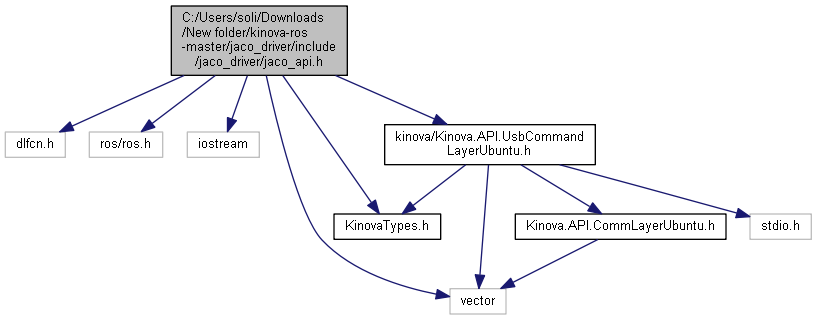
\includegraphics[width=350pt]{d1/db7/jaco__api_8h__incl}
\end{center}
\end{figure}
This graph shows which files directly or indirectly include this file\+:
\nopagebreak
\begin{figure}[H]
\begin{center}
\leavevmode
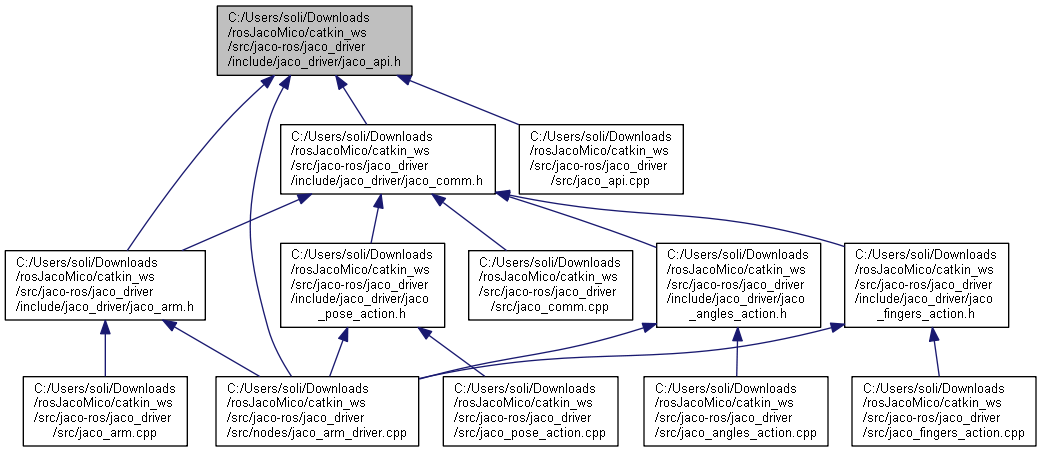
\includegraphics[width=350pt]{d0/d16/jaco__api_8h__dep__incl}
\end{center}
\end{figure}
\subsection*{Classes}
\begin{DoxyCompactItemize}
\item 
class \hyperlink{classjaco_1_1JacoAPI}{jaco\+::\+Jaco\+A\+PI}
\end{DoxyCompactItemize}
\subsection*{Namespaces}
\begin{DoxyCompactItemize}
\item 
 \hyperlink{namespacejaco}{jaco}
\end{DoxyCompactItemize}
\subsection*{Macros}
\begin{DoxyCompactItemize}
\item 
\#define \hyperlink{jaco__api_8h_aaaae826d3bd581061d04edd16b17117e}{J\+A\+C\+O\+\_\+\+U\+S\+B\+\_\+\+L\+I\+B\+R\+A\+RY}~\char`\"{}Kinova.\+A\+P\+I.\+U\+S\+B\+Command\+Layer\+Ubuntu.\+so\char`\"{}
\end{DoxyCompactItemize}


\subsection{Macro Definition Documentation}
\index{jaco\+\_\+api.\+h@{jaco\+\_\+api.\+h}!J\+A\+C\+O\+\_\+\+U\+S\+B\+\_\+\+L\+I\+B\+R\+A\+RY@{J\+A\+C\+O\+\_\+\+U\+S\+B\+\_\+\+L\+I\+B\+R\+A\+RY}}
\index{J\+A\+C\+O\+\_\+\+U\+S\+B\+\_\+\+L\+I\+B\+R\+A\+RY@{J\+A\+C\+O\+\_\+\+U\+S\+B\+\_\+\+L\+I\+B\+R\+A\+RY}!jaco\+\_\+api.\+h@{jaco\+\_\+api.\+h}}
\subsubsection[{\texorpdfstring{J\+A\+C\+O\+\_\+\+U\+S\+B\+\_\+\+L\+I\+B\+R\+A\+RY}{JACO_USB_LIBRARY}}]{\setlength{\rightskip}{0pt plus 5cm}\#define J\+A\+C\+O\+\_\+\+U\+S\+B\+\_\+\+L\+I\+B\+R\+A\+RY~\char`\"{}Kinova.\+A\+P\+I.\+U\+S\+B\+Command\+Layer\+Ubuntu.\+so\char`\"{}}\hypertarget{jaco__api_8h_aaaae826d3bd581061d04edd16b17117e}{}\label{jaco__api_8h_aaaae826d3bd581061d04edd16b17117e}

\hypertarget{jaco__arm_8h}{}\section{C\+:/\+Users/soli/\+Downloads/\+New folder/kinova-\/ros-\/master/jaco\+\_\+driver/include/jaco\+\_\+driver/jaco\+\_\+arm.h File Reference}
\label{jaco__arm_8h}\index{C\+:/\+Users/soli/\+Downloads/\+New folder/kinova-\/ros-\/master/jaco\+\_\+driver/include/jaco\+\_\+driver/jaco\+\_\+arm.\+h@{C\+:/\+Users/soli/\+Downloads/\+New folder/kinova-\/ros-\/master/jaco\+\_\+driver/include/jaco\+\_\+driver/jaco\+\_\+arm.\+h}}
{\ttfamily \#include $<$ros/ros.\+h$>$}\\*
{\ttfamily \#include $<$geometry\+\_\+msgs/\+Pose\+Stamped.\+h$>$}\\*
{\ttfamily \#include $<$geometry\+\_\+msgs/\+Wrench\+Stamped.\+h$>$}\\*
{\ttfamily \#include $<$geometry\+\_\+msgs/\+Twist\+Stamped.\+h$>$}\\*
{\ttfamily \#include $<$tf/tf.\+h$>$}\\*
{\ttfamily \#include $<$tf/transform\+\_\+listener.\+h$>$}\\*
{\ttfamily \#include $<$sensor\+\_\+msgs/\+Joint\+State.\+h$>$}\\*
{\ttfamily \#include $<$jaco\+\_\+msgs/\+Stop.\+h$>$}\\*
{\ttfamily \#include $<$jaco\+\_\+msgs/\+Start.\+h$>$}\\*
{\ttfamily \#include $<$jaco\+\_\+msgs/\+Home\+Arm.\+h$>$}\\*
{\ttfamily \#include $<$jaco\+\_\+msgs/\+Joint\+Velocity.\+h$>$}\\*
{\ttfamily \#include $<$jaco\+\_\+msgs/\+Finger\+Position.\+h$>$}\\*
{\ttfamily \#include $<$jaco\+\_\+msgs/\+Joint\+Angles.\+h$>$}\\*
{\ttfamily \#include $<$jaco\+\_\+msgs/\+Set\+Force\+Control\+Params.\+h$>$}\\*
{\ttfamily \#include $<$time.\+h$>$}\\*
{\ttfamily \#include $<$math.\+h$>$}\\*
{\ttfamily \#include $<$vector$>$}\\*
{\ttfamily \#include \char`\"{}kinova/\+Kinova\+Types.\+h\char`\"{}}\\*
{\ttfamily \#include \char`\"{}jaco\+\_\+driver/jaco\+\_\+comm.\+h\char`\"{}}\\*
{\ttfamily \#include \char`\"{}jaco\+\_\+driver/jaco\+\_\+api.\+h\char`\"{}}\\*
Include dependency graph for jaco\+\_\+arm.\+h\+:
% FIG 0
This graph shows which files directly or indirectly include this file\+:
% FIG 1
\subsection*{Classes}
\begin{DoxyCompactItemize}
\item 
class \hyperlink{classjaco_1_1_jaco_arm}{jaco\+::\+Jaco\+Arm}
\end{DoxyCompactItemize}
\subsection*{Namespaces}
\begin{DoxyCompactItemize}
\item 
 \hyperlink{namespacejaco}{jaco}
\end{DoxyCompactItemize}

\hypertarget{jaco__arm__kinematics_8h}{}\section{C\+:/\+Users/soli/\+Downloads/\+New folder/kinova-\/ros-\/master/jaco\+\_\+driver/include/jaco\+\_\+driver/jaco\+\_\+arm\+\_\+kinematics.h File Reference}
\label{jaco__arm__kinematics_8h}\index{C\+:/\+Users/soli/\+Downloads/\+New folder/kinova-\/ros-\/master/jaco\+\_\+driver/include/jaco\+\_\+driver/jaco\+\_\+arm\+\_\+kinematics.\+h@{C\+:/\+Users/soli/\+Downloads/\+New folder/kinova-\/ros-\/master/jaco\+\_\+driver/include/jaco\+\_\+driver/jaco\+\_\+arm\+\_\+kinematics.\+h}}
{\ttfamily \#include $<$math.\+h$>$}\\*
{\ttfamily \#include $<$ros/ros.\+h$>$}\\*
{\ttfamily \#include $<$tf/tf.\+h$>$}\\*
{\ttfamily \#include $<$tf/transform\+\_\+broadcaster.\+h$>$}\\*
{\ttfamily \#include $<$string$>$}\\*
Include dependency graph for jaco\+\_\+arm\+\_\+kinematics.\+h\+:
% FIG 0
This graph shows which files directly or indirectly include this file\+:
% FIG 1
\subsection*{Classes}
\begin{DoxyCompactItemize}
\item 
class \hyperlink{classjaco_1_1_jaco_kinematics}{jaco\+::\+Jaco\+Kinematics}
\end{DoxyCompactItemize}
\subsection*{Namespaces}
\begin{DoxyCompactItemize}
\item 
 \hyperlink{namespacejaco}{jaco}
\end{DoxyCompactItemize}

\hypertarget{jaco__comm_8h}{}\section{D\+:/\+Longfei/\+Desktop/catkin\+\_\+\+Kinova\+R\+O\+S/src/jaco-\/ros/jaco\+\_\+driver/include/jaco\+\_\+driver/jaco\+\_\+comm.h File Reference}
\label{jaco__comm_8h}\index{D\+:/\+Longfei/\+Desktop/catkin\+\_\+\+Kinova\+R\+O\+S/src/jaco-\/ros/jaco\+\_\+driver/include/jaco\+\_\+driver/jaco\+\_\+comm.\+h@{D\+:/\+Longfei/\+Desktop/catkin\+\_\+\+Kinova\+R\+O\+S/src/jaco-\/ros/jaco\+\_\+driver/include/jaco\+\_\+driver/jaco\+\_\+comm.\+h}}
{\ttfamily \#include $<$boost/thread/recursive\+\_\+mutex.\+hpp$>$}\\*
{\ttfamily \#include $<$kinova/\+Kinova\+Types.\+h$>$}\\*
{\ttfamily \#include $<$jaco\+\_\+driver/jaco\+\_\+types.\+h$>$}\\*
{\ttfamily \#include \char`\"{}jaco\+\_\+driver/jaco\+\_\+api.\+h\char`\"{}}\\*
Include dependency graph for jaco\+\_\+comm.\+h\+:
\nopagebreak
\begin{figure}[H]
\begin{center}
\leavevmode
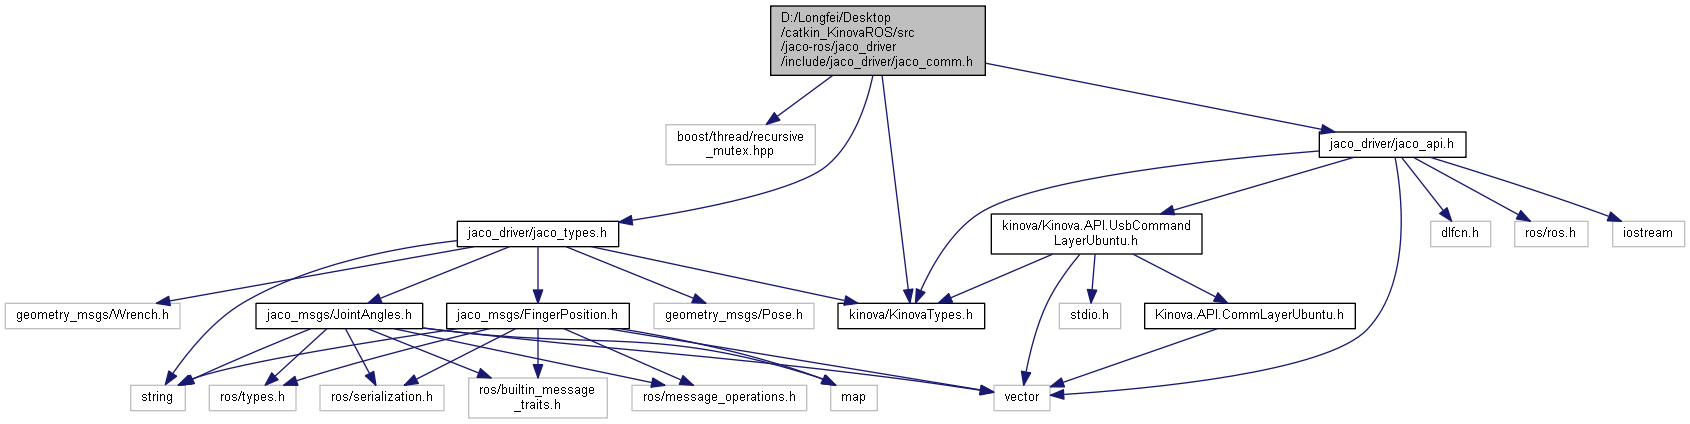
\includegraphics[width=350pt]{d9/d82/jaco__comm_8h__incl}
\end{center}
\end{figure}
This graph shows which files directly or indirectly include this file\+:
\nopagebreak
\begin{figure}[H]
\begin{center}
\leavevmode
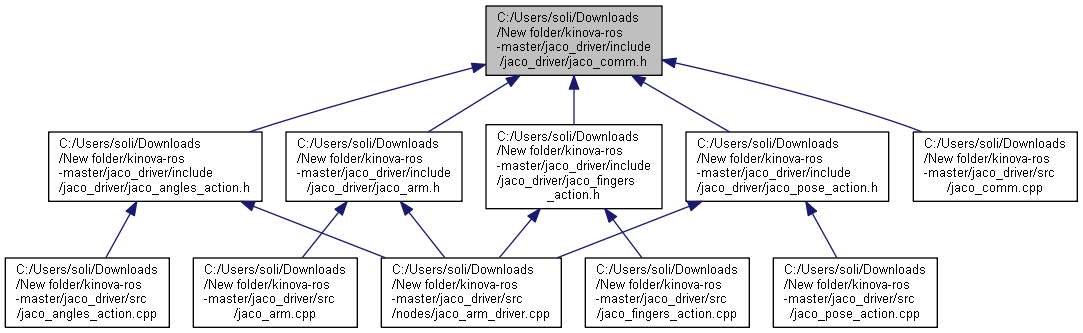
\includegraphics[width=350pt]{d3/d80/jaco__comm_8h__dep__incl}
\end{center}
\end{figure}
\subsection*{Classes}
\begin{DoxyCompactItemize}
\item 
class \hyperlink{classjaco_1_1JacoComm}{jaco\+::\+Jaco\+Comm}
\end{DoxyCompactItemize}
\subsection*{Namespaces}
\begin{DoxyCompactItemize}
\item 
 \hyperlink{namespacejaco}{jaco}
\end{DoxyCompactItemize}

\hypertarget{jaco__fingers__action_8h}{}\section{D\+:/\+Longfei/\+Desktop/catkin\+\_\+\+Kinova\+R\+O\+S/src/jaco-\/ros/jaco\+\_\+driver/include/jaco\+\_\+driver/jaco\+\_\+fingers\+\_\+action.h File Reference}
\label{jaco__fingers__action_8h}\index{D\+:/\+Longfei/\+Desktop/catkin\+\_\+\+Kinova\+R\+O\+S/src/jaco-\/ros/jaco\+\_\+driver/include/jaco\+\_\+driver/jaco\+\_\+fingers\+\_\+action.\+h@{D\+:/\+Longfei/\+Desktop/catkin\+\_\+\+Kinova\+R\+O\+S/src/jaco-\/ros/jaco\+\_\+driver/include/jaco\+\_\+driver/jaco\+\_\+fingers\+\_\+action.\+h}}
{\ttfamily \#include $<$ros/ros.\+h$>$}\\*
{\ttfamily \#include $<$actionlib/server/simple\+\_\+action\+\_\+server.\+h$>$}\\*
{\ttfamily \#include $<$jaco\+\_\+msgs/\+Set\+Fingers\+Position\+Action.\+h$>$}\\*
{\ttfamily \#include \char`\"{}jaco\+\_\+driver/jaco\+\_\+comm.\+h\char`\"{}}\\*
Include dependency graph for jaco\+\_\+fingers\+\_\+action.\+h\+:
\nopagebreak
\begin{figure}[H]
\begin{center}
\leavevmode
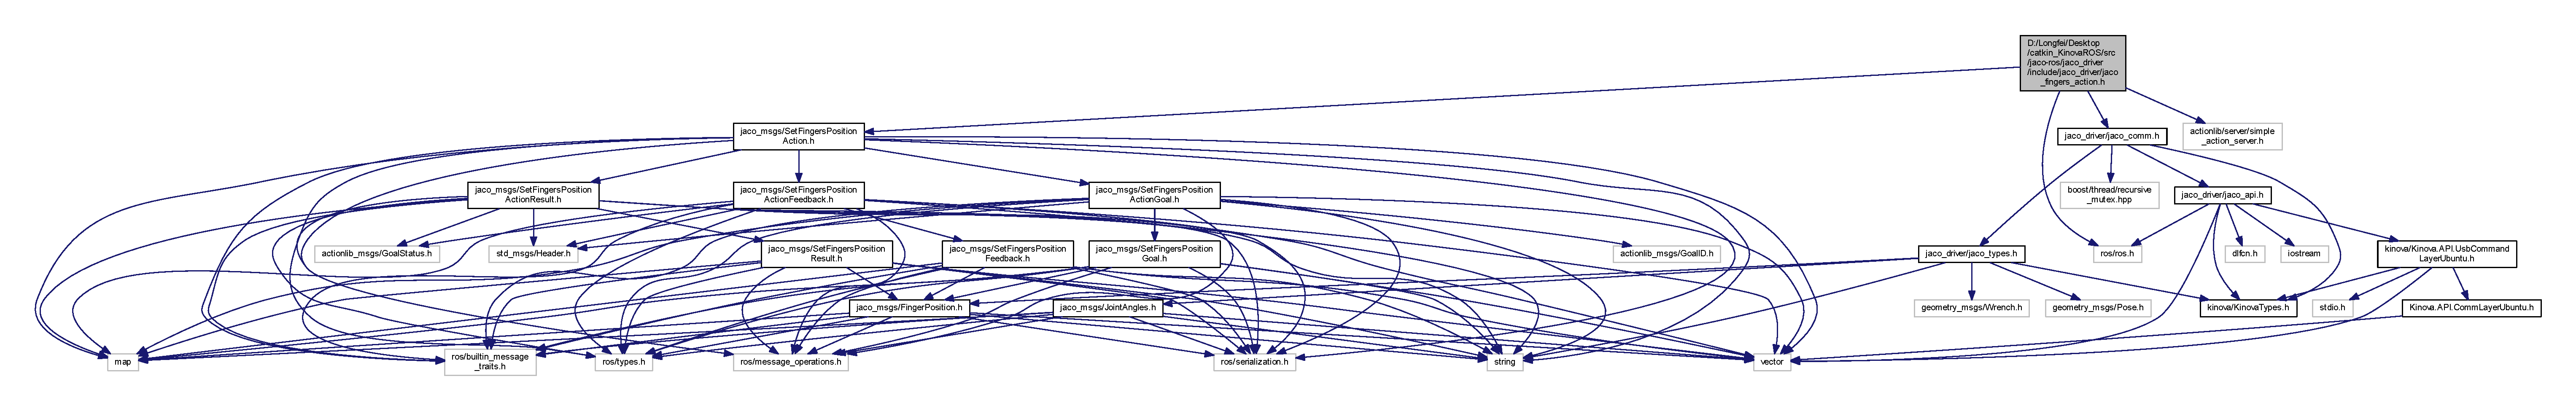
\includegraphics[width=350pt]{d2/d39/jaco__fingers__action_8h__incl}
\end{center}
\end{figure}
This graph shows which files directly or indirectly include this file\+:
\nopagebreak
\begin{figure}[H]
\begin{center}
\leavevmode
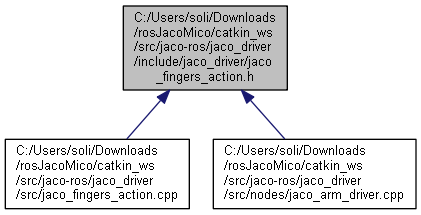
\includegraphics[width=350pt]{d5/dbb/jaco__fingers__action_8h__dep__incl}
\end{center}
\end{figure}
\subsection*{Classes}
\begin{DoxyCompactItemize}
\item 
class \hyperlink{classjaco_1_1JacoFingersActionServer}{jaco\+::\+Jaco\+Fingers\+Action\+Server}
\end{DoxyCompactItemize}
\subsection*{Namespaces}
\begin{DoxyCompactItemize}
\item 
 \hyperlink{namespacejaco}{jaco}
\end{DoxyCompactItemize}

\hypertarget{jaco__pose__action_8h}{}\section{C\+:/\+Users/soli/\+Downloads/\+New folder/kinova-\/ros-\/master/jaco\+\_\+driver/include/jaco\+\_\+driver/jaco\+\_\+pose\+\_\+action.h File Reference}
\label{jaco__pose__action_8h}\index{C\+:/\+Users/soli/\+Downloads/\+New folder/kinova-\/ros-\/master/jaco\+\_\+driver/include/jaco\+\_\+driver/jaco\+\_\+pose\+\_\+action.\+h@{C\+:/\+Users/soli/\+Downloads/\+New folder/kinova-\/ros-\/master/jaco\+\_\+driver/include/jaco\+\_\+driver/jaco\+\_\+pose\+\_\+action.\+h}}
{\ttfamily \#include $<$ros/ros.\+h$>$}\\*
{\ttfamily \#include $<$actionlib/server/simple\+\_\+action\+\_\+server.\+h$>$}\\*
{\ttfamily \#include $<$tf/tf.\+h$>$}\\*
{\ttfamily \#include $<$tf/transform\+\_\+listener.\+h$>$}\\*
{\ttfamily \#include $<$jaco\+\_\+msgs/\+Arm\+Pose\+Action.\+h$>$}\\*
{\ttfamily \#include $<$string$>$}\\*
{\ttfamily \#include \char`\"{}jaco\+\_\+driver/jaco\+\_\+comm.\+h\char`\"{}}\\*
Include dependency graph for jaco\+\_\+pose\+\_\+action.\+h\+:
% FIG 0
This graph shows which files directly or indirectly include this file\+:
% FIG 1
\subsection*{Classes}
\begin{DoxyCompactItemize}
\item 
class \hyperlink{classjaco_1_1_jaco_pose_action_server}{jaco\+::\+Jaco\+Pose\+Action\+Server}
\end{DoxyCompactItemize}
\subsection*{Namespaces}
\begin{DoxyCompactItemize}
\item 
 \hyperlink{namespacejaco}{jaco}
\end{DoxyCompactItemize}

\hypertarget{jaco__tf__updater_8h}{}\section{C\+:/\+Users/soli/\+Downloads/\+New folder/kinova-\/ros-\/master/jaco\+\_\+driver/include/jaco\+\_\+driver/jaco\+\_\+tf\+\_\+updater.h File Reference}
\label{jaco__tf__updater_8h}\index{C\+:/\+Users/soli/\+Downloads/\+New folder/kinova-\/ros-\/master/jaco\+\_\+driver/include/jaco\+\_\+driver/jaco\+\_\+tf\+\_\+updater.\+h@{C\+:/\+Users/soli/\+Downloads/\+New folder/kinova-\/ros-\/master/jaco\+\_\+driver/include/jaco\+\_\+driver/jaco\+\_\+tf\+\_\+updater.\+h}}
{\ttfamily \#include $<$time.\+h$>$}\\*
{\ttfamily \#include $<$jaco\+\_\+driver/jaco\+\_\+arm\+\_\+kinematics.\+h$>$}\\*
{\ttfamily \#include $<$ros/ros.\+h$>$}\\*
{\ttfamily \#include $<$std\+\_\+msgs/\+String.\+h$>$}\\*
{\ttfamily \#include $<$tf/tf.\+h$>$}\\*
{\ttfamily \#include $<$tf/transform\+\_\+broadcaster.\+h$>$}\\*
{\ttfamily \#include $<$tf/transform\+\_\+listener.\+h$>$}\\*
{\ttfamily \#include \char`\"{}jaco\+\_\+msgs/\+Joint\+Angles.\+h\char`\"{}}\\*
Include dependency graph for jaco\+\_\+tf\+\_\+updater.\+h\+:
% FIG 0
This graph shows which files directly or indirectly include this file\+:
% FIG 1
\subsection*{Classes}
\begin{DoxyCompactItemize}
\item 
class \hyperlink{classjaco_1_1_jaco_t_f_tree}{jaco\+::\+Jaco\+T\+F\+Tree}
\end{DoxyCompactItemize}
\subsection*{Namespaces}
\begin{DoxyCompactItemize}
\item 
 \hyperlink{namespacejaco}{jaco}
\end{DoxyCompactItemize}

\hypertarget{jaco__types_8h}{}\section{C\+:/\+Users/soli/\+Downloads/\+New folder/kinova-\/ros-\/master/jaco\+\_\+driver/include/jaco\+\_\+driver/jaco\+\_\+types.h File Reference}
\label{jaco__types_8h}\index{C\+:/\+Users/soli/\+Downloads/\+New folder/kinova-\/ros-\/master/jaco\+\_\+driver/include/jaco\+\_\+driver/jaco\+\_\+types.\+h@{C\+:/\+Users/soli/\+Downloads/\+New folder/kinova-\/ros-\/master/jaco\+\_\+driver/include/jaco\+\_\+driver/jaco\+\_\+types.\+h}}
{\ttfamily \#include $<$kinova/\+Kinova\+Types.\+h$>$}\\*
{\ttfamily \#include $<$geometry\+\_\+msgs/\+Pose.\+h$>$}\\*
{\ttfamily \#include $<$geometry\+\_\+msgs/\+Wrench.\+h$>$}\\*
{\ttfamily \#include $<$jaco\+\_\+msgs/\+Joint\+Angles.\+h$>$}\\*
{\ttfamily \#include $<$jaco\+\_\+msgs/\+Finger\+Position.\+h$>$}\\*
{\ttfamily \#include $<$string$>$}\\*
Include dependency graph for jaco\+\_\+types.\+h\+:
% FIG 0
This graph shows which files directly or indirectly include this file\+:
% FIG 1
\subsection*{Classes}
\begin{DoxyCompactItemize}
\item 
class \hyperlink{classjaco_1_1_jaco_exception}{jaco\+::\+Jaco\+Exception}
\item 
class \hyperlink{classjaco_1_1_jaco_comm_exception}{jaco\+::\+Jaco\+Comm\+Exception}
\item 
class \hyperlink{classjaco_1_1_jaco_pose}{jaco\+::\+Jaco\+Pose}
\item 
class \hyperlink{classjaco_1_1_jaco_angles}{jaco\+::\+Jaco\+Angles}
\item 
class \hyperlink{classjaco_1_1_finger_angles}{jaco\+::\+Finger\+Angles}
\end{DoxyCompactItemize}
\subsection*{Namespaces}
\begin{DoxyCompactItemize}
\item 
 \hyperlink{namespacejaco}{jaco}
\end{DoxyCompactItemize}

\hypertarget{_kinova_8_a_p_i_8_comm_layer_ubuntu_8h}{}\section{C\+:/\+Users/soli/\+Downloads/\+New folder/kinova-\/ros-\/master/jaco\+\_\+driver/include/kinova/\+Kinova.A\+P\+I.\+Comm\+Layer\+Ubuntu.\+h File Reference}
\label{_kinova_8_a_p_i_8_comm_layer_ubuntu_8h}\index{C\+:/\+Users/soli/\+Downloads/\+New folder/kinova-\/ros-\/master/jaco\+\_\+driver/include/kinova/\+Kinova.\+A\+P\+I.\+Comm\+Layer\+Ubuntu.\+h@{C\+:/\+Users/soli/\+Downloads/\+New folder/kinova-\/ros-\/master/jaco\+\_\+driver/include/kinova/\+Kinova.\+A\+P\+I.\+Comm\+Layer\+Ubuntu.\+h}}
{\ttfamily \#include $<$vector$>$}\\*
Include dependency graph for Kinova.\+A\+P\+I.\+Comm\+Layer\+Ubuntu.\+h\+:
% FIG 0
This graph shows which files directly or indirectly include this file\+:
% FIG 1
\subsection*{Classes}
\begin{DoxyCompactItemize}
\item 
struct \hyperlink{struct_packet}{Packet}
\item 
struct \hyperlink{struct_packet_list}{Packet\+List}
\item 
struct \hyperlink{struct_kinova_device}{Kinova\+Device}
\end{DoxyCompactItemize}
\subsection*{Macros}
\begin{DoxyCompactItemize}
\item 
\#define \hyperlink{_kinova_8_a_p_i_8_comm_layer_ubuntu_8h_ad200cf58a0e33b783c540d745ca27add}{K\+I\+N\+O\+V\+A\+D\+L\+L\+C\+O\+M\+M\+L\+A\+Y\+E\+R\+\_\+\+A\+PI}~\+\_\+\+\_\+declspec(dllimport)
\item 
\#define \hyperlink{_kinova_8_a_p_i_8_comm_layer_ubuntu_8h_a510f2320a2a31d2d225adc0da7bef595}{N\+O\+\_\+\+E\+R\+R\+O\+R\+\_\+\+K\+I\+N\+O\+VA}~1
\item 
\#define \hyperlink{_kinova_8_a_p_i_8_comm_layer_ubuntu_8h_af3dbe9ae36e3aa0ba20d139a987cb354}{E\+R\+R\+O\+R\+\_\+\+L\+O\+A\+D\+\_\+\+U\+S\+B\+\_\+\+L\+I\+B\+R\+A\+RY}~1001
\item 
\#define \hyperlink{_kinova_8_a_p_i_8_comm_layer_ubuntu_8h_ae16383b6f1c8166cf8ae3c4ea51f1f0b}{E\+R\+R\+O\+R\+\_\+\+O\+P\+E\+N\+\_\+\+M\+E\+T\+H\+OD}~1002
\item 
\#define \hyperlink{_kinova_8_a_p_i_8_comm_layer_ubuntu_8h_ada338ad6d3a9bc98d7ab9a91e13af88c}{E\+R\+R\+O\+R\+\_\+\+W\+R\+I\+T\+E\+\_\+\+M\+E\+T\+H\+OD}~1003
\item 
\#define \hyperlink{_kinova_8_a_p_i_8_comm_layer_ubuntu_8h_aef66c12ea6482b4c496c08a288cc7faa}{E\+R\+R\+O\+R\+\_\+\+R\+E\+A\+D\+\_\+\+M\+E\+T\+H\+OD}~1004
\item 
\#define \hyperlink{_kinova_8_a_p_i_8_comm_layer_ubuntu_8h_a0cc1d32fe6982ee696be9d1a001340fe}{E\+R\+R\+O\+R\+\_\+\+R\+E\+A\+D\+\_\+\+I\+N\+T\+\_\+\+M\+E\+T\+H\+OD}~1005
\item 
\#define \hyperlink{_kinova_8_a_p_i_8_comm_layer_ubuntu_8h_a135c6a9b1729ec2cc26109fa1011dd60}{E\+R\+R\+O\+R\+\_\+\+F\+R\+E\+E\+\_\+\+L\+I\+B\+R\+A\+RY}~1006
\item 
\#define \hyperlink{_kinova_8_a_p_i_8_comm_layer_ubuntu_8h_afd94861330305625c61219ed28b02a36}{E\+R\+R\+O\+R\+\_\+\+J\+A\+C\+O\+\_\+\+C\+O\+N\+N\+E\+C\+T\+I\+ON}~1007
\item 
\#define \hyperlink{_kinova_8_a_p_i_8_comm_layer_ubuntu_8h_a8bef7198cac5a66787097490eb9289a6}{E\+R\+R\+O\+R\+\_\+\+C\+L\+A\+I\+M\+\_\+\+I\+N\+T\+E\+R\+F\+A\+CE}~1008
\item 
\#define \hyperlink{_kinova_8_a_p_i_8_comm_layer_ubuntu_8h_ad8ff335f164c59e9ea2f9f500fb81c50}{E\+R\+R\+O\+R\+\_\+\+U\+N\+K\+N\+O\+W\+N\+\_\+\+D\+E\+V\+I\+CE}~1009
\item 
\#define \hyperlink{_kinova_8_a_p_i_8_comm_layer_ubuntu_8h_a605e0ff46555922872461535eca0d0b9}{E\+R\+R\+O\+R\+\_\+\+N\+O\+T\+\_\+\+I\+N\+I\+T\+I\+A\+L\+I\+Z\+ED}~1010
\item 
\#define \hyperlink{_kinova_8_a_p_i_8_comm_layer_ubuntu_8h_ad42ee2931c53f250d85555f35bb8ee81}{E\+R\+R\+O\+R\+\_\+\+L\+I\+B\+U\+S\+B\+\_\+\+N\+O\+\_\+\+D\+E\+V\+I\+CE}~1011
\item 
\#define \hyperlink{_kinova_8_a_p_i_8_comm_layer_ubuntu_8h_ac990045d67e6561d7cddb33a9484e48c}{E\+R\+R\+O\+R\+\_\+\+L\+I\+B\+U\+S\+B\+\_\+\+B\+U\+SY}~1012
\item 
\#define \hyperlink{_kinova_8_a_p_i_8_comm_layer_ubuntu_8h_af88b346701ceadbdd6fc3d8ca1f4befe}{E\+R\+R\+O\+R\+\_\+\+L\+I\+B\+U\+S\+B\+\_\+\+N\+O\+T\+\_\+\+S\+U\+P\+P\+O\+R\+T\+ED}~1013
\item 
\#define \hyperlink{_kinova_8_a_p_i_8_comm_layer_ubuntu_8h_a46ec259f48cc0f825cec63da32c2d640}{E\+R\+R\+O\+R\+\_\+\+S\+E\+N\+D\+P\+A\+C\+K\+E\+T\+\_\+\+U\+N\+K\+N\+O\+WN}~1014
\item 
\#define \hyperlink{_kinova_8_a_p_i_8_comm_layer_ubuntu_8h_ad6dae5cdf107e5b57dc4e13427c608b7}{E\+R\+R\+O\+R\+\_\+\+N\+O\+\_\+\+D\+E\+V\+I\+C\+E\+\_\+\+F\+O\+U\+ND}~1015
\item 
\#define \hyperlink{_kinova_8_a_p_i_8_comm_layer_ubuntu_8h_aebdc7d8ca8e25ed8efc90bb88ef7ef5b}{P\+A\+C\+K\+E\+T\+\_\+\+S\+I\+ZE}~64
\item 
\#define \hyperlink{_kinova_8_a_p_i_8_comm_layer_ubuntu_8h_a515f46a87f301d94d9f3b06a6bb2540a}{P\+A\+C\+K\+E\+T\+\_\+\+D\+A\+T\+A\+\_\+\+S\+I\+ZE}~56
\item 
\#define \hyperlink{_kinova_8_a_p_i_8_comm_layer_ubuntu_8h_a69bfb6e73bae0625ac56f441ccf542d1}{P\+A\+C\+K\+E\+T\+\_\+\+H\+E\+A\+D\+E\+R\+\_\+\+S\+I\+ZE}~8
\item 
\#define \hyperlink{_kinova_8_a_p_i_8_comm_layer_ubuntu_8h_a2e19fae8619e7a3b28aecdcf5d7cd51d}{S\+E\+R\+I\+A\+L\+\_\+\+L\+E\+N\+G\+TH}~20
\end{DoxyCompactItemize}
\subsection*{Functions}
\begin{DoxyCompactItemize}
\item 
\hyperlink{_kinova_8_a_p_i_8_comm_layer_ubuntu_8h_a1d3678de7e45bc92e4c8ee7ece40c833}{\+\_\+\+\_\+attribute\+\_\+\+\_\+} ((visibility(\char`\"{}default\char`\"{}))) int Init\+Communication(void)
\end{DoxyCompactItemize}
\subsection*{Variables}
\begin{DoxyCompactItemize}
\item 
\hyperlink{struct_packet}{Packet} \& \hyperlink{_kinova_8_a_p_i_8_comm_layer_ubuntu_8h_a0929bb1a4a68ea14e4871a32a70d7fa6}{packet\+In}
\item 
\hyperlink{struct_packet}{Packet} int \& \hyperlink{_kinova_8_a_p_i_8_comm_layer_ubuntu_8h_a900dac90961bada00f57c207562a6a9a}{result}
\end{DoxyCompactItemize}


\subsection{Macro Definition Documentation}
\index{Kinova.\+A\+P\+I.\+Comm\+Layer\+Ubuntu.\+h@{Kinova.\+A\+P\+I.\+Comm\+Layer\+Ubuntu.\+h}!E\+R\+R\+O\+R\+\_\+\+C\+L\+A\+I\+M\+\_\+\+I\+N\+T\+E\+R\+F\+A\+CE@{E\+R\+R\+O\+R\+\_\+\+C\+L\+A\+I\+M\+\_\+\+I\+N\+T\+E\+R\+F\+A\+CE}}
\index{E\+R\+R\+O\+R\+\_\+\+C\+L\+A\+I\+M\+\_\+\+I\+N\+T\+E\+R\+F\+A\+CE@{E\+R\+R\+O\+R\+\_\+\+C\+L\+A\+I\+M\+\_\+\+I\+N\+T\+E\+R\+F\+A\+CE}!Kinova.\+A\+P\+I.\+Comm\+Layer\+Ubuntu.\+h@{Kinova.\+A\+P\+I.\+Comm\+Layer\+Ubuntu.\+h}}
\subsubsection[{\texorpdfstring{E\+R\+R\+O\+R\+\_\+\+C\+L\+A\+I\+M\+\_\+\+I\+N\+T\+E\+R\+F\+A\+CE}{ERROR_CLAIM_INTERFACE}}]{\setlength{\rightskip}{0pt plus 5cm}\#define E\+R\+R\+O\+R\+\_\+\+C\+L\+A\+I\+M\+\_\+\+I\+N\+T\+E\+R\+F\+A\+CE~1008}\hypertarget{_kinova_8_a_p_i_8_comm_layer_ubuntu_8h_a8bef7198cac5a66787097490eb9289a6}{}\label{_kinova_8_a_p_i_8_comm_layer_ubuntu_8h_a8bef7198cac5a66787097490eb9289a6}
\index{Kinova.\+A\+P\+I.\+Comm\+Layer\+Ubuntu.\+h@{Kinova.\+A\+P\+I.\+Comm\+Layer\+Ubuntu.\+h}!E\+R\+R\+O\+R\+\_\+\+F\+R\+E\+E\+\_\+\+L\+I\+B\+R\+A\+RY@{E\+R\+R\+O\+R\+\_\+\+F\+R\+E\+E\+\_\+\+L\+I\+B\+R\+A\+RY}}
\index{E\+R\+R\+O\+R\+\_\+\+F\+R\+E\+E\+\_\+\+L\+I\+B\+R\+A\+RY@{E\+R\+R\+O\+R\+\_\+\+F\+R\+E\+E\+\_\+\+L\+I\+B\+R\+A\+RY}!Kinova.\+A\+P\+I.\+Comm\+Layer\+Ubuntu.\+h@{Kinova.\+A\+P\+I.\+Comm\+Layer\+Ubuntu.\+h}}
\subsubsection[{\texorpdfstring{E\+R\+R\+O\+R\+\_\+\+F\+R\+E\+E\+\_\+\+L\+I\+B\+R\+A\+RY}{ERROR_FREE_LIBRARY}}]{\setlength{\rightskip}{0pt plus 5cm}\#define E\+R\+R\+O\+R\+\_\+\+F\+R\+E\+E\+\_\+\+L\+I\+B\+R\+A\+RY~1006}\hypertarget{_kinova_8_a_p_i_8_comm_layer_ubuntu_8h_a135c6a9b1729ec2cc26109fa1011dd60}{}\label{_kinova_8_a_p_i_8_comm_layer_ubuntu_8h_a135c6a9b1729ec2cc26109fa1011dd60}
\index{Kinova.\+A\+P\+I.\+Comm\+Layer\+Ubuntu.\+h@{Kinova.\+A\+P\+I.\+Comm\+Layer\+Ubuntu.\+h}!E\+R\+R\+O\+R\+\_\+\+J\+A\+C\+O\+\_\+\+C\+O\+N\+N\+E\+C\+T\+I\+ON@{E\+R\+R\+O\+R\+\_\+\+J\+A\+C\+O\+\_\+\+C\+O\+N\+N\+E\+C\+T\+I\+ON}}
\index{E\+R\+R\+O\+R\+\_\+\+J\+A\+C\+O\+\_\+\+C\+O\+N\+N\+E\+C\+T\+I\+ON@{E\+R\+R\+O\+R\+\_\+\+J\+A\+C\+O\+\_\+\+C\+O\+N\+N\+E\+C\+T\+I\+ON}!Kinova.\+A\+P\+I.\+Comm\+Layer\+Ubuntu.\+h@{Kinova.\+A\+P\+I.\+Comm\+Layer\+Ubuntu.\+h}}
\subsubsection[{\texorpdfstring{E\+R\+R\+O\+R\+\_\+\+J\+A\+C\+O\+\_\+\+C\+O\+N\+N\+E\+C\+T\+I\+ON}{ERROR_JACO_CONNECTION}}]{\setlength{\rightskip}{0pt plus 5cm}\#define E\+R\+R\+O\+R\+\_\+\+J\+A\+C\+O\+\_\+\+C\+O\+N\+N\+E\+C\+T\+I\+ON~1007}\hypertarget{_kinova_8_a_p_i_8_comm_layer_ubuntu_8h_afd94861330305625c61219ed28b02a36}{}\label{_kinova_8_a_p_i_8_comm_layer_ubuntu_8h_afd94861330305625c61219ed28b02a36}
\index{Kinova.\+A\+P\+I.\+Comm\+Layer\+Ubuntu.\+h@{Kinova.\+A\+P\+I.\+Comm\+Layer\+Ubuntu.\+h}!E\+R\+R\+O\+R\+\_\+\+L\+I\+B\+U\+S\+B\+\_\+\+B\+U\+SY@{E\+R\+R\+O\+R\+\_\+\+L\+I\+B\+U\+S\+B\+\_\+\+B\+U\+SY}}
\index{E\+R\+R\+O\+R\+\_\+\+L\+I\+B\+U\+S\+B\+\_\+\+B\+U\+SY@{E\+R\+R\+O\+R\+\_\+\+L\+I\+B\+U\+S\+B\+\_\+\+B\+U\+SY}!Kinova.\+A\+P\+I.\+Comm\+Layer\+Ubuntu.\+h@{Kinova.\+A\+P\+I.\+Comm\+Layer\+Ubuntu.\+h}}
\subsubsection[{\texorpdfstring{E\+R\+R\+O\+R\+\_\+\+L\+I\+B\+U\+S\+B\+\_\+\+B\+U\+SY}{ERROR_LIBUSB_BUSY}}]{\setlength{\rightskip}{0pt plus 5cm}\#define E\+R\+R\+O\+R\+\_\+\+L\+I\+B\+U\+S\+B\+\_\+\+B\+U\+SY~1012}\hypertarget{_kinova_8_a_p_i_8_comm_layer_ubuntu_8h_ac990045d67e6561d7cddb33a9484e48c}{}\label{_kinova_8_a_p_i_8_comm_layer_ubuntu_8h_ac990045d67e6561d7cddb33a9484e48c}
\index{Kinova.\+A\+P\+I.\+Comm\+Layer\+Ubuntu.\+h@{Kinova.\+A\+P\+I.\+Comm\+Layer\+Ubuntu.\+h}!E\+R\+R\+O\+R\+\_\+\+L\+I\+B\+U\+S\+B\+\_\+\+N\+O\+\_\+\+D\+E\+V\+I\+CE@{E\+R\+R\+O\+R\+\_\+\+L\+I\+B\+U\+S\+B\+\_\+\+N\+O\+\_\+\+D\+E\+V\+I\+CE}}
\index{E\+R\+R\+O\+R\+\_\+\+L\+I\+B\+U\+S\+B\+\_\+\+N\+O\+\_\+\+D\+E\+V\+I\+CE@{E\+R\+R\+O\+R\+\_\+\+L\+I\+B\+U\+S\+B\+\_\+\+N\+O\+\_\+\+D\+E\+V\+I\+CE}!Kinova.\+A\+P\+I.\+Comm\+Layer\+Ubuntu.\+h@{Kinova.\+A\+P\+I.\+Comm\+Layer\+Ubuntu.\+h}}
\subsubsection[{\texorpdfstring{E\+R\+R\+O\+R\+\_\+\+L\+I\+B\+U\+S\+B\+\_\+\+N\+O\+\_\+\+D\+E\+V\+I\+CE}{ERROR_LIBUSB_NO_DEVICE}}]{\setlength{\rightskip}{0pt plus 5cm}\#define E\+R\+R\+O\+R\+\_\+\+L\+I\+B\+U\+S\+B\+\_\+\+N\+O\+\_\+\+D\+E\+V\+I\+CE~1011}\hypertarget{_kinova_8_a_p_i_8_comm_layer_ubuntu_8h_ad42ee2931c53f250d85555f35bb8ee81}{}\label{_kinova_8_a_p_i_8_comm_layer_ubuntu_8h_ad42ee2931c53f250d85555f35bb8ee81}
\index{Kinova.\+A\+P\+I.\+Comm\+Layer\+Ubuntu.\+h@{Kinova.\+A\+P\+I.\+Comm\+Layer\+Ubuntu.\+h}!E\+R\+R\+O\+R\+\_\+\+L\+I\+B\+U\+S\+B\+\_\+\+N\+O\+T\+\_\+\+S\+U\+P\+P\+O\+R\+T\+ED@{E\+R\+R\+O\+R\+\_\+\+L\+I\+B\+U\+S\+B\+\_\+\+N\+O\+T\+\_\+\+S\+U\+P\+P\+O\+R\+T\+ED}}
\index{E\+R\+R\+O\+R\+\_\+\+L\+I\+B\+U\+S\+B\+\_\+\+N\+O\+T\+\_\+\+S\+U\+P\+P\+O\+R\+T\+ED@{E\+R\+R\+O\+R\+\_\+\+L\+I\+B\+U\+S\+B\+\_\+\+N\+O\+T\+\_\+\+S\+U\+P\+P\+O\+R\+T\+ED}!Kinova.\+A\+P\+I.\+Comm\+Layer\+Ubuntu.\+h@{Kinova.\+A\+P\+I.\+Comm\+Layer\+Ubuntu.\+h}}
\subsubsection[{\texorpdfstring{E\+R\+R\+O\+R\+\_\+\+L\+I\+B\+U\+S\+B\+\_\+\+N\+O\+T\+\_\+\+S\+U\+P\+P\+O\+R\+T\+ED}{ERROR_LIBUSB_NOT_SUPPORTED}}]{\setlength{\rightskip}{0pt plus 5cm}\#define E\+R\+R\+O\+R\+\_\+\+L\+I\+B\+U\+S\+B\+\_\+\+N\+O\+T\+\_\+\+S\+U\+P\+P\+O\+R\+T\+ED~1013}\hypertarget{_kinova_8_a_p_i_8_comm_layer_ubuntu_8h_af88b346701ceadbdd6fc3d8ca1f4befe}{}\label{_kinova_8_a_p_i_8_comm_layer_ubuntu_8h_af88b346701ceadbdd6fc3d8ca1f4befe}
\index{Kinova.\+A\+P\+I.\+Comm\+Layer\+Ubuntu.\+h@{Kinova.\+A\+P\+I.\+Comm\+Layer\+Ubuntu.\+h}!E\+R\+R\+O\+R\+\_\+\+L\+O\+A\+D\+\_\+\+U\+S\+B\+\_\+\+L\+I\+B\+R\+A\+RY@{E\+R\+R\+O\+R\+\_\+\+L\+O\+A\+D\+\_\+\+U\+S\+B\+\_\+\+L\+I\+B\+R\+A\+RY}}
\index{E\+R\+R\+O\+R\+\_\+\+L\+O\+A\+D\+\_\+\+U\+S\+B\+\_\+\+L\+I\+B\+R\+A\+RY@{E\+R\+R\+O\+R\+\_\+\+L\+O\+A\+D\+\_\+\+U\+S\+B\+\_\+\+L\+I\+B\+R\+A\+RY}!Kinova.\+A\+P\+I.\+Comm\+Layer\+Ubuntu.\+h@{Kinova.\+A\+P\+I.\+Comm\+Layer\+Ubuntu.\+h}}
\subsubsection[{\texorpdfstring{E\+R\+R\+O\+R\+\_\+\+L\+O\+A\+D\+\_\+\+U\+S\+B\+\_\+\+L\+I\+B\+R\+A\+RY}{ERROR_LOAD_USB_LIBRARY}}]{\setlength{\rightskip}{0pt plus 5cm}\#define E\+R\+R\+O\+R\+\_\+\+L\+O\+A\+D\+\_\+\+U\+S\+B\+\_\+\+L\+I\+B\+R\+A\+RY~1001}\hypertarget{_kinova_8_a_p_i_8_comm_layer_ubuntu_8h_af3dbe9ae36e3aa0ba20d139a987cb354}{}\label{_kinova_8_a_p_i_8_comm_layer_ubuntu_8h_af3dbe9ae36e3aa0ba20d139a987cb354}
\index{Kinova.\+A\+P\+I.\+Comm\+Layer\+Ubuntu.\+h@{Kinova.\+A\+P\+I.\+Comm\+Layer\+Ubuntu.\+h}!E\+R\+R\+O\+R\+\_\+\+N\+O\+\_\+\+D\+E\+V\+I\+C\+E\+\_\+\+F\+O\+U\+ND@{E\+R\+R\+O\+R\+\_\+\+N\+O\+\_\+\+D\+E\+V\+I\+C\+E\+\_\+\+F\+O\+U\+ND}}
\index{E\+R\+R\+O\+R\+\_\+\+N\+O\+\_\+\+D\+E\+V\+I\+C\+E\+\_\+\+F\+O\+U\+ND@{E\+R\+R\+O\+R\+\_\+\+N\+O\+\_\+\+D\+E\+V\+I\+C\+E\+\_\+\+F\+O\+U\+ND}!Kinova.\+A\+P\+I.\+Comm\+Layer\+Ubuntu.\+h@{Kinova.\+A\+P\+I.\+Comm\+Layer\+Ubuntu.\+h}}
\subsubsection[{\texorpdfstring{E\+R\+R\+O\+R\+\_\+\+N\+O\+\_\+\+D\+E\+V\+I\+C\+E\+\_\+\+F\+O\+U\+ND}{ERROR_NO_DEVICE_FOUND}}]{\setlength{\rightskip}{0pt plus 5cm}\#define E\+R\+R\+O\+R\+\_\+\+N\+O\+\_\+\+D\+E\+V\+I\+C\+E\+\_\+\+F\+O\+U\+ND~1015}\hypertarget{_kinova_8_a_p_i_8_comm_layer_ubuntu_8h_ad6dae5cdf107e5b57dc4e13427c608b7}{}\label{_kinova_8_a_p_i_8_comm_layer_ubuntu_8h_ad6dae5cdf107e5b57dc4e13427c608b7}
\index{Kinova.\+A\+P\+I.\+Comm\+Layer\+Ubuntu.\+h@{Kinova.\+A\+P\+I.\+Comm\+Layer\+Ubuntu.\+h}!E\+R\+R\+O\+R\+\_\+\+N\+O\+T\+\_\+\+I\+N\+I\+T\+I\+A\+L\+I\+Z\+ED@{E\+R\+R\+O\+R\+\_\+\+N\+O\+T\+\_\+\+I\+N\+I\+T\+I\+A\+L\+I\+Z\+ED}}
\index{E\+R\+R\+O\+R\+\_\+\+N\+O\+T\+\_\+\+I\+N\+I\+T\+I\+A\+L\+I\+Z\+ED@{E\+R\+R\+O\+R\+\_\+\+N\+O\+T\+\_\+\+I\+N\+I\+T\+I\+A\+L\+I\+Z\+ED}!Kinova.\+A\+P\+I.\+Comm\+Layer\+Ubuntu.\+h@{Kinova.\+A\+P\+I.\+Comm\+Layer\+Ubuntu.\+h}}
\subsubsection[{\texorpdfstring{E\+R\+R\+O\+R\+\_\+\+N\+O\+T\+\_\+\+I\+N\+I\+T\+I\+A\+L\+I\+Z\+ED}{ERROR_NOT_INITIALIZED}}]{\setlength{\rightskip}{0pt plus 5cm}\#define E\+R\+R\+O\+R\+\_\+\+N\+O\+T\+\_\+\+I\+N\+I\+T\+I\+A\+L\+I\+Z\+ED~1010}\hypertarget{_kinova_8_a_p_i_8_comm_layer_ubuntu_8h_a605e0ff46555922872461535eca0d0b9}{}\label{_kinova_8_a_p_i_8_comm_layer_ubuntu_8h_a605e0ff46555922872461535eca0d0b9}
\index{Kinova.\+A\+P\+I.\+Comm\+Layer\+Ubuntu.\+h@{Kinova.\+A\+P\+I.\+Comm\+Layer\+Ubuntu.\+h}!E\+R\+R\+O\+R\+\_\+\+O\+P\+E\+N\+\_\+\+M\+E\+T\+H\+OD@{E\+R\+R\+O\+R\+\_\+\+O\+P\+E\+N\+\_\+\+M\+E\+T\+H\+OD}}
\index{E\+R\+R\+O\+R\+\_\+\+O\+P\+E\+N\+\_\+\+M\+E\+T\+H\+OD@{E\+R\+R\+O\+R\+\_\+\+O\+P\+E\+N\+\_\+\+M\+E\+T\+H\+OD}!Kinova.\+A\+P\+I.\+Comm\+Layer\+Ubuntu.\+h@{Kinova.\+A\+P\+I.\+Comm\+Layer\+Ubuntu.\+h}}
\subsubsection[{\texorpdfstring{E\+R\+R\+O\+R\+\_\+\+O\+P\+E\+N\+\_\+\+M\+E\+T\+H\+OD}{ERROR_OPEN_METHOD}}]{\setlength{\rightskip}{0pt plus 5cm}\#define E\+R\+R\+O\+R\+\_\+\+O\+P\+E\+N\+\_\+\+M\+E\+T\+H\+OD~1002}\hypertarget{_kinova_8_a_p_i_8_comm_layer_ubuntu_8h_ae16383b6f1c8166cf8ae3c4ea51f1f0b}{}\label{_kinova_8_a_p_i_8_comm_layer_ubuntu_8h_ae16383b6f1c8166cf8ae3c4ea51f1f0b}
\index{Kinova.\+A\+P\+I.\+Comm\+Layer\+Ubuntu.\+h@{Kinova.\+A\+P\+I.\+Comm\+Layer\+Ubuntu.\+h}!E\+R\+R\+O\+R\+\_\+\+R\+E\+A\+D\+\_\+\+I\+N\+T\+\_\+\+M\+E\+T\+H\+OD@{E\+R\+R\+O\+R\+\_\+\+R\+E\+A\+D\+\_\+\+I\+N\+T\+\_\+\+M\+E\+T\+H\+OD}}
\index{E\+R\+R\+O\+R\+\_\+\+R\+E\+A\+D\+\_\+\+I\+N\+T\+\_\+\+M\+E\+T\+H\+OD@{E\+R\+R\+O\+R\+\_\+\+R\+E\+A\+D\+\_\+\+I\+N\+T\+\_\+\+M\+E\+T\+H\+OD}!Kinova.\+A\+P\+I.\+Comm\+Layer\+Ubuntu.\+h@{Kinova.\+A\+P\+I.\+Comm\+Layer\+Ubuntu.\+h}}
\subsubsection[{\texorpdfstring{E\+R\+R\+O\+R\+\_\+\+R\+E\+A\+D\+\_\+\+I\+N\+T\+\_\+\+M\+E\+T\+H\+OD}{ERROR_READ_INT_METHOD}}]{\setlength{\rightskip}{0pt plus 5cm}\#define E\+R\+R\+O\+R\+\_\+\+R\+E\+A\+D\+\_\+\+I\+N\+T\+\_\+\+M\+E\+T\+H\+OD~1005}\hypertarget{_kinova_8_a_p_i_8_comm_layer_ubuntu_8h_a0cc1d32fe6982ee696be9d1a001340fe}{}\label{_kinova_8_a_p_i_8_comm_layer_ubuntu_8h_a0cc1d32fe6982ee696be9d1a001340fe}
\index{Kinova.\+A\+P\+I.\+Comm\+Layer\+Ubuntu.\+h@{Kinova.\+A\+P\+I.\+Comm\+Layer\+Ubuntu.\+h}!E\+R\+R\+O\+R\+\_\+\+R\+E\+A\+D\+\_\+\+M\+E\+T\+H\+OD@{E\+R\+R\+O\+R\+\_\+\+R\+E\+A\+D\+\_\+\+M\+E\+T\+H\+OD}}
\index{E\+R\+R\+O\+R\+\_\+\+R\+E\+A\+D\+\_\+\+M\+E\+T\+H\+OD@{E\+R\+R\+O\+R\+\_\+\+R\+E\+A\+D\+\_\+\+M\+E\+T\+H\+OD}!Kinova.\+A\+P\+I.\+Comm\+Layer\+Ubuntu.\+h@{Kinova.\+A\+P\+I.\+Comm\+Layer\+Ubuntu.\+h}}
\subsubsection[{\texorpdfstring{E\+R\+R\+O\+R\+\_\+\+R\+E\+A\+D\+\_\+\+M\+E\+T\+H\+OD}{ERROR_READ_METHOD}}]{\setlength{\rightskip}{0pt plus 5cm}\#define E\+R\+R\+O\+R\+\_\+\+R\+E\+A\+D\+\_\+\+M\+E\+T\+H\+OD~1004}\hypertarget{_kinova_8_a_p_i_8_comm_layer_ubuntu_8h_aef66c12ea6482b4c496c08a288cc7faa}{}\label{_kinova_8_a_p_i_8_comm_layer_ubuntu_8h_aef66c12ea6482b4c496c08a288cc7faa}
\index{Kinova.\+A\+P\+I.\+Comm\+Layer\+Ubuntu.\+h@{Kinova.\+A\+P\+I.\+Comm\+Layer\+Ubuntu.\+h}!E\+R\+R\+O\+R\+\_\+\+S\+E\+N\+D\+P\+A\+C\+K\+E\+T\+\_\+\+U\+N\+K\+N\+O\+WN@{E\+R\+R\+O\+R\+\_\+\+S\+E\+N\+D\+P\+A\+C\+K\+E\+T\+\_\+\+U\+N\+K\+N\+O\+WN}}
\index{E\+R\+R\+O\+R\+\_\+\+S\+E\+N\+D\+P\+A\+C\+K\+E\+T\+\_\+\+U\+N\+K\+N\+O\+WN@{E\+R\+R\+O\+R\+\_\+\+S\+E\+N\+D\+P\+A\+C\+K\+E\+T\+\_\+\+U\+N\+K\+N\+O\+WN}!Kinova.\+A\+P\+I.\+Comm\+Layer\+Ubuntu.\+h@{Kinova.\+A\+P\+I.\+Comm\+Layer\+Ubuntu.\+h}}
\subsubsection[{\texorpdfstring{E\+R\+R\+O\+R\+\_\+\+S\+E\+N\+D\+P\+A\+C\+K\+E\+T\+\_\+\+U\+N\+K\+N\+O\+WN}{ERROR_SENDPACKET_UNKNOWN}}]{\setlength{\rightskip}{0pt plus 5cm}\#define E\+R\+R\+O\+R\+\_\+\+S\+E\+N\+D\+P\+A\+C\+K\+E\+T\+\_\+\+U\+N\+K\+N\+O\+WN~1014}\hypertarget{_kinova_8_a_p_i_8_comm_layer_ubuntu_8h_a46ec259f48cc0f825cec63da32c2d640}{}\label{_kinova_8_a_p_i_8_comm_layer_ubuntu_8h_a46ec259f48cc0f825cec63da32c2d640}
\index{Kinova.\+A\+P\+I.\+Comm\+Layer\+Ubuntu.\+h@{Kinova.\+A\+P\+I.\+Comm\+Layer\+Ubuntu.\+h}!E\+R\+R\+O\+R\+\_\+\+U\+N\+K\+N\+O\+W\+N\+\_\+\+D\+E\+V\+I\+CE@{E\+R\+R\+O\+R\+\_\+\+U\+N\+K\+N\+O\+W\+N\+\_\+\+D\+E\+V\+I\+CE}}
\index{E\+R\+R\+O\+R\+\_\+\+U\+N\+K\+N\+O\+W\+N\+\_\+\+D\+E\+V\+I\+CE@{E\+R\+R\+O\+R\+\_\+\+U\+N\+K\+N\+O\+W\+N\+\_\+\+D\+E\+V\+I\+CE}!Kinova.\+A\+P\+I.\+Comm\+Layer\+Ubuntu.\+h@{Kinova.\+A\+P\+I.\+Comm\+Layer\+Ubuntu.\+h}}
\subsubsection[{\texorpdfstring{E\+R\+R\+O\+R\+\_\+\+U\+N\+K\+N\+O\+W\+N\+\_\+\+D\+E\+V\+I\+CE}{ERROR_UNKNOWN_DEVICE}}]{\setlength{\rightskip}{0pt plus 5cm}\#define E\+R\+R\+O\+R\+\_\+\+U\+N\+K\+N\+O\+W\+N\+\_\+\+D\+E\+V\+I\+CE~1009}\hypertarget{_kinova_8_a_p_i_8_comm_layer_ubuntu_8h_ad8ff335f164c59e9ea2f9f500fb81c50}{}\label{_kinova_8_a_p_i_8_comm_layer_ubuntu_8h_ad8ff335f164c59e9ea2f9f500fb81c50}
\index{Kinova.\+A\+P\+I.\+Comm\+Layer\+Ubuntu.\+h@{Kinova.\+A\+P\+I.\+Comm\+Layer\+Ubuntu.\+h}!E\+R\+R\+O\+R\+\_\+\+W\+R\+I\+T\+E\+\_\+\+M\+E\+T\+H\+OD@{E\+R\+R\+O\+R\+\_\+\+W\+R\+I\+T\+E\+\_\+\+M\+E\+T\+H\+OD}}
\index{E\+R\+R\+O\+R\+\_\+\+W\+R\+I\+T\+E\+\_\+\+M\+E\+T\+H\+OD@{E\+R\+R\+O\+R\+\_\+\+W\+R\+I\+T\+E\+\_\+\+M\+E\+T\+H\+OD}!Kinova.\+A\+P\+I.\+Comm\+Layer\+Ubuntu.\+h@{Kinova.\+A\+P\+I.\+Comm\+Layer\+Ubuntu.\+h}}
\subsubsection[{\texorpdfstring{E\+R\+R\+O\+R\+\_\+\+W\+R\+I\+T\+E\+\_\+\+M\+E\+T\+H\+OD}{ERROR_WRITE_METHOD}}]{\setlength{\rightskip}{0pt plus 5cm}\#define E\+R\+R\+O\+R\+\_\+\+W\+R\+I\+T\+E\+\_\+\+M\+E\+T\+H\+OD~1003}\hypertarget{_kinova_8_a_p_i_8_comm_layer_ubuntu_8h_ada338ad6d3a9bc98d7ab9a91e13af88c}{}\label{_kinova_8_a_p_i_8_comm_layer_ubuntu_8h_ada338ad6d3a9bc98d7ab9a91e13af88c}
\index{Kinova.\+A\+P\+I.\+Comm\+Layer\+Ubuntu.\+h@{Kinova.\+A\+P\+I.\+Comm\+Layer\+Ubuntu.\+h}!K\+I\+N\+O\+V\+A\+D\+L\+L\+C\+O\+M\+M\+L\+A\+Y\+E\+R\+\_\+\+A\+PI@{K\+I\+N\+O\+V\+A\+D\+L\+L\+C\+O\+M\+M\+L\+A\+Y\+E\+R\+\_\+\+A\+PI}}
\index{K\+I\+N\+O\+V\+A\+D\+L\+L\+C\+O\+M\+M\+L\+A\+Y\+E\+R\+\_\+\+A\+PI@{K\+I\+N\+O\+V\+A\+D\+L\+L\+C\+O\+M\+M\+L\+A\+Y\+E\+R\+\_\+\+A\+PI}!Kinova.\+A\+P\+I.\+Comm\+Layer\+Ubuntu.\+h@{Kinova.\+A\+P\+I.\+Comm\+Layer\+Ubuntu.\+h}}
\subsubsection[{\texorpdfstring{K\+I\+N\+O\+V\+A\+D\+L\+L\+C\+O\+M\+M\+L\+A\+Y\+E\+R\+\_\+\+A\+PI}{KINOVADLLCOMMLAYER_API}}]{\setlength{\rightskip}{0pt plus 5cm}\#define K\+I\+N\+O\+V\+A\+D\+L\+L\+C\+O\+M\+M\+L\+A\+Y\+E\+R\+\_\+\+A\+PI~\+\_\+\+\_\+declspec(dllimport)}\hypertarget{_kinova_8_a_p_i_8_comm_layer_ubuntu_8h_ad200cf58a0e33b783c540d745ca27add}{}\label{_kinova_8_a_p_i_8_comm_layer_ubuntu_8h_ad200cf58a0e33b783c540d745ca27add}
\index{Kinova.\+A\+P\+I.\+Comm\+Layer\+Ubuntu.\+h@{Kinova.\+A\+P\+I.\+Comm\+Layer\+Ubuntu.\+h}!N\+O\+\_\+\+E\+R\+R\+O\+R\+\_\+\+K\+I\+N\+O\+VA@{N\+O\+\_\+\+E\+R\+R\+O\+R\+\_\+\+K\+I\+N\+O\+VA}}
\index{N\+O\+\_\+\+E\+R\+R\+O\+R\+\_\+\+K\+I\+N\+O\+VA@{N\+O\+\_\+\+E\+R\+R\+O\+R\+\_\+\+K\+I\+N\+O\+VA}!Kinova.\+A\+P\+I.\+Comm\+Layer\+Ubuntu.\+h@{Kinova.\+A\+P\+I.\+Comm\+Layer\+Ubuntu.\+h}}
\subsubsection[{\texorpdfstring{N\+O\+\_\+\+E\+R\+R\+O\+R\+\_\+\+K\+I\+N\+O\+VA}{NO_ERROR_KINOVA}}]{\setlength{\rightskip}{0pt plus 5cm}\#define N\+O\+\_\+\+E\+R\+R\+O\+R\+\_\+\+K\+I\+N\+O\+VA~1}\hypertarget{_kinova_8_a_p_i_8_comm_layer_ubuntu_8h_a510f2320a2a31d2d225adc0da7bef595}{}\label{_kinova_8_a_p_i_8_comm_layer_ubuntu_8h_a510f2320a2a31d2d225adc0da7bef595}
\index{Kinova.\+A\+P\+I.\+Comm\+Layer\+Ubuntu.\+h@{Kinova.\+A\+P\+I.\+Comm\+Layer\+Ubuntu.\+h}!P\+A\+C\+K\+E\+T\+\_\+\+D\+A\+T\+A\+\_\+\+S\+I\+ZE@{P\+A\+C\+K\+E\+T\+\_\+\+D\+A\+T\+A\+\_\+\+S\+I\+ZE}}
\index{P\+A\+C\+K\+E\+T\+\_\+\+D\+A\+T\+A\+\_\+\+S\+I\+ZE@{P\+A\+C\+K\+E\+T\+\_\+\+D\+A\+T\+A\+\_\+\+S\+I\+ZE}!Kinova.\+A\+P\+I.\+Comm\+Layer\+Ubuntu.\+h@{Kinova.\+A\+P\+I.\+Comm\+Layer\+Ubuntu.\+h}}
\subsubsection[{\texorpdfstring{P\+A\+C\+K\+E\+T\+\_\+\+D\+A\+T\+A\+\_\+\+S\+I\+ZE}{PACKET_DATA_SIZE}}]{\setlength{\rightskip}{0pt plus 5cm}\#define P\+A\+C\+K\+E\+T\+\_\+\+D\+A\+T\+A\+\_\+\+S\+I\+ZE~56}\hypertarget{_kinova_8_a_p_i_8_comm_layer_ubuntu_8h_a515f46a87f301d94d9f3b06a6bb2540a}{}\label{_kinova_8_a_p_i_8_comm_layer_ubuntu_8h_a515f46a87f301d94d9f3b06a6bb2540a}
\index{Kinova.\+A\+P\+I.\+Comm\+Layer\+Ubuntu.\+h@{Kinova.\+A\+P\+I.\+Comm\+Layer\+Ubuntu.\+h}!P\+A\+C\+K\+E\+T\+\_\+\+H\+E\+A\+D\+E\+R\+\_\+\+S\+I\+ZE@{P\+A\+C\+K\+E\+T\+\_\+\+H\+E\+A\+D\+E\+R\+\_\+\+S\+I\+ZE}}
\index{P\+A\+C\+K\+E\+T\+\_\+\+H\+E\+A\+D\+E\+R\+\_\+\+S\+I\+ZE@{P\+A\+C\+K\+E\+T\+\_\+\+H\+E\+A\+D\+E\+R\+\_\+\+S\+I\+ZE}!Kinova.\+A\+P\+I.\+Comm\+Layer\+Ubuntu.\+h@{Kinova.\+A\+P\+I.\+Comm\+Layer\+Ubuntu.\+h}}
\subsubsection[{\texorpdfstring{P\+A\+C\+K\+E\+T\+\_\+\+H\+E\+A\+D\+E\+R\+\_\+\+S\+I\+ZE}{PACKET_HEADER_SIZE}}]{\setlength{\rightskip}{0pt plus 5cm}\#define P\+A\+C\+K\+E\+T\+\_\+\+H\+E\+A\+D\+E\+R\+\_\+\+S\+I\+ZE~8}\hypertarget{_kinova_8_a_p_i_8_comm_layer_ubuntu_8h_a69bfb6e73bae0625ac56f441ccf542d1}{}\label{_kinova_8_a_p_i_8_comm_layer_ubuntu_8h_a69bfb6e73bae0625ac56f441ccf542d1}
\index{Kinova.\+A\+P\+I.\+Comm\+Layer\+Ubuntu.\+h@{Kinova.\+A\+P\+I.\+Comm\+Layer\+Ubuntu.\+h}!P\+A\+C\+K\+E\+T\+\_\+\+S\+I\+ZE@{P\+A\+C\+K\+E\+T\+\_\+\+S\+I\+ZE}}
\index{P\+A\+C\+K\+E\+T\+\_\+\+S\+I\+ZE@{P\+A\+C\+K\+E\+T\+\_\+\+S\+I\+ZE}!Kinova.\+A\+P\+I.\+Comm\+Layer\+Ubuntu.\+h@{Kinova.\+A\+P\+I.\+Comm\+Layer\+Ubuntu.\+h}}
\subsubsection[{\texorpdfstring{P\+A\+C\+K\+E\+T\+\_\+\+S\+I\+ZE}{PACKET_SIZE}}]{\setlength{\rightskip}{0pt plus 5cm}\#define P\+A\+C\+K\+E\+T\+\_\+\+S\+I\+ZE~64}\hypertarget{_kinova_8_a_p_i_8_comm_layer_ubuntu_8h_aebdc7d8ca8e25ed8efc90bb88ef7ef5b}{}\label{_kinova_8_a_p_i_8_comm_layer_ubuntu_8h_aebdc7d8ca8e25ed8efc90bb88ef7ef5b}
\index{Kinova.\+A\+P\+I.\+Comm\+Layer\+Ubuntu.\+h@{Kinova.\+A\+P\+I.\+Comm\+Layer\+Ubuntu.\+h}!S\+E\+R\+I\+A\+L\+\_\+\+L\+E\+N\+G\+TH@{S\+E\+R\+I\+A\+L\+\_\+\+L\+E\+N\+G\+TH}}
\index{S\+E\+R\+I\+A\+L\+\_\+\+L\+E\+N\+G\+TH@{S\+E\+R\+I\+A\+L\+\_\+\+L\+E\+N\+G\+TH}!Kinova.\+A\+P\+I.\+Comm\+Layer\+Ubuntu.\+h@{Kinova.\+A\+P\+I.\+Comm\+Layer\+Ubuntu.\+h}}
\subsubsection[{\texorpdfstring{S\+E\+R\+I\+A\+L\+\_\+\+L\+E\+N\+G\+TH}{SERIAL_LENGTH}}]{\setlength{\rightskip}{0pt plus 5cm}\#define S\+E\+R\+I\+A\+L\+\_\+\+L\+E\+N\+G\+TH~20}\hypertarget{_kinova_8_a_p_i_8_comm_layer_ubuntu_8h_a2e19fae8619e7a3b28aecdcf5d7cd51d}{}\label{_kinova_8_a_p_i_8_comm_layer_ubuntu_8h_a2e19fae8619e7a3b28aecdcf5d7cd51d}


\subsection{Function Documentation}
\index{Kinova.\+A\+P\+I.\+Comm\+Layer\+Ubuntu.\+h@{Kinova.\+A\+P\+I.\+Comm\+Layer\+Ubuntu.\+h}!\+\_\+\+\_\+attribute\+\_\+\+\_\+@{\+\_\+\+\_\+attribute\+\_\+\+\_\+}}
\index{\+\_\+\+\_\+attribute\+\_\+\+\_\+@{\+\_\+\+\_\+attribute\+\_\+\+\_\+}!Kinova.\+A\+P\+I.\+Comm\+Layer\+Ubuntu.\+h@{Kinova.\+A\+P\+I.\+Comm\+Layer\+Ubuntu.\+h}}
\subsubsection[{\texorpdfstring{\+\_\+\+\_\+attribute\+\_\+\+\_\+((visibility(""default""))) int Init\+Communication(void)}{__attribute__((visibility("default"))) int InitCommunication(void)}}]{\setlength{\rightskip}{0pt plus 5cm}\+\_\+\+\_\+attribute\+\_\+\+\_\+ (
\begin{DoxyParamCaption}
\item[{(visibility(\char`\"{}default\char`\"{}))}]{}
\end{DoxyParamCaption}
)}\hypertarget{_kinova_8_a_p_i_8_comm_layer_ubuntu_8h_a1d3678de7e45bc92e4c8ee7ece40c833}{}\label{_kinova_8_a_p_i_8_comm_layer_ubuntu_8h_a1d3678de7e45bc92e4c8ee7ece40c833}


\subsection{Variable Documentation}
\index{Kinova.\+A\+P\+I.\+Comm\+Layer\+Ubuntu.\+h@{Kinova.\+A\+P\+I.\+Comm\+Layer\+Ubuntu.\+h}!packet\+In@{packet\+In}}
\index{packet\+In@{packet\+In}!Kinova.\+A\+P\+I.\+Comm\+Layer\+Ubuntu.\+h@{Kinova.\+A\+P\+I.\+Comm\+Layer\+Ubuntu.\+h}}
\subsubsection[{\texorpdfstring{packet\+In}{packetIn}}]{\setlength{\rightskip}{0pt plus 5cm}{\bf Packet}\& packet\+In}\hypertarget{_kinova_8_a_p_i_8_comm_layer_ubuntu_8h_a0929bb1a4a68ea14e4871a32a70d7fa6}{}\label{_kinova_8_a_p_i_8_comm_layer_ubuntu_8h_a0929bb1a4a68ea14e4871a32a70d7fa6}
\index{Kinova.\+A\+P\+I.\+Comm\+Layer\+Ubuntu.\+h@{Kinova.\+A\+P\+I.\+Comm\+Layer\+Ubuntu.\+h}!result@{result}}
\index{result@{result}!Kinova.\+A\+P\+I.\+Comm\+Layer\+Ubuntu.\+h@{Kinova.\+A\+P\+I.\+Comm\+Layer\+Ubuntu.\+h}}
\subsubsection[{\texorpdfstring{result}{result}}]{\setlength{\rightskip}{0pt plus 5cm}{\bf Packet} int\& result}\hypertarget{_kinova_8_a_p_i_8_comm_layer_ubuntu_8h_a900dac90961bada00f57c207562a6a9a}{}\label{_kinova_8_a_p_i_8_comm_layer_ubuntu_8h_a900dac90961bada00f57c207562a6a9a}

\hypertarget{_kinova_8_a_p_i_8_usb_command_layer_ubuntu_8h}{}\section{C\+:/\+Users/soli/\+Downloads/\+New folder/kinova-\/ros-\/master/jaco\+\_\+driver/include/kinova/\+Kinova.A\+P\+I.\+Usb\+Command\+Layer\+Ubuntu.\+h File Reference}
\label{_kinova_8_a_p_i_8_usb_command_layer_ubuntu_8h}\index{C\+:/\+Users/soli/\+Downloads/\+New folder/kinova-\/ros-\/master/jaco\+\_\+driver/include/kinova/\+Kinova.\+A\+P\+I.\+Usb\+Command\+Layer\+Ubuntu.\+h@{C\+:/\+Users/soli/\+Downloads/\+New folder/kinova-\/ros-\/master/jaco\+\_\+driver/include/kinova/\+Kinova.\+A\+P\+I.\+Usb\+Command\+Layer\+Ubuntu.\+h}}


This file contains header of all available functions of this A\+PI.  


{\ttfamily \#include $<$vector$>$}\\*
{\ttfamily \#include \char`\"{}Kinova\+Types.\+h\char`\"{}}\\*
{\ttfamily \#include \char`\"{}Kinova.\+A\+P\+I.\+Comm\+Layer\+Ubuntu.\+h\char`\"{}}\\*
{\ttfamily \#include $<$stdio.\+h$>$}\\*
Include dependency graph for Kinova.\+A\+P\+I.\+Usb\+Command\+Layer\+Ubuntu.\+h\+:
% FIG 0
This graph shows which files directly or indirectly include this file\+:
% FIG 1
\subsection*{Macros}
\begin{DoxyCompactItemize}
\item 
\#define \hyperlink{_kinova_8_a_p_i_8_usb_command_layer_ubuntu_8h_abe06f11f1aa8abc575ebd4474e559d25}{K\+I\+N\+O\+V\+A\+A\+P\+I\+U\+S\+B\+C\+O\+M\+M\+A\+N\+D\+L\+A\+Y\+E\+R\+\_\+\+A\+PI}~\hyperlink{_kinova_8_a_p_i_8_comm_layer_ubuntu_8h_a1d3678de7e45bc92e4c8ee7ece40c833}{\+\_\+\+\_\+attribute\+\_\+\+\_\+} ((visibility (\char`\"{}default\char`\"{})))
\item 
\#define \hyperlink{_kinova_8_a_p_i_8_usb_command_layer_ubuntu_8h_a12c8325343efa4c6e8ae136a72254878}{C\+O\+M\+M\+\_\+\+L\+A\+Y\+E\+R\+\_\+\+P\+A\+TH}~\char`\"{}Kinova.\+A\+P\+I.\+Comm\+Layer\+Ubuntu.\+so\char`\"{}
\item 
\#define \hyperlink{_kinova_8_a_p_i_8_usb_command_layer_ubuntu_8h_aa90cac659d18e8ef6294c7ae337f6b58}{S\+U\+C\+C\+E\+SS}~1
\item 
\#define \hyperlink{_kinova_8_a_p_i_8_usb_command_layer_ubuntu_8h_a31327a2439c3f77d7d3774e7d49710de}{K\+I\+N\+O\+V\+A\+\_\+}~1
\item 
\#define \hyperlink{_kinova_8_a_p_i_8_usb_command_layer_ubuntu_8h_ad9c707fcd3b8b900a267bb3112251768}{E\+R\+R\+O\+R\+\_\+\+I\+N\+I\+T\+\_\+\+A\+PI}~2001
\item 
\#define \hyperlink{_kinova_8_a_p_i_8_usb_command_layer_ubuntu_8h_a695917dd27731b8875a1ccf2cb370b61}{E\+R\+R\+O\+R\+\_\+\+L\+O\+A\+D\+\_\+\+C\+O\+M\+M\+\_\+\+D\+LL}~2002
\item 
\#define \hyperlink{_kinova_8_a_p_i_8_usb_command_layer_ubuntu_8h_aaf06cf2cdd21e707734113d20e0a167c}{J\+A\+C\+O\+\_\+\+N\+A\+C\+K\+\_\+\+F\+I\+R\+ST}~2003
\item 
\#define \hyperlink{_kinova_8_a_p_i_8_usb_command_layer_ubuntu_8h_a50277f315c115b1fc66870c649ea526b}{J\+A\+C\+O\+\_\+\+C\+O\+M\+M\+\_\+\+F\+A\+I\+L\+ED}~2004
\item 
\#define \hyperlink{_kinova_8_a_p_i_8_usb_command_layer_ubuntu_8h_afe14542a6cbdafc59256248a7305fb00}{J\+A\+C\+O\+\_\+\+N\+A\+C\+K\+\_\+\+N\+O\+R\+M\+AL}~2005
\item 
\#define \hyperlink{_kinova_8_a_p_i_8_usb_command_layer_ubuntu_8h_a33306e3b3c61996ac84a24cfd8a8ae95}{E\+R\+R\+O\+R\+\_\+\+I\+N\+I\+T\+\_\+\+C\+O\+M\+M\+\_\+\+M\+E\+T\+H\+OD}~2006
\item 
\#define \hyperlink{_kinova_8_a_p_i_8_usb_command_layer_ubuntu_8h_a890a3525205b751506feb93582863fea}{E\+R\+R\+O\+R\+\_\+\+C\+L\+O\+S\+E\+\_\+\+M\+E\+T\+H\+OD}~2007
\item 
\#define \hyperlink{_kinova_8_a_p_i_8_usb_command_layer_ubuntu_8h_a26d8ccb476c581bf24eaccd200530a91}{E\+R\+R\+O\+R\+\_\+\+G\+E\+T\+\_\+\+D\+E\+V\+I\+C\+E\+\_\+\+C\+O\+U\+N\+T\+\_\+\+M\+E\+T\+H\+OD}~2008
\item 
\#define \hyperlink{_kinova_8_a_p_i_8_usb_command_layer_ubuntu_8h_afc952da53a52165715ceb34aea197e34}{E\+R\+R\+O\+R\+\_\+\+S\+E\+N\+D\+\_\+\+P\+A\+C\+K\+E\+T\+\_\+\+M\+E\+T\+H\+OD}~2009
\item 
\#define \hyperlink{_kinova_8_a_p_i_8_usb_command_layer_ubuntu_8h_a241fc8c34c641a3fbdfc9a0298dcf757}{E\+R\+R\+O\+R\+\_\+\+S\+E\+T\+\_\+\+A\+C\+T\+I\+V\+E\+\_\+\+D\+E\+V\+I\+C\+E\+\_\+\+M\+E\+T\+H\+OD}~2010
\item 
\#define \hyperlink{_kinova_8_a_p_i_8_usb_command_layer_ubuntu_8h_a50e55249141822b3841afc7bdfdc9a7e}{E\+R\+R\+O\+R\+\_\+\+G\+E\+T\+\_\+\+D\+E\+V\+I\+C\+E\+S\+\_\+\+L\+I\+S\+T\+\_\+\+M\+E\+T\+H\+OD}~2011
\item 
\#define \hyperlink{_kinova_8_a_p_i_8_usb_command_layer_ubuntu_8h_a8c5b24069ba1427e15a2a2dcbe004ba4}{E\+R\+R\+O\+R\+\_\+\+S\+E\+M\+A\+P\+H\+O\+R\+E\+\_\+\+F\+A\+I\+L\+ED}~2012
\item 
\#define \hyperlink{_kinova_8_a_p_i_8_usb_command_layer_ubuntu_8h_a46991f9bc9447e7029136ea73ce8d373}{E\+R\+R\+O\+R\+\_\+\+I\+N\+V\+A\+L\+I\+D\+\_\+\+P\+A\+R\+AM}~2100
\item 
\#define \hyperlink{_kinova_8_a_p_i_8_usb_command_layer_ubuntu_8h_a0eb31c1b663a821f8dc3a8bfabb66c68}{E\+R\+R\+O\+R\+\_\+\+A\+P\+I\+\_\+\+N\+O\+T\+\_\+\+I\+N\+I\+T\+I\+A\+L\+I\+Z\+ED}~2101
\item 
\#define \hyperlink{_kinova_8_a_p_i_8_usb_command_layer_ubuntu_8h_aaeb890c653dc6657b1238afe3ce1a0f9}{C\+O\+M\+M\+A\+N\+D\+\_\+\+L\+A\+Y\+E\+R\+\_\+\+V\+E\+R\+S\+I\+ON}~50101
\end{DoxyCompactItemize}
\subsection*{Functions}
\begin{DoxyCompactItemize}
\item 
\hyperlink{_kinova_8_a_p_i_8_usb_command_layer_ubuntu_8h_abe06f11f1aa8abc575ebd4474e559d25}{K\+I\+N\+O\+V\+A\+A\+P\+I\+U\+S\+B\+C\+O\+M\+M\+A\+N\+D\+L\+A\+Y\+E\+R\+\_\+\+A\+PI} int \hyperlink{_kinova_8_a_p_i_8_usb_command_layer_ubuntu_8h_a5814f5c47fb3f439269f12c310f287a4}{Get\+Devices} (std\+::vector$<$ \hyperlink{struct_kinova_device}{Kinova\+Device} $>$ \&devices, int \&\hyperlink{_kinova_8_a_p_i_8_comm_layer_ubuntu_8h_a900dac90961bada00f57c207562a6a9a}{result})
\item 
\hyperlink{_kinova_8_a_p_i_8_usb_command_layer_ubuntu_8h_abe06f11f1aa8abc575ebd4474e559d25}{K\+I\+N\+O\+V\+A\+A\+P\+I\+U\+S\+B\+C\+O\+M\+M\+A\+N\+D\+L\+A\+Y\+E\+R\+\_\+\+A\+PI} int \hyperlink{_kinova_8_a_p_i_8_usb_command_layer_ubuntu_8h_a4506116c4053d8c12c13d6ef974699c2}{Set\+Active\+Device} (\hyperlink{struct_kinova_device}{Kinova\+Device} device)
\item 
\hyperlink{_kinova_8_a_p_i_8_usb_command_layer_ubuntu_8h_abe06f11f1aa8abc575ebd4474e559d25}{K\+I\+N\+O\+V\+A\+A\+P\+I\+U\+S\+B\+C\+O\+M\+M\+A\+N\+D\+L\+A\+Y\+E\+R\+\_\+\+A\+PI} int \hyperlink{_kinova_8_a_p_i_8_usb_command_layer_ubuntu_8h_ab1e7523fba35c20a8569e99bcdf63a5e}{Init\+A\+PI} (void)
\item 
\hyperlink{_kinova_8_a_p_i_8_usb_command_layer_ubuntu_8h_abe06f11f1aa8abc575ebd4474e559d25}{K\+I\+N\+O\+V\+A\+A\+P\+I\+U\+S\+B\+C\+O\+M\+M\+A\+N\+D\+L\+A\+Y\+E\+R\+\_\+\+A\+PI} int \hyperlink{_kinova_8_a_p_i_8_usb_command_layer_ubuntu_8h_a8c68cfab1fd05edea45717967cd35170}{Close\+A\+PI} (void)
\item 
\hyperlink{_kinova_8_a_p_i_8_usb_command_layer_ubuntu_8h_abe06f11f1aa8abc575ebd4474e559d25}{K\+I\+N\+O\+V\+A\+A\+P\+I\+U\+S\+B\+C\+O\+M\+M\+A\+N\+D\+L\+A\+Y\+E\+R\+\_\+\+A\+PI} int \hyperlink{_kinova_8_a_p_i_8_usb_command_layer_ubuntu_8h_a60bd2b839aca973c134a7de0b988f164}{Get\+Code\+Version} (std\+::vector$<$ int $>$ \&Response)
\item 
\hyperlink{_kinova_8_a_p_i_8_usb_command_layer_ubuntu_8h_abe06f11f1aa8abc575ebd4474e559d25}{K\+I\+N\+O\+V\+A\+A\+P\+I\+U\+S\+B\+C\+O\+M\+M\+A\+N\+D\+L\+A\+Y\+E\+R\+\_\+\+A\+PI} int \hyperlink{_kinova_8_a_p_i_8_usb_command_layer_ubuntu_8h_ac1c28038b14ca7d6af85387b0af343d2}{Get\+A\+P\+I\+Version} (std\+::vector$<$ int $>$ \&Response)
\item 
\hyperlink{_kinova_8_a_p_i_8_usb_command_layer_ubuntu_8h_abe06f11f1aa8abc575ebd4474e559d25}{K\+I\+N\+O\+V\+A\+A\+P\+I\+U\+S\+B\+C\+O\+M\+M\+A\+N\+D\+L\+A\+Y\+E\+R\+\_\+\+A\+PI} int \hyperlink{_kinova_8_a_p_i_8_usb_command_layer_ubuntu_8h_a6be8b4e54409ac8fa2c890f1e1e8e0a1}{Get\+Cartesian\+Position} (\hyperlink{struct_cartesian_position}{Cartesian\+Position} \&Response)
\item 
\hyperlink{_kinova_8_a_p_i_8_usb_command_layer_ubuntu_8h_abe06f11f1aa8abc575ebd4474e559d25}{K\+I\+N\+O\+V\+A\+A\+P\+I\+U\+S\+B\+C\+O\+M\+M\+A\+N\+D\+L\+A\+Y\+E\+R\+\_\+\+A\+PI} int \hyperlink{_kinova_8_a_p_i_8_usb_command_layer_ubuntu_8h_a58ef9ea1c1ae0bc3905d9f72faee18dc}{Get\+Angular\+Position} (\hyperlink{struct_angular_position}{Angular\+Position} \&Response)
\item 
\hyperlink{_kinova_8_a_p_i_8_usb_command_layer_ubuntu_8h_abe06f11f1aa8abc575ebd4474e559d25}{K\+I\+N\+O\+V\+A\+A\+P\+I\+U\+S\+B\+C\+O\+M\+M\+A\+N\+D\+L\+A\+Y\+E\+R\+\_\+\+A\+PI} int \hyperlink{_kinova_8_a_p_i_8_usb_command_layer_ubuntu_8h_ae9ed9be44d89f54aa3c268186be4e4f4}{Get\+Cartesian\+Force} (\hyperlink{struct_cartesian_position}{Cartesian\+Position} \&Response)
\item 
\hyperlink{_kinova_8_a_p_i_8_usb_command_layer_ubuntu_8h_abe06f11f1aa8abc575ebd4474e559d25}{K\+I\+N\+O\+V\+A\+A\+P\+I\+U\+S\+B\+C\+O\+M\+M\+A\+N\+D\+L\+A\+Y\+E\+R\+\_\+\+A\+PI} int \hyperlink{_kinova_8_a_p_i_8_usb_command_layer_ubuntu_8h_a7ae41c6db88958582f8598f71f664c89}{Get\+Angular\+Force} (\hyperlink{struct_angular_position}{Angular\+Position} \&Response)
\item 
\hyperlink{_kinova_8_a_p_i_8_usb_command_layer_ubuntu_8h_abe06f11f1aa8abc575ebd4474e559d25}{K\+I\+N\+O\+V\+A\+A\+P\+I\+U\+S\+B\+C\+O\+M\+M\+A\+N\+D\+L\+A\+Y\+E\+R\+\_\+\+A\+PI} int \hyperlink{_kinova_8_a_p_i_8_usb_command_layer_ubuntu_8h_ad9a6f5444a8fa6df2cc324e54118f54f}{Get\+Angular\+Current} (\hyperlink{struct_angular_position}{Angular\+Position} \&Response)
\item 
\hyperlink{_kinova_8_a_p_i_8_usb_command_layer_ubuntu_8h_abe06f11f1aa8abc575ebd4474e559d25}{K\+I\+N\+O\+V\+A\+A\+P\+I\+U\+S\+B\+C\+O\+M\+M\+A\+N\+D\+L\+A\+Y\+E\+R\+\_\+\+A\+PI} int \hyperlink{_kinova_8_a_p_i_8_usb_command_layer_ubuntu_8h_a7e00e6d93a9d897037cfa627507647ef}{Get\+Actual\+Trajectory\+Info} (\hyperlink{struct_trajectory_point}{Trajectory\+Point} \&Response)
\item 
\hyperlink{_kinova_8_a_p_i_8_usb_command_layer_ubuntu_8h_abe06f11f1aa8abc575ebd4474e559d25}{K\+I\+N\+O\+V\+A\+A\+P\+I\+U\+S\+B\+C\+O\+M\+M\+A\+N\+D\+L\+A\+Y\+E\+R\+\_\+\+A\+PI} int \hyperlink{_kinova_8_a_p_i_8_usb_command_layer_ubuntu_8h_a28d5f53daeda2497dbceeb5e8ed635eb}{Get\+Global\+Trajectory\+Info} (\hyperlink{struct_trajectory_f_i_f_o}{Trajectory\+F\+I\+FO} \&Response)
\item 
\hyperlink{_kinova_8_a_p_i_8_usb_command_layer_ubuntu_8h_abe06f11f1aa8abc575ebd4474e559d25}{K\+I\+N\+O\+V\+A\+A\+P\+I\+U\+S\+B\+C\+O\+M\+M\+A\+N\+D\+L\+A\+Y\+E\+R\+\_\+\+A\+PI} int \hyperlink{_kinova_8_a_p_i_8_usb_command_layer_ubuntu_8h_a467668c1ccb6eea2d89521c8cbe94ebf}{Get\+Sensors\+Info} (\hyperlink{struct_sensors_info}{Sensors\+Info} \&Response)
\item 
\hyperlink{_kinova_8_a_p_i_8_usb_command_layer_ubuntu_8h_abe06f11f1aa8abc575ebd4474e559d25}{K\+I\+N\+O\+V\+A\+A\+P\+I\+U\+S\+B\+C\+O\+M\+M\+A\+N\+D\+L\+A\+Y\+E\+R\+\_\+\+A\+PI} int \hyperlink{_kinova_8_a_p_i_8_usb_command_layer_ubuntu_8h_ae50cc84dceabf5404c62c30e39ae6df4}{Get\+Singularity\+Vector} (\hyperlink{struct_singularity_vector}{Singularity\+Vector} \&Response)
\item 
\hyperlink{_kinova_8_a_p_i_8_usb_command_layer_ubuntu_8h_abe06f11f1aa8abc575ebd4474e559d25}{K\+I\+N\+O\+V\+A\+A\+P\+I\+U\+S\+B\+C\+O\+M\+M\+A\+N\+D\+L\+A\+Y\+E\+R\+\_\+\+A\+PI} int \hyperlink{_kinova_8_a_p_i_8_usb_command_layer_ubuntu_8h_a2a3d8fbff1add975bfff283ac3b8a3c6}{Set\+Angular\+Control} ()
\item 
\hyperlink{_kinova_8_a_p_i_8_usb_command_layer_ubuntu_8h_abe06f11f1aa8abc575ebd4474e559d25}{K\+I\+N\+O\+V\+A\+A\+P\+I\+U\+S\+B\+C\+O\+M\+M\+A\+N\+D\+L\+A\+Y\+E\+R\+\_\+\+A\+PI} int \hyperlink{_kinova_8_a_p_i_8_usb_command_layer_ubuntu_8h_a9396131c243aa476db3e7a26b797e076}{Set\+Cartesian\+Control} ()
\item 
\hyperlink{_kinova_8_a_p_i_8_usb_command_layer_ubuntu_8h_abe06f11f1aa8abc575ebd4474e559d25}{K\+I\+N\+O\+V\+A\+A\+P\+I\+U\+S\+B\+C\+O\+M\+M\+A\+N\+D\+L\+A\+Y\+E\+R\+\_\+\+A\+PI} int \hyperlink{_kinova_8_a_p_i_8_usb_command_layer_ubuntu_8h_ac58735ec0d693b62919ed6b647207c44}{Start\+Control\+A\+PI} ()
\item 
\hyperlink{_kinova_8_a_p_i_8_usb_command_layer_ubuntu_8h_abe06f11f1aa8abc575ebd4474e559d25}{K\+I\+N\+O\+V\+A\+A\+P\+I\+U\+S\+B\+C\+O\+M\+M\+A\+N\+D\+L\+A\+Y\+E\+R\+\_\+\+A\+PI} int \hyperlink{_kinova_8_a_p_i_8_usb_command_layer_ubuntu_8h_ac3cb6e6a16838716235d935c92aa0a82}{Stop\+Control\+A\+PI} ()
\item 
\hyperlink{_kinova_8_a_p_i_8_usb_command_layer_ubuntu_8h_abe06f11f1aa8abc575ebd4474e559d25}{K\+I\+N\+O\+V\+A\+A\+P\+I\+U\+S\+B\+C\+O\+M\+M\+A\+N\+D\+L\+A\+Y\+E\+R\+\_\+\+A\+PI} int \hyperlink{_kinova_8_a_p_i_8_usb_command_layer_ubuntu_8h_a316a307f9da5315ea0af6bf9ea153eb5}{Restore\+Factory\+Default} ()
\item 
\hyperlink{_kinova_8_a_p_i_8_usb_command_layer_ubuntu_8h_abe06f11f1aa8abc575ebd4474e559d25}{K\+I\+N\+O\+V\+A\+A\+P\+I\+U\+S\+B\+C\+O\+M\+M\+A\+N\+D\+L\+A\+Y\+E\+R\+\_\+\+A\+PI} int \hyperlink{_kinova_8_a_p_i_8_usb_command_layer_ubuntu_8h_ab52677c163193c4f160981a7503ec79a}{Send\+Joystick\+Command} (\hyperlink{struct_joystick_command}{Joystick\+Command} joystick\+Command)
\item 
\hyperlink{_kinova_8_a_p_i_8_usb_command_layer_ubuntu_8h_abe06f11f1aa8abc575ebd4474e559d25}{K\+I\+N\+O\+V\+A\+A\+P\+I\+U\+S\+B\+C\+O\+M\+M\+A\+N\+D\+L\+A\+Y\+E\+R\+\_\+\+A\+PI} int \hyperlink{_kinova_8_a_p_i_8_usb_command_layer_ubuntu_8h_ac802915b7390eb6ffd8e1206b52f557f}{Send\+Advance\+Trajectory} (\hyperlink{struct_trajectory_point}{Trajectory\+Point} trajectory)
\item 
\hyperlink{_kinova_8_a_p_i_8_usb_command_layer_ubuntu_8h_abe06f11f1aa8abc575ebd4474e559d25}{K\+I\+N\+O\+V\+A\+A\+P\+I\+U\+S\+B\+C\+O\+M\+M\+A\+N\+D\+L\+A\+Y\+E\+R\+\_\+\+A\+PI} int \hyperlink{_kinova_8_a_p_i_8_usb_command_layer_ubuntu_8h_a9f21d4375c78210dea0d33316e23fcb8}{Send\+Basic\+Trajectory} (\hyperlink{struct_trajectory_point}{Trajectory\+Point} trajectory)
\item 
\hyperlink{_kinova_8_a_p_i_8_usb_command_layer_ubuntu_8h_abe06f11f1aa8abc575ebd4474e559d25}{K\+I\+N\+O\+V\+A\+A\+P\+I\+U\+S\+B\+C\+O\+M\+M\+A\+N\+D\+L\+A\+Y\+E\+R\+\_\+\+A\+PI} int \hyperlink{_kinova_8_a_p_i_8_usb_command_layer_ubuntu_8h_aadfff8ea657c2e2e16510b3f3b886468}{Get\+Client\+Configurations} (\hyperlink{struct_client_configurations}{Client\+Configurations} \&config)
\item 
\hyperlink{_kinova_8_a_p_i_8_usb_command_layer_ubuntu_8h_abe06f11f1aa8abc575ebd4474e559d25}{K\+I\+N\+O\+V\+A\+A\+P\+I\+U\+S\+B\+C\+O\+M\+M\+A\+N\+D\+L\+A\+Y\+E\+R\+\_\+\+A\+PI} int \hyperlink{_kinova_8_a_p_i_8_usb_command_layer_ubuntu_8h_aaaf906c81f0dbdc53101d61c7838eae8}{Set\+Client\+Configurations} (\hyperlink{struct_client_configurations}{Client\+Configurations} config)
\item 
\hyperlink{_kinova_8_a_p_i_8_usb_command_layer_ubuntu_8h_abe06f11f1aa8abc575ebd4474e559d25}{K\+I\+N\+O\+V\+A\+A\+P\+I\+U\+S\+B\+C\+O\+M\+M\+A\+N\+D\+L\+A\+Y\+E\+R\+\_\+\+A\+PI} int \hyperlink{_kinova_8_a_p_i_8_usb_command_layer_ubuntu_8h_a408913e7a3a1ba879f4575320bfeda14}{Erase\+All\+Trajectories} ()
\item 
\hyperlink{_kinova_8_a_p_i_8_usb_command_layer_ubuntu_8h_abe06f11f1aa8abc575ebd4474e559d25}{K\+I\+N\+O\+V\+A\+A\+P\+I\+U\+S\+B\+C\+O\+M\+M\+A\+N\+D\+L\+A\+Y\+E\+R\+\_\+\+A\+PI} int \hyperlink{_kinova_8_a_p_i_8_usb_command_layer_ubuntu_8h_a157b0c582c67825d220cb0e7464a298c}{Get\+Position\+Current\+Actuators} (std\+::vector$<$ float $>$ \&Response)
\item 
\hyperlink{_kinova_8_a_p_i_8_usb_command_layer_ubuntu_8h_abe06f11f1aa8abc575ebd4474e559d25}{K\+I\+N\+O\+V\+A\+A\+P\+I\+U\+S\+B\+C\+O\+M\+M\+A\+N\+D\+L\+A\+Y\+E\+R\+\_\+\+A\+PI} int \hyperlink{_kinova_8_a_p_i_8_usb_command_layer_ubuntu_8h_a5ac8a37b983294d15f6cccb7a6f1a414}{Set\+Actuator\+P\+ID} (unsigned int address, float P, float I, float D)
\item 
\hyperlink{_kinova_8_a_p_i_8_usb_command_layer_ubuntu_8h_abe06f11f1aa8abc575ebd4474e559d25}{K\+I\+N\+O\+V\+A\+A\+P\+I\+U\+S\+B\+C\+O\+M\+M\+A\+N\+D\+L\+A\+Y\+E\+R\+\_\+\+A\+PI} int \hyperlink{_kinova_8_a_p_i_8_usb_command_layer_ubuntu_8h_a5c289720f8a7af28a84e7dec66211f33}{Get\+Angular\+Command} (\hyperlink{struct_angular_position}{Angular\+Position} \&Response)
\item 
\hyperlink{_kinova_8_a_p_i_8_usb_command_layer_ubuntu_8h_abe06f11f1aa8abc575ebd4474e559d25}{K\+I\+N\+O\+V\+A\+A\+P\+I\+U\+S\+B\+C\+O\+M\+M\+A\+N\+D\+L\+A\+Y\+E\+R\+\_\+\+A\+PI} int \hyperlink{_kinova_8_a_p_i_8_usb_command_layer_ubuntu_8h_aa112acb5e0a9d6657616377a90d1d3b1}{Get\+Cartesian\+Command} (\hyperlink{struct_cartesian_position}{Cartesian\+Position} \&Response)
\item 
\hyperlink{_kinova_8_a_p_i_8_usb_command_layer_ubuntu_8h_abe06f11f1aa8abc575ebd4474e559d25}{K\+I\+N\+O\+V\+A\+A\+P\+I\+U\+S\+B\+C\+O\+M\+M\+A\+N\+D\+L\+A\+Y\+E\+R\+\_\+\+A\+PI} int \hyperlink{_kinova_8_a_p_i_8_usb_command_layer_ubuntu_8h_afd4e6c87647569b8cf24a2678dc9ef25}{Get\+Angular\+Current\+Motor} (\hyperlink{struct_angular_position}{Angular\+Position} \&Response)
\item 
\hyperlink{_kinova_8_a_p_i_8_usb_command_layer_ubuntu_8h_abe06f11f1aa8abc575ebd4474e559d25}{K\+I\+N\+O\+V\+A\+A\+P\+I\+U\+S\+B\+C\+O\+M\+M\+A\+N\+D\+L\+A\+Y\+E\+R\+\_\+\+A\+PI} int \hyperlink{_kinova_8_a_p_i_8_usb_command_layer_ubuntu_8h_ad85d567f13629d5a8a20604c0c97ae22}{Get\+Angular\+Velocity} (\hyperlink{struct_angular_position}{Angular\+Position} \&Response)
\item 
\hyperlink{_kinova_8_a_p_i_8_usb_command_layer_ubuntu_8h_abe06f11f1aa8abc575ebd4474e559d25}{K\+I\+N\+O\+V\+A\+A\+P\+I\+U\+S\+B\+C\+O\+M\+M\+A\+N\+D\+L\+A\+Y\+E\+R\+\_\+\+A\+PI} int \hyperlink{_kinova_8_a_p_i_8_usb_command_layer_ubuntu_8h_a406331a1b6df3d0f3b3b8fecbc51d5b8}{Get\+Control\+Type} (int \&Response)
\item 
\hyperlink{_kinova_8_a_p_i_8_usb_command_layer_ubuntu_8h_abe06f11f1aa8abc575ebd4474e559d25}{K\+I\+N\+O\+V\+A\+A\+P\+I\+U\+S\+B\+C\+O\+M\+M\+A\+N\+D\+L\+A\+Y\+E\+R\+\_\+\+A\+PI} int \hyperlink{_kinova_8_a_p_i_8_usb_command_layer_ubuntu_8h_aedea2cbf905878c9b24d998e0fa3e06e}{Start\+Force\+Control} ()
\item 
\hyperlink{_kinova_8_a_p_i_8_usb_command_layer_ubuntu_8h_abe06f11f1aa8abc575ebd4474e559d25}{K\+I\+N\+O\+V\+A\+A\+P\+I\+U\+S\+B\+C\+O\+M\+M\+A\+N\+D\+L\+A\+Y\+E\+R\+\_\+\+A\+PI} int \hyperlink{_kinova_8_a_p_i_8_usb_command_layer_ubuntu_8h_a040a5a1f4f5725c9f6832aa9650c62f8}{Stop\+Force\+Control} ()
\item 
\hyperlink{_kinova_8_a_p_i_8_usb_command_layer_ubuntu_8h_abe06f11f1aa8abc575ebd4474e559d25}{K\+I\+N\+O\+V\+A\+A\+P\+I\+U\+S\+B\+C\+O\+M\+M\+A\+N\+D\+L\+A\+Y\+E\+R\+\_\+\+A\+PI} int \hyperlink{_kinova_8_a_p_i_8_usb_command_layer_ubuntu_8h_a42a30576593f705ec5de78d6e7f6b1c0}{Start\+Current\+Limitation} ()
\item 
\hyperlink{_kinova_8_a_p_i_8_usb_command_layer_ubuntu_8h_abe06f11f1aa8abc575ebd4474e559d25}{K\+I\+N\+O\+V\+A\+A\+P\+I\+U\+S\+B\+C\+O\+M\+M\+A\+N\+D\+L\+A\+Y\+E\+R\+\_\+\+A\+PI} int \hyperlink{_kinova_8_a_p_i_8_usb_command_layer_ubuntu_8h_a556dc384ffef31cb88648db2985d70b4}{Stop\+Current\+Limitation} ()
\item 
\hyperlink{_kinova_8_a_p_i_8_usb_command_layer_ubuntu_8h_abe06f11f1aa8abc575ebd4474e559d25}{K\+I\+N\+O\+V\+A\+A\+P\+I\+U\+S\+B\+C\+O\+M\+M\+A\+N\+D\+L\+A\+Y\+E\+R\+\_\+\+A\+PI} int \hyperlink{_kinova_8_a_p_i_8_usb_command_layer_ubuntu_8h_a4f5f1d1c45a10e3b2ed2461ad127c7db}{Get\+System\+Error\+Count} (unsigned int \&Response)
\item 
\hyperlink{_kinova_8_a_p_i_8_usb_command_layer_ubuntu_8h_abe06f11f1aa8abc575ebd4474e559d25}{K\+I\+N\+O\+V\+A\+A\+P\+I\+U\+S\+B\+C\+O\+M\+M\+A\+N\+D\+L\+A\+Y\+E\+R\+\_\+\+A\+PI} int \hyperlink{_kinova_8_a_p_i_8_usb_command_layer_ubuntu_8h_a02072cf8aba4054cf63631615a256b3a}{Get\+System\+Error} (unsigned int index\+Error, \hyperlink{struct_system_error}{System\+Error} \&Response)
\item 
\hyperlink{_kinova_8_a_p_i_8_usb_command_layer_ubuntu_8h_abe06f11f1aa8abc575ebd4474e559d25}{K\+I\+N\+O\+V\+A\+A\+P\+I\+U\+S\+B\+C\+O\+M\+M\+A\+N\+D\+L\+A\+Y\+E\+R\+\_\+\+A\+PI} int \hyperlink{_kinova_8_a_p_i_8_usb_command_layer_ubuntu_8h_aeb08aa5439be6a60a197a01f3aae8e1e}{Clear\+Error\+Log} ()
\item 
\hyperlink{_kinova_8_a_p_i_8_usb_command_layer_ubuntu_8h_abe06f11f1aa8abc575ebd4474e559d25}{K\+I\+N\+O\+V\+A\+A\+P\+I\+U\+S\+B\+C\+O\+M\+M\+A\+N\+D\+L\+A\+Y\+E\+R\+\_\+\+A\+PI} int \hyperlink{_kinova_8_a_p_i_8_usb_command_layer_ubuntu_8h_a47f39fdf7e52e914e979d822c9209366}{Erase\+All\+Protection\+Zones} ()
\item 
\hyperlink{_kinova_8_a_p_i_8_usb_command_layer_ubuntu_8h_abe06f11f1aa8abc575ebd4474e559d25}{K\+I\+N\+O\+V\+A\+A\+P\+I\+U\+S\+B\+C\+O\+M\+M\+A\+N\+D\+L\+A\+Y\+E\+R\+\_\+\+A\+PI} int \hyperlink{_kinova_8_a_p_i_8_usb_command_layer_ubuntu_8h_af49466c5a2dbdb5cb0cffd4b2eeb732d}{Set\+Serial\+Number} (char Command\mbox{[}\hyperlink{_kinova_types_8h_ac829415013d8120cedee928452ae0f55}{S\+T\+R\+I\+N\+G\+\_\+\+L\+E\+N\+G\+TH}\mbox{]}, char temp\mbox{[}\hyperlink{_kinova_types_8h_ac829415013d8120cedee928452ae0f55}{S\+T\+R\+I\+N\+G\+\_\+\+L\+E\+N\+G\+TH}\mbox{]})
\item 
\hyperlink{_kinova_8_a_p_i_8_usb_command_layer_ubuntu_8h_abe06f11f1aa8abc575ebd4474e559d25}{K\+I\+N\+O\+V\+A\+A\+P\+I\+U\+S\+B\+C\+O\+M\+M\+A\+N\+D\+L\+A\+Y\+E\+R\+\_\+\+A\+PI} int \hyperlink{_kinova_8_a_p_i_8_usb_command_layer_ubuntu_8h_a40ae13976ddf7d5a88d43999387e4ca0}{Get\+Control\+Mapping} (\hyperlink{struct_control_mapping_charts}{Control\+Mapping\+Charts} \&Response)
\item 
\hyperlink{_kinova_8_a_p_i_8_usb_command_layer_ubuntu_8h_abe06f11f1aa8abc575ebd4474e559d25}{K\+I\+N\+O\+V\+A\+A\+P\+I\+U\+S\+B\+C\+O\+M\+M\+A\+N\+D\+L\+A\+Y\+E\+R\+\_\+\+A\+PI} int \hyperlink{_kinova_8_a_p_i_8_usb_command_layer_ubuntu_8h_af6845bf7d390ade74b68c7c7e7d74139}{Get\+Protection\+Zone} (\hyperlink{struct_zone_list}{Zone\+List} \&Response)
\item 
\hyperlink{_kinova_8_a_p_i_8_usb_command_layer_ubuntu_8h_abe06f11f1aa8abc575ebd4474e559d25}{K\+I\+N\+O\+V\+A\+A\+P\+I\+U\+S\+B\+C\+O\+M\+M\+A\+N\+D\+L\+A\+Y\+E\+R\+\_\+\+A\+PI} int \hyperlink{_kinova_8_a_p_i_8_usb_command_layer_ubuntu_8h_a6e9daa16713f652199be76db68140f48}{Set\+Protection\+Zone} (\hyperlink{struct_zone_list}{Zone\+List} Command)
\item 
\hyperlink{_kinova_8_a_p_i_8_usb_command_layer_ubuntu_8h_abe06f11f1aa8abc575ebd4474e559d25}{K\+I\+N\+O\+V\+A\+A\+P\+I\+U\+S\+B\+C\+O\+M\+M\+A\+N\+D\+L\+A\+Y\+E\+R\+\_\+\+A\+PI} int \hyperlink{_kinova_8_a_p_i_8_usb_command_layer_ubuntu_8h_a94382130b0796558826d6044e5249c09}{Get\+Gripper\+Status} (\hyperlink{struct_gripper}{Gripper} \&Response)
\item 
\hyperlink{_kinova_8_a_p_i_8_usb_command_layer_ubuntu_8h_abe06f11f1aa8abc575ebd4474e559d25}{K\+I\+N\+O\+V\+A\+A\+P\+I\+U\+S\+B\+C\+O\+M\+M\+A\+N\+D\+L\+A\+Y\+E\+R\+\_\+\+A\+PI} int \hyperlink{_kinova_8_a_p_i_8_usb_command_layer_ubuntu_8h_af7bd69e27ac64fe2b6117442a285cd53}{Get\+Quick\+Status} (\hyperlink{struct_quick_status}{Quick\+Status} \&Response)
\item 
\hyperlink{_kinova_8_a_p_i_8_usb_command_layer_ubuntu_8h_abe06f11f1aa8abc575ebd4474e559d25}{K\+I\+N\+O\+V\+A\+A\+P\+I\+U\+S\+B\+C\+O\+M\+M\+A\+N\+D\+L\+A\+Y\+E\+R\+\_\+\+A\+PI} int \hyperlink{_kinova_8_a_p_i_8_usb_command_layer_ubuntu_8h_a763871c1e32b0a08bba0e9c550de3a8e}{Get\+Forces\+Info} (\hyperlink{struct_forces_info}{Forces\+Info} \&Response)
\item 
\hyperlink{_kinova_8_a_p_i_8_usb_command_layer_ubuntu_8h_abe06f11f1aa8abc575ebd4474e559d25}{K\+I\+N\+O\+V\+A\+A\+P\+I\+U\+S\+B\+C\+O\+M\+M\+A\+N\+D\+L\+A\+Y\+E\+R\+\_\+\+A\+PI} int \hyperlink{_kinova_8_a_p_i_8_usb_command_layer_ubuntu_8h_a01a084c40c33a629ee44b5fac0ca40fb}{Set\+Control\+Mapping} (\hyperlink{struct_control_mapping_charts}{Control\+Mapping\+Charts} Command)
\item 
\hyperlink{_kinova_8_a_p_i_8_usb_command_layer_ubuntu_8h_abe06f11f1aa8abc575ebd4474e559d25}{K\+I\+N\+O\+V\+A\+A\+P\+I\+U\+S\+B\+C\+O\+M\+M\+A\+N\+D\+L\+A\+Y\+E\+R\+\_\+\+A\+PI} int \hyperlink{_kinova_8_a_p_i_8_usb_command_layer_ubuntu_8h_a7428b825bdc649a02cb39a5002f96228}{Program\+Flash} (char $\ast$filename)
\item 
\hyperlink{_kinova_8_a_p_i_8_usb_command_layer_ubuntu_8h_abe06f11f1aa8abc575ebd4474e559d25}{K\+I\+N\+O\+V\+A\+A\+P\+I\+U\+S\+B\+C\+O\+M\+M\+A\+N\+D\+L\+A\+Y\+E\+R\+\_\+\+A\+PI} int \hyperlink{_kinova_8_a_p_i_8_usb_command_layer_ubuntu_8h_aa40b9a922065a45723d1ece7be9a02ca}{Set\+Joint\+Zero} (int Actuator\+Adress)
\item 
\hyperlink{_kinova_8_a_p_i_8_usb_command_layer_ubuntu_8h_abe06f11f1aa8abc575ebd4474e559d25}{K\+I\+N\+O\+V\+A\+A\+P\+I\+U\+S\+B\+C\+O\+M\+M\+A\+N\+D\+L\+A\+Y\+E\+R\+\_\+\+A\+PI} int \hyperlink{_kinova_8_a_p_i_8_usb_command_layer_ubuntu_8h_a552f60a7ef6fb7e19a8d9ac06fdbd189}{Set\+Torque\+Zero} (int Actuator\+Adress)
\item 
\hyperlink{_kinova_8_a_p_i_8_usb_command_layer_ubuntu_8h_abe06f11f1aa8abc575ebd4474e559d25}{K\+I\+N\+O\+V\+A\+A\+P\+I\+U\+S\+B\+C\+O\+M\+M\+A\+N\+D\+L\+A\+Y\+E\+R\+\_\+\+A\+PI} int \hyperlink{_kinova_8_a_p_i_8_usb_command_layer_ubuntu_8h_aef23b672396482a72c9ba81bb9756d9e}{Set\+Torque\+Gain} (int Actuator\+Adress, int Gain)
\item 
\hyperlink{_kinova_8_a_p_i_8_usb_command_layer_ubuntu_8h_abe06f11f1aa8abc575ebd4474e559d25}{K\+I\+N\+O\+V\+A\+A\+P\+I\+U\+S\+B\+C\+O\+M\+M\+A\+N\+D\+L\+A\+Y\+E\+R\+\_\+\+A\+PI} int \hyperlink{_kinova_8_a_p_i_8_usb_command_layer_ubuntu_8h_a4201734c8a9fefbf14d78f03195d7b71}{Set\+Actuator\+P\+I\+D\+Filter} (int Actuator\+Adress, float filterP, float filterI, float filterD)
\item 
\hyperlink{_kinova_8_a_p_i_8_usb_command_layer_ubuntu_8h_abe06f11f1aa8abc575ebd4474e559d25}{K\+I\+N\+O\+V\+A\+A\+P\+I\+U\+S\+B\+C\+O\+M\+M\+A\+N\+D\+L\+A\+Y\+E\+R\+\_\+\+A\+PI} int \hyperlink{_kinova_8_a_p_i_8_usb_command_layer_ubuntu_8h_a5366b9fa9d7c3bb00118a1cb8caf470e}{Set\+Actuator\+Address} (int Actuator\+Adress, int new\+Address)
\item 
\hyperlink{_kinova_8_a_p_i_8_usb_command_layer_ubuntu_8h_abe06f11f1aa8abc575ebd4474e559d25}{K\+I\+N\+O\+V\+A\+A\+P\+I\+U\+S\+B\+C\+O\+M\+M\+A\+N\+D\+L\+A\+Y\+E\+R\+\_\+\+A\+PI} int \hyperlink{_kinova_8_a_p_i_8_usb_command_layer_ubuntu_8h_ab7d8661a7309e8cb4df1aa17b658169b}{Get\+General\+Informations} (\hyperlink{struct_general_informations}{General\+Informations} \&Response)
\item 
\hyperlink{_kinova_8_a_p_i_8_usb_command_layer_ubuntu_8h_abe06f11f1aa8abc575ebd4474e559d25}{K\+I\+N\+O\+V\+A\+A\+P\+I\+U\+S\+B\+C\+O\+M\+M\+A\+N\+D\+L\+A\+Y\+E\+R\+\_\+\+A\+PI} int \hyperlink{_kinova_8_a_p_i_8_usb_command_layer_ubuntu_8h_af3bd0e6780c8c6238d2de8d3da69f200}{Set\+Frame\+Type} (int frame\+Type)
\item 
\hyperlink{_kinova_8_a_p_i_8_usb_command_layer_ubuntu_8h_abe06f11f1aa8abc575ebd4474e559d25}{K\+I\+N\+O\+V\+A\+A\+P\+I\+U\+S\+B\+C\+O\+M\+M\+A\+N\+D\+L\+A\+Y\+E\+R\+\_\+\+A\+PI} int \hyperlink{_kinova_8_a_p_i_8_usb_command_layer_ubuntu_8h_afdf4f71175b5208063a002818201ea76}{Set\+Cartesian\+Force\+Min\+Max} (\hyperlink{struct_cartesian_info}{Cartesian\+Info} min, \hyperlink{struct_cartesian_info}{Cartesian\+Info} \hyperlink{_jaco_position_config_8dox_a55c9de72d9f3630abdf51bfe39c191dd}{max})
\item 
\hyperlink{_kinova_8_a_p_i_8_usb_command_layer_ubuntu_8h_abe06f11f1aa8abc575ebd4474e559d25}{K\+I\+N\+O\+V\+A\+A\+P\+I\+U\+S\+B\+C\+O\+M\+M\+A\+N\+D\+L\+A\+Y\+E\+R\+\_\+\+A\+PI} int \hyperlink{_kinova_8_a_p_i_8_usb_command_layer_ubuntu_8h_a6ad9b3474de09442a05f336cb7df7973}{Set\+Cartesian\+Inertia\+Damping} (\hyperlink{struct_cartesian_info}{Cartesian\+Info} inertia, \hyperlink{struct_cartesian_info}{Cartesian\+Info} damping)
\item 
\hyperlink{_kinova_8_a_p_i_8_usb_command_layer_ubuntu_8h_abe06f11f1aa8abc575ebd4474e559d25}{K\+I\+N\+O\+V\+A\+A\+P\+I\+U\+S\+B\+C\+O\+M\+M\+A\+N\+D\+L\+A\+Y\+E\+R\+\_\+\+A\+PI} int \hyperlink{_kinova_8_a_p_i_8_usb_command_layer_ubuntu_8h_a28c19286fba497565c34d2a45e29372d}{Set\+Angular\+Torque\+Min\+Max} (\hyperlink{struct_angular_info}{Angular\+Info} min, \hyperlink{struct_angular_info}{Angular\+Info} \hyperlink{_jaco_position_config_8dox_a55c9de72d9f3630abdf51bfe39c191dd}{max})
\item 
\hyperlink{_kinova_8_a_p_i_8_usb_command_layer_ubuntu_8h_abe06f11f1aa8abc575ebd4474e559d25}{K\+I\+N\+O\+V\+A\+A\+P\+I\+U\+S\+B\+C\+O\+M\+M\+A\+N\+D\+L\+A\+Y\+E\+R\+\_\+\+A\+PI} int \hyperlink{_kinova_8_a_p_i_8_usb_command_layer_ubuntu_8h_a8a1de40ded42bb1c9ad599218506a7ba}{Set\+Angular\+Inertia\+Damping} (\hyperlink{struct_angular_info}{Angular\+Info} inertia, \hyperlink{struct_angular_info}{Angular\+Info} damping)
\item 
\hyperlink{_kinova_8_a_p_i_8_usb_command_layer_ubuntu_8h_abe06f11f1aa8abc575ebd4474e559d25}{K\+I\+N\+O\+V\+A\+A\+P\+I\+U\+S\+B\+C\+O\+M\+M\+A\+N\+D\+L\+A\+Y\+E\+R\+\_\+\+A\+PI} int \hyperlink{_kinova_8_a_p_i_8_usb_command_layer_ubuntu_8h_a6340417b9bf8f549e249278fc6d33d00}{Set\+Dev\+Value} (std\+::vector$<$ float $>$ command)
\item 
\hyperlink{_kinova_8_a_p_i_8_usb_command_layer_ubuntu_8h_abe06f11f1aa8abc575ebd4474e559d25}{K\+I\+N\+O\+V\+A\+A\+P\+I\+U\+S\+B\+C\+O\+M\+M\+A\+N\+D\+L\+A\+Y\+E\+R\+\_\+\+A\+PI} int \hyperlink{_kinova_8_a_p_i_8_usb_command_layer_ubuntu_8h_a960b173a33b5c9179859e76b98476278}{Get\+Dev\+Value} (std\+::vector$<$ float $>$ \&Response)
\item 
\hyperlink{_kinova_8_a_p_i_8_usb_command_layer_ubuntu_8h_abe06f11f1aa8abc575ebd4474e559d25}{K\+I\+N\+O\+V\+A\+A\+P\+I\+U\+S\+B\+C\+O\+M\+M\+A\+N\+D\+L\+A\+Y\+E\+R\+\_\+\+A\+PI} int \hyperlink{_kinova_8_a_p_i_8_usb_command_layer_ubuntu_8h_a9b9e4d368ec162a7078d66c175d39e2c}{Set\+Spasm\+Filter\+Values} (std\+::vector$<$ float $>$ Response, int activation\+Status)
\item 
\hyperlink{_kinova_8_a_p_i_8_usb_command_layer_ubuntu_8h_abe06f11f1aa8abc575ebd4474e559d25}{K\+I\+N\+O\+V\+A\+A\+P\+I\+U\+S\+B\+C\+O\+M\+M\+A\+N\+D\+L\+A\+Y\+E\+R\+\_\+\+A\+PI} int \hyperlink{_kinova_8_a_p_i_8_usb_command_layer_ubuntu_8h_a3cf1188af06395c8ff8ec00d32e5ae1a}{Get\+Spasm\+Filter\+Values} (std\+::vector$<$ float $>$ \&Response, int \&activation\+Status)
\item 
\hyperlink{_kinova_8_a_p_i_8_usb_command_layer_ubuntu_8h_abe06f11f1aa8abc575ebd4474e559d25}{K\+I\+N\+O\+V\+A\+A\+P\+I\+U\+S\+B\+C\+O\+M\+M\+A\+N\+D\+L\+A\+Y\+E\+R\+\_\+\+A\+PI} int \hyperlink{_kinova_8_a_p_i_8_usb_command_layer_ubuntu_8h_a3e2040173821c0a1f86713f04bd03cea}{Move\+Home} ()
\item 
\hyperlink{_kinova_8_a_p_i_8_usb_command_layer_ubuntu_8h_abe06f11f1aa8abc575ebd4474e559d25}{K\+I\+N\+O\+V\+A\+A\+P\+I\+U\+S\+B\+C\+O\+M\+M\+A\+N\+D\+L\+A\+Y\+E\+R\+\_\+\+A\+PI} int \hyperlink{_kinova_8_a_p_i_8_usb_command_layer_ubuntu_8h_a26652852e510b5d4048da7818cc2e143}{Get\+Angular\+Force\+Gravity\+Free} (\hyperlink{struct_angular_position}{Angular\+Position} \&Response)
\item 
\hyperlink{_kinova_8_a_p_i_8_usb_command_layer_ubuntu_8h_abe06f11f1aa8abc575ebd4474e559d25}{K\+I\+N\+O\+V\+A\+A\+P\+I\+U\+S\+B\+C\+O\+M\+M\+A\+N\+D\+L\+A\+Y\+E\+R\+\_\+\+A\+PI} int \hyperlink{_kinova_8_a_p_i_8_usb_command_layer_ubuntu_8h_abf41a716f69e403c4585a0b6ba4a50e8}{Get\+Actuator\+Acceleration} (\hyperlink{struct_angular_acceleration}{Angular\+Acceleration} \&Response)
\item 
\hyperlink{_kinova_8_a_p_i_8_usb_command_layer_ubuntu_8h_abe06f11f1aa8abc575ebd4474e559d25}{K\+I\+N\+O\+V\+A\+A\+P\+I\+U\+S\+B\+C\+O\+M\+M\+A\+N\+D\+L\+A\+Y\+E\+R\+\_\+\+A\+PI} int \hyperlink{_kinova_8_a_p_i_8_usb_command_layer_ubuntu_8h_a9898b3a0c07aa2844ab9d2dee7e21f18}{Init\+Fingers} ()
\item 
\hyperlink{_kinova_8_a_p_i_8_usb_command_layer_ubuntu_8h_abe06f11f1aa8abc575ebd4474e559d25}{K\+I\+N\+O\+V\+A\+A\+P\+I\+U\+S\+B\+C\+O\+M\+M\+A\+N\+D\+L\+A\+Y\+E\+R\+\_\+\+A\+PI} int \hyperlink{_kinova_8_a_p_i_8_usb_command_layer_ubuntu_8h_a1fb82d6b0d534dd3b2acbd4f9a82e815}{Get\+Peripheral\+Inventory} (std\+::vector$<$ \hyperlink{struct_peripheral_info}{Peripheral\+Info} $>$ \&)
\item 
\hyperlink{_kinova_8_a_p_i_8_usb_command_layer_ubuntu_8h_abe06f11f1aa8abc575ebd4474e559d25}{K\+I\+N\+O\+V\+A\+A\+P\+I\+U\+S\+B\+C\+O\+M\+M\+A\+N\+D\+L\+A\+Y\+E\+R\+\_\+\+A\+PI} int \hyperlink{_kinova_8_a_p_i_8_usb_command_layer_ubuntu_8h_a46ab65b2af403fe511fd557b21c49cc1}{Set\+Model} (char Command\mbox{[}\hyperlink{_kinova_types_8h_ac829415013d8120cedee928452ae0f55}{S\+T\+R\+I\+N\+G\+\_\+\+L\+E\+N\+G\+TH}\mbox{]}, char temp\mbox{[}\hyperlink{_kinova_types_8h_ac829415013d8120cedee928452ae0f55}{S\+T\+R\+I\+N\+G\+\_\+\+L\+E\+N\+G\+TH}\mbox{]})
\end{DoxyCompactItemize}


\subsection{Detailed Description}
This file contains header of all available functions of this A\+PI. 



\subsection{Macro Definition Documentation}
\index{Kinova.\+A\+P\+I.\+Usb\+Command\+Layer\+Ubuntu.\+h@{Kinova.\+A\+P\+I.\+Usb\+Command\+Layer\+Ubuntu.\+h}!C\+O\+M\+M\+\_\+\+L\+A\+Y\+E\+R\+\_\+\+P\+A\+TH@{C\+O\+M\+M\+\_\+\+L\+A\+Y\+E\+R\+\_\+\+P\+A\+TH}}
\index{C\+O\+M\+M\+\_\+\+L\+A\+Y\+E\+R\+\_\+\+P\+A\+TH@{C\+O\+M\+M\+\_\+\+L\+A\+Y\+E\+R\+\_\+\+P\+A\+TH}!Kinova.\+A\+P\+I.\+Usb\+Command\+Layer\+Ubuntu.\+h@{Kinova.\+A\+P\+I.\+Usb\+Command\+Layer\+Ubuntu.\+h}}
\subsubsection[{\texorpdfstring{C\+O\+M\+M\+\_\+\+L\+A\+Y\+E\+R\+\_\+\+P\+A\+TH}{COMM_LAYER_PATH}}]{\setlength{\rightskip}{0pt plus 5cm}\#define C\+O\+M\+M\+\_\+\+L\+A\+Y\+E\+R\+\_\+\+P\+A\+TH~\char`\"{}Kinova.\+A\+P\+I.\+Comm\+Layer\+Ubuntu.\+so\char`\"{}}\hypertarget{_kinova_8_a_p_i_8_usb_command_layer_ubuntu_8h_a12c8325343efa4c6e8ae136a72254878}{}\label{_kinova_8_a_p_i_8_usb_command_layer_ubuntu_8h_a12c8325343efa4c6e8ae136a72254878}
\index{Kinova.\+A\+P\+I.\+Usb\+Command\+Layer\+Ubuntu.\+h@{Kinova.\+A\+P\+I.\+Usb\+Command\+Layer\+Ubuntu.\+h}!C\+O\+M\+M\+A\+N\+D\+\_\+\+L\+A\+Y\+E\+R\+\_\+\+V\+E\+R\+S\+I\+ON@{C\+O\+M\+M\+A\+N\+D\+\_\+\+L\+A\+Y\+E\+R\+\_\+\+V\+E\+R\+S\+I\+ON}}
\index{C\+O\+M\+M\+A\+N\+D\+\_\+\+L\+A\+Y\+E\+R\+\_\+\+V\+E\+R\+S\+I\+ON@{C\+O\+M\+M\+A\+N\+D\+\_\+\+L\+A\+Y\+E\+R\+\_\+\+V\+E\+R\+S\+I\+ON}!Kinova.\+A\+P\+I.\+Usb\+Command\+Layer\+Ubuntu.\+h@{Kinova.\+A\+P\+I.\+Usb\+Command\+Layer\+Ubuntu.\+h}}
\subsubsection[{\texorpdfstring{C\+O\+M\+M\+A\+N\+D\+\_\+\+L\+A\+Y\+E\+R\+\_\+\+V\+E\+R\+S\+I\+ON}{COMMAND_LAYER_VERSION}}]{\setlength{\rightskip}{0pt plus 5cm}\#define C\+O\+M\+M\+A\+N\+D\+\_\+\+L\+A\+Y\+E\+R\+\_\+\+V\+E\+R\+S\+I\+ON~50101}\hypertarget{_kinova_8_a_p_i_8_usb_command_layer_ubuntu_8h_aaeb890c653dc6657b1238afe3ce1a0f9}{}\label{_kinova_8_a_p_i_8_usb_command_layer_ubuntu_8h_aaeb890c653dc6657b1238afe3ce1a0f9}
\index{Kinova.\+A\+P\+I.\+Usb\+Command\+Layer\+Ubuntu.\+h@{Kinova.\+A\+P\+I.\+Usb\+Command\+Layer\+Ubuntu.\+h}!E\+R\+R\+O\+R\+\_\+\+A\+P\+I\+\_\+\+N\+O\+T\+\_\+\+I\+N\+I\+T\+I\+A\+L\+I\+Z\+ED@{E\+R\+R\+O\+R\+\_\+\+A\+P\+I\+\_\+\+N\+O\+T\+\_\+\+I\+N\+I\+T\+I\+A\+L\+I\+Z\+ED}}
\index{E\+R\+R\+O\+R\+\_\+\+A\+P\+I\+\_\+\+N\+O\+T\+\_\+\+I\+N\+I\+T\+I\+A\+L\+I\+Z\+ED@{E\+R\+R\+O\+R\+\_\+\+A\+P\+I\+\_\+\+N\+O\+T\+\_\+\+I\+N\+I\+T\+I\+A\+L\+I\+Z\+ED}!Kinova.\+A\+P\+I.\+Usb\+Command\+Layer\+Ubuntu.\+h@{Kinova.\+A\+P\+I.\+Usb\+Command\+Layer\+Ubuntu.\+h}}
\subsubsection[{\texorpdfstring{E\+R\+R\+O\+R\+\_\+\+A\+P\+I\+\_\+\+N\+O\+T\+\_\+\+I\+N\+I\+T\+I\+A\+L\+I\+Z\+ED}{ERROR_API_NOT_INITIALIZED}}]{\setlength{\rightskip}{0pt plus 5cm}\#define E\+R\+R\+O\+R\+\_\+\+A\+P\+I\+\_\+\+N\+O\+T\+\_\+\+I\+N\+I\+T\+I\+A\+L\+I\+Z\+ED~2101}\hypertarget{_kinova_8_a_p_i_8_usb_command_layer_ubuntu_8h_a0eb31c1b663a821f8dc3a8bfabb66c68}{}\label{_kinova_8_a_p_i_8_usb_command_layer_ubuntu_8h_a0eb31c1b663a821f8dc3a8bfabb66c68}
\index{Kinova.\+A\+P\+I.\+Usb\+Command\+Layer\+Ubuntu.\+h@{Kinova.\+A\+P\+I.\+Usb\+Command\+Layer\+Ubuntu.\+h}!E\+R\+R\+O\+R\+\_\+\+C\+L\+O\+S\+E\+\_\+\+M\+E\+T\+H\+OD@{E\+R\+R\+O\+R\+\_\+\+C\+L\+O\+S\+E\+\_\+\+M\+E\+T\+H\+OD}}
\index{E\+R\+R\+O\+R\+\_\+\+C\+L\+O\+S\+E\+\_\+\+M\+E\+T\+H\+OD@{E\+R\+R\+O\+R\+\_\+\+C\+L\+O\+S\+E\+\_\+\+M\+E\+T\+H\+OD}!Kinova.\+A\+P\+I.\+Usb\+Command\+Layer\+Ubuntu.\+h@{Kinova.\+A\+P\+I.\+Usb\+Command\+Layer\+Ubuntu.\+h}}
\subsubsection[{\texorpdfstring{E\+R\+R\+O\+R\+\_\+\+C\+L\+O\+S\+E\+\_\+\+M\+E\+T\+H\+OD}{ERROR_CLOSE_METHOD}}]{\setlength{\rightskip}{0pt plus 5cm}\#define E\+R\+R\+O\+R\+\_\+\+C\+L\+O\+S\+E\+\_\+\+M\+E\+T\+H\+OD~2007}\hypertarget{_kinova_8_a_p_i_8_usb_command_layer_ubuntu_8h_a890a3525205b751506feb93582863fea}{}\label{_kinova_8_a_p_i_8_usb_command_layer_ubuntu_8h_a890a3525205b751506feb93582863fea}
\index{Kinova.\+A\+P\+I.\+Usb\+Command\+Layer\+Ubuntu.\+h@{Kinova.\+A\+P\+I.\+Usb\+Command\+Layer\+Ubuntu.\+h}!E\+R\+R\+O\+R\+\_\+\+G\+E\+T\+\_\+\+D\+E\+V\+I\+C\+E\+\_\+\+C\+O\+U\+N\+T\+\_\+\+M\+E\+T\+H\+OD@{E\+R\+R\+O\+R\+\_\+\+G\+E\+T\+\_\+\+D\+E\+V\+I\+C\+E\+\_\+\+C\+O\+U\+N\+T\+\_\+\+M\+E\+T\+H\+OD}}
\index{E\+R\+R\+O\+R\+\_\+\+G\+E\+T\+\_\+\+D\+E\+V\+I\+C\+E\+\_\+\+C\+O\+U\+N\+T\+\_\+\+M\+E\+T\+H\+OD@{E\+R\+R\+O\+R\+\_\+\+G\+E\+T\+\_\+\+D\+E\+V\+I\+C\+E\+\_\+\+C\+O\+U\+N\+T\+\_\+\+M\+E\+T\+H\+OD}!Kinova.\+A\+P\+I.\+Usb\+Command\+Layer\+Ubuntu.\+h@{Kinova.\+A\+P\+I.\+Usb\+Command\+Layer\+Ubuntu.\+h}}
\subsubsection[{\texorpdfstring{E\+R\+R\+O\+R\+\_\+\+G\+E\+T\+\_\+\+D\+E\+V\+I\+C\+E\+\_\+\+C\+O\+U\+N\+T\+\_\+\+M\+E\+T\+H\+OD}{ERROR_GET_DEVICE_COUNT_METHOD}}]{\setlength{\rightskip}{0pt plus 5cm}\#define E\+R\+R\+O\+R\+\_\+\+G\+E\+T\+\_\+\+D\+E\+V\+I\+C\+E\+\_\+\+C\+O\+U\+N\+T\+\_\+\+M\+E\+T\+H\+OD~2008}\hypertarget{_kinova_8_a_p_i_8_usb_command_layer_ubuntu_8h_a26d8ccb476c581bf24eaccd200530a91}{}\label{_kinova_8_a_p_i_8_usb_command_layer_ubuntu_8h_a26d8ccb476c581bf24eaccd200530a91}
\index{Kinova.\+A\+P\+I.\+Usb\+Command\+Layer\+Ubuntu.\+h@{Kinova.\+A\+P\+I.\+Usb\+Command\+Layer\+Ubuntu.\+h}!E\+R\+R\+O\+R\+\_\+\+G\+E\+T\+\_\+\+D\+E\+V\+I\+C\+E\+S\+\_\+\+L\+I\+S\+T\+\_\+\+M\+E\+T\+H\+OD@{E\+R\+R\+O\+R\+\_\+\+G\+E\+T\+\_\+\+D\+E\+V\+I\+C\+E\+S\+\_\+\+L\+I\+S\+T\+\_\+\+M\+E\+T\+H\+OD}}
\index{E\+R\+R\+O\+R\+\_\+\+G\+E\+T\+\_\+\+D\+E\+V\+I\+C\+E\+S\+\_\+\+L\+I\+S\+T\+\_\+\+M\+E\+T\+H\+OD@{E\+R\+R\+O\+R\+\_\+\+G\+E\+T\+\_\+\+D\+E\+V\+I\+C\+E\+S\+\_\+\+L\+I\+S\+T\+\_\+\+M\+E\+T\+H\+OD}!Kinova.\+A\+P\+I.\+Usb\+Command\+Layer\+Ubuntu.\+h@{Kinova.\+A\+P\+I.\+Usb\+Command\+Layer\+Ubuntu.\+h}}
\subsubsection[{\texorpdfstring{E\+R\+R\+O\+R\+\_\+\+G\+E\+T\+\_\+\+D\+E\+V\+I\+C\+E\+S\+\_\+\+L\+I\+S\+T\+\_\+\+M\+E\+T\+H\+OD}{ERROR_GET_DEVICES_LIST_METHOD}}]{\setlength{\rightskip}{0pt plus 5cm}\#define E\+R\+R\+O\+R\+\_\+\+G\+E\+T\+\_\+\+D\+E\+V\+I\+C\+E\+S\+\_\+\+L\+I\+S\+T\+\_\+\+M\+E\+T\+H\+OD~2011}\hypertarget{_kinova_8_a_p_i_8_usb_command_layer_ubuntu_8h_a50e55249141822b3841afc7bdfdc9a7e}{}\label{_kinova_8_a_p_i_8_usb_command_layer_ubuntu_8h_a50e55249141822b3841afc7bdfdc9a7e}
\index{Kinova.\+A\+P\+I.\+Usb\+Command\+Layer\+Ubuntu.\+h@{Kinova.\+A\+P\+I.\+Usb\+Command\+Layer\+Ubuntu.\+h}!E\+R\+R\+O\+R\+\_\+\+I\+N\+I\+T\+\_\+\+A\+PI@{E\+R\+R\+O\+R\+\_\+\+I\+N\+I\+T\+\_\+\+A\+PI}}
\index{E\+R\+R\+O\+R\+\_\+\+I\+N\+I\+T\+\_\+\+A\+PI@{E\+R\+R\+O\+R\+\_\+\+I\+N\+I\+T\+\_\+\+A\+PI}!Kinova.\+A\+P\+I.\+Usb\+Command\+Layer\+Ubuntu.\+h@{Kinova.\+A\+P\+I.\+Usb\+Command\+Layer\+Ubuntu.\+h}}
\subsubsection[{\texorpdfstring{E\+R\+R\+O\+R\+\_\+\+I\+N\+I\+T\+\_\+\+A\+PI}{ERROR_INIT_API}}]{\setlength{\rightskip}{0pt plus 5cm}\#define E\+R\+R\+O\+R\+\_\+\+I\+N\+I\+T\+\_\+\+A\+PI~2001}\hypertarget{_kinova_8_a_p_i_8_usb_command_layer_ubuntu_8h_ad9c707fcd3b8b900a267bb3112251768}{}\label{_kinova_8_a_p_i_8_usb_command_layer_ubuntu_8h_ad9c707fcd3b8b900a267bb3112251768}
\index{Kinova.\+A\+P\+I.\+Usb\+Command\+Layer\+Ubuntu.\+h@{Kinova.\+A\+P\+I.\+Usb\+Command\+Layer\+Ubuntu.\+h}!E\+R\+R\+O\+R\+\_\+\+I\+N\+I\+T\+\_\+\+C\+O\+M\+M\+\_\+\+M\+E\+T\+H\+OD@{E\+R\+R\+O\+R\+\_\+\+I\+N\+I\+T\+\_\+\+C\+O\+M\+M\+\_\+\+M\+E\+T\+H\+OD}}
\index{E\+R\+R\+O\+R\+\_\+\+I\+N\+I\+T\+\_\+\+C\+O\+M\+M\+\_\+\+M\+E\+T\+H\+OD@{E\+R\+R\+O\+R\+\_\+\+I\+N\+I\+T\+\_\+\+C\+O\+M\+M\+\_\+\+M\+E\+T\+H\+OD}!Kinova.\+A\+P\+I.\+Usb\+Command\+Layer\+Ubuntu.\+h@{Kinova.\+A\+P\+I.\+Usb\+Command\+Layer\+Ubuntu.\+h}}
\subsubsection[{\texorpdfstring{E\+R\+R\+O\+R\+\_\+\+I\+N\+I\+T\+\_\+\+C\+O\+M\+M\+\_\+\+M\+E\+T\+H\+OD}{ERROR_INIT_COMM_METHOD}}]{\setlength{\rightskip}{0pt plus 5cm}\#define E\+R\+R\+O\+R\+\_\+\+I\+N\+I\+T\+\_\+\+C\+O\+M\+M\+\_\+\+M\+E\+T\+H\+OD~2006}\hypertarget{_kinova_8_a_p_i_8_usb_command_layer_ubuntu_8h_a33306e3b3c61996ac84a24cfd8a8ae95}{}\label{_kinova_8_a_p_i_8_usb_command_layer_ubuntu_8h_a33306e3b3c61996ac84a24cfd8a8ae95}
\index{Kinova.\+A\+P\+I.\+Usb\+Command\+Layer\+Ubuntu.\+h@{Kinova.\+A\+P\+I.\+Usb\+Command\+Layer\+Ubuntu.\+h}!E\+R\+R\+O\+R\+\_\+\+I\+N\+V\+A\+L\+I\+D\+\_\+\+P\+A\+R\+AM@{E\+R\+R\+O\+R\+\_\+\+I\+N\+V\+A\+L\+I\+D\+\_\+\+P\+A\+R\+AM}}
\index{E\+R\+R\+O\+R\+\_\+\+I\+N\+V\+A\+L\+I\+D\+\_\+\+P\+A\+R\+AM@{E\+R\+R\+O\+R\+\_\+\+I\+N\+V\+A\+L\+I\+D\+\_\+\+P\+A\+R\+AM}!Kinova.\+A\+P\+I.\+Usb\+Command\+Layer\+Ubuntu.\+h@{Kinova.\+A\+P\+I.\+Usb\+Command\+Layer\+Ubuntu.\+h}}
\subsubsection[{\texorpdfstring{E\+R\+R\+O\+R\+\_\+\+I\+N\+V\+A\+L\+I\+D\+\_\+\+P\+A\+R\+AM}{ERROR_INVALID_PARAM}}]{\setlength{\rightskip}{0pt plus 5cm}\#define E\+R\+R\+O\+R\+\_\+\+I\+N\+V\+A\+L\+I\+D\+\_\+\+P\+A\+R\+AM~2100}\hypertarget{_kinova_8_a_p_i_8_usb_command_layer_ubuntu_8h_a46991f9bc9447e7029136ea73ce8d373}{}\label{_kinova_8_a_p_i_8_usb_command_layer_ubuntu_8h_a46991f9bc9447e7029136ea73ce8d373}
\index{Kinova.\+A\+P\+I.\+Usb\+Command\+Layer\+Ubuntu.\+h@{Kinova.\+A\+P\+I.\+Usb\+Command\+Layer\+Ubuntu.\+h}!E\+R\+R\+O\+R\+\_\+\+L\+O\+A\+D\+\_\+\+C\+O\+M\+M\+\_\+\+D\+LL@{E\+R\+R\+O\+R\+\_\+\+L\+O\+A\+D\+\_\+\+C\+O\+M\+M\+\_\+\+D\+LL}}
\index{E\+R\+R\+O\+R\+\_\+\+L\+O\+A\+D\+\_\+\+C\+O\+M\+M\+\_\+\+D\+LL@{E\+R\+R\+O\+R\+\_\+\+L\+O\+A\+D\+\_\+\+C\+O\+M\+M\+\_\+\+D\+LL}!Kinova.\+A\+P\+I.\+Usb\+Command\+Layer\+Ubuntu.\+h@{Kinova.\+A\+P\+I.\+Usb\+Command\+Layer\+Ubuntu.\+h}}
\subsubsection[{\texorpdfstring{E\+R\+R\+O\+R\+\_\+\+L\+O\+A\+D\+\_\+\+C\+O\+M\+M\+\_\+\+D\+LL}{ERROR_LOAD_COMM_DLL}}]{\setlength{\rightskip}{0pt plus 5cm}\#define E\+R\+R\+O\+R\+\_\+\+L\+O\+A\+D\+\_\+\+C\+O\+M\+M\+\_\+\+D\+LL~2002}\hypertarget{_kinova_8_a_p_i_8_usb_command_layer_ubuntu_8h_a695917dd27731b8875a1ccf2cb370b61}{}\label{_kinova_8_a_p_i_8_usb_command_layer_ubuntu_8h_a695917dd27731b8875a1ccf2cb370b61}
\index{Kinova.\+A\+P\+I.\+Usb\+Command\+Layer\+Ubuntu.\+h@{Kinova.\+A\+P\+I.\+Usb\+Command\+Layer\+Ubuntu.\+h}!E\+R\+R\+O\+R\+\_\+\+S\+E\+M\+A\+P\+H\+O\+R\+E\+\_\+\+F\+A\+I\+L\+ED@{E\+R\+R\+O\+R\+\_\+\+S\+E\+M\+A\+P\+H\+O\+R\+E\+\_\+\+F\+A\+I\+L\+ED}}
\index{E\+R\+R\+O\+R\+\_\+\+S\+E\+M\+A\+P\+H\+O\+R\+E\+\_\+\+F\+A\+I\+L\+ED@{E\+R\+R\+O\+R\+\_\+\+S\+E\+M\+A\+P\+H\+O\+R\+E\+\_\+\+F\+A\+I\+L\+ED}!Kinova.\+A\+P\+I.\+Usb\+Command\+Layer\+Ubuntu.\+h@{Kinova.\+A\+P\+I.\+Usb\+Command\+Layer\+Ubuntu.\+h}}
\subsubsection[{\texorpdfstring{E\+R\+R\+O\+R\+\_\+\+S\+E\+M\+A\+P\+H\+O\+R\+E\+\_\+\+F\+A\+I\+L\+ED}{ERROR_SEMAPHORE_FAILED}}]{\setlength{\rightskip}{0pt plus 5cm}\#define E\+R\+R\+O\+R\+\_\+\+S\+E\+M\+A\+P\+H\+O\+R\+E\+\_\+\+F\+A\+I\+L\+ED~2012}\hypertarget{_kinova_8_a_p_i_8_usb_command_layer_ubuntu_8h_a8c5b24069ba1427e15a2a2dcbe004ba4}{}\label{_kinova_8_a_p_i_8_usb_command_layer_ubuntu_8h_a8c5b24069ba1427e15a2a2dcbe004ba4}
\index{Kinova.\+A\+P\+I.\+Usb\+Command\+Layer\+Ubuntu.\+h@{Kinova.\+A\+P\+I.\+Usb\+Command\+Layer\+Ubuntu.\+h}!E\+R\+R\+O\+R\+\_\+\+S\+E\+N\+D\+\_\+\+P\+A\+C\+K\+E\+T\+\_\+\+M\+E\+T\+H\+OD@{E\+R\+R\+O\+R\+\_\+\+S\+E\+N\+D\+\_\+\+P\+A\+C\+K\+E\+T\+\_\+\+M\+E\+T\+H\+OD}}
\index{E\+R\+R\+O\+R\+\_\+\+S\+E\+N\+D\+\_\+\+P\+A\+C\+K\+E\+T\+\_\+\+M\+E\+T\+H\+OD@{E\+R\+R\+O\+R\+\_\+\+S\+E\+N\+D\+\_\+\+P\+A\+C\+K\+E\+T\+\_\+\+M\+E\+T\+H\+OD}!Kinova.\+A\+P\+I.\+Usb\+Command\+Layer\+Ubuntu.\+h@{Kinova.\+A\+P\+I.\+Usb\+Command\+Layer\+Ubuntu.\+h}}
\subsubsection[{\texorpdfstring{E\+R\+R\+O\+R\+\_\+\+S\+E\+N\+D\+\_\+\+P\+A\+C\+K\+E\+T\+\_\+\+M\+E\+T\+H\+OD}{ERROR_SEND_PACKET_METHOD}}]{\setlength{\rightskip}{0pt plus 5cm}\#define E\+R\+R\+O\+R\+\_\+\+S\+E\+N\+D\+\_\+\+P\+A\+C\+K\+E\+T\+\_\+\+M\+E\+T\+H\+OD~2009}\hypertarget{_kinova_8_a_p_i_8_usb_command_layer_ubuntu_8h_afc952da53a52165715ceb34aea197e34}{}\label{_kinova_8_a_p_i_8_usb_command_layer_ubuntu_8h_afc952da53a52165715ceb34aea197e34}
\index{Kinova.\+A\+P\+I.\+Usb\+Command\+Layer\+Ubuntu.\+h@{Kinova.\+A\+P\+I.\+Usb\+Command\+Layer\+Ubuntu.\+h}!E\+R\+R\+O\+R\+\_\+\+S\+E\+T\+\_\+\+A\+C\+T\+I\+V\+E\+\_\+\+D\+E\+V\+I\+C\+E\+\_\+\+M\+E\+T\+H\+OD@{E\+R\+R\+O\+R\+\_\+\+S\+E\+T\+\_\+\+A\+C\+T\+I\+V\+E\+\_\+\+D\+E\+V\+I\+C\+E\+\_\+\+M\+E\+T\+H\+OD}}
\index{E\+R\+R\+O\+R\+\_\+\+S\+E\+T\+\_\+\+A\+C\+T\+I\+V\+E\+\_\+\+D\+E\+V\+I\+C\+E\+\_\+\+M\+E\+T\+H\+OD@{E\+R\+R\+O\+R\+\_\+\+S\+E\+T\+\_\+\+A\+C\+T\+I\+V\+E\+\_\+\+D\+E\+V\+I\+C\+E\+\_\+\+M\+E\+T\+H\+OD}!Kinova.\+A\+P\+I.\+Usb\+Command\+Layer\+Ubuntu.\+h@{Kinova.\+A\+P\+I.\+Usb\+Command\+Layer\+Ubuntu.\+h}}
\subsubsection[{\texorpdfstring{E\+R\+R\+O\+R\+\_\+\+S\+E\+T\+\_\+\+A\+C\+T\+I\+V\+E\+\_\+\+D\+E\+V\+I\+C\+E\+\_\+\+M\+E\+T\+H\+OD}{ERROR_SET_ACTIVE_DEVICE_METHOD}}]{\setlength{\rightskip}{0pt plus 5cm}\#define E\+R\+R\+O\+R\+\_\+\+S\+E\+T\+\_\+\+A\+C\+T\+I\+V\+E\+\_\+\+D\+E\+V\+I\+C\+E\+\_\+\+M\+E\+T\+H\+OD~2010}\hypertarget{_kinova_8_a_p_i_8_usb_command_layer_ubuntu_8h_a241fc8c34c641a3fbdfc9a0298dcf757}{}\label{_kinova_8_a_p_i_8_usb_command_layer_ubuntu_8h_a241fc8c34c641a3fbdfc9a0298dcf757}
\index{Kinova.\+A\+P\+I.\+Usb\+Command\+Layer\+Ubuntu.\+h@{Kinova.\+A\+P\+I.\+Usb\+Command\+Layer\+Ubuntu.\+h}!J\+A\+C\+O\+\_\+\+C\+O\+M\+M\+\_\+\+F\+A\+I\+L\+ED@{J\+A\+C\+O\+\_\+\+C\+O\+M\+M\+\_\+\+F\+A\+I\+L\+ED}}
\index{J\+A\+C\+O\+\_\+\+C\+O\+M\+M\+\_\+\+F\+A\+I\+L\+ED@{J\+A\+C\+O\+\_\+\+C\+O\+M\+M\+\_\+\+F\+A\+I\+L\+ED}!Kinova.\+A\+P\+I.\+Usb\+Command\+Layer\+Ubuntu.\+h@{Kinova.\+A\+P\+I.\+Usb\+Command\+Layer\+Ubuntu.\+h}}
\subsubsection[{\texorpdfstring{J\+A\+C\+O\+\_\+\+C\+O\+M\+M\+\_\+\+F\+A\+I\+L\+ED}{JACO_COMM_FAILED}}]{\setlength{\rightskip}{0pt plus 5cm}\#define J\+A\+C\+O\+\_\+\+C\+O\+M\+M\+\_\+\+F\+A\+I\+L\+ED~2004}\hypertarget{_kinova_8_a_p_i_8_usb_command_layer_ubuntu_8h_a50277f315c115b1fc66870c649ea526b}{}\label{_kinova_8_a_p_i_8_usb_command_layer_ubuntu_8h_a50277f315c115b1fc66870c649ea526b}
\index{Kinova.\+A\+P\+I.\+Usb\+Command\+Layer\+Ubuntu.\+h@{Kinova.\+A\+P\+I.\+Usb\+Command\+Layer\+Ubuntu.\+h}!J\+A\+C\+O\+\_\+\+N\+A\+C\+K\+\_\+\+F\+I\+R\+ST@{J\+A\+C\+O\+\_\+\+N\+A\+C\+K\+\_\+\+F\+I\+R\+ST}}
\index{J\+A\+C\+O\+\_\+\+N\+A\+C\+K\+\_\+\+F\+I\+R\+ST@{J\+A\+C\+O\+\_\+\+N\+A\+C\+K\+\_\+\+F\+I\+R\+ST}!Kinova.\+A\+P\+I.\+Usb\+Command\+Layer\+Ubuntu.\+h@{Kinova.\+A\+P\+I.\+Usb\+Command\+Layer\+Ubuntu.\+h}}
\subsubsection[{\texorpdfstring{J\+A\+C\+O\+\_\+\+N\+A\+C\+K\+\_\+\+F\+I\+R\+ST}{JACO_NACK_FIRST}}]{\setlength{\rightskip}{0pt plus 5cm}\#define J\+A\+C\+O\+\_\+\+N\+A\+C\+K\+\_\+\+F\+I\+R\+ST~2003}\hypertarget{_kinova_8_a_p_i_8_usb_command_layer_ubuntu_8h_aaf06cf2cdd21e707734113d20e0a167c}{}\label{_kinova_8_a_p_i_8_usb_command_layer_ubuntu_8h_aaf06cf2cdd21e707734113d20e0a167c}
\index{Kinova.\+A\+P\+I.\+Usb\+Command\+Layer\+Ubuntu.\+h@{Kinova.\+A\+P\+I.\+Usb\+Command\+Layer\+Ubuntu.\+h}!J\+A\+C\+O\+\_\+\+N\+A\+C\+K\+\_\+\+N\+O\+R\+M\+AL@{J\+A\+C\+O\+\_\+\+N\+A\+C\+K\+\_\+\+N\+O\+R\+M\+AL}}
\index{J\+A\+C\+O\+\_\+\+N\+A\+C\+K\+\_\+\+N\+O\+R\+M\+AL@{J\+A\+C\+O\+\_\+\+N\+A\+C\+K\+\_\+\+N\+O\+R\+M\+AL}!Kinova.\+A\+P\+I.\+Usb\+Command\+Layer\+Ubuntu.\+h@{Kinova.\+A\+P\+I.\+Usb\+Command\+Layer\+Ubuntu.\+h}}
\subsubsection[{\texorpdfstring{J\+A\+C\+O\+\_\+\+N\+A\+C\+K\+\_\+\+N\+O\+R\+M\+AL}{JACO_NACK_NORMAL}}]{\setlength{\rightskip}{0pt plus 5cm}\#define J\+A\+C\+O\+\_\+\+N\+A\+C\+K\+\_\+\+N\+O\+R\+M\+AL~2005}\hypertarget{_kinova_8_a_p_i_8_usb_command_layer_ubuntu_8h_afe14542a6cbdafc59256248a7305fb00}{}\label{_kinova_8_a_p_i_8_usb_command_layer_ubuntu_8h_afe14542a6cbdafc59256248a7305fb00}
\index{Kinova.\+A\+P\+I.\+Usb\+Command\+Layer\+Ubuntu.\+h@{Kinova.\+A\+P\+I.\+Usb\+Command\+Layer\+Ubuntu.\+h}!K\+I\+N\+O\+V\+A\+\_\+@{K\+I\+N\+O\+V\+A\+\_\+}}
\index{K\+I\+N\+O\+V\+A\+\_\+@{K\+I\+N\+O\+V\+A\+\_\+}!Kinova.\+A\+P\+I.\+Usb\+Command\+Layer\+Ubuntu.\+h@{Kinova.\+A\+P\+I.\+Usb\+Command\+Layer\+Ubuntu.\+h}}
\subsubsection[{\texorpdfstring{K\+I\+N\+O\+V\+A\+\_\+}{KINOVA_}}]{\setlength{\rightskip}{0pt plus 5cm}\#define K\+I\+N\+O\+V\+A\+\_\+~1}\hypertarget{_kinova_8_a_p_i_8_usb_command_layer_ubuntu_8h_a31327a2439c3f77d7d3774e7d49710de}{}\label{_kinova_8_a_p_i_8_usb_command_layer_ubuntu_8h_a31327a2439c3f77d7d3774e7d49710de}
\index{Kinova.\+A\+P\+I.\+Usb\+Command\+Layer\+Ubuntu.\+h@{Kinova.\+A\+P\+I.\+Usb\+Command\+Layer\+Ubuntu.\+h}!K\+I\+N\+O\+V\+A\+A\+P\+I\+U\+S\+B\+C\+O\+M\+M\+A\+N\+D\+L\+A\+Y\+E\+R\+\_\+\+A\+PI@{K\+I\+N\+O\+V\+A\+A\+P\+I\+U\+S\+B\+C\+O\+M\+M\+A\+N\+D\+L\+A\+Y\+E\+R\+\_\+\+A\+PI}}
\index{K\+I\+N\+O\+V\+A\+A\+P\+I\+U\+S\+B\+C\+O\+M\+M\+A\+N\+D\+L\+A\+Y\+E\+R\+\_\+\+A\+PI@{K\+I\+N\+O\+V\+A\+A\+P\+I\+U\+S\+B\+C\+O\+M\+M\+A\+N\+D\+L\+A\+Y\+E\+R\+\_\+\+A\+PI}!Kinova.\+A\+P\+I.\+Usb\+Command\+Layer\+Ubuntu.\+h@{Kinova.\+A\+P\+I.\+Usb\+Command\+Layer\+Ubuntu.\+h}}
\subsubsection[{\texorpdfstring{K\+I\+N\+O\+V\+A\+A\+P\+I\+U\+S\+B\+C\+O\+M\+M\+A\+N\+D\+L\+A\+Y\+E\+R\+\_\+\+A\+PI}{KINOVAAPIUSBCOMMANDLAYER_API}}]{\setlength{\rightskip}{0pt plus 5cm}\#define K\+I\+N\+O\+V\+A\+A\+P\+I\+U\+S\+B\+C\+O\+M\+M\+A\+N\+D\+L\+A\+Y\+E\+R\+\_\+\+A\+PI~{\bf \+\_\+\+\_\+attribute\+\_\+\+\_\+} ((visibility (\char`\"{}default\char`\"{})))}\hypertarget{_kinova_8_a_p_i_8_usb_command_layer_ubuntu_8h_abe06f11f1aa8abc575ebd4474e559d25}{}\label{_kinova_8_a_p_i_8_usb_command_layer_ubuntu_8h_abe06f11f1aa8abc575ebd4474e559d25}
\index{Kinova.\+A\+P\+I.\+Usb\+Command\+Layer\+Ubuntu.\+h@{Kinova.\+A\+P\+I.\+Usb\+Command\+Layer\+Ubuntu.\+h}!S\+U\+C\+C\+E\+SS@{S\+U\+C\+C\+E\+SS}}
\index{S\+U\+C\+C\+E\+SS@{S\+U\+C\+C\+E\+SS}!Kinova.\+A\+P\+I.\+Usb\+Command\+Layer\+Ubuntu.\+h@{Kinova.\+A\+P\+I.\+Usb\+Command\+Layer\+Ubuntu.\+h}}
\subsubsection[{\texorpdfstring{S\+U\+C\+C\+E\+SS}{SUCCESS}}]{\setlength{\rightskip}{0pt plus 5cm}\#define S\+U\+C\+C\+E\+SS~1}\hypertarget{_kinova_8_a_p_i_8_usb_command_layer_ubuntu_8h_aa90cac659d18e8ef6294c7ae337f6b58}{}\label{_kinova_8_a_p_i_8_usb_command_layer_ubuntu_8h_aa90cac659d18e8ef6294c7ae337f6b58}


\subsection{Function Documentation}
\index{Kinova.\+A\+P\+I.\+Usb\+Command\+Layer\+Ubuntu.\+h@{Kinova.\+A\+P\+I.\+Usb\+Command\+Layer\+Ubuntu.\+h}!Clear\+Error\+Log@{Clear\+Error\+Log}}
\index{Clear\+Error\+Log@{Clear\+Error\+Log}!Kinova.\+A\+P\+I.\+Usb\+Command\+Layer\+Ubuntu.\+h@{Kinova.\+A\+P\+I.\+Usb\+Command\+Layer\+Ubuntu.\+h}}
\subsubsection[{\texorpdfstring{Clear\+Error\+Log()}{ClearErrorLog()}}]{\setlength{\rightskip}{0pt plus 5cm}{\bf K\+I\+N\+O\+V\+A\+A\+P\+I\+U\+S\+B\+C\+O\+M\+M\+A\+N\+D\+L\+A\+Y\+E\+R\+\_\+\+A\+PI} int Clear\+Error\+Log (
\begin{DoxyParamCaption}
{}
\end{DoxyParamCaption}
)}\hypertarget{_kinova_8_a_p_i_8_usb_command_layer_ubuntu_8h_aeb08aa5439be6a60a197a01f3aae8e1e}{}\label{_kinova_8_a_p_i_8_usb_command_layer_ubuntu_8h_aeb08aa5439be6a60a197a01f3aae8e1e}
\index{Kinova.\+A\+P\+I.\+Usb\+Command\+Layer\+Ubuntu.\+h@{Kinova.\+A\+P\+I.\+Usb\+Command\+Layer\+Ubuntu.\+h}!Close\+A\+PI@{Close\+A\+PI}}
\index{Close\+A\+PI@{Close\+A\+PI}!Kinova.\+A\+P\+I.\+Usb\+Command\+Layer\+Ubuntu.\+h@{Kinova.\+A\+P\+I.\+Usb\+Command\+Layer\+Ubuntu.\+h}}
\subsubsection[{\texorpdfstring{Close\+A\+P\+I(void)}{CloseAPI(void)}}]{\setlength{\rightskip}{0pt plus 5cm}{\bf K\+I\+N\+O\+V\+A\+A\+P\+I\+U\+S\+B\+C\+O\+M\+M\+A\+N\+D\+L\+A\+Y\+E\+R\+\_\+\+A\+PI} int Close\+A\+PI (
\begin{DoxyParamCaption}
\item[{void}]{}
\end{DoxyParamCaption}
)}\hypertarget{_kinova_8_a_p_i_8_usb_command_layer_ubuntu_8h_a8c68cfab1fd05edea45717967cd35170}{}\label{_kinova_8_a_p_i_8_usb_command_layer_ubuntu_8h_a8c68cfab1fd05edea45717967cd35170}
\index{Kinova.\+A\+P\+I.\+Usb\+Command\+Layer\+Ubuntu.\+h@{Kinova.\+A\+P\+I.\+Usb\+Command\+Layer\+Ubuntu.\+h}!Erase\+All\+Protection\+Zones@{Erase\+All\+Protection\+Zones}}
\index{Erase\+All\+Protection\+Zones@{Erase\+All\+Protection\+Zones}!Kinova.\+A\+P\+I.\+Usb\+Command\+Layer\+Ubuntu.\+h@{Kinova.\+A\+P\+I.\+Usb\+Command\+Layer\+Ubuntu.\+h}}
\subsubsection[{\texorpdfstring{Erase\+All\+Protection\+Zones()}{EraseAllProtectionZones()}}]{\setlength{\rightskip}{0pt plus 5cm}{\bf K\+I\+N\+O\+V\+A\+A\+P\+I\+U\+S\+B\+C\+O\+M\+M\+A\+N\+D\+L\+A\+Y\+E\+R\+\_\+\+A\+PI} int Erase\+All\+Protection\+Zones (
\begin{DoxyParamCaption}
{}
\end{DoxyParamCaption}
)}\hypertarget{_kinova_8_a_p_i_8_usb_command_layer_ubuntu_8h_a47f39fdf7e52e914e979d822c9209366}{}\label{_kinova_8_a_p_i_8_usb_command_layer_ubuntu_8h_a47f39fdf7e52e914e979d822c9209366}
\index{Kinova.\+A\+P\+I.\+Usb\+Command\+Layer\+Ubuntu.\+h@{Kinova.\+A\+P\+I.\+Usb\+Command\+Layer\+Ubuntu.\+h}!Erase\+All\+Trajectories@{Erase\+All\+Trajectories}}
\index{Erase\+All\+Trajectories@{Erase\+All\+Trajectories}!Kinova.\+A\+P\+I.\+Usb\+Command\+Layer\+Ubuntu.\+h@{Kinova.\+A\+P\+I.\+Usb\+Command\+Layer\+Ubuntu.\+h}}
\subsubsection[{\texorpdfstring{Erase\+All\+Trajectories()}{EraseAllTrajectories()}}]{\setlength{\rightskip}{0pt plus 5cm}{\bf K\+I\+N\+O\+V\+A\+A\+P\+I\+U\+S\+B\+C\+O\+M\+M\+A\+N\+D\+L\+A\+Y\+E\+R\+\_\+\+A\+PI} int Erase\+All\+Trajectories (
\begin{DoxyParamCaption}
{}
\end{DoxyParamCaption}
)}\hypertarget{_kinova_8_a_p_i_8_usb_command_layer_ubuntu_8h_a408913e7a3a1ba879f4575320bfeda14}{}\label{_kinova_8_a_p_i_8_usb_command_layer_ubuntu_8h_a408913e7a3a1ba879f4575320bfeda14}
\index{Kinova.\+A\+P\+I.\+Usb\+Command\+Layer\+Ubuntu.\+h@{Kinova.\+A\+P\+I.\+Usb\+Command\+Layer\+Ubuntu.\+h}!Get\+Actual\+Trajectory\+Info@{Get\+Actual\+Trajectory\+Info}}
\index{Get\+Actual\+Trajectory\+Info@{Get\+Actual\+Trajectory\+Info}!Kinova.\+A\+P\+I.\+Usb\+Command\+Layer\+Ubuntu.\+h@{Kinova.\+A\+P\+I.\+Usb\+Command\+Layer\+Ubuntu.\+h}}
\subsubsection[{\texorpdfstring{Get\+Actual\+Trajectory\+Info(\+Trajectory\+Point \&\+Response)}{GetActualTrajectoryInfo(TrajectoryPoint &Response)}}]{\setlength{\rightskip}{0pt plus 5cm}{\bf K\+I\+N\+O\+V\+A\+A\+P\+I\+U\+S\+B\+C\+O\+M\+M\+A\+N\+D\+L\+A\+Y\+E\+R\+\_\+\+A\+PI} int Get\+Actual\+Trajectory\+Info (
\begin{DoxyParamCaption}
\item[{{\bf Trajectory\+Point} \&}]{Response}
\end{DoxyParamCaption}
)}\hypertarget{_kinova_8_a_p_i_8_usb_command_layer_ubuntu_8h_a7e00e6d93a9d897037cfa627507647ef}{}\label{_kinova_8_a_p_i_8_usb_command_layer_ubuntu_8h_a7e00e6d93a9d897037cfa627507647ef}
\index{Kinova.\+A\+P\+I.\+Usb\+Command\+Layer\+Ubuntu.\+h@{Kinova.\+A\+P\+I.\+Usb\+Command\+Layer\+Ubuntu.\+h}!Get\+Actuator\+Acceleration@{Get\+Actuator\+Acceleration}}
\index{Get\+Actuator\+Acceleration@{Get\+Actuator\+Acceleration}!Kinova.\+A\+P\+I.\+Usb\+Command\+Layer\+Ubuntu.\+h@{Kinova.\+A\+P\+I.\+Usb\+Command\+Layer\+Ubuntu.\+h}}
\subsubsection[{\texorpdfstring{Get\+Actuator\+Acceleration(\+Angular\+Acceleration \&\+Response)}{GetActuatorAcceleration(AngularAcceleration &Response)}}]{\setlength{\rightskip}{0pt plus 5cm}{\bf K\+I\+N\+O\+V\+A\+A\+P\+I\+U\+S\+B\+C\+O\+M\+M\+A\+N\+D\+L\+A\+Y\+E\+R\+\_\+\+A\+PI} int Get\+Actuator\+Acceleration (
\begin{DoxyParamCaption}
\item[{{\bf Angular\+Acceleration} \&}]{Response}
\end{DoxyParamCaption}
)}\hypertarget{_kinova_8_a_p_i_8_usb_command_layer_ubuntu_8h_abf41a716f69e403c4585a0b6ba4a50e8}{}\label{_kinova_8_a_p_i_8_usb_command_layer_ubuntu_8h_abf41a716f69e403c4585a0b6ba4a50e8}
\index{Kinova.\+A\+P\+I.\+Usb\+Command\+Layer\+Ubuntu.\+h@{Kinova.\+A\+P\+I.\+Usb\+Command\+Layer\+Ubuntu.\+h}!Get\+Angular\+Command@{Get\+Angular\+Command}}
\index{Get\+Angular\+Command@{Get\+Angular\+Command}!Kinova.\+A\+P\+I.\+Usb\+Command\+Layer\+Ubuntu.\+h@{Kinova.\+A\+P\+I.\+Usb\+Command\+Layer\+Ubuntu.\+h}}
\subsubsection[{\texorpdfstring{Get\+Angular\+Command(\+Angular\+Position \&\+Response)}{GetAngularCommand(AngularPosition &Response)}}]{\setlength{\rightskip}{0pt plus 5cm}{\bf K\+I\+N\+O\+V\+A\+A\+P\+I\+U\+S\+B\+C\+O\+M\+M\+A\+N\+D\+L\+A\+Y\+E\+R\+\_\+\+A\+PI} int Get\+Angular\+Command (
\begin{DoxyParamCaption}
\item[{{\bf Angular\+Position} \&}]{Response}
\end{DoxyParamCaption}
)}\hypertarget{_kinova_8_a_p_i_8_usb_command_layer_ubuntu_8h_a5c289720f8a7af28a84e7dec66211f33}{}\label{_kinova_8_a_p_i_8_usb_command_layer_ubuntu_8h_a5c289720f8a7af28a84e7dec66211f33}
\index{Kinova.\+A\+P\+I.\+Usb\+Command\+Layer\+Ubuntu.\+h@{Kinova.\+A\+P\+I.\+Usb\+Command\+Layer\+Ubuntu.\+h}!Get\+Angular\+Current@{Get\+Angular\+Current}}
\index{Get\+Angular\+Current@{Get\+Angular\+Current}!Kinova.\+A\+P\+I.\+Usb\+Command\+Layer\+Ubuntu.\+h@{Kinova.\+A\+P\+I.\+Usb\+Command\+Layer\+Ubuntu.\+h}}
\subsubsection[{\texorpdfstring{Get\+Angular\+Current(\+Angular\+Position \&\+Response)}{GetAngularCurrent(AngularPosition &Response)}}]{\setlength{\rightskip}{0pt plus 5cm}{\bf K\+I\+N\+O\+V\+A\+A\+P\+I\+U\+S\+B\+C\+O\+M\+M\+A\+N\+D\+L\+A\+Y\+E\+R\+\_\+\+A\+PI} int Get\+Angular\+Current (
\begin{DoxyParamCaption}
\item[{{\bf Angular\+Position} \&}]{Response}
\end{DoxyParamCaption}
)}\hypertarget{_kinova_8_a_p_i_8_usb_command_layer_ubuntu_8h_ad9a6f5444a8fa6df2cc324e54118f54f}{}\label{_kinova_8_a_p_i_8_usb_command_layer_ubuntu_8h_ad9a6f5444a8fa6df2cc324e54118f54f}
\index{Kinova.\+A\+P\+I.\+Usb\+Command\+Layer\+Ubuntu.\+h@{Kinova.\+A\+P\+I.\+Usb\+Command\+Layer\+Ubuntu.\+h}!Get\+Angular\+Current\+Motor@{Get\+Angular\+Current\+Motor}}
\index{Get\+Angular\+Current\+Motor@{Get\+Angular\+Current\+Motor}!Kinova.\+A\+P\+I.\+Usb\+Command\+Layer\+Ubuntu.\+h@{Kinova.\+A\+P\+I.\+Usb\+Command\+Layer\+Ubuntu.\+h}}
\subsubsection[{\texorpdfstring{Get\+Angular\+Current\+Motor(\+Angular\+Position \&\+Response)}{GetAngularCurrentMotor(AngularPosition &Response)}}]{\setlength{\rightskip}{0pt plus 5cm}{\bf K\+I\+N\+O\+V\+A\+A\+P\+I\+U\+S\+B\+C\+O\+M\+M\+A\+N\+D\+L\+A\+Y\+E\+R\+\_\+\+A\+PI} int Get\+Angular\+Current\+Motor (
\begin{DoxyParamCaption}
\item[{{\bf Angular\+Position} \&}]{Response}
\end{DoxyParamCaption}
)}\hypertarget{_kinova_8_a_p_i_8_usb_command_layer_ubuntu_8h_afd4e6c87647569b8cf24a2678dc9ef25}{}\label{_kinova_8_a_p_i_8_usb_command_layer_ubuntu_8h_afd4e6c87647569b8cf24a2678dc9ef25}
\index{Kinova.\+A\+P\+I.\+Usb\+Command\+Layer\+Ubuntu.\+h@{Kinova.\+A\+P\+I.\+Usb\+Command\+Layer\+Ubuntu.\+h}!Get\+Angular\+Force@{Get\+Angular\+Force}}
\index{Get\+Angular\+Force@{Get\+Angular\+Force}!Kinova.\+A\+P\+I.\+Usb\+Command\+Layer\+Ubuntu.\+h@{Kinova.\+A\+P\+I.\+Usb\+Command\+Layer\+Ubuntu.\+h}}
\subsubsection[{\texorpdfstring{Get\+Angular\+Force(\+Angular\+Position \&\+Response)}{GetAngularForce(AngularPosition &Response)}}]{\setlength{\rightskip}{0pt plus 5cm}{\bf K\+I\+N\+O\+V\+A\+A\+P\+I\+U\+S\+B\+C\+O\+M\+M\+A\+N\+D\+L\+A\+Y\+E\+R\+\_\+\+A\+PI} int Get\+Angular\+Force (
\begin{DoxyParamCaption}
\item[{{\bf Angular\+Position} \&}]{Response}
\end{DoxyParamCaption}
)}\hypertarget{_kinova_8_a_p_i_8_usb_command_layer_ubuntu_8h_a7ae41c6db88958582f8598f71f664c89}{}\label{_kinova_8_a_p_i_8_usb_command_layer_ubuntu_8h_a7ae41c6db88958582f8598f71f664c89}
\index{Kinova.\+A\+P\+I.\+Usb\+Command\+Layer\+Ubuntu.\+h@{Kinova.\+A\+P\+I.\+Usb\+Command\+Layer\+Ubuntu.\+h}!Get\+Angular\+Force\+Gravity\+Free@{Get\+Angular\+Force\+Gravity\+Free}}
\index{Get\+Angular\+Force\+Gravity\+Free@{Get\+Angular\+Force\+Gravity\+Free}!Kinova.\+A\+P\+I.\+Usb\+Command\+Layer\+Ubuntu.\+h@{Kinova.\+A\+P\+I.\+Usb\+Command\+Layer\+Ubuntu.\+h}}
\subsubsection[{\texorpdfstring{Get\+Angular\+Force\+Gravity\+Free(\+Angular\+Position \&\+Response)}{GetAngularForceGravityFree(AngularPosition &Response)}}]{\setlength{\rightskip}{0pt plus 5cm}{\bf K\+I\+N\+O\+V\+A\+A\+P\+I\+U\+S\+B\+C\+O\+M\+M\+A\+N\+D\+L\+A\+Y\+E\+R\+\_\+\+A\+PI} int Get\+Angular\+Force\+Gravity\+Free (
\begin{DoxyParamCaption}
\item[{{\bf Angular\+Position} \&}]{Response}
\end{DoxyParamCaption}
)}\hypertarget{_kinova_8_a_p_i_8_usb_command_layer_ubuntu_8h_a26652852e510b5d4048da7818cc2e143}{}\label{_kinova_8_a_p_i_8_usb_command_layer_ubuntu_8h_a26652852e510b5d4048da7818cc2e143}
\index{Kinova.\+A\+P\+I.\+Usb\+Command\+Layer\+Ubuntu.\+h@{Kinova.\+A\+P\+I.\+Usb\+Command\+Layer\+Ubuntu.\+h}!Get\+Angular\+Position@{Get\+Angular\+Position}}
\index{Get\+Angular\+Position@{Get\+Angular\+Position}!Kinova.\+A\+P\+I.\+Usb\+Command\+Layer\+Ubuntu.\+h@{Kinova.\+A\+P\+I.\+Usb\+Command\+Layer\+Ubuntu.\+h}}
\subsubsection[{\texorpdfstring{Get\+Angular\+Position(\+Angular\+Position \&\+Response)}{GetAngularPosition(AngularPosition &Response)}}]{\setlength{\rightskip}{0pt plus 5cm}{\bf K\+I\+N\+O\+V\+A\+A\+P\+I\+U\+S\+B\+C\+O\+M\+M\+A\+N\+D\+L\+A\+Y\+E\+R\+\_\+\+A\+PI} int Get\+Angular\+Position (
\begin{DoxyParamCaption}
\item[{{\bf Angular\+Position} \&}]{Response}
\end{DoxyParamCaption}
)}\hypertarget{_kinova_8_a_p_i_8_usb_command_layer_ubuntu_8h_a58ef9ea1c1ae0bc3905d9f72faee18dc}{}\label{_kinova_8_a_p_i_8_usb_command_layer_ubuntu_8h_a58ef9ea1c1ae0bc3905d9f72faee18dc}
\index{Kinova.\+A\+P\+I.\+Usb\+Command\+Layer\+Ubuntu.\+h@{Kinova.\+A\+P\+I.\+Usb\+Command\+Layer\+Ubuntu.\+h}!Get\+Angular\+Velocity@{Get\+Angular\+Velocity}}
\index{Get\+Angular\+Velocity@{Get\+Angular\+Velocity}!Kinova.\+A\+P\+I.\+Usb\+Command\+Layer\+Ubuntu.\+h@{Kinova.\+A\+P\+I.\+Usb\+Command\+Layer\+Ubuntu.\+h}}
\subsubsection[{\texorpdfstring{Get\+Angular\+Velocity(\+Angular\+Position \&\+Response)}{GetAngularVelocity(AngularPosition &Response)}}]{\setlength{\rightskip}{0pt plus 5cm}{\bf K\+I\+N\+O\+V\+A\+A\+P\+I\+U\+S\+B\+C\+O\+M\+M\+A\+N\+D\+L\+A\+Y\+E\+R\+\_\+\+A\+PI} int Get\+Angular\+Velocity (
\begin{DoxyParamCaption}
\item[{{\bf Angular\+Position} \&}]{Response}
\end{DoxyParamCaption}
)}\hypertarget{_kinova_8_a_p_i_8_usb_command_layer_ubuntu_8h_ad85d567f13629d5a8a20604c0c97ae22}{}\label{_kinova_8_a_p_i_8_usb_command_layer_ubuntu_8h_ad85d567f13629d5a8a20604c0c97ae22}
\index{Kinova.\+A\+P\+I.\+Usb\+Command\+Layer\+Ubuntu.\+h@{Kinova.\+A\+P\+I.\+Usb\+Command\+Layer\+Ubuntu.\+h}!Get\+A\+P\+I\+Version@{Get\+A\+P\+I\+Version}}
\index{Get\+A\+P\+I\+Version@{Get\+A\+P\+I\+Version}!Kinova.\+A\+P\+I.\+Usb\+Command\+Layer\+Ubuntu.\+h@{Kinova.\+A\+P\+I.\+Usb\+Command\+Layer\+Ubuntu.\+h}}
\subsubsection[{\texorpdfstring{Get\+A\+P\+I\+Version(std\+::vector$<$ int $>$ \&\+Response)}{GetAPIVersion(std::vector< int > &Response)}}]{\setlength{\rightskip}{0pt plus 5cm}{\bf K\+I\+N\+O\+V\+A\+A\+P\+I\+U\+S\+B\+C\+O\+M\+M\+A\+N\+D\+L\+A\+Y\+E\+R\+\_\+\+A\+PI} int Get\+A\+P\+I\+Version (
\begin{DoxyParamCaption}
\item[{std\+::vector$<$ int $>$ \&}]{Response}
\end{DoxyParamCaption}
)}\hypertarget{_kinova_8_a_p_i_8_usb_command_layer_ubuntu_8h_ac1c28038b14ca7d6af85387b0af343d2}{}\label{_kinova_8_a_p_i_8_usb_command_layer_ubuntu_8h_ac1c28038b14ca7d6af85387b0af343d2}
\index{Kinova.\+A\+P\+I.\+Usb\+Command\+Layer\+Ubuntu.\+h@{Kinova.\+A\+P\+I.\+Usb\+Command\+Layer\+Ubuntu.\+h}!Get\+Cartesian\+Command@{Get\+Cartesian\+Command}}
\index{Get\+Cartesian\+Command@{Get\+Cartesian\+Command}!Kinova.\+A\+P\+I.\+Usb\+Command\+Layer\+Ubuntu.\+h@{Kinova.\+A\+P\+I.\+Usb\+Command\+Layer\+Ubuntu.\+h}}
\subsubsection[{\texorpdfstring{Get\+Cartesian\+Command(\+Cartesian\+Position \&\+Response)}{GetCartesianCommand(CartesianPosition &Response)}}]{\setlength{\rightskip}{0pt plus 5cm}{\bf K\+I\+N\+O\+V\+A\+A\+P\+I\+U\+S\+B\+C\+O\+M\+M\+A\+N\+D\+L\+A\+Y\+E\+R\+\_\+\+A\+PI} int Get\+Cartesian\+Command (
\begin{DoxyParamCaption}
\item[{{\bf Cartesian\+Position} \&}]{Response}
\end{DoxyParamCaption}
)}\hypertarget{_kinova_8_a_p_i_8_usb_command_layer_ubuntu_8h_aa112acb5e0a9d6657616377a90d1d3b1}{}\label{_kinova_8_a_p_i_8_usb_command_layer_ubuntu_8h_aa112acb5e0a9d6657616377a90d1d3b1}
\index{Kinova.\+A\+P\+I.\+Usb\+Command\+Layer\+Ubuntu.\+h@{Kinova.\+A\+P\+I.\+Usb\+Command\+Layer\+Ubuntu.\+h}!Get\+Cartesian\+Force@{Get\+Cartesian\+Force}}
\index{Get\+Cartesian\+Force@{Get\+Cartesian\+Force}!Kinova.\+A\+P\+I.\+Usb\+Command\+Layer\+Ubuntu.\+h@{Kinova.\+A\+P\+I.\+Usb\+Command\+Layer\+Ubuntu.\+h}}
\subsubsection[{\texorpdfstring{Get\+Cartesian\+Force(\+Cartesian\+Position \&\+Response)}{GetCartesianForce(CartesianPosition &Response)}}]{\setlength{\rightskip}{0pt plus 5cm}{\bf K\+I\+N\+O\+V\+A\+A\+P\+I\+U\+S\+B\+C\+O\+M\+M\+A\+N\+D\+L\+A\+Y\+E\+R\+\_\+\+A\+PI} int Get\+Cartesian\+Force (
\begin{DoxyParamCaption}
\item[{{\bf Cartesian\+Position} \&}]{Response}
\end{DoxyParamCaption}
)}\hypertarget{_kinova_8_a_p_i_8_usb_command_layer_ubuntu_8h_ae9ed9be44d89f54aa3c268186be4e4f4}{}\label{_kinova_8_a_p_i_8_usb_command_layer_ubuntu_8h_ae9ed9be44d89f54aa3c268186be4e4f4}
\index{Kinova.\+A\+P\+I.\+Usb\+Command\+Layer\+Ubuntu.\+h@{Kinova.\+A\+P\+I.\+Usb\+Command\+Layer\+Ubuntu.\+h}!Get\+Cartesian\+Position@{Get\+Cartesian\+Position}}
\index{Get\+Cartesian\+Position@{Get\+Cartesian\+Position}!Kinova.\+A\+P\+I.\+Usb\+Command\+Layer\+Ubuntu.\+h@{Kinova.\+A\+P\+I.\+Usb\+Command\+Layer\+Ubuntu.\+h}}
\subsubsection[{\texorpdfstring{Get\+Cartesian\+Position(\+Cartesian\+Position \&\+Response)}{GetCartesianPosition(CartesianPosition &Response)}}]{\setlength{\rightskip}{0pt plus 5cm}{\bf K\+I\+N\+O\+V\+A\+A\+P\+I\+U\+S\+B\+C\+O\+M\+M\+A\+N\+D\+L\+A\+Y\+E\+R\+\_\+\+A\+PI} int Get\+Cartesian\+Position (
\begin{DoxyParamCaption}
\item[{{\bf Cartesian\+Position} \&}]{Response}
\end{DoxyParamCaption}
)}\hypertarget{_kinova_8_a_p_i_8_usb_command_layer_ubuntu_8h_a6be8b4e54409ac8fa2c890f1e1e8e0a1}{}\label{_kinova_8_a_p_i_8_usb_command_layer_ubuntu_8h_a6be8b4e54409ac8fa2c890f1e1e8e0a1}
\index{Kinova.\+A\+P\+I.\+Usb\+Command\+Layer\+Ubuntu.\+h@{Kinova.\+A\+P\+I.\+Usb\+Command\+Layer\+Ubuntu.\+h}!Get\+Client\+Configurations@{Get\+Client\+Configurations}}
\index{Get\+Client\+Configurations@{Get\+Client\+Configurations}!Kinova.\+A\+P\+I.\+Usb\+Command\+Layer\+Ubuntu.\+h@{Kinova.\+A\+P\+I.\+Usb\+Command\+Layer\+Ubuntu.\+h}}
\subsubsection[{\texorpdfstring{Get\+Client\+Configurations(\+Client\+Configurations \&config)}{GetClientConfigurations(ClientConfigurations &config)}}]{\setlength{\rightskip}{0pt plus 5cm}{\bf K\+I\+N\+O\+V\+A\+A\+P\+I\+U\+S\+B\+C\+O\+M\+M\+A\+N\+D\+L\+A\+Y\+E\+R\+\_\+\+A\+PI} int Get\+Client\+Configurations (
\begin{DoxyParamCaption}
\item[{{\bf Client\+Configurations} \&}]{config}
\end{DoxyParamCaption}
)}\hypertarget{_kinova_8_a_p_i_8_usb_command_layer_ubuntu_8h_aadfff8ea657c2e2e16510b3f3b886468}{}\label{_kinova_8_a_p_i_8_usb_command_layer_ubuntu_8h_aadfff8ea657c2e2e16510b3f3b886468}
\index{Kinova.\+A\+P\+I.\+Usb\+Command\+Layer\+Ubuntu.\+h@{Kinova.\+A\+P\+I.\+Usb\+Command\+Layer\+Ubuntu.\+h}!Get\+Code\+Version@{Get\+Code\+Version}}
\index{Get\+Code\+Version@{Get\+Code\+Version}!Kinova.\+A\+P\+I.\+Usb\+Command\+Layer\+Ubuntu.\+h@{Kinova.\+A\+P\+I.\+Usb\+Command\+Layer\+Ubuntu.\+h}}
\subsubsection[{\texorpdfstring{Get\+Code\+Version(std\+::vector$<$ int $>$ \&\+Response)}{GetCodeVersion(std::vector< int > &Response)}}]{\setlength{\rightskip}{0pt plus 5cm}{\bf K\+I\+N\+O\+V\+A\+A\+P\+I\+U\+S\+B\+C\+O\+M\+M\+A\+N\+D\+L\+A\+Y\+E\+R\+\_\+\+A\+PI} int Get\+Code\+Version (
\begin{DoxyParamCaption}
\item[{std\+::vector$<$ int $>$ \&}]{Response}
\end{DoxyParamCaption}
)}\hypertarget{_kinova_8_a_p_i_8_usb_command_layer_ubuntu_8h_a60bd2b839aca973c134a7de0b988f164}{}\label{_kinova_8_a_p_i_8_usb_command_layer_ubuntu_8h_a60bd2b839aca973c134a7de0b988f164}
\index{Kinova.\+A\+P\+I.\+Usb\+Command\+Layer\+Ubuntu.\+h@{Kinova.\+A\+P\+I.\+Usb\+Command\+Layer\+Ubuntu.\+h}!Get\+Control\+Mapping@{Get\+Control\+Mapping}}
\index{Get\+Control\+Mapping@{Get\+Control\+Mapping}!Kinova.\+A\+P\+I.\+Usb\+Command\+Layer\+Ubuntu.\+h@{Kinova.\+A\+P\+I.\+Usb\+Command\+Layer\+Ubuntu.\+h}}
\subsubsection[{\texorpdfstring{Get\+Control\+Mapping(\+Control\+Mapping\+Charts \&\+Response)}{GetControlMapping(ControlMappingCharts &Response)}}]{\setlength{\rightskip}{0pt plus 5cm}{\bf K\+I\+N\+O\+V\+A\+A\+P\+I\+U\+S\+B\+C\+O\+M\+M\+A\+N\+D\+L\+A\+Y\+E\+R\+\_\+\+A\+PI} int Get\+Control\+Mapping (
\begin{DoxyParamCaption}
\item[{{\bf Control\+Mapping\+Charts} \&}]{Response}
\end{DoxyParamCaption}
)}\hypertarget{_kinova_8_a_p_i_8_usb_command_layer_ubuntu_8h_a40ae13976ddf7d5a88d43999387e4ca0}{}\label{_kinova_8_a_p_i_8_usb_command_layer_ubuntu_8h_a40ae13976ddf7d5a88d43999387e4ca0}
\index{Kinova.\+A\+P\+I.\+Usb\+Command\+Layer\+Ubuntu.\+h@{Kinova.\+A\+P\+I.\+Usb\+Command\+Layer\+Ubuntu.\+h}!Get\+Control\+Type@{Get\+Control\+Type}}
\index{Get\+Control\+Type@{Get\+Control\+Type}!Kinova.\+A\+P\+I.\+Usb\+Command\+Layer\+Ubuntu.\+h@{Kinova.\+A\+P\+I.\+Usb\+Command\+Layer\+Ubuntu.\+h}}
\subsubsection[{\texorpdfstring{Get\+Control\+Type(int \&\+Response)}{GetControlType(int &Response)}}]{\setlength{\rightskip}{0pt plus 5cm}{\bf K\+I\+N\+O\+V\+A\+A\+P\+I\+U\+S\+B\+C\+O\+M\+M\+A\+N\+D\+L\+A\+Y\+E\+R\+\_\+\+A\+PI} int Get\+Control\+Type (
\begin{DoxyParamCaption}
\item[{int \&}]{Response}
\end{DoxyParamCaption}
)}\hypertarget{_kinova_8_a_p_i_8_usb_command_layer_ubuntu_8h_a406331a1b6df3d0f3b3b8fecbc51d5b8}{}\label{_kinova_8_a_p_i_8_usb_command_layer_ubuntu_8h_a406331a1b6df3d0f3b3b8fecbc51d5b8}
\index{Kinova.\+A\+P\+I.\+Usb\+Command\+Layer\+Ubuntu.\+h@{Kinova.\+A\+P\+I.\+Usb\+Command\+Layer\+Ubuntu.\+h}!Get\+Devices@{Get\+Devices}}
\index{Get\+Devices@{Get\+Devices}!Kinova.\+A\+P\+I.\+Usb\+Command\+Layer\+Ubuntu.\+h@{Kinova.\+A\+P\+I.\+Usb\+Command\+Layer\+Ubuntu.\+h}}
\subsubsection[{\texorpdfstring{Get\+Devices(std\+::vector$<$ Kinova\+Device $>$ \&devices, int \&result)}{GetDevices(std::vector< KinovaDevice > &devices, int &result)}}]{\setlength{\rightskip}{0pt plus 5cm}{\bf K\+I\+N\+O\+V\+A\+A\+P\+I\+U\+S\+B\+C\+O\+M\+M\+A\+N\+D\+L\+A\+Y\+E\+R\+\_\+\+A\+PI} int Get\+Devices (
\begin{DoxyParamCaption}
\item[{std\+::vector$<$ {\bf Kinova\+Device} $>$ \&}]{devices, }
\item[{int \&}]{result}
\end{DoxyParamCaption}
)}\hypertarget{_kinova_8_a_p_i_8_usb_command_layer_ubuntu_8h_a5814f5c47fb3f439269f12c310f287a4}{}\label{_kinova_8_a_p_i_8_usb_command_layer_ubuntu_8h_a5814f5c47fb3f439269f12c310f287a4}
\index{Kinova.\+A\+P\+I.\+Usb\+Command\+Layer\+Ubuntu.\+h@{Kinova.\+A\+P\+I.\+Usb\+Command\+Layer\+Ubuntu.\+h}!Get\+Dev\+Value@{Get\+Dev\+Value}}
\index{Get\+Dev\+Value@{Get\+Dev\+Value}!Kinova.\+A\+P\+I.\+Usb\+Command\+Layer\+Ubuntu.\+h@{Kinova.\+A\+P\+I.\+Usb\+Command\+Layer\+Ubuntu.\+h}}
\subsubsection[{\texorpdfstring{Get\+Dev\+Value(std\+::vector$<$ float $>$ \&\+Response)}{GetDevValue(std::vector< float > &Response)}}]{\setlength{\rightskip}{0pt plus 5cm}{\bf K\+I\+N\+O\+V\+A\+A\+P\+I\+U\+S\+B\+C\+O\+M\+M\+A\+N\+D\+L\+A\+Y\+E\+R\+\_\+\+A\+PI} int Get\+Dev\+Value (
\begin{DoxyParamCaption}
\item[{std\+::vector$<$ float $>$ \&}]{Response}
\end{DoxyParamCaption}
)}\hypertarget{_kinova_8_a_p_i_8_usb_command_layer_ubuntu_8h_a960b173a33b5c9179859e76b98476278}{}\label{_kinova_8_a_p_i_8_usb_command_layer_ubuntu_8h_a960b173a33b5c9179859e76b98476278}
\index{Kinova.\+A\+P\+I.\+Usb\+Command\+Layer\+Ubuntu.\+h@{Kinova.\+A\+P\+I.\+Usb\+Command\+Layer\+Ubuntu.\+h}!Get\+Forces\+Info@{Get\+Forces\+Info}}
\index{Get\+Forces\+Info@{Get\+Forces\+Info}!Kinova.\+A\+P\+I.\+Usb\+Command\+Layer\+Ubuntu.\+h@{Kinova.\+A\+P\+I.\+Usb\+Command\+Layer\+Ubuntu.\+h}}
\subsubsection[{\texorpdfstring{Get\+Forces\+Info(\+Forces\+Info \&\+Response)}{GetForcesInfo(ForcesInfo &Response)}}]{\setlength{\rightskip}{0pt plus 5cm}{\bf K\+I\+N\+O\+V\+A\+A\+P\+I\+U\+S\+B\+C\+O\+M\+M\+A\+N\+D\+L\+A\+Y\+E\+R\+\_\+\+A\+PI} int Get\+Forces\+Info (
\begin{DoxyParamCaption}
\item[{{\bf Forces\+Info} \&}]{Response}
\end{DoxyParamCaption}
)}\hypertarget{_kinova_8_a_p_i_8_usb_command_layer_ubuntu_8h_a763871c1e32b0a08bba0e9c550de3a8e}{}\label{_kinova_8_a_p_i_8_usb_command_layer_ubuntu_8h_a763871c1e32b0a08bba0e9c550de3a8e}
\index{Kinova.\+A\+P\+I.\+Usb\+Command\+Layer\+Ubuntu.\+h@{Kinova.\+A\+P\+I.\+Usb\+Command\+Layer\+Ubuntu.\+h}!Get\+General\+Informations@{Get\+General\+Informations}}
\index{Get\+General\+Informations@{Get\+General\+Informations}!Kinova.\+A\+P\+I.\+Usb\+Command\+Layer\+Ubuntu.\+h@{Kinova.\+A\+P\+I.\+Usb\+Command\+Layer\+Ubuntu.\+h}}
\subsubsection[{\texorpdfstring{Get\+General\+Informations(\+General\+Informations \&\+Response)}{GetGeneralInformations(GeneralInformations &Response)}}]{\setlength{\rightskip}{0pt plus 5cm}{\bf K\+I\+N\+O\+V\+A\+A\+P\+I\+U\+S\+B\+C\+O\+M\+M\+A\+N\+D\+L\+A\+Y\+E\+R\+\_\+\+A\+PI} int Get\+General\+Informations (
\begin{DoxyParamCaption}
\item[{{\bf General\+Informations} \&}]{Response}
\end{DoxyParamCaption}
)}\hypertarget{_kinova_8_a_p_i_8_usb_command_layer_ubuntu_8h_ab7d8661a7309e8cb4df1aa17b658169b}{}\label{_kinova_8_a_p_i_8_usb_command_layer_ubuntu_8h_ab7d8661a7309e8cb4df1aa17b658169b}
\index{Kinova.\+A\+P\+I.\+Usb\+Command\+Layer\+Ubuntu.\+h@{Kinova.\+A\+P\+I.\+Usb\+Command\+Layer\+Ubuntu.\+h}!Get\+Global\+Trajectory\+Info@{Get\+Global\+Trajectory\+Info}}
\index{Get\+Global\+Trajectory\+Info@{Get\+Global\+Trajectory\+Info}!Kinova.\+A\+P\+I.\+Usb\+Command\+Layer\+Ubuntu.\+h@{Kinova.\+A\+P\+I.\+Usb\+Command\+Layer\+Ubuntu.\+h}}
\subsubsection[{\texorpdfstring{Get\+Global\+Trajectory\+Info(\+Trajectory\+F\+I\+F\+O \&\+Response)}{GetGlobalTrajectoryInfo(TrajectoryFIFO &Response)}}]{\setlength{\rightskip}{0pt plus 5cm}{\bf K\+I\+N\+O\+V\+A\+A\+P\+I\+U\+S\+B\+C\+O\+M\+M\+A\+N\+D\+L\+A\+Y\+E\+R\+\_\+\+A\+PI} int Get\+Global\+Trajectory\+Info (
\begin{DoxyParamCaption}
\item[{{\bf Trajectory\+F\+I\+FO} \&}]{Response}
\end{DoxyParamCaption}
)}\hypertarget{_kinova_8_a_p_i_8_usb_command_layer_ubuntu_8h_a28d5f53daeda2497dbceeb5e8ed635eb}{}\label{_kinova_8_a_p_i_8_usb_command_layer_ubuntu_8h_a28d5f53daeda2497dbceeb5e8ed635eb}
\index{Kinova.\+A\+P\+I.\+Usb\+Command\+Layer\+Ubuntu.\+h@{Kinova.\+A\+P\+I.\+Usb\+Command\+Layer\+Ubuntu.\+h}!Get\+Gripper\+Status@{Get\+Gripper\+Status}}
\index{Get\+Gripper\+Status@{Get\+Gripper\+Status}!Kinova.\+A\+P\+I.\+Usb\+Command\+Layer\+Ubuntu.\+h@{Kinova.\+A\+P\+I.\+Usb\+Command\+Layer\+Ubuntu.\+h}}
\subsubsection[{\texorpdfstring{Get\+Gripper\+Status(\+Gripper \&\+Response)}{GetGripperStatus(Gripper &Response)}}]{\setlength{\rightskip}{0pt plus 5cm}{\bf K\+I\+N\+O\+V\+A\+A\+P\+I\+U\+S\+B\+C\+O\+M\+M\+A\+N\+D\+L\+A\+Y\+E\+R\+\_\+\+A\+PI} int Get\+Gripper\+Status (
\begin{DoxyParamCaption}
\item[{{\bf Gripper} \&}]{Response}
\end{DoxyParamCaption}
)}\hypertarget{_kinova_8_a_p_i_8_usb_command_layer_ubuntu_8h_a94382130b0796558826d6044e5249c09}{}\label{_kinova_8_a_p_i_8_usb_command_layer_ubuntu_8h_a94382130b0796558826d6044e5249c09}
\index{Kinova.\+A\+P\+I.\+Usb\+Command\+Layer\+Ubuntu.\+h@{Kinova.\+A\+P\+I.\+Usb\+Command\+Layer\+Ubuntu.\+h}!Get\+Peripheral\+Inventory@{Get\+Peripheral\+Inventory}}
\index{Get\+Peripheral\+Inventory@{Get\+Peripheral\+Inventory}!Kinova.\+A\+P\+I.\+Usb\+Command\+Layer\+Ubuntu.\+h@{Kinova.\+A\+P\+I.\+Usb\+Command\+Layer\+Ubuntu.\+h}}
\subsubsection[{\texorpdfstring{Get\+Peripheral\+Inventory(std\+::vector$<$ Peripheral\+Info $>$ \&)}{GetPeripheralInventory(std::vector< PeripheralInfo > &)}}]{\setlength{\rightskip}{0pt plus 5cm}{\bf K\+I\+N\+O\+V\+A\+A\+P\+I\+U\+S\+B\+C\+O\+M\+M\+A\+N\+D\+L\+A\+Y\+E\+R\+\_\+\+A\+PI} int Get\+Peripheral\+Inventory (
\begin{DoxyParamCaption}
\item[{std\+::vector$<$ {\bf Peripheral\+Info} $>$ \&}]{}
\end{DoxyParamCaption}
)}\hypertarget{_kinova_8_a_p_i_8_usb_command_layer_ubuntu_8h_a1fb82d6b0d534dd3b2acbd4f9a82e815}{}\label{_kinova_8_a_p_i_8_usb_command_layer_ubuntu_8h_a1fb82d6b0d534dd3b2acbd4f9a82e815}
\index{Kinova.\+A\+P\+I.\+Usb\+Command\+Layer\+Ubuntu.\+h@{Kinova.\+A\+P\+I.\+Usb\+Command\+Layer\+Ubuntu.\+h}!Get\+Position\+Current\+Actuators@{Get\+Position\+Current\+Actuators}}
\index{Get\+Position\+Current\+Actuators@{Get\+Position\+Current\+Actuators}!Kinova.\+A\+P\+I.\+Usb\+Command\+Layer\+Ubuntu.\+h@{Kinova.\+A\+P\+I.\+Usb\+Command\+Layer\+Ubuntu.\+h}}
\subsubsection[{\texorpdfstring{Get\+Position\+Current\+Actuators(std\+::vector$<$ float $>$ \&\+Response)}{GetPositionCurrentActuators(std::vector< float > &Response)}}]{\setlength{\rightskip}{0pt plus 5cm}{\bf K\+I\+N\+O\+V\+A\+A\+P\+I\+U\+S\+B\+C\+O\+M\+M\+A\+N\+D\+L\+A\+Y\+E\+R\+\_\+\+A\+PI} int Get\+Position\+Current\+Actuators (
\begin{DoxyParamCaption}
\item[{std\+::vector$<$ float $>$ \&}]{Response}
\end{DoxyParamCaption}
)}\hypertarget{_kinova_8_a_p_i_8_usb_command_layer_ubuntu_8h_a157b0c582c67825d220cb0e7464a298c}{}\label{_kinova_8_a_p_i_8_usb_command_layer_ubuntu_8h_a157b0c582c67825d220cb0e7464a298c}
\index{Kinova.\+A\+P\+I.\+Usb\+Command\+Layer\+Ubuntu.\+h@{Kinova.\+A\+P\+I.\+Usb\+Command\+Layer\+Ubuntu.\+h}!Get\+Protection\+Zone@{Get\+Protection\+Zone}}
\index{Get\+Protection\+Zone@{Get\+Protection\+Zone}!Kinova.\+A\+P\+I.\+Usb\+Command\+Layer\+Ubuntu.\+h@{Kinova.\+A\+P\+I.\+Usb\+Command\+Layer\+Ubuntu.\+h}}
\subsubsection[{\texorpdfstring{Get\+Protection\+Zone(\+Zone\+List \&\+Response)}{GetProtectionZone(ZoneList &Response)}}]{\setlength{\rightskip}{0pt plus 5cm}{\bf K\+I\+N\+O\+V\+A\+A\+P\+I\+U\+S\+B\+C\+O\+M\+M\+A\+N\+D\+L\+A\+Y\+E\+R\+\_\+\+A\+PI} int Get\+Protection\+Zone (
\begin{DoxyParamCaption}
\item[{{\bf Zone\+List} \&}]{Response}
\end{DoxyParamCaption}
)}\hypertarget{_kinova_8_a_p_i_8_usb_command_layer_ubuntu_8h_af6845bf7d390ade74b68c7c7e7d74139}{}\label{_kinova_8_a_p_i_8_usb_command_layer_ubuntu_8h_af6845bf7d390ade74b68c7c7e7d74139}
\index{Kinova.\+A\+P\+I.\+Usb\+Command\+Layer\+Ubuntu.\+h@{Kinova.\+A\+P\+I.\+Usb\+Command\+Layer\+Ubuntu.\+h}!Get\+Quick\+Status@{Get\+Quick\+Status}}
\index{Get\+Quick\+Status@{Get\+Quick\+Status}!Kinova.\+A\+P\+I.\+Usb\+Command\+Layer\+Ubuntu.\+h@{Kinova.\+A\+P\+I.\+Usb\+Command\+Layer\+Ubuntu.\+h}}
\subsubsection[{\texorpdfstring{Get\+Quick\+Status(\+Quick\+Status \&\+Response)}{GetQuickStatus(QuickStatus &Response)}}]{\setlength{\rightskip}{0pt plus 5cm}{\bf K\+I\+N\+O\+V\+A\+A\+P\+I\+U\+S\+B\+C\+O\+M\+M\+A\+N\+D\+L\+A\+Y\+E\+R\+\_\+\+A\+PI} int Get\+Quick\+Status (
\begin{DoxyParamCaption}
\item[{{\bf Quick\+Status} \&}]{Response}
\end{DoxyParamCaption}
)}\hypertarget{_kinova_8_a_p_i_8_usb_command_layer_ubuntu_8h_af7bd69e27ac64fe2b6117442a285cd53}{}\label{_kinova_8_a_p_i_8_usb_command_layer_ubuntu_8h_af7bd69e27ac64fe2b6117442a285cd53}
\index{Kinova.\+A\+P\+I.\+Usb\+Command\+Layer\+Ubuntu.\+h@{Kinova.\+A\+P\+I.\+Usb\+Command\+Layer\+Ubuntu.\+h}!Get\+Sensors\+Info@{Get\+Sensors\+Info}}
\index{Get\+Sensors\+Info@{Get\+Sensors\+Info}!Kinova.\+A\+P\+I.\+Usb\+Command\+Layer\+Ubuntu.\+h@{Kinova.\+A\+P\+I.\+Usb\+Command\+Layer\+Ubuntu.\+h}}
\subsubsection[{\texorpdfstring{Get\+Sensors\+Info(\+Sensors\+Info \&\+Response)}{GetSensorsInfo(SensorsInfo &Response)}}]{\setlength{\rightskip}{0pt plus 5cm}{\bf K\+I\+N\+O\+V\+A\+A\+P\+I\+U\+S\+B\+C\+O\+M\+M\+A\+N\+D\+L\+A\+Y\+E\+R\+\_\+\+A\+PI} int Get\+Sensors\+Info (
\begin{DoxyParamCaption}
\item[{{\bf Sensors\+Info} \&}]{Response}
\end{DoxyParamCaption}
)}\hypertarget{_kinova_8_a_p_i_8_usb_command_layer_ubuntu_8h_a467668c1ccb6eea2d89521c8cbe94ebf}{}\label{_kinova_8_a_p_i_8_usb_command_layer_ubuntu_8h_a467668c1ccb6eea2d89521c8cbe94ebf}
\index{Kinova.\+A\+P\+I.\+Usb\+Command\+Layer\+Ubuntu.\+h@{Kinova.\+A\+P\+I.\+Usb\+Command\+Layer\+Ubuntu.\+h}!Get\+Singularity\+Vector@{Get\+Singularity\+Vector}}
\index{Get\+Singularity\+Vector@{Get\+Singularity\+Vector}!Kinova.\+A\+P\+I.\+Usb\+Command\+Layer\+Ubuntu.\+h@{Kinova.\+A\+P\+I.\+Usb\+Command\+Layer\+Ubuntu.\+h}}
\subsubsection[{\texorpdfstring{Get\+Singularity\+Vector(\+Singularity\+Vector \&\+Response)}{GetSingularityVector(SingularityVector &Response)}}]{\setlength{\rightskip}{0pt plus 5cm}{\bf K\+I\+N\+O\+V\+A\+A\+P\+I\+U\+S\+B\+C\+O\+M\+M\+A\+N\+D\+L\+A\+Y\+E\+R\+\_\+\+A\+PI} int Get\+Singularity\+Vector (
\begin{DoxyParamCaption}
\item[{{\bf Singularity\+Vector} \&}]{Response}
\end{DoxyParamCaption}
)}\hypertarget{_kinova_8_a_p_i_8_usb_command_layer_ubuntu_8h_ae50cc84dceabf5404c62c30e39ae6df4}{}\label{_kinova_8_a_p_i_8_usb_command_layer_ubuntu_8h_ae50cc84dceabf5404c62c30e39ae6df4}
\index{Kinova.\+A\+P\+I.\+Usb\+Command\+Layer\+Ubuntu.\+h@{Kinova.\+A\+P\+I.\+Usb\+Command\+Layer\+Ubuntu.\+h}!Get\+Spasm\+Filter\+Values@{Get\+Spasm\+Filter\+Values}}
\index{Get\+Spasm\+Filter\+Values@{Get\+Spasm\+Filter\+Values}!Kinova.\+A\+P\+I.\+Usb\+Command\+Layer\+Ubuntu.\+h@{Kinova.\+A\+P\+I.\+Usb\+Command\+Layer\+Ubuntu.\+h}}
\subsubsection[{\texorpdfstring{Get\+Spasm\+Filter\+Values(std\+::vector$<$ float $>$ \&\+Response, int \&activation\+Status)}{GetSpasmFilterValues(std::vector< float > &Response, int &activationStatus)}}]{\setlength{\rightskip}{0pt plus 5cm}{\bf K\+I\+N\+O\+V\+A\+A\+P\+I\+U\+S\+B\+C\+O\+M\+M\+A\+N\+D\+L\+A\+Y\+E\+R\+\_\+\+A\+PI} int Get\+Spasm\+Filter\+Values (
\begin{DoxyParamCaption}
\item[{std\+::vector$<$ float $>$ \&}]{Response, }
\item[{int \&}]{activation\+Status}
\end{DoxyParamCaption}
)}\hypertarget{_kinova_8_a_p_i_8_usb_command_layer_ubuntu_8h_a3cf1188af06395c8ff8ec00d32e5ae1a}{}\label{_kinova_8_a_p_i_8_usb_command_layer_ubuntu_8h_a3cf1188af06395c8ff8ec00d32e5ae1a}
\index{Kinova.\+A\+P\+I.\+Usb\+Command\+Layer\+Ubuntu.\+h@{Kinova.\+A\+P\+I.\+Usb\+Command\+Layer\+Ubuntu.\+h}!Get\+System\+Error@{Get\+System\+Error}}
\index{Get\+System\+Error@{Get\+System\+Error}!Kinova.\+A\+P\+I.\+Usb\+Command\+Layer\+Ubuntu.\+h@{Kinova.\+A\+P\+I.\+Usb\+Command\+Layer\+Ubuntu.\+h}}
\subsubsection[{\texorpdfstring{Get\+System\+Error(unsigned int index\+Error, System\+Error \&\+Response)}{GetSystemError(unsigned int indexError, SystemError &Response)}}]{\setlength{\rightskip}{0pt plus 5cm}{\bf K\+I\+N\+O\+V\+A\+A\+P\+I\+U\+S\+B\+C\+O\+M\+M\+A\+N\+D\+L\+A\+Y\+E\+R\+\_\+\+A\+PI} int Get\+System\+Error (
\begin{DoxyParamCaption}
\item[{unsigned int}]{index\+Error, }
\item[{{\bf System\+Error} \&}]{Response}
\end{DoxyParamCaption}
)}\hypertarget{_kinova_8_a_p_i_8_usb_command_layer_ubuntu_8h_a02072cf8aba4054cf63631615a256b3a}{}\label{_kinova_8_a_p_i_8_usb_command_layer_ubuntu_8h_a02072cf8aba4054cf63631615a256b3a}
\index{Kinova.\+A\+P\+I.\+Usb\+Command\+Layer\+Ubuntu.\+h@{Kinova.\+A\+P\+I.\+Usb\+Command\+Layer\+Ubuntu.\+h}!Get\+System\+Error\+Count@{Get\+System\+Error\+Count}}
\index{Get\+System\+Error\+Count@{Get\+System\+Error\+Count}!Kinova.\+A\+P\+I.\+Usb\+Command\+Layer\+Ubuntu.\+h@{Kinova.\+A\+P\+I.\+Usb\+Command\+Layer\+Ubuntu.\+h}}
\subsubsection[{\texorpdfstring{Get\+System\+Error\+Count(unsigned int \&\+Response)}{GetSystemErrorCount(unsigned int &Response)}}]{\setlength{\rightskip}{0pt plus 5cm}{\bf K\+I\+N\+O\+V\+A\+A\+P\+I\+U\+S\+B\+C\+O\+M\+M\+A\+N\+D\+L\+A\+Y\+E\+R\+\_\+\+A\+PI} int Get\+System\+Error\+Count (
\begin{DoxyParamCaption}
\item[{unsigned int \&}]{Response}
\end{DoxyParamCaption}
)}\hypertarget{_kinova_8_a_p_i_8_usb_command_layer_ubuntu_8h_a4f5f1d1c45a10e3b2ed2461ad127c7db}{}\label{_kinova_8_a_p_i_8_usb_command_layer_ubuntu_8h_a4f5f1d1c45a10e3b2ed2461ad127c7db}
\index{Kinova.\+A\+P\+I.\+Usb\+Command\+Layer\+Ubuntu.\+h@{Kinova.\+A\+P\+I.\+Usb\+Command\+Layer\+Ubuntu.\+h}!Init\+A\+PI@{Init\+A\+PI}}
\index{Init\+A\+PI@{Init\+A\+PI}!Kinova.\+A\+P\+I.\+Usb\+Command\+Layer\+Ubuntu.\+h@{Kinova.\+A\+P\+I.\+Usb\+Command\+Layer\+Ubuntu.\+h}}
\subsubsection[{\texorpdfstring{Init\+A\+P\+I(void)}{InitAPI(void)}}]{\setlength{\rightskip}{0pt plus 5cm}{\bf K\+I\+N\+O\+V\+A\+A\+P\+I\+U\+S\+B\+C\+O\+M\+M\+A\+N\+D\+L\+A\+Y\+E\+R\+\_\+\+A\+PI} int Init\+A\+PI (
\begin{DoxyParamCaption}
\item[{void}]{}
\end{DoxyParamCaption}
)}\hypertarget{_kinova_8_a_p_i_8_usb_command_layer_ubuntu_8h_ab1e7523fba35c20a8569e99bcdf63a5e}{}\label{_kinova_8_a_p_i_8_usb_command_layer_ubuntu_8h_ab1e7523fba35c20a8569e99bcdf63a5e}
\index{Kinova.\+A\+P\+I.\+Usb\+Command\+Layer\+Ubuntu.\+h@{Kinova.\+A\+P\+I.\+Usb\+Command\+Layer\+Ubuntu.\+h}!Init\+Fingers@{Init\+Fingers}}
\index{Init\+Fingers@{Init\+Fingers}!Kinova.\+A\+P\+I.\+Usb\+Command\+Layer\+Ubuntu.\+h@{Kinova.\+A\+P\+I.\+Usb\+Command\+Layer\+Ubuntu.\+h}}
\subsubsection[{\texorpdfstring{Init\+Fingers()}{InitFingers()}}]{\setlength{\rightskip}{0pt plus 5cm}{\bf K\+I\+N\+O\+V\+A\+A\+P\+I\+U\+S\+B\+C\+O\+M\+M\+A\+N\+D\+L\+A\+Y\+E\+R\+\_\+\+A\+PI} int Init\+Fingers (
\begin{DoxyParamCaption}
{}
\end{DoxyParamCaption}
)}\hypertarget{_kinova_8_a_p_i_8_usb_command_layer_ubuntu_8h_a9898b3a0c07aa2844ab9d2dee7e21f18}{}\label{_kinova_8_a_p_i_8_usb_command_layer_ubuntu_8h_a9898b3a0c07aa2844ab9d2dee7e21f18}
\index{Kinova.\+A\+P\+I.\+Usb\+Command\+Layer\+Ubuntu.\+h@{Kinova.\+A\+P\+I.\+Usb\+Command\+Layer\+Ubuntu.\+h}!Move\+Home@{Move\+Home}}
\index{Move\+Home@{Move\+Home}!Kinova.\+A\+P\+I.\+Usb\+Command\+Layer\+Ubuntu.\+h@{Kinova.\+A\+P\+I.\+Usb\+Command\+Layer\+Ubuntu.\+h}}
\subsubsection[{\texorpdfstring{Move\+Home()}{MoveHome()}}]{\setlength{\rightskip}{0pt plus 5cm}{\bf K\+I\+N\+O\+V\+A\+A\+P\+I\+U\+S\+B\+C\+O\+M\+M\+A\+N\+D\+L\+A\+Y\+E\+R\+\_\+\+A\+PI} int Move\+Home (
\begin{DoxyParamCaption}
{}
\end{DoxyParamCaption}
)}\hypertarget{_kinova_8_a_p_i_8_usb_command_layer_ubuntu_8h_a3e2040173821c0a1f86713f04bd03cea}{}\label{_kinova_8_a_p_i_8_usb_command_layer_ubuntu_8h_a3e2040173821c0a1f86713f04bd03cea}
\index{Kinova.\+A\+P\+I.\+Usb\+Command\+Layer\+Ubuntu.\+h@{Kinova.\+A\+P\+I.\+Usb\+Command\+Layer\+Ubuntu.\+h}!Program\+Flash@{Program\+Flash}}
\index{Program\+Flash@{Program\+Flash}!Kinova.\+A\+P\+I.\+Usb\+Command\+Layer\+Ubuntu.\+h@{Kinova.\+A\+P\+I.\+Usb\+Command\+Layer\+Ubuntu.\+h}}
\subsubsection[{\texorpdfstring{Program\+Flash(char $\ast$filename)}{ProgramFlash(char *filename)}}]{\setlength{\rightskip}{0pt plus 5cm}{\bf K\+I\+N\+O\+V\+A\+A\+P\+I\+U\+S\+B\+C\+O\+M\+M\+A\+N\+D\+L\+A\+Y\+E\+R\+\_\+\+A\+PI} int Program\+Flash (
\begin{DoxyParamCaption}
\item[{char $\ast$}]{filename}
\end{DoxyParamCaption}
)}\hypertarget{_kinova_8_a_p_i_8_usb_command_layer_ubuntu_8h_a7428b825bdc649a02cb39a5002f96228}{}\label{_kinova_8_a_p_i_8_usb_command_layer_ubuntu_8h_a7428b825bdc649a02cb39a5002f96228}
\index{Kinova.\+A\+P\+I.\+Usb\+Command\+Layer\+Ubuntu.\+h@{Kinova.\+A\+P\+I.\+Usb\+Command\+Layer\+Ubuntu.\+h}!Restore\+Factory\+Default@{Restore\+Factory\+Default}}
\index{Restore\+Factory\+Default@{Restore\+Factory\+Default}!Kinova.\+A\+P\+I.\+Usb\+Command\+Layer\+Ubuntu.\+h@{Kinova.\+A\+P\+I.\+Usb\+Command\+Layer\+Ubuntu.\+h}}
\subsubsection[{\texorpdfstring{Restore\+Factory\+Default()}{RestoreFactoryDefault()}}]{\setlength{\rightskip}{0pt plus 5cm}{\bf K\+I\+N\+O\+V\+A\+A\+P\+I\+U\+S\+B\+C\+O\+M\+M\+A\+N\+D\+L\+A\+Y\+E\+R\+\_\+\+A\+PI} int Restore\+Factory\+Default (
\begin{DoxyParamCaption}
{}
\end{DoxyParamCaption}
)}\hypertarget{_kinova_8_a_p_i_8_usb_command_layer_ubuntu_8h_a316a307f9da5315ea0af6bf9ea153eb5}{}\label{_kinova_8_a_p_i_8_usb_command_layer_ubuntu_8h_a316a307f9da5315ea0af6bf9ea153eb5}
\index{Kinova.\+A\+P\+I.\+Usb\+Command\+Layer\+Ubuntu.\+h@{Kinova.\+A\+P\+I.\+Usb\+Command\+Layer\+Ubuntu.\+h}!Send\+Advance\+Trajectory@{Send\+Advance\+Trajectory}}
\index{Send\+Advance\+Trajectory@{Send\+Advance\+Trajectory}!Kinova.\+A\+P\+I.\+Usb\+Command\+Layer\+Ubuntu.\+h@{Kinova.\+A\+P\+I.\+Usb\+Command\+Layer\+Ubuntu.\+h}}
\subsubsection[{\texorpdfstring{Send\+Advance\+Trajectory(\+Trajectory\+Point trajectory)}{SendAdvanceTrajectory(TrajectoryPoint trajectory)}}]{\setlength{\rightskip}{0pt plus 5cm}{\bf K\+I\+N\+O\+V\+A\+A\+P\+I\+U\+S\+B\+C\+O\+M\+M\+A\+N\+D\+L\+A\+Y\+E\+R\+\_\+\+A\+PI} int Send\+Advance\+Trajectory (
\begin{DoxyParamCaption}
\item[{{\bf Trajectory\+Point}}]{trajectory}
\end{DoxyParamCaption}
)}\hypertarget{_kinova_8_a_p_i_8_usb_command_layer_ubuntu_8h_ac802915b7390eb6ffd8e1206b52f557f}{}\label{_kinova_8_a_p_i_8_usb_command_layer_ubuntu_8h_ac802915b7390eb6ffd8e1206b52f557f}
\index{Kinova.\+A\+P\+I.\+Usb\+Command\+Layer\+Ubuntu.\+h@{Kinova.\+A\+P\+I.\+Usb\+Command\+Layer\+Ubuntu.\+h}!Send\+Basic\+Trajectory@{Send\+Basic\+Trajectory}}
\index{Send\+Basic\+Trajectory@{Send\+Basic\+Trajectory}!Kinova.\+A\+P\+I.\+Usb\+Command\+Layer\+Ubuntu.\+h@{Kinova.\+A\+P\+I.\+Usb\+Command\+Layer\+Ubuntu.\+h}}
\subsubsection[{\texorpdfstring{Send\+Basic\+Trajectory(\+Trajectory\+Point trajectory)}{SendBasicTrajectory(TrajectoryPoint trajectory)}}]{\setlength{\rightskip}{0pt plus 5cm}{\bf K\+I\+N\+O\+V\+A\+A\+P\+I\+U\+S\+B\+C\+O\+M\+M\+A\+N\+D\+L\+A\+Y\+E\+R\+\_\+\+A\+PI} int Send\+Basic\+Trajectory (
\begin{DoxyParamCaption}
\item[{{\bf Trajectory\+Point}}]{trajectory}
\end{DoxyParamCaption}
)}\hypertarget{_kinova_8_a_p_i_8_usb_command_layer_ubuntu_8h_a9f21d4375c78210dea0d33316e23fcb8}{}\label{_kinova_8_a_p_i_8_usb_command_layer_ubuntu_8h_a9f21d4375c78210dea0d33316e23fcb8}
\index{Kinova.\+A\+P\+I.\+Usb\+Command\+Layer\+Ubuntu.\+h@{Kinova.\+A\+P\+I.\+Usb\+Command\+Layer\+Ubuntu.\+h}!Send\+Joystick\+Command@{Send\+Joystick\+Command}}
\index{Send\+Joystick\+Command@{Send\+Joystick\+Command}!Kinova.\+A\+P\+I.\+Usb\+Command\+Layer\+Ubuntu.\+h@{Kinova.\+A\+P\+I.\+Usb\+Command\+Layer\+Ubuntu.\+h}}
\subsubsection[{\texorpdfstring{Send\+Joystick\+Command(\+Joystick\+Command joystick\+Command)}{SendJoystickCommand(JoystickCommand joystickCommand)}}]{\setlength{\rightskip}{0pt plus 5cm}{\bf K\+I\+N\+O\+V\+A\+A\+P\+I\+U\+S\+B\+C\+O\+M\+M\+A\+N\+D\+L\+A\+Y\+E\+R\+\_\+\+A\+PI} int Send\+Joystick\+Command (
\begin{DoxyParamCaption}
\item[{{\bf Joystick\+Command}}]{joystick\+Command}
\end{DoxyParamCaption}
)}\hypertarget{_kinova_8_a_p_i_8_usb_command_layer_ubuntu_8h_ab52677c163193c4f160981a7503ec79a}{}\label{_kinova_8_a_p_i_8_usb_command_layer_ubuntu_8h_ab52677c163193c4f160981a7503ec79a}
\index{Kinova.\+A\+P\+I.\+Usb\+Command\+Layer\+Ubuntu.\+h@{Kinova.\+A\+P\+I.\+Usb\+Command\+Layer\+Ubuntu.\+h}!Set\+Active\+Device@{Set\+Active\+Device}}
\index{Set\+Active\+Device@{Set\+Active\+Device}!Kinova.\+A\+P\+I.\+Usb\+Command\+Layer\+Ubuntu.\+h@{Kinova.\+A\+P\+I.\+Usb\+Command\+Layer\+Ubuntu.\+h}}
\subsubsection[{\texorpdfstring{Set\+Active\+Device(\+Kinova\+Device device)}{SetActiveDevice(KinovaDevice device)}}]{\setlength{\rightskip}{0pt plus 5cm}{\bf K\+I\+N\+O\+V\+A\+A\+P\+I\+U\+S\+B\+C\+O\+M\+M\+A\+N\+D\+L\+A\+Y\+E\+R\+\_\+\+A\+PI} int Set\+Active\+Device (
\begin{DoxyParamCaption}
\item[{{\bf Kinova\+Device}}]{device}
\end{DoxyParamCaption}
)}\hypertarget{_kinova_8_a_p_i_8_usb_command_layer_ubuntu_8h_a4506116c4053d8c12c13d6ef974699c2}{}\label{_kinova_8_a_p_i_8_usb_command_layer_ubuntu_8h_a4506116c4053d8c12c13d6ef974699c2}
\index{Kinova.\+A\+P\+I.\+Usb\+Command\+Layer\+Ubuntu.\+h@{Kinova.\+A\+P\+I.\+Usb\+Command\+Layer\+Ubuntu.\+h}!Set\+Actuator\+Address@{Set\+Actuator\+Address}}
\index{Set\+Actuator\+Address@{Set\+Actuator\+Address}!Kinova.\+A\+P\+I.\+Usb\+Command\+Layer\+Ubuntu.\+h@{Kinova.\+A\+P\+I.\+Usb\+Command\+Layer\+Ubuntu.\+h}}
\subsubsection[{\texorpdfstring{Set\+Actuator\+Address(int Actuator\+Adress, int new\+Address)}{SetActuatorAddress(int ActuatorAdress, int newAddress)}}]{\setlength{\rightskip}{0pt plus 5cm}{\bf K\+I\+N\+O\+V\+A\+A\+P\+I\+U\+S\+B\+C\+O\+M\+M\+A\+N\+D\+L\+A\+Y\+E\+R\+\_\+\+A\+PI} int Set\+Actuator\+Address (
\begin{DoxyParamCaption}
\item[{int}]{Actuator\+Adress, }
\item[{int}]{new\+Address}
\end{DoxyParamCaption}
)}\hypertarget{_kinova_8_a_p_i_8_usb_command_layer_ubuntu_8h_a5366b9fa9d7c3bb00118a1cb8caf470e}{}\label{_kinova_8_a_p_i_8_usb_command_layer_ubuntu_8h_a5366b9fa9d7c3bb00118a1cb8caf470e}
\index{Kinova.\+A\+P\+I.\+Usb\+Command\+Layer\+Ubuntu.\+h@{Kinova.\+A\+P\+I.\+Usb\+Command\+Layer\+Ubuntu.\+h}!Set\+Actuator\+P\+ID@{Set\+Actuator\+P\+ID}}
\index{Set\+Actuator\+P\+ID@{Set\+Actuator\+P\+ID}!Kinova.\+A\+P\+I.\+Usb\+Command\+Layer\+Ubuntu.\+h@{Kinova.\+A\+P\+I.\+Usb\+Command\+Layer\+Ubuntu.\+h}}
\subsubsection[{\texorpdfstring{Set\+Actuator\+P\+I\+D(unsigned int address, float P, float I, float D)}{SetActuatorPID(unsigned int address, float P, float I, float D)}}]{\setlength{\rightskip}{0pt plus 5cm}{\bf K\+I\+N\+O\+V\+A\+A\+P\+I\+U\+S\+B\+C\+O\+M\+M\+A\+N\+D\+L\+A\+Y\+E\+R\+\_\+\+A\+PI} int Set\+Actuator\+P\+ID (
\begin{DoxyParamCaption}
\item[{unsigned int}]{address, }
\item[{float}]{P, }
\item[{float}]{I, }
\item[{float}]{D}
\end{DoxyParamCaption}
)}\hypertarget{_kinova_8_a_p_i_8_usb_command_layer_ubuntu_8h_a5ac8a37b983294d15f6cccb7a6f1a414}{}\label{_kinova_8_a_p_i_8_usb_command_layer_ubuntu_8h_a5ac8a37b983294d15f6cccb7a6f1a414}
\index{Kinova.\+A\+P\+I.\+Usb\+Command\+Layer\+Ubuntu.\+h@{Kinova.\+A\+P\+I.\+Usb\+Command\+Layer\+Ubuntu.\+h}!Set\+Actuator\+P\+I\+D\+Filter@{Set\+Actuator\+P\+I\+D\+Filter}}
\index{Set\+Actuator\+P\+I\+D\+Filter@{Set\+Actuator\+P\+I\+D\+Filter}!Kinova.\+A\+P\+I.\+Usb\+Command\+Layer\+Ubuntu.\+h@{Kinova.\+A\+P\+I.\+Usb\+Command\+Layer\+Ubuntu.\+h}}
\subsubsection[{\texorpdfstring{Set\+Actuator\+P\+I\+D\+Filter(int Actuator\+Adress, float filter\+P, float filter\+I, float filter\+D)}{SetActuatorPIDFilter(int ActuatorAdress, float filterP, float filterI, float filterD)}}]{\setlength{\rightskip}{0pt plus 5cm}{\bf K\+I\+N\+O\+V\+A\+A\+P\+I\+U\+S\+B\+C\+O\+M\+M\+A\+N\+D\+L\+A\+Y\+E\+R\+\_\+\+A\+PI} int Set\+Actuator\+P\+I\+D\+Filter (
\begin{DoxyParamCaption}
\item[{int}]{Actuator\+Adress, }
\item[{float}]{filterP, }
\item[{float}]{filterI, }
\item[{float}]{filterD}
\end{DoxyParamCaption}
)}\hypertarget{_kinova_8_a_p_i_8_usb_command_layer_ubuntu_8h_a4201734c8a9fefbf14d78f03195d7b71}{}\label{_kinova_8_a_p_i_8_usb_command_layer_ubuntu_8h_a4201734c8a9fefbf14d78f03195d7b71}
\index{Kinova.\+A\+P\+I.\+Usb\+Command\+Layer\+Ubuntu.\+h@{Kinova.\+A\+P\+I.\+Usb\+Command\+Layer\+Ubuntu.\+h}!Set\+Angular\+Control@{Set\+Angular\+Control}}
\index{Set\+Angular\+Control@{Set\+Angular\+Control}!Kinova.\+A\+P\+I.\+Usb\+Command\+Layer\+Ubuntu.\+h@{Kinova.\+A\+P\+I.\+Usb\+Command\+Layer\+Ubuntu.\+h}}
\subsubsection[{\texorpdfstring{Set\+Angular\+Control()}{SetAngularControl()}}]{\setlength{\rightskip}{0pt plus 5cm}{\bf K\+I\+N\+O\+V\+A\+A\+P\+I\+U\+S\+B\+C\+O\+M\+M\+A\+N\+D\+L\+A\+Y\+E\+R\+\_\+\+A\+PI} int Set\+Angular\+Control (
\begin{DoxyParamCaption}
{}
\end{DoxyParamCaption}
)}\hypertarget{_kinova_8_a_p_i_8_usb_command_layer_ubuntu_8h_a2a3d8fbff1add975bfff283ac3b8a3c6}{}\label{_kinova_8_a_p_i_8_usb_command_layer_ubuntu_8h_a2a3d8fbff1add975bfff283ac3b8a3c6}
\index{Kinova.\+A\+P\+I.\+Usb\+Command\+Layer\+Ubuntu.\+h@{Kinova.\+A\+P\+I.\+Usb\+Command\+Layer\+Ubuntu.\+h}!Set\+Angular\+Inertia\+Damping@{Set\+Angular\+Inertia\+Damping}}
\index{Set\+Angular\+Inertia\+Damping@{Set\+Angular\+Inertia\+Damping}!Kinova.\+A\+P\+I.\+Usb\+Command\+Layer\+Ubuntu.\+h@{Kinova.\+A\+P\+I.\+Usb\+Command\+Layer\+Ubuntu.\+h}}
\subsubsection[{\texorpdfstring{Set\+Angular\+Inertia\+Damping(\+Angular\+Info inertia, Angular\+Info damping)}{SetAngularInertiaDamping(AngularInfo inertia, AngularInfo damping)}}]{\setlength{\rightskip}{0pt plus 5cm}{\bf K\+I\+N\+O\+V\+A\+A\+P\+I\+U\+S\+B\+C\+O\+M\+M\+A\+N\+D\+L\+A\+Y\+E\+R\+\_\+\+A\+PI} int Set\+Angular\+Inertia\+Damping (
\begin{DoxyParamCaption}
\item[{{\bf Angular\+Info}}]{inertia, }
\item[{{\bf Angular\+Info}}]{damping}
\end{DoxyParamCaption}
)}\hypertarget{_kinova_8_a_p_i_8_usb_command_layer_ubuntu_8h_a8a1de40ded42bb1c9ad599218506a7ba}{}\label{_kinova_8_a_p_i_8_usb_command_layer_ubuntu_8h_a8a1de40ded42bb1c9ad599218506a7ba}
\index{Kinova.\+A\+P\+I.\+Usb\+Command\+Layer\+Ubuntu.\+h@{Kinova.\+A\+P\+I.\+Usb\+Command\+Layer\+Ubuntu.\+h}!Set\+Angular\+Torque\+Min\+Max@{Set\+Angular\+Torque\+Min\+Max}}
\index{Set\+Angular\+Torque\+Min\+Max@{Set\+Angular\+Torque\+Min\+Max}!Kinova.\+A\+P\+I.\+Usb\+Command\+Layer\+Ubuntu.\+h@{Kinova.\+A\+P\+I.\+Usb\+Command\+Layer\+Ubuntu.\+h}}
\subsubsection[{\texorpdfstring{Set\+Angular\+Torque\+Min\+Max(\+Angular\+Info min, Angular\+Info max)}{SetAngularTorqueMinMax(AngularInfo min, AngularInfo max)}}]{\setlength{\rightskip}{0pt plus 5cm}{\bf K\+I\+N\+O\+V\+A\+A\+P\+I\+U\+S\+B\+C\+O\+M\+M\+A\+N\+D\+L\+A\+Y\+E\+R\+\_\+\+A\+PI} int Set\+Angular\+Torque\+Min\+Max (
\begin{DoxyParamCaption}
\item[{{\bf Angular\+Info}}]{min, }
\item[{{\bf Angular\+Info}}]{max}
\end{DoxyParamCaption}
)}\hypertarget{_kinova_8_a_p_i_8_usb_command_layer_ubuntu_8h_a28c19286fba497565c34d2a45e29372d}{}\label{_kinova_8_a_p_i_8_usb_command_layer_ubuntu_8h_a28c19286fba497565c34d2a45e29372d}
\index{Kinova.\+A\+P\+I.\+Usb\+Command\+Layer\+Ubuntu.\+h@{Kinova.\+A\+P\+I.\+Usb\+Command\+Layer\+Ubuntu.\+h}!Set\+Cartesian\+Control@{Set\+Cartesian\+Control}}
\index{Set\+Cartesian\+Control@{Set\+Cartesian\+Control}!Kinova.\+A\+P\+I.\+Usb\+Command\+Layer\+Ubuntu.\+h@{Kinova.\+A\+P\+I.\+Usb\+Command\+Layer\+Ubuntu.\+h}}
\subsubsection[{\texorpdfstring{Set\+Cartesian\+Control()}{SetCartesianControl()}}]{\setlength{\rightskip}{0pt plus 5cm}{\bf K\+I\+N\+O\+V\+A\+A\+P\+I\+U\+S\+B\+C\+O\+M\+M\+A\+N\+D\+L\+A\+Y\+E\+R\+\_\+\+A\+PI} int Set\+Cartesian\+Control (
\begin{DoxyParamCaption}
{}
\end{DoxyParamCaption}
)}\hypertarget{_kinova_8_a_p_i_8_usb_command_layer_ubuntu_8h_a9396131c243aa476db3e7a26b797e076}{}\label{_kinova_8_a_p_i_8_usb_command_layer_ubuntu_8h_a9396131c243aa476db3e7a26b797e076}
\index{Kinova.\+A\+P\+I.\+Usb\+Command\+Layer\+Ubuntu.\+h@{Kinova.\+A\+P\+I.\+Usb\+Command\+Layer\+Ubuntu.\+h}!Set\+Cartesian\+Force\+Min\+Max@{Set\+Cartesian\+Force\+Min\+Max}}
\index{Set\+Cartesian\+Force\+Min\+Max@{Set\+Cartesian\+Force\+Min\+Max}!Kinova.\+A\+P\+I.\+Usb\+Command\+Layer\+Ubuntu.\+h@{Kinova.\+A\+P\+I.\+Usb\+Command\+Layer\+Ubuntu.\+h}}
\subsubsection[{\texorpdfstring{Set\+Cartesian\+Force\+Min\+Max(\+Cartesian\+Info min, Cartesian\+Info max)}{SetCartesianForceMinMax(CartesianInfo min, CartesianInfo max)}}]{\setlength{\rightskip}{0pt plus 5cm}{\bf K\+I\+N\+O\+V\+A\+A\+P\+I\+U\+S\+B\+C\+O\+M\+M\+A\+N\+D\+L\+A\+Y\+E\+R\+\_\+\+A\+PI} int Set\+Cartesian\+Force\+Min\+Max (
\begin{DoxyParamCaption}
\item[{{\bf Cartesian\+Info}}]{min, }
\item[{{\bf Cartesian\+Info}}]{max}
\end{DoxyParamCaption}
)}\hypertarget{_kinova_8_a_p_i_8_usb_command_layer_ubuntu_8h_afdf4f71175b5208063a002818201ea76}{}\label{_kinova_8_a_p_i_8_usb_command_layer_ubuntu_8h_afdf4f71175b5208063a002818201ea76}
\index{Kinova.\+A\+P\+I.\+Usb\+Command\+Layer\+Ubuntu.\+h@{Kinova.\+A\+P\+I.\+Usb\+Command\+Layer\+Ubuntu.\+h}!Set\+Cartesian\+Inertia\+Damping@{Set\+Cartesian\+Inertia\+Damping}}
\index{Set\+Cartesian\+Inertia\+Damping@{Set\+Cartesian\+Inertia\+Damping}!Kinova.\+A\+P\+I.\+Usb\+Command\+Layer\+Ubuntu.\+h@{Kinova.\+A\+P\+I.\+Usb\+Command\+Layer\+Ubuntu.\+h}}
\subsubsection[{\texorpdfstring{Set\+Cartesian\+Inertia\+Damping(\+Cartesian\+Info inertia, Cartesian\+Info damping)}{SetCartesianInertiaDamping(CartesianInfo inertia, CartesianInfo damping)}}]{\setlength{\rightskip}{0pt plus 5cm}{\bf K\+I\+N\+O\+V\+A\+A\+P\+I\+U\+S\+B\+C\+O\+M\+M\+A\+N\+D\+L\+A\+Y\+E\+R\+\_\+\+A\+PI} int Set\+Cartesian\+Inertia\+Damping (
\begin{DoxyParamCaption}
\item[{{\bf Cartesian\+Info}}]{inertia, }
\item[{{\bf Cartesian\+Info}}]{damping}
\end{DoxyParamCaption}
)}\hypertarget{_kinova_8_a_p_i_8_usb_command_layer_ubuntu_8h_a6ad9b3474de09442a05f336cb7df7973}{}\label{_kinova_8_a_p_i_8_usb_command_layer_ubuntu_8h_a6ad9b3474de09442a05f336cb7df7973}
\index{Kinova.\+A\+P\+I.\+Usb\+Command\+Layer\+Ubuntu.\+h@{Kinova.\+A\+P\+I.\+Usb\+Command\+Layer\+Ubuntu.\+h}!Set\+Client\+Configurations@{Set\+Client\+Configurations}}
\index{Set\+Client\+Configurations@{Set\+Client\+Configurations}!Kinova.\+A\+P\+I.\+Usb\+Command\+Layer\+Ubuntu.\+h@{Kinova.\+A\+P\+I.\+Usb\+Command\+Layer\+Ubuntu.\+h}}
\subsubsection[{\texorpdfstring{Set\+Client\+Configurations(\+Client\+Configurations config)}{SetClientConfigurations(ClientConfigurations config)}}]{\setlength{\rightskip}{0pt plus 5cm}{\bf K\+I\+N\+O\+V\+A\+A\+P\+I\+U\+S\+B\+C\+O\+M\+M\+A\+N\+D\+L\+A\+Y\+E\+R\+\_\+\+A\+PI} int Set\+Client\+Configurations (
\begin{DoxyParamCaption}
\item[{{\bf Client\+Configurations}}]{config}
\end{DoxyParamCaption}
)}\hypertarget{_kinova_8_a_p_i_8_usb_command_layer_ubuntu_8h_aaaf906c81f0dbdc53101d61c7838eae8}{}\label{_kinova_8_a_p_i_8_usb_command_layer_ubuntu_8h_aaaf906c81f0dbdc53101d61c7838eae8}
\index{Kinova.\+A\+P\+I.\+Usb\+Command\+Layer\+Ubuntu.\+h@{Kinova.\+A\+P\+I.\+Usb\+Command\+Layer\+Ubuntu.\+h}!Set\+Control\+Mapping@{Set\+Control\+Mapping}}
\index{Set\+Control\+Mapping@{Set\+Control\+Mapping}!Kinova.\+A\+P\+I.\+Usb\+Command\+Layer\+Ubuntu.\+h@{Kinova.\+A\+P\+I.\+Usb\+Command\+Layer\+Ubuntu.\+h}}
\subsubsection[{\texorpdfstring{Set\+Control\+Mapping(\+Control\+Mapping\+Charts Command)}{SetControlMapping(ControlMappingCharts Command)}}]{\setlength{\rightskip}{0pt plus 5cm}{\bf K\+I\+N\+O\+V\+A\+A\+P\+I\+U\+S\+B\+C\+O\+M\+M\+A\+N\+D\+L\+A\+Y\+E\+R\+\_\+\+A\+PI} int Set\+Control\+Mapping (
\begin{DoxyParamCaption}
\item[{{\bf Control\+Mapping\+Charts}}]{Command}
\end{DoxyParamCaption}
)}\hypertarget{_kinova_8_a_p_i_8_usb_command_layer_ubuntu_8h_a01a084c40c33a629ee44b5fac0ca40fb}{}\label{_kinova_8_a_p_i_8_usb_command_layer_ubuntu_8h_a01a084c40c33a629ee44b5fac0ca40fb}
\index{Kinova.\+A\+P\+I.\+Usb\+Command\+Layer\+Ubuntu.\+h@{Kinova.\+A\+P\+I.\+Usb\+Command\+Layer\+Ubuntu.\+h}!Set\+Dev\+Value@{Set\+Dev\+Value}}
\index{Set\+Dev\+Value@{Set\+Dev\+Value}!Kinova.\+A\+P\+I.\+Usb\+Command\+Layer\+Ubuntu.\+h@{Kinova.\+A\+P\+I.\+Usb\+Command\+Layer\+Ubuntu.\+h}}
\subsubsection[{\texorpdfstring{Set\+Dev\+Value(std\+::vector$<$ float $>$ command)}{SetDevValue(std::vector< float > command)}}]{\setlength{\rightskip}{0pt plus 5cm}{\bf K\+I\+N\+O\+V\+A\+A\+P\+I\+U\+S\+B\+C\+O\+M\+M\+A\+N\+D\+L\+A\+Y\+E\+R\+\_\+\+A\+PI} int Set\+Dev\+Value (
\begin{DoxyParamCaption}
\item[{std\+::vector$<$ float $>$}]{command}
\end{DoxyParamCaption}
)}\hypertarget{_kinova_8_a_p_i_8_usb_command_layer_ubuntu_8h_a6340417b9bf8f549e249278fc6d33d00}{}\label{_kinova_8_a_p_i_8_usb_command_layer_ubuntu_8h_a6340417b9bf8f549e249278fc6d33d00}
\index{Kinova.\+A\+P\+I.\+Usb\+Command\+Layer\+Ubuntu.\+h@{Kinova.\+A\+P\+I.\+Usb\+Command\+Layer\+Ubuntu.\+h}!Set\+Frame\+Type@{Set\+Frame\+Type}}
\index{Set\+Frame\+Type@{Set\+Frame\+Type}!Kinova.\+A\+P\+I.\+Usb\+Command\+Layer\+Ubuntu.\+h@{Kinova.\+A\+P\+I.\+Usb\+Command\+Layer\+Ubuntu.\+h}}
\subsubsection[{\texorpdfstring{Set\+Frame\+Type(int frame\+Type)}{SetFrameType(int frameType)}}]{\setlength{\rightskip}{0pt plus 5cm}{\bf K\+I\+N\+O\+V\+A\+A\+P\+I\+U\+S\+B\+C\+O\+M\+M\+A\+N\+D\+L\+A\+Y\+E\+R\+\_\+\+A\+PI} int Set\+Frame\+Type (
\begin{DoxyParamCaption}
\item[{int}]{frame\+Type}
\end{DoxyParamCaption}
)}\hypertarget{_kinova_8_a_p_i_8_usb_command_layer_ubuntu_8h_af3bd0e6780c8c6238d2de8d3da69f200}{}\label{_kinova_8_a_p_i_8_usb_command_layer_ubuntu_8h_af3bd0e6780c8c6238d2de8d3da69f200}
\index{Kinova.\+A\+P\+I.\+Usb\+Command\+Layer\+Ubuntu.\+h@{Kinova.\+A\+P\+I.\+Usb\+Command\+Layer\+Ubuntu.\+h}!Set\+Joint\+Zero@{Set\+Joint\+Zero}}
\index{Set\+Joint\+Zero@{Set\+Joint\+Zero}!Kinova.\+A\+P\+I.\+Usb\+Command\+Layer\+Ubuntu.\+h@{Kinova.\+A\+P\+I.\+Usb\+Command\+Layer\+Ubuntu.\+h}}
\subsubsection[{\texorpdfstring{Set\+Joint\+Zero(int Actuator\+Adress)}{SetJointZero(int ActuatorAdress)}}]{\setlength{\rightskip}{0pt plus 5cm}{\bf K\+I\+N\+O\+V\+A\+A\+P\+I\+U\+S\+B\+C\+O\+M\+M\+A\+N\+D\+L\+A\+Y\+E\+R\+\_\+\+A\+PI} int Set\+Joint\+Zero (
\begin{DoxyParamCaption}
\item[{int}]{Actuator\+Adress}
\end{DoxyParamCaption}
)}\hypertarget{_kinova_8_a_p_i_8_usb_command_layer_ubuntu_8h_aa40b9a922065a45723d1ece7be9a02ca}{}\label{_kinova_8_a_p_i_8_usb_command_layer_ubuntu_8h_aa40b9a922065a45723d1ece7be9a02ca}
\index{Kinova.\+A\+P\+I.\+Usb\+Command\+Layer\+Ubuntu.\+h@{Kinova.\+A\+P\+I.\+Usb\+Command\+Layer\+Ubuntu.\+h}!Set\+Model@{Set\+Model}}
\index{Set\+Model@{Set\+Model}!Kinova.\+A\+P\+I.\+Usb\+Command\+Layer\+Ubuntu.\+h@{Kinova.\+A\+P\+I.\+Usb\+Command\+Layer\+Ubuntu.\+h}}
\subsubsection[{\texorpdfstring{Set\+Model(char Command[S\+T\+R\+I\+N\+G\+\_\+\+L\+E\+N\+G\+TH], char temp[S\+T\+R\+I\+N\+G\+\_\+\+L\+E\+N\+G\+TH])}{SetModel(char Command[STRING_LENGTH], char temp[STRING_LENGTH])}}]{\setlength{\rightskip}{0pt plus 5cm}{\bf K\+I\+N\+O\+V\+A\+A\+P\+I\+U\+S\+B\+C\+O\+M\+M\+A\+N\+D\+L\+A\+Y\+E\+R\+\_\+\+A\+PI} int Set\+Model (
\begin{DoxyParamCaption}
\item[{char}]{Command\mbox{[}\+S\+T\+R\+I\+N\+G\+\_\+\+L\+E\+N\+G\+T\+H\mbox{]}, }
\item[{char}]{temp\mbox{[}\+S\+T\+R\+I\+N\+G\+\_\+\+L\+E\+N\+G\+T\+H\mbox{]}}
\end{DoxyParamCaption}
)}\hypertarget{_kinova_8_a_p_i_8_usb_command_layer_ubuntu_8h_a46ab65b2af403fe511fd557b21c49cc1}{}\label{_kinova_8_a_p_i_8_usb_command_layer_ubuntu_8h_a46ab65b2af403fe511fd557b21c49cc1}
\index{Kinova.\+A\+P\+I.\+Usb\+Command\+Layer\+Ubuntu.\+h@{Kinova.\+A\+P\+I.\+Usb\+Command\+Layer\+Ubuntu.\+h}!Set\+Protection\+Zone@{Set\+Protection\+Zone}}
\index{Set\+Protection\+Zone@{Set\+Protection\+Zone}!Kinova.\+A\+P\+I.\+Usb\+Command\+Layer\+Ubuntu.\+h@{Kinova.\+A\+P\+I.\+Usb\+Command\+Layer\+Ubuntu.\+h}}
\subsubsection[{\texorpdfstring{Set\+Protection\+Zone(\+Zone\+List Command)}{SetProtectionZone(ZoneList Command)}}]{\setlength{\rightskip}{0pt plus 5cm}{\bf K\+I\+N\+O\+V\+A\+A\+P\+I\+U\+S\+B\+C\+O\+M\+M\+A\+N\+D\+L\+A\+Y\+E\+R\+\_\+\+A\+PI} int Set\+Protection\+Zone (
\begin{DoxyParamCaption}
\item[{{\bf Zone\+List}}]{Command}
\end{DoxyParamCaption}
)}\hypertarget{_kinova_8_a_p_i_8_usb_command_layer_ubuntu_8h_a6e9daa16713f652199be76db68140f48}{}\label{_kinova_8_a_p_i_8_usb_command_layer_ubuntu_8h_a6e9daa16713f652199be76db68140f48}
\index{Kinova.\+A\+P\+I.\+Usb\+Command\+Layer\+Ubuntu.\+h@{Kinova.\+A\+P\+I.\+Usb\+Command\+Layer\+Ubuntu.\+h}!Set\+Serial\+Number@{Set\+Serial\+Number}}
\index{Set\+Serial\+Number@{Set\+Serial\+Number}!Kinova.\+A\+P\+I.\+Usb\+Command\+Layer\+Ubuntu.\+h@{Kinova.\+A\+P\+I.\+Usb\+Command\+Layer\+Ubuntu.\+h}}
\subsubsection[{\texorpdfstring{Set\+Serial\+Number(char Command[S\+T\+R\+I\+N\+G\+\_\+\+L\+E\+N\+G\+TH], char temp[S\+T\+R\+I\+N\+G\+\_\+\+L\+E\+N\+G\+TH])}{SetSerialNumber(char Command[STRING_LENGTH], char temp[STRING_LENGTH])}}]{\setlength{\rightskip}{0pt plus 5cm}{\bf K\+I\+N\+O\+V\+A\+A\+P\+I\+U\+S\+B\+C\+O\+M\+M\+A\+N\+D\+L\+A\+Y\+E\+R\+\_\+\+A\+PI} int Set\+Serial\+Number (
\begin{DoxyParamCaption}
\item[{char}]{Command\mbox{[}\+S\+T\+R\+I\+N\+G\+\_\+\+L\+E\+N\+G\+T\+H\mbox{]}, }
\item[{char}]{temp\mbox{[}\+S\+T\+R\+I\+N\+G\+\_\+\+L\+E\+N\+G\+T\+H\mbox{]}}
\end{DoxyParamCaption}
)}\hypertarget{_kinova_8_a_p_i_8_usb_command_layer_ubuntu_8h_af49466c5a2dbdb5cb0cffd4b2eeb732d}{}\label{_kinova_8_a_p_i_8_usb_command_layer_ubuntu_8h_af49466c5a2dbdb5cb0cffd4b2eeb732d}
\index{Kinova.\+A\+P\+I.\+Usb\+Command\+Layer\+Ubuntu.\+h@{Kinova.\+A\+P\+I.\+Usb\+Command\+Layer\+Ubuntu.\+h}!Set\+Spasm\+Filter\+Values@{Set\+Spasm\+Filter\+Values}}
\index{Set\+Spasm\+Filter\+Values@{Set\+Spasm\+Filter\+Values}!Kinova.\+A\+P\+I.\+Usb\+Command\+Layer\+Ubuntu.\+h@{Kinova.\+A\+P\+I.\+Usb\+Command\+Layer\+Ubuntu.\+h}}
\subsubsection[{\texorpdfstring{Set\+Spasm\+Filter\+Values(std\+::vector$<$ float $>$ Response, int activation\+Status)}{SetSpasmFilterValues(std::vector< float > Response, int activationStatus)}}]{\setlength{\rightskip}{0pt plus 5cm}{\bf K\+I\+N\+O\+V\+A\+A\+P\+I\+U\+S\+B\+C\+O\+M\+M\+A\+N\+D\+L\+A\+Y\+E\+R\+\_\+\+A\+PI} int Set\+Spasm\+Filter\+Values (
\begin{DoxyParamCaption}
\item[{std\+::vector$<$ float $>$}]{Response, }
\item[{int}]{activation\+Status}
\end{DoxyParamCaption}
)}\hypertarget{_kinova_8_a_p_i_8_usb_command_layer_ubuntu_8h_a9b9e4d368ec162a7078d66c175d39e2c}{}\label{_kinova_8_a_p_i_8_usb_command_layer_ubuntu_8h_a9b9e4d368ec162a7078d66c175d39e2c}
\index{Kinova.\+A\+P\+I.\+Usb\+Command\+Layer\+Ubuntu.\+h@{Kinova.\+A\+P\+I.\+Usb\+Command\+Layer\+Ubuntu.\+h}!Set\+Torque\+Gain@{Set\+Torque\+Gain}}
\index{Set\+Torque\+Gain@{Set\+Torque\+Gain}!Kinova.\+A\+P\+I.\+Usb\+Command\+Layer\+Ubuntu.\+h@{Kinova.\+A\+P\+I.\+Usb\+Command\+Layer\+Ubuntu.\+h}}
\subsubsection[{\texorpdfstring{Set\+Torque\+Gain(int Actuator\+Adress, int Gain)}{SetTorqueGain(int ActuatorAdress, int Gain)}}]{\setlength{\rightskip}{0pt plus 5cm}{\bf K\+I\+N\+O\+V\+A\+A\+P\+I\+U\+S\+B\+C\+O\+M\+M\+A\+N\+D\+L\+A\+Y\+E\+R\+\_\+\+A\+PI} int Set\+Torque\+Gain (
\begin{DoxyParamCaption}
\item[{int}]{Actuator\+Adress, }
\item[{int}]{Gain}
\end{DoxyParamCaption}
)}\hypertarget{_kinova_8_a_p_i_8_usb_command_layer_ubuntu_8h_aef23b672396482a72c9ba81bb9756d9e}{}\label{_kinova_8_a_p_i_8_usb_command_layer_ubuntu_8h_aef23b672396482a72c9ba81bb9756d9e}
\index{Kinova.\+A\+P\+I.\+Usb\+Command\+Layer\+Ubuntu.\+h@{Kinova.\+A\+P\+I.\+Usb\+Command\+Layer\+Ubuntu.\+h}!Set\+Torque\+Zero@{Set\+Torque\+Zero}}
\index{Set\+Torque\+Zero@{Set\+Torque\+Zero}!Kinova.\+A\+P\+I.\+Usb\+Command\+Layer\+Ubuntu.\+h@{Kinova.\+A\+P\+I.\+Usb\+Command\+Layer\+Ubuntu.\+h}}
\subsubsection[{\texorpdfstring{Set\+Torque\+Zero(int Actuator\+Adress)}{SetTorqueZero(int ActuatorAdress)}}]{\setlength{\rightskip}{0pt plus 5cm}{\bf K\+I\+N\+O\+V\+A\+A\+P\+I\+U\+S\+B\+C\+O\+M\+M\+A\+N\+D\+L\+A\+Y\+E\+R\+\_\+\+A\+PI} int Set\+Torque\+Zero (
\begin{DoxyParamCaption}
\item[{int}]{Actuator\+Adress}
\end{DoxyParamCaption}
)}\hypertarget{_kinova_8_a_p_i_8_usb_command_layer_ubuntu_8h_a552f60a7ef6fb7e19a8d9ac06fdbd189}{}\label{_kinova_8_a_p_i_8_usb_command_layer_ubuntu_8h_a552f60a7ef6fb7e19a8d9ac06fdbd189}
\index{Kinova.\+A\+P\+I.\+Usb\+Command\+Layer\+Ubuntu.\+h@{Kinova.\+A\+P\+I.\+Usb\+Command\+Layer\+Ubuntu.\+h}!Start\+Control\+A\+PI@{Start\+Control\+A\+PI}}
\index{Start\+Control\+A\+PI@{Start\+Control\+A\+PI}!Kinova.\+A\+P\+I.\+Usb\+Command\+Layer\+Ubuntu.\+h@{Kinova.\+A\+P\+I.\+Usb\+Command\+Layer\+Ubuntu.\+h}}
\subsubsection[{\texorpdfstring{Start\+Control\+A\+P\+I()}{StartControlAPI()}}]{\setlength{\rightskip}{0pt plus 5cm}{\bf K\+I\+N\+O\+V\+A\+A\+P\+I\+U\+S\+B\+C\+O\+M\+M\+A\+N\+D\+L\+A\+Y\+E\+R\+\_\+\+A\+PI} int Start\+Control\+A\+PI (
\begin{DoxyParamCaption}
{}
\end{DoxyParamCaption}
)}\hypertarget{_kinova_8_a_p_i_8_usb_command_layer_ubuntu_8h_ac58735ec0d693b62919ed6b647207c44}{}\label{_kinova_8_a_p_i_8_usb_command_layer_ubuntu_8h_ac58735ec0d693b62919ed6b647207c44}
\index{Kinova.\+A\+P\+I.\+Usb\+Command\+Layer\+Ubuntu.\+h@{Kinova.\+A\+P\+I.\+Usb\+Command\+Layer\+Ubuntu.\+h}!Start\+Current\+Limitation@{Start\+Current\+Limitation}}
\index{Start\+Current\+Limitation@{Start\+Current\+Limitation}!Kinova.\+A\+P\+I.\+Usb\+Command\+Layer\+Ubuntu.\+h@{Kinova.\+A\+P\+I.\+Usb\+Command\+Layer\+Ubuntu.\+h}}
\subsubsection[{\texorpdfstring{Start\+Current\+Limitation()}{StartCurrentLimitation()}}]{\setlength{\rightskip}{0pt plus 5cm}{\bf K\+I\+N\+O\+V\+A\+A\+P\+I\+U\+S\+B\+C\+O\+M\+M\+A\+N\+D\+L\+A\+Y\+E\+R\+\_\+\+A\+PI} int Start\+Current\+Limitation (
\begin{DoxyParamCaption}
{}
\end{DoxyParamCaption}
)}\hypertarget{_kinova_8_a_p_i_8_usb_command_layer_ubuntu_8h_a42a30576593f705ec5de78d6e7f6b1c0}{}\label{_kinova_8_a_p_i_8_usb_command_layer_ubuntu_8h_a42a30576593f705ec5de78d6e7f6b1c0}
\index{Kinova.\+A\+P\+I.\+Usb\+Command\+Layer\+Ubuntu.\+h@{Kinova.\+A\+P\+I.\+Usb\+Command\+Layer\+Ubuntu.\+h}!Start\+Force\+Control@{Start\+Force\+Control}}
\index{Start\+Force\+Control@{Start\+Force\+Control}!Kinova.\+A\+P\+I.\+Usb\+Command\+Layer\+Ubuntu.\+h@{Kinova.\+A\+P\+I.\+Usb\+Command\+Layer\+Ubuntu.\+h}}
\subsubsection[{\texorpdfstring{Start\+Force\+Control()}{StartForceControl()}}]{\setlength{\rightskip}{0pt plus 5cm}{\bf K\+I\+N\+O\+V\+A\+A\+P\+I\+U\+S\+B\+C\+O\+M\+M\+A\+N\+D\+L\+A\+Y\+E\+R\+\_\+\+A\+PI} int Start\+Force\+Control (
\begin{DoxyParamCaption}
{}
\end{DoxyParamCaption}
)}\hypertarget{_kinova_8_a_p_i_8_usb_command_layer_ubuntu_8h_aedea2cbf905878c9b24d998e0fa3e06e}{}\label{_kinova_8_a_p_i_8_usb_command_layer_ubuntu_8h_aedea2cbf905878c9b24d998e0fa3e06e}
\index{Kinova.\+A\+P\+I.\+Usb\+Command\+Layer\+Ubuntu.\+h@{Kinova.\+A\+P\+I.\+Usb\+Command\+Layer\+Ubuntu.\+h}!Stop\+Control\+A\+PI@{Stop\+Control\+A\+PI}}
\index{Stop\+Control\+A\+PI@{Stop\+Control\+A\+PI}!Kinova.\+A\+P\+I.\+Usb\+Command\+Layer\+Ubuntu.\+h@{Kinova.\+A\+P\+I.\+Usb\+Command\+Layer\+Ubuntu.\+h}}
\subsubsection[{\texorpdfstring{Stop\+Control\+A\+P\+I()}{StopControlAPI()}}]{\setlength{\rightskip}{0pt plus 5cm}{\bf K\+I\+N\+O\+V\+A\+A\+P\+I\+U\+S\+B\+C\+O\+M\+M\+A\+N\+D\+L\+A\+Y\+E\+R\+\_\+\+A\+PI} int Stop\+Control\+A\+PI (
\begin{DoxyParamCaption}
{}
\end{DoxyParamCaption}
)}\hypertarget{_kinova_8_a_p_i_8_usb_command_layer_ubuntu_8h_ac3cb6e6a16838716235d935c92aa0a82}{}\label{_kinova_8_a_p_i_8_usb_command_layer_ubuntu_8h_ac3cb6e6a16838716235d935c92aa0a82}
\index{Kinova.\+A\+P\+I.\+Usb\+Command\+Layer\+Ubuntu.\+h@{Kinova.\+A\+P\+I.\+Usb\+Command\+Layer\+Ubuntu.\+h}!Stop\+Current\+Limitation@{Stop\+Current\+Limitation}}
\index{Stop\+Current\+Limitation@{Stop\+Current\+Limitation}!Kinova.\+A\+P\+I.\+Usb\+Command\+Layer\+Ubuntu.\+h@{Kinova.\+A\+P\+I.\+Usb\+Command\+Layer\+Ubuntu.\+h}}
\subsubsection[{\texorpdfstring{Stop\+Current\+Limitation()}{StopCurrentLimitation()}}]{\setlength{\rightskip}{0pt plus 5cm}{\bf K\+I\+N\+O\+V\+A\+A\+P\+I\+U\+S\+B\+C\+O\+M\+M\+A\+N\+D\+L\+A\+Y\+E\+R\+\_\+\+A\+PI} int Stop\+Current\+Limitation (
\begin{DoxyParamCaption}
{}
\end{DoxyParamCaption}
)}\hypertarget{_kinova_8_a_p_i_8_usb_command_layer_ubuntu_8h_a556dc384ffef31cb88648db2985d70b4}{}\label{_kinova_8_a_p_i_8_usb_command_layer_ubuntu_8h_a556dc384ffef31cb88648db2985d70b4}
\index{Kinova.\+A\+P\+I.\+Usb\+Command\+Layer\+Ubuntu.\+h@{Kinova.\+A\+P\+I.\+Usb\+Command\+Layer\+Ubuntu.\+h}!Stop\+Force\+Control@{Stop\+Force\+Control}}
\index{Stop\+Force\+Control@{Stop\+Force\+Control}!Kinova.\+A\+P\+I.\+Usb\+Command\+Layer\+Ubuntu.\+h@{Kinova.\+A\+P\+I.\+Usb\+Command\+Layer\+Ubuntu.\+h}}
\subsubsection[{\texorpdfstring{Stop\+Force\+Control()}{StopForceControl()}}]{\setlength{\rightskip}{0pt plus 5cm}{\bf K\+I\+N\+O\+V\+A\+A\+P\+I\+U\+S\+B\+C\+O\+M\+M\+A\+N\+D\+L\+A\+Y\+E\+R\+\_\+\+A\+PI} int Stop\+Force\+Control (
\begin{DoxyParamCaption}
{}
\end{DoxyParamCaption}
)}\hypertarget{_kinova_8_a_p_i_8_usb_command_layer_ubuntu_8h_a040a5a1f4f5725c9f6832aa9650c62f8}{}\label{_kinova_8_a_p_i_8_usb_command_layer_ubuntu_8h_a040a5a1f4f5725c9f6832aa9650c62f8}

\hypertarget{_kinova_types_8h}{}\section{C\+:/\+Users/soli/\+Downloads/\+New folder/kinova-\/ros-\/master/jaco\+\_\+driver/include/kinova/\+Kinova\+Types.h File Reference}
\label{_kinova_types_8h}\index{C\+:/\+Users/soli/\+Downloads/\+New folder/kinova-\/ros-\/master/jaco\+\_\+driver/include/kinova/\+Kinova\+Types.\+h@{C\+:/\+Users/soli/\+Downloads/\+New folder/kinova-\/ros-\/master/jaco\+\_\+driver/include/kinova/\+Kinova\+Types.\+h}}


This file contains all data structures and all data type(enum and typedef) that you\textquotesingle{}ll need to use this A\+PI.  


This graph shows which files directly or indirectly include this file\+:
% FIG 0
\subsection*{Classes}
\begin{DoxyCompactItemize}
\item 
struct \hyperlink{struct_angular_info}{Angular\+Info}
\begin{DoxyCompactList}\small\item\em This data structure holds values in an angular(joint by joint) control context. As an example struct could contains position, temperature, torque, ... \end{DoxyCompactList}\item 
struct \hyperlink{struct_cartesian_info}{Cartesian\+Info}
\begin{DoxyCompactList}\small\item\em This data structure holds values in an cartesian control context. \end{DoxyCompactList}\item 
struct \hyperlink{struct_sensors_info}{Sensors\+Info}
\begin{DoxyCompactList}\small\item\em This data structure holds the values of the robot\textquotesingle{}s sensors. \end{DoxyCompactList}\item 
struct \hyperlink{struct_fingers_position}{Fingers\+Position}
\begin{DoxyCompactList}\small\item\em This data structure holds the values of the robot\textquotesingle{}s fingers. \end{DoxyCompactList}\item 
struct \hyperlink{struct_cartesian_position}{Cartesian\+Position}
\begin{DoxyCompactList}\small\item\em This data structure holds the values of a cartesian position. \end{DoxyCompactList}\item 
struct \hyperlink{struct_angular_position}{Angular\+Position}
\begin{DoxyCompactList}\small\item\em This data structure holds the values of an angular(actuators) position. \end{DoxyCompactList}\item 
struct \hyperlink{struct_limitation}{Limitation}
\begin{DoxyCompactList}\small\item\em This data structure represents all limitation that can be applied to a control context. \end{DoxyCompactList}\item 
struct \hyperlink{struct_user_position}{User\+Position}
\begin{DoxyCompactList}\small\item\em This data structure represents an abstract position built by a user. Depending on the control type the Cartesian information, the angular information or both will be used. \end{DoxyCompactList}\item 
struct \hyperlink{struct_trajectory_point}{Trajectory\+Point}
\begin{DoxyCompactList}\small\item\em This data structure represents a point of a trajectory. It contains the position a limitation that you can applied. \end{DoxyCompactList}\item 
struct \hyperlink{struct_trajectory_f_i_f_o}{Trajectory\+F\+I\+FO}
\begin{DoxyCompactList}\small\item\em This data structure represents the informations regarding the robot\textquotesingle{}s trajectory\textquotesingle{}s F\+I\+FO. \end{DoxyCompactList}\item 
struct \hyperlink{struct_singularity_vector}{Singularity\+Vector}
\begin{DoxyCompactList}\small\item\em This data structure represents the informations regarding the singularities surrounding the end effector. It is not used for now but will be in the future. \end{DoxyCompactList}\item 
struct \hyperlink{struct_joystick_command}{Joystick\+Command}
\begin{DoxyCompactList}\small\item\em This is a virtual representation of a 6-\/axis joystick. \end{DoxyCompactList}\item 
struct \hyperlink{struct_client_configurations}{Client\+Configurations}
\begin{DoxyCompactList}\small\item\em This structure holds informations relative to the client. It is mostly used for rehab clients. As an example, if you need to modify the max velocity or the retract position, it will be done here. The easiest way to modify the client configuration is to get the current one by calling the function Get\+Client\+Configurations, modify all the parameters you need and send the structure back to the robot by calling the function \hyperlink{_kinova_8_a_p_i_8_usb_command_layer_ubuntu_8h_aaaf906c81f0dbdc53101d61c7838eae8}{Set\+Client\+Configurations()}. Note that some of the parameters are read only. That means that even if you modify them and send the structure to the robot, they will not be modified. \end{DoxyCompactList}\item 
struct \hyperlink{struct_stick_events}{Stick\+Events}
\begin{DoxyCompactList}\small\item\em This is an event from a controller\textquotesingle{}s stick. Each variable of the struct can be mapped with a Control\+Functionality\+Type\+Enum. \end{DoxyCompactList}\item 
struct \hyperlink{struct_button_events}{Button\+Events}
\begin{DoxyCompactList}\small\item\em This is an event from a controller\textquotesingle{}s button. Each variable of the struct can be mapped with a Control\+Functionality\+Type\+Enum. \end{DoxyCompactList}\item 
struct \hyperlink{struct_controls_mode_map}{Controls\+Mode\+Map}
\begin{DoxyCompactList}\small\item\em Represents one mode map of a control mapping. Each control mapping has 2 list of mode map. \end{DoxyCompactList}\item 
struct \hyperlink{struct_control_mapping}{Control\+Mapping}
\begin{DoxyCompactList}\small\item\em This represents a group of functionalities mapped to some events triggered by a specific controller. \end{DoxyCompactList}\item 
struct \hyperlink{struct_control_mapping_charts}{Control\+Mapping\+Charts}
\begin{DoxyCompactList}\small\item\em This structure holds all the control mapping of the system. It is the entry point if you want to use the mapping system. \end{DoxyCompactList}\item 
struct \hyperlink{struct_system_error}{System\+Error}
\begin{DoxyCompactList}\small\item\em This represents a system error. Every error generated by the system is logged in the robot\textquotesingle{}s flash memory. \end{DoxyCompactList}\item 
struct \hyperlink{struct_zone_limitation}{Zone\+Limitation}
\begin{DoxyCompactList}\small\item\em This represents a group of limitations that can be applied to a trajectory point. \end{DoxyCompactList}\item 
struct \hyperlink{struct_forces_info}{Forces\+Info}
\begin{DoxyCompactList}\small\item\em This structure contains informations about the torque and the force of the robotical arm. \end{DoxyCompactList}\item 
struct \hyperlink{struct_quick_status}{Quick\+Status}
\begin{DoxyCompactList}\small\item\em This structure holds various informations but mostly it is flag status. \end{DoxyCompactList}\item 
struct \hyperlink{struct_finger}{Finger}
\begin{DoxyCompactList}\small\item\em Structure that represents a finger from the end effector\textquotesingle{}s tool. \end{DoxyCompactList}\item 
struct \hyperlink{struct_gripper}{Gripper}
\begin{DoxyCompactList}\small\item\em Structure that represents the robotical arm\textquotesingle{}s gripper. \end{DoxyCompactList}\item 
struct \hyperlink{struct_zone_shape}{Zone\+Shape}
\begin{DoxyCompactList}\small\item\em Represents the 3D shape of a protection zone. \end{DoxyCompactList}\item 
struct \hyperlink{struct_zone}{Zone}
\begin{DoxyCompactList}\small\item\em that represents a protection zone. \end{DoxyCompactList}\item 
struct \hyperlink{struct_zone_list}{Zone\+List}
\begin{DoxyCompactList}\small\item\em This structure represents the complete list of protection zone of the robotical arm. \end{DoxyCompactList}\item 
struct \hyperlink{struct_system_status}{System\+Status}
\begin{DoxyCompactList}\small\item\em This structure holds system status flags. \end{DoxyCompactList}\item 
struct \hyperlink{struct_general_informations}{General\+Informations}
\begin{DoxyCompactList}\small\item\em This is structure hold almost all information of the robotical arm. \end{DoxyCompactList}\item 
struct \hyperlink{struct_angular_acceleration}{Angular\+Acceleration}
\begin{DoxyCompactList}\small\item\em This data structure holds acceleration values(\+X, Y, Z) in an angular(joint by joint) control context. \end{DoxyCompactList}\item 
struct \hyperlink{struct_peripheral_info}{Peripheral\+Info}
\begin{DoxyCompactList}\small\item\em This data structure holds information that describes an abstract peripheral. \end{DoxyCompactList}\end{DoxyCompactItemize}
\subsection*{Macros}
\begin{DoxyCompactItemize}
\item 
\#define \hyperlink{_kinova_types_8h_a3792c81f5808ad4f30000689ee0f0d07}{J\+O\+Y\+S\+T\+I\+C\+K\+\_\+\+B\+U\+T\+T\+O\+N\+\_\+\+C\+O\+U\+NT}~16
\begin{DoxyCompactList}\small\item\em Size of the \hyperlink{struct_controls_mode_map}{Controls\+Mode\+Map} array in the structure \hyperlink{struct_joystick_command}{Joystick\+Command}. \end{DoxyCompactList}\item 
\#define \hyperlink{_kinova_types_8h_a663862aeb115e7f11080df128498e924}{N\+B\+\_\+\+A\+D\+V\+A\+N\+C\+E\+\_\+\+R\+E\+T\+R\+A\+C\+T\+\_\+\+P\+O\+S\+I\+T\+I\+ON}~20
\begin{DoxyCompactList}\small\item\em Max size of the advance retract trajectory that is stored in the \hyperlink{struct_client_configurations}{Client\+Configurations}. \end{DoxyCompactList}\item 
\#define \hyperlink{_kinova_types_8h_a5314906c9cb074ea4439ad242e230522}{E\+R\+R\+O\+R\+\_\+\+D\+A\+T\+A\+\_\+\+C\+O\+U\+N\+T\+\_\+\+M\+AX}~50
\begin{DoxyCompactList}\small\item\em This is the size of the data array stored in a \hyperlink{struct_system_error}{System\+Error} object. \end{DoxyCompactList}\item 
\#define \hyperlink{_kinova_types_8h_ad0fbf72df2f7f710761d002676278db0}{E\+R\+R\+O\+R\+\_\+\+L\+A\+Y\+E\+R\+\_\+\+C\+O\+U\+NT}~7
\begin{DoxyCompactList}\small\item\em The robot\textquotesingle{}s firmware has several software layers. This describes how many layer there is in the firmware. \end{DoxyCompactList}\item 
\#define \hyperlink{_kinova_types_8h_a1c024cb33df9cadef7058df1e6bf8095}{L\+E\+G\+A\+C\+Y\+\_\+\+C\+O\+N\+F\+I\+G\+\_\+\+N\+B\+\_\+\+Z\+O\+N\+E\+S\+\_\+\+M\+AX}~10
\begin{DoxyCompactList}\small\item\em This represents the max count of protection zones that can be stored in the robot\textquotesingle{}s memory. \end{DoxyCompactList}\item 
\#define \hyperlink{_kinova_types_8h_aa8172e4bdfdf0e0f563bed72e61083f6}{L\+E\+G\+A\+C\+Y\+\_\+\+C\+O\+N\+F\+I\+G\+\_\+\+N\+B\+\_\+\+P\+O\+I\+N\+T\+S\+\_\+\+C\+O\+U\+NT}~8
\begin{DoxyCompactList}\small\item\em This is the size of the array Points in a \hyperlink{struct_zone_shape}{Zone\+Shape} . \end{DoxyCompactList}\item 
\#define \hyperlink{_kinova_types_8h_a51a2dde57dc5de96d6c31a742780c8b3}{C\+O\+N\+T\+R\+O\+L\+\_\+\+M\+A\+P\+P\+I\+N\+G\+\_\+\+C\+O\+U\+NT}~6
\begin{DoxyCompactList}\small\item\em This is the size of the array Mapping contained in the structure \hyperlink{struct_control_mapping_charts}{Control\+Mapping\+Charts} . \end{DoxyCompactList}\item 
\#define \hyperlink{_kinova_types_8h_ae65b2d54c897b15b974b833eec59a7a2}{M\+O\+D\+E\+\_\+\+M\+A\+P\+\_\+\+C\+O\+U\+NT}~6
\begin{DoxyCompactList}\small\item\em This is the size of the arrays Mode\+ControlsA and Mode\+ControlsB contained in the structure \hyperlink{struct_control_mapping}{Control\+Mapping} . \end{DoxyCompactList}\item 
\#define \hyperlink{_kinova_types_8h_a1b14727ca81e530c9b63be023d70fe1c}{S\+T\+I\+C\+K\+\_\+\+E\+V\+E\+N\+T\+\_\+\+C\+O\+U\+NT}~6
\begin{DoxyCompactList}\small\item\em This is the size of the array Control\+Sticks contained in the structure \hyperlink{struct_controls_mode_map}{Controls\+Mode\+Map} . \end{DoxyCompactList}\item 
\#define \hyperlink{_kinova_types_8h_a07e5dbf5fed1737edf7b518c431e8eaf}{B\+U\+T\+T\+O\+N\+\_\+\+E\+V\+E\+N\+T\+\_\+\+C\+O\+U\+NT}~26
\begin{DoxyCompactList}\small\item\em This is the size of the array Control\+Buttons contained in the structure \hyperlink{struct_controls_mode_map}{Controls\+Mode\+Map} . \end{DoxyCompactList}\item 
\#define \hyperlink{_kinova_types_8h_ac829415013d8120cedee928452ae0f55}{S\+T\+R\+I\+N\+G\+\_\+\+L\+E\+N\+G\+TH}~20
\begin{DoxyCompactList}\small\item\em This is the size of all strings stored in the robot\textquotesingle{}s firmware. \end{DoxyCompactList}\item 
\#define \hyperlink{_kinova_types_8h_a36c985755b11a97dc5ba1ecc41e3ed37}{J\+A\+C\+O\+\_\+\+F\+I\+N\+G\+E\+R\+S\+\_\+\+C\+O\+U\+NT}~3
\begin{DoxyCompactList}\small\item\em This is the max finger count in a robot. (Jaco has 3 fingers and Mico has 2 fingers) \end{DoxyCompactList}\item 
\#define \hyperlink{_kinova_types_8h_aa4eaa6b064f30febd58fa4491e12227e}{E\+R\+R\+O\+R\+\_\+\+U\+N\+K\+N\+O\+W\+F\+I\+LE}~5001
\begin{DoxyCompactList}\small\item\em This is an error code. It means that the file you are trying to interact with does not exist or is corrupted. Either way, the OS does not recognise it. \end{DoxyCompactList}\item 
\#define \hyperlink{_kinova_types_8h_a3020b3e07b918dd57f396e81a47ea50e}{E\+R\+R\+O\+R\+\_\+\+M\+E\+M\+O\+RY}~5002
\begin{DoxyCompactList}\small\item\em This is an error code. It means that there was a memory related error. Most of the time it is because the system does not have enough memory. \end{DoxyCompactList}\item 
\#define \hyperlink{_kinova_types_8h_a2dd3bffd406b2a44b1536030ac67b688}{E\+R\+R\+O\+R\+\_\+\+F\+I\+L\+E\+R\+E\+A\+D\+I\+NG}~5003
\begin{DoxyCompactList}\small\item\em This is an error code. It means that the function has some problem reading a file. Most of the time it is because the user don\textquotesingle{}t have the privileges to do it. \end{DoxyCompactList}\end{DoxyCompactItemize}
\subsection*{Enumerations}
\begin{DoxyCompactItemize}
\item 
enum \hyperlink{_kinova_types_8h_a0a1c22d235ef1b13cfcd1419d10babc9}{P\+O\+S\+I\+T\+I\+O\+N\+\_\+\+T\+Y\+PE} \{ \\*
\hyperlink{_kinova_types_8h_a0a1c22d235ef1b13cfcd1419d10babc9a2165a93f032054d96cec4b6f8451c88c}{N\+O\+M\+O\+V\+E\+M\+E\+N\+T\+\_\+\+P\+O\+S\+I\+T\+I\+ON} = 0, 
\hyperlink{_kinova_types_8h_a0a1c22d235ef1b13cfcd1419d10babc9aa98b51871329200ef579781620a475ad}{C\+A\+R\+T\+E\+S\+I\+A\+N\+\_\+\+P\+O\+S\+I\+T\+I\+ON} = 1, 
\hyperlink{_kinova_types_8h_a0a1c22d235ef1b13cfcd1419d10babc9acec3b882918c5c90a239fd07290d6031}{A\+N\+G\+U\+L\+A\+R\+\_\+\+P\+O\+S\+I\+T\+I\+ON} = 2, 
\hyperlink{_kinova_types_8h_a0a1c22d235ef1b13cfcd1419d10babc9abeb6b2df651053c52240164cc205757c}{C\+A\+R\+T\+E\+S\+I\+A\+N\+\_\+\+V\+E\+L\+O\+C\+I\+TY} = 7, 
\\*
\hyperlink{_kinova_types_8h_a0a1c22d235ef1b13cfcd1419d10babc9ae4d95686a349611affcf1ebfeab077f1}{A\+N\+G\+U\+L\+A\+R\+\_\+\+V\+E\+L\+O\+C\+I\+TY} = 8, 
\hyperlink{_kinova_types_8h_a0a1c22d235ef1b13cfcd1419d10babc9a4eaf8baf3189ad8e32a530c053df6149}{A\+N\+Y\+\_\+\+T\+R\+A\+J\+E\+C\+T\+O\+RY} = 11, 
\hyperlink{_kinova_types_8h_a0a1c22d235ef1b13cfcd1419d10babc9af794490ee2ac73d9fa5216c1edf466a0}{T\+I\+M\+E\+\_\+\+D\+E\+L\+AY} = 12
 \}\begin{DoxyCompactList}\small\item\em That represents the type of a position. If used during a trajectory, the type of position will change the behaviour of the robot. For example if the position type is C\+A\+R\+T\+E\+S\+I\+A\+N\+\_\+\+P\+O\+S\+I\+T\+I\+ON, then the robot\textquotesingle{}s end effector will move to that position using the inverse kinematics. But if the type of position is C\+A\+R\+T\+E\+S\+I\+A\+N\+\_\+\+V\+E\+L\+O\+C\+I\+TY then the robot will use the values as velocity command. \end{DoxyCompactList}
\item 
enum \hyperlink{_kinova_types_8h_adea74301a58d618c08413dc43c86a95f}{P\+E\+R\+I\+P\+H\+E\+R\+A\+L\+\_\+\+T\+Y\+PE} \{ \\*
\hyperlink{_kinova_types_8h_adea74301a58d618c08413dc43c86a95faae084f7fa40032e65e81c84def2049ab}{P\+E\+R\+I\+P\+H\+E\+R\+A\+L\+\_\+\+T\+Y\+P\+E\+\_\+\+N\+O\+NE} = 0, 
\hyperlink{_kinova_types_8h_adea74301a58d618c08413dc43c86a95fab26e38677fd238b5120e7025be8f1772}{P\+E\+R\+I\+P\+H\+E\+R\+A\+L\+\_\+\+T\+Y\+P\+E\+\_\+\+A\+NY} = 1, 
\hyperlink{_kinova_types_8h_adea74301a58d618c08413dc43c86a95faa9fef6487d2124c889818597db4fec36}{P\+E\+R\+I\+P\+H\+E\+R\+A\+L\+\_\+\+T\+Y\+P\+E\+\_\+\+A\+C\+T\+U\+A\+T\+O\+R\+K01} = 100, 
\hyperlink{_kinova_types_8h_adea74301a58d618c08413dc43c86a95fa854284ca406d0d3c97f6394e32f87029}{P\+E\+R\+I\+P\+H\+E\+R\+A\+L\+\_\+\+T\+Y\+P\+E\+\_\+\+F\+I\+N\+G\+E\+R\+K01} = 200, 
\\*
\hyperlink{_kinova_types_8h_adea74301a58d618c08413dc43c86a95fa642201952077a83fc9391cba77ae3f51}{P\+E\+R\+I\+P\+H\+E\+R\+A\+L\+\_\+\+T\+Y\+P\+E\+\_\+\+J\+O\+Y\+S\+T\+I\+CK} = 300, 
\hyperlink{_kinova_types_8h_adea74301a58d618c08413dc43c86a95fa63995127f6b84f9cac86f005398a83ff}{P\+E\+R\+I\+P\+H\+E\+R\+A\+L\+\_\+\+T\+Y\+P\+E\+\_\+\+V\+I\+R\+T\+U\+A\+L\+\_\+\+J\+O\+Y\+S\+T\+I\+CK} = 301, 
\hyperlink{_kinova_types_8h_adea74301a58d618c08413dc43c86a95fa814f77f4bc7d4b053f9b2a80a63648cc}{P\+E\+R\+I\+P\+H\+E\+R\+A\+L\+\_\+\+T\+Y\+P\+E\+\_\+\+C\+A\+N\+\_\+\+I\+N\+T\+E\+R\+F\+A\+CE} = 400
 \}
\item 
enum \hyperlink{_kinova_types_8h_ad7050e4cfb6e844e9be962fba8eeb817}{H\+A\+N\+D\+\_\+\+M\+O\+DE} \{ \hyperlink{_kinova_types_8h_ad7050e4cfb6e844e9be962fba8eeb817aacf6cc4ccee2594b38453e9918708e47}{H\+A\+N\+D\+\_\+\+N\+O\+M\+O\+V\+E\+M\+E\+NT}, 
\hyperlink{_kinova_types_8h_ad7050e4cfb6e844e9be962fba8eeb817a21de3478520bbc47e9c35e3e651a06bf}{P\+O\+S\+I\+T\+I\+O\+N\+\_\+\+M\+O\+DE}, 
\hyperlink{_kinova_types_8h_ad7050e4cfb6e844e9be962fba8eeb817a53c6ff5c2a348365c6d73e987a375f4c}{V\+E\+L\+O\+C\+I\+T\+Y\+\_\+\+M\+O\+DE}
 \}\begin{DoxyCompactList}\small\item\em That indicates how the end effector will be used. \end{DoxyCompactList}
\item 
enum \hyperlink{_kinova_types_8h_a3b88714e308595eb42f64c56259a1ccf}{Arm\+Laterality} \{ \hyperlink{_kinova_types_8h_a3b88714e308595eb42f64c56259a1ccfa4d25ca7d263c7f9cfba750640da0a350}{R\+I\+G\+H\+T\+H\+A\+ND}, 
\hyperlink{_kinova_types_8h_a3b88714e308595eb42f64c56259a1ccfa58f69685cd1501346540d18b0db06488}{L\+E\+F\+T\+H\+A\+ND}
 \}\begin{DoxyCompactList}\small\item\em That indicates if the robot will be left handed or right handed. \end{DoxyCompactList}
\item 
enum \hyperlink{_kinova_types_8h_a6ca93caffa508f4eabf18585d3710d0f}{Controller} \{ \\*
\hyperlink{_kinova_types_8h_a6ca93caffa508f4eabf18585d3710d0facc0673853cbbc74e0803ca8d24a5a576}{T\+H\+R\+E\+E\+\_\+\+A\+X\+I\+S\+\_\+\+J\+O\+Y\+S\+T\+I\+CK} = 0, 
\hyperlink{_kinova_types_8h_a6ca93caffa508f4eabf18585d3710d0fad62034a1ca56878f0945d0c6c2cf4c60}{T\+W\+O\+\_\+\+A\+X\+I\+S\+\_\+\+J\+O\+Y\+S\+T\+I\+CK} = 1, 
\hyperlink{_kinova_types_8h_a6ca93caffa508f4eabf18585d3710d0fa7fd5f3a93cf5139877f23acb316f99c0}{A\+PI} = 2, 
\hyperlink{_kinova_types_8h_a6ca93caffa508f4eabf18585d3710d0fa9c4acb850ef34087a26f7cbb674ed736}{E\+A\+S\+Y\+\_\+\+R\+I\+D\+ER} = 3, 
\\*
\hyperlink{_kinova_types_8h_a6ca93caffa508f4eabf18585d3710d0fa9135711773995175032cd79a5ce52561}{U\+N\+I\+V\+E\+R\+S\+A\+L\+\_\+\+I\+N\+T\+E\+R\+F\+A\+CE} = 4, 
\hyperlink{_kinova_types_8h_a6ca93caffa508f4eabf18585d3710d0fac0e594eea8dee49ca60246c88617114b}{E\+X\+T\+E\+R\+N\+A\+L\+\_\+\+C\+U\+S\+T\+O\+M\+I\+N\+T\+E\+R\+F\+A\+CE} = 5, 
\hyperlink{_kinova_types_8h_a6ca93caffa508f4eabf18585d3710d0fac157bdf0b85a40d2619cbc8bc1ae5fe2}{N\+O\+NE} = 6, 
\hyperlink{_kinova_types_8h_a6ca93caffa508f4eabf18585d3710d0faf5196bd2cd11a3ac1d4738f733e39337}{O\+L\+E\+D\+\_\+\+D\+I\+S\+P\+L\+AY} = 7
 \}\begin{DoxyCompactList}\small\item\em This represents a type of controller. A controller is an entity that can send control commands to the robot. \end{DoxyCompactList}
\item 
enum \hyperlink{_kinova_types_8h_a65c8c2bedcea12c05bb3fb515b97e2b5}{C\+O\+N\+T\+R\+O\+L\+\_\+\+T\+Y\+PE} \{ \hyperlink{_kinova_types_8h_a65c8c2bedcea12c05bb3fb515b97e2b5af4f6e33bebeeced6a23c6f76e5b689af}{C\+O\+N\+T\+R\+O\+L\+\_\+\+T\+Y\+P\+E\+\_\+\+C\+A\+R\+T\+E\+S\+I\+AN} = 0, 
\hyperlink{_kinova_types_8h_a65c8c2bedcea12c05bb3fb515b97e2b5a7c71a60742ea11c7005b141c6bdb1030}{C\+O\+N\+T\+R\+O\+L\+\_\+\+T\+Y\+P\+E\+\_\+\+A\+N\+G\+U\+L\+AR} = 1
 \}\begin{DoxyCompactList}\small\item\em This represents a type of control. For now, there is 2 type of control, it can either cartesian control or angular control. \end{DoxyCompactList}
\item 
enum \hyperlink{_kinova_types_8h_a28fdb369f4bb23c7d6d18d90b89feb0e}{C\+O\+N\+T\+R\+O\+L\+\_\+\+M\+O\+D\+U\+LE} \{ \\*
\hyperlink{_kinova_types_8h_a28fdb369f4bb23c7d6d18d90b89feb0ea69080f792f5f784259d3fafc4845ae32}{C\+O\+N\+T\+R\+O\+L\+\_\+\+M\+O\+D\+U\+L\+E\+\_\+\+N\+O\+NE}, 
\hyperlink{_kinova_types_8h_a28fdb369f4bb23c7d6d18d90b89feb0ea953b2649aa1086fae84150e8f304423a}{C\+O\+N\+T\+R\+O\+L\+\_\+\+M\+O\+D\+U\+L\+E\+\_\+\+A\+N\+G\+U\+L\+A\+R\+\_\+\+V\+E\+L\+O\+C\+I\+TY}, 
\hyperlink{_kinova_types_8h_a28fdb369f4bb23c7d6d18d90b89feb0eaae836e42bf109e45c42a64ba00f74fe8}{C\+O\+N\+T\+R\+O\+L\+\_\+\+M\+O\+D\+U\+L\+E\+\_\+\+A\+N\+G\+U\+L\+A\+R\+\_\+\+P\+O\+S\+I\+T\+I\+ON}, 
\hyperlink{_kinova_types_8h_a28fdb369f4bb23c7d6d18d90b89feb0ea44595acde2552f6c07e5275982e50402}{C\+O\+N\+T\+R\+O\+L\+\_\+\+M\+O\+D\+U\+L\+E\+\_\+\+C\+A\+R\+T\+E\+S\+I\+A\+N\+\_\+\+V\+E\+L\+O\+C\+I\+TY}, 
\\*
\hyperlink{_kinova_types_8h_a28fdb369f4bb23c7d6d18d90b89feb0ea58c91dc9796090711a65f7de250df886}{C\+O\+N\+T\+R\+O\+L\+\_\+\+M\+O\+D\+U\+L\+E\+\_\+\+C\+A\+R\+T\+E\+S\+I\+A\+N\+\_\+\+P\+O\+S\+I\+T\+I\+ON}, 
\hyperlink{_kinova_types_8h_a28fdb369f4bb23c7d6d18d90b89feb0ea80885f5595ffc85829ecf6cd6ba0c19e}{C\+O\+N\+T\+R\+O\+L\+\_\+\+M\+O\+D\+U\+L\+E\+\_\+\+R\+E\+T\+R\+A\+CT}, 
\hyperlink{_kinova_types_8h_a28fdb369f4bb23c7d6d18d90b89feb0eabfde46eb9a12cb0502a094461bf40374}{C\+O\+N\+T\+R\+O\+L\+\_\+\+M\+O\+D\+U\+L\+E\+\_\+\+T\+R\+A\+J\+E\+C\+T\+O\+RY}, 
\hyperlink{_kinova_types_8h_a28fdb369f4bb23c7d6d18d90b89feb0ea65dce4eaf6797c0f6f2b6a471e3c1076}{C\+O\+N\+T\+R\+O\+L\+\_\+\+M\+O\+D\+U\+L\+E\+\_\+\+P\+R\+E\+D\+E\+F\+I\+N\+ED}, 
\\*
\hyperlink{_kinova_types_8h_a28fdb369f4bb23c7d6d18d90b89feb0eab4f730306f9dae83efc136e567e27d6e}{C\+O\+N\+T\+R\+O\+L\+\_\+\+M\+O\+D\+U\+L\+E\+\_\+\+T\+I\+M\+E\+D\+E\+L\+AY}
 \}\begin{DoxyCompactList}\small\item\em That describes a control module of the robotical arm\textquotesingle{}s firmware. \end{DoxyCompactList}
\item 
enum \hyperlink{_kinova_types_8h_a21ba32b640271b1573a56f79eb5a4585}{R\+E\+T\+R\+A\+C\+T\+\_\+\+T\+Y\+PE} \{ \\*
\hyperlink{_kinova_types_8h_a21ba32b640271b1573a56f79eb5a4585accc110bce8f65af56b2d20ece8ea95fb}{R\+E\+T\+R\+A\+C\+T\+\_\+\+T\+Y\+P\+E\+\_\+\+N\+O\+R\+M\+A\+L\+\_\+\+T\+O\+\_\+\+R\+E\+A\+DY} = 0, 
\hyperlink{_kinova_types_8h_a21ba32b640271b1573a56f79eb5a4585a928c6a16f7150684fbddb45a8041aebe}{R\+E\+T\+R\+A\+C\+T\+\_\+\+T\+Y\+P\+E\+\_\+\+R\+E\+A\+D\+Y\+\_\+\+S\+T\+A\+N\+D\+BY} = 1, 
\hyperlink{_kinova_types_8h_a21ba32b640271b1573a56f79eb5a4585a29b4f9b2d67a3120feb3ea05d1f0d5de}{R\+E\+T\+R\+A\+C\+T\+\_\+\+T\+Y\+P\+E\+\_\+\+R\+E\+A\+D\+Y\+\_\+\+T\+O\+\_\+\+R\+E\+T\+R\+A\+CT} = 2, 
\hyperlink{_kinova_types_8h_a21ba32b640271b1573a56f79eb5a4585a789ad5fbe3e8212bab4d9f0fa36d9eca}{R\+E\+T\+R\+A\+C\+T\+\_\+\+T\+Y\+P\+E\+\_\+\+R\+E\+T\+R\+A\+C\+T\+\_\+\+S\+T\+A\+N\+D\+BY} = 3, 
\\*
\hyperlink{_kinova_types_8h_a21ba32b640271b1573a56f79eb5a4585a85fe8d7217cf1096255402f7e1bc239d}{R\+E\+T\+R\+A\+C\+T\+\_\+\+T\+Y\+P\+E\+\_\+\+R\+E\+T\+R\+A\+C\+T\+\_\+\+T\+O\+\_\+\+R\+E\+A\+DY} = 4, 
\hyperlink{_kinova_types_8h_a21ba32b640271b1573a56f79eb5a4585afc4b75d4bc88b12090ccb4a53f6efc85}{R\+E\+T\+R\+A\+C\+T\+\_\+\+T\+Y\+P\+E\+\_\+\+N\+O\+R\+M\+A\+L\+\_\+\+S\+T\+A\+N\+D\+BY} = 5, 
\hyperlink{_kinova_types_8h_a21ba32b640271b1573a56f79eb5a4585a157843fabe8e5d136d70f2d07b132bde}{R\+E\+T\+R\+A\+C\+T\+\_\+\+T\+Y\+P\+E\+\_\+\+N\+O\+T\+\_\+\+I\+N\+I\+T\+I\+A\+L\+I\+Z\+ED} = 6
 \}\begin{DoxyCompactList}\small\item\em This describes the retract type the robotical arm. \end{DoxyCompactList}
\item 
enum \hyperlink{_kinova_types_8h_a3eacfd3f1347e3e69c62c71ba8e4c458}{Control\+Functionality\+Type\+Enum} \{ \\*
\hyperlink{_kinova_types_8h_a3eacfd3f1347e3e69c62c71ba8e4c458ab7d8353a33302d11619f6c415565e488}{C\+F\+\_\+\+No\+Functionality} = 0, 
\hyperlink{_kinova_types_8h_a3eacfd3f1347e3e69c62c71ba8e4c458a00fbeb1be99522340e4ff01326fdb9e5}{C\+F\+\_\+\+Disable\+\_\+\+Enable\+Joystick} = 1, 
\hyperlink{_kinova_types_8h_a3eacfd3f1347e3e69c62c71ba8e4c458a2d7352ab2b40b703a51ba27f14794a7e}{C\+F\+\_\+\+Retract\+\_\+\+Ready\+To\+Use} = 2, 
\hyperlink{_kinova_types_8h_a3eacfd3f1347e3e69c62c71ba8e4c458ade3d3e8069e2985d269be422ba74a09b}{C\+F\+\_\+\+Change\+\_\+\+Two\+Axis\+\_\+\+Three\+Axis} = 3, 
\\*
\hyperlink{_kinova_types_8h_a3eacfd3f1347e3e69c62c71ba8e4c458a06bc5ef3f5b44ba10e136ea5946e1003}{C\+F\+\_\+\+Change\+\_\+\+Drinking\+Mode} = 4, 
\hyperlink{_kinova_types_8h_a3eacfd3f1347e3e69c62c71ba8e4c458a1c7c0d3851d1f055af376af290fde372}{C\+F\+\_\+\+Cycle\+\_\+\+Mode\+A\+\_\+list} = 5, 
\hyperlink{_kinova_types_8h_a3eacfd3f1347e3e69c62c71ba8e4c458a24793b278cda3c42a23b68f56bb3d898}{C\+F\+\_\+\+Cycle\+\_\+\+Mode\+B\+\_\+list} = 6, 
\hyperlink{_kinova_types_8h_a3eacfd3f1347e3e69c62c71ba8e4c458a5dda722f556c76560545aaa91cf46d3f}{C\+F\+\_\+\+Decrease\+Speed} = 7, 
\\*
\hyperlink{_kinova_types_8h_a3eacfd3f1347e3e69c62c71ba8e4c458a1d4ccd9bb38d59098509bb4deb9490a2}{C\+F\+\_\+\+Increase\+Speed} = 8, 
\hyperlink{_kinova_types_8h_a3eacfd3f1347e3e69c62c71ba8e4c458a6b5e858bd8e8bae703af5f348ff274f1}{C\+F\+\_\+\+Goto\+\_\+\+Position1} = 9, 
\hyperlink{_kinova_types_8h_a3eacfd3f1347e3e69c62c71ba8e4c458a5565ccae6da08c0b34e11e5994b41398}{C\+F\+\_\+\+Goto\+\_\+\+Position2} = 10, 
\hyperlink{_kinova_types_8h_a3eacfd3f1347e3e69c62c71ba8e4c458ac1d6050ff3070c66048d9334b3767703}{C\+F\+\_\+\+Goto\+\_\+\+Position3} = 11, 
\\*
\hyperlink{_kinova_types_8h_a3eacfd3f1347e3e69c62c71ba8e4c458a6d183b0a2494b4c4315b9bb9a7dd36fc}{C\+F\+\_\+\+Goto\+\_\+\+Position4} = 12, 
\hyperlink{_kinova_types_8h_a3eacfd3f1347e3e69c62c71ba8e4c458a845030bcb83a0c920936b94eb2e9e463}{C\+F\+\_\+\+Goto\+\_\+\+Position5} = 13, 
\hyperlink{_kinova_types_8h_a3eacfd3f1347e3e69c62c71ba8e4c458aafee8648435e5cba46f7d1451e6a7745}{C\+F\+\_\+\+Record\+Position1} = 14, 
\hyperlink{_kinova_types_8h_a3eacfd3f1347e3e69c62c71ba8e4c458a7e6e845e2dd5a38bc790c4f060aa49ef}{C\+F\+\_\+\+Record\+Position2} = 15, 
\\*
\hyperlink{_kinova_types_8h_a3eacfd3f1347e3e69c62c71ba8e4c458a8e30a9c85fccfd3c04741c84fa5eebc0}{C\+F\+\_\+\+Record\+Position3} = 16, 
\hyperlink{_kinova_types_8h_a3eacfd3f1347e3e69c62c71ba8e4c458adec3e5656166d76972a288f19c497af6}{C\+F\+\_\+\+Record\+Position4} = 17, 
\hyperlink{_kinova_types_8h_a3eacfd3f1347e3e69c62c71ba8e4c458af8171d3bec26cf9f5d5ede27132a822c}{C\+F\+\_\+\+Record\+Position5} = 18, 
\hyperlink{_kinova_types_8h_a3eacfd3f1347e3e69c62c71ba8e4c458aeb9509c60375689fdfcf7880d6f8e5e7}{C\+F\+\_\+\+X\+\_\+\+Positive} = 19, 
\\*
\hyperlink{_kinova_types_8h_a3eacfd3f1347e3e69c62c71ba8e4c458aca6352be369c8d9999f89b1eeafc1f10}{C\+F\+\_\+\+X\+\_\+\+Negative} = 20, 
\hyperlink{_kinova_types_8h_a3eacfd3f1347e3e69c62c71ba8e4c458ae065ee74ca830631507e71fd90a18495}{C\+F\+\_\+\+Y\+\_\+\+Positive} = 21, 
\hyperlink{_kinova_types_8h_a3eacfd3f1347e3e69c62c71ba8e4c458a69d72a3009fd4c75aabc50ab027e4196}{C\+F\+\_\+\+Y\+\_\+\+Negative} = 22, 
\hyperlink{_kinova_types_8h_a3eacfd3f1347e3e69c62c71ba8e4c458a4901ad45d7a2ce65a28b5ae213561fd5}{C\+F\+\_\+\+Z\+\_\+\+Positive} = 23, 
\\*
\hyperlink{_kinova_types_8h_a3eacfd3f1347e3e69c62c71ba8e4c458a5bc0696d24edfa47b9d844e5fb946bae}{C\+F\+\_\+\+Z\+\_\+\+Negative} = 24, 
\hyperlink{_kinova_types_8h_a3eacfd3f1347e3e69c62c71ba8e4c458aa8d1496788b4cb63c8570bc8d3d2f5b2}{C\+F\+\_\+\+R\+\_\+\+Positive} = 25, 
\hyperlink{_kinova_types_8h_a3eacfd3f1347e3e69c62c71ba8e4c458a42eaef27f36556ecca6e14ed514f1d7c}{C\+F\+\_\+\+R\+\_\+\+Negative} = 26, 
\hyperlink{_kinova_types_8h_a3eacfd3f1347e3e69c62c71ba8e4c458a30d2f2571a0eebd3133917592eec678a}{C\+F\+\_\+\+U\+\_\+\+Positive} = 27, 
\\*
\hyperlink{_kinova_types_8h_a3eacfd3f1347e3e69c62c71ba8e4c458a9f94cbfde88fb9be1016c1dab7812567}{C\+F\+\_\+\+U\+\_\+\+Negative} = 28, 
\hyperlink{_kinova_types_8h_a3eacfd3f1347e3e69c62c71ba8e4c458af5fc7a0db0e3af9baf1a5722d02c3baf}{C\+F\+\_\+\+V\+\_\+\+Positive} = 29, 
\hyperlink{_kinova_types_8h_a3eacfd3f1347e3e69c62c71ba8e4c458af44cdb6ff588562d18ef740e29711616}{C\+F\+\_\+\+V\+\_\+\+Negative} = 30, 
\hyperlink{_kinova_types_8h_a3eacfd3f1347e3e69c62c71ba8e4c458ab627b0870083598dbd813a313e7d2a72}{C\+F\+\_\+\+Open\+Hand\+One\+Fingers} = 31, 
\\*
\hyperlink{_kinova_types_8h_a3eacfd3f1347e3e69c62c71ba8e4c458a108fe1782fcb88a8d018d5904dc5f4cf}{C\+F\+\_\+\+Close\+Hand\+One\+Fingers} = 32, 
\hyperlink{_kinova_types_8h_a3eacfd3f1347e3e69c62c71ba8e4c458a50bd7f1b407c19ee0f809c81d271f6d0}{C\+F\+\_\+\+Open\+Hand\+Two\+Fingers} = 33, 
\hyperlink{_kinova_types_8h_a3eacfd3f1347e3e69c62c71ba8e4c458a6f3c046ae5d7556b8609d1d9151a1fa4}{C\+F\+\_\+\+Close\+Hand\+Two\+Fingers} = 34, 
\hyperlink{_kinova_types_8h_a3eacfd3f1347e3e69c62c71ba8e4c458ad16fb4817b56f40bd3b5224409335894}{C\+F\+\_\+\+Open\+Hand\+Three\+Fingers} = 35, 
\\*
\hyperlink{_kinova_types_8h_a3eacfd3f1347e3e69c62c71ba8e4c458a548150f66f43f33c8742b5ef956a62d5}{C\+F\+\_\+\+Close\+Hand\+Three\+Fingers} = 36, 
\hyperlink{_kinova_types_8h_a3eacfd3f1347e3e69c62c71ba8e4c458af47d1563f90d7fea50194e6a6cf02a40}{C\+F\+\_\+\+Force\+Angular\+Velocity} = 37, 
\hyperlink{_kinova_types_8h_a3eacfd3f1347e3e69c62c71ba8e4c458a1bb773366b8406580a2717dfafaeb111}{C\+F\+\_\+\+Force\+Control\+Status} = 38, 
\hyperlink{_kinova_types_8h_a3eacfd3f1347e3e69c62c71ba8e4c458a663e5bbd938ffcd1a5278aa43ad9dcbf}{C\+F\+\_\+\+Trajectory} = 39, 
\\*
\hyperlink{_kinova_types_8h_a3eacfd3f1347e3e69c62c71ba8e4c458a84a6d8e16a331e137b31766c3373f5c1}{C\+F\+\_\+\+Automatic\+Orientation\+X\+Plus} = 40, 
\hyperlink{_kinova_types_8h_a3eacfd3f1347e3e69c62c71ba8e4c458a0647b18fdf2a0db1a7d0b889ab1b1feb}{C\+F\+\_\+\+Automatic\+Orientation\+X\+Minus} = 41, 
\hyperlink{_kinova_types_8h_a3eacfd3f1347e3e69c62c71ba8e4c458ac06d93950c4eb99b6de6c33c84d11e10}{C\+F\+\_\+\+Automatic\+Orientation\+Y\+Plus} = 42, 
\hyperlink{_kinova_types_8h_a3eacfd3f1347e3e69c62c71ba8e4c458a5f9d196daa400dcd62a4b2144d80da4c}{C\+F\+\_\+\+Automatic\+Orientation\+Y\+Minus} = 43, 
\\*
\hyperlink{_kinova_types_8h_a3eacfd3f1347e3e69c62c71ba8e4c458a6f1619b21048109fa2cbcddb23bdb51e}{C\+F\+\_\+\+Automatic\+Orientation\+Z\+Plus} = 44, 
\hyperlink{_kinova_types_8h_a3eacfd3f1347e3e69c62c71ba8e4c458aae84d01990ead8ab31ea2f4f47f837be}{C\+F\+\_\+\+Automatic\+Orientation\+Z\+Minus} = 45, 
\hyperlink{_kinova_types_8h_a3eacfd3f1347e3e69c62c71ba8e4c458a0bcbad8e2f29bcd31165023f171837d4}{C\+F\+\_\+\+Advance\+G\+O\+T\+O\+\_\+1} = 46, 
\hyperlink{_kinova_types_8h_a3eacfd3f1347e3e69c62c71ba8e4c458aab7d02dbe1607426d09723a096c98726}{C\+F\+\_\+\+Advance\+G\+O\+T\+O\+\_\+\+Clear\+\_\+1} = 47, 
\\*
\hyperlink{_kinova_types_8h_a3eacfd3f1347e3e69c62c71ba8e4c458aee023bbbb4a6f6c4bdca9387c70b951b}{C\+F\+\_\+\+Advance\+G\+O\+T\+O\+\_\+\+Add\+\_\+1} = 48
 \}\begin{DoxyCompactList}\small\item\em This is the list of available feature that can be mapped with a controller through the mappign system. Every list of mode that a mapping contains is mapped with one of these features. The default value is C\+F\+\_\+\+No\+Functionality. \end{DoxyCompactList}
\item 
enum \hyperlink{_kinova_types_8h_a0cbbbff9819ea9faabb8810022aefec3}{Control\+Mapping\+Mode} \{ \hyperlink{_kinova_types_8h_a0cbbbff9819ea9faabb8810022aefec3a72283e1da95f9ad3da86ef42133e0c0f}{One\+Axis}, 
\hyperlink{_kinova_types_8h_a0cbbbff9819ea9faabb8810022aefec3ad8a39b690305f760aff3d1fae33a7705}{Two\+Axis}, 
\hyperlink{_kinova_types_8h_a0cbbbff9819ea9faabb8810022aefec3a8dbaa31bef2005bbe6921b7179489808}{Three\+Axis}, 
\hyperlink{_kinova_types_8h_a0cbbbff9819ea9faabb8810022aefec3a4e38ecdac412f1061d9f1f96e5e8019b}{Six\+Axis}
 \}\begin{DoxyCompactList}\small\item\em Indicates the type of controller. \end{DoxyCompactList}
\item 
enum \hyperlink{_kinova_types_8h_a45d0343c3d465533f72cb2db67fc0b8a}{error\+Logger\+Type} \{ \\*
\hyperlink{_kinova_types_8h_a45d0343c3d465533f72cb2db67fc0b8aade292e8dfffdeb5113666d65a97c0533}{E\+R\+R\+O\+R\+\_\+\+N\+O\+T\+I\+N\+I\+T\+I\+A\+L\+I\+Z\+ED}, 
\hyperlink{_kinova_types_8h_a45d0343c3d465533f72cb2db67fc0b8aa44086f988365734830d8750603ebe622}{keos\+\_\+err1}, 
\hyperlink{_kinova_types_8h_a45d0343c3d465533f72cb2db67fc0b8aa3efc0f8a94e775f35e80c27ce10b0cfb}{keos\+\_\+err2}, 
\hyperlink{_kinova_types_8h_a45d0343c3d465533f72cb2db67fc0b8aa0463520f46c63259eaad669fd8db7ec4}{keos\+\_\+err3}, 
\\*
\hyperlink{_kinova_types_8h_a45d0343c3d465533f72cb2db67fc0b8aaec8c83dd32614a6f895051e06138a9b4}{User\+\_\+err\+\_\+start\+\_\+marker}, 
\hyperlink{_kinova_types_8h_a45d0343c3d465533f72cb2db67fc0b8aa1c16ffef5b569df1a14d7e3cf7fb8e20}{errorlog\+\_\+\+Actuator\+\_\+\+Temperature}, 
\hyperlink{_kinova_types_8h_a45d0343c3d465533f72cb2db67fc0b8aad6dfeb5abc2bdf7d55158b77e90df651}{errorlog\+\_\+\+Actuator\+\_\+\+Temperature\+OK}, 
\hyperlink{_kinova_types_8h_a45d0343c3d465533f72cb2db67fc0b8aa75fac65cdfd232098b4a977c4bdfee6b}{errorlog\+\_\+\+Finger\+\_\+\+Temperature}, 
\\*
\hyperlink{_kinova_types_8h_a45d0343c3d465533f72cb2db67fc0b8aacb68aea52e5099354b6c6f7c180e6592}{errorlog\+\_\+\+Finger\+\_\+\+Temperature\+OK}, 
\hyperlink{_kinova_types_8h_a45d0343c3d465533f72cb2db67fc0b8aae3d73fb30f61f18f2b698500dbc0d59d}{errorlog\+\_\+voltage}, 
\hyperlink{_kinova_types_8h_a45d0343c3d465533f72cb2db67fc0b8aa93683e8c381b08bd6182a2affe74f5bd}{errorlog\+\_\+voltage\+OK}, 
\hyperlink{_kinova_types_8h_a45d0343c3d465533f72cb2db67fc0b8aa34ba4d395695c88f62793f33e5a0860c}{errorlog\+\_\+current\+\_\+\+Fingers\+Closing}, 
\\*
\hyperlink{_kinova_types_8h_a45d0343c3d465533f72cb2db67fc0b8aaaf16f55aaa3df79cf22a0bea670f5912}{errorlog\+\_\+current\+\_\+\+Fingers\+Opening}, 
\hyperlink{_kinova_types_8h_a45d0343c3d465533f72cb2db67fc0b8aaddca0bef1a2448180e92dfed18087886}{errorlog\+\_\+current\+\_\+\+Fingers\+OK}, 
\hyperlink{_kinova_types_8h_a45d0343c3d465533f72cb2db67fc0b8aaae9e1cadd6529c93716869d7420607c3}{errorlog\+\_\+current\+\_\+\+Actuators}, 
\hyperlink{_kinova_types_8h_a45d0343c3d465533f72cb2db67fc0b8aa26ce37703ae3ba17355eedd7d77e2352}{errorlog\+\_\+current\+\_\+\+Actuators\+OK}, 
\\*
\hyperlink{_kinova_types_8h_a45d0343c3d465533f72cb2db67fc0b8aac83898875555f0b37bf6418aed00c7c8}{error\+Log\+\_\+\+Robot\+Status\+\_\+\+Build\+\_\+\+Incomplete}, 
\hyperlink{_kinova_types_8h_a45d0343c3d465533f72cb2db67fc0b8aa1f896b7d3be32f1a6c4e5ded10ba4015}{error\+Logger\+\_\+\+E\+ND}
 \}\begin{DoxyCompactList}\small\item\em That represents the type of an error. It is used mostly for identification. \end{DoxyCompactList}
\item 
enum \hyperlink{_kinova_types_8h_a5a4538eeab397888d88a4eefcc5a1345}{Shape\+Type} \{ \\*
\hyperlink{_kinova_types_8h_a5a4538eeab397888d88a4eefcc5a1345aee7da55565aba7f21a48892dcd8e66b9}{Prism\+Square\+Base\+\_\+X} = 0, 
\hyperlink{_kinova_types_8h_a5a4538eeab397888d88a4eefcc5a1345ac66d181cc405e7b9c9f01c8f731f005e}{Prism\+Square\+Base\+\_\+Y} = 1, 
\hyperlink{_kinova_types_8h_a5a4538eeab397888d88a4eefcc5a1345aa08bbd1fa096f66701b65ea198d4273c}{Prism\+Square\+Base\+\_\+Z} = 2, 
\hyperlink{_kinova_types_8h_a5a4538eeab397888d88a4eefcc5a1345a5cdfa4ae63c8e5ffc1558b0076e0db92}{Prism\+Triangular\+Base\+\_\+X} = 3, 
\\*
\hyperlink{_kinova_types_8h_a5a4538eeab397888d88a4eefcc5a1345aa29132ada9d9c749c9b4c7bf08d23b02}{Prism\+Triangular\+Base\+\_\+Y} = 4, 
\hyperlink{_kinova_types_8h_a5a4538eeab397888d88a4eefcc5a1345aad797a90addeeadf898e717a5544f0dc}{Prism\+Triangular\+Base\+\_\+Z} = 5, 
\hyperlink{_kinova_types_8h_a5a4538eeab397888d88a4eefcc5a1345a93741628092cae967f2e417a9c0aea0d}{Pyramid} = 6
 \}\begin{DoxyCompactList}\small\item\em This represents the type of a 3d shape. \end{DoxyCompactList}
\end{DoxyCompactItemize}
\subsection*{Variables}
\begin{DoxyCompactItemize}
\item 
const unsigned short \hyperlink{_kinova_types_8h_ae835b390ae6d9896fc0ba42ef2e46cfc}{P\+A\+G\+E\+\_\+\+S\+I\+ZE} = 2048
\begin{DoxyCompactList}\small\item\em This represents the size of a memory page used to program the robot. \end{DoxyCompactList}\item 
const int \hyperlink{_kinova_types_8h_a529e6b48f86a4a2f65278aeed0329f95}{A\+D\+D\+R\+E\+S\+S\+\_\+\+P\+A\+G\+E\+\_\+\+S\+I\+ZE} = 4
\begin{DoxyCompactList}\small\item\em This represents the size of a page\textquotesingle{}s address. \end{DoxyCompactList}\item 
const unsigned short \hyperlink{_kinova_types_8h_ac22cf6a532ae8a2b517fc0e69bb64f01}{P\+A\+C\+K\+E\+T\+\_\+\+P\+E\+R\+\_\+\+P\+A\+G\+E\+\_\+\+Q\+TY} = 40
\begin{DoxyCompactList}\small\item\em This represents the quantity of U\+SB packet stored in a memory page. \end{DoxyCompactList}\item 
const int \hyperlink{_kinova_types_8h_a762eef8807268b2db7c79ff318e64c03}{P\+A\+G\+E\+P\+A\+C\+K\+E\+T\+\_\+\+S\+I\+ZE} = 52
\begin{DoxyCompactList}\small\item\em That represents the data\textquotesingle{}s size of each U\+SB packet during firmware update. \end{DoxyCompactList}\item 
const int \hyperlink{_kinova_types_8h_a46ea345967a204b3e0eebe5b95b84f63}{U\+S\+B\+\_\+\+H\+E\+A\+D\+E\+R\+\_\+\+S\+I\+ZE} = 8
\begin{DoxyCompactList}\small\item\em That represents the size of a U\+SB packet\textquotesingle{}s header. \end{DoxyCompactList}\item 
const int \hyperlink{_kinova_types_8h_a2bf0adf1e934b4cafeb91f0e707717a8}{U\+S\+B\+\_\+\+D\+A\+T\+A\+\_\+\+S\+I\+ZE} = 56
\begin{DoxyCompactList}\small\item\em That represents the data\textquotesingle{}s size of a normal U\+SB packet. \end{DoxyCompactList}\end{DoxyCompactItemize}


\subsection{Detailed Description}
This file contains all data structures and all data type(enum and typedef) that you\textquotesingle{}ll need to use this A\+PI. 



\subsection{Macro Definition Documentation}
\index{Kinova\+Types.\+h@{Kinova\+Types.\+h}!B\+U\+T\+T\+O\+N\+\_\+\+E\+V\+E\+N\+T\+\_\+\+C\+O\+U\+NT@{B\+U\+T\+T\+O\+N\+\_\+\+E\+V\+E\+N\+T\+\_\+\+C\+O\+U\+NT}}
\index{B\+U\+T\+T\+O\+N\+\_\+\+E\+V\+E\+N\+T\+\_\+\+C\+O\+U\+NT@{B\+U\+T\+T\+O\+N\+\_\+\+E\+V\+E\+N\+T\+\_\+\+C\+O\+U\+NT}!Kinova\+Types.\+h@{Kinova\+Types.\+h}}
\subsubsection[{\texorpdfstring{B\+U\+T\+T\+O\+N\+\_\+\+E\+V\+E\+N\+T\+\_\+\+C\+O\+U\+NT}{BUTTON_EVENT_COUNT}}]{\setlength{\rightskip}{0pt plus 5cm}\#define B\+U\+T\+T\+O\+N\+\_\+\+E\+V\+E\+N\+T\+\_\+\+C\+O\+U\+NT~26}\hypertarget{_kinova_types_8h_a07e5dbf5fed1737edf7b518c431e8eaf}{}\label{_kinova_types_8h_a07e5dbf5fed1737edf7b518c431e8eaf}


This is the size of the array Control\+Buttons contained in the structure \hyperlink{struct_controls_mode_map}{Controls\+Mode\+Map} . 

\index{Kinova\+Types.\+h@{Kinova\+Types.\+h}!C\+O\+N\+T\+R\+O\+L\+\_\+\+M\+A\+P\+P\+I\+N\+G\+\_\+\+C\+O\+U\+NT@{C\+O\+N\+T\+R\+O\+L\+\_\+\+M\+A\+P\+P\+I\+N\+G\+\_\+\+C\+O\+U\+NT}}
\index{C\+O\+N\+T\+R\+O\+L\+\_\+\+M\+A\+P\+P\+I\+N\+G\+\_\+\+C\+O\+U\+NT@{C\+O\+N\+T\+R\+O\+L\+\_\+\+M\+A\+P\+P\+I\+N\+G\+\_\+\+C\+O\+U\+NT}!Kinova\+Types.\+h@{Kinova\+Types.\+h}}
\subsubsection[{\texorpdfstring{C\+O\+N\+T\+R\+O\+L\+\_\+\+M\+A\+P\+P\+I\+N\+G\+\_\+\+C\+O\+U\+NT}{CONTROL_MAPPING_COUNT}}]{\setlength{\rightskip}{0pt plus 5cm}\#define C\+O\+N\+T\+R\+O\+L\+\_\+\+M\+A\+P\+P\+I\+N\+G\+\_\+\+C\+O\+U\+NT~6}\hypertarget{_kinova_types_8h_a51a2dde57dc5de96d6c31a742780c8b3}{}\label{_kinova_types_8h_a51a2dde57dc5de96d6c31a742780c8b3}


This is the size of the array Mapping contained in the structure \hyperlink{struct_control_mapping_charts}{Control\+Mapping\+Charts} . 

\index{Kinova\+Types.\+h@{Kinova\+Types.\+h}!E\+R\+R\+O\+R\+\_\+\+D\+A\+T\+A\+\_\+\+C\+O\+U\+N\+T\+\_\+\+M\+AX@{E\+R\+R\+O\+R\+\_\+\+D\+A\+T\+A\+\_\+\+C\+O\+U\+N\+T\+\_\+\+M\+AX}}
\index{E\+R\+R\+O\+R\+\_\+\+D\+A\+T\+A\+\_\+\+C\+O\+U\+N\+T\+\_\+\+M\+AX@{E\+R\+R\+O\+R\+\_\+\+D\+A\+T\+A\+\_\+\+C\+O\+U\+N\+T\+\_\+\+M\+AX}!Kinova\+Types.\+h@{Kinova\+Types.\+h}}
\subsubsection[{\texorpdfstring{E\+R\+R\+O\+R\+\_\+\+D\+A\+T\+A\+\_\+\+C\+O\+U\+N\+T\+\_\+\+M\+AX}{ERROR_DATA_COUNT_MAX}}]{\setlength{\rightskip}{0pt plus 5cm}\#define E\+R\+R\+O\+R\+\_\+\+D\+A\+T\+A\+\_\+\+C\+O\+U\+N\+T\+\_\+\+M\+AX~50}\hypertarget{_kinova_types_8h_a5314906c9cb074ea4439ad242e230522}{}\label{_kinova_types_8h_a5314906c9cb074ea4439ad242e230522}


This is the size of the data array stored in a \hyperlink{struct_system_error}{System\+Error} object. 

\index{Kinova\+Types.\+h@{Kinova\+Types.\+h}!E\+R\+R\+O\+R\+\_\+\+F\+I\+L\+E\+R\+E\+A\+D\+I\+NG@{E\+R\+R\+O\+R\+\_\+\+F\+I\+L\+E\+R\+E\+A\+D\+I\+NG}}
\index{E\+R\+R\+O\+R\+\_\+\+F\+I\+L\+E\+R\+E\+A\+D\+I\+NG@{E\+R\+R\+O\+R\+\_\+\+F\+I\+L\+E\+R\+E\+A\+D\+I\+NG}!Kinova\+Types.\+h@{Kinova\+Types.\+h}}
\subsubsection[{\texorpdfstring{E\+R\+R\+O\+R\+\_\+\+F\+I\+L\+E\+R\+E\+A\+D\+I\+NG}{ERROR_FILEREADING}}]{\setlength{\rightskip}{0pt plus 5cm}\#define E\+R\+R\+O\+R\+\_\+\+F\+I\+L\+E\+R\+E\+A\+D\+I\+NG~5003}\hypertarget{_kinova_types_8h_a2dd3bffd406b2a44b1536030ac67b688}{}\label{_kinova_types_8h_a2dd3bffd406b2a44b1536030ac67b688}


This is an error code. It means that the function has some problem reading a file. Most of the time it is because the user don\textquotesingle{}t have the privileges to do it. 

\index{Kinova\+Types.\+h@{Kinova\+Types.\+h}!E\+R\+R\+O\+R\+\_\+\+L\+A\+Y\+E\+R\+\_\+\+C\+O\+U\+NT@{E\+R\+R\+O\+R\+\_\+\+L\+A\+Y\+E\+R\+\_\+\+C\+O\+U\+NT}}
\index{E\+R\+R\+O\+R\+\_\+\+L\+A\+Y\+E\+R\+\_\+\+C\+O\+U\+NT@{E\+R\+R\+O\+R\+\_\+\+L\+A\+Y\+E\+R\+\_\+\+C\+O\+U\+NT}!Kinova\+Types.\+h@{Kinova\+Types.\+h}}
\subsubsection[{\texorpdfstring{E\+R\+R\+O\+R\+\_\+\+L\+A\+Y\+E\+R\+\_\+\+C\+O\+U\+NT}{ERROR_LAYER_COUNT}}]{\setlength{\rightskip}{0pt plus 5cm}\#define E\+R\+R\+O\+R\+\_\+\+L\+A\+Y\+E\+R\+\_\+\+C\+O\+U\+NT~7}\hypertarget{_kinova_types_8h_ad0fbf72df2f7f710761d002676278db0}{}\label{_kinova_types_8h_ad0fbf72df2f7f710761d002676278db0}


The robot\textquotesingle{}s firmware has several software layers. This describes how many layer there is in the firmware. 

\index{Kinova\+Types.\+h@{Kinova\+Types.\+h}!E\+R\+R\+O\+R\+\_\+\+M\+E\+M\+O\+RY@{E\+R\+R\+O\+R\+\_\+\+M\+E\+M\+O\+RY}}
\index{E\+R\+R\+O\+R\+\_\+\+M\+E\+M\+O\+RY@{E\+R\+R\+O\+R\+\_\+\+M\+E\+M\+O\+RY}!Kinova\+Types.\+h@{Kinova\+Types.\+h}}
\subsubsection[{\texorpdfstring{E\+R\+R\+O\+R\+\_\+\+M\+E\+M\+O\+RY}{ERROR_MEMORY}}]{\setlength{\rightskip}{0pt plus 5cm}\#define E\+R\+R\+O\+R\+\_\+\+M\+E\+M\+O\+RY~5002}\hypertarget{_kinova_types_8h_a3020b3e07b918dd57f396e81a47ea50e}{}\label{_kinova_types_8h_a3020b3e07b918dd57f396e81a47ea50e}


This is an error code. It means that there was a memory related error. Most of the time it is because the system does not have enough memory. 

\index{Kinova\+Types.\+h@{Kinova\+Types.\+h}!E\+R\+R\+O\+R\+\_\+\+U\+N\+K\+N\+O\+W\+F\+I\+LE@{E\+R\+R\+O\+R\+\_\+\+U\+N\+K\+N\+O\+W\+F\+I\+LE}}
\index{E\+R\+R\+O\+R\+\_\+\+U\+N\+K\+N\+O\+W\+F\+I\+LE@{E\+R\+R\+O\+R\+\_\+\+U\+N\+K\+N\+O\+W\+F\+I\+LE}!Kinova\+Types.\+h@{Kinova\+Types.\+h}}
\subsubsection[{\texorpdfstring{E\+R\+R\+O\+R\+\_\+\+U\+N\+K\+N\+O\+W\+F\+I\+LE}{ERROR_UNKNOWFILE}}]{\setlength{\rightskip}{0pt plus 5cm}\#define E\+R\+R\+O\+R\+\_\+\+U\+N\+K\+N\+O\+W\+F\+I\+LE~5001}\hypertarget{_kinova_types_8h_aa4eaa6b064f30febd58fa4491e12227e}{}\label{_kinova_types_8h_aa4eaa6b064f30febd58fa4491e12227e}


This is an error code. It means that the file you are trying to interact with does not exist or is corrupted. Either way, the OS does not recognise it. 

\index{Kinova\+Types.\+h@{Kinova\+Types.\+h}!J\+A\+C\+O\+\_\+\+F\+I\+N\+G\+E\+R\+S\+\_\+\+C\+O\+U\+NT@{J\+A\+C\+O\+\_\+\+F\+I\+N\+G\+E\+R\+S\+\_\+\+C\+O\+U\+NT}}
\index{J\+A\+C\+O\+\_\+\+F\+I\+N\+G\+E\+R\+S\+\_\+\+C\+O\+U\+NT@{J\+A\+C\+O\+\_\+\+F\+I\+N\+G\+E\+R\+S\+\_\+\+C\+O\+U\+NT}!Kinova\+Types.\+h@{Kinova\+Types.\+h}}
\subsubsection[{\texorpdfstring{J\+A\+C\+O\+\_\+\+F\+I\+N\+G\+E\+R\+S\+\_\+\+C\+O\+U\+NT}{JACO_FINGERS_COUNT}}]{\setlength{\rightskip}{0pt plus 5cm}\#define J\+A\+C\+O\+\_\+\+F\+I\+N\+G\+E\+R\+S\+\_\+\+C\+O\+U\+NT~3}\hypertarget{_kinova_types_8h_a36c985755b11a97dc5ba1ecc41e3ed37}{}\label{_kinova_types_8h_a36c985755b11a97dc5ba1ecc41e3ed37}


This is the max finger count in a robot. (Jaco has 3 fingers and Mico has 2 fingers) 

\index{Kinova\+Types.\+h@{Kinova\+Types.\+h}!J\+O\+Y\+S\+T\+I\+C\+K\+\_\+\+B\+U\+T\+T\+O\+N\+\_\+\+C\+O\+U\+NT@{J\+O\+Y\+S\+T\+I\+C\+K\+\_\+\+B\+U\+T\+T\+O\+N\+\_\+\+C\+O\+U\+NT}}
\index{J\+O\+Y\+S\+T\+I\+C\+K\+\_\+\+B\+U\+T\+T\+O\+N\+\_\+\+C\+O\+U\+NT@{J\+O\+Y\+S\+T\+I\+C\+K\+\_\+\+B\+U\+T\+T\+O\+N\+\_\+\+C\+O\+U\+NT}!Kinova\+Types.\+h@{Kinova\+Types.\+h}}
\subsubsection[{\texorpdfstring{J\+O\+Y\+S\+T\+I\+C\+K\+\_\+\+B\+U\+T\+T\+O\+N\+\_\+\+C\+O\+U\+NT}{JOYSTICK_BUTTON_COUNT}}]{\setlength{\rightskip}{0pt plus 5cm}\#define J\+O\+Y\+S\+T\+I\+C\+K\+\_\+\+B\+U\+T\+T\+O\+N\+\_\+\+C\+O\+U\+NT~16}\hypertarget{_kinova_types_8h_a3792c81f5808ad4f30000689ee0f0d07}{}\label{_kinova_types_8h_a3792c81f5808ad4f30000689ee0f0d07}


Size of the \hyperlink{struct_controls_mode_map}{Controls\+Mode\+Map} array in the structure \hyperlink{struct_joystick_command}{Joystick\+Command}. 

\index{Kinova\+Types.\+h@{Kinova\+Types.\+h}!L\+E\+G\+A\+C\+Y\+\_\+\+C\+O\+N\+F\+I\+G\+\_\+\+N\+B\+\_\+\+P\+O\+I\+N\+T\+S\+\_\+\+C\+O\+U\+NT@{L\+E\+G\+A\+C\+Y\+\_\+\+C\+O\+N\+F\+I\+G\+\_\+\+N\+B\+\_\+\+P\+O\+I\+N\+T\+S\+\_\+\+C\+O\+U\+NT}}
\index{L\+E\+G\+A\+C\+Y\+\_\+\+C\+O\+N\+F\+I\+G\+\_\+\+N\+B\+\_\+\+P\+O\+I\+N\+T\+S\+\_\+\+C\+O\+U\+NT@{L\+E\+G\+A\+C\+Y\+\_\+\+C\+O\+N\+F\+I\+G\+\_\+\+N\+B\+\_\+\+P\+O\+I\+N\+T\+S\+\_\+\+C\+O\+U\+NT}!Kinova\+Types.\+h@{Kinova\+Types.\+h}}
\subsubsection[{\texorpdfstring{L\+E\+G\+A\+C\+Y\+\_\+\+C\+O\+N\+F\+I\+G\+\_\+\+N\+B\+\_\+\+P\+O\+I\+N\+T\+S\+\_\+\+C\+O\+U\+NT}{LEGACY_CONFIG_NB_POINTS_COUNT}}]{\setlength{\rightskip}{0pt plus 5cm}\#define L\+E\+G\+A\+C\+Y\+\_\+\+C\+O\+N\+F\+I\+G\+\_\+\+N\+B\+\_\+\+P\+O\+I\+N\+T\+S\+\_\+\+C\+O\+U\+NT~8}\hypertarget{_kinova_types_8h_aa8172e4bdfdf0e0f563bed72e61083f6}{}\label{_kinova_types_8h_aa8172e4bdfdf0e0f563bed72e61083f6}


This is the size of the array Points in a \hyperlink{struct_zone_shape}{Zone\+Shape} . 

\index{Kinova\+Types.\+h@{Kinova\+Types.\+h}!L\+E\+G\+A\+C\+Y\+\_\+\+C\+O\+N\+F\+I\+G\+\_\+\+N\+B\+\_\+\+Z\+O\+N\+E\+S\+\_\+\+M\+AX@{L\+E\+G\+A\+C\+Y\+\_\+\+C\+O\+N\+F\+I\+G\+\_\+\+N\+B\+\_\+\+Z\+O\+N\+E\+S\+\_\+\+M\+AX}}
\index{L\+E\+G\+A\+C\+Y\+\_\+\+C\+O\+N\+F\+I\+G\+\_\+\+N\+B\+\_\+\+Z\+O\+N\+E\+S\+\_\+\+M\+AX@{L\+E\+G\+A\+C\+Y\+\_\+\+C\+O\+N\+F\+I\+G\+\_\+\+N\+B\+\_\+\+Z\+O\+N\+E\+S\+\_\+\+M\+AX}!Kinova\+Types.\+h@{Kinova\+Types.\+h}}
\subsubsection[{\texorpdfstring{L\+E\+G\+A\+C\+Y\+\_\+\+C\+O\+N\+F\+I\+G\+\_\+\+N\+B\+\_\+\+Z\+O\+N\+E\+S\+\_\+\+M\+AX}{LEGACY_CONFIG_NB_ZONES_MAX}}]{\setlength{\rightskip}{0pt plus 5cm}\#define L\+E\+G\+A\+C\+Y\+\_\+\+C\+O\+N\+F\+I\+G\+\_\+\+N\+B\+\_\+\+Z\+O\+N\+E\+S\+\_\+\+M\+AX~10}\hypertarget{_kinova_types_8h_a1c024cb33df9cadef7058df1e6bf8095}{}\label{_kinova_types_8h_a1c024cb33df9cadef7058df1e6bf8095}


This represents the max count of protection zones that can be stored in the robot\textquotesingle{}s memory. 

\index{Kinova\+Types.\+h@{Kinova\+Types.\+h}!M\+O\+D\+E\+\_\+\+M\+A\+P\+\_\+\+C\+O\+U\+NT@{M\+O\+D\+E\+\_\+\+M\+A\+P\+\_\+\+C\+O\+U\+NT}}
\index{M\+O\+D\+E\+\_\+\+M\+A\+P\+\_\+\+C\+O\+U\+NT@{M\+O\+D\+E\+\_\+\+M\+A\+P\+\_\+\+C\+O\+U\+NT}!Kinova\+Types.\+h@{Kinova\+Types.\+h}}
\subsubsection[{\texorpdfstring{M\+O\+D\+E\+\_\+\+M\+A\+P\+\_\+\+C\+O\+U\+NT}{MODE_MAP_COUNT}}]{\setlength{\rightskip}{0pt plus 5cm}\#define M\+O\+D\+E\+\_\+\+M\+A\+P\+\_\+\+C\+O\+U\+NT~6}\hypertarget{_kinova_types_8h_ae65b2d54c897b15b974b833eec59a7a2}{}\label{_kinova_types_8h_ae65b2d54c897b15b974b833eec59a7a2}


This is the size of the arrays Mode\+ControlsA and Mode\+ControlsB contained in the structure \hyperlink{struct_control_mapping}{Control\+Mapping} . 

\index{Kinova\+Types.\+h@{Kinova\+Types.\+h}!N\+B\+\_\+\+A\+D\+V\+A\+N\+C\+E\+\_\+\+R\+E\+T\+R\+A\+C\+T\+\_\+\+P\+O\+S\+I\+T\+I\+ON@{N\+B\+\_\+\+A\+D\+V\+A\+N\+C\+E\+\_\+\+R\+E\+T\+R\+A\+C\+T\+\_\+\+P\+O\+S\+I\+T\+I\+ON}}
\index{N\+B\+\_\+\+A\+D\+V\+A\+N\+C\+E\+\_\+\+R\+E\+T\+R\+A\+C\+T\+\_\+\+P\+O\+S\+I\+T\+I\+ON@{N\+B\+\_\+\+A\+D\+V\+A\+N\+C\+E\+\_\+\+R\+E\+T\+R\+A\+C\+T\+\_\+\+P\+O\+S\+I\+T\+I\+ON}!Kinova\+Types.\+h@{Kinova\+Types.\+h}}
\subsubsection[{\texorpdfstring{N\+B\+\_\+\+A\+D\+V\+A\+N\+C\+E\+\_\+\+R\+E\+T\+R\+A\+C\+T\+\_\+\+P\+O\+S\+I\+T\+I\+ON}{NB_ADVANCE_RETRACT_POSITION}}]{\setlength{\rightskip}{0pt plus 5cm}\#define N\+B\+\_\+\+A\+D\+V\+A\+N\+C\+E\+\_\+\+R\+E\+T\+R\+A\+C\+T\+\_\+\+P\+O\+S\+I\+T\+I\+ON~20}\hypertarget{_kinova_types_8h_a663862aeb115e7f11080df128498e924}{}\label{_kinova_types_8h_a663862aeb115e7f11080df128498e924}


Max size of the advance retract trajectory that is stored in the \hyperlink{struct_client_configurations}{Client\+Configurations}. 

\index{Kinova\+Types.\+h@{Kinova\+Types.\+h}!S\+T\+I\+C\+K\+\_\+\+E\+V\+E\+N\+T\+\_\+\+C\+O\+U\+NT@{S\+T\+I\+C\+K\+\_\+\+E\+V\+E\+N\+T\+\_\+\+C\+O\+U\+NT}}
\index{S\+T\+I\+C\+K\+\_\+\+E\+V\+E\+N\+T\+\_\+\+C\+O\+U\+NT@{S\+T\+I\+C\+K\+\_\+\+E\+V\+E\+N\+T\+\_\+\+C\+O\+U\+NT}!Kinova\+Types.\+h@{Kinova\+Types.\+h}}
\subsubsection[{\texorpdfstring{S\+T\+I\+C\+K\+\_\+\+E\+V\+E\+N\+T\+\_\+\+C\+O\+U\+NT}{STICK_EVENT_COUNT}}]{\setlength{\rightskip}{0pt plus 5cm}\#define S\+T\+I\+C\+K\+\_\+\+E\+V\+E\+N\+T\+\_\+\+C\+O\+U\+NT~6}\hypertarget{_kinova_types_8h_a1b14727ca81e530c9b63be023d70fe1c}{}\label{_kinova_types_8h_a1b14727ca81e530c9b63be023d70fe1c}


This is the size of the array Control\+Sticks contained in the structure \hyperlink{struct_controls_mode_map}{Controls\+Mode\+Map} . 

\index{Kinova\+Types.\+h@{Kinova\+Types.\+h}!S\+T\+R\+I\+N\+G\+\_\+\+L\+E\+N\+G\+TH@{S\+T\+R\+I\+N\+G\+\_\+\+L\+E\+N\+G\+TH}}
\index{S\+T\+R\+I\+N\+G\+\_\+\+L\+E\+N\+G\+TH@{S\+T\+R\+I\+N\+G\+\_\+\+L\+E\+N\+G\+TH}!Kinova\+Types.\+h@{Kinova\+Types.\+h}}
\subsubsection[{\texorpdfstring{S\+T\+R\+I\+N\+G\+\_\+\+L\+E\+N\+G\+TH}{STRING_LENGTH}}]{\setlength{\rightskip}{0pt plus 5cm}\#define S\+T\+R\+I\+N\+G\+\_\+\+L\+E\+N\+G\+TH~20}\hypertarget{_kinova_types_8h_ac829415013d8120cedee928452ae0f55}{}\label{_kinova_types_8h_ac829415013d8120cedee928452ae0f55}


This is the size of all strings stored in the robot\textquotesingle{}s firmware. 



\subsection{Enumeration Type Documentation}
\index{Kinova\+Types.\+h@{Kinova\+Types.\+h}!Arm\+Laterality@{Arm\+Laterality}}
\index{Arm\+Laterality@{Arm\+Laterality}!Kinova\+Types.\+h@{Kinova\+Types.\+h}}
\subsubsection[{\texorpdfstring{Arm\+Laterality}{ArmLaterality}}]{\setlength{\rightskip}{0pt plus 5cm}enum {\bf Arm\+Laterality}}\hypertarget{_kinova_types_8h_a3b88714e308595eb42f64c56259a1ccf}{}\label{_kinova_types_8h_a3b88714e308595eb42f64c56259a1ccf}


That indicates if the robot will be left handed or right handed. 

\begin{Desc}
\item[Enumerator]\par
\begin{description}
\index{R\+I\+G\+H\+T\+H\+A\+ND@{R\+I\+G\+H\+T\+H\+A\+ND}!Kinova\+Types.\+h@{Kinova\+Types.\+h}}\index{Kinova\+Types.\+h@{Kinova\+Types.\+h}!R\+I\+G\+H\+T\+H\+A\+ND@{R\+I\+G\+H\+T\+H\+A\+ND}}\item[{\em 
R\+I\+G\+H\+T\+H\+A\+ND\hypertarget{_kinova_types_8h_a3b88714e308595eb42f64c56259a1ccfa4d25ca7d263c7f9cfba750640da0a350}{}\label{_kinova_types_8h_a3b88714e308595eb42f64c56259a1ccfa4d25ca7d263c7f9cfba750640da0a350}
}]Right handed \index{L\+E\+F\+T\+H\+A\+ND@{L\+E\+F\+T\+H\+A\+ND}!Kinova\+Types.\+h@{Kinova\+Types.\+h}}\index{Kinova\+Types.\+h@{Kinova\+Types.\+h}!L\+E\+F\+T\+H\+A\+ND@{L\+E\+F\+T\+H\+A\+ND}}\item[{\em 
L\+E\+F\+T\+H\+A\+ND\hypertarget{_kinova_types_8h_a3b88714e308595eb42f64c56259a1ccfa58f69685cd1501346540d18b0db06488}{}\label{_kinova_types_8h_a3b88714e308595eb42f64c56259a1ccfa58f69685cd1501346540d18b0db06488}
}]Left handed \end{description}
\end{Desc}
\index{Kinova\+Types.\+h@{Kinova\+Types.\+h}!C\+O\+N\+T\+R\+O\+L\+\_\+\+M\+O\+D\+U\+LE@{C\+O\+N\+T\+R\+O\+L\+\_\+\+M\+O\+D\+U\+LE}}
\index{C\+O\+N\+T\+R\+O\+L\+\_\+\+M\+O\+D\+U\+LE@{C\+O\+N\+T\+R\+O\+L\+\_\+\+M\+O\+D\+U\+LE}!Kinova\+Types.\+h@{Kinova\+Types.\+h}}
\subsubsection[{\texorpdfstring{C\+O\+N\+T\+R\+O\+L\+\_\+\+M\+O\+D\+U\+LE}{CONTROL_MODULE}}]{\setlength{\rightskip}{0pt plus 5cm}enum {\bf C\+O\+N\+T\+R\+O\+L\+\_\+\+M\+O\+D\+U\+LE}}\hypertarget{_kinova_types_8h_a28fdb369f4bb23c7d6d18d90b89feb0e}{}\label{_kinova_types_8h_a28fdb369f4bb23c7d6d18d90b89feb0e}


That describes a control module of the robotical arm\textquotesingle{}s firmware. 

\begin{Desc}
\item[Enumerator]\par
\begin{description}
\index{C\+O\+N\+T\+R\+O\+L\+\_\+\+M\+O\+D\+U\+L\+E\+\_\+\+N\+O\+NE@{C\+O\+N\+T\+R\+O\+L\+\_\+\+M\+O\+D\+U\+L\+E\+\_\+\+N\+O\+NE}!Kinova\+Types.\+h@{Kinova\+Types.\+h}}\index{Kinova\+Types.\+h@{Kinova\+Types.\+h}!C\+O\+N\+T\+R\+O\+L\+\_\+\+M\+O\+D\+U\+L\+E\+\_\+\+N\+O\+NE@{C\+O\+N\+T\+R\+O\+L\+\_\+\+M\+O\+D\+U\+L\+E\+\_\+\+N\+O\+NE}}\item[{\em 
C\+O\+N\+T\+R\+O\+L\+\_\+\+M\+O\+D\+U\+L\+E\+\_\+\+N\+O\+NE\hypertarget{_kinova_types_8h_a28fdb369f4bb23c7d6d18d90b89feb0ea69080f792f5f784259d3fafc4845ae32}{}\label{_kinova_types_8h_a28fdb369f4bb23c7d6d18d90b89feb0ea69080f792f5f784259d3fafc4845ae32}
}]No control module selected. The robotical arm cannot moves. \index{C\+O\+N\+T\+R\+O\+L\+\_\+\+M\+O\+D\+U\+L\+E\+\_\+\+A\+N\+G\+U\+L\+A\+R\+\_\+\+V\+E\+L\+O\+C\+I\+TY@{C\+O\+N\+T\+R\+O\+L\+\_\+\+M\+O\+D\+U\+L\+E\+\_\+\+A\+N\+G\+U\+L\+A\+R\+\_\+\+V\+E\+L\+O\+C\+I\+TY}!Kinova\+Types.\+h@{Kinova\+Types.\+h}}\index{Kinova\+Types.\+h@{Kinova\+Types.\+h}!C\+O\+N\+T\+R\+O\+L\+\_\+\+M\+O\+D\+U\+L\+E\+\_\+\+A\+N\+G\+U\+L\+A\+R\+\_\+\+V\+E\+L\+O\+C\+I\+TY@{C\+O\+N\+T\+R\+O\+L\+\_\+\+M\+O\+D\+U\+L\+E\+\_\+\+A\+N\+G\+U\+L\+A\+R\+\_\+\+V\+E\+L\+O\+C\+I\+TY}}\item[{\em 
C\+O\+N\+T\+R\+O\+L\+\_\+\+M\+O\+D\+U\+L\+E\+\_\+\+A\+N\+G\+U\+L\+A\+R\+\_\+\+V\+E\+L\+O\+C\+I\+TY\hypertarget{_kinova_types_8h_a28fdb369f4bb23c7d6d18d90b89feb0ea953b2649aa1086fae84150e8f304423a}{}\label{_kinova_types_8h_a28fdb369f4bb23c7d6d18d90b89feb0ea953b2649aa1086fae84150e8f304423a}
}]Angular velocity control mode. Values sent to the actuators are velocity. Unit\+: degree / second. \index{C\+O\+N\+T\+R\+O\+L\+\_\+\+M\+O\+D\+U\+L\+E\+\_\+\+A\+N\+G\+U\+L\+A\+R\+\_\+\+P\+O\+S\+I\+T\+I\+ON@{C\+O\+N\+T\+R\+O\+L\+\_\+\+M\+O\+D\+U\+L\+E\+\_\+\+A\+N\+G\+U\+L\+A\+R\+\_\+\+P\+O\+S\+I\+T\+I\+ON}!Kinova\+Types.\+h@{Kinova\+Types.\+h}}\index{Kinova\+Types.\+h@{Kinova\+Types.\+h}!C\+O\+N\+T\+R\+O\+L\+\_\+\+M\+O\+D\+U\+L\+E\+\_\+\+A\+N\+G\+U\+L\+A\+R\+\_\+\+P\+O\+S\+I\+T\+I\+ON@{C\+O\+N\+T\+R\+O\+L\+\_\+\+M\+O\+D\+U\+L\+E\+\_\+\+A\+N\+G\+U\+L\+A\+R\+\_\+\+P\+O\+S\+I\+T\+I\+ON}}\item[{\em 
C\+O\+N\+T\+R\+O\+L\+\_\+\+M\+O\+D\+U\+L\+E\+\_\+\+A\+N\+G\+U\+L\+A\+R\+\_\+\+P\+O\+S\+I\+T\+I\+ON\hypertarget{_kinova_types_8h_a28fdb369f4bb23c7d6d18d90b89feb0eaae836e42bf109e45c42a64ba00f74fe8}{}\label{_kinova_types_8h_a28fdb369f4bb23c7d6d18d90b89feb0eaae836e42bf109e45c42a64ba00f74fe8}
}]Angular position control mode. Values sent to the actuators are position. Unit\+: degree. \index{C\+O\+N\+T\+R\+O\+L\+\_\+\+M\+O\+D\+U\+L\+E\+\_\+\+C\+A\+R\+T\+E\+S\+I\+A\+N\+\_\+\+V\+E\+L\+O\+C\+I\+TY@{C\+O\+N\+T\+R\+O\+L\+\_\+\+M\+O\+D\+U\+L\+E\+\_\+\+C\+A\+R\+T\+E\+S\+I\+A\+N\+\_\+\+V\+E\+L\+O\+C\+I\+TY}!Kinova\+Types.\+h@{Kinova\+Types.\+h}}\index{Kinova\+Types.\+h@{Kinova\+Types.\+h}!C\+O\+N\+T\+R\+O\+L\+\_\+\+M\+O\+D\+U\+L\+E\+\_\+\+C\+A\+R\+T\+E\+S\+I\+A\+N\+\_\+\+V\+E\+L\+O\+C\+I\+TY@{C\+O\+N\+T\+R\+O\+L\+\_\+\+M\+O\+D\+U\+L\+E\+\_\+\+C\+A\+R\+T\+E\+S\+I\+A\+N\+\_\+\+V\+E\+L\+O\+C\+I\+TY}}\item[{\em 
C\+O\+N\+T\+R\+O\+L\+\_\+\+M\+O\+D\+U\+L\+E\+\_\+\+C\+A\+R\+T\+E\+S\+I\+A\+N\+\_\+\+V\+E\+L\+O\+C\+I\+TY\hypertarget{_kinova_types_8h_a28fdb369f4bb23c7d6d18d90b89feb0ea44595acde2552f6c07e5275982e50402}{}\label{_kinova_types_8h_a28fdb369f4bb23c7d6d18d90b89feb0ea44595acde2552f6c07e5275982e50402}
}]Cartesian velocity control mode. values sent to the end effector are velocity. translation Unit\+: meter / second, orientation unit\+: R\+AD / second. \index{C\+O\+N\+T\+R\+O\+L\+\_\+\+M\+O\+D\+U\+L\+E\+\_\+\+C\+A\+R\+T\+E\+S\+I\+A\+N\+\_\+\+P\+O\+S\+I\+T\+I\+ON@{C\+O\+N\+T\+R\+O\+L\+\_\+\+M\+O\+D\+U\+L\+E\+\_\+\+C\+A\+R\+T\+E\+S\+I\+A\+N\+\_\+\+P\+O\+S\+I\+T\+I\+ON}!Kinova\+Types.\+h@{Kinova\+Types.\+h}}\index{Kinova\+Types.\+h@{Kinova\+Types.\+h}!C\+O\+N\+T\+R\+O\+L\+\_\+\+M\+O\+D\+U\+L\+E\+\_\+\+C\+A\+R\+T\+E\+S\+I\+A\+N\+\_\+\+P\+O\+S\+I\+T\+I\+ON@{C\+O\+N\+T\+R\+O\+L\+\_\+\+M\+O\+D\+U\+L\+E\+\_\+\+C\+A\+R\+T\+E\+S\+I\+A\+N\+\_\+\+P\+O\+S\+I\+T\+I\+ON}}\item[{\em 
C\+O\+N\+T\+R\+O\+L\+\_\+\+M\+O\+D\+U\+L\+E\+\_\+\+C\+A\+R\+T\+E\+S\+I\+A\+N\+\_\+\+P\+O\+S\+I\+T\+I\+ON\hypertarget{_kinova_types_8h_a28fdb369f4bb23c7d6d18d90b89feb0ea58c91dc9796090711a65f7de250df886}{}\label{_kinova_types_8h_a28fdb369f4bb23c7d6d18d90b89feb0ea58c91dc9796090711a65f7de250df886}
}]Cartesian position control mode. values sent to the actuators are velocity. translation Unit\+: meter, orientation unit\+: R\+AD. \index{C\+O\+N\+T\+R\+O\+L\+\_\+\+M\+O\+D\+U\+L\+E\+\_\+\+R\+E\+T\+R\+A\+CT@{C\+O\+N\+T\+R\+O\+L\+\_\+\+M\+O\+D\+U\+L\+E\+\_\+\+R\+E\+T\+R\+A\+CT}!Kinova\+Types.\+h@{Kinova\+Types.\+h}}\index{Kinova\+Types.\+h@{Kinova\+Types.\+h}!C\+O\+N\+T\+R\+O\+L\+\_\+\+M\+O\+D\+U\+L\+E\+\_\+\+R\+E\+T\+R\+A\+CT@{C\+O\+N\+T\+R\+O\+L\+\_\+\+M\+O\+D\+U\+L\+E\+\_\+\+R\+E\+T\+R\+A\+CT}}\item[{\em 
C\+O\+N\+T\+R\+O\+L\+\_\+\+M\+O\+D\+U\+L\+E\+\_\+\+R\+E\+T\+R\+A\+CT\hypertarget{_kinova_types_8h_a28fdb369f4bb23c7d6d18d90b89feb0ea80885f5595ffc85829ecf6cd6ba0c19e}{}\label{_kinova_types_8h_a28fdb369f4bb23c7d6d18d90b89feb0ea80885f5595ffc85829ecf6cd6ba0c19e}
}]Retract control mode. This manage movement between the R\+E\+A\+D\+Y(\+H\+O\+M\+E) and the R\+E\+T\+R\+A\+C\+T\+ED position. This can be angular or cartesian position control. \index{C\+O\+N\+T\+R\+O\+L\+\_\+\+M\+O\+D\+U\+L\+E\+\_\+\+T\+R\+A\+J\+E\+C\+T\+O\+RY@{C\+O\+N\+T\+R\+O\+L\+\_\+\+M\+O\+D\+U\+L\+E\+\_\+\+T\+R\+A\+J\+E\+C\+T\+O\+RY}!Kinova\+Types.\+h@{Kinova\+Types.\+h}}\index{Kinova\+Types.\+h@{Kinova\+Types.\+h}!C\+O\+N\+T\+R\+O\+L\+\_\+\+M\+O\+D\+U\+L\+E\+\_\+\+T\+R\+A\+J\+E\+C\+T\+O\+RY@{C\+O\+N\+T\+R\+O\+L\+\_\+\+M\+O\+D\+U\+L\+E\+\_\+\+T\+R\+A\+J\+E\+C\+T\+O\+RY}}\item[{\em 
C\+O\+N\+T\+R\+O\+L\+\_\+\+M\+O\+D\+U\+L\+E\+\_\+\+T\+R\+A\+J\+E\+C\+T\+O\+RY\hypertarget{_kinova_types_8h_a28fdb369f4bb23c7d6d18d90b89feb0eabfde46eb9a12cb0502a094461bf40374}{}\label{_kinova_types_8h_a28fdb369f4bb23c7d6d18d90b89feb0eabfde46eb9a12cb0502a094461bf40374}
}]Not used for now. \index{C\+O\+N\+T\+R\+O\+L\+\_\+\+M\+O\+D\+U\+L\+E\+\_\+\+P\+R\+E\+D\+E\+F\+I\+N\+ED@{C\+O\+N\+T\+R\+O\+L\+\_\+\+M\+O\+D\+U\+L\+E\+\_\+\+P\+R\+E\+D\+E\+F\+I\+N\+ED}!Kinova\+Types.\+h@{Kinova\+Types.\+h}}\index{Kinova\+Types.\+h@{Kinova\+Types.\+h}!C\+O\+N\+T\+R\+O\+L\+\_\+\+M\+O\+D\+U\+L\+E\+\_\+\+P\+R\+E\+D\+E\+F\+I\+N\+ED@{C\+O\+N\+T\+R\+O\+L\+\_\+\+M\+O\+D\+U\+L\+E\+\_\+\+P\+R\+E\+D\+E\+F\+I\+N\+ED}}\item[{\em 
C\+O\+N\+T\+R\+O\+L\+\_\+\+M\+O\+D\+U\+L\+E\+\_\+\+P\+R\+E\+D\+E\+F\+I\+N\+ED\hypertarget{_kinova_types_8h_a28fdb369f4bb23c7d6d18d90b89feb0ea65dce4eaf6797c0f6f2b6a471e3c1076}{}\label{_kinova_types_8h_a28fdb369f4bb23c7d6d18d90b89feb0ea65dce4eaf6797c0f6f2b6a471e3c1076}
}]This manages the pre programmed position(\+G\+O\+T\+O). This is position control. \index{C\+O\+N\+T\+R\+O\+L\+\_\+\+M\+O\+D\+U\+L\+E\+\_\+\+T\+I\+M\+E\+D\+E\+L\+AY@{C\+O\+N\+T\+R\+O\+L\+\_\+\+M\+O\+D\+U\+L\+E\+\_\+\+T\+I\+M\+E\+D\+E\+L\+AY}!Kinova\+Types.\+h@{Kinova\+Types.\+h}}\index{Kinova\+Types.\+h@{Kinova\+Types.\+h}!C\+O\+N\+T\+R\+O\+L\+\_\+\+M\+O\+D\+U\+L\+E\+\_\+\+T\+I\+M\+E\+D\+E\+L\+AY@{C\+O\+N\+T\+R\+O\+L\+\_\+\+M\+O\+D\+U\+L\+E\+\_\+\+T\+I\+M\+E\+D\+E\+L\+AY}}\item[{\em 
C\+O\+N\+T\+R\+O\+L\+\_\+\+M\+O\+D\+U\+L\+E\+\_\+\+T\+I\+M\+E\+D\+E\+L\+AY\hypertarget{_kinova_types_8h_a28fdb369f4bb23c7d6d18d90b89feb0eab4f730306f9dae83efc136e567e27d6e}{}\label{_kinova_types_8h_a28fdb369f4bb23c7d6d18d90b89feb0eab4f730306f9dae83efc136e567e27d6e}
}]This manages the time delay during a trajectory. \end{description}
\end{Desc}
\index{Kinova\+Types.\+h@{Kinova\+Types.\+h}!C\+O\+N\+T\+R\+O\+L\+\_\+\+T\+Y\+PE@{C\+O\+N\+T\+R\+O\+L\+\_\+\+T\+Y\+PE}}
\index{C\+O\+N\+T\+R\+O\+L\+\_\+\+T\+Y\+PE@{C\+O\+N\+T\+R\+O\+L\+\_\+\+T\+Y\+PE}!Kinova\+Types.\+h@{Kinova\+Types.\+h}}
\subsubsection[{\texorpdfstring{C\+O\+N\+T\+R\+O\+L\+\_\+\+T\+Y\+PE}{CONTROL_TYPE}}]{\setlength{\rightskip}{0pt plus 5cm}enum {\bf C\+O\+N\+T\+R\+O\+L\+\_\+\+T\+Y\+PE}}\hypertarget{_kinova_types_8h_a65c8c2bedcea12c05bb3fb515b97e2b5}{}\label{_kinova_types_8h_a65c8c2bedcea12c05bb3fb515b97e2b5}


This represents a type of control. For now, there is 2 type of control, it can either cartesian control or angular control. 

\begin{Desc}
\item[Enumerator]\par
\begin{description}
\index{C\+O\+N\+T\+R\+O\+L\+\_\+\+T\+Y\+P\+E\+\_\+\+C\+A\+R\+T\+E\+S\+I\+AN@{C\+O\+N\+T\+R\+O\+L\+\_\+\+T\+Y\+P\+E\+\_\+\+C\+A\+R\+T\+E\+S\+I\+AN}!Kinova\+Types.\+h@{Kinova\+Types.\+h}}\index{Kinova\+Types.\+h@{Kinova\+Types.\+h}!C\+O\+N\+T\+R\+O\+L\+\_\+\+T\+Y\+P\+E\+\_\+\+C\+A\+R\+T\+E\+S\+I\+AN@{C\+O\+N\+T\+R\+O\+L\+\_\+\+T\+Y\+P\+E\+\_\+\+C\+A\+R\+T\+E\+S\+I\+AN}}\item[{\em 
C\+O\+N\+T\+R\+O\+L\+\_\+\+T\+Y\+P\+E\+\_\+\+C\+A\+R\+T\+E\+S\+I\+AN\hypertarget{_kinova_types_8h_a65c8c2bedcea12c05bb3fb515b97e2b5af4f6e33bebeeced6a23c6f76e5b689af}{}\label{_kinova_types_8h_a65c8c2bedcea12c05bb3fb515b97e2b5af4f6e33bebeeced6a23c6f76e5b689af}
}]Cartesian control. (translation and orientation) \index{C\+O\+N\+T\+R\+O\+L\+\_\+\+T\+Y\+P\+E\+\_\+\+A\+N\+G\+U\+L\+AR@{C\+O\+N\+T\+R\+O\+L\+\_\+\+T\+Y\+P\+E\+\_\+\+A\+N\+G\+U\+L\+AR}!Kinova\+Types.\+h@{Kinova\+Types.\+h}}\index{Kinova\+Types.\+h@{Kinova\+Types.\+h}!C\+O\+N\+T\+R\+O\+L\+\_\+\+T\+Y\+P\+E\+\_\+\+A\+N\+G\+U\+L\+AR@{C\+O\+N\+T\+R\+O\+L\+\_\+\+T\+Y\+P\+E\+\_\+\+A\+N\+G\+U\+L\+AR}}\item[{\em 
C\+O\+N\+T\+R\+O\+L\+\_\+\+T\+Y\+P\+E\+\_\+\+A\+N\+G\+U\+L\+AR\hypertarget{_kinova_types_8h_a65c8c2bedcea12c05bb3fb515b97e2b5a7c71a60742ea11c7005b141c6bdb1030}{}\label{_kinova_types_8h_a65c8c2bedcea12c05bb3fb515b97e2b5a7c71a60742ea11c7005b141c6bdb1030}
}]Angular control. (joint by joint) \end{description}
\end{Desc}
\index{Kinova\+Types.\+h@{Kinova\+Types.\+h}!Control\+Functionality\+Type\+Enum@{Control\+Functionality\+Type\+Enum}}
\index{Control\+Functionality\+Type\+Enum@{Control\+Functionality\+Type\+Enum}!Kinova\+Types.\+h@{Kinova\+Types.\+h}}
\subsubsection[{\texorpdfstring{Control\+Functionality\+Type\+Enum}{ControlFunctionalityTypeEnum}}]{\setlength{\rightskip}{0pt plus 5cm}enum {\bf Control\+Functionality\+Type\+Enum}}\hypertarget{_kinova_types_8h_a3eacfd3f1347e3e69c62c71ba8e4c458}{}\label{_kinova_types_8h_a3eacfd3f1347e3e69c62c71ba8e4c458}


This is the list of available feature that can be mapped with a controller through the mappign system. Every list of mode that a mapping contains is mapped with one of these features. The default value is C\+F\+\_\+\+No\+Functionality. 

\begin{Desc}
\item[Enumerator]\par
\begin{description}
\index{C\+F\+\_\+\+No\+Functionality@{C\+F\+\_\+\+No\+Functionality}!Kinova\+Types.\+h@{Kinova\+Types.\+h}}\index{Kinova\+Types.\+h@{Kinova\+Types.\+h}!C\+F\+\_\+\+No\+Functionality@{C\+F\+\_\+\+No\+Functionality}}\item[{\em 
C\+F\+\_\+\+No\+Functionality\hypertarget{_kinova_types_8h_a3eacfd3f1347e3e69c62c71ba8e4c458ab7d8353a33302d11619f6c415565e488}{}\label{_kinova_types_8h_a3eacfd3f1347e3e69c62c71ba8e4c458ab7d8353a33302d11619f6c415565e488}
}]Default value, represents nothing. \index{C\+F\+\_\+\+Disable\+\_\+\+Enable\+Joystick@{C\+F\+\_\+\+Disable\+\_\+\+Enable\+Joystick}!Kinova\+Types.\+h@{Kinova\+Types.\+h}}\index{Kinova\+Types.\+h@{Kinova\+Types.\+h}!C\+F\+\_\+\+Disable\+\_\+\+Enable\+Joystick@{C\+F\+\_\+\+Disable\+\_\+\+Enable\+Joystick}}\item[{\em 
C\+F\+\_\+\+Disable\+\_\+\+Enable\+Joystick\hypertarget{_kinova_types_8h_a3eacfd3f1347e3e69c62c71ba8e4c458a00fbeb1be99522340e4ff01326fdb9e5}{}\label{_kinova_types_8h_a3eacfd3f1347e3e69c62c71ba8e4c458a00fbeb1be99522340e4ff01326fdb9e5}
}]Virtually turn on and off the joystick. \index{C\+F\+\_\+\+Retract\+\_\+\+Ready\+To\+Use@{C\+F\+\_\+\+Retract\+\_\+\+Ready\+To\+Use}!Kinova\+Types.\+h@{Kinova\+Types.\+h}}\index{Kinova\+Types.\+h@{Kinova\+Types.\+h}!C\+F\+\_\+\+Retract\+\_\+\+Ready\+To\+Use@{C\+F\+\_\+\+Retract\+\_\+\+Ready\+To\+Use}}\item[{\em 
C\+F\+\_\+\+Retract\+\_\+\+Ready\+To\+Use\hypertarget{_kinova_types_8h_a3eacfd3f1347e3e69c62c71ba8e4c458a2d7352ab2b40b703a51ba27f14794a7e}{}\label{_kinova_types_8h_a3eacfd3f1347e3e69c62c71ba8e4c458a2d7352ab2b40b703a51ba27f14794a7e}
}]Home the robot if the is initialized and anywhere in the workspace except between the R\+E\+A\+DY and R\+E\+T\+R\+A\+C\+T\+ED position. Go to R\+E\+T\+R\+A\+C\+T\+ED position if the robot is in R\+E\+A\+DY position and go to R\+E\+A\+DY position if the robot is in R\+E\+T\+R\+A\+C\+T\+ED position. is in R\+E\+A\+DY mode. \index{C\+F\+\_\+\+Change\+\_\+\+Two\+Axis\+\_\+\+Three\+Axis@{C\+F\+\_\+\+Change\+\_\+\+Two\+Axis\+\_\+\+Three\+Axis}!Kinova\+Types.\+h@{Kinova\+Types.\+h}}\index{Kinova\+Types.\+h@{Kinova\+Types.\+h}!C\+F\+\_\+\+Change\+\_\+\+Two\+Axis\+\_\+\+Three\+Axis@{C\+F\+\_\+\+Change\+\_\+\+Two\+Axis\+\_\+\+Three\+Axis}}\item[{\em 
C\+F\+\_\+\+Change\+\_\+\+Two\+Axis\+\_\+\+Three\+Axis\hypertarget{_kinova_types_8h_a3eacfd3f1347e3e69c62c71ba8e4c458ade3d3e8069e2985d269be422ba74a09b}{}\label{_kinova_types_8h_a3eacfd3f1347e3e69c62c71ba8e4c458ade3d3e8069e2985d269be422ba74a09b}
}]Not used for now. \index{C\+F\+\_\+\+Change\+\_\+\+Drinking\+Mode@{C\+F\+\_\+\+Change\+\_\+\+Drinking\+Mode}!Kinova\+Types.\+h@{Kinova\+Types.\+h}}\index{Kinova\+Types.\+h@{Kinova\+Types.\+h}!C\+F\+\_\+\+Change\+\_\+\+Drinking\+Mode@{C\+F\+\_\+\+Change\+\_\+\+Drinking\+Mode}}\item[{\em 
C\+F\+\_\+\+Change\+\_\+\+Drinking\+Mode\hypertarget{_kinova_types_8h_a3eacfd3f1347e3e69c62c71ba8e4c458a06bc5ef3f5b44ba10e136ea5946e1003}{}\label{_kinova_types_8h_a3eacfd3f1347e3e69c62c71ba8e4c458a06bc5ef3f5b44ba10e136ea5946e1003}
}]Put the robotical arm in the drinking mode. \index{C\+F\+\_\+\+Cycle\+\_\+\+Mode\+A\+\_\+list@{C\+F\+\_\+\+Cycle\+\_\+\+Mode\+A\+\_\+list}!Kinova\+Types.\+h@{Kinova\+Types.\+h}}\index{Kinova\+Types.\+h@{Kinova\+Types.\+h}!C\+F\+\_\+\+Cycle\+\_\+\+Mode\+A\+\_\+list@{C\+F\+\_\+\+Cycle\+\_\+\+Mode\+A\+\_\+list}}\item[{\em 
C\+F\+\_\+\+Cycle\+\_\+\+Mode\+A\+\_\+list\hypertarget{_kinova_types_8h_a3eacfd3f1347e3e69c62c71ba8e4c458a1c7c0d3851d1f055af376af290fde372}{}\label{_kinova_types_8h_a3eacfd3f1347e3e69c62c71ba8e4c458a1c7c0d3851d1f055af376af290fde372}
}]Iterate mode in the list A. \index{C\+F\+\_\+\+Cycle\+\_\+\+Mode\+B\+\_\+list@{C\+F\+\_\+\+Cycle\+\_\+\+Mode\+B\+\_\+list}!Kinova\+Types.\+h@{Kinova\+Types.\+h}}\index{Kinova\+Types.\+h@{Kinova\+Types.\+h}!C\+F\+\_\+\+Cycle\+\_\+\+Mode\+B\+\_\+list@{C\+F\+\_\+\+Cycle\+\_\+\+Mode\+B\+\_\+list}}\item[{\em 
C\+F\+\_\+\+Cycle\+\_\+\+Mode\+B\+\_\+list\hypertarget{_kinova_types_8h_a3eacfd3f1347e3e69c62c71ba8e4c458a24793b278cda3c42a23b68f56bb3d898}{}\label{_kinova_types_8h_a3eacfd3f1347e3e69c62c71ba8e4c458a24793b278cda3c42a23b68f56bb3d898}
}]Iterate mode in the list B. \index{C\+F\+\_\+\+Decrease\+Speed@{C\+F\+\_\+\+Decrease\+Speed}!Kinova\+Types.\+h@{Kinova\+Types.\+h}}\index{Kinova\+Types.\+h@{Kinova\+Types.\+h}!C\+F\+\_\+\+Decrease\+Speed@{C\+F\+\_\+\+Decrease\+Speed}}\item[{\em 
C\+F\+\_\+\+Decrease\+Speed\hypertarget{_kinova_types_8h_a3eacfd3f1347e3e69c62c71ba8e4c458a5dda722f556c76560545aaa91cf46d3f}{}\label{_kinova_types_8h_a3eacfd3f1347e3e69c62c71ba8e4c458a5dda722f556c76560545aaa91cf46d3f}
}]Divide the velocity by 2. \index{C\+F\+\_\+\+Increase\+Speed@{C\+F\+\_\+\+Increase\+Speed}!Kinova\+Types.\+h@{Kinova\+Types.\+h}}\index{Kinova\+Types.\+h@{Kinova\+Types.\+h}!C\+F\+\_\+\+Increase\+Speed@{C\+F\+\_\+\+Increase\+Speed}}\item[{\em 
C\+F\+\_\+\+Increase\+Speed\hypertarget{_kinova_types_8h_a3eacfd3f1347e3e69c62c71ba8e4c458a1d4ccd9bb38d59098509bb4deb9490a2}{}\label{_kinova_types_8h_a3eacfd3f1347e3e69c62c71ba8e4c458a1d4ccd9bb38d59098509bb4deb9490a2}
}]Double the speed. \index{C\+F\+\_\+\+Goto\+\_\+\+Position1@{C\+F\+\_\+\+Goto\+\_\+\+Position1}!Kinova\+Types.\+h@{Kinova\+Types.\+h}}\index{Kinova\+Types.\+h@{Kinova\+Types.\+h}!C\+F\+\_\+\+Goto\+\_\+\+Position1@{C\+F\+\_\+\+Goto\+\_\+\+Position1}}\item[{\em 
C\+F\+\_\+\+Goto\+\_\+\+Position1\hypertarget{_kinova_types_8h_a3eacfd3f1347e3e69c62c71ba8e4c458a6b5e858bd8e8bae703af5f348ff274f1}{}\label{_kinova_types_8h_a3eacfd3f1347e3e69c62c71ba8e4c458a6b5e858bd8e8bae703af5f348ff274f1}
}]Move the robotical arm\textquotesingle{}s end position to the G\+O\+TO position 1. \index{C\+F\+\_\+\+Goto\+\_\+\+Position2@{C\+F\+\_\+\+Goto\+\_\+\+Position2}!Kinova\+Types.\+h@{Kinova\+Types.\+h}}\index{Kinova\+Types.\+h@{Kinova\+Types.\+h}!C\+F\+\_\+\+Goto\+\_\+\+Position2@{C\+F\+\_\+\+Goto\+\_\+\+Position2}}\item[{\em 
C\+F\+\_\+\+Goto\+\_\+\+Position2\hypertarget{_kinova_types_8h_a3eacfd3f1347e3e69c62c71ba8e4c458a5565ccae6da08c0b34e11e5994b41398}{}\label{_kinova_types_8h_a3eacfd3f1347e3e69c62c71ba8e4c458a5565ccae6da08c0b34e11e5994b41398}
}]Move the robotical arm\textquotesingle{}s end position to the G\+O\+TO position 2. \index{C\+F\+\_\+\+Goto\+\_\+\+Position3@{C\+F\+\_\+\+Goto\+\_\+\+Position3}!Kinova\+Types.\+h@{Kinova\+Types.\+h}}\index{Kinova\+Types.\+h@{Kinova\+Types.\+h}!C\+F\+\_\+\+Goto\+\_\+\+Position3@{C\+F\+\_\+\+Goto\+\_\+\+Position3}}\item[{\em 
C\+F\+\_\+\+Goto\+\_\+\+Position3\hypertarget{_kinova_types_8h_a3eacfd3f1347e3e69c62c71ba8e4c458ac1d6050ff3070c66048d9334b3767703}{}\label{_kinova_types_8h_a3eacfd3f1347e3e69c62c71ba8e4c458ac1d6050ff3070c66048d9334b3767703}
}]Move the robotical arm\textquotesingle{}s end position to the G\+O\+TO position 3. \index{C\+F\+\_\+\+Goto\+\_\+\+Position4@{C\+F\+\_\+\+Goto\+\_\+\+Position4}!Kinova\+Types.\+h@{Kinova\+Types.\+h}}\index{Kinova\+Types.\+h@{Kinova\+Types.\+h}!C\+F\+\_\+\+Goto\+\_\+\+Position4@{C\+F\+\_\+\+Goto\+\_\+\+Position4}}\item[{\em 
C\+F\+\_\+\+Goto\+\_\+\+Position4\hypertarget{_kinova_types_8h_a3eacfd3f1347e3e69c62c71ba8e4c458a6d183b0a2494b4c4315b9bb9a7dd36fc}{}\label{_kinova_types_8h_a3eacfd3f1347e3e69c62c71ba8e4c458a6d183b0a2494b4c4315b9bb9a7dd36fc}
}]Move the robotical arm\textquotesingle{}s end position to the G\+O\+TO position 4. \index{C\+F\+\_\+\+Goto\+\_\+\+Position5@{C\+F\+\_\+\+Goto\+\_\+\+Position5}!Kinova\+Types.\+h@{Kinova\+Types.\+h}}\index{Kinova\+Types.\+h@{Kinova\+Types.\+h}!C\+F\+\_\+\+Goto\+\_\+\+Position5@{C\+F\+\_\+\+Goto\+\_\+\+Position5}}\item[{\em 
C\+F\+\_\+\+Goto\+\_\+\+Position5\hypertarget{_kinova_types_8h_a3eacfd3f1347e3e69c62c71ba8e4c458a845030bcb83a0c920936b94eb2e9e463}{}\label{_kinova_types_8h_a3eacfd3f1347e3e69c62c71ba8e4c458a845030bcb83a0c920936b94eb2e9e463}
}]Move the robotical arm\textquotesingle{}s end position to the G\+O\+TO position 5. \index{C\+F\+\_\+\+Record\+Position1@{C\+F\+\_\+\+Record\+Position1}!Kinova\+Types.\+h@{Kinova\+Types.\+h}}\index{Kinova\+Types.\+h@{Kinova\+Types.\+h}!C\+F\+\_\+\+Record\+Position1@{C\+F\+\_\+\+Record\+Position1}}\item[{\em 
C\+F\+\_\+\+Record\+Position1\hypertarget{_kinova_types_8h_a3eacfd3f1347e3e69c62c71ba8e4c458aafee8648435e5cba46f7d1451e6a7745}{}\label{_kinova_types_8h_a3eacfd3f1347e3e69c62c71ba8e4c458aafee8648435e5cba46f7d1451e6a7745}
}]Store the current cartesian position into the G\+O\+TO position 1. \index{C\+F\+\_\+\+Record\+Position2@{C\+F\+\_\+\+Record\+Position2}!Kinova\+Types.\+h@{Kinova\+Types.\+h}}\index{Kinova\+Types.\+h@{Kinova\+Types.\+h}!C\+F\+\_\+\+Record\+Position2@{C\+F\+\_\+\+Record\+Position2}}\item[{\em 
C\+F\+\_\+\+Record\+Position2\hypertarget{_kinova_types_8h_a3eacfd3f1347e3e69c62c71ba8e4c458a7e6e845e2dd5a38bc790c4f060aa49ef}{}\label{_kinova_types_8h_a3eacfd3f1347e3e69c62c71ba8e4c458a7e6e845e2dd5a38bc790c4f060aa49ef}
}]Store the current cartesian position into the G\+O\+TO position 2. \index{C\+F\+\_\+\+Record\+Position3@{C\+F\+\_\+\+Record\+Position3}!Kinova\+Types.\+h@{Kinova\+Types.\+h}}\index{Kinova\+Types.\+h@{Kinova\+Types.\+h}!C\+F\+\_\+\+Record\+Position3@{C\+F\+\_\+\+Record\+Position3}}\item[{\em 
C\+F\+\_\+\+Record\+Position3\hypertarget{_kinova_types_8h_a3eacfd3f1347e3e69c62c71ba8e4c458a8e30a9c85fccfd3c04741c84fa5eebc0}{}\label{_kinova_types_8h_a3eacfd3f1347e3e69c62c71ba8e4c458a8e30a9c85fccfd3c04741c84fa5eebc0}
}]Store the current cartesian position into the G\+O\+TO position 3. \index{C\+F\+\_\+\+Record\+Position4@{C\+F\+\_\+\+Record\+Position4}!Kinova\+Types.\+h@{Kinova\+Types.\+h}}\index{Kinova\+Types.\+h@{Kinova\+Types.\+h}!C\+F\+\_\+\+Record\+Position4@{C\+F\+\_\+\+Record\+Position4}}\item[{\em 
C\+F\+\_\+\+Record\+Position4\hypertarget{_kinova_types_8h_a3eacfd3f1347e3e69c62c71ba8e4c458adec3e5656166d76972a288f19c497af6}{}\label{_kinova_types_8h_a3eacfd3f1347e3e69c62c71ba8e4c458adec3e5656166d76972a288f19c497af6}
}]Store the current cartesian position into the G\+O\+TO position 4. \index{C\+F\+\_\+\+Record\+Position5@{C\+F\+\_\+\+Record\+Position5}!Kinova\+Types.\+h@{Kinova\+Types.\+h}}\index{Kinova\+Types.\+h@{Kinova\+Types.\+h}!C\+F\+\_\+\+Record\+Position5@{C\+F\+\_\+\+Record\+Position5}}\item[{\em 
C\+F\+\_\+\+Record\+Position5\hypertarget{_kinova_types_8h_a3eacfd3f1347e3e69c62c71ba8e4c458af8171d3bec26cf9f5d5ede27132a822c}{}\label{_kinova_types_8h_a3eacfd3f1347e3e69c62c71ba8e4c458af8171d3bec26cf9f5d5ede27132a822c}
}]Store the current cartesian position into the G\+O\+TO position 5. \index{C\+F\+\_\+\+X\+\_\+\+Positive@{C\+F\+\_\+\+X\+\_\+\+Positive}!Kinova\+Types.\+h@{Kinova\+Types.\+h}}\index{Kinova\+Types.\+h@{Kinova\+Types.\+h}!C\+F\+\_\+\+X\+\_\+\+Positive@{C\+F\+\_\+\+X\+\_\+\+Positive}}\item[{\em 
C\+F\+\_\+\+X\+\_\+\+Positive\hypertarget{_kinova_types_8h_a3eacfd3f1347e3e69c62c71ba8e4c458aeb9509c60375689fdfcf7880d6f8e5e7}{}\label{_kinova_types_8h_a3eacfd3f1347e3e69c62c71ba8e4c458aeb9509c60375689fdfcf7880d6f8e5e7}
}]Move the robotical arm\textquotesingle{}s end effector along the X axis toward the positive values. If the robotical arm is in angular control, this will move the actuator 1 counterclockwise. \index{C\+F\+\_\+\+X\+\_\+\+Negative@{C\+F\+\_\+\+X\+\_\+\+Negative}!Kinova\+Types.\+h@{Kinova\+Types.\+h}}\index{Kinova\+Types.\+h@{Kinova\+Types.\+h}!C\+F\+\_\+\+X\+\_\+\+Negative@{C\+F\+\_\+\+X\+\_\+\+Negative}}\item[{\em 
C\+F\+\_\+\+X\+\_\+\+Negative\hypertarget{_kinova_types_8h_a3eacfd3f1347e3e69c62c71ba8e4c458aca6352be369c8d9999f89b1eeafc1f10}{}\label{_kinova_types_8h_a3eacfd3f1347e3e69c62c71ba8e4c458aca6352be369c8d9999f89b1eeafc1f10}
}]Move the robotical arm\textquotesingle{}s end effector along the X axis toward the negative values. If the robotical arm is in angular control, this will move the actuator 1 clockwise. \index{C\+F\+\_\+\+Y\+\_\+\+Positive@{C\+F\+\_\+\+Y\+\_\+\+Positive}!Kinova\+Types.\+h@{Kinova\+Types.\+h}}\index{Kinova\+Types.\+h@{Kinova\+Types.\+h}!C\+F\+\_\+\+Y\+\_\+\+Positive@{C\+F\+\_\+\+Y\+\_\+\+Positive}}\item[{\em 
C\+F\+\_\+\+Y\+\_\+\+Positive\hypertarget{_kinova_types_8h_a3eacfd3f1347e3e69c62c71ba8e4c458ae065ee74ca830631507e71fd90a18495}{}\label{_kinova_types_8h_a3eacfd3f1347e3e69c62c71ba8e4c458ae065ee74ca830631507e71fd90a18495}
}]Move the robotical arm\textquotesingle{}s end effector along the Y axis toward the positive values. If the robotical arm is in angular control, this will move the actuator 2 counterclockwise. \index{C\+F\+\_\+\+Y\+\_\+\+Negative@{C\+F\+\_\+\+Y\+\_\+\+Negative}!Kinova\+Types.\+h@{Kinova\+Types.\+h}}\index{Kinova\+Types.\+h@{Kinova\+Types.\+h}!C\+F\+\_\+\+Y\+\_\+\+Negative@{C\+F\+\_\+\+Y\+\_\+\+Negative}}\item[{\em 
C\+F\+\_\+\+Y\+\_\+\+Negative\hypertarget{_kinova_types_8h_a3eacfd3f1347e3e69c62c71ba8e4c458a69d72a3009fd4c75aabc50ab027e4196}{}\label{_kinova_types_8h_a3eacfd3f1347e3e69c62c71ba8e4c458a69d72a3009fd4c75aabc50ab027e4196}
}]Move the robotical arm\textquotesingle{}s end effector along the Y axis toward the negative values. If the robotical arm is in angular control, this will move the actuator 2 clockwise. \index{C\+F\+\_\+\+Z\+\_\+\+Positive@{C\+F\+\_\+\+Z\+\_\+\+Positive}!Kinova\+Types.\+h@{Kinova\+Types.\+h}}\index{Kinova\+Types.\+h@{Kinova\+Types.\+h}!C\+F\+\_\+\+Z\+\_\+\+Positive@{C\+F\+\_\+\+Z\+\_\+\+Positive}}\item[{\em 
C\+F\+\_\+\+Z\+\_\+\+Positive\hypertarget{_kinova_types_8h_a3eacfd3f1347e3e69c62c71ba8e4c458a4901ad45d7a2ce65a28b5ae213561fd5}{}\label{_kinova_types_8h_a3eacfd3f1347e3e69c62c71ba8e4c458a4901ad45d7a2ce65a28b5ae213561fd5}
}]Move the robotical arm\textquotesingle{}s end effector along the Z axis toward the positive values. If the robotical arm is in angular control, this will move the actuator 3 counterclockwise. \index{C\+F\+\_\+\+Z\+\_\+\+Negative@{C\+F\+\_\+\+Z\+\_\+\+Negative}!Kinova\+Types.\+h@{Kinova\+Types.\+h}}\index{Kinova\+Types.\+h@{Kinova\+Types.\+h}!C\+F\+\_\+\+Z\+\_\+\+Negative@{C\+F\+\_\+\+Z\+\_\+\+Negative}}\item[{\em 
C\+F\+\_\+\+Z\+\_\+\+Negative\hypertarget{_kinova_types_8h_a3eacfd3f1347e3e69c62c71ba8e4c458a5bc0696d24edfa47b9d844e5fb946bae}{}\label{_kinova_types_8h_a3eacfd3f1347e3e69c62c71ba8e4c458a5bc0696d24edfa47b9d844e5fb946bae}
}]Move the robotical arm\textquotesingle{}s end effector along the Z axis toward the negative values. If the robotical arm is in angular control, this will move the actuator 3 clockwise. \index{C\+F\+\_\+\+R\+\_\+\+Positive@{C\+F\+\_\+\+R\+\_\+\+Positive}!Kinova\+Types.\+h@{Kinova\+Types.\+h}}\index{Kinova\+Types.\+h@{Kinova\+Types.\+h}!C\+F\+\_\+\+R\+\_\+\+Positive@{C\+F\+\_\+\+R\+\_\+\+Positive}}\item[{\em 
C\+F\+\_\+\+R\+\_\+\+Positive\hypertarget{_kinova_types_8h_a3eacfd3f1347e3e69c62c71ba8e4c458aa8d1496788b4cb63c8570bc8d3d2f5b2}{}\label{_kinova_types_8h_a3eacfd3f1347e3e69c62c71ba8e4c458aa8d1496788b4cb63c8570bc8d3d2f5b2}
}]Rotate the robotical arm\textquotesingle{}s end effector around the X axis counterclockwise. If the robotical arm is in angular control, this will move the actuator 4 counterclockwise. \index{C\+F\+\_\+\+R\+\_\+\+Negative@{C\+F\+\_\+\+R\+\_\+\+Negative}!Kinova\+Types.\+h@{Kinova\+Types.\+h}}\index{Kinova\+Types.\+h@{Kinova\+Types.\+h}!C\+F\+\_\+\+R\+\_\+\+Negative@{C\+F\+\_\+\+R\+\_\+\+Negative}}\item[{\em 
C\+F\+\_\+\+R\+\_\+\+Negative\hypertarget{_kinova_types_8h_a3eacfd3f1347e3e69c62c71ba8e4c458a42eaef27f36556ecca6e14ed514f1d7c}{}\label{_kinova_types_8h_a3eacfd3f1347e3e69c62c71ba8e4c458a42eaef27f36556ecca6e14ed514f1d7c}
}]Rotate the robotical arm\textquotesingle{}s end effector around the X axis clockwise. If the robotical arm is in angular control, this will move the actuator 4 clockwise. \index{C\+F\+\_\+\+U\+\_\+\+Positive@{C\+F\+\_\+\+U\+\_\+\+Positive}!Kinova\+Types.\+h@{Kinova\+Types.\+h}}\index{Kinova\+Types.\+h@{Kinova\+Types.\+h}!C\+F\+\_\+\+U\+\_\+\+Positive@{C\+F\+\_\+\+U\+\_\+\+Positive}}\item[{\em 
C\+F\+\_\+\+U\+\_\+\+Positive\hypertarget{_kinova_types_8h_a3eacfd3f1347e3e69c62c71ba8e4c458a30d2f2571a0eebd3133917592eec678a}{}\label{_kinova_types_8h_a3eacfd3f1347e3e69c62c71ba8e4c458a30d2f2571a0eebd3133917592eec678a}
}]Rotate the robotical arm\textquotesingle{}s end effector around the Y axis counterclockwise. If the robotical arm is in angular control, this will move the actuator 5 counterclockwise. \index{C\+F\+\_\+\+U\+\_\+\+Negative@{C\+F\+\_\+\+U\+\_\+\+Negative}!Kinova\+Types.\+h@{Kinova\+Types.\+h}}\index{Kinova\+Types.\+h@{Kinova\+Types.\+h}!C\+F\+\_\+\+U\+\_\+\+Negative@{C\+F\+\_\+\+U\+\_\+\+Negative}}\item[{\em 
C\+F\+\_\+\+U\+\_\+\+Negative\hypertarget{_kinova_types_8h_a3eacfd3f1347e3e69c62c71ba8e4c458a9f94cbfde88fb9be1016c1dab7812567}{}\label{_kinova_types_8h_a3eacfd3f1347e3e69c62c71ba8e4c458a9f94cbfde88fb9be1016c1dab7812567}
}]Rotate the robotical arm\textquotesingle{}s end effector around the X axis clockwise. If the robotical arm is in angular control, this will move the actuator 5 clockwise. \index{C\+F\+\_\+\+V\+\_\+\+Positive@{C\+F\+\_\+\+V\+\_\+\+Positive}!Kinova\+Types.\+h@{Kinova\+Types.\+h}}\index{Kinova\+Types.\+h@{Kinova\+Types.\+h}!C\+F\+\_\+\+V\+\_\+\+Positive@{C\+F\+\_\+\+V\+\_\+\+Positive}}\item[{\em 
C\+F\+\_\+\+V\+\_\+\+Positive\hypertarget{_kinova_types_8h_a3eacfd3f1347e3e69c62c71ba8e4c458af5fc7a0db0e3af9baf1a5722d02c3baf}{}\label{_kinova_types_8h_a3eacfd3f1347e3e69c62c71ba8e4c458af5fc7a0db0e3af9baf1a5722d02c3baf}
}]Rotate the robotical arm\textquotesingle{}s end effector around the Z axis counterclockwise. If the robotical arm is in angular control, this will move the actuator 6 counterclockwise. \index{C\+F\+\_\+\+V\+\_\+\+Negative@{C\+F\+\_\+\+V\+\_\+\+Negative}!Kinova\+Types.\+h@{Kinova\+Types.\+h}}\index{Kinova\+Types.\+h@{Kinova\+Types.\+h}!C\+F\+\_\+\+V\+\_\+\+Negative@{C\+F\+\_\+\+V\+\_\+\+Negative}}\item[{\em 
C\+F\+\_\+\+V\+\_\+\+Negative\hypertarget{_kinova_types_8h_a3eacfd3f1347e3e69c62c71ba8e4c458af44cdb6ff588562d18ef740e29711616}{}\label{_kinova_types_8h_a3eacfd3f1347e3e69c62c71ba8e4c458af44cdb6ff588562d18ef740e29711616}
}]Rotate the robotical arm\textquotesingle{}s end effector around the Z axis clockwise. If the robotical arm is in angular control, this will move the actuator 6 clockwise. \index{C\+F\+\_\+\+Open\+Hand\+One\+Fingers@{C\+F\+\_\+\+Open\+Hand\+One\+Fingers}!Kinova\+Types.\+h@{Kinova\+Types.\+h}}\index{Kinova\+Types.\+h@{Kinova\+Types.\+h}!C\+F\+\_\+\+Open\+Hand\+One\+Fingers@{C\+F\+\_\+\+Open\+Hand\+One\+Fingers}}\item[{\em 
C\+F\+\_\+\+Open\+Hand\+One\+Fingers\hypertarget{_kinova_types_8h_a3eacfd3f1347e3e69c62c71ba8e4c458ab627b0870083598dbd813a313e7d2a72}{}\label{_kinova_types_8h_a3eacfd3f1347e3e69c62c71ba8e4c458ab627b0870083598dbd813a313e7d2a72}
}]Not used for now. \index{C\+F\+\_\+\+Close\+Hand\+One\+Fingers@{C\+F\+\_\+\+Close\+Hand\+One\+Fingers}!Kinova\+Types.\+h@{Kinova\+Types.\+h}}\index{Kinova\+Types.\+h@{Kinova\+Types.\+h}!C\+F\+\_\+\+Close\+Hand\+One\+Fingers@{C\+F\+\_\+\+Close\+Hand\+One\+Fingers}}\item[{\em 
C\+F\+\_\+\+Close\+Hand\+One\+Fingers\hypertarget{_kinova_types_8h_a3eacfd3f1347e3e69c62c71ba8e4c458a108fe1782fcb88a8d018d5904dc5f4cf}{}\label{_kinova_types_8h_a3eacfd3f1347e3e69c62c71ba8e4c458a108fe1782fcb88a8d018d5904dc5f4cf}
}]Not used for now. \index{C\+F\+\_\+\+Open\+Hand\+Two\+Fingers@{C\+F\+\_\+\+Open\+Hand\+Two\+Fingers}!Kinova\+Types.\+h@{Kinova\+Types.\+h}}\index{Kinova\+Types.\+h@{Kinova\+Types.\+h}!C\+F\+\_\+\+Open\+Hand\+Two\+Fingers@{C\+F\+\_\+\+Open\+Hand\+Two\+Fingers}}\item[{\em 
C\+F\+\_\+\+Open\+Hand\+Two\+Fingers\hypertarget{_kinova_types_8h_a3eacfd3f1347e3e69c62c71ba8e4c458a50bd7f1b407c19ee0f809c81d271f6d0}{}\label{_kinova_types_8h_a3eacfd3f1347e3e69c62c71ba8e4c458a50bd7f1b407c19ee0f809c81d271f6d0}
}]Open fingers 1 and 2 of the hand. \index{C\+F\+\_\+\+Close\+Hand\+Two\+Fingers@{C\+F\+\_\+\+Close\+Hand\+Two\+Fingers}!Kinova\+Types.\+h@{Kinova\+Types.\+h}}\index{Kinova\+Types.\+h@{Kinova\+Types.\+h}!C\+F\+\_\+\+Close\+Hand\+Two\+Fingers@{C\+F\+\_\+\+Close\+Hand\+Two\+Fingers}}\item[{\em 
C\+F\+\_\+\+Close\+Hand\+Two\+Fingers\hypertarget{_kinova_types_8h_a3eacfd3f1347e3e69c62c71ba8e4c458a6f3c046ae5d7556b8609d1d9151a1fa4}{}\label{_kinova_types_8h_a3eacfd3f1347e3e69c62c71ba8e4c458a6f3c046ae5d7556b8609d1d9151a1fa4}
}]Close fingers 1 and 2 of the hand. \index{C\+F\+\_\+\+Open\+Hand\+Three\+Fingers@{C\+F\+\_\+\+Open\+Hand\+Three\+Fingers}!Kinova\+Types.\+h@{Kinova\+Types.\+h}}\index{Kinova\+Types.\+h@{Kinova\+Types.\+h}!C\+F\+\_\+\+Open\+Hand\+Three\+Fingers@{C\+F\+\_\+\+Open\+Hand\+Three\+Fingers}}\item[{\em 
C\+F\+\_\+\+Open\+Hand\+Three\+Fingers\hypertarget{_kinova_types_8h_a3eacfd3f1347e3e69c62c71ba8e4c458ad16fb4817b56f40bd3b5224409335894}{}\label{_kinova_types_8h_a3eacfd3f1347e3e69c62c71ba8e4c458ad16fb4817b56f40bd3b5224409335894}
}]Open fingers 1, 2 and 3 of the hand. \index{C\+F\+\_\+\+Close\+Hand\+Three\+Fingers@{C\+F\+\_\+\+Close\+Hand\+Three\+Fingers}!Kinova\+Types.\+h@{Kinova\+Types.\+h}}\index{Kinova\+Types.\+h@{Kinova\+Types.\+h}!C\+F\+\_\+\+Close\+Hand\+Three\+Fingers@{C\+F\+\_\+\+Close\+Hand\+Three\+Fingers}}\item[{\em 
C\+F\+\_\+\+Close\+Hand\+Three\+Fingers\hypertarget{_kinova_types_8h_a3eacfd3f1347e3e69c62c71ba8e4c458a548150f66f43f33c8742b5ef956a62d5}{}\label{_kinova_types_8h_a3eacfd3f1347e3e69c62c71ba8e4c458a548150f66f43f33c8742b5ef956a62d5}
}]Close fingers 1, 2 and 3 of the hand. \index{C\+F\+\_\+\+Force\+Angular\+Velocity@{C\+F\+\_\+\+Force\+Angular\+Velocity}!Kinova\+Types.\+h@{Kinova\+Types.\+h}}\index{Kinova\+Types.\+h@{Kinova\+Types.\+h}!C\+F\+\_\+\+Force\+Angular\+Velocity@{C\+F\+\_\+\+Force\+Angular\+Velocity}}\item[{\em 
C\+F\+\_\+\+Force\+Angular\+Velocity\hypertarget{_kinova_types_8h_a3eacfd3f1347e3e69c62c71ba8e4c458af47d1563f90d7fea50194e6a6cf02a40}{}\label{_kinova_types_8h_a3eacfd3f1347e3e69c62c71ba8e4c458af47d1563f90d7fea50194e6a6cf02a40}
}]Put the robotical arm in angular control mode. \index{C\+F\+\_\+\+Force\+Control\+Status@{C\+F\+\_\+\+Force\+Control\+Status}!Kinova\+Types.\+h@{Kinova\+Types.\+h}}\index{Kinova\+Types.\+h@{Kinova\+Types.\+h}!C\+F\+\_\+\+Force\+Control\+Status@{C\+F\+\_\+\+Force\+Control\+Status}}\item[{\em 
C\+F\+\_\+\+Force\+Control\+Status\hypertarget{_kinova_types_8h_a3eacfd3f1347e3e69c62c71ba8e4c458a1bb773366b8406580a2717dfafaeb111}{}\label{_kinova_types_8h_a3eacfd3f1347e3e69c62c71ba8e4c458a1bb773366b8406580a2717dfafaeb111}
}]Turn O\+N/\+O\+FF the force control if the feature is available. \index{C\+F\+\_\+\+Trajectory@{C\+F\+\_\+\+Trajectory}!Kinova\+Types.\+h@{Kinova\+Types.\+h}}\index{Kinova\+Types.\+h@{Kinova\+Types.\+h}!C\+F\+\_\+\+Trajectory@{C\+F\+\_\+\+Trajectory}}\item[{\em 
C\+F\+\_\+\+Trajectory\hypertarget{_kinova_types_8h_a3eacfd3f1347e3e69c62c71ba8e4c458a663e5bbd938ffcd1a5278aa43ad9dcbf}{}\label{_kinova_types_8h_a3eacfd3f1347e3e69c62c71ba8e4c458a663e5bbd938ffcd1a5278aa43ad9dcbf}
}]\index{C\+F\+\_\+\+Automatic\+Orientation\+X\+Plus@{C\+F\+\_\+\+Automatic\+Orientation\+X\+Plus}!Kinova\+Types.\+h@{Kinova\+Types.\+h}}\index{Kinova\+Types.\+h@{Kinova\+Types.\+h}!C\+F\+\_\+\+Automatic\+Orientation\+X\+Plus@{C\+F\+\_\+\+Automatic\+Orientation\+X\+Plus}}\item[{\em 
C\+F\+\_\+\+Automatic\+Orientation\+X\+Plus\hypertarget{_kinova_types_8h_a3eacfd3f1347e3e69c62c71ba8e4c458a84a6d8e16a331e137b31766c3373f5c1}{}\label{_kinova_types_8h_a3eacfd3f1347e3e69c62c71ba8e4c458a84a6d8e16a331e137b31766c3373f5c1}
}]Orient the end effector toward the positive X Axis. \index{C\+F\+\_\+\+Automatic\+Orientation\+X\+Minus@{C\+F\+\_\+\+Automatic\+Orientation\+X\+Minus}!Kinova\+Types.\+h@{Kinova\+Types.\+h}}\index{Kinova\+Types.\+h@{Kinova\+Types.\+h}!C\+F\+\_\+\+Automatic\+Orientation\+X\+Minus@{C\+F\+\_\+\+Automatic\+Orientation\+X\+Minus}}\item[{\em 
C\+F\+\_\+\+Automatic\+Orientation\+X\+Minus\hypertarget{_kinova_types_8h_a3eacfd3f1347e3e69c62c71ba8e4c458a0647b18fdf2a0db1a7d0b889ab1b1feb}{}\label{_kinova_types_8h_a3eacfd3f1347e3e69c62c71ba8e4c458a0647b18fdf2a0db1a7d0b889ab1b1feb}
}]Orient the end effector toward the negative X Axis. \index{C\+F\+\_\+\+Automatic\+Orientation\+Y\+Plus@{C\+F\+\_\+\+Automatic\+Orientation\+Y\+Plus}!Kinova\+Types.\+h@{Kinova\+Types.\+h}}\index{Kinova\+Types.\+h@{Kinova\+Types.\+h}!C\+F\+\_\+\+Automatic\+Orientation\+Y\+Plus@{C\+F\+\_\+\+Automatic\+Orientation\+Y\+Plus}}\item[{\em 
C\+F\+\_\+\+Automatic\+Orientation\+Y\+Plus\hypertarget{_kinova_types_8h_a3eacfd3f1347e3e69c62c71ba8e4c458ac06d93950c4eb99b6de6c33c84d11e10}{}\label{_kinova_types_8h_a3eacfd3f1347e3e69c62c71ba8e4c458ac06d93950c4eb99b6de6c33c84d11e10}
}]Orient the end effector toward the positive Y Axis. \index{C\+F\+\_\+\+Automatic\+Orientation\+Y\+Minus@{C\+F\+\_\+\+Automatic\+Orientation\+Y\+Minus}!Kinova\+Types.\+h@{Kinova\+Types.\+h}}\index{Kinova\+Types.\+h@{Kinova\+Types.\+h}!C\+F\+\_\+\+Automatic\+Orientation\+Y\+Minus@{C\+F\+\_\+\+Automatic\+Orientation\+Y\+Minus}}\item[{\em 
C\+F\+\_\+\+Automatic\+Orientation\+Y\+Minus\hypertarget{_kinova_types_8h_a3eacfd3f1347e3e69c62c71ba8e4c458a5f9d196daa400dcd62a4b2144d80da4c}{}\label{_kinova_types_8h_a3eacfd3f1347e3e69c62c71ba8e4c458a5f9d196daa400dcd62a4b2144d80da4c}
}]Orient the end effector toward the negative Y Axis. \index{C\+F\+\_\+\+Automatic\+Orientation\+Z\+Plus@{C\+F\+\_\+\+Automatic\+Orientation\+Z\+Plus}!Kinova\+Types.\+h@{Kinova\+Types.\+h}}\index{Kinova\+Types.\+h@{Kinova\+Types.\+h}!C\+F\+\_\+\+Automatic\+Orientation\+Z\+Plus@{C\+F\+\_\+\+Automatic\+Orientation\+Z\+Plus}}\item[{\em 
C\+F\+\_\+\+Automatic\+Orientation\+Z\+Plus\hypertarget{_kinova_types_8h_a3eacfd3f1347e3e69c62c71ba8e4c458a6f1619b21048109fa2cbcddb23bdb51e}{}\label{_kinova_types_8h_a3eacfd3f1347e3e69c62c71ba8e4c458a6f1619b21048109fa2cbcddb23bdb51e}
}]Orient the end effector toward the positive Z Axis. \index{C\+F\+\_\+\+Automatic\+Orientation\+Z\+Minus@{C\+F\+\_\+\+Automatic\+Orientation\+Z\+Minus}!Kinova\+Types.\+h@{Kinova\+Types.\+h}}\index{Kinova\+Types.\+h@{Kinova\+Types.\+h}!C\+F\+\_\+\+Automatic\+Orientation\+Z\+Minus@{C\+F\+\_\+\+Automatic\+Orientation\+Z\+Minus}}\item[{\em 
C\+F\+\_\+\+Automatic\+Orientation\+Z\+Minus\hypertarget{_kinova_types_8h_a3eacfd3f1347e3e69c62c71ba8e4c458aae84d01990ead8ab31ea2f4f47f837be}{}\label{_kinova_types_8h_a3eacfd3f1347e3e69c62c71ba8e4c458aae84d01990ead8ab31ea2f4f47f837be}
}]Orient the end effector toward the negative Z Axis. \index{C\+F\+\_\+\+Advance\+G\+O\+T\+O\+\_\+1@{C\+F\+\_\+\+Advance\+G\+O\+T\+O\+\_\+1}!Kinova\+Types.\+h@{Kinova\+Types.\+h}}\index{Kinova\+Types.\+h@{Kinova\+Types.\+h}!C\+F\+\_\+\+Advance\+G\+O\+T\+O\+\_\+1@{C\+F\+\_\+\+Advance\+G\+O\+T\+O\+\_\+1}}\item[{\em 
C\+F\+\_\+\+Advance\+G\+O\+T\+O\+\_\+1\hypertarget{_kinova_types_8h_a3eacfd3f1347e3e69c62c71ba8e4c458a0bcbad8e2f29bcd31165023f171837d4}{}\label{_kinova_types_8h_a3eacfd3f1347e3e69c62c71ba8e4c458a0bcbad8e2f29bcd31165023f171837d4}
}]Move the robot along the advance G\+O\+TO position 1. \index{C\+F\+\_\+\+Advance\+G\+O\+T\+O\+\_\+\+Clear\+\_\+1@{C\+F\+\_\+\+Advance\+G\+O\+T\+O\+\_\+\+Clear\+\_\+1}!Kinova\+Types.\+h@{Kinova\+Types.\+h}}\index{Kinova\+Types.\+h@{Kinova\+Types.\+h}!C\+F\+\_\+\+Advance\+G\+O\+T\+O\+\_\+\+Clear\+\_\+1@{C\+F\+\_\+\+Advance\+G\+O\+T\+O\+\_\+\+Clear\+\_\+1}}\item[{\em 
C\+F\+\_\+\+Advance\+G\+O\+T\+O\+\_\+\+Clear\+\_\+1\hypertarget{_kinova_types_8h_a3eacfd3f1347e3e69c62c71ba8e4c458aab7d02dbe1607426d09723a096c98726}{}\label{_kinova_types_8h_a3eacfd3f1347e3e69c62c71ba8e4c458aab7d02dbe1607426d09723a096c98726}
}]Clear the advance G\+O\+TO\textquotesingle{}s trajectory 1. \index{C\+F\+\_\+\+Advance\+G\+O\+T\+O\+\_\+\+Add\+\_\+1@{C\+F\+\_\+\+Advance\+G\+O\+T\+O\+\_\+\+Add\+\_\+1}!Kinova\+Types.\+h@{Kinova\+Types.\+h}}\index{Kinova\+Types.\+h@{Kinova\+Types.\+h}!C\+F\+\_\+\+Advance\+G\+O\+T\+O\+\_\+\+Add\+\_\+1@{C\+F\+\_\+\+Advance\+G\+O\+T\+O\+\_\+\+Add\+\_\+1}}\item[{\em 
C\+F\+\_\+\+Advance\+G\+O\+T\+O\+\_\+\+Add\+\_\+1\hypertarget{_kinova_types_8h_a3eacfd3f1347e3e69c62c71ba8e4c458aee023bbbb4a6f6c4bdca9387c70b951b}{}\label{_kinova_types_8h_a3eacfd3f1347e3e69c62c71ba8e4c458aee023bbbb4a6f6c4bdca9387c70b951b}
}]Add a point to the advance G\+O\+TO\textquotesingle{}s trajectory 1. \end{description}
\end{Desc}
\index{Kinova\+Types.\+h@{Kinova\+Types.\+h}!Controller@{Controller}}
\index{Controller@{Controller}!Kinova\+Types.\+h@{Kinova\+Types.\+h}}
\subsubsection[{\texorpdfstring{Controller}{Controller}}]{\setlength{\rightskip}{0pt plus 5cm}enum {\bf Controller}}\hypertarget{_kinova_types_8h_a6ca93caffa508f4eabf18585d3710d0f}{}\label{_kinova_types_8h_a6ca93caffa508f4eabf18585d3710d0f}


This represents a type of controller. A controller is an entity that can send control commands to the robot. 

\begin{Desc}
\item[Enumerator]\par
\begin{description}
\index{T\+H\+R\+E\+E\+\_\+\+A\+X\+I\+S\+\_\+\+J\+O\+Y\+S\+T\+I\+CK@{T\+H\+R\+E\+E\+\_\+\+A\+X\+I\+S\+\_\+\+J\+O\+Y\+S\+T\+I\+CK}!Kinova\+Types.\+h@{Kinova\+Types.\+h}}\index{Kinova\+Types.\+h@{Kinova\+Types.\+h}!T\+H\+R\+E\+E\+\_\+\+A\+X\+I\+S\+\_\+\+J\+O\+Y\+S\+T\+I\+CK@{T\+H\+R\+E\+E\+\_\+\+A\+X\+I\+S\+\_\+\+J\+O\+Y\+S\+T\+I\+CK}}\item[{\em 
T\+H\+R\+E\+E\+\_\+\+A\+X\+I\+S\+\_\+\+J\+O\+Y\+S\+T\+I\+CK\hypertarget{_kinova_types_8h_a6ca93caffa508f4eabf18585d3710d0facc0673853cbbc74e0803ca8d24a5a576}{}\label{_kinova_types_8h_a6ca93caffa508f4eabf18585d3710d0facc0673853cbbc74e0803ca8d24a5a576}
}]A three axis joystick controller. \index{T\+W\+O\+\_\+\+A\+X\+I\+S\+\_\+\+J\+O\+Y\+S\+T\+I\+CK@{T\+W\+O\+\_\+\+A\+X\+I\+S\+\_\+\+J\+O\+Y\+S\+T\+I\+CK}!Kinova\+Types.\+h@{Kinova\+Types.\+h}}\index{Kinova\+Types.\+h@{Kinova\+Types.\+h}!T\+W\+O\+\_\+\+A\+X\+I\+S\+\_\+\+J\+O\+Y\+S\+T\+I\+CK@{T\+W\+O\+\_\+\+A\+X\+I\+S\+\_\+\+J\+O\+Y\+S\+T\+I\+CK}}\item[{\em 
T\+W\+O\+\_\+\+A\+X\+I\+S\+\_\+\+J\+O\+Y\+S\+T\+I\+CK\hypertarget{_kinova_types_8h_a6ca93caffa508f4eabf18585d3710d0fad62034a1ca56878f0945d0c6c2cf4c60}{}\label{_kinova_types_8h_a6ca93caffa508f4eabf18585d3710d0fad62034a1ca56878f0945d0c6c2cf4c60}
}]A two axis joystick controller. \index{A\+PI@{A\+PI}!Kinova\+Types.\+h@{Kinova\+Types.\+h}}\index{Kinova\+Types.\+h@{Kinova\+Types.\+h}!A\+PI@{A\+PI}}\item[{\em 
A\+PI\hypertarget{_kinova_types_8h_a6ca93caffa508f4eabf18585d3710d0fa7fd5f3a93cf5139877f23acb316f99c0}{}\label{_kinova_types_8h_a6ca93caffa508f4eabf18585d3710d0fa7fd5f3a93cf5139877f23acb316f99c0}
}]The kinova A\+PI. \index{E\+A\+S\+Y\+\_\+\+R\+I\+D\+ER@{E\+A\+S\+Y\+\_\+\+R\+I\+D\+ER}!Kinova\+Types.\+h@{Kinova\+Types.\+h}}\index{Kinova\+Types.\+h@{Kinova\+Types.\+h}!E\+A\+S\+Y\+\_\+\+R\+I\+D\+ER@{E\+A\+S\+Y\+\_\+\+R\+I\+D\+ER}}\item[{\em 
E\+A\+S\+Y\+\_\+\+R\+I\+D\+ER\hypertarget{_kinova_types_8h_a6ca93caffa508f4eabf18585d3710d0fa9c4acb850ef34087a26f7cbb674ed736}{}\label{_kinova_types_8h_a6ca93caffa508f4eabf18585d3710d0fa9c4acb850ef34087a26f7cbb674ed736}
}]The easy rider controller. \index{U\+N\+I\+V\+E\+R\+S\+A\+L\+\_\+\+I\+N\+T\+E\+R\+F\+A\+CE@{U\+N\+I\+V\+E\+R\+S\+A\+L\+\_\+\+I\+N\+T\+E\+R\+F\+A\+CE}!Kinova\+Types.\+h@{Kinova\+Types.\+h}}\index{Kinova\+Types.\+h@{Kinova\+Types.\+h}!U\+N\+I\+V\+E\+R\+S\+A\+L\+\_\+\+I\+N\+T\+E\+R\+F\+A\+CE@{U\+N\+I\+V\+E\+R\+S\+A\+L\+\_\+\+I\+N\+T\+E\+R\+F\+A\+CE}}\item[{\em 
U\+N\+I\+V\+E\+R\+S\+A\+L\+\_\+\+I\+N\+T\+E\+R\+F\+A\+CE\hypertarget{_kinova_types_8h_a6ca93caffa508f4eabf18585d3710d0fa9135711773995175032cd79a5ce52561}{}\label{_kinova_types_8h_a6ca93caffa508f4eabf18585d3710d0fa9135711773995175032cd79a5ce52561}
}]The kinova universal interface controller. \index{E\+X\+T\+E\+R\+N\+A\+L\+\_\+\+C\+U\+S\+T\+O\+M\+I\+N\+T\+E\+R\+F\+A\+CE@{E\+X\+T\+E\+R\+N\+A\+L\+\_\+\+C\+U\+S\+T\+O\+M\+I\+N\+T\+E\+R\+F\+A\+CE}!Kinova\+Types.\+h@{Kinova\+Types.\+h}}\index{Kinova\+Types.\+h@{Kinova\+Types.\+h}!E\+X\+T\+E\+R\+N\+A\+L\+\_\+\+C\+U\+S\+T\+O\+M\+I\+N\+T\+E\+R\+F\+A\+CE@{E\+X\+T\+E\+R\+N\+A\+L\+\_\+\+C\+U\+S\+T\+O\+M\+I\+N\+T\+E\+R\+F\+A\+CE}}\item[{\em 
E\+X\+T\+E\+R\+N\+A\+L\+\_\+\+C\+U\+S\+T\+O\+M\+I\+N\+T\+E\+R\+F\+A\+CE\hypertarget{_kinova_types_8h_a6ca93caffa508f4eabf18585d3710d0fac0e594eea8dee49ca60246c88617114b}{}\label{_kinova_types_8h_a6ca93caffa508f4eabf18585d3710d0fac0e594eea8dee49ca60246c88617114b}
}]An external custom interface controller. \index{N\+O\+NE@{N\+O\+NE}!Kinova\+Types.\+h@{Kinova\+Types.\+h}}\index{Kinova\+Types.\+h@{Kinova\+Types.\+h}!N\+O\+NE@{N\+O\+NE}}\item[{\em 
N\+O\+NE\hypertarget{_kinova_types_8h_a6ca93caffa508f4eabf18585d3710d0fac157bdf0b85a40d2619cbc8bc1ae5fe2}{}\label{_kinova_types_8h_a6ca93caffa508f4eabf18585d3710d0fac157bdf0b85a40d2619cbc8bc1ae5fe2}
}]No interface. \index{O\+L\+E\+D\+\_\+\+D\+I\+S\+P\+L\+AY@{O\+L\+E\+D\+\_\+\+D\+I\+S\+P\+L\+AY}!Kinova\+Types.\+h@{Kinova\+Types.\+h}}\index{Kinova\+Types.\+h@{Kinova\+Types.\+h}!O\+L\+E\+D\+\_\+\+D\+I\+S\+P\+L\+AY@{O\+L\+E\+D\+\_\+\+D\+I\+S\+P\+L\+AY}}\item[{\em 
O\+L\+E\+D\+\_\+\+D\+I\+S\+P\+L\+AY\hypertarget{_kinova_types_8h_a6ca93caffa508f4eabf18585d3710d0faf5196bd2cd11a3ac1d4738f733e39337}{}\label{_kinova_types_8h_a6ca93caffa508f4eabf18585d3710d0faf5196bd2cd11a3ac1d4738f733e39337}
}]An O\+L\+ED display. \end{description}
\end{Desc}
\index{Kinova\+Types.\+h@{Kinova\+Types.\+h}!Control\+Mapping\+Mode@{Control\+Mapping\+Mode}}
\index{Control\+Mapping\+Mode@{Control\+Mapping\+Mode}!Kinova\+Types.\+h@{Kinova\+Types.\+h}}
\subsubsection[{\texorpdfstring{Control\+Mapping\+Mode}{ControlMappingMode}}]{\setlength{\rightskip}{0pt plus 5cm}enum {\bf Control\+Mapping\+Mode}}\hypertarget{_kinova_types_8h_a0cbbbff9819ea9faabb8810022aefec3}{}\label{_kinova_types_8h_a0cbbbff9819ea9faabb8810022aefec3}


Indicates the type of controller. 

\begin{Desc}
\item[Enumerator]\par
\begin{description}
\index{One\+Axis@{One\+Axis}!Kinova\+Types.\+h@{Kinova\+Types.\+h}}\index{Kinova\+Types.\+h@{Kinova\+Types.\+h}!One\+Axis@{One\+Axis}}\item[{\em 
One\+Axis\hypertarget{_kinova_types_8h_a0cbbbff9819ea9faabb8810022aefec3a72283e1da95f9ad3da86ef42133e0c0f}{}\label{_kinova_types_8h_a0cbbbff9819ea9faabb8810022aefec3a72283e1da95f9ad3da86ef42133e0c0f}
}]Represents a 1-\/axis controller. \index{Two\+Axis@{Two\+Axis}!Kinova\+Types.\+h@{Kinova\+Types.\+h}}\index{Kinova\+Types.\+h@{Kinova\+Types.\+h}!Two\+Axis@{Two\+Axis}}\item[{\em 
Two\+Axis\hypertarget{_kinova_types_8h_a0cbbbff9819ea9faabb8810022aefec3ad8a39b690305f760aff3d1fae33a7705}{}\label{_kinova_types_8h_a0cbbbff9819ea9faabb8810022aefec3ad8a39b690305f760aff3d1fae33a7705}
}]Represents a 2-\/axis controller. \index{Three\+Axis@{Three\+Axis}!Kinova\+Types.\+h@{Kinova\+Types.\+h}}\index{Kinova\+Types.\+h@{Kinova\+Types.\+h}!Three\+Axis@{Three\+Axis}}\item[{\em 
Three\+Axis\hypertarget{_kinova_types_8h_a0cbbbff9819ea9faabb8810022aefec3a8dbaa31bef2005bbe6921b7179489808}{}\label{_kinova_types_8h_a0cbbbff9819ea9faabb8810022aefec3a8dbaa31bef2005bbe6921b7179489808}
}]Represents a 3-\/axis controller. \index{Six\+Axis@{Six\+Axis}!Kinova\+Types.\+h@{Kinova\+Types.\+h}}\index{Kinova\+Types.\+h@{Kinova\+Types.\+h}!Six\+Axis@{Six\+Axis}}\item[{\em 
Six\+Axis\hypertarget{_kinova_types_8h_a0cbbbff9819ea9faabb8810022aefec3a4e38ecdac412f1061d9f1f96e5e8019b}{}\label{_kinova_types_8h_a0cbbbff9819ea9faabb8810022aefec3a4e38ecdac412f1061d9f1f96e5e8019b}
}]Represents a 6-\/axis controller. \end{description}
\end{Desc}
\index{Kinova\+Types.\+h@{Kinova\+Types.\+h}!error\+Logger\+Type@{error\+Logger\+Type}}
\index{error\+Logger\+Type@{error\+Logger\+Type}!Kinova\+Types.\+h@{Kinova\+Types.\+h}}
\subsubsection[{\texorpdfstring{error\+Logger\+Type}{errorLoggerType}}]{\setlength{\rightskip}{0pt plus 5cm}enum {\bf error\+Logger\+Type}}\hypertarget{_kinova_types_8h_a45d0343c3d465533f72cb2db67fc0b8a}{}\label{_kinova_types_8h_a45d0343c3d465533f72cb2db67fc0b8a}


That represents the type of an error. It is used mostly for identification. 

\begin{Desc}
\item[Enumerator]\par
\begin{description}
\index{E\+R\+R\+O\+R\+\_\+\+N\+O\+T\+I\+N\+I\+T\+I\+A\+L\+I\+Z\+ED@{E\+R\+R\+O\+R\+\_\+\+N\+O\+T\+I\+N\+I\+T\+I\+A\+L\+I\+Z\+ED}!Kinova\+Types.\+h@{Kinova\+Types.\+h}}\index{Kinova\+Types.\+h@{Kinova\+Types.\+h}!E\+R\+R\+O\+R\+\_\+\+N\+O\+T\+I\+N\+I\+T\+I\+A\+L\+I\+Z\+ED@{E\+R\+R\+O\+R\+\_\+\+N\+O\+T\+I\+N\+I\+T\+I\+A\+L\+I\+Z\+ED}}\item[{\em 
E\+R\+R\+O\+R\+\_\+\+N\+O\+T\+I\+N\+I\+T\+I\+A\+L\+I\+Z\+ED\hypertarget{_kinova_types_8h_a45d0343c3d465533f72cb2db67fc0b8aade292e8dfffdeb5113666d65a97c0533}{}\label{_kinova_types_8h_a45d0343c3d465533f72cb2db67fc0b8aade292e8dfffdeb5113666d65a97c0533}
}]Default value. \index{keos\+\_\+err1@{keos\+\_\+err1}!Kinova\+Types.\+h@{Kinova\+Types.\+h}}\index{Kinova\+Types.\+h@{Kinova\+Types.\+h}!keos\+\_\+err1@{keos\+\_\+err1}}\item[{\em 
keos\+\_\+err1\hypertarget{_kinova_types_8h_a45d0343c3d465533f72cb2db67fc0b8aa44086f988365734830d8750603ebe622}{}\label{_kinova_types_8h_a45d0343c3d465533f72cb2db67fc0b8aa44086f988365734830d8750603ebe622}
}]An error from the system\textquotesingle{}s first software layer. It is very low level stuff. \index{keos\+\_\+err2@{keos\+\_\+err2}!Kinova\+Types.\+h@{Kinova\+Types.\+h}}\index{Kinova\+Types.\+h@{Kinova\+Types.\+h}!keos\+\_\+err2@{keos\+\_\+err2}}\item[{\em 
keos\+\_\+err2\hypertarget{_kinova_types_8h_a45d0343c3d465533f72cb2db67fc0b8aa3efc0f8a94e775f35e80c27ce10b0cfb}{}\label{_kinova_types_8h_a45d0343c3d465533f72cb2db67fc0b8aa3efc0f8a94e775f35e80c27ce10b0cfb}
}]An error from the system\textquotesingle{}s second software layer. It is very low level stuff. \index{keos\+\_\+err3@{keos\+\_\+err3}!Kinova\+Types.\+h@{Kinova\+Types.\+h}}\index{Kinova\+Types.\+h@{Kinova\+Types.\+h}!keos\+\_\+err3@{keos\+\_\+err3}}\item[{\em 
keos\+\_\+err3\hypertarget{_kinova_types_8h_a45d0343c3d465533f72cb2db67fc0b8aa0463520f46c63259eaad669fd8db7ec4}{}\label{_kinova_types_8h_a45d0343c3d465533f72cb2db67fc0b8aa0463520f46c63259eaad669fd8db7ec4}
}]An error from the system\textquotesingle{}s third software layer. It is low level stuff. \index{User\+\_\+err\+\_\+start\+\_\+marker@{User\+\_\+err\+\_\+start\+\_\+marker}!Kinova\+Types.\+h@{Kinova\+Types.\+h}}\index{Kinova\+Types.\+h@{Kinova\+Types.\+h}!User\+\_\+err\+\_\+start\+\_\+marker@{User\+\_\+err\+\_\+start\+\_\+marker}}\item[{\em 
User\+\_\+err\+\_\+start\+\_\+marker\hypertarget{_kinova_types_8h_a45d0343c3d465533f72cb2db67fc0b8aaec8c83dd32614a6f895051e06138a9b4}{}\label{_kinova_types_8h_a45d0343c3d465533f72cb2db67fc0b8aaec8c83dd32614a6f895051e06138a9b4}
}]Not used for now. \index{errorlog\+\_\+\+Actuator\+\_\+\+Temperature@{errorlog\+\_\+\+Actuator\+\_\+\+Temperature}!Kinova\+Types.\+h@{Kinova\+Types.\+h}}\index{Kinova\+Types.\+h@{Kinova\+Types.\+h}!errorlog\+\_\+\+Actuator\+\_\+\+Temperature@{errorlog\+\_\+\+Actuator\+\_\+\+Temperature}}\item[{\em 
errorlog\+\_\+\+Actuator\+\_\+\+Temperature\hypertarget{_kinova_types_8h_a45d0343c3d465533f72cb2db67fc0b8aa1c16ffef5b569df1a14d7e3cf7fb8e20}{}\label{_kinova_types_8h_a45d0343c3d465533f72cb2db67fc0b8aa1c16ffef5b569df1a14d7e3cf7fb8e20}
}]Indicates that one of the actuator\textquotesingle{}s temperature has been over the temperature limit. \index{errorlog\+\_\+\+Actuator\+\_\+\+Temperature\+OK@{errorlog\+\_\+\+Actuator\+\_\+\+Temperature\+OK}!Kinova\+Types.\+h@{Kinova\+Types.\+h}}\index{Kinova\+Types.\+h@{Kinova\+Types.\+h}!errorlog\+\_\+\+Actuator\+\_\+\+Temperature\+OK@{errorlog\+\_\+\+Actuator\+\_\+\+Temperature\+OK}}\item[{\em 
errorlog\+\_\+\+Actuator\+\_\+\+Temperature\+OK\hypertarget{_kinova_types_8h_a45d0343c3d465533f72cb2db67fc0b8aad6dfeb5abc2bdf7d55158b77e90df651}{}\label{_kinova_types_8h_a45d0343c3d465533f72cb2db67fc0b8aad6dfeb5abc2bdf7d55158b77e90df651}
}]Indicates that the actuator that was in temperature error but is now ok. \index{errorlog\+\_\+\+Finger\+\_\+\+Temperature@{errorlog\+\_\+\+Finger\+\_\+\+Temperature}!Kinova\+Types.\+h@{Kinova\+Types.\+h}}\index{Kinova\+Types.\+h@{Kinova\+Types.\+h}!errorlog\+\_\+\+Finger\+\_\+\+Temperature@{errorlog\+\_\+\+Finger\+\_\+\+Temperature}}\item[{\em 
errorlog\+\_\+\+Finger\+\_\+\+Temperature\hypertarget{_kinova_types_8h_a45d0343c3d465533f72cb2db67fc0b8aa75fac65cdfd232098b4a977c4bdfee6b}{}\label{_kinova_types_8h_a45d0343c3d465533f72cb2db67fc0b8aa75fac65cdfd232098b4a977c4bdfee6b}
}]Indicates that one of the finger\textquotesingle{}s temperature has been over the temperature limit. \index{errorlog\+\_\+\+Finger\+\_\+\+Temperature\+OK@{errorlog\+\_\+\+Finger\+\_\+\+Temperature\+OK}!Kinova\+Types.\+h@{Kinova\+Types.\+h}}\index{Kinova\+Types.\+h@{Kinova\+Types.\+h}!errorlog\+\_\+\+Finger\+\_\+\+Temperature\+OK@{errorlog\+\_\+\+Finger\+\_\+\+Temperature\+OK}}\item[{\em 
errorlog\+\_\+\+Finger\+\_\+\+Temperature\+OK\hypertarget{_kinova_types_8h_a45d0343c3d465533f72cb2db67fc0b8aacb68aea52e5099354b6c6f7c180e6592}{}\label{_kinova_types_8h_a45d0343c3d465533f72cb2db67fc0b8aacb68aea52e5099354b6c6f7c180e6592}
}]Indicates that one of the finger\textquotesingle{}s temperature was over the temperature limit but is now ok. \index{errorlog\+\_\+voltage@{errorlog\+\_\+voltage}!Kinova\+Types.\+h@{Kinova\+Types.\+h}}\index{Kinova\+Types.\+h@{Kinova\+Types.\+h}!errorlog\+\_\+voltage@{errorlog\+\_\+voltage}}\item[{\em 
errorlog\+\_\+voltage\hypertarget{_kinova_types_8h_a45d0343c3d465533f72cb2db67fc0b8aae3d73fb30f61f18f2b698500dbc0d59d}{}\label{_kinova_types_8h_a45d0343c3d465533f72cb2db67fc0b8aae3d73fb30f61f18f2b698500dbc0d59d}
}]Indicates that the voltage is below the minimum value. \index{errorlog\+\_\+voltage\+OK@{errorlog\+\_\+voltage\+OK}!Kinova\+Types.\+h@{Kinova\+Types.\+h}}\index{Kinova\+Types.\+h@{Kinova\+Types.\+h}!errorlog\+\_\+voltage\+OK@{errorlog\+\_\+voltage\+OK}}\item[{\em 
errorlog\+\_\+voltage\+OK\hypertarget{_kinova_types_8h_a45d0343c3d465533f72cb2db67fc0b8aa93683e8c381b08bd6182a2affe74f5bd}{}\label{_kinova_types_8h_a45d0343c3d465533f72cb2db67fc0b8aa93683e8c381b08bd6182a2affe74f5bd}
}]Indicate that the voltage was in error but is now ok. \index{errorlog\+\_\+current\+\_\+\+Fingers\+Closing@{errorlog\+\_\+current\+\_\+\+Fingers\+Closing}!Kinova\+Types.\+h@{Kinova\+Types.\+h}}\index{Kinova\+Types.\+h@{Kinova\+Types.\+h}!errorlog\+\_\+current\+\_\+\+Fingers\+Closing@{errorlog\+\_\+current\+\_\+\+Fingers\+Closing}}\item[{\em 
errorlog\+\_\+current\+\_\+\+Fingers\+Closing\hypertarget{_kinova_types_8h_a45d0343c3d465533f72cb2db67fc0b8aa34ba4d395695c88f62793f33e5a0860c}{}\label{_kinova_types_8h_a45d0343c3d465533f72cb2db67fc0b8aa34ba4d395695c88f62793f33e5a0860c}
}]That indicates the one of the finger\textquotesingle{}s current has been over the current limit while closing. \index{errorlog\+\_\+current\+\_\+\+Fingers\+Opening@{errorlog\+\_\+current\+\_\+\+Fingers\+Opening}!Kinova\+Types.\+h@{Kinova\+Types.\+h}}\index{Kinova\+Types.\+h@{Kinova\+Types.\+h}!errorlog\+\_\+current\+\_\+\+Fingers\+Opening@{errorlog\+\_\+current\+\_\+\+Fingers\+Opening}}\item[{\em 
errorlog\+\_\+current\+\_\+\+Fingers\+Opening\hypertarget{_kinova_types_8h_a45d0343c3d465533f72cb2db67fc0b8aaaf16f55aaa3df79cf22a0bea670f5912}{}\label{_kinova_types_8h_a45d0343c3d465533f72cb2db67fc0b8aaaf16f55aaa3df79cf22a0bea670f5912}
}]That indicates the one of the finger\textquotesingle{}s current has been over the current limit while opening. \index{errorlog\+\_\+current\+\_\+\+Fingers\+OK@{errorlog\+\_\+current\+\_\+\+Fingers\+OK}!Kinova\+Types.\+h@{Kinova\+Types.\+h}}\index{Kinova\+Types.\+h@{Kinova\+Types.\+h}!errorlog\+\_\+current\+\_\+\+Fingers\+OK@{errorlog\+\_\+current\+\_\+\+Fingers\+OK}}\item[{\em 
errorlog\+\_\+current\+\_\+\+Fingers\+OK\hypertarget{_kinova_types_8h_a45d0343c3d465533f72cb2db67fc0b8aaddca0bef1a2448180e92dfed18087886}{}\label{_kinova_types_8h_a45d0343c3d465533f72cb2db67fc0b8aaddca0bef1a2448180e92dfed18087886}
}]That indicates the one of the finger\textquotesingle{}s current was in error but is now ok. \index{errorlog\+\_\+current\+\_\+\+Actuators@{errorlog\+\_\+current\+\_\+\+Actuators}!Kinova\+Types.\+h@{Kinova\+Types.\+h}}\index{Kinova\+Types.\+h@{Kinova\+Types.\+h}!errorlog\+\_\+current\+\_\+\+Actuators@{errorlog\+\_\+current\+\_\+\+Actuators}}\item[{\em 
errorlog\+\_\+current\+\_\+\+Actuators\hypertarget{_kinova_types_8h_a45d0343c3d465533f72cb2db67fc0b8aaae9e1cadd6529c93716869d7420607c3}{}\label{_kinova_types_8h_a45d0343c3d465533f72cb2db67fc0b8aaae9e1cadd6529c93716869d7420607c3}
}]That indicates the one of the actuators\textquotesingle{}s current has been over the current limit. \index{errorlog\+\_\+current\+\_\+\+Actuators\+OK@{errorlog\+\_\+current\+\_\+\+Actuators\+OK}!Kinova\+Types.\+h@{Kinova\+Types.\+h}}\index{Kinova\+Types.\+h@{Kinova\+Types.\+h}!errorlog\+\_\+current\+\_\+\+Actuators\+OK@{errorlog\+\_\+current\+\_\+\+Actuators\+OK}}\item[{\em 
errorlog\+\_\+current\+\_\+\+Actuators\+OK\hypertarget{_kinova_types_8h_a45d0343c3d465533f72cb2db67fc0b8aa26ce37703ae3ba17355eedd7d77e2352}{}\label{_kinova_types_8h_a45d0343c3d465533f72cb2db67fc0b8aa26ce37703ae3ba17355eedd7d77e2352}
}]That indicates the one of the actuators was in current error but is now ok. \index{error\+Log\+\_\+\+Robot\+Status\+\_\+\+Build\+\_\+\+Incomplete@{error\+Log\+\_\+\+Robot\+Status\+\_\+\+Build\+\_\+\+Incomplete}!Kinova\+Types.\+h@{Kinova\+Types.\+h}}\index{Kinova\+Types.\+h@{Kinova\+Types.\+h}!error\+Log\+\_\+\+Robot\+Status\+\_\+\+Build\+\_\+\+Incomplete@{error\+Log\+\_\+\+Robot\+Status\+\_\+\+Build\+\_\+\+Incomplete}}\item[{\em 
error\+Log\+\_\+\+Robot\+Status\+\_\+\+Build\+\_\+\+Incomplete\hypertarget{_kinova_types_8h_a45d0343c3d465533f72cb2db67fc0b8aac83898875555f0b37bf6418aed00c7c8}{}\label{_kinova_types_8h_a45d0343c3d465533f72cb2db67fc0b8aac83898875555f0b37bf6418aed00c7c8}
}]The system did not detect enough hardware to virtually build a J\+A\+CO or a M\+I\+CO. \index{error\+Logger\+\_\+\+E\+ND@{error\+Logger\+\_\+\+E\+ND}!Kinova\+Types.\+h@{Kinova\+Types.\+h}}\index{Kinova\+Types.\+h@{Kinova\+Types.\+h}!error\+Logger\+\_\+\+E\+ND@{error\+Logger\+\_\+\+E\+ND}}\item[{\em 
error\+Logger\+\_\+\+E\+ND\hypertarget{_kinova_types_8h_a45d0343c3d465533f72cb2db67fc0b8aa1f896b7d3be32f1a6c4e5ded10ba4015}{}\label{_kinova_types_8h_a45d0343c3d465533f72cb2db67fc0b8aa1f896b7d3be32f1a6c4e5ded10ba4015}
}]Not used for now. \end{description}
\end{Desc}
\index{Kinova\+Types.\+h@{Kinova\+Types.\+h}!H\+A\+N\+D\+\_\+\+M\+O\+DE@{H\+A\+N\+D\+\_\+\+M\+O\+DE}}
\index{H\+A\+N\+D\+\_\+\+M\+O\+DE@{H\+A\+N\+D\+\_\+\+M\+O\+DE}!Kinova\+Types.\+h@{Kinova\+Types.\+h}}
\subsubsection[{\texorpdfstring{H\+A\+N\+D\+\_\+\+M\+O\+DE}{HAND_MODE}}]{\setlength{\rightskip}{0pt plus 5cm}enum {\bf H\+A\+N\+D\+\_\+\+M\+O\+DE}}\hypertarget{_kinova_types_8h_ad7050e4cfb6e844e9be962fba8eeb817}{}\label{_kinova_types_8h_ad7050e4cfb6e844e9be962fba8eeb817}


That indicates how the end effector will be used. 

\begin{Desc}
\item[Enumerator]\par
\begin{description}
\index{H\+A\+N\+D\+\_\+\+N\+O\+M\+O\+V\+E\+M\+E\+NT@{H\+A\+N\+D\+\_\+\+N\+O\+M\+O\+V\+E\+M\+E\+NT}!Kinova\+Types.\+h@{Kinova\+Types.\+h}}\index{Kinova\+Types.\+h@{Kinova\+Types.\+h}!H\+A\+N\+D\+\_\+\+N\+O\+M\+O\+V\+E\+M\+E\+NT@{H\+A\+N\+D\+\_\+\+N\+O\+M\+O\+V\+E\+M\+E\+NT}}\item[{\em 
H\+A\+N\+D\+\_\+\+N\+O\+M\+O\+V\+E\+M\+E\+NT\hypertarget{_kinova_types_8h_ad7050e4cfb6e844e9be962fba8eeb817aacf6cc4ccee2594b38453e9918708e47}{}\label{_kinova_types_8h_ad7050e4cfb6e844e9be962fba8eeb817aacf6cc4ccee2594b38453e9918708e47}
}]Fingers will not move. \index{P\+O\+S\+I\+T\+I\+O\+N\+\_\+\+M\+O\+DE@{P\+O\+S\+I\+T\+I\+O\+N\+\_\+\+M\+O\+DE}!Kinova\+Types.\+h@{Kinova\+Types.\+h}}\index{Kinova\+Types.\+h@{Kinova\+Types.\+h}!P\+O\+S\+I\+T\+I\+O\+N\+\_\+\+M\+O\+DE@{P\+O\+S\+I\+T\+I\+O\+N\+\_\+\+M\+O\+DE}}\item[{\em 
P\+O\+S\+I\+T\+I\+O\+N\+\_\+\+M\+O\+DE\hypertarget{_kinova_types_8h_ad7050e4cfb6e844e9be962fba8eeb817a21de3478520bbc47e9c35e3e651a06bf}{}\label{_kinova_types_8h_ad7050e4cfb6e844e9be962fba8eeb817a21de3478520bbc47e9c35e3e651a06bf}
}]Fingers will move using position control. \index{V\+E\+L\+O\+C\+I\+T\+Y\+\_\+\+M\+O\+DE@{V\+E\+L\+O\+C\+I\+T\+Y\+\_\+\+M\+O\+DE}!Kinova\+Types.\+h@{Kinova\+Types.\+h}}\index{Kinova\+Types.\+h@{Kinova\+Types.\+h}!V\+E\+L\+O\+C\+I\+T\+Y\+\_\+\+M\+O\+DE@{V\+E\+L\+O\+C\+I\+T\+Y\+\_\+\+M\+O\+DE}}\item[{\em 
V\+E\+L\+O\+C\+I\+T\+Y\+\_\+\+M\+O\+DE\hypertarget{_kinova_types_8h_ad7050e4cfb6e844e9be962fba8eeb817a53c6ff5c2a348365c6d73e987a375f4c}{}\label{_kinova_types_8h_ad7050e4cfb6e844e9be962fba8eeb817a53c6ff5c2a348365c6d73e987a375f4c}
}]Fingers will move using velocity control. \end{description}
\end{Desc}
\index{Kinova\+Types.\+h@{Kinova\+Types.\+h}!P\+E\+R\+I\+P\+H\+E\+R\+A\+L\+\_\+\+T\+Y\+PE@{P\+E\+R\+I\+P\+H\+E\+R\+A\+L\+\_\+\+T\+Y\+PE}}
\index{P\+E\+R\+I\+P\+H\+E\+R\+A\+L\+\_\+\+T\+Y\+PE@{P\+E\+R\+I\+P\+H\+E\+R\+A\+L\+\_\+\+T\+Y\+PE}!Kinova\+Types.\+h@{Kinova\+Types.\+h}}
\subsubsection[{\texorpdfstring{P\+E\+R\+I\+P\+H\+E\+R\+A\+L\+\_\+\+T\+Y\+PE}{PERIPHERAL_TYPE}}]{\setlength{\rightskip}{0pt plus 5cm}enum {\bf P\+E\+R\+I\+P\+H\+E\+R\+A\+L\+\_\+\+T\+Y\+PE}}\hypertarget{_kinova_types_8h_adea74301a58d618c08413dc43c86a95f}{}\label{_kinova_types_8h_adea74301a58d618c08413dc43c86a95f}
\begin{Desc}
\item[Enumerator]\par
\begin{description}
\index{P\+E\+R\+I\+P\+H\+E\+R\+A\+L\+\_\+\+T\+Y\+P\+E\+\_\+\+N\+O\+NE@{P\+E\+R\+I\+P\+H\+E\+R\+A\+L\+\_\+\+T\+Y\+P\+E\+\_\+\+N\+O\+NE}!Kinova\+Types.\+h@{Kinova\+Types.\+h}}\index{Kinova\+Types.\+h@{Kinova\+Types.\+h}!P\+E\+R\+I\+P\+H\+E\+R\+A\+L\+\_\+\+T\+Y\+P\+E\+\_\+\+N\+O\+NE@{P\+E\+R\+I\+P\+H\+E\+R\+A\+L\+\_\+\+T\+Y\+P\+E\+\_\+\+N\+O\+NE}}\item[{\em 
P\+E\+R\+I\+P\+H\+E\+R\+A\+L\+\_\+\+T\+Y\+P\+E\+\_\+\+N\+O\+NE\hypertarget{_kinova_types_8h_adea74301a58d618c08413dc43c86a95faae084f7fa40032e65e81c84def2049ab}{}\label{_kinova_types_8h_adea74301a58d618c08413dc43c86a95faae084f7fa40032e65e81c84def2049ab}
}]Unknown type. \index{P\+E\+R\+I\+P\+H\+E\+R\+A\+L\+\_\+\+T\+Y\+P\+E\+\_\+\+A\+NY@{P\+E\+R\+I\+P\+H\+E\+R\+A\+L\+\_\+\+T\+Y\+P\+E\+\_\+\+A\+NY}!Kinova\+Types.\+h@{Kinova\+Types.\+h}}\index{Kinova\+Types.\+h@{Kinova\+Types.\+h}!P\+E\+R\+I\+P\+H\+E\+R\+A\+L\+\_\+\+T\+Y\+P\+E\+\_\+\+A\+NY@{P\+E\+R\+I\+P\+H\+E\+R\+A\+L\+\_\+\+T\+Y\+P\+E\+\_\+\+A\+NY}}\item[{\em 
P\+E\+R\+I\+P\+H\+E\+R\+A\+L\+\_\+\+T\+Y\+P\+E\+\_\+\+A\+NY\hypertarget{_kinova_types_8h_adea74301a58d618c08413dc43c86a95fab26e38677fd238b5120e7025be8f1772}{}\label{_kinova_types_8h_adea74301a58d618c08413dc43c86a95fab26e38677fd238b5120e7025be8f1772}
}]Abstract peripheral. internal use only. \index{P\+E\+R\+I\+P\+H\+E\+R\+A\+L\+\_\+\+T\+Y\+P\+E\+\_\+\+A\+C\+T\+U\+A\+T\+O\+R\+K01@{P\+E\+R\+I\+P\+H\+E\+R\+A\+L\+\_\+\+T\+Y\+P\+E\+\_\+\+A\+C\+T\+U\+A\+T\+O\+R\+K01}!Kinova\+Types.\+h@{Kinova\+Types.\+h}}\index{Kinova\+Types.\+h@{Kinova\+Types.\+h}!P\+E\+R\+I\+P\+H\+E\+R\+A\+L\+\_\+\+T\+Y\+P\+E\+\_\+\+A\+C\+T\+U\+A\+T\+O\+R\+K01@{P\+E\+R\+I\+P\+H\+E\+R\+A\+L\+\_\+\+T\+Y\+P\+E\+\_\+\+A\+C\+T\+U\+A\+T\+O\+R\+K01}}\item[{\em 
P\+E\+R\+I\+P\+H\+E\+R\+A\+L\+\_\+\+T\+Y\+P\+E\+\_\+\+A\+C\+T\+U\+A\+T\+O\+R\+K01\hypertarget{_kinova_types_8h_adea74301a58d618c08413dc43c86a95faa9fef6487d2124c889818597db4fec36}{}\label{_kinova_types_8h_adea74301a58d618c08413dc43c86a95faa9fef6487d2124c889818597db4fec36}
}]A joint\textquotesingle{}s actuator. \index{P\+E\+R\+I\+P\+H\+E\+R\+A\+L\+\_\+\+T\+Y\+P\+E\+\_\+\+F\+I\+N\+G\+E\+R\+K01@{P\+E\+R\+I\+P\+H\+E\+R\+A\+L\+\_\+\+T\+Y\+P\+E\+\_\+\+F\+I\+N\+G\+E\+R\+K01}!Kinova\+Types.\+h@{Kinova\+Types.\+h}}\index{Kinova\+Types.\+h@{Kinova\+Types.\+h}!P\+E\+R\+I\+P\+H\+E\+R\+A\+L\+\_\+\+T\+Y\+P\+E\+\_\+\+F\+I\+N\+G\+E\+R\+K01@{P\+E\+R\+I\+P\+H\+E\+R\+A\+L\+\_\+\+T\+Y\+P\+E\+\_\+\+F\+I\+N\+G\+E\+R\+K01}}\item[{\em 
P\+E\+R\+I\+P\+H\+E\+R\+A\+L\+\_\+\+T\+Y\+P\+E\+\_\+\+F\+I\+N\+G\+E\+R\+K01\hypertarget{_kinova_types_8h_adea74301a58d618c08413dc43c86a95fa854284ca406d0d3c97f6394e32f87029}{}\label{_kinova_types_8h_adea74301a58d618c08413dc43c86a95fa854284ca406d0d3c97f6394e32f87029}
}]A finger. \index{P\+E\+R\+I\+P\+H\+E\+R\+A\+L\+\_\+\+T\+Y\+P\+E\+\_\+\+J\+O\+Y\+S\+T\+I\+CK@{P\+E\+R\+I\+P\+H\+E\+R\+A\+L\+\_\+\+T\+Y\+P\+E\+\_\+\+J\+O\+Y\+S\+T\+I\+CK}!Kinova\+Types.\+h@{Kinova\+Types.\+h}}\index{Kinova\+Types.\+h@{Kinova\+Types.\+h}!P\+E\+R\+I\+P\+H\+E\+R\+A\+L\+\_\+\+T\+Y\+P\+E\+\_\+\+J\+O\+Y\+S\+T\+I\+CK@{P\+E\+R\+I\+P\+H\+E\+R\+A\+L\+\_\+\+T\+Y\+P\+E\+\_\+\+J\+O\+Y\+S\+T\+I\+CK}}\item[{\em 
P\+E\+R\+I\+P\+H\+E\+R\+A\+L\+\_\+\+T\+Y\+P\+E\+\_\+\+J\+O\+Y\+S\+T\+I\+CK\hypertarget{_kinova_types_8h_adea74301a58d618c08413dc43c86a95fa642201952077a83fc9391cba77ae3f51}{}\label{_kinova_types_8h_adea74301a58d618c08413dc43c86a95fa642201952077a83fc9391cba77ae3f51}
}]A joystick. \index{P\+E\+R\+I\+P\+H\+E\+R\+A\+L\+\_\+\+T\+Y\+P\+E\+\_\+\+V\+I\+R\+T\+U\+A\+L\+\_\+\+J\+O\+Y\+S\+T\+I\+CK@{P\+E\+R\+I\+P\+H\+E\+R\+A\+L\+\_\+\+T\+Y\+P\+E\+\_\+\+V\+I\+R\+T\+U\+A\+L\+\_\+\+J\+O\+Y\+S\+T\+I\+CK}!Kinova\+Types.\+h@{Kinova\+Types.\+h}}\index{Kinova\+Types.\+h@{Kinova\+Types.\+h}!P\+E\+R\+I\+P\+H\+E\+R\+A\+L\+\_\+\+T\+Y\+P\+E\+\_\+\+V\+I\+R\+T\+U\+A\+L\+\_\+\+J\+O\+Y\+S\+T\+I\+CK@{P\+E\+R\+I\+P\+H\+E\+R\+A\+L\+\_\+\+T\+Y\+P\+E\+\_\+\+V\+I\+R\+T\+U\+A\+L\+\_\+\+J\+O\+Y\+S\+T\+I\+CK}}\item[{\em 
P\+E\+R\+I\+P\+H\+E\+R\+A\+L\+\_\+\+T\+Y\+P\+E\+\_\+\+V\+I\+R\+T\+U\+A\+L\+\_\+\+J\+O\+Y\+S\+T\+I\+CK\hypertarget{_kinova_types_8h_adea74301a58d618c08413dc43c86a95fa63995127f6b84f9cac86f005398a83ff}{}\label{_kinova_types_8h_adea74301a58d618c08413dc43c86a95fa63995127f6b84f9cac86f005398a83ff}
}]A virtual joystick. This is mainly used by the A\+PI. \index{P\+E\+R\+I\+P\+H\+E\+R\+A\+L\+\_\+\+T\+Y\+P\+E\+\_\+\+C\+A\+N\+\_\+\+I\+N\+T\+E\+R\+F\+A\+CE@{P\+E\+R\+I\+P\+H\+E\+R\+A\+L\+\_\+\+T\+Y\+P\+E\+\_\+\+C\+A\+N\+\_\+\+I\+N\+T\+E\+R\+F\+A\+CE}!Kinova\+Types.\+h@{Kinova\+Types.\+h}}\index{Kinova\+Types.\+h@{Kinova\+Types.\+h}!P\+E\+R\+I\+P\+H\+E\+R\+A\+L\+\_\+\+T\+Y\+P\+E\+\_\+\+C\+A\+N\+\_\+\+I\+N\+T\+E\+R\+F\+A\+CE@{P\+E\+R\+I\+P\+H\+E\+R\+A\+L\+\_\+\+T\+Y\+P\+E\+\_\+\+C\+A\+N\+\_\+\+I\+N\+T\+E\+R\+F\+A\+CE}}\item[{\em 
P\+E\+R\+I\+P\+H\+E\+R\+A\+L\+\_\+\+T\+Y\+P\+E\+\_\+\+C\+A\+N\+\_\+\+I\+N\+T\+E\+R\+F\+A\+CE\hypertarget{_kinova_types_8h_adea74301a58d618c08413dc43c86a95fa814f77f4bc7d4b053f9b2a80a63648cc}{}\label{_kinova_types_8h_adea74301a58d618c08413dc43c86a95fa814f77f4bc7d4b053f9b2a80a63648cc}
}]A C\+AN interface on the main board. \end{description}
\end{Desc}
\index{Kinova\+Types.\+h@{Kinova\+Types.\+h}!P\+O\+S\+I\+T\+I\+O\+N\+\_\+\+T\+Y\+PE@{P\+O\+S\+I\+T\+I\+O\+N\+\_\+\+T\+Y\+PE}}
\index{P\+O\+S\+I\+T\+I\+O\+N\+\_\+\+T\+Y\+PE@{P\+O\+S\+I\+T\+I\+O\+N\+\_\+\+T\+Y\+PE}!Kinova\+Types.\+h@{Kinova\+Types.\+h}}
\subsubsection[{\texorpdfstring{P\+O\+S\+I\+T\+I\+O\+N\+\_\+\+T\+Y\+PE}{POSITION_TYPE}}]{\setlength{\rightskip}{0pt plus 5cm}enum {\bf P\+O\+S\+I\+T\+I\+O\+N\+\_\+\+T\+Y\+PE}}\hypertarget{_kinova_types_8h_a0a1c22d235ef1b13cfcd1419d10babc9}{}\label{_kinova_types_8h_a0a1c22d235ef1b13cfcd1419d10babc9}


That represents the type of a position. If used during a trajectory, the type of position will change the behaviour of the robot. For example if the position type is C\+A\+R\+T\+E\+S\+I\+A\+N\+\_\+\+P\+O\+S\+I\+T\+I\+ON, then the robot\textquotesingle{}s end effector will move to that position using the inverse kinematics. But if the type of position is C\+A\+R\+T\+E\+S\+I\+A\+N\+\_\+\+V\+E\+L\+O\+C\+I\+TY then the robot will use the values as velocity command. 

\begin{Desc}
\item[Enumerator]\par
\begin{description}
\index{N\+O\+M\+O\+V\+E\+M\+E\+N\+T\+\_\+\+P\+O\+S\+I\+T\+I\+ON@{N\+O\+M\+O\+V\+E\+M\+E\+N\+T\+\_\+\+P\+O\+S\+I\+T\+I\+ON}!Kinova\+Types.\+h@{Kinova\+Types.\+h}}\index{Kinova\+Types.\+h@{Kinova\+Types.\+h}!N\+O\+M\+O\+V\+E\+M\+E\+N\+T\+\_\+\+P\+O\+S\+I\+T\+I\+ON@{N\+O\+M\+O\+V\+E\+M\+E\+N\+T\+\_\+\+P\+O\+S\+I\+T\+I\+ON}}\item[{\em 
N\+O\+M\+O\+V\+E\+M\+E\+N\+T\+\_\+\+P\+O\+S\+I\+T\+I\+ON\hypertarget{_kinova_types_8h_a0a1c22d235ef1b13cfcd1419d10babc9a2165a93f032054d96cec4b6f8451c88c}{}\label{_kinova_types_8h_a0a1c22d235ef1b13cfcd1419d10babc9a2165a93f032054d96cec4b6f8451c88c}
}]Used for initialisation. \index{C\+A\+R\+T\+E\+S\+I\+A\+N\+\_\+\+P\+O\+S\+I\+T\+I\+ON@{C\+A\+R\+T\+E\+S\+I\+A\+N\+\_\+\+P\+O\+S\+I\+T\+I\+ON}!Kinova\+Types.\+h@{Kinova\+Types.\+h}}\index{Kinova\+Types.\+h@{Kinova\+Types.\+h}!C\+A\+R\+T\+E\+S\+I\+A\+N\+\_\+\+P\+O\+S\+I\+T\+I\+ON@{C\+A\+R\+T\+E\+S\+I\+A\+N\+\_\+\+P\+O\+S\+I\+T\+I\+ON}}\item[{\em 
C\+A\+R\+T\+E\+S\+I\+A\+N\+\_\+\+P\+O\+S\+I\+T\+I\+ON\hypertarget{_kinova_types_8h_a0a1c22d235ef1b13cfcd1419d10babc9aa98b51871329200ef579781620a475ad}{}\label{_kinova_types_8h_a0a1c22d235ef1b13cfcd1419d10babc9aa98b51871329200ef579781620a475ad}
}]A cartesian position described by a translation X, Y, Z and an orientation ThetaX, thetaY and ThetaZ. \index{A\+N\+G\+U\+L\+A\+R\+\_\+\+P\+O\+S\+I\+T\+I\+ON@{A\+N\+G\+U\+L\+A\+R\+\_\+\+P\+O\+S\+I\+T\+I\+ON}!Kinova\+Types.\+h@{Kinova\+Types.\+h}}\index{Kinova\+Types.\+h@{Kinova\+Types.\+h}!A\+N\+G\+U\+L\+A\+R\+\_\+\+P\+O\+S\+I\+T\+I\+ON@{A\+N\+G\+U\+L\+A\+R\+\_\+\+P\+O\+S\+I\+T\+I\+ON}}\item[{\em 
A\+N\+G\+U\+L\+A\+R\+\_\+\+P\+O\+S\+I\+T\+I\+ON\hypertarget{_kinova_types_8h_a0a1c22d235ef1b13cfcd1419d10babc9acec3b882918c5c90a239fd07290d6031}{}\label{_kinova_types_8h_a0a1c22d235ef1b13cfcd1419d10babc9acec3b882918c5c90a239fd07290d6031}
}]An angular position described by a value for each actuator. \index{C\+A\+R\+T\+E\+S\+I\+A\+N\+\_\+\+V\+E\+L\+O\+C\+I\+TY@{C\+A\+R\+T\+E\+S\+I\+A\+N\+\_\+\+V\+E\+L\+O\+C\+I\+TY}!Kinova\+Types.\+h@{Kinova\+Types.\+h}}\index{Kinova\+Types.\+h@{Kinova\+Types.\+h}!C\+A\+R\+T\+E\+S\+I\+A\+N\+\_\+\+V\+E\+L\+O\+C\+I\+TY@{C\+A\+R\+T\+E\+S\+I\+A\+N\+\_\+\+V\+E\+L\+O\+C\+I\+TY}}\item[{\em 
C\+A\+R\+T\+E\+S\+I\+A\+N\+\_\+\+V\+E\+L\+O\+C\+I\+TY\hypertarget{_kinova_types_8h_a0a1c22d235ef1b13cfcd1419d10babc9abeb6b2df651053c52240164cc205757c}{}\label{_kinova_types_8h_a0a1c22d235ef1b13cfcd1419d10babc9abeb6b2df651053c52240164cc205757c}
}]A velocity vector used for velocity control. \index{A\+N\+G\+U\+L\+A\+R\+\_\+\+V\+E\+L\+O\+C\+I\+TY@{A\+N\+G\+U\+L\+A\+R\+\_\+\+V\+E\+L\+O\+C\+I\+TY}!Kinova\+Types.\+h@{Kinova\+Types.\+h}}\index{Kinova\+Types.\+h@{Kinova\+Types.\+h}!A\+N\+G\+U\+L\+A\+R\+\_\+\+V\+E\+L\+O\+C\+I\+TY@{A\+N\+G\+U\+L\+A\+R\+\_\+\+V\+E\+L\+O\+C\+I\+TY}}\item[{\em 
A\+N\+G\+U\+L\+A\+R\+\_\+\+V\+E\+L\+O\+C\+I\+TY\hypertarget{_kinova_types_8h_a0a1c22d235ef1b13cfcd1419d10babc9ae4d95686a349611affcf1ebfeab077f1}{}\label{_kinova_types_8h_a0a1c22d235ef1b13cfcd1419d10babc9ae4d95686a349611affcf1ebfeab077f1}
}]Used for initialisation. \index{A\+N\+Y\+\_\+\+T\+R\+A\+J\+E\+C\+T\+O\+RY@{A\+N\+Y\+\_\+\+T\+R\+A\+J\+E\+C\+T\+O\+RY}!Kinova\+Types.\+h@{Kinova\+Types.\+h}}\index{Kinova\+Types.\+h@{Kinova\+Types.\+h}!A\+N\+Y\+\_\+\+T\+R\+A\+J\+E\+C\+T\+O\+RY@{A\+N\+Y\+\_\+\+T\+R\+A\+J\+E\+C\+T\+O\+RY}}\item[{\em 
A\+N\+Y\+\_\+\+T\+R\+A\+J\+E\+C\+T\+O\+RY\hypertarget{_kinova_types_8h_a0a1c22d235ef1b13cfcd1419d10babc9a4eaf8baf3189ad8e32a530c053df6149}{}\label{_kinova_types_8h_a0a1c22d235ef1b13cfcd1419d10babc9a4eaf8baf3189ad8e32a530c053df6149}
}]Not used. \index{T\+I\+M\+E\+\_\+\+D\+E\+L\+AY@{T\+I\+M\+E\+\_\+\+D\+E\+L\+AY}!Kinova\+Types.\+h@{Kinova\+Types.\+h}}\index{Kinova\+Types.\+h@{Kinova\+Types.\+h}!T\+I\+M\+E\+\_\+\+D\+E\+L\+AY@{T\+I\+M\+E\+\_\+\+D\+E\+L\+AY}}\item[{\em 
T\+I\+M\+E\+\_\+\+D\+E\+L\+AY\hypertarget{_kinova_types_8h_a0a1c22d235ef1b13cfcd1419d10babc9af794490ee2ac73d9fa5216c1edf466a0}{}\label{_kinova_types_8h_a0a1c22d235ef1b13cfcd1419d10babc9af794490ee2ac73d9fa5216c1edf466a0}
}]Position used as a time delay. \end{description}
\end{Desc}
\index{Kinova\+Types.\+h@{Kinova\+Types.\+h}!R\+E\+T\+R\+A\+C\+T\+\_\+\+T\+Y\+PE@{R\+E\+T\+R\+A\+C\+T\+\_\+\+T\+Y\+PE}}
\index{R\+E\+T\+R\+A\+C\+T\+\_\+\+T\+Y\+PE@{R\+E\+T\+R\+A\+C\+T\+\_\+\+T\+Y\+PE}!Kinova\+Types.\+h@{Kinova\+Types.\+h}}
\subsubsection[{\texorpdfstring{R\+E\+T\+R\+A\+C\+T\+\_\+\+T\+Y\+PE}{RETRACT_TYPE}}]{\setlength{\rightskip}{0pt plus 5cm}enum {\bf R\+E\+T\+R\+A\+C\+T\+\_\+\+T\+Y\+PE}}\hypertarget{_kinova_types_8h_a21ba32b640271b1573a56f79eb5a4585}{}\label{_kinova_types_8h_a21ba32b640271b1573a56f79eb5a4585}


This describes the retract type the robotical arm. 

\begin{Desc}
\item[Enumerator]\par
\begin{description}
\index{R\+E\+T\+R\+A\+C\+T\+\_\+\+T\+Y\+P\+E\+\_\+\+N\+O\+R\+M\+A\+L\+\_\+\+T\+O\+\_\+\+R\+E\+A\+DY@{R\+E\+T\+R\+A\+C\+T\+\_\+\+T\+Y\+P\+E\+\_\+\+N\+O\+R\+M\+A\+L\+\_\+\+T\+O\+\_\+\+R\+E\+A\+DY}!Kinova\+Types.\+h@{Kinova\+Types.\+h}}\index{Kinova\+Types.\+h@{Kinova\+Types.\+h}!R\+E\+T\+R\+A\+C\+T\+\_\+\+T\+Y\+P\+E\+\_\+\+N\+O\+R\+M\+A\+L\+\_\+\+T\+O\+\_\+\+R\+E\+A\+DY@{R\+E\+T\+R\+A\+C\+T\+\_\+\+T\+Y\+P\+E\+\_\+\+N\+O\+R\+M\+A\+L\+\_\+\+T\+O\+\_\+\+R\+E\+A\+DY}}\item[{\em 
R\+E\+T\+R\+A\+C\+T\+\_\+\+T\+Y\+P\+E\+\_\+\+N\+O\+R\+M\+A\+L\+\_\+\+T\+O\+\_\+\+R\+E\+A\+DY\hypertarget{_kinova_types_8h_a21ba32b640271b1573a56f79eb5a4585accc110bce8f65af56b2d20ece8ea95fb}{}\label{_kinova_types_8h_a21ba32b640271b1573a56f79eb5a4585accc110bce8f65af56b2d20ece8ea95fb}
}]The robotical arm was in a normal custom position and is going toward the R\+E\+A\+DY position. \index{R\+E\+T\+R\+A\+C\+T\+\_\+\+T\+Y\+P\+E\+\_\+\+R\+E\+A\+D\+Y\+\_\+\+S\+T\+A\+N\+D\+BY@{R\+E\+T\+R\+A\+C\+T\+\_\+\+T\+Y\+P\+E\+\_\+\+R\+E\+A\+D\+Y\+\_\+\+S\+T\+A\+N\+D\+BY}!Kinova\+Types.\+h@{Kinova\+Types.\+h}}\index{Kinova\+Types.\+h@{Kinova\+Types.\+h}!R\+E\+T\+R\+A\+C\+T\+\_\+\+T\+Y\+P\+E\+\_\+\+R\+E\+A\+D\+Y\+\_\+\+S\+T\+A\+N\+D\+BY@{R\+E\+T\+R\+A\+C\+T\+\_\+\+T\+Y\+P\+E\+\_\+\+R\+E\+A\+D\+Y\+\_\+\+S\+T\+A\+N\+D\+BY}}\item[{\em 
R\+E\+T\+R\+A\+C\+T\+\_\+\+T\+Y\+P\+E\+\_\+\+R\+E\+A\+D\+Y\+\_\+\+S\+T\+A\+N\+D\+BY\hypertarget{_kinova_types_8h_a21ba32b640271b1573a56f79eb5a4585a928c6a16f7150684fbddb45a8041aebe}{}\label{_kinova_types_8h_a21ba32b640271b1573a56f79eb5a4585a928c6a16f7150684fbddb45a8041aebe}
}]The robotical arm is in R\+E\+A\+DY position and is waiting for a command. \index{R\+E\+T\+R\+A\+C\+T\+\_\+\+T\+Y\+P\+E\+\_\+\+R\+E\+A\+D\+Y\+\_\+\+T\+O\+\_\+\+R\+E\+T\+R\+A\+CT@{R\+E\+T\+R\+A\+C\+T\+\_\+\+T\+Y\+P\+E\+\_\+\+R\+E\+A\+D\+Y\+\_\+\+T\+O\+\_\+\+R\+E\+T\+R\+A\+CT}!Kinova\+Types.\+h@{Kinova\+Types.\+h}}\index{Kinova\+Types.\+h@{Kinova\+Types.\+h}!R\+E\+T\+R\+A\+C\+T\+\_\+\+T\+Y\+P\+E\+\_\+\+R\+E\+A\+D\+Y\+\_\+\+T\+O\+\_\+\+R\+E\+T\+R\+A\+CT@{R\+E\+T\+R\+A\+C\+T\+\_\+\+T\+Y\+P\+E\+\_\+\+R\+E\+A\+D\+Y\+\_\+\+T\+O\+\_\+\+R\+E\+T\+R\+A\+CT}}\item[{\em 
R\+E\+T\+R\+A\+C\+T\+\_\+\+T\+Y\+P\+E\+\_\+\+R\+E\+A\+D\+Y\+\_\+\+T\+O\+\_\+\+R\+E\+T\+R\+A\+CT\hypertarget{_kinova_types_8h_a21ba32b640271b1573a56f79eb5a4585a29b4f9b2d67a3120feb3ea05d1f0d5de}{}\label{_kinova_types_8h_a21ba32b640271b1573a56f79eb5a4585a29b4f9b2d67a3120feb3ea05d1f0d5de}
}]The robotical arm was in R\+E\+A\+DY position and is going toward the R\+E\+T\+R\+A\+C\+T\+ED position. \index{R\+E\+T\+R\+A\+C\+T\+\_\+\+T\+Y\+P\+E\+\_\+\+R\+E\+T\+R\+A\+C\+T\+\_\+\+S\+T\+A\+N\+D\+BY@{R\+E\+T\+R\+A\+C\+T\+\_\+\+T\+Y\+P\+E\+\_\+\+R\+E\+T\+R\+A\+C\+T\+\_\+\+S\+T\+A\+N\+D\+BY}!Kinova\+Types.\+h@{Kinova\+Types.\+h}}\index{Kinova\+Types.\+h@{Kinova\+Types.\+h}!R\+E\+T\+R\+A\+C\+T\+\_\+\+T\+Y\+P\+E\+\_\+\+R\+E\+T\+R\+A\+C\+T\+\_\+\+S\+T\+A\+N\+D\+BY@{R\+E\+T\+R\+A\+C\+T\+\_\+\+T\+Y\+P\+E\+\_\+\+R\+E\+T\+R\+A\+C\+T\+\_\+\+S\+T\+A\+N\+D\+BY}}\item[{\em 
R\+E\+T\+R\+A\+C\+T\+\_\+\+T\+Y\+P\+E\+\_\+\+R\+E\+T\+R\+A\+C\+T\+\_\+\+S\+T\+A\+N\+D\+BY\hypertarget{_kinova_types_8h_a21ba32b640271b1573a56f79eb5a4585a789ad5fbe3e8212bab4d9f0fa36d9eca}{}\label{_kinova_types_8h_a21ba32b640271b1573a56f79eb5a4585a789ad5fbe3e8212bab4d9f0fa36d9eca}
}]The robotical arm was in R\+E\+T\+R\+A\+CT position and is waiting for a command. \index{R\+E\+T\+R\+A\+C\+T\+\_\+\+T\+Y\+P\+E\+\_\+\+R\+E\+T\+R\+A\+C\+T\+\_\+\+T\+O\+\_\+\+R\+E\+A\+DY@{R\+E\+T\+R\+A\+C\+T\+\_\+\+T\+Y\+P\+E\+\_\+\+R\+E\+T\+R\+A\+C\+T\+\_\+\+T\+O\+\_\+\+R\+E\+A\+DY}!Kinova\+Types.\+h@{Kinova\+Types.\+h}}\index{Kinova\+Types.\+h@{Kinova\+Types.\+h}!R\+E\+T\+R\+A\+C\+T\+\_\+\+T\+Y\+P\+E\+\_\+\+R\+E\+T\+R\+A\+C\+T\+\_\+\+T\+O\+\_\+\+R\+E\+A\+DY@{R\+E\+T\+R\+A\+C\+T\+\_\+\+T\+Y\+P\+E\+\_\+\+R\+E\+T\+R\+A\+C\+T\+\_\+\+T\+O\+\_\+\+R\+E\+A\+DY}}\item[{\em 
R\+E\+T\+R\+A\+C\+T\+\_\+\+T\+Y\+P\+E\+\_\+\+R\+E\+T\+R\+A\+C\+T\+\_\+\+T\+O\+\_\+\+R\+E\+A\+DY\hypertarget{_kinova_types_8h_a21ba32b640271b1573a56f79eb5a4585a85fe8d7217cf1096255402f7e1bc239d}{}\label{_kinova_types_8h_a21ba32b640271b1573a56f79eb5a4585a85fe8d7217cf1096255402f7e1bc239d}
}]The robotical arm was in R\+E\+T\+R\+A\+CT position and is going toward the R\+E\+A\+DY position. \index{R\+E\+T\+R\+A\+C\+T\+\_\+\+T\+Y\+P\+E\+\_\+\+N\+O\+R\+M\+A\+L\+\_\+\+S\+T\+A\+N\+D\+BY@{R\+E\+T\+R\+A\+C\+T\+\_\+\+T\+Y\+P\+E\+\_\+\+N\+O\+R\+M\+A\+L\+\_\+\+S\+T\+A\+N\+D\+BY}!Kinova\+Types.\+h@{Kinova\+Types.\+h}}\index{Kinova\+Types.\+h@{Kinova\+Types.\+h}!R\+E\+T\+R\+A\+C\+T\+\_\+\+T\+Y\+P\+E\+\_\+\+N\+O\+R\+M\+A\+L\+\_\+\+S\+T\+A\+N\+D\+BY@{R\+E\+T\+R\+A\+C\+T\+\_\+\+T\+Y\+P\+E\+\_\+\+N\+O\+R\+M\+A\+L\+\_\+\+S\+T\+A\+N\+D\+BY}}\item[{\em 
R\+E\+T\+R\+A\+C\+T\+\_\+\+T\+Y\+P\+E\+\_\+\+N\+O\+R\+M\+A\+L\+\_\+\+S\+T\+A\+N\+D\+BY\hypertarget{_kinova_types_8h_a21ba32b640271b1573a56f79eb5a4585afc4b75d4bc88b12090ccb4a53f6efc85}{}\label{_kinova_types_8h_a21ba32b640271b1573a56f79eb5a4585afc4b75d4bc88b12090ccb4a53f6efc85}
}]The robotical arm is initialized and is anywhere in the workspace but it is not retracted, in R\+E\+A\+DY position or between. \index{R\+E\+T\+R\+A\+C\+T\+\_\+\+T\+Y\+P\+E\+\_\+\+N\+O\+T\+\_\+\+I\+N\+I\+T\+I\+A\+L\+I\+Z\+ED@{R\+E\+T\+R\+A\+C\+T\+\_\+\+T\+Y\+P\+E\+\_\+\+N\+O\+T\+\_\+\+I\+N\+I\+T\+I\+A\+L\+I\+Z\+ED}!Kinova\+Types.\+h@{Kinova\+Types.\+h}}\index{Kinova\+Types.\+h@{Kinova\+Types.\+h}!R\+E\+T\+R\+A\+C\+T\+\_\+\+T\+Y\+P\+E\+\_\+\+N\+O\+T\+\_\+\+I\+N\+I\+T\+I\+A\+L\+I\+Z\+ED@{R\+E\+T\+R\+A\+C\+T\+\_\+\+T\+Y\+P\+E\+\_\+\+N\+O\+T\+\_\+\+I\+N\+I\+T\+I\+A\+L\+I\+Z\+ED}}\item[{\em 
R\+E\+T\+R\+A\+C\+T\+\_\+\+T\+Y\+P\+E\+\_\+\+N\+O\+T\+\_\+\+I\+N\+I\+T\+I\+A\+L\+I\+Z\+ED\hypertarget{_kinova_types_8h_a21ba32b640271b1573a56f79eb5a4585a157843fabe8e5d136d70f2d07b132bde}{}\label{_kinova_types_8h_a21ba32b640271b1573a56f79eb5a4585a157843fabe8e5d136d70f2d07b132bde}
}]The robotical arm is not initialized. \end{description}
\end{Desc}
\index{Kinova\+Types.\+h@{Kinova\+Types.\+h}!Shape\+Type@{Shape\+Type}}
\index{Shape\+Type@{Shape\+Type}!Kinova\+Types.\+h@{Kinova\+Types.\+h}}
\subsubsection[{\texorpdfstring{Shape\+Type}{ShapeType}}]{\setlength{\rightskip}{0pt plus 5cm}enum {\bf Shape\+Type}}\hypertarget{_kinova_types_8h_a5a4538eeab397888d88a4eefcc5a1345}{}\label{_kinova_types_8h_a5a4538eeab397888d88a4eefcc5a1345}


This represents the type of a 3d shape. 

\begin{Desc}
\item[Enumerator]\par
\begin{description}
\index{Prism\+Square\+Base\+\_\+X@{Prism\+Square\+Base\+\_\+X}!Kinova\+Types.\+h@{Kinova\+Types.\+h}}\index{Kinova\+Types.\+h@{Kinova\+Types.\+h}!Prism\+Square\+Base\+\_\+X@{Prism\+Square\+Base\+\_\+X}}\item[{\em 
Prism\+Square\+Base\+\_\+X\hypertarget{_kinova_types_8h_a5a4538eeab397888d88a4eefcc5a1345aee7da55565aba7f21a48892dcd8e66b9}{}\label{_kinova_types_8h_a5a4538eeab397888d88a4eefcc5a1345aee7da55565aba7f21a48892dcd8e66b9}
}]Not used for now. \index{Prism\+Square\+Base\+\_\+Y@{Prism\+Square\+Base\+\_\+Y}!Kinova\+Types.\+h@{Kinova\+Types.\+h}}\index{Kinova\+Types.\+h@{Kinova\+Types.\+h}!Prism\+Square\+Base\+\_\+Y@{Prism\+Square\+Base\+\_\+Y}}\item[{\em 
Prism\+Square\+Base\+\_\+Y\hypertarget{_kinova_types_8h_a5a4538eeab397888d88a4eefcc5a1345ac66d181cc405e7b9c9f01c8f731f005e}{}\label{_kinova_types_8h_a5a4538eeab397888d88a4eefcc5a1345ac66d181cc405e7b9c9f01c8f731f005e}
}]Not used for now. \index{Prism\+Square\+Base\+\_\+Z@{Prism\+Square\+Base\+\_\+Z}!Kinova\+Types.\+h@{Kinova\+Types.\+h}}\index{Kinova\+Types.\+h@{Kinova\+Types.\+h}!Prism\+Square\+Base\+\_\+Z@{Prism\+Square\+Base\+\_\+Z}}\item[{\em 
Prism\+Square\+Base\+\_\+Z\hypertarget{_kinova_types_8h_a5a4538eeab397888d88a4eefcc5a1345aa08bbd1fa096f66701b65ea198d4273c}{}\label{_kinova_types_8h_a5a4538eeab397888d88a4eefcc5a1345aa08bbd1fa096f66701b65ea198d4273c}
}]A rectangular prism. \index{Prism\+Triangular\+Base\+\_\+X@{Prism\+Triangular\+Base\+\_\+X}!Kinova\+Types.\+h@{Kinova\+Types.\+h}}\index{Kinova\+Types.\+h@{Kinova\+Types.\+h}!Prism\+Triangular\+Base\+\_\+X@{Prism\+Triangular\+Base\+\_\+X}}\item[{\em 
Prism\+Triangular\+Base\+\_\+X\hypertarget{_kinova_types_8h_a5a4538eeab397888d88a4eefcc5a1345a5cdfa4ae63c8e5ffc1558b0076e0db92}{}\label{_kinova_types_8h_a5a4538eeab397888d88a4eefcc5a1345a5cdfa4ae63c8e5ffc1558b0076e0db92}
}]Not used for now. \index{Prism\+Triangular\+Base\+\_\+Y@{Prism\+Triangular\+Base\+\_\+Y}!Kinova\+Types.\+h@{Kinova\+Types.\+h}}\index{Kinova\+Types.\+h@{Kinova\+Types.\+h}!Prism\+Triangular\+Base\+\_\+Y@{Prism\+Triangular\+Base\+\_\+Y}}\item[{\em 
Prism\+Triangular\+Base\+\_\+Y\hypertarget{_kinova_types_8h_a5a4538eeab397888d88a4eefcc5a1345aa29132ada9d9c749c9b4c7bf08d23b02}{}\label{_kinova_types_8h_a5a4538eeab397888d88a4eefcc5a1345aa29132ada9d9c749c9b4c7bf08d23b02}
}]Not used for now. \index{Prism\+Triangular\+Base\+\_\+Z@{Prism\+Triangular\+Base\+\_\+Z}!Kinova\+Types.\+h@{Kinova\+Types.\+h}}\index{Kinova\+Types.\+h@{Kinova\+Types.\+h}!Prism\+Triangular\+Base\+\_\+Z@{Prism\+Triangular\+Base\+\_\+Z}}\item[{\em 
Prism\+Triangular\+Base\+\_\+Z\hypertarget{_kinova_types_8h_a5a4538eeab397888d88a4eefcc5a1345aad797a90addeeadf898e717a5544f0dc}{}\label{_kinova_types_8h_a5a4538eeab397888d88a4eefcc5a1345aad797a90addeeadf898e717a5544f0dc}
}]Not used for now. \index{Pyramid@{Pyramid}!Kinova\+Types.\+h@{Kinova\+Types.\+h}}\index{Kinova\+Types.\+h@{Kinova\+Types.\+h}!Pyramid@{Pyramid}}\item[{\em 
Pyramid\hypertarget{_kinova_types_8h_a5a4538eeab397888d88a4eefcc5a1345a93741628092cae967f2e417a9c0aea0d}{}\label{_kinova_types_8h_a5a4538eeab397888d88a4eefcc5a1345a93741628092cae967f2e417a9c0aea0d}
}]Not used for now. \end{description}
\end{Desc}


\subsection{Variable Documentation}
\index{Kinova\+Types.\+h@{Kinova\+Types.\+h}!A\+D\+D\+R\+E\+S\+S\+\_\+\+P\+A\+G\+E\+\_\+\+S\+I\+ZE@{A\+D\+D\+R\+E\+S\+S\+\_\+\+P\+A\+G\+E\+\_\+\+S\+I\+ZE}}
\index{A\+D\+D\+R\+E\+S\+S\+\_\+\+P\+A\+G\+E\+\_\+\+S\+I\+ZE@{A\+D\+D\+R\+E\+S\+S\+\_\+\+P\+A\+G\+E\+\_\+\+S\+I\+ZE}!Kinova\+Types.\+h@{Kinova\+Types.\+h}}
\subsubsection[{\texorpdfstring{A\+D\+D\+R\+E\+S\+S\+\_\+\+P\+A\+G\+E\+\_\+\+S\+I\+ZE}{ADDRESS_PAGE_SIZE}}]{\setlength{\rightskip}{0pt plus 5cm}const int A\+D\+D\+R\+E\+S\+S\+\_\+\+P\+A\+G\+E\+\_\+\+S\+I\+ZE = 4}\hypertarget{_kinova_types_8h_a529e6b48f86a4a2f65278aeed0329f95}{}\label{_kinova_types_8h_a529e6b48f86a4a2f65278aeed0329f95}


This represents the size of a page\textquotesingle{}s address. 

\index{Kinova\+Types.\+h@{Kinova\+Types.\+h}!P\+A\+C\+K\+E\+T\+\_\+\+P\+E\+R\+\_\+\+P\+A\+G\+E\+\_\+\+Q\+TY@{P\+A\+C\+K\+E\+T\+\_\+\+P\+E\+R\+\_\+\+P\+A\+G\+E\+\_\+\+Q\+TY}}
\index{P\+A\+C\+K\+E\+T\+\_\+\+P\+E\+R\+\_\+\+P\+A\+G\+E\+\_\+\+Q\+TY@{P\+A\+C\+K\+E\+T\+\_\+\+P\+E\+R\+\_\+\+P\+A\+G\+E\+\_\+\+Q\+TY}!Kinova\+Types.\+h@{Kinova\+Types.\+h}}
\subsubsection[{\texorpdfstring{P\+A\+C\+K\+E\+T\+\_\+\+P\+E\+R\+\_\+\+P\+A\+G\+E\+\_\+\+Q\+TY}{PACKET_PER_PAGE_QTY}}]{\setlength{\rightskip}{0pt plus 5cm}const unsigned short P\+A\+C\+K\+E\+T\+\_\+\+P\+E\+R\+\_\+\+P\+A\+G\+E\+\_\+\+Q\+TY = 40}\hypertarget{_kinova_types_8h_ac22cf6a532ae8a2b517fc0e69bb64f01}{}\label{_kinova_types_8h_ac22cf6a532ae8a2b517fc0e69bb64f01}


This represents the quantity of U\+SB packet stored in a memory page. 

\index{Kinova\+Types.\+h@{Kinova\+Types.\+h}!P\+A\+G\+E\+\_\+\+S\+I\+ZE@{P\+A\+G\+E\+\_\+\+S\+I\+ZE}}
\index{P\+A\+G\+E\+\_\+\+S\+I\+ZE@{P\+A\+G\+E\+\_\+\+S\+I\+ZE}!Kinova\+Types.\+h@{Kinova\+Types.\+h}}
\subsubsection[{\texorpdfstring{P\+A\+G\+E\+\_\+\+S\+I\+ZE}{PAGE_SIZE}}]{\setlength{\rightskip}{0pt plus 5cm}const unsigned short P\+A\+G\+E\+\_\+\+S\+I\+ZE = 2048}\hypertarget{_kinova_types_8h_ae835b390ae6d9896fc0ba42ef2e46cfc}{}\label{_kinova_types_8h_ae835b390ae6d9896fc0ba42ef2e46cfc}


This represents the size of a memory page used to program the robot. 

\index{Kinova\+Types.\+h@{Kinova\+Types.\+h}!P\+A\+G\+E\+P\+A\+C\+K\+E\+T\+\_\+\+S\+I\+ZE@{P\+A\+G\+E\+P\+A\+C\+K\+E\+T\+\_\+\+S\+I\+ZE}}
\index{P\+A\+G\+E\+P\+A\+C\+K\+E\+T\+\_\+\+S\+I\+ZE@{P\+A\+G\+E\+P\+A\+C\+K\+E\+T\+\_\+\+S\+I\+ZE}!Kinova\+Types.\+h@{Kinova\+Types.\+h}}
\subsubsection[{\texorpdfstring{P\+A\+G\+E\+P\+A\+C\+K\+E\+T\+\_\+\+S\+I\+ZE}{PAGEPACKET_SIZE}}]{\setlength{\rightskip}{0pt plus 5cm}const int P\+A\+G\+E\+P\+A\+C\+K\+E\+T\+\_\+\+S\+I\+ZE = 52}\hypertarget{_kinova_types_8h_a762eef8807268b2db7c79ff318e64c03}{}\label{_kinova_types_8h_a762eef8807268b2db7c79ff318e64c03}


That represents the data\textquotesingle{}s size of each U\+SB packet during firmware update. 

\index{Kinova\+Types.\+h@{Kinova\+Types.\+h}!U\+S\+B\+\_\+\+D\+A\+T\+A\+\_\+\+S\+I\+ZE@{U\+S\+B\+\_\+\+D\+A\+T\+A\+\_\+\+S\+I\+ZE}}
\index{U\+S\+B\+\_\+\+D\+A\+T\+A\+\_\+\+S\+I\+ZE@{U\+S\+B\+\_\+\+D\+A\+T\+A\+\_\+\+S\+I\+ZE}!Kinova\+Types.\+h@{Kinova\+Types.\+h}}
\subsubsection[{\texorpdfstring{U\+S\+B\+\_\+\+D\+A\+T\+A\+\_\+\+S\+I\+ZE}{USB_DATA_SIZE}}]{\setlength{\rightskip}{0pt plus 5cm}const int U\+S\+B\+\_\+\+D\+A\+T\+A\+\_\+\+S\+I\+ZE = 56}\hypertarget{_kinova_types_8h_a2bf0adf1e934b4cafeb91f0e707717a8}{}\label{_kinova_types_8h_a2bf0adf1e934b4cafeb91f0e707717a8}


That represents the data\textquotesingle{}s size of a normal U\+SB packet. 

\index{Kinova\+Types.\+h@{Kinova\+Types.\+h}!U\+S\+B\+\_\+\+H\+E\+A\+D\+E\+R\+\_\+\+S\+I\+ZE@{U\+S\+B\+\_\+\+H\+E\+A\+D\+E\+R\+\_\+\+S\+I\+ZE}}
\index{U\+S\+B\+\_\+\+H\+E\+A\+D\+E\+R\+\_\+\+S\+I\+ZE@{U\+S\+B\+\_\+\+H\+E\+A\+D\+E\+R\+\_\+\+S\+I\+ZE}!Kinova\+Types.\+h@{Kinova\+Types.\+h}}
\subsubsection[{\texorpdfstring{U\+S\+B\+\_\+\+H\+E\+A\+D\+E\+R\+\_\+\+S\+I\+ZE}{USB_HEADER_SIZE}}]{\setlength{\rightskip}{0pt plus 5cm}const int U\+S\+B\+\_\+\+H\+E\+A\+D\+E\+R\+\_\+\+S\+I\+ZE = 8}\hypertarget{_kinova_types_8h_a46ea345967a204b3e0eebe5b95b84f63}{}\label{_kinova_types_8h_a46ea345967a204b3e0eebe5b95b84f63}


That represents the size of a U\+SB packet\textquotesingle{}s header. 


\hypertarget{jaco__angles__action_8cpp}{}\section{C\+:/\+Users/soli/\+Downloads/\+New folder/kinova-\/ros-\/master/jaco\+\_\+driver/src/jaco\+\_\+angles\+\_\+action.cpp File Reference}
\label{jaco__angles__action_8cpp}\index{C\+:/\+Users/soli/\+Downloads/\+New folder/kinova-\/ros-\/master/jaco\+\_\+driver/src/jaco\+\_\+angles\+\_\+action.\+cpp@{C\+:/\+Users/soli/\+Downloads/\+New folder/kinova-\/ros-\/master/jaco\+\_\+driver/src/jaco\+\_\+angles\+\_\+action.\+cpp}}
{\ttfamily \#include $<$kinova/\+Kinova\+Types.\+h$>$}\\*
{\ttfamily \#include \char`\"{}jaco\+\_\+driver/jaco\+\_\+angles\+\_\+action.\+h\char`\"{}}\\*
{\ttfamily \#include \char`\"{}jaco\+\_\+driver/jaco\+\_\+types.\+h\char`\"{}}\\*
Include dependency graph for jaco\+\_\+angles\+\_\+action.\+cpp\+:
% FIG 0
\subsection*{Namespaces}
\begin{DoxyCompactItemize}
\item 
 \hyperlink{namespacejaco}{jaco}
\end{DoxyCompactItemize}

\hypertarget{jaco__api_8cpp}{}\section{D\+:/\+Longfei/\+Desktop/catkin\+\_\+\+Kinova\+R\+O\+S/src/jaco-\/ros/jaco\+\_\+driver/src/jaco\+\_\+api.cpp File Reference}
\label{jaco__api_8cpp}\index{D\+:/\+Longfei/\+Desktop/catkin\+\_\+\+Kinova\+R\+O\+S/src/jaco-\/ros/jaco\+\_\+driver/src/jaco\+\_\+api.\+cpp@{D\+:/\+Longfei/\+Desktop/catkin\+\_\+\+Kinova\+R\+O\+S/src/jaco-\/ros/jaco\+\_\+driver/src/jaco\+\_\+api.\+cpp}}
{\ttfamily \#include $<$jaco\+\_\+driver/jaco\+\_\+api.\+h$>$}\\*
{\ttfamily \#include $<$vector$>$}\\*
Include dependency graph for jaco\+\_\+api.\+cpp\+:
\nopagebreak
\begin{figure}[H]
\begin{center}
\leavevmode
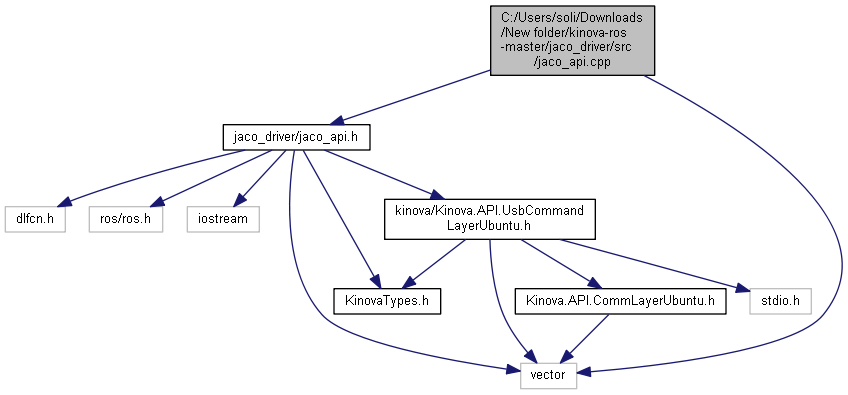
\includegraphics[width=350pt]{d1/dda/jaco__api_8cpp__incl}
\end{center}
\end{figure}
\subsection*{Namespaces}
\begin{DoxyCompactItemize}
\item 
 \hyperlink{namespacejaco}{jaco}
\end{DoxyCompactItemize}
\subsection*{Functions}
\begin{DoxyCompactItemize}
\item 
void $\ast$ \hyperlink{namespacejaco_ac891d6a7bd4014a514126248d0191413}{jaco\+::check\+Api\+Init} (void $\ast$usb\+Lib, const char $\ast$name)
\end{DoxyCompactItemize}

\hypertarget{jaco__arm_8cpp}{}\section{C\+:/\+Users/soli/\+Downloads/\+New folder/kinova-\/ros-\/master/jaco\+\_\+driver/src/jaco\+\_\+arm.cpp File Reference}
\label{jaco__arm_8cpp}\index{C\+:/\+Users/soli/\+Downloads/\+New folder/kinova-\/ros-\/master/jaco\+\_\+driver/src/jaco\+\_\+arm.\+cpp@{C\+:/\+Users/soli/\+Downloads/\+New folder/kinova-\/ros-\/master/jaco\+\_\+driver/src/jaco\+\_\+arm.\+cpp}}
{\ttfamily \#include \char`\"{}jaco\+\_\+driver/jaco\+\_\+arm.\+h\char`\"{}}\\*
{\ttfamily \#include $<$string$>$}\\*
{\ttfamily \#include $<$vector$>$}\\*
Include dependency graph for jaco\+\_\+arm.\+cpp\+:
% FIG 0
\subsection*{Namespaces}
\begin{DoxyCompactItemize}
\item 
 \hyperlink{namespacejaco}{jaco}
\end{DoxyCompactItemize}
\subsection*{Macros}
\begin{DoxyCompactItemize}
\item 
\#define \hyperlink{jaco__arm_8cpp_a598a3330b3c21701223ee0ca14316eca}{PI}~3.\+14159265359
\end{DoxyCompactItemize}


\subsection{Macro Definition Documentation}
\index{jaco\+\_\+arm.\+cpp@{jaco\+\_\+arm.\+cpp}!PI@{PI}}
\index{PI@{PI}!jaco\+\_\+arm.\+cpp@{jaco\+\_\+arm.\+cpp}}
\subsubsection[{\texorpdfstring{PI}{PI}}]{\setlength{\rightskip}{0pt plus 5cm}\#define PI~3.\+14159265359}\hypertarget{jaco__arm_8cpp_a598a3330b3c21701223ee0ca14316eca}{}\label{jaco__arm_8cpp_a598a3330b3c21701223ee0ca14316eca}

\hypertarget{jaco__arm__kinematics_8cpp}{}\section{C\+:/\+Users/soli/\+Downloads/\+New folder/kinova-\/ros-\/master/jaco\+\_\+driver/src/jaco\+\_\+arm\+\_\+kinematics.cpp File Reference}
\label{jaco__arm__kinematics_8cpp}\index{C\+:/\+Users/soli/\+Downloads/\+New folder/kinova-\/ros-\/master/jaco\+\_\+driver/src/jaco\+\_\+arm\+\_\+kinematics.\+cpp@{C\+:/\+Users/soli/\+Downloads/\+New folder/kinova-\/ros-\/master/jaco\+\_\+driver/src/jaco\+\_\+arm\+\_\+kinematics.\+cpp}}
{\ttfamily \#include $<$jaco\+\_\+driver/jaco\+\_\+arm\+\_\+kinematics.\+h$>$}\\*
{\ttfamily \#include $<$string$>$}\\*
Include dependency graph for jaco\+\_\+arm\+\_\+kinematics.\+cpp\+:
% FIG 0
\subsection*{Namespaces}
\begin{DoxyCompactItemize}
\item 
 \hyperlink{namespacejaco}{jaco}
\end{DoxyCompactItemize}
\subsection*{Functions}
\begin{DoxyCompactItemize}
\item 
std\+::string \hyperlink{namespacejaco_a6320c11725be13d2957c4e3f474d62f8}{jaco\+::concat\+Tf\+Name} (const std\+::string \&prefix, const std\+::string name)
\end{DoxyCompactItemize}

\hypertarget{jaco__comm_8cpp}{}\section{C\+:/\+Users/soli/\+Downloads/\+New folder/kinova-\/ros-\/master/jaco\+\_\+driver/src/jaco\+\_\+comm.cpp File Reference}
\label{jaco__comm_8cpp}\index{C\+:/\+Users/soli/\+Downloads/\+New folder/kinova-\/ros-\/master/jaco\+\_\+driver/src/jaco\+\_\+comm.\+cpp@{C\+:/\+Users/soli/\+Downloads/\+New folder/kinova-\/ros-\/master/jaco\+\_\+driver/src/jaco\+\_\+comm.\+cpp}}
{\ttfamily \#include $<$ros/ros.\+h$>$}\\*
{\ttfamily \#include \char`\"{}jaco\+\_\+driver/jaco\+\_\+comm.\+h\char`\"{}}\\*
{\ttfamily \#include $<$string$>$}\\*
{\ttfamily \#include $<$vector$>$}\\*
Include dependency graph for jaco\+\_\+comm.\+cpp\+:
% FIG 0
\subsection*{Namespaces}
\begin{DoxyCompactItemize}
\item 
 \hyperlink{namespacejaco}{jaco}
\end{DoxyCompactItemize}

\hypertarget{jaco__fingers__action_8cpp}{}\section{C\+:/\+Users/soli/\+Downloads/\+New folder/kinova-\/ros-\/master/jaco\+\_\+driver/src/jaco\+\_\+fingers\+\_\+action.cpp File Reference}
\label{jaco__fingers__action_8cpp}\index{C\+:/\+Users/soli/\+Downloads/\+New folder/kinova-\/ros-\/master/jaco\+\_\+driver/src/jaco\+\_\+fingers\+\_\+action.\+cpp@{C\+:/\+Users/soli/\+Downloads/\+New folder/kinova-\/ros-\/master/jaco\+\_\+driver/src/jaco\+\_\+fingers\+\_\+action.\+cpp}}
{\ttfamily \#include $<$kinova/\+Kinova\+Types.\+h$>$}\\*
{\ttfamily \#include \char`\"{}jaco\+\_\+driver/jaco\+\_\+fingers\+\_\+action.\+h\char`\"{}}\\*
{\ttfamily \#include \char`\"{}jaco\+\_\+driver/jaco\+\_\+types.\+h\char`\"{}}\\*
Include dependency graph for jaco\+\_\+fingers\+\_\+action.\+cpp\+:
% FIG 0
\subsection*{Namespaces}
\begin{DoxyCompactItemize}
\item 
 \hyperlink{namespacejaco}{jaco}
\end{DoxyCompactItemize}

\hypertarget{jaco__pose__action_8cpp}{}\section{C\+:/\+Users/soli/\+Downloads/\+New folder/kinova-\/ros-\/master/jaco\+\_\+driver/src/jaco\+\_\+pose\+\_\+action.cpp File Reference}
\label{jaco__pose__action_8cpp}\index{C\+:/\+Users/soli/\+Downloads/\+New folder/kinova-\/ros-\/master/jaco\+\_\+driver/src/jaco\+\_\+pose\+\_\+action.\+cpp@{C\+:/\+Users/soli/\+Downloads/\+New folder/kinova-\/ros-\/master/jaco\+\_\+driver/src/jaco\+\_\+pose\+\_\+action.\+cpp}}
{\ttfamily \#include \char`\"{}jaco\+\_\+driver/jaco\+\_\+pose\+\_\+action.\+h\char`\"{}}\\*
{\ttfamily \#include $<$kinova/\+Kinova\+Types.\+h$>$}\\*
{\ttfamily \#include \char`\"{}jaco\+\_\+driver/jaco\+\_\+types.\+h\char`\"{}}\\*
{\ttfamily \#include $<$string$>$}\\*
Include dependency graph for jaco\+\_\+pose\+\_\+action.\+cpp\+:
% FIG 0
\subsection*{Namespaces}
\begin{DoxyCompactItemize}
\item 
 \hyperlink{namespacejaco}{jaco}
\end{DoxyCompactItemize}

\hypertarget{jaco__types_8cpp}{}\section{D\+:/\+Longfei/\+Desktop/catkin\+\_\+\+Kinova\+R\+O\+S/src/jaco-\/ros/jaco\+\_\+driver/src/jaco\+\_\+types.cpp File Reference}
\label{jaco__types_8cpp}\index{D\+:/\+Longfei/\+Desktop/catkin\+\_\+\+Kinova\+R\+O\+S/src/jaco-\/ros/jaco\+\_\+driver/src/jaco\+\_\+types.\+cpp@{D\+:/\+Longfei/\+Desktop/catkin\+\_\+\+Kinova\+R\+O\+S/src/jaco-\/ros/jaco\+\_\+driver/src/jaco\+\_\+types.\+cpp}}
{\ttfamily \#include $<$math.\+h$>$}\\*
{\ttfamily \#include $<$angles/angles.\+h$>$}\\*
{\ttfamily \#include $<$tf/tf.\+h$>$}\\*
{\ttfamily \#include $<$jaco\+\_\+driver/jaco\+\_\+types.\+h$>$}\\*
{\ttfamily \#include $<$string$>$}\\*
Include dependency graph for jaco\+\_\+types.\+cpp\+:
\nopagebreak
\begin{figure}[H]
\begin{center}
\leavevmode
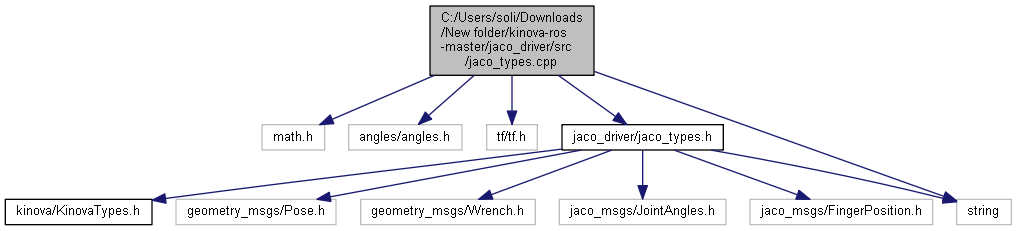
\includegraphics[width=350pt]{da/dab/jaco__types_8cpp__incl}
\end{center}
\end{figure}
\subsection*{Namespaces}
\begin{DoxyCompactItemize}
\item 
 \hyperlink{namespacejaco}{jaco}
\end{DoxyCompactItemize}
\subsection*{Functions}
\begin{DoxyCompactItemize}
\item 
bool \hyperlink{namespacejaco_a09e679eeb93252a2cf092b064e724125}{jaco\+::are\+Values\+Close} (float first, float second, float tolerance)
\item 
float \hyperlink{namespacejaco_a3e97ea63ad53f1e71821c5eee9346224}{jaco\+::normalize\+In\+Degrees} (float degrees)
\item 
float \hyperlink{namespacejaco_a564cf022c0783972c60ed14cfbc02a2a}{jaco\+::normalize\+In\+Rads} (float rads)
\item 
float \hyperlink{namespacejaco_aad452eaf0313477fc5c5b403de174118}{jaco\+::normalize\+Positive\+In\+Degrees} (float degrees)
\end{DoxyCompactItemize}

\hypertarget{jaco__arm__driver_8cpp}{}\section{C\+:/\+Users/soli/\+Downloads/\+New folder/kinova-\/ros-\/master/jaco\+\_\+driver/src/nodes/jaco\+\_\+arm\+\_\+driver.cpp File Reference}
\label{jaco__arm__driver_8cpp}\index{C\+:/\+Users/soli/\+Downloads/\+New folder/kinova-\/ros-\/master/jaco\+\_\+driver/src/nodes/jaco\+\_\+arm\+\_\+driver.\+cpp@{C\+:/\+Users/soli/\+Downloads/\+New folder/kinova-\/ros-\/master/jaco\+\_\+driver/src/nodes/jaco\+\_\+arm\+\_\+driver.\+cpp}}
{\ttfamily \#include \char`\"{}jaco\+\_\+driver/jaco\+\_\+api.\+h\char`\"{}}\\*
{\ttfamily \#include \char`\"{}jaco\+\_\+driver/jaco\+\_\+arm.\+h\char`\"{}}\\*
{\ttfamily \#include \char`\"{}jaco\+\_\+driver/jaco\+\_\+pose\+\_\+action.\+h\char`\"{}}\\*
{\ttfamily \#include \char`\"{}jaco\+\_\+driver/jaco\+\_\+angles\+\_\+action.\+h\char`\"{}}\\*
{\ttfamily \#include \char`\"{}jaco\+\_\+driver/jaco\+\_\+fingers\+\_\+action.\+h\char`\"{}}\\*
Include dependency graph for jaco\+\_\+arm\+\_\+driver.\+cpp\+:
% FIG 0
\subsection*{Functions}
\begin{DoxyCompactItemize}
\item 
int \hyperlink{jaco__arm__driver_8cpp_a3c04138a5bfe5d72780bb7e82a18e627}{main} (int argc, char $\ast$$\ast$argv)
\end{DoxyCompactItemize}


\subsection{Function Documentation}
\index{jaco\+\_\+arm\+\_\+driver.\+cpp@{jaco\+\_\+arm\+\_\+driver.\+cpp}!main@{main}}
\index{main@{main}!jaco\+\_\+arm\+\_\+driver.\+cpp@{jaco\+\_\+arm\+\_\+driver.\+cpp}}
\subsubsection[{\texorpdfstring{main(int argc, char $\ast$$\ast$argv)}{main(int argc, char **argv)}}]{\setlength{\rightskip}{0pt plus 5cm}int main (
\begin{DoxyParamCaption}
\item[{int}]{argc, }
\item[{char $\ast$$\ast$}]{argv}
\end{DoxyParamCaption}
)}\hypertarget{jaco__arm__driver_8cpp_a3c04138a5bfe5d72780bb7e82a18e627}{}\label{jaco__arm__driver_8cpp_a3c04138a5bfe5d72780bb7e82a18e627}

\hypertarget{jaco__tf__updater_8cpp}{}\section{C\+:/\+Users/soli/\+Downloads/\+New folder/kinova-\/ros-\/master/jaco\+\_\+driver/src/nodes/jaco\+\_\+tf\+\_\+updater.cpp File Reference}
\label{jaco__tf__updater_8cpp}\index{C\+:/\+Users/soli/\+Downloads/\+New folder/kinova-\/ros-\/master/jaco\+\_\+driver/src/nodes/jaco\+\_\+tf\+\_\+updater.\+cpp@{C\+:/\+Users/soli/\+Downloads/\+New folder/kinova-\/ros-\/master/jaco\+\_\+driver/src/nodes/jaco\+\_\+tf\+\_\+updater.\+cpp}}
{\ttfamily \#include $<$jaco\+\_\+driver/jaco\+\_\+tf\+\_\+updater.\+h$>$}\\*
Include dependency graph for jaco\+\_\+tf\+\_\+updater.\+cpp\+:
% FIG 0
\subsection*{Namespaces}
\begin{DoxyCompactItemize}
\item 
 \hyperlink{namespacejaco}{jaco}
\end{DoxyCompactItemize}
\subsection*{Functions}
\begin{DoxyCompactItemize}
\item 
int \hyperlink{jaco__tf__updater_8cpp_a3c04138a5bfe5d72780bb7e82a18e627}{main} (int argc, char $\ast$$\ast$argv)
\end{DoxyCompactItemize}


\subsection{Function Documentation}
\index{jaco\+\_\+tf\+\_\+updater.\+cpp@{jaco\+\_\+tf\+\_\+updater.\+cpp}!main@{main}}
\index{main@{main}!jaco\+\_\+tf\+\_\+updater.\+cpp@{jaco\+\_\+tf\+\_\+updater.\+cpp}}
\subsubsection[{\texorpdfstring{main(int argc, char $\ast$$\ast$argv)}{main(int argc, char **argv)}}]{\setlength{\rightskip}{0pt plus 5cm}int main (
\begin{DoxyParamCaption}
\item[{int}]{argc, }
\item[{char $\ast$$\ast$}]{argv}
\end{DoxyParamCaption}
)}\hypertarget{jaco__tf__updater_8cpp_a3c04138a5bfe5d72780bb7e82a18e627}{}\label{jaco__tf__updater_8cpp_a3c04138a5bfe5d72780bb7e82a18e627}

\hypertarget{test__jaco__arm__car__vel_8cpp}{}\section{C\+:/\+Users/soli/\+Downloads/\+New folder/kinova-\/ros-\/master/jaco\+\_\+driver/src/testers/test\+\_\+jaco\+\_\+arm\+\_\+car\+\_\+vel.cpp File Reference}
\label{test__jaco__arm__car__vel_8cpp}\index{C\+:/\+Users/soli/\+Downloads/\+New folder/kinova-\/ros-\/master/jaco\+\_\+driver/src/testers/test\+\_\+jaco\+\_\+arm\+\_\+car\+\_\+vel.\+cpp@{C\+:/\+Users/soli/\+Downloads/\+New folder/kinova-\/ros-\/master/jaco\+\_\+driver/src/testers/test\+\_\+jaco\+\_\+arm\+\_\+car\+\_\+vel.\+cpp}}
{\ttfamily \#include $<$jaco\+\_\+driver/test\+\_\+jaco\+\_\+arm\+\_\+car\+\_\+vel.\+h$>$}\\*
Include dependency graph for test\+\_\+jaco\+\_\+arm\+\_\+car\+\_\+vel.\+cpp\+:
% FIG 0
\subsection*{Functions}
\begin{DoxyCompactItemize}
\item 
int \hyperlink{test__jaco__arm__car__vel_8cpp_a3c04138a5bfe5d72780bb7e82a18e627}{main} (int argc, char $\ast$$\ast$argv)
\end{DoxyCompactItemize}


\subsection{Function Documentation}
\index{test\+\_\+jaco\+\_\+arm\+\_\+car\+\_\+vel.\+cpp@{test\+\_\+jaco\+\_\+arm\+\_\+car\+\_\+vel.\+cpp}!main@{main}}
\index{main@{main}!test\+\_\+jaco\+\_\+arm\+\_\+car\+\_\+vel.\+cpp@{test\+\_\+jaco\+\_\+arm\+\_\+car\+\_\+vel.\+cpp}}
\subsubsection[{\texorpdfstring{main(int argc, char $\ast$$\ast$argv)}{main(int argc, char **argv)}}]{\setlength{\rightskip}{0pt plus 5cm}int main (
\begin{DoxyParamCaption}
\item[{int}]{argc, }
\item[{char $\ast$$\ast$}]{argv}
\end{DoxyParamCaption}
)}\hypertarget{test__jaco__arm__car__vel_8cpp_a3c04138a5bfe5d72780bb7e82a18e627}{}\label{test__jaco__arm__car__vel_8cpp_a3c04138a5bfe5d72780bb7e82a18e627}
String containing the topic name for cartesian commands 
\hypertarget{test__jaco__arm__controller_8cpp}{}\section{D\+:/\+Longfei/\+Desktop/catkin\+\_\+\+Kinova\+R\+O\+S/src/jaco-\/ros/jaco\+\_\+driver/src/testers/test\+\_\+jaco\+\_\+arm\+\_\+controller.cpp File Reference}
\label{test__jaco__arm__controller_8cpp}\index{D\+:/\+Longfei/\+Desktop/catkin\+\_\+\+Kinova\+R\+O\+S/src/jaco-\/ros/jaco\+\_\+driver/src/testers/test\+\_\+jaco\+\_\+arm\+\_\+controller.\+cpp@{D\+:/\+Longfei/\+Desktop/catkin\+\_\+\+Kinova\+R\+O\+S/src/jaco-\/ros/jaco\+\_\+driver/src/testers/test\+\_\+jaco\+\_\+arm\+\_\+controller.\+cpp}}
{\ttfamily \#include $<$geometry\+\_\+msgs/\+Pose\+Stamped.\+h$>$}\\*
{\ttfamily \#include $<$geometry\+\_\+msgs/\+Twist\+Stamped.\+h$>$}\\*
{\ttfamily \#include $<$tf/tf.\+h$>$}\\*
{\ttfamily \#include $<$ros/ros.\+h$>$}\\*
{\ttfamily \#include $<$jaco\+\_\+driver/\+Jaco\+Position\+Config.\+h$>$}\\*
{\ttfamily \#include $<$dynamic\+\_\+reconfigure/server.\+h$>$}\\*
Include dependency graph for test\+\_\+jaco\+\_\+arm\+\_\+controller.\+cpp\+:
\nopagebreak
\begin{figure}[H]
\begin{center}
\leavevmode
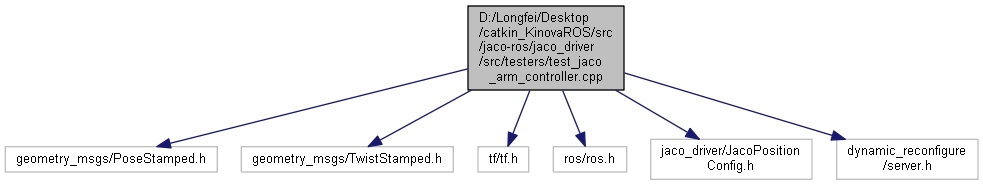
\includegraphics[width=350pt]{d1/d3e/test__jaco__arm__controller_8cpp__incl}
\end{center}
\end{figure}
\subsection*{Functions}
\begin{DoxyCompactItemize}
\item 
void \hyperlink{test__jaco__arm__controller_8cpp_a9b22877867bb7fee9e5a33831d4f5151}{callback} (jaco\+\_\+driver\+::\+Jaco\+Position\+Config \&config, uint32\+\_\+t level)
\item 
int \hyperlink{test__jaco__arm__controller_8cpp_a3c04138a5bfe5d72780bb7e82a18e627}{main} (int argc, char $\ast$$\ast$argv)
\item 
void \hyperlink{test__jaco__arm__controller_8cpp_a555d06d88fe912826cb143b1eb9b595f}{Timer\+Callback} (const ros\+::\+Timer\+Event \&)
\end{DoxyCompactItemize}
\subsection*{Variables}
\begin{DoxyCompactItemize}
\item 
ros\+::\+Publisher $\ast$ \hyperlink{test__jaco__arm__controller_8cpp_ad5e5d8e14bfcad1c0cc878616783a7e2}{pub}
\item 
float \hyperlink{test__jaco__arm__controller_8cpp_a7018d450f1b8ac16e05c9f60ff2c5e5c}{rx\+\_\+pose} =0
\item 
float \hyperlink{test__jaco__arm__controller_8cpp_abf857bc7e68483191c2e2c3e91ac5f4c}{ry\+\_\+pose} =0
\item 
float \hyperlink{test__jaco__arm__controller_8cpp_aba5846c38922e0154087cc48943e9e97}{rz\+\_\+pose} =0
\item 
float \hyperlink{test__jaco__arm__controller_8cpp_a1b673edb7bae9a685deb9beeaf306434}{x\+\_\+pose} =0
\item 
float \hyperlink{test__jaco__arm__controller_8cpp_a691b31f8e26c353862266520fbb806e7}{y\+\_\+pose} =0
\item 
float \hyperlink{test__jaco__arm__controller_8cpp_a1d00778dfc07f0b53fdcdc73754e7ffc}{z\+\_\+pose} =0
\end{DoxyCompactItemize}


\subsection{Function Documentation}
\index{test\+\_\+jaco\+\_\+arm\+\_\+controller.\+cpp@{test\+\_\+jaco\+\_\+arm\+\_\+controller.\+cpp}!callback@{callback}}
\index{callback@{callback}!test\+\_\+jaco\+\_\+arm\+\_\+controller.\+cpp@{test\+\_\+jaco\+\_\+arm\+\_\+controller.\+cpp}}
\subsubsection[{\texorpdfstring{callback(jaco\+\_\+driver\+::\+Jaco\+Position\+Config \&config, uint32\+\_\+t level)}{callback(jaco_driver::JacoPositionConfig &config, uint32_t level)}}]{\setlength{\rightskip}{0pt plus 5cm}void callback (
\begin{DoxyParamCaption}
\item[{jaco\+\_\+driver\+::\+Jaco\+Position\+Config \&}]{config, }
\item[{uint32\+\_\+t}]{level}
\end{DoxyParamCaption}
)}\hypertarget{test__jaco__arm__controller_8cpp_a9b22877867bb7fee9e5a33831d4f5151}{}\label{test__jaco__arm__controller_8cpp_a9b22877867bb7fee9e5a33831d4f5151}

\begin{DoxyCode}
38                                                                      \{
39 
40      \hyperlink{test__jaco__arm__controller_8cpp_a1b673edb7bae9a685deb9beeaf306434}{x\_pose}=config.X\_Pose;
41      \hyperlink{test__jaco__arm__controller_8cpp_a691b31f8e26c353862266520fbb806e7}{y\_pose}=config.Y\_Pose;
42      \hyperlink{test__jaco__arm__controller_8cpp_a1d00778dfc07f0b53fdcdc73754e7ffc}{z\_pose}=config.Z\_Pose;
43      \hyperlink{test__jaco__arm__controller_8cpp_a7018d450f1b8ac16e05c9f60ff2c5e5c}{rx\_pose}=config.RX\_Pose;
44      \hyperlink{test__jaco__arm__controller_8cpp_abf857bc7e68483191c2e2c3e91ac5f4c}{ry\_pose}=config.RY\_Pose;
45      \hyperlink{test__jaco__arm__controller_8cpp_aba5846c38922e0154087cc48943e9e97}{rz\_pose}=config.RZ\_Pose;
46 
47     \textcolor{comment}{//  ROS\_INFO("Reconfigure");}
48 
49 
50 \}
\end{DoxyCode}
\index{test\+\_\+jaco\+\_\+arm\+\_\+controller.\+cpp@{test\+\_\+jaco\+\_\+arm\+\_\+controller.\+cpp}!main@{main}}
\index{main@{main}!test\+\_\+jaco\+\_\+arm\+\_\+controller.\+cpp@{test\+\_\+jaco\+\_\+arm\+\_\+controller.\+cpp}}
\subsubsection[{\texorpdfstring{main(int argc, char $\ast$$\ast$argv)}{main(int argc, char **argv)}}]{\setlength{\rightskip}{0pt plus 5cm}int main (
\begin{DoxyParamCaption}
\item[{int}]{argc, }
\item[{char $\ast$$\ast$}]{argv}
\end{DoxyParamCaption}
)}\hypertarget{test__jaco__arm__controller_8cpp_a3c04138a5bfe5d72780bb7e82a18e627}{}\label{test__jaco__arm__controller_8cpp_a3c04138a5bfe5d72780bb7e82a18e627}
String containing the topic name for cartesian commands 
\begin{DoxyCode}
73                                 \{
74 
75     \textcolor{comment}{/* Set up ROS */}
76     ros::init(argc, argv, \textcolor{stringliteral}{"test\_jaco\_arm\_controller"});
77     ros::NodeHandle nh;
78     ros::NodeHandle param\_nh(\textcolor{stringliteral}{"~"});
79 
80     std::string ArmPose(\textcolor{stringliteral}{"object\_pose"}); 
81 
82     ros::Publisher pub2 = nh.advertise<geometry\_msgs::PoseStamped>(ArmPose,
83             2);
84 
85     \hyperlink{test__jaco__arm__controller_8cpp_ad5e5d8e14bfcad1c0cc878616783a7e2}{pub} = &pub2;
86     dynamic\_reconfigure::Server<jaco\_driver::JacoPositionConfig>  dr\_server;
87  dynamic\_reconfigure::Server<jaco\_driver::JacoPositionConfig>::CallbackType dr\_call = boost::bind(&
      \hyperlink{test__jaco__arm__controller_8cpp_a9b22877867bb7fee9e5a33831d4f5151}{callback}, \_1, \_2);
88     dr\_server.setCallback(dr\_call);
89       ros::Timer    timer = nh.createTimer(ros::Duration(0.1),&\hyperlink{test__jaco__arm__controller_8cpp_a555d06d88fe912826cb143b1eb9b595f}{TimerCallback});
90 
91         ros::spin();
92 
93 \}
\end{DoxyCode}
\index{test\+\_\+jaco\+\_\+arm\+\_\+controller.\+cpp@{test\+\_\+jaco\+\_\+arm\+\_\+controller.\+cpp}!Timer\+Callback@{Timer\+Callback}}
\index{Timer\+Callback@{Timer\+Callback}!test\+\_\+jaco\+\_\+arm\+\_\+controller.\+cpp@{test\+\_\+jaco\+\_\+arm\+\_\+controller.\+cpp}}
\subsubsection[{\texorpdfstring{Timer\+Callback(const ros\+::\+Timer\+Event \&)}{TimerCallback(const ros::TimerEvent &)}}]{\setlength{\rightskip}{0pt plus 5cm}void Cartesian\+Vel\+Test\+::\+Timer\+Callback (
\begin{DoxyParamCaption}
\item[{const ros\+::\+Timer\+Event \&}]{}
\end{DoxyParamCaption}
)}\hypertarget{test__jaco__arm__controller_8cpp_a555d06d88fe912826cb143b1eb9b595f}{}\label{test__jaco__arm__controller_8cpp_a555d06d88fe912826cb143b1eb9b595f}

\begin{DoxyCode}
55 \{
56     geometry\_msgs::PoseStamped test\_msg;
57 
58             test\_msg.pose.position.x = \hyperlink{test__jaco__arm__controller_8cpp_a1b673edb7bae9a685deb9beeaf306434}{x\_pose};
59             test\_msg.pose.position.y = \hyperlink{test__jaco__arm__controller_8cpp_a691b31f8e26c353862266520fbb806e7}{y\_pose};
60             test\_msg.pose.position.z = \hyperlink{test__jaco__arm__controller_8cpp_a1d00778dfc07f0b53fdcdc73754e7ffc}{z\_pose};
61 
62             tf::Quaternion q;
63 
64             q.setRPY(\hyperlink{test__jaco__arm__controller_8cpp_a7018d450f1b8ac16e05c9f60ff2c5e5c}{rx\_pose},\hyperlink{test__jaco__arm__controller_8cpp_abf857bc7e68483191c2e2c3e91ac5f4c}{ry\_pose},\hyperlink{test__jaco__arm__controller_8cpp_aba5846c38922e0154087cc48943e9e97}{rz\_pose});
65 
66             tf::quaternionTFToMsg(q,test\_msg.pose.orientation);
67             test\_msg.header.frame\_id = \textcolor{stringliteral}{"/arm\_base"};
68             test\_msg.header.stamp = ros::Time().now();
69             \hyperlink{test__jaco__arm__controller_8cpp_ad5e5d8e14bfcad1c0cc878616783a7e2}{pub}->publish(test\_msg);
70 
71 \}
\end{DoxyCode}


\subsection{Variable Documentation}
\index{test\+\_\+jaco\+\_\+arm\+\_\+controller.\+cpp@{test\+\_\+jaco\+\_\+arm\+\_\+controller.\+cpp}!pub@{pub}}
\index{pub@{pub}!test\+\_\+jaco\+\_\+arm\+\_\+controller.\+cpp@{test\+\_\+jaco\+\_\+arm\+\_\+controller.\+cpp}}
\subsubsection[{\texorpdfstring{pub}{pub}}]{\setlength{\rightskip}{0pt plus 5cm}ros\+::\+Publisher$\ast$ pub}\hypertarget{test__jaco__arm__controller_8cpp_ad5e5d8e14bfcad1c0cc878616783a7e2}{}\label{test__jaco__arm__controller_8cpp_ad5e5d8e14bfcad1c0cc878616783a7e2}
\index{test\+\_\+jaco\+\_\+arm\+\_\+controller.\+cpp@{test\+\_\+jaco\+\_\+arm\+\_\+controller.\+cpp}!rx\+\_\+pose@{rx\+\_\+pose}}
\index{rx\+\_\+pose@{rx\+\_\+pose}!test\+\_\+jaco\+\_\+arm\+\_\+controller.\+cpp@{test\+\_\+jaco\+\_\+arm\+\_\+controller.\+cpp}}
\subsubsection[{\texorpdfstring{rx\+\_\+pose}{rx_pose}}]{\setlength{\rightskip}{0pt plus 5cm}float rx\+\_\+pose =0}\hypertarget{test__jaco__arm__controller_8cpp_a7018d450f1b8ac16e05c9f60ff2c5e5c}{}\label{test__jaco__arm__controller_8cpp_a7018d450f1b8ac16e05c9f60ff2c5e5c}
\index{test\+\_\+jaco\+\_\+arm\+\_\+controller.\+cpp@{test\+\_\+jaco\+\_\+arm\+\_\+controller.\+cpp}!ry\+\_\+pose@{ry\+\_\+pose}}
\index{ry\+\_\+pose@{ry\+\_\+pose}!test\+\_\+jaco\+\_\+arm\+\_\+controller.\+cpp@{test\+\_\+jaco\+\_\+arm\+\_\+controller.\+cpp}}
\subsubsection[{\texorpdfstring{ry\+\_\+pose}{ry_pose}}]{\setlength{\rightskip}{0pt plus 5cm}float ry\+\_\+pose =0}\hypertarget{test__jaco__arm__controller_8cpp_abf857bc7e68483191c2e2c3e91ac5f4c}{}\label{test__jaco__arm__controller_8cpp_abf857bc7e68483191c2e2c3e91ac5f4c}
\index{test\+\_\+jaco\+\_\+arm\+\_\+controller.\+cpp@{test\+\_\+jaco\+\_\+arm\+\_\+controller.\+cpp}!rz\+\_\+pose@{rz\+\_\+pose}}
\index{rz\+\_\+pose@{rz\+\_\+pose}!test\+\_\+jaco\+\_\+arm\+\_\+controller.\+cpp@{test\+\_\+jaco\+\_\+arm\+\_\+controller.\+cpp}}
\subsubsection[{\texorpdfstring{rz\+\_\+pose}{rz_pose}}]{\setlength{\rightskip}{0pt plus 5cm}float rz\+\_\+pose =0}\hypertarget{test__jaco__arm__controller_8cpp_aba5846c38922e0154087cc48943e9e97}{}\label{test__jaco__arm__controller_8cpp_aba5846c38922e0154087cc48943e9e97}
\index{test\+\_\+jaco\+\_\+arm\+\_\+controller.\+cpp@{test\+\_\+jaco\+\_\+arm\+\_\+controller.\+cpp}!x\+\_\+pose@{x\+\_\+pose}}
\index{x\+\_\+pose@{x\+\_\+pose}!test\+\_\+jaco\+\_\+arm\+\_\+controller.\+cpp@{test\+\_\+jaco\+\_\+arm\+\_\+controller.\+cpp}}
\subsubsection[{\texorpdfstring{x\+\_\+pose}{x_pose}}]{\setlength{\rightskip}{0pt plus 5cm}float x\+\_\+pose =0}\hypertarget{test__jaco__arm__controller_8cpp_a1b673edb7bae9a685deb9beeaf306434}{}\label{test__jaco__arm__controller_8cpp_a1b673edb7bae9a685deb9beeaf306434}
\index{test\+\_\+jaco\+\_\+arm\+\_\+controller.\+cpp@{test\+\_\+jaco\+\_\+arm\+\_\+controller.\+cpp}!y\+\_\+pose@{y\+\_\+pose}}
\index{y\+\_\+pose@{y\+\_\+pose}!test\+\_\+jaco\+\_\+arm\+\_\+controller.\+cpp@{test\+\_\+jaco\+\_\+arm\+\_\+controller.\+cpp}}
\subsubsection[{\texorpdfstring{y\+\_\+pose}{y_pose}}]{\setlength{\rightskip}{0pt plus 5cm}float y\+\_\+pose =0}\hypertarget{test__jaco__arm__controller_8cpp_a691b31f8e26c353862266520fbb806e7}{}\label{test__jaco__arm__controller_8cpp_a691b31f8e26c353862266520fbb806e7}
\index{test\+\_\+jaco\+\_\+arm\+\_\+controller.\+cpp@{test\+\_\+jaco\+\_\+arm\+\_\+controller.\+cpp}!z\+\_\+pose@{z\+\_\+pose}}
\index{z\+\_\+pose@{z\+\_\+pose}!test\+\_\+jaco\+\_\+arm\+\_\+controller.\+cpp@{test\+\_\+jaco\+\_\+arm\+\_\+controller.\+cpp}}
\subsubsection[{\texorpdfstring{z\+\_\+pose}{z_pose}}]{\setlength{\rightskip}{0pt plus 5cm}float z\+\_\+pose =0}\hypertarget{test__jaco__arm__controller_8cpp_a1d00778dfc07f0b53fdcdc73754e7ffc}{}\label{test__jaco__arm__controller_8cpp_a1d00778dfc07f0b53fdcdc73754e7ffc}

\hypertarget{test__jaco__arm__vel_8cpp}{}\section{D\+:/\+Longfei/\+Desktop/catkin\+\_\+\+Kinova\+R\+O\+S/src/jaco-\/ros/jaco\+\_\+driver/src/testers/test\+\_\+jaco\+\_\+arm\+\_\+vel.cpp File Reference}
\label{test__jaco__arm__vel_8cpp}\index{D\+:/\+Longfei/\+Desktop/catkin\+\_\+\+Kinova\+R\+O\+S/src/jaco-\/ros/jaco\+\_\+driver/src/testers/test\+\_\+jaco\+\_\+arm\+\_\+vel.\+cpp@{D\+:/\+Longfei/\+Desktop/catkin\+\_\+\+Kinova\+R\+O\+S/src/jaco-\/ros/jaco\+\_\+driver/src/testers/test\+\_\+jaco\+\_\+arm\+\_\+vel.\+cpp}}
{\ttfamily \#include $<$geometry\+\_\+msgs/\+Pose\+Stamped.\+h$>$}\\*
{\ttfamily \#include $<$geometry\+\_\+msgs/\+Twist\+Stamped.\+h$>$}\\*
{\ttfamily \#include $<$tf/tf.\+h$>$}\\*
{\ttfamily \#include $<$ros/ros.\+h$>$}\\*
{\ttfamily \#include $<$jaco\+\_\+msgs/cartesian\+\_\+velocity.\+h$>$}\\*
Include dependency graph for test\+\_\+jaco\+\_\+arm\+\_\+vel.\+cpp\+:
\nopagebreak
\begin{figure}[H]
\begin{center}
\leavevmode
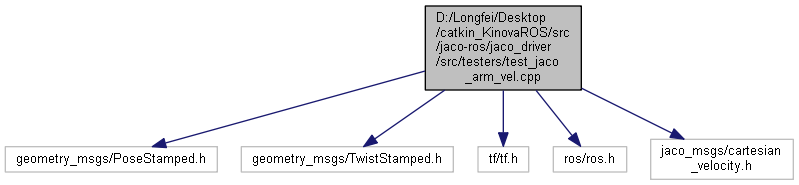
\includegraphics[width=350pt]{db/dda/test__jaco__arm__vel_8cpp__incl}
\end{center}
\end{figure}
\subsection*{Functions}
\begin{DoxyCompactItemize}
\item 
int \hyperlink{test__jaco__arm__vel_8cpp_a3c04138a5bfe5d72780bb7e82a18e627}{main} (int argc, char $\ast$$\ast$argv)
\item 
void \hyperlink{test__jaco__arm__vel_8cpp_acaaff023b0d196868429ae4d95cced23}{Timer\+Callback} (const ros\+::\+Timer\+Event \&)
\end{DoxyCompactItemize}
\subsection*{Variables}
\begin{DoxyCompactItemize}
\item 
ros\+::\+Publisher \hyperlink{test__jaco__arm__vel_8cpp_a350594df3e8f6948c8462edfd41ce086}{pub}
\end{DoxyCompactItemize}


\subsection{Function Documentation}
\index{test\+\_\+jaco\+\_\+arm\+\_\+vel.\+cpp@{test\+\_\+jaco\+\_\+arm\+\_\+vel.\+cpp}!main@{main}}
\index{main@{main}!test\+\_\+jaco\+\_\+arm\+\_\+vel.\+cpp@{test\+\_\+jaco\+\_\+arm\+\_\+vel.\+cpp}}
\subsubsection[{\texorpdfstring{main(int argc, char $\ast$$\ast$argv)}{main(int argc, char **argv)}}]{\setlength{\rightskip}{0pt plus 5cm}int main (
\begin{DoxyParamCaption}
\item[{int}]{argc, }
\item[{char $\ast$$\ast$}]{argv}
\end{DoxyParamCaption}
)}\hypertarget{test__jaco__arm__vel_8cpp_a3c04138a5bfe5d72780bb7e82a18e627}{}\label{test__jaco__arm__vel_8cpp_a3c04138a5bfe5d72780bb7e82a18e627}
String containing the topic name for cartesian commands 
\begin{DoxyCode}
43                                 \{
44 
45     \textcolor{comment}{/* Set up ROS */}
46     ros::init(argc, argv, \textcolor{stringliteral}{"test\_jaco\_arm\_vel"});
47     ros::NodeHandle nh;
48     ros::NodeHandle param\_nh(\textcolor{stringliteral}{"~"});
49 
50     std::string \hyperlink{namespacejaco__msgs_a3885bcb43e15bd44e269141fd88ae604}{JointVelocity}(\textcolor{stringliteral}{"CartesianVelocity"}); 
51 
52      \hyperlink{test__jaco__arm__vel_8cpp_a350594df3e8f6948c8462edfd41ce086}{pub} = nh.advertise<jaco\_msgs::cartesian\_velocity>(\hyperlink{namespacejaco__msgs_a3885bcb43e15bd44e269141fd88ae604}{JointVelocity},
53             2);
54 
55     ros::Timer timer = nh.createTimer(ros::Duration(0.01),\hyperlink{test__jaco__arm__vel_8cpp_acaaff023b0d196868429ae4d95cced23}{TimerCallback});
56 
57 
58     ros::spin();
59 \}
\end{DoxyCode}
\index{test\+\_\+jaco\+\_\+arm\+\_\+vel.\+cpp@{test\+\_\+jaco\+\_\+arm\+\_\+vel.\+cpp}!Timer\+Callback@{Timer\+Callback}}
\index{Timer\+Callback@{Timer\+Callback}!test\+\_\+jaco\+\_\+arm\+\_\+vel.\+cpp@{test\+\_\+jaco\+\_\+arm\+\_\+vel.\+cpp}}
\subsubsection[{\texorpdfstring{Timer\+Callback(const ros\+::\+Timer\+Event \&)}{TimerCallback(const ros::TimerEvent &)}}]{\setlength{\rightskip}{0pt plus 5cm}void Timer\+Callback (
\begin{DoxyParamCaption}
\item[{const ros\+::\+Timer\+Event \&}]{}
\end{DoxyParamCaption}
)}\hypertarget{test__jaco__arm__vel_8cpp_acaaff023b0d196868429ae4d95cced23}{}\label{test__jaco__arm__vel_8cpp_acaaff023b0d196868429ae4d95cced23}

\begin{DoxyCode}
27 \{
28     jaco\_msgs::cartesian\_velocity test\_msg;
29 
30             test\_msg.Velocity\_X = 0.0;
31             test\_msg.Velocity\_Y = 10;
32             test\_msg.Velocity\_Z = 0;
33             test\_msg.Velocity\_TX = 0;
34             test\_msg.Velocity\_TY = 0;
35             test\_msg.Velocity\_TZ = 0;
36 
37 
38             \hyperlink{test__jaco__arm__vel_8cpp_a350594df3e8f6948c8462edfd41ce086}{pub}.publish(test\_msg);
39 
40 
41 \}
\end{DoxyCode}


\subsection{Variable Documentation}
\index{test\+\_\+jaco\+\_\+arm\+\_\+vel.\+cpp@{test\+\_\+jaco\+\_\+arm\+\_\+vel.\+cpp}!pub@{pub}}
\index{pub@{pub}!test\+\_\+jaco\+\_\+arm\+\_\+vel.\+cpp@{test\+\_\+jaco\+\_\+arm\+\_\+vel.\+cpp}}
\subsubsection[{\texorpdfstring{pub}{pub}}]{\setlength{\rightskip}{0pt plus 5cm}ros\+::\+Publisher pub}\hypertarget{test__jaco__arm__vel_8cpp_a350594df3e8f6948c8462edfd41ce086}{}\label{test__jaco__arm__vel_8cpp_a350594df3e8f6948c8462edfd41ce086}

\hypertarget{angle__action__client_8py}{}\section{C\+:/\+Users/soli/\+Downloads/\+New folder/kinova-\/ros-\/master/jaco\+\_\+driver/test/angle\+\_\+action\+\_\+client.py File Reference}
\label{angle__action__client_8py}\index{C\+:/\+Users/soli/\+Downloads/\+New folder/kinova-\/ros-\/master/jaco\+\_\+driver/test/angle\+\_\+action\+\_\+client.\+py@{C\+:/\+Users/soli/\+Downloads/\+New folder/kinova-\/ros-\/master/jaco\+\_\+driver/test/angle\+\_\+action\+\_\+client.\+py}}
\subsection*{Namespaces}
\begin{DoxyCompactItemize}
\item 
 \hyperlink{namespaceangle__action__client}{angle\+\_\+action\+\_\+client}
\end{DoxyCompactItemize}
\subsection*{Functions}
\begin{DoxyCompactItemize}
\item 
def \hyperlink{namespaceangle__action__client_a536654e415d43c20ff7be40b5b60f4e5}{angle\+\_\+action\+\_\+client.\+pose\+\_\+client} ()
\end{DoxyCompactItemize}
\subsection*{Variables}
\begin{DoxyCompactItemize}
\item 
\hyperlink{namespaceangle__action__client_ae4489551abd88fa0cd5250b9db7fd50e}{angle\+\_\+action\+\_\+client.\+result} = pose\+\_\+client()
\end{DoxyCompactItemize}

\hypertarget{finger__action__client_8py}{}\section{C\+:/\+Users/soli/\+Downloads/\+New folder/kinova-\/ros-\/master/jaco\+\_\+driver/test/finger\+\_\+action\+\_\+client.py File Reference}
\label{finger__action__client_8py}\index{C\+:/\+Users/soli/\+Downloads/\+New folder/kinova-\/ros-\/master/jaco\+\_\+driver/test/finger\+\_\+action\+\_\+client.\+py@{C\+:/\+Users/soli/\+Downloads/\+New folder/kinova-\/ros-\/master/jaco\+\_\+driver/test/finger\+\_\+action\+\_\+client.\+py}}
\subsection*{Namespaces}
\begin{DoxyCompactItemize}
\item 
 \hyperlink{namespacefinger__action__client}{finger\+\_\+action\+\_\+client}
\end{DoxyCompactItemize}
\subsection*{Functions}
\begin{DoxyCompactItemize}
\item 
def \hyperlink{namespacefinger__action__client_a052b0ba6f2141589b77dad69727b3246}{finger\+\_\+action\+\_\+client.\+pose\+\_\+client} ()
\end{DoxyCompactItemize}
\subsection*{Variables}
\begin{DoxyCompactItemize}
\item 
\hyperlink{namespacefinger__action__client_a457ef4f2bf118e0ad46b05a4956a496d}{finger\+\_\+action\+\_\+client.\+result} = pose\+\_\+client()
\end{DoxyCompactItemize}

\hypertarget{pose__action__client_8py}{}\section{D\+:/\+Longfei/\+Desktop/catkin\+\_\+\+Kinova\+R\+O\+S/src/jaco-\/ros/jaco\+\_\+driver/test/pose\+\_\+action\+\_\+client.py File Reference}
\label{pose__action__client_8py}\index{D\+:/\+Longfei/\+Desktop/catkin\+\_\+\+Kinova\+R\+O\+S/src/jaco-\/ros/jaco\+\_\+driver/test/pose\+\_\+action\+\_\+client.\+py@{D\+:/\+Longfei/\+Desktop/catkin\+\_\+\+Kinova\+R\+O\+S/src/jaco-\/ros/jaco\+\_\+driver/test/pose\+\_\+action\+\_\+client.\+py}}
\subsection*{Namespaces}
\begin{DoxyCompactItemize}
\item 
 \hyperlink{namespacepose__action__client}{pose\+\_\+action\+\_\+client}
\end{DoxyCompactItemize}
\subsection*{Functions}
\begin{DoxyCompactItemize}
\item 
def \hyperlink{namespacepose__action__client_a2379b6420c9b26d36eff80d2c269ce09}{pose\+\_\+action\+\_\+client.\+pose\+\_\+client} ()
\end{DoxyCompactItemize}
\subsection*{Variables}
\begin{DoxyCompactItemize}
\item 
\hyperlink{namespacepose__action__client_af6e1b48c2733e83789035d19de147d40}{pose\+\_\+action\+\_\+client.\+result} = pose\+\_\+client()
\end{DoxyCompactItemize}

\hypertarget{_r_e_a_d_m_e_8md}{}\section{C\+:/\+Users/soli/\+Downloads/\+New folder/kinova-\/ros-\/master/\+R\+E\+A\+D\+ME.md File Reference}
\label{_r_e_a_d_m_e_8md}\index{C\+:/\+Users/soli/\+Downloads/\+New folder/kinova-\/ros-\/master/\+R\+E\+A\+D\+M\+E.\+md@{C\+:/\+Users/soli/\+Downloads/\+New folder/kinova-\/ros-\/master/\+R\+E\+A\+D\+M\+E.\+md}}

%--- End generated contents ---

% Index
\backmatter
\newpage
\phantomsection
\clearemptydoublepage
\addcontentsline{toc}{chapter}{Index}
\printindex

\end{document}
